% Options for packages loaded elsewhere
\PassOptionsToPackage{unicode}{hyperref}
\PassOptionsToPackage{hyphens}{url}
\documentclass[
  11pt,
  a4paper,
]{article}
\usepackage{xcolor}
\usepackage[margin=22mm]{geometry}
\usepackage{amsmath,amssymb}
\setcounter{secnumdepth}{-\maxdimen} % remove section numbering
\usepackage{iftex}
\ifPDFTeX
  \usepackage[T1]{fontenc}
  \usepackage[utf8]{inputenc}
  \usepackage{textcomp} % provide euro and other symbols
\else % if luatex or xetex
  \usepackage{unicode-math} % this also loads fontspec
  \defaultfontfeatures{Scale=MatchLowercase}
  \defaultfontfeatures[\rmfamily]{Ligatures=TeX,Scale=1}
\fi
\usepackage{lmodern}
\ifPDFTeX\else
  % xetex/luatex font selection
\fi
% Use upquote if available, for straight quotes in verbatim environments
\IfFileExists{upquote.sty}{\usepackage{upquote}}{}
\IfFileExists{microtype.sty}{% use microtype if available
  \usepackage[]{microtype}
  \UseMicrotypeSet[protrusion]{basicmath} % disable protrusion for tt fonts
}{}
\makeatletter
\@ifundefined{KOMAClassName}{% if non-KOMA class
  \IfFileExists{parskip.sty}{%
    \usepackage{parskip}
  }{% else
    \setlength{\parindent}{0pt}
    \setlength{\parskip}{6pt plus 2pt minus 1pt}}
}{% if KOMA class
  \KOMAoptions{parskip=half}}
\makeatother
\usepackage{longtable,booktabs,array}
\newcounter{none} % for unnumbered tables
\usepackage{calc} % for calculating minipage widths
% Correct order of tables after \paragraph or \subparagraph
\usepackage{etoolbox}
\makeatletter
\patchcmd\longtable{\par}{\if@noskipsec\mbox{}\fi\par}{}{}
\makeatother
% Allow footnotes in longtable head/foot
\IfFileExists{footnotehyper.sty}{\usepackage{footnotehyper}}{\usepackage{footnote}}
\makesavenoteenv{longtable}
\usepackage{graphicx}
\makeatletter
\newsavebox\pandoc@box
\newcommand*\pandocbounded[1]{% scales image to fit in text height/width
  \sbox\pandoc@box{#1}%
  \Gscale@div\@tempa{\textheight}{\dimexpr\ht\pandoc@box+\dp\pandoc@box\relax}%
  \Gscale@div\@tempb{\linewidth}{\wd\pandoc@box}%
  \ifdim\@tempb\p@<\@tempa\p@\let\@tempa\@tempb\fi% select the smaller of both
  \ifdim\@tempa\p@<\p@\scalebox{\@tempa}{\usebox\pandoc@box}%
  \else\usebox{\pandoc@box}%
  \fi%
}
% Set default figure placement to htbp
\def\fps@figure{htbp}
\makeatother
\setlength{\emergencystretch}{3em} % prevent overfull lines
\providecommand{\tightlist}{%
  \setlength{\itemsep}{0pt}\setlength{\parskip}{0pt}}
\usepackage{bookmark}
\IfFileExists{xurl.sty}{\usepackage{xurl}}{} % add URL line breaks if available
\urlstyle{same}
\hypersetup{
  pdftitle={Beyond: elliptic logarithms{,} the analytic subgroup theorem{,} and open problems},
  pdfauthor={GPT-6 Astra (OpenAI), Ultra},
  hidelinks,
  pdfcreator={LaTeX via pandoc}}

\title{Beyond: elliptic logarithms, the analytic subgroup theorem, and
open problems}
\author{GPT-6 Astra (OpenAI), Ultra}
\date{October 2026}

\usepackage{mathrsfs}
\providecommand{\Eta}{\mathrm{H}}
\begin{document}
\maketitle

\emph{Mathematical exposition by GPT-6 Astra (OpenAI), Ultra. Public
domain (CC0).}

\subsection{1. Algebraic logarithms and their
relations}\label{algebraic-logarithms-and-their-relations}

The exponential map of a commutative algebraic group connects a linear
space of logarithms with an algebraic space of points. The analytic
subgroup theorem describes how an algebraic linear constraint on such a
logarithm forces an algebraic subgroup. For an additive group times a
torus, this yields Baker's theorem. For abelian varieties and their
vector extensions, it controls logarithms and periods of algebraic
differential forms.

The first part develops the algebraic subgroups, jets, multiplicities,
heights and analytic estimates used in that theorem. The period sections
pass from abelian varieties to relative curve integrals and one-period
relations. The elliptic sections give a quantitative nonzero lower
bound, its arithmetic and analytic constants, and a finite
integral-point algorithm for specified generators. The final sections
distinguish quantitative questions, effective enumeration and
conjectural algebraic independence.

Fields, exponential coordinates and height normalizations are stated
where they enter. A conjecture is used only under its explicit
assumption. Cross-references to numbered results and equations retain
the prefix 22 throughout this lesson.

\subsection{2. Algebraic subgroups and their logarithmic
directions}\label{algebraic-subgroups-and-their-logarithmic-directions}

Put \(k=\overline{\mathbf Q}\), with its fixed inclusion in
\(\mathbf C\). The algebraic group \[
 G=\mathbf G_a\times\mathbf G_m^n
\] has coordinates \((x,y_1,\ldots,y_n)\), group law \[
 (x,y)(x',y')=(x+x',y_1y'_1,\ldots,y_ny'_n),
\] and exponential map \[
 \exp_G(a,z_1,\ldots,z_n)=(a,e^{z_1},\ldots,e^{z_n}).
 \tag{22.1}
\] Its regular functions are the Laurent polynomials
\(k[x,y_1^{\pm1},\ldots,y_n^{\pm1}]\). For \(m\in\mathbf Z^n\), write
\(y^m=\prod_i y_i^{m_i}\) and \(m\cdot z=\sum_i m_i z_i\).

We use two algebraic-group results with programme proofs. In
characteristic zero, every finite-type group scheme is smooth:
\href{../AG-GS/AG-GS-02.html\#4-why-characteristic-zero-forces-smoothness}{\emph{Lie
algebras and smoothness of group schemes}, Theorem 4.3}. Every point of
a group over a field belongs to just one irreducible component:
\href{../AG-GS/AG-GS-03.html\#1-open-multiplication-and-a-single-component-through-each-point}{\emph{Group
schemes over a field}, Theorem 1.3}. Consequently a connected
finite-type group is irreducible, since its finitely many disjoint
closed irreducible components are also open. The same theorem gives
geometric irreducibility of its identity component, so this conclusion
persists on extending our algebraically closed ground field to
\(\mathbf C\). Smoothness identifies its dimension with the dimension of
its tangent space at the identity. These facts apply to the closed
subgroups below, including kernels and intersections.

\subsubsection{Lemma 22.1. Independence of exponential
polynomials}\label{lemma-22.1.-independence-of-exponential-polynomials}

Let \(c_1,\ldots,c_s\) be distinct complex numbers. If polynomials
\(P_j\in\mathbf C[t]\) satisfy \[
 \sum_{j=1}^s P_j(t)e^{c_jt}=0\qquad(t\in\mathbf C),
 \tag{22.2}
\] then every \(P_j\) is zero.

\textbf{Proof.} Discard zero summands and suppose one remains, with
index \(j\). Let \(D=d/dt\). Apply \[
 \prod_{i\ne j}(D-c_i)^{\deg P_i+1}
\] to (22.2). The factors commute and annihilate every summand except
the one with index \(j\). On that summand the result is \[
 e^{c_jt}\prod_{i\ne j}(D+c_j-c_i)^{\deg P_i+1}P_j(t).
\] For \(b\ne0\), the operator \(D+b\) is invertible on the polynomials
of degree at most \(d\): in the ordered monomial basis its matrix is
triangular with diagonal entries \(b\). The remaining polynomial is
therefore nonzero, a contradiction. This includes the case of one
summand, when the operator is the identity. \(\square\)

We will also use the following multivariable consequence. Let \(W\) be a
complex vector space, \(a:W\to\mathbf C\) a nonzero linear form, and
\(\lambda_1,\ldots,\lambda_s\) distinct linear forms on \(W\). Then \[
 \sum_j p_j(a(w))e^{\lambda_j(w)}=0\quad(w\in W)
 \quad\Longrightarrow\quad p_j=0\text{ for every }j.
 \tag{22.3}
\] Indeed, choose \(v\in W\) with \(a(v)\ne0\) and all \(\lambda_j(v)\)
distinct, then put \(w=tv\) and apply Lemma 22.1. Such a \(v\) exists
because a finite union of proper linear hyperplanes does not cover a
vector space over an infinite field. To see this directly, the product
of their nonzero defining linear forms is a nonzero polynomial;
induction on the number of variables shows that a nonzero polynomial
over an infinite field cannot vanish at every point. If the coefficients
in (22.3) are constants, the same argument works without the condition
on \(a\). A zero-dimensional \(W\) then has only one distinct linear
form, and the assertion is immediate.

\subsubsection{Lemma 22.2. Saturated lattices and monomial
coordinates}\label{lemma-22.2.-saturated-lattices-and-monomial-coordinates}

A subgroup \(L\subseteq\mathbf Z^n\) is called \textbf{saturated} if
\(qm\in L\), with \(q\in\mathbf Z\setminus\{0\}\), implies \(m\in L\).
If \(L\) is saturated of rank \(r\), it has a basis
\(\ell_1,\ldots,\ell_r\) extending to a basis \(\ell_1,\ldots,\ell_n\)
of \(\mathbf Z^n\). The equations \[
 T_L=\{y\in\mathbf G_m^n:y^\ell=1\text{ for every }\ell\in L\}
 \tag{22.4}
\] define a connected subtorus isomorphic to \(\mathbf G_m^{n-r}\), and
\[
 \operatorname{Lie}(T_L)=\{z\in\mathbf C^n : \ell\cdot z=0
                          \text{ for every }\ell\in L\}.
 \tag{22.5}
\]

\textbf{Proof.} Induct on \(n\). There is nothing to prove when \(L=0\).
Otherwise divide a nonzero vector of \(L\) by the greatest common
divisor of its coordinates. Saturation puts the resulting primitive
vector in \(L\). The Euclidean algorithm, using swaps, sign changes and
integer multiples of one coordinate added to another, carries a
primitive integer vector to the first standard basis vector. Every
operation is invertible over \(\mathbf Z\).

After this coordinate change \(e_1\in L\). Subtracting the first
coordinate times \(e_1\) shows that \[
 L=\mathbf Ze_1\oplus L',\qquad L'\subseteq\{0\}\times\mathbf Z^{n-1}.
\] The subgroup \(L'\) is saturated, so induction gives the asserted
basis. In particular the induction also proves finite generation; no
finiteness of a chosen generating list was assumed.

The new coordinates \(Y_i=y^{\ell_i}\) define an algebraic automorphism
of the torus. The inverse is again monomial because the integer matrix
with rows \(\ell_i\) has determinant \(\pm1\). Equations (22.4) now say
precisely \(Y_1=\cdots=Y_r=1\); the remaining coordinates are arbitrary
and nonzero. This proves the torus and connectedness assertions.
Differentiating \(y^\ell\) at \(y=(1,\ldots,1)\) gives \(\ell\cdot z\),
proving (22.5). \(\square\)

\subsubsection{Proposition 22.3. Closure of a logarithmic vector
space}\label{proposition-22.3.-closure-of-a-logarithmic-vector-space}

Let \(W\subseteq\mathbf C\times\mathbf C^n\) be any complex linear
subspace. Write a point of \(W\) as \((a(w),z(w))\), and set \[
 L_W=\{m\in\mathbf Z^n:m\cdot z(w)=0\text{ for all }w\in W\},
 \qquad
 V_W=\begin{cases}\{0\},&a|_W=0,\\\mathbf G_a,&a|_W\ne0.\end{cases}
 \tag{22.6}
\] Then \(L_W\) is saturated and the Zariski closure of \(\exp_G(W)\) is
\[
 \overline{\exp_G(W)}^{\mathrm{Zar}}=V_W\times T_{L_W}.
 \tag{22.7}
\]

\textbf{Proof.} Saturation follows at once from division by a nonzero
integer in \(\mathbf C\). Let \[
 F(x,y)=\sum_m p_m(x)y^m
\] be a Laurent polynomial with finite support. On \(\exp_G(W)\), its
value is \[
 \sum_m p_m(a(w))\exp(m\cdot z(w)).
 \tag{22.8}
\] Two exponential linear forms in this sum coincide exactly when their
exponent vectors differ by an element of \(L_W\).

Suppose first that \(a|_W\ne0\). Group the terms by cosets \(c\) of
\(L_W\). By (22.3), (22.8) vanishes identically if and only if \[
 \sum_{m\in c}p_m(x)=0\quad\text{as a polynomial in }x
 \tag{22.9}
\] for every coset meeting the finite support. In the quotient of the
Laurent polynomial ring by \[
 J=(y^\ell-1:\ell\in L_W),
\] the monomials indexed by one coset coincide. Conversely they have no
further linear relations: the monomial coordinates of Lemma 22.2
identify that quotient with
\(\mathbf C[x,Y_{r+1}^{\pm1},\ldots,Y_n^{\pm1}]\). Thus (22.9) says
exactly that \(F\in J\).

If \(a|_W=0\), the same calculation uses the constants \(p_m(0)\). Lemma
22.1, restricted to a suitable line of \(W\), says that each coset sum
\(\sum_{m\in c}p_m(0)\) is zero. For \(W=0\) there is a single coset and
this just says \(F(0,1,\ldots,1)=0\). In all cases the vanishing ideal
is \((x)+J\).

The Zariski closure of a subset of this affine variety is the common
zero set of all regular functions vanishing on it. The two computed
ideals therefore give (22.7). \(\square\)

\subsubsection{Theorem 22.4. Connected subgroups of the
additive--multiplicative
group}\label{theorem-22.4.-connected-subgroups-of-the-additivemultiplicative-group}

Every connected closed algebraic subgroup
\(H\subseteq\mathbf G_a\times\mathbf G_m^n\) over \(k\) has the form \[
 H=V\times T_L,
 \qquad V\in\{\{0\},\mathbf G_a\},
 \qquad L\subseteq\mathbf Z^n\text{ saturated}.
 \tag{22.10}
\] Its complex Lie algebra is \(\operatorname{Lie}(V)\times L^\perp\).
In particular, if its torus factor is proper, there is a nonzero integer
vector \(m\) for which every \(z\) in that factor's Lie algebra
satisfies \(m\cdot z=0\).

\textbf{Proof.} Work first over \(\mathbf C\), and put
\(W=\operatorname{Lie}(H)\). We check that
\(\exp_G(W)\subseteq H(\mathbf C)\), including its algebraic
justification.

For \(w=(a,z)\in W\), the invariant derivation on the ambient coordinate
ring is \[
 D_w=a\frac{\partial}{\partial x}
       +\sum_i z_i y_i\frac{\partial}{\partial y_i}.
 \tag{22.11}
\] At each \(h\in H(\mathbf C)\), its tangent vector is the translate of
\(w\), hence lies in the tangent space to \(H\). If \(F\) vanishes on
\(H\), so does \(D_wF\); repeating gives the same assertion for every
\(D_w^jF\). The entire function \[
 t\longmapsto F(ta,e^{tz_1},\ldots,e^{tz_n})
\] has \(j\)-th derivative at zero equal to
\((D_w^jF)(0,1,\ldots,1)=0\). Its convergent power series is identically
zero, and hence so is the entire function. At \(t=1\) this proves the
inclusion.

Let \(Z\) be the Zariski closure of \(\exp_G(W)\). Proposition 22.3
makes \(Z=V_W\times T_{L_W}\), a smooth connected algebraic group. Since
\(Z\subseteq H\), its tangent space is contained in \(W\). Conversely
the curves \(t\mapsto\exp_G(tw)\) lie in \(Z\) and have tangent vector
\(w\), so \(W\subseteq\operatorname{Lie}(Z)\). Thus \(Z\) and \(H\) have
the same dimension. The group \(H\) is irreducible by the programme
result stated above. A proper closed subset of an irreducible
finite-dimensional variety has strictly smaller dimension: append the
whole variety to any chain of irreducible closed subsets in one of that
subset's irreducible components. Consequently \(Z=H\).

The product obtained is defined by \(x=0\), when required, and by
integer monomial equations \(y^\ell=1\). It is therefore defined over
\(k\). Equality after extending scalars to \(\mathbf C\) implies
equality over \(k\): an inclusion of ideals becomes an equality only if
its quotient becomes zero after tensoring with the field extension,
which is faithfully flat. This proves (22.10) over the original field.
Formula (22.5) gives the Lie algebra. If \(L=0\), (22.4) is the full
torus; therefore a proper torus factor has a nonzero element of \(L\),
as asserted. \(\square\)

The theorem also classifies connected subgroups of \(\mathbf G_m^n\), by
viewing them inside \(\{0\}\times\mathbf G_m^n\). Notice that the
relevant integer relation is a relation among the \textbf{chosen
logarithms}, not merely a multiplicative relation among their
exponentials. A multiplicative relation says only that the corresponding
logarithmic sum belongs to \(2\pi i\mathbf Z\).

\subsubsection{Example 22.5. The complete two-coordinate
classification}\label{example-22.5.-the-complete-two-coordinate-classification}

For \(n=2\), the torus factor is one of \[
 \{(1,1)\},\qquad\mathbf G_m^2,\qquad
 T_{a,b}=\{(y_1,y_2):y_1^a y_2^b=1\},
 \quad\gcd(a,b)=1,
 \tag{22.12}
\] where the last pair is nonzero and \((a,b)\) and \((-a,-b)\) describe
the same subgroup. Indeed a saturated sublattice of \(\mathbf Z^2\) has
rank zero, one or two. Rank zero gives the full torus; rank two gives
the whole lattice and hence the trivial torus. In rank one Lemma 22.2
gives a primitive generator \((a,b)\).

The parametrization and tangent line of the rank-one case are \[
 s\longmapsto(s^b,s^{-a}),\qquad
 \operatorname{Lie}(T_{a,b})=\{(z_1,z_2):az_1+bz_2=0\}.
 \tag{22.13}
\] Choose integers \(u,v\) with \(ub-av=1\). The inverse parametrization
on \(T_{a,b}\) is \(s=y_1^u y_2^v\): the defining equation gives \[
 s^b/y_1=(y_1^a y_2^b)^v=1,
 \qquad
 s^{-a}/y_2=(y_1^a y_2^b)^{-u}=1.
\] This proves surjectivity and injectivity, not just the containment of
the parametrized curve. For example \(y_1^2=y_2^3\) has parameter
\((y_1,y_2)=(s^3,s^2)\) and tangent equation \(2z_1-3z_2=0\).

For each torus in (22.12), either \(x=0\) or \(x\) is an independent
arbitrary coordinate. There are no additional connected subgroups
obtained by coupling \(x\) to the torus coordinates. Equations
(22.10)--(22.13) also give their full Lie algebras and dimensions.

\subsection{3. What an algebraic logarithmic hull
implies}\label{what-an-algebraic-logarithmic-hull-implies}

For a connected commutative algebraic group \(G/k\), write
\(\mathfrak g=\operatorname{Lie}(G)\). Its complex exponential maps
\(\mathfrak g\otimes_k\mathbf C\) to \(G(\mathbf C)\). A vector \(u\) is
a logarithm of an algebraic point when \(\exp_G(u)\in G(k)\). This
includes nonzero periods, whose exponential is the identity.

For such a vector define its algebraic annihilator and algebraic linear
hull by \[
 \operatorname{Ann}_k(u)=\{\ell\in\mathfrak g^*: \ell(u)=0\},
 \qquad
 V_u=\operatorname{Ann}_k(u)^\perp\subseteq\mathfrak g.
 \tag{22.14}
\] The extension \(V_u\otimes_k\mathbf C\) contains \(u\). It is the
smallest subspace defined over \(k\) with that property: any such
subspace is the common kernel of its annihilator, all of whose forms
vanish on \(u\). This is elementary duality in a finite-dimensional
vector space.

The \textbf{analytic subgroup assertion} in its logarithmic form is \[
 \exp_G(u)\in G(k)
 \quad\Longrightarrow\quad
 \text{there is a connected algebraic }H\subseteq G
 \text{ over }k\text{ with }\operatorname{Lie}(H)=V_u.
 \tag{22.15}
\] In particular \(u\in\operatorname{Lie}(H)\otimes_k\mathbf C\). The
following propositions prove its implications for ordinary logarithms
and elliptic periods. Theorem 22.64 proves (22.15) for every connected
commutative group over \(\overline{\mathbf Q}\), including the period
case; the propositions below first isolate the implications.

\subsubsection{Proposition 22.6. The analytic subgroup assertion implies
Baker's
theorem}\label{proposition-22.6.-the-analytic-subgroup-assertion-implies-bakers-theorem}

Assume (22.15) for \(\mathbf G_a\times\mathbf G_m^n\). Let
\(\lambda_1,\ldots,\lambda_n\) be logarithms of nonzero algebraic
numbers and suppose they are linearly independent over \(\mathbf Q\).
Then \(1,\lambda_1,\ldots,\lambda_n\) are linearly independent over
\(k\).

\textbf{Proof.} A contrary relation \[
 \beta_0+\sum_{j=1}^n\beta_j\lambda_j=0,
 \qquad (\beta_0,\ldots,\beta_n)\in k^{n+1}\setminus\{0\},
 \tag{22.16}
\] defines a proper \(k\)-hyperplane \(V\) containing
\(u=(1,\lambda_1,\ldots,\lambda_n)\). Its exponential is the algebraic
point \((1,e^{\lambda_1},\ldots,e^{\lambda_n})\). By (22.15), there is a
connected algebraic \(H\) with \[
 u\in\operatorname{Lie}(H)_{\mathbf C},\qquad
 \operatorname{Lie}(H)=V_u\subseteq V.
\] Theorem 22.4 writes \(H=V_0\times T_L\). The first coordinate of
\(u\) is one, so \(V_0=\mathbf G_a\). Every \(m\in L\) satisfies
\(\sum m_j\lambda_j=0\). Rational independence forces \(L=0\); therefore
\(T_L=\mathbf G_m^n\). Thus \(H=G\), contradicting containment of its
Lie algebra in the proper hyperplane \(V\). \(\square\)

No chosen branch is implicit here. Any logarithms may be used, provided
their stated rational independence holds. In particular, a nonzero
rational multiple of \(2\pi i\) is not excluded merely because its
exponential is a root of unity.

\subsubsection{Proposition 22.7. The Gelfond--Schneider
deduction}\label{proposition-22.7.-the-gelfondschneider-deduction}

Assume (22.15) for \(\mathbf G_m^2\). If \(\alpha\in k\setminus\{0,1\}\)
and \(\beta\in k\setminus\mathbf Q\), then every value of
\(\alpha^\beta\) is transcendental.

\textbf{Proof.} Fix any \(\lambda\) with \(e^\lambda=\alpha\). It is
nonzero. Suppose \(e^{\beta\lambda}\) were algebraic. Then \[
 u=(\lambda,\beta\lambda),\qquad
 \exp(u)=(\alpha,e^{\beta\lambda})
\] is a logarithm of an algebraic point lying on the \(k\)-line
\(V=\{(z_1,z_2):z_2=\beta z_1\}\). Assertion (22.15) supplies a
connected algebraic subgroup whose Lie algebra contains \(u\) and lies
in \(V\). Its dimension is one: it is at least one because \(u\ne0\),
and at most one by the containment.

Theorem 22.4, applied inside \(\{0\}\times\mathbf G_m^2\), makes this a
proper subtorus. Its Lie algebra therefore satisfies \(az_1+bz_2=0\) for
some nonzero integer pair \((a,b)\). Hence \((a+b\beta)\lambda=0\).
Since \(\lambda\ne0\), the case \(b=0\) would force \(a=0\); otherwise
\(\beta=-a/b\in\mathbf Q\). Both conclusions contradict the hypotheses.
This applies to every logarithm \(\lambda\), and therefore to every
value of the power. \(\square\)

\subsubsection{Lemma 22.8. An additive coordinate cannot be linked
algebraically to an elliptic
curve}\label{lemma-22.8.-an-additive-coordinate-cannot-be-linked-algebraically-to-an-elliptic-curve}

Let \(E/\mathbf C\) be an elliptic curve. There is no one-dimensional
connected algebraic subgroup \(H\subseteq\mathbf G_a\times E\) for which
the differentials of both coordinate projections are nonzero.

\textbf{Proof.} Let \(p:H(\mathbf C)\to E(\mathbf C)\) be the second
projection. By smoothness, both source and target are one-dimensional
complex manifolds. The nonzero differential at the identity is an
isomorphism, and translation gives the same fact everywhere. The complex
inverse-function theorem therefore makes \(p\) locally biholomorphic.

Its image contains an open neighbourhood of the identity. An open
subgroup of a connected topological group is the whole group: all its
cosets are open, so its complement is also open. Since \(E(\mathbf C)\)
is connected, \(p\) is surjective.

Its algebraic kernel has zero tangent space. Cartier's theorem makes the
kernel smooth and zero-dimensional. It is a closed subgroup of
\(\mathbf G_a\times\{O\}\), so it has finitely many complex points. The
additive group of \(\mathbf C\) has no nontrivial finite subgroup: the
multiples of any nonzero number are all distinct. The kernel is
therefore trivial, including its scheme structure, because it is smooth
and zero-dimensional. Thus \(p\) is bijective and locally biholomorphic,
and its local inverses combine to a holomorphic inverse.

The space \(E(\mathbf C)\) is compact, so the first coordinate of
\(p^{-1}\) is a holomorphic function on a compact connected Riemann
surface. It is constant: its absolute value attains a maximum, and the
maximum-modulus principle gives local, then global, constancy. It is
zero at the identity, so the first coordinate of \(H\) is identically
zero. This contradicts the hypothesis on its differential. \(\square\)

For the facts about \(E(\mathbf C)\) used here, use the uniformization
\(\mathbf C/\Lambda_E\) proved in
\href{../TR-TRANS/TR-TRANS-08.html\#5-a-lattice-for-every-nonsingular-cubic}{\emph{Weierstrass
functions, elliptic values and periods}, Propositions 8.4--8.5 and
Theorem 8.11}. This quotient is connected; the image of a closed
fundamental parallelogram is the whole quotient, so it is compact. No
transcendence of periods is used in Lemma 22.8.

\subsubsection{Proposition 22.9. Nonzero elliptic periods are
transcendental}\label{proposition-22.9.-nonzero-elliptic-periods-are-transcendental}

Assume (22.15) for \(\mathbf G_a\times E\), where \(E/k\) is an elliptic
curve. Choose a nonzero invariant differential on \(E\) defined over
\(k\), and use its dual basis to identify \(\operatorname{Lie}(E)\) with
\(k\). Every nonzero period in this coordinate is transcendental.

\textbf{Proof.} Suppose a nonzero period \(\omega\in\ker(\exp_E)\)
belonged to \(k\). In \(G=\mathbf G_a\times E\), set \[
 u=(1,\omega),\qquad
 V=\{(z_0,z_1):z_1=\omega z_0\}.
 \tag{22.17}
\] The space \(V\) is a line defined over \(k\), and \(\exp_G(u)=(1,O)\)
is algebraic. Assertion (22.15) gives a connected algebraic subgroup
\(H\) with
\(u\in\operatorname{Lie}(H)_{\mathbf C}\subseteq V_{\mathbf C}\). It has
dimension one, and its two projection differentials are nonzero because
the coordinates of \(u\) are \(1\) and \(\omega\ne0\). This contradicts
Lemma 22.8. \(\square\)

The additive coordinate is essential to this argument. For \(G=E\)
alone, the algebraic span of a hypothetical nonzero algebraic period is
the whole one-dimensional Lie algebra. Assertion (22.15) then allows
\(H=E\) and supplies no contradiction. In (22.17), the same algebraicity
assumption instead defines a proper line with two nonzero projections,
which Lemma 22.8 excludes.

Changing the chosen invariant differential multiplies period coordinates
by a nonzero algebraic number, so the conclusion is independent of this
algebraic normalization. For the Weierstrass model \(y^2=4x^3-g_2x-g_3\)
and the differential \(dx/y\), the uniformization
\((x,y)=(\wp(z),\wp'(z))\) pulls that differential back to \(dz\); thus
the periods in Proposition 22.9 are exactly the lattice periods used in
the elliptic-function lessons.

\subsubsection{Theorem 22.10. The logarithmic hull for
additive--multiplicative
groups}\label{theorem-22.10.-the-logarithmic-hull-for-additivemultiplicative-groups}

For \(G=\mathbf G_a\times\mathbf G_m^n\), assertion (22.15) follows from
Baker's theorem proved in
\href{TR-BAKER-03.html\#7-recover-the-integer-and-conclude}{\emph{Baker's
theorem II: extrapolation and the end of the proof}, Section 7}. More
explicitly, if \[
 u=(a,\lambda_1,\ldots,\lambda_n),\qquad
 a\in k,\quad e^{\lambda_j}\in k^*,
\] put \[
 L_u=\{m\in\mathbf Z^n:m\cdot\lambda=0\},\qquad
 V_a=\begin{cases}\{0\},&a=0,\\\mathbf G_a,&a\ne0.\end{cases}
 \tag{22.18}
\] Then the unique connected algebraic subgroup with Lie algebra \(V_u\)
is \[
 H_u=V_a\times T_{L_u}.
 \tag{22.19}
\]

\textbf{Proof.} Choose a basis \(\kappa_1,\ldots,\kappa_r\) of the
rational span of the \(\lambda_j\), selecting it from those logarithms,
and write \[
 \lambda_j=\sum_{i=1}^r q_{ji}\kappa_i,\qquad q_{ji}\in\mathbf Q.
\] If \(r=0\), all \(\lambda_j\) are zero; the argument below uses an
empty sum. Otherwise each \(e^{\kappa_i}\) is algebraic and the
\(\kappa_i\) are rationally independent. The earlier proof of Baker's
theorem makes \(1,\kappa_1,\ldots,\kappa_r\) independent over \(k\).

An algebraic linear form \(\beta_0X_0+\sum_j\beta_jZ_j\) annihilates
\(u\) exactly when \[
 \beta_0a=0,\qquad
 \sum_{j=1}^n\beta_jq_{ji}=0\quad(1\le i\le r).
 \tag{22.20}
\] Gaussian elimination over \(\mathbf Q\) gives a rational basis of the
second system's kernel. The same row operations work over \(k\), so its
kernel over \(k\) is the \(k\)-span of that rational basis. Multiplying
each basis vector by an integer clearing its denominators shows that
this is precisely the \(k\)-span of \(L_u\).

The subgroup \(L_u\) is saturated, because \(qm\cdot\lambda=0\) implies
\(m\cdot\lambda=0\) for every nonzero integer \(q\). Lemma 22.2
therefore constructs \(T_{L_u}\). Equations (22.20) and duality show
that \[
 V_u=\operatorname{Lie}(V_a)\times L_u^\perp
     =\operatorname{Lie}(H_u).
\] This proves existence, including \(u=0\). For uniqueness, the proof
of Theorem 22.4 shows that every connected subgroup of this ambient
group is the Zariski closure of the exponential of its Lie algebra.
Equal Lie algebras consequently give equal subgroups. \(\square\)

Proposition 22.6 and Theorem 22.10 describe the two logical directions
for this particular group. The proof of Theorem 22.10 uses the
auxiliary-function proof of Baker's theorem from the earlier lessons; it
does not provide the analytic subgroup assertion for groups with
elliptic or higher-dimensional abelian factors.

\subsection{Polynomial derivatives in algebraic
coordinates}\label{polynomial-derivatives-in-algebraic-coordinates}

The arithmetic part of an auxiliary-function argument needs more than
the existence of derivatives. It needs a common denominator and a bound
at every embedding of the coefficient field. We establish these
together. The estimates allow arbitrary words in polynomial derivations;
commutativity is needed only when words are collected into
multi-indices.

\subsubsection{Lemma 22.11. Polynomial lifts preserve the derivative on
a
variety}\label{lemma-22.11.-polynomial-lifts-preserve-the-derivative-on-a-variety}

Let \(B=K[Y_1,\ldots,Y_N]/I\), and let \(\delta_1,\ldots,\delta_s\) be
\(K\)-derivations of \(B\). Choose polynomial representatives \(P_{ij}\)
of \(\delta_i(\bar Y_j)\), and put \[
 D_i=\sum_{j=1}^N P_{ij}(Y)\frac{\partial}{\partial Y_j}.
 \tag{22.21}
\] Every \(D_i\) preserves \(I\) and induces \(\delta_i\) on \(B\). If
the \(\delta_i\) commute, any two words in the \(D_i\) with the same
multiplicities induce the same operator on \(B\). In particular their
values at a point \(y\in V(I)\) coincide, even when the chosen
polynomial lifts themselves do not commute.

\textbf{Proof.} Let \(\pi:K[Y]\to B\) be the quotient map. The two maps
\(\pi D_i\) and \(\delta_i\pi\) agree on each generator and on
constants; the Leibniz rule and linearity therefore make them agree on
every polynomial. For \(F\in I\) it follows that
\(\pi D_iF=\delta_i(0)=0\), proving preservation of \(I\).

Consequently any word in the lifts induces the corresponding word in the
derivations of \(B\). If these derivations commute, the induced word
depends only on the multiplicities. Equivalently, an adjacent
interchange changes a polynomial by an element of \(I\), and all
remaining operators preserve that ideal. Evaluation at \(y\in V(I)\)
kills this difference. The same argument shows independence from a
chosen representative of a class in \(B\). \(\square\)

For a concrete instance, put \(I=(Y_2-Y_1^2)\) and \[
 D_1=\partial_{Y_1}+2Y_1\partial_{Y_2},\qquad
 D_2=(1+Y_2-Y_1^2)\partial_{Y_1}+2Y_1\partial_{Y_2}.
\] On the parabola \((Y_1,Y_2)=(t,t^2)\), both induce \(d/dt\). Their
polynomial lifts nevertheless satisfy \[
 [D_1,D_2]=-2(Y_2-Y_1^2)\partial_{Y_2}\ne0.
\] Check this identity on \(Y_1,Y_2\); derivations are determined by
their values on these generators. The commutator vanishes only after
passage to the coordinate ring of the parabola, exactly as Lemma 22.11
requires.

\subsubsection{Proposition 22.12. Degree, coefficient and denominator
bounds for every derivative
word}\label{proposition-22.12.-degree-coefficient-and-denominator-bounds-for-every-derivative-word}

Let \(K\) be a number field. In addition to the variables
\(Y=(Y_1,\ldots,Y_N)\), allow any finite list of parameter variables
\(X\). Let \(D_i\) be as in (22.21), acting trivially on \(X\). Fix an
integer \(\delta\ge1\) and a real \(A\ge1\) such that \[
 \deg P_{ij}\le\delta,\qquad
 \|P_{ij}^{\sigma}\|_1\le A
 \quad\text{for all }i,j\text{ and all embeddings }\sigma:K\hookrightarrow\mathbf C.
 \tag{22.22}
\] Here \(\|F\|_1\) is the sum of the absolute values of the
coefficients of a polynomial; the superscript applies \(\sigma\) to its
coefficients.

Let \(q\ge1\) be an integer making every coefficient of every
\(qP_{ij}\) an algebraic integer. Suppose \[
 F\in K[X,Y],\qquad
 \deg_X F\le D_X,\quad \deg_Y F\le D_Y,\quad
 \|F^\sigma\|_1\le H\quad\text{for every }\sigma,
 \tag{22.23}
\] where \(H\ge1\), and suppose \(q_FF\) has algebraic-integer
coefficients for some integer \(q_F\ge1\). Define \[
 d_t=D_Y+(\delta-1)t,
 \qquad B_t=\prod_{r=0}^{t-1}\bigl(D_Y+(\delta-1)r\bigr),
 \tag{22.24}
\] with \(B_0=1\). For every word \(W=D_{i_t}\cdots D_{i_1}\) of length
\(t\), \[
 \deg_X(WF)\le D_X,\qquad \deg_Y(WF)\le d_t,
 \qquad \|(WF)^\sigma\|_1\le H A^t B_t.
 \tag{22.25}
\] Moreover \(q_Fq^tWF\) has algebraic-integer coefficients. A zero
polynomial satisfies every displayed degree bound. When \(D_Y=0\) and
\(t>0\), the polynomial is zero and \(B_t=0\), as it should be.

\textbf{Proof.} For any polynomial \(R(X,Y)\) of degree at most \(d\) in
\(Y\), multiplication and differentiation give \[
 \|P R\|_1\le\|P\|_1\|R\|_1,
 \qquad
 \sum_{j=1}^N\left\|\frac{\partial R}{\partial Y_j}\right\|_1
 \le d\|R\|_1.
 \tag{22.26}
\] For the second inequality, a monomial \(cX^\alpha Y^\nu\) contributes
\(|c|\sum_j\nu_j\le d|c|\); for a fixed derivative, distinct nonzero
differentiated monomials remain distinct. Summing proves the assertion.
The first inequality follows by expanding the product and applying the
triangle inequality to each resulting coefficient.

Applying (22.26) at each embedding and then (22.22) yields \[
 \|(D_iR)^\sigma\|_1
 \le\sum_j\|P_{ij}^\sigma\|_1
          \left\|\frac{\partial R^\sigma}{\partial Y_j}\right\|_1
 \le A d\|R^\sigma\|_1.
 \tag{22.27}
\] There is no additional factor \(N\): the sum of all derivative norms
is already bounded in (22.26).

One differentiation lowers \(Y\)-degree by one, and the subsequent
multiplication raises it by at most \(\delta\). The \(X\)-degree cannot
increase. Induction therefore gives the two degree bounds. At the
\((r+1)\)-st step, (22.27) multiplies the coefficient bound by at most
\(A d_r\); their product is the last bound of (22.25).

Finally differentiation preserves polynomials with algebraic-integer
coefficients. At each step, replacing \(D_i\) by \(qD_i\) makes its
polynomial coefficients algebraic integers. Since derivations kill the
rational constant \(q\), \[
 q_Fq^tWF=(qD_{i_t})\cdots(qD_{i_1})(q_FF)
\] has algebraic-integer coefficients. This proves the denominator
assertion for every word, without a commutativity assumption.
\(\square\)

\subsubsection{Corollary 22.13. Algebraic evaluation and a lower bound
for a nonzero
coefficient}\label{corollary-22.13.-algebraic-evaluation-and-a-lower-bound-for-a-nonzero-coefficient}

Retain the preceding hypotheses, and fix \(y\in K^N\). Choose an integer
\(b\ge1\) with all \(by_j\) algebraic integers, and put \[
 R=\max\{1,|\sigma(y_j)|:\sigma:K\hookrightarrow\mathbf C,\ 1\le j\le N\}.
\] For a word \(W\) of length \(t\), set \[
 Q_W(X)=(WF)(X,y),\qquad
 S_t=\max\{1,d_t\},\qquad
 M_t=H A^t S_t^t R^{d_t},\qquad
 C_t=q_Fq^t b^{d_t}.
 \tag{22.28}
\] At \(t=0\) interpret \(S_0^0=1\). Then \(\deg Q_W\le D_X\), every
coefficient of \(C_tQ_W\) is an algebraic integer, and \[
 \|Q_W^\sigma\|_1\le M_t\qquad\text{for every }\sigma.
 \tag{22.29}
\] If a coefficient \(\gamma\) of \(Q_W\) is nonzero and
\(d=[K:\mathbf Q]\), then at any specified complex embedding \[
 |\gamma|\ge C_t^{-d}M_t^{-(d-1)}.
 \tag{22.30}
\]

\textbf{Proof.} Substitution does not increase the \(X\)-degree. Each
monomial in \(Y\) has degree at most \(d_t\), so substitution at any
conjugate of \(y\) multiplies its absolute value by at most \(R^{d_t}\).
Collecting equal \(X\)-monomials can only decrease the coefficient norm
relative to their uncollected sum. Proposition 22.12 and
\(B_t\le S_t^t\) give (22.29); the latter inequality uses
\(\delta\ge1\), which makes every factor in (22.24) at most \(d_t\).

For integrality, a monomial \(y^\nu\) of degree \(|\nu|\le d_t\)
satisfies \[
 b^{d_t}y^\nu=b^{d_t-|\nu|}\prod_j(by_j)^{\nu_j}\in\mathcal O_K.
\] Combine this with the denominator assertion in Proposition 22.12.
Thus \(C_t\gamma\) is a nonzero algebraic integer. Its field norm is a
nonzero rational integer, of absolute value at least one. Bounding its
other \(d-1\) conjugates by \(C_tM_t\) gives \[
 1\le\bigl|N_{K/\mathbf Q}(C_t\gamma)\bigr|
 \le C_t^d|\gamma|M_t^{d-1},
\] which is (22.30). \(\square\)

When the derivations and evaluation point are fixed, these formulas give
explicitly \[
 \log M_t\le\log H+t\log A+t\log S_t+d_t\log R,
 \qquad
 \log C_t=\log q_F+t\log q+d_t\log b.
 \tag{22.31}
\] Thus derivative orders contribute at most a constant times
\((D_Y+t)\log(D_Y+t+2)\), in addition to \(\log H+\log q_F\). For a
polynomial family obtained by substitution into an addition formula, the
parameter variables \(X\) remain untouched throughout. This explains why
repeated derivatives at the identity can increase coefficient size while
leaving the degree in a translated point bounded by the original
addition degree.

\subsection{Lang--Waldschmidt and the size of
gaps}\label{langwaldschmidt-and-the-size-of-gaps}

The following formulation concerns rational integers and keeps the
dependence on the number of factors explicit. It appears as Conjecture
2.5 in Waldschmidt's freely available
\href{https://webusers.imj-prg.fr/~michel.waldschmidt/articles/pdf/odp.pdf}{\emph{Open
Diophantine Problems}}, printed page 257.

\textbf{Lang--Waldschmidt conjecture, integer-base formulation.} For
every \(\eta>0\) there is a constant \(c_\eta>0\) such that, for every
integer \(s\ge1\) and all nonzero integers
\(a_1,\ldots,a_s,b_1,\ldots,b_s\), if \(\prod_i a_i^{b_i}\ne1\), then \[
 \left|\prod_{i=1}^s a_i^{b_i}-1\right|
 \ge
 \frac{c_\eta^{\,s}B}
 {\left(\prod_{i=1}^s|a_i|\prod_{i=1}^s|b_i|\right)^{1+\eta}},
 \qquad B=\max_i|b_i|.
 \tag{22.32}
\] The same \(c_\eta\) must work for all these choices, including all
\(s\). We may decrease it so that \(c_\eta\le1\). Exponents equal to
zero are omitted from the list, rather than inserted into its
denominator. The condition on the product is essential.

\subsubsection{Proposition 22.14. Conditional gaps for a fixed set of
primes}\label{proposition-22.14.-conditional-gaps-for-a-fixed-set-of-primes}

Assume (22.32). Let \(S\) be a nonempty finite set of primes, with
\(r=|S|\) and \(P_S=\prod_{p\in S}p\). For every \(\varepsilon>0\),
there is \(C(S,\varepsilon)>0\) such that any distinct positive integers
\(X>Y\), all of whose prime factors lie in \(S\), satisfy \[
 X-Y\ge C(S,\varepsilon)
       \frac{X}{(\log X)^{r-1+\varepsilon}}.
 \tag{22.33}
\] In particular this holds for consecutive members of the increasing
sequence of such integers.

\textbf{Proof.} Set \(\eta=\varepsilon/r\) and \(e=r-1+\varepsilon>0\).
Write \[
 X/Y=\prod_{p\in S}p^{b_p},\qquad b_p=v_p(X)-v_p(Y),
\] and keep only nonzero exponents. Their number \(s\) satisfies
\(1\le s\le r\), since \(X\ne Y\). Moreover \[
 1\le B=\max|b_p|\le\frac{\log X}{\log2}.
\] Indeed each valuation of either positive integer is between zero and
\(\log X/\log p\); the difference of two numbers in this interval has
absolute value at most its upper endpoint.

The conjecture, \(c_\eta\le1\), and \(\prod|b_p|\le B^s\) give \[
 \frac{X-Y}{Y}
 \ge \frac{c_\eta^r}{P_S^{1+\eta}}
          B^{1-s(1+\eta)}
 \ge \frac{c_\eta^r}{P_S^{1+\eta}}B^{-e}
 \ge \frac{c_\eta^r(\log2)^e}
           {P_S^{1+\eta}(\log X)^e}.
 \tag{22.34}
\] The middle inequality uses \(B\ge1\) and \(s\le r\). If \(Y\ge X/2\),
(22.34) proves (22.33) with \[
 C(S,\varepsilon)=
 \frac{c_{\varepsilon/r}^{\,r}(\log2)^{r-1+\varepsilon}}
      {2P_S^{1+\varepsilon/r}}.
 \tag{22.35}
\] If \(Y<X/2\), then \(X-Y>X/2\). Since \(X\ge2\), the right side of
(22.33), with (22.35), is at most \(X/2\). Thus the same constant works
in this case. \(\square\)

The exponent in the effective gap bound of Lesson 11 is replaced here by
\(r-1+\varepsilon\). The conclusion is conditional, and (22.32) asserts
existence of its constant without asserting a procedure to compute it.
Therefore this argument alone does not make (22.35) numerically
effective. For \(r=1\), an elementary stronger bound is available: if
\(X=p^m>Y=p^n\), then \(X-Y\ge(1-1/p)X\).

\subsubsection{Corollary 22.15. Two fixed
bases}\label{corollary-22.15.-two-fixed-bases}

Assume (22.32), and fix integers \(a,b\ge2\). For every
\(\varepsilon>0\) there is \(C(a,b,\varepsilon)>0\) such that, whenever
\(m,n\ge1\) and \(a^m\ne b^n\), \[
 |a^m-b^n|\ge C(a,b,\varepsilon)
 \frac{\max\{a^m,b^n\}}
      {(\log\max\{a^m,b^n\})^{1+\varepsilon}}.
 \tag{22.36}
\] No multiplicative-independence assumption on \(a,b\) is needed.

\textbf{Proof.} Write \(X=\max\{a^m,b^n\}\), \(Y=\min\{a^m,b^n\}\), and
\(\eta=\varepsilon/2\). Apply (22.32) to the ratio \(X/Y\), using the
two bases and the signed exponents \(m,-n\), or \(-m,n\) as appropriate.
With \(B=\max\{m,n\}\) and \(h_0=\min\{\log a,\log b\}\), we have
\(mn\le B^2\) and \(B\le\log X/h_0\). Consequently \[
 \frac{X-Y}{Y}\ge\frac{c_\eta^2}{(ab)^{1+\eta}}B^{-1-2\eta}
 \ge\frac{c_\eta^2h_0^{1+\varepsilon}}
          {(ab)^{1+\eta}(\log X)^{1+\varepsilon}}.
\] Use \(Y\ge X/2\), or the elementary bound \(X-Y>X/2\) otherwise. The
choice \[
 C(a,b,\varepsilon)=\frac12\min\left\{
 (\log2)^{1+\varepsilon},
 \frac{c_{\varepsilon/2}^{\,2}h_0^{1+\varepsilon}}
 {(ab)^{1+\varepsilon/2}}\right\}
\] handles both cases. Only inequality of the two powers was used to
invoke the conjecture. \(\square\)

\subsubsection{Proposition 22.16. A quantitative Pillai
consequence}\label{proposition-22.16.-a-quantitative-pillai-consequence}

Assume (22.32). For every \(\varepsilon>0\), there is a constant
\(C_\varepsilon>0\), independent of \(x,y,p,q\), such that for integers
\(x,y,p,q\ge2\) with \(x^p\ne y^q\), \[
 |x^p-y^q|\ge C_\varepsilon
       \max\{x^p,y^q\}^{\,1-1/p-1/q-\varepsilon}.
 \tag{22.37}
\] It follows that for every fixed positive integer \(k\), only finitely
many quadruples \((x,y,p,q)\) of integers at least two satisfy
\(x^p-y^q=k\).

\textbf{Proof.} Put \(N=\max\{x^p,y^q\}\), \(M=\min\{x^p,y^q\}\),
\(s=1/p+1/q\le1\), and \(\eta=\varepsilon/2\). Applying (22.32) to the
two bases gives, when \(M\ge N/2\), \[
 |x^p-y^q|
 \ge \frac{c_\eta^2}{2}
       N\,(xy)^{-1-\eta}
       \max\{p,q\}^{-1-2\eta}
 \ge\frac{c_\eta^2(\log2)^{1+2\eta}}2
       \frac{N^{1-(1+\eta)s}}{(\log N)^{1+2\eta}}.
 \tag{22.38}
\] Here \(xy\le N^s\), because \(x\le N^{1/p}\) and \(y\le N^{1/q}\),
while \(\max\{p,q\}\le\log N/\log2\).

For \(A>0\) and \(\theta>0\), differentiating \(t^Ae^{-\theta t}\) shows
that its maximum on \(t>0\) is \((A/(e\theta))^A\), at \(t=A/\theta\).
Thus \[
 (\log N)^A\le\left(\frac{A}{e\theta}\right)^A N^\theta
 \qquad(N>1).
 \tag{22.39}
\] Use \(A=1+\varepsilon\) and \(\theta=\varepsilon/2=\eta\). Since
\(\eta s+\theta\le\varepsilon\), (22.38)--(22.39) give (22.37) with a
positive constant depending only on \(\varepsilon\). When \(M<N/2\), the
gap exceeds \(N/2\), so decreasing that constant to at most \(1/2\)
proves the same bound.

For the finiteness assertion, first exclude \((p,q)=(2,2)\). In every
remaining case \(1-1/p-1/q\ge1/6\). Choose \(\varepsilon=1/12\) in
(22.37); a fixed gap \(k\) then bounds \(N\). Both bases and both
exponents are bounded, since the bases are at least two. In the excluded
case, \((x-y)(x+y)=k\); there are finitely many positive factor pairs,
and each determines at most one integer pair \((x,y)\). This completes
the proof. \(\square\)

The finiteness statement in Proposition 22.16 is a consequence of the
conjecture, not an unconditional use of it. Likewise the conjectural
constant has not been promoted to an effective constant.

\subsection{Exercises}\label{exercises}

\begin{enumerate}
\def\labelenumi{\arabic{enumi}.}
\tightlist
\item
  \textbf{Lang--Waldschmidt and gaps.} State (22.32), including the
  quantifier on its constant and its nonvanishing condition. Assuming
  it, show that the gap between consecutive positive integers supported
  on a fixed set \(S\) of \(r\) primes is at least
  \(C(S,\varepsilon)X/(\log X)^{r-1+\varepsilon}\), where \(X\) is the
  larger integer. Explain what this does and does not say about
  effectivity.
\item
  \textbf{Classify the subgroups.} List all connected algebraic
  subgroups of \(\mathbf G_a\times\mathbf G_m^2\), their dimensions and
  their Lie algebras. Give an isomorphism
  \(\mathbf G_m\to\{y_1^2=y_2^3\}\) and its inverse. Explain why
  replacing the primitive character \((2,-3)\) by \((4,-6)\) changes the
  kernel.
\item
  \textbf{Gelfond--Schneider from an algebraic hull.} Assuming (22.15),
  prove that every value of \(\alpha^\beta\) is transcendental when
  \(\alpha\ne0,1\) is algebraic and \(\beta\) is algebraic but
  irrational. Keep track of the chosen logarithm.
\item
  \textbf{Elliptic periods.} Let \(E/k\) be an elliptic curve, with
  period coordinates normalized by an invariant differential defined
  over \(k\). Assuming (22.15), prove that a nonzero period cannot be
  algebraic. Use \(G=\mathbf G_a\times E\), and explain why applying the
  assertion to \(G=E\) alone does not give this contradiction.
\end{enumerate}

\subsection{Solutions}\label{solutions}

\textbf{1.} For each \(\eta>0\), one constant \(c_\eta>0\) must work for
every length \(s\) and every allowed list of nonzero integer bases and
exponents. The product of the powered bases must differ from one; the
right side is exactly that of (22.32), with \(B\) the largest absolute
exponent. Decrease \(c_\eta\) to at most one.

Write the ratio of consecutive supported integers as
\(X/Y=\prod p^{b_p}\), omit zero \(b_p\), and apply the conjecture with
\(\eta=\varepsilon/r\). There are at most \(r\) remaining exponents,
their product in absolute value is at most \(B^r\), and
\(B\le\log X/\log2\). These give (22.34). If \(Y\ge X/2\), multiply by
\(Y\); if \(Y<X/2\), use \(X-Y>X/2\). The single constant in (22.35)
works in both cases, so (22.33) follows. The computation in Proposition
22.14 proves the assertion for every pair, which includes consecutive
pairs. It improves the conditional exponent to \(r-1+\varepsilon\). The
conjecture does not supply a computable value for \(c_\eta\), so this
conclusion alone is not an effective numerical bound.

\textbf{2.} By Theorem 22.4, choose \(V=0\) or \(\mathbf G_a\)
independently of the torus factor. The possible torus factors are the
trivial group, the full two-dimensional torus, and \[
 T_{a,b}=\ker(y_1^ay_2^b),\qquad\gcd(a,b)=1,
\] with \((a,b)\) determined up to sign. Their dimensions are
respectively zero, two and one, and their Lie algebras are respectively
\(0\), \(\mathbf C^2\), and \(\{az_1+bz_2=0\}\). The dimension of
\(V\times T\) is \(\dim V+\dim T\), and its Lie algebra is the product
of the indicated spaces.

For \((a,b)=(2,-3)\), use \(s\mapsto(s^3,s^2)\). Its inverse is
\((y_1,y_2)\mapsto y_1/y_2\), as the defining equation immediately
verifies. For the character \((4,-6)\), the kernel instead satisfies
\((y_1^2y_2^{-3})^2=1\). It is the disjoint union of the fibres
\(y_1^2y_2^{-3}=1\) and \(y_1^2y_2^{-3}=-1\). Both are nonempty: the
first contains \((1,1)\), the second contains \((i,1)\). Multiplication
by \((i,1)\) identifies the first fibre with the second. Each is a
connected torus or its translate by Example 22.5; the two fibres are
open and closed in their union. Thus this kernel has two connected
components. Its identity component and Lie algebra agree with those for
the primitive character, but the kernel itself does not.

\textbf{3.} Fix any logarithm \(\lambda\) of \(\alpha\), so
\(\lambda\ne0\). If \(e^{\beta\lambda}\) were algebraic, the vector
\((\lambda,\beta\lambda)\) would have algebraic exponential and lie in
the algebraic line \(z_2=\beta z_1\). Assertion (22.15) would give a
one-dimensional connected subgroup of \(\mathbf G_m^2\) with that
tangent line. Its defining primitive character supplies integers
\(a,b\), not both zero, for which \((a+b\beta)\lambda=0\). If \(b=0\),
this forces \(a=0\); otherwise it forces \(\beta=-a/b\). Each is
impossible. Since the chosen \(\lambda\) was arbitrary, every branch
value is transcendental. This is the full argument of Proposition 22.7.

\textbf{4.} Suppose a nonzero period \(\omega\) were algebraic. In
\(\operatorname{Lie}(\mathbf G_a\times E)\), the vector \((1,\omega)\)
lies in the proper algebraic line \(z_1=\omega z_0\), and its
exponential is the algebraic point \((1,O)\). Assertion (22.15) produces
a one-dimensional algebraic subgroup with this tangent line. Both
coordinate projection differentials are nonzero. Lemma 22.8 rules this
out: projection onto \(E\) would be a bijective local biholomorphism,
and the other coordinate would then be a holomorphic function on compact
\(E(\mathbf C)\), hence constant, contradicting its nonzero
differential.

For \(E\) alone, a nonzero algebraic \(\omega\) spans all of
\(\operatorname{Lie}(E)\) over \(k\). The permitted subgroup \(H=E\)
would satisfy the assertion, so no contradiction follows. The added
coordinate supplies the proper line needed in the preceding argument. No
period-space independence theorem is used here.

\subsection{Exact zeros from analytic
smallness}\label{exact-zeros-from-analytic-smallness}

An auxiliary function is chosen to have many zeros that are already
known. The purpose of extrapolation is to obtain additional exact zeros
at algebraic division points. Three quantities must be kept separate:
the number of distinct points of the algebraic group, the number of
distinct complex arguments of an entire function, and the degree of the
field containing a division point. Repetition in the first set need not
cause repetition in the second. The maximum-modulus principle used below
is proved in
\href{../TR-TRANS/TR-TRANS-05.html\#proposition-5-3-maximum-modulus}{\emph{Siegel's
lemma and the six exponentials theorem}, Proposition 5.3}.

The auxiliary-function method is developed in Wüstholz's freely
available
\href{https://archive.mpim-bonn.mpg.de/id/eprint/3829/1/preprint_1984_7.pdf}{MPIM
preprint 84--7}, Sections 4--6. We give the counts and analytic
comparisons with explicit constants below.

\subsubsection{Lemma 22.17. A bounded integer
kernel}\label{lemma-22.17.-a-bounded-integer-kernel}

Let \(A\) be an \(M\times N\) integer matrix, with \(M\ge1\),
\(N\ge2M\), and \(|A_{ij}|\le H\), where \(H\ge1\) is an integer. There
is a nonzero \(c\in\mathbf Z^N\) such that \[
 Ac=0,\qquad \|c\|_\infty\le3NH.
 \tag{22.40}
\]

\textbf{Proof.} Put \(Q=3NH\). Apply \(A\) to the \((Q+1)^N\) integer
vectors in \(\{0,\ldots,Q\}^N\). Each coordinate of an image lies in the
integer interval \([-NHQ,NHQ]\); there are therefore at most \[
 (2NHQ+1)^M\le(3NHQ)^M=Q^{2M}\le Q^N<(Q+1)^N
\] possible images. Two distinct vectors have the same image. Their
difference proves (22.40). If there are no equations, a coordinate
vector suffices. \(\square\)

Here is the dimension count used with this lemma. Fix \(n\ge2\),
\(m\ge1\), an integer \(q\ge1\), and nonnegative integers \(D,T\).
Suppose the coefficients of a polynomial are attached to the
\(N=\binom{D+n}{n}\) monomials of total degree at most \(D\) in \(n\)
algebraically independent functions. Impose all derivatives of total
order at most \(T\) in \(n-1\) directions at \(q\) points, over a number
field of degree \(m\). There are at most \[
 R=q\binom{T+n-1}{n-1}
 \quad\text{field-valued equations, hence at most }mR
 \quad\text{rational equations}.
 \tag{22.41}
\] To see the binomial count, append a nonnegative slack variable to an
\((n-1)\)-tuple of sum at most \(T\); placing the \(n-1\) separators
among \(T+n-1\) positions counts the resulting tuples. Expand every
field coefficient in a fixed rational basis and clear denominators row
by row. This gives an integer matrix. In particular, the inequality \[
 D^n\ge2nmq(T+n)^{n-1}
 \tag{22.42}
\] implies \(N\ge2mR\), since \(N\ge D^n/n!\) and
\(R\le q(T+n)^{n-1}/(n-1)!\). Lemma 22.17 then applies with the actual
largest integer entry as \(H\). Algebraic independence ensures that its
nonzero coefficient vector gives a function which is not identically
zero. A height estimate for the integer matrix is a separate input;
clearing denominators does not make that estimate disappear.

\subsubsection{Lemma 22.18. Loss of order under differentiation and
change of
trivialization}\label{lemma-22.18.-loss-of-order-under-differentiation-and-change-of-trivialization}

Let \(f\) be holomorphic near \(0\in\mathbf C^d\). Say that
\(\operatorname{ord}_0 f\ge T\) when every Taylor coefficient of total
degree less than \(T\) is zero. For a multi-index \(\alpha\) with
\(|\alpha|\le T\), \[
 \operatorname{ord}_0(\partial^\alpha f)\ge T-|\alpha|.
 \tag{22.43}
\] If \(h\) is holomorphic and \(h(0)\ne0\), then
\(\operatorname{ord}_0(hf)=\operatorname{ord}_0 f\). Consequently
vanishing order of a section along a local analytic subgroup is
independent of a nonvanishing local trivialization. If
\(L:\mathbf C\to\mathbf C^d\) is linear, then
\(\operatorname{ord}_0(f\circ L)\ge T\); the order may increase,
including to infinity.

\textbf{Proof.} In a convergent Taylor series, differentiating a
monomial lowers its degree by \(|\alpha|\) or kills it. This proves
(22.43). Multiplication by \(h\) cannot create a term of smaller degree,
and applying the same observation to the holomorphic function \(1/h\)
proves equality. Substitution of a linear map preserves total degree of
each surviving term. These statements also hold for the zero germ, whose
order is infinite. \(\square\)

For a translated subgroup chart \(w\mapsto g+\exp_G(w)\), constant
differentiation in \(w\) gives the invariant derivatives in the
corresponding Lie directions. Thus if a section has order at least \(T\)
at \(g\) along a subspace \(W\), its derivatives of order at most
\(\lfloor T/2\rfloor\), expressed in the same local trivialization, have
order at least \(\lceil T/2\rceil\). Multiplying by another nonvanishing
trivialization factor preserves this assertion. The factor itself must
be included when estimating absolute values.

\subsubsection{Lemma 22.19. A disk estimate with all zero
multiplicities}\label{lemma-22.19.-a-disk-estimate-with-all-zero-multiplicities}

Let \(0\le a<r<R\), and let \(f\) be holomorphic on a neighborhood of
\(|z|\le R\). Suppose \(a_1,\ldots,a_v\) are distinct points of
\(|z|\le a\), with zero multiplicities at least \(\mu_1,\ldots,\mu_v\).
Put \(M_R=\max_{|z|\le R}|f(z)|\). Then \[
 \max_{|z|\le r}|f(z)|
 \le M_R\left(\frac{R(r+a)}{R^2+ra}\right)^{\mu_1+\cdots+\mu_v}.
 \tag{22.44}
\] The fraction is strictly less than one.

\textbf{Proof.} For \(|b|<R\), define \[
 B_b(z)=\frac{R(z-b)}{R^2-\bar b z}.
\] The denominator does not vanish on the closed disk, and
\(|B_b(z)|=1\) on its boundary. Remove the specified zeros by dividing
\(f\) by \(\prod_jB_{a_j}^{\mu_j}\). The apparent singularities at the
\(a_j\) are removable, so the maximum-modulus principle bounds this
quotient by \(M_R\) everywhere in the disk.

For completeness, if \(|z|=x<R\), \(|b|=y<R\), and \(c\) is the cosine
of their angle, then \[
 |B_b(z)|^2=\frac{R^2(x^2+y^2-2xyc)}{R^4+x^2y^2-2R^2xyc}.
\] This quotient decreases as \(c\) increases: the difference of the
denominator and \(R^2\) times the numerator inside the first parentheses
is \((R^2-x^2)(R^2-y^2)>0\). Its maximum therefore occurs at \(c=-1\),
giving \(R(x+y)/(R^2+xy)\). That expression increases in each of \(x,y\)
on \([0,R)\), so it is at most \(R(r+a)/(R^2+ra)\). Finally,
\(R^2+ra-R(r+a)=(R-r)(R-a)>0\). Multiplying the bounds for all factors
proves (22.44). \(\square\)

Taking zeros at the distinct integers \(0,\ldots,S\), each of order at
least \(M\), and taking \(R=S^2\), \(r=S+1\), gives, for every integer
\(S\ge16\), \[
 \log|f(z)|\le\log M_{S^2}-\frac{M(S+1)}2\log S
 \quad (|z|\le S+1),
 \tag{22.45}
\] whenever \(f(z)\ne0\). Indeed the fraction in (22.44) is at most
\(3/S\), and \(3/S\le S^{-1/2}\) for \(S\ge9\).

\subsubsection{Lemma 22.20. The arithmetic comparison, including
normalization}\label{lemma-22.20.-the-arithmetic-comparison-including-normalization}

Fix an embedding of a number field \(L\) of degree \(d\) into
\(\mathbf C\). Suppose \(\delta\in L\), \(b\delta\) is an algebraic
integer for an integer \(b\ge1\), and \(|\sigma\delta|\le H\) for all
embeddings \(\sigma:L\hookrightarrow\mathbf C\), with \(H\ge1\). If
\(\delta\ne0\), then \[
 \log|\delta|\ge-d\log b-(d-1)\log H.
 \tag{22.46}
\] Suppose additionally that \(f(z_0)=\eta\delta\), where \(\eta\ne0\)
and \(|\eta|\ge e^{-J}\). If an analytic estimate gives
\(\log|f(z_0)|\le U\) whenever this value is nonzero, then \[
 U<-J-d\log b-(d-1)\log H
 \quad\Longrightarrow\quad \delta=f(z_0)=0.
 \tag{22.47}
\]

\textbf{Proof.} The norm of the nonzero algebraic integer \(b\delta\) is
a nonzero rational integer. Bounding its other \(d-1\) conjugates yields
\(1\le b^d|\delta|H^{d-1}\), proving (22.46). Multiplication by \(\eta\)
gives the incompatible lower bound in (22.47). \(\square\)

For example, let \(P\) be homogeneous of degree \(D\), and let
\([f_0(z):\cdots:f_N(z)]\) be an entire lift of a projective point with
\(f_0(z_0)\ne0\). Set \[
 F(z)=P(f_0(z),\ldots,f_N(z)),\qquad
 \delta=P\left(1,\frac{f_1(z_0)}{f_0(z_0)},\ldots,
                    \frac{f_N(z_0)}{f_0(z_0)}\right).
 \tag{22.48}
\] Then \(F(z_0)=f_0(z_0)^D\delta\). An arithmetic bound for \(\delta\)
is not yet one for \(F(z_0)\): the quantity \(J\) in (22.47) must bound
\(-D\log|f_0(z_0)|\). This remains true when \(P\) is one of the
polynomials representing a differentiated section.

\subsubsection{Proposition 22.21. An explicit extrapolation
comparison}\label{proposition-22.21.-an-explicit-extrapolation-comparison}

Fix integers \(n\ge2\), \(m\ge1\), \(k\ge5\), and positive real
constants \(C_a,C_b\). Define \[
 K=nk+2+12nm,\qquad C_0=2K+1.
 \tag{22.49}
\] Choose an integer \(\ell\ge2\) with \(\ell>16C_0(C_a+C_b)\), put
\(S=\ell^{2n+1}\), and let \(1\le q\le S+1\) be an integer. Set \[
\begin{gathered}
 A=2nmqS^{nk},\qquad D=2nmqS^{(n-1)k},\\
 T=A-n,\qquad M=\lfloor T/2\rfloor,\\
 V=(D+T)\log(D+T+2).
\end{gathered}
\tag{22.50}
\] Let \(f\) be entire, with zeros of order at least \(M\) at every
integer \(0,\ldots,S\). Assume \[
 \log\max_{|z|\le S^2}|f(z)|
 \le C_a\{V+D(S^2+S^4)\}
 \tag{22.51}
\] when \(f\) is not identically zero. Suppose that, for each integer
\(0\le s\le\ell S\), a nonzero value satisfies \[
 \log|f(s/\ell)|
 \ge-C_b\ell^{2n}\{V+D(S^2+\ell^4)\}.
 \tag{22.52}
\] Then \(f(s/\ell)=0\) for every such \(s\).

\textbf{Proof.} The assertion is immediate for the zero function.
Otherwise \(q\le2S\) and \(D=A/S^k\), so \[
 D+T\le2A,\qquad D+T+2\le3A\le12nmS^{nk+1}.
\] As \(S\ge16\), we have \(\log(12nm)\le12nm\log S\). It follows that
\(V\le2KA\log S\). Also \[
 D(S^2+S^4)\le2A,\qquad D(S^2+\ell^4)\le2A.
\] The first inequality uses \(k\ge5\); the second uses
\(\ell^4\le S^2\), followed by \(k\ge2\). Since \(2\le\log S\), each
expression in braces in (22.51) and (22.52) is at most \(C_0A\log S\).

We have \(T\ge A/2\), \(A\ge8\), and hence \(M\ge A/4-1\ge A/8\). Apply
(22.45) at \(s/\ell\), whose absolute value is at most \(S\). If this
value were nonzero, the upper and lower bounds would give \[
 -C_bC_0\ell^{2n}A\log S
 \le\log|f(s/\ell)|
 \le A\log S\left(C_aC_0-\frac S{16}\right).
 \tag{22.53}
\] This implies \(S\le16C_0(C_a+C_b\ell^{2n})\). But our choice of
\(\ell\) gives \[
 S=\ell^{2n+1}>16C_0(C_a+C_b)\ell^{2n}
 \ge16C_0(C_a+C_b\ell^{2n}),
\] a contradiction. \(\square\)

The parameters also satisfy (22.42) exactly: \(T+n=A\) and
\(D^n=2nmq(T+n)^{n-1}\). Thus the count that creates an auxiliary
polynomial and the comparison that forces its new zeros use the same
integer parameters. For an algebraic-group application, (22.51) requires
a growth estimate for the chosen entire lift, while (22.52) requires the
division-field degree, conjugate and denominator estimates, and the
normalization factor of (22.48). Proposition 22.21 establishes the
comparison once those specific inputs have been established; it does not
assert them for an arbitrary algebraic group.

\subsubsection{Lemma 22.22. Distinct division points, with the torsion
case
included}\label{lemma-22.22.-distinct-division-points-with-the-torsion-case-included}

Let \(G\) be a connected commutative complex Lie group, let \(u\ne0\)
lie in its Lie algebra, and put \(\gamma=\exp_G(u)\). For integers
\(S,\ell\ge1\), write \[
 \Gamma(S)=\{s\gamma:0\le s\le S\},\qquad
 \gamma_\ell=\exp_G(u/\ell),\qquad
 \Gamma_\ell(\ell S)=\{s\gamma_\ell:0\le s\le\ell S\}.
 \tag{22.54}
\] If \(\gamma\) has infinite order, then \[
 |\Gamma(S)|=S+1,\qquad |\Gamma_\ell(\ell S)|=\ell S+1.
 \tag{22.55}
\] If \(\gamma\) has finite order \(\kappa\), then, for all sufficiently
large primes \(\ell\), \(\gamma_\ell\) has order exactly \(\kappa\ell\),
and \[
 |\Gamma(S)|=\min(\kappa,S+1),\qquad
 |\Gamma_\ell(\ell S)|=\min(\kappa\ell,\ell S+1).
 \tag{22.56}
\] In both cases, for \(S\ge1\) and the indicated choices of \(\ell\),
\[
 |\Gamma_\ell(\ell S)|\ge\frac\ell2|\Gamma(S)|.
 \tag{22.57}
\]

\textbf{Proof.} Infinite order of \(\gamma\) implies infinite order of
\(\gamma_\ell\), since \(\ell\gamma_\ell=\gamma\). This proves (22.55).

In the torsion case, \(\kappa u\ne0\) lies in the kernel \(\Lambda\) of
the exponential map. This kernel is discrete: the derivative of the
exponential at zero is the identity, so the inverse-function theorem
makes it injective on a neighborhood of zero. Consequently
\(\kappa u/\ell\notin\Lambda\) for all sufficiently large \(\ell\). The
order \(r\) of \(\gamma_\ell\) divides \(\kappa\ell\), and the order of
\(\ell\gamma_\ell\) is \(r/\gcd(r,\ell)=\kappa\). For prime \(\ell\),
this forces \(r=\kappa\) or \(r=\kappa\ell\). The former would give
\(\kappa u/\ell\in\Lambda\), already excluded. Hence \(r=\kappa\ell\).
Counting the initial consecutive multiples gives (22.56).

Finally \(\ell S+1\ge\ell(S+1)/2\) for \(S\ge1\), while
\(\kappa\ell\ge\ell\kappa/2\). Taking the minimum proves (22.57), and
the same inequality applied to (22.55) handles infinite order.
Arbitrarily large prime choices exist: if only finitely many primes
existed, a prime divisor of one plus their product would be missing from
the list. \(\square\)

There is no equality \(|\Gamma_\ell(\ell S)|=\ell|\Gamma(S)|\) in
general with the inclusive endpoints of (22.54). For
\(G=\mathbf G_a(\mathbf C)\), \(u=1\), \(S=2\), \(\ell=3\), the two
counts are \(7\) and \(3\cdot3=9\). Nor can an arbitrary division point
be assumed to acquire \(\ell\) times the order: in \(\mathbf G_m\), take
\(u=3\pi i\) and \(\ell=3\). Then both \(\exp(u)\) and \(\exp(u/3)\)
equal \(-1\). The large-prime choice in the lemma handles this issue for
the fixed logarithm \(u\).

\subsubsection{Lemma 22.23. The numerical margin for a multiplicity
estimate}\label{lemma-22.23.-the-numerical-margin-for-a-multiplicity-estimate}

Retain the integer parameters (22.50), and write \(q=|\Gamma(S)|\).
Suppose \(T'\ge A/8\), and suppose the set of division points under
consideration has at least \(\ell q/2\) elements. For any fixed \(c>0\),
all sufficiently large \(\ell\) satisfy \[
 (T'/n)^r>(cD)^r\quad(1\le r<n),\qquad
 (T'/n)^{n-1}\frac{\ell q}2>(cD)^n.
 \tag{22.58}
\]

\textbf{Proof.} First, \(T'/(nD)\ge S^k/(8n)\), which tends to infinity.
For the last inequality, use \(D=A/S^k\) and \(A=2nmqS^{nk}\) to obtain
\[
 \frac{(T'/n)^{n-1}(\ell q/2)}{(cD)^n}
 \ge\frac{\ell}{4nm(8n)^{n-1}c^n}.
 \tag{22.59}
\] The right side tends to infinity, proving the assertion. \(\square\)

The zero multiplicities in Proposition 22.21 concern the distinct
complex numbers \(0,1,\ldots,S\), even if \(\gamma\) is torsion. Lemma
22.22 supplies the different count needed later for distinct algebraic
points. Lemma 22.23 gives the numerical inequalities. The hyperplane
multiplicity theorem proved in Theorem 22.32 yields the geometric
contradiction in Corollary 22.33, once the auxiliary section and its
derivative jets satisfy the stated extrapolation hypotheses.

\subsection{How many derivatives can a primary ideal
absorb?}\label{how-many-derivatives-can-a-primary-ideal-absorb}

The local algebra behind the multiplicity argument can be expressed
without choosing analytic coordinates on a variety. Independent
derivatives normal to a prime ideal detect independent monomials in its
infinitesimal neighborhoods. The number of those monomials is the
required lower bound for length. The corresponding local multiplicity
lemma appears in Section 3 of Wüstholz's freely available
\href{https://archive.mpim-bonn.mpg.de/1364/1/preprint_1984_13.pdf}{\emph{Multiplicity
Estimates on Group Varieties}, MPIM preprint 84--13}; the proof here
allows arbitrary words in the normalized derivations.

\subsubsection{Lemma 22.24. Derivatives after
localization}\label{lemma-22.24.-derivatives-after-localization}

Let \(B\) be a commutative algebra over a characteristic-zero field, let
\(\Delta_1,\ldots,\Delta_d\) be commuting derivations of \(B\), and let
\(S\subset B\) be a multiplicative set. Each derivation extends to
\(S^{-1}B\) by \[
 \Delta_i(a/s)=\frac{s\Delta_i a-a\Delta_i s}{s^2}.
 \tag{22.60}
\] For an ideal \(I\subset B\), let \(I_{\le T}\) be the ideal generated
by \(\Delta^\alpha f\) for \(f\in I\) and \(|\alpha|\le T\). Every
derivative of order at most \(T\) of an element of \(S^{-1}I\) belongs
to \(S^{-1}I_{\le T}\).

More generally, replace the \(\Delta_i\) on the localization by any
finite family \(\delta_j=\sum_i b_{ji}\Delta_i\), with
\(b_{ji}\in S^{-1}B\). Every word of length at most \(T\) in the
\(\delta_j\), applied to an element of \(S^{-1}I\), also belongs to
\(S^{-1}I_{\le T}\). The \(\delta_j\) need not commute.

\textbf{Proof.} Differentiating \(s\cdot s^{-1}=1\) forces
\(\Delta_i(s^{-1})=-s^{-2}\Delta_i s\), hence (22.60). This formula
respects equality of fractions: differentiate an equality after
multiplying it by the denominators and, when necessary, by an element of
\(S\) annihilating its difference. The product rule then proves it is a
derivation. The extensions commute because their commutator is a
derivation, is zero on \(B\), and is consequently zero on all inverses
and fractions.

Every element of \(S^{-1}I\) is a fraction \(f/s\) with \(f\in I\).
Repeatedly applying the product rule expresses an order-\(t\) derivative
as a finite sum of localization coefficients times \(\Delta^\alpha f\),
with \(|\alpha|\le t\). This proves the first assertion. For the second,
induction on the length of a word gives the same expression: a new
\(b_{ji}\Delta_i\) either differentiates the coefficient or adds one to
a derivative multi-index. Commutativity of the original \(\Delta_i\)
permits collection into \(\Delta^\alpha\). No commutativity of the new
operators was used. \(\square\)

\subsubsection{Theorem 22.25. A local length bound from transverse
derivations}\label{theorem-22.25.-a-local-length-bound-from-transverse-derivations}

Let \((R,\mathfrak m)\) be a Noetherian local algebra over a
characteristic-zero field, with residue field \(F=R/\mathfrak m\). Let
\(Q\) be a proper \(\mathfrak m\)-primary ideal. Suppose there are
derivations \(\delta_1,\ldots,\delta_\rho\) of \(R\), with \(\rho\ge1\),
and elements \(z_1,\ldots,z_\rho\in\mathfrak m\) satisfying \[
 \delta_i z_j\equiv\delta_{ij}\pmod{\mathfrak m}.
 \tag{22.61}
\] Here the symbol on the right is the Kronecker delta. Suppose that
every word of length at most \(T\) in these derivations maps every
element of \(Q\) into \(\mathfrak m\), where \(T\ge0\). Then \[
 \operatorname{length}_R(R/Q)\ge\binom{T+\rho}{\rho}.
 \tag{22.62}
\]

\textbf{Proof.} A derivation sends \(\mathfrak m^j\) into
\(\mathfrak m^{j-1}\) for \(j\ge1\), by the product rule. Iterating, a
word of length at most \(i\) sends \(\mathfrak m^{i+1}\) into
\(\mathfrak m\).

For \(0\le i\le T\), consider the \(F\)-vector space \[
 E_i=(Q+\mathfrak m^i)/(Q+\mathfrak m^{i+1}).
 \tag{22.63}
\] It is an \(F\)-vector space because multiplication by \(\mathfrak m\)
annihilates it. We claim that the monomials \(z^\alpha\),
\(|\alpha|=i\), have linearly independent images in \(E_i\).

Choose arbitrary lifts \(a_\alpha\in R\) of a hypothetical relation over
\(F\). Thus \[
 \sum_{|\alpha|=i}a_\alpha z^\alpha\in Q+\mathfrak m^{i+1}.
 \tag{22.64}
\] Fix a multi-index \(\beta\) with \(|\beta|=i\), and apply a word
containing exactly \(\beta_j\) occurrences of \(\delta_j\). Its order is
fixed but irrelevant to the following calculation. On the right of
(22.64) the result belongs to \(\mathfrak m\), by the hypothesis on
\(Q\) and the observation about \(\mathfrak m^{i+1}\).

Expand the left by the iterated product rule, viewing \(z^\alpha\) as a
product of \(i\) individual factors. A term can survive modulo
\(\mathfrak m\) only if each of those \(i\) factors receives at least
one derivative. There are exactly \(i\) derivatives available. Thus each
factor receives exactly one, and none hits \(a_\alpha\). Formula (22.61)
now shows that the result is zero unless \(\alpha=\beta\), in which case
it is \(\beta!a_\beta\) modulo \(\mathfrak m\). The number
\(\beta!=\prod_j\beta_j!\) is invertible in \(F\). Hence
\(a_\beta\in\mathfrak m\). Repeating for every \(\beta\) proves the
claimed independence. This reasoning also covers \(i=0\), when the only
monomial is \(1\).

There are \(\binom{i+\rho-1}{\rho-1}\) such monomials. The filtration by
\(Q+\mathfrak m^i\) therefore gives \[
 \operatorname{length}_R(R/Q)
 \ge\sum_{i=0}^T\dim_F E_i
 \ge\sum_{i=0}^T\binom{i+\rho-1}{\rho-1}
 =\binom{T+\rho}{\rho}.
 \tag{22.65}
\] The last identity counts all monomials of degree at most \(T\) in
\(\rho\) variables, by adjoining a slack variable as in (22.41).

To justify the finite length used here, choose finitely many generators
of \(\mathfrak m\). Each has a power in \(Q\), since
\(\sqrt Q=\mathfrak m\). Every sufficiently long product of generators
then contains one of these powers, so \(\mathfrak m^h\subset Q\) for
some \(h\). The successive quotients of the resulting finite filtration
of \(R/Q\) are finite-dimensional over \(F\). Their dimensions add to
its length: refine each vector-space quotient by a basis into a chain
with one-dimensional quotients. This also proves the first inequality of
(22.65). \(\square\)

The bound is sharp. In \(R=k[z_1,\ldots,z_\rho]_{(z_1,\ldots,z_\rho)}\),
take \(Q=\mathfrak m^{T+1}\) and \(\delta_i=\partial/\partial z_i\).
Every word of length at most \(T\) maps \(Q\) into \(\mathfrak m\). The
monomials of degree at most \(T\) form a basis of \(R/Q\): every
polynomial reduces to their span, and a denominator with nonzero
constant term has an inverse modulo \(\mathfrak m^{T+1}\) by the finite
geometric series. Their polynomial coefficients are unique, so equality
holds in (22.62).

\subsubsection{Corollary 22.26. A derivative that escapes the prime
ideal}\label{corollary-22.26.-a-derivative-that-escapes-the-prime-ideal}

Let \(B\) be a Noetherian algebra over a characteristic-zero field, let
\(\mathfrak p\) be a prime ideal, and let \(Q\) be
\(\mathfrak p\)-primary. Let \(\Delta_1,\ldots,\Delta_d\) be commuting
derivations of \(B\). Choose generators \(p_1,\ldots,p_e\) of
\(\mathfrak p\), and let \(\rho\) be the rank of \[
 (\Delta_i p_j\bmod\mathfrak p)_{i,j}
 \quad\text{over}\quad F=\operatorname{Frac}(B/\mathfrak p).
 \tag{22.66}
\] This rank is independent of the generators. Suppose \(\rho\ge1\), and
write
\(\lambda=\operatorname{length}_{B_{\mathfrak p}}(B_{\mathfrak p}/QB_{\mathfrak p})\).
If \(\binom{T+\rho}{\rho}>\lambda\), there exist \(f\in Q\) and
\(|\alpha|\le T\) such that \[
 \Delta^\alpha f\notin\mathfrak p.
 \tag{22.67}
\]

\textbf{Proof.} If \(p=\sum_j a_jp_j\) is another element of
\(\mathfrak p\), then
\(\Delta_i p\equiv\sum_j a_j\Delta_i p_j\pmod{\mathfrak p}\). Replacing
the generators therefore changes neither the span of the column vectors
nor its rank.

Suppose, contrary to (22.67), that \(\Delta^\alpha Q\subset\mathfrak p\)
for all \(|\alpha|\le T\). Set \(R=B_{\mathfrak p}\),
\(\mathfrak m=\mathfrak pR\). A nonzero \(\rho\times\rho\) minor of
(22.66) becomes invertible over \(R\). Renumber the selected generators
and derivations and put \(z_j=p_j\), \(1\le j\le\rho\). Inverting the
matrix \((\Delta_i z_j)_{1\le i,j\le\rho}\) gives linear combinations of
these derivations with coefficients in \(R\), denoted \(\delta_i\), for
which \(\delta_i z_j=\delta_{ij}\).

The arbitrary-word assertion of Lemma 22.24 shows that every word of
length at most \(T\) in these derivations sends \(QR\) into
\(\mathfrak m\). Theorem 22.25 gives \(\lambda\ge\binom{T+\rho}{\rho}\),
a contradiction. \(\square\)

For an algebraic group, the matrix (22.66) is the matrix of derivatives
of the equations of a subvariety along specified invariant Lie
directions. Its rank measures how many independent normal directions
those derivations detect at the generic point. Corollary 22.26 is a
local multiplicity statement. In the hyperplane case, Theorem 22.32
combines it with the degree bound of Lemma 22.30 to obtain a global
estimate.

\begin{minipage}[t]{\linewidth}
\centering
\pandocbounded{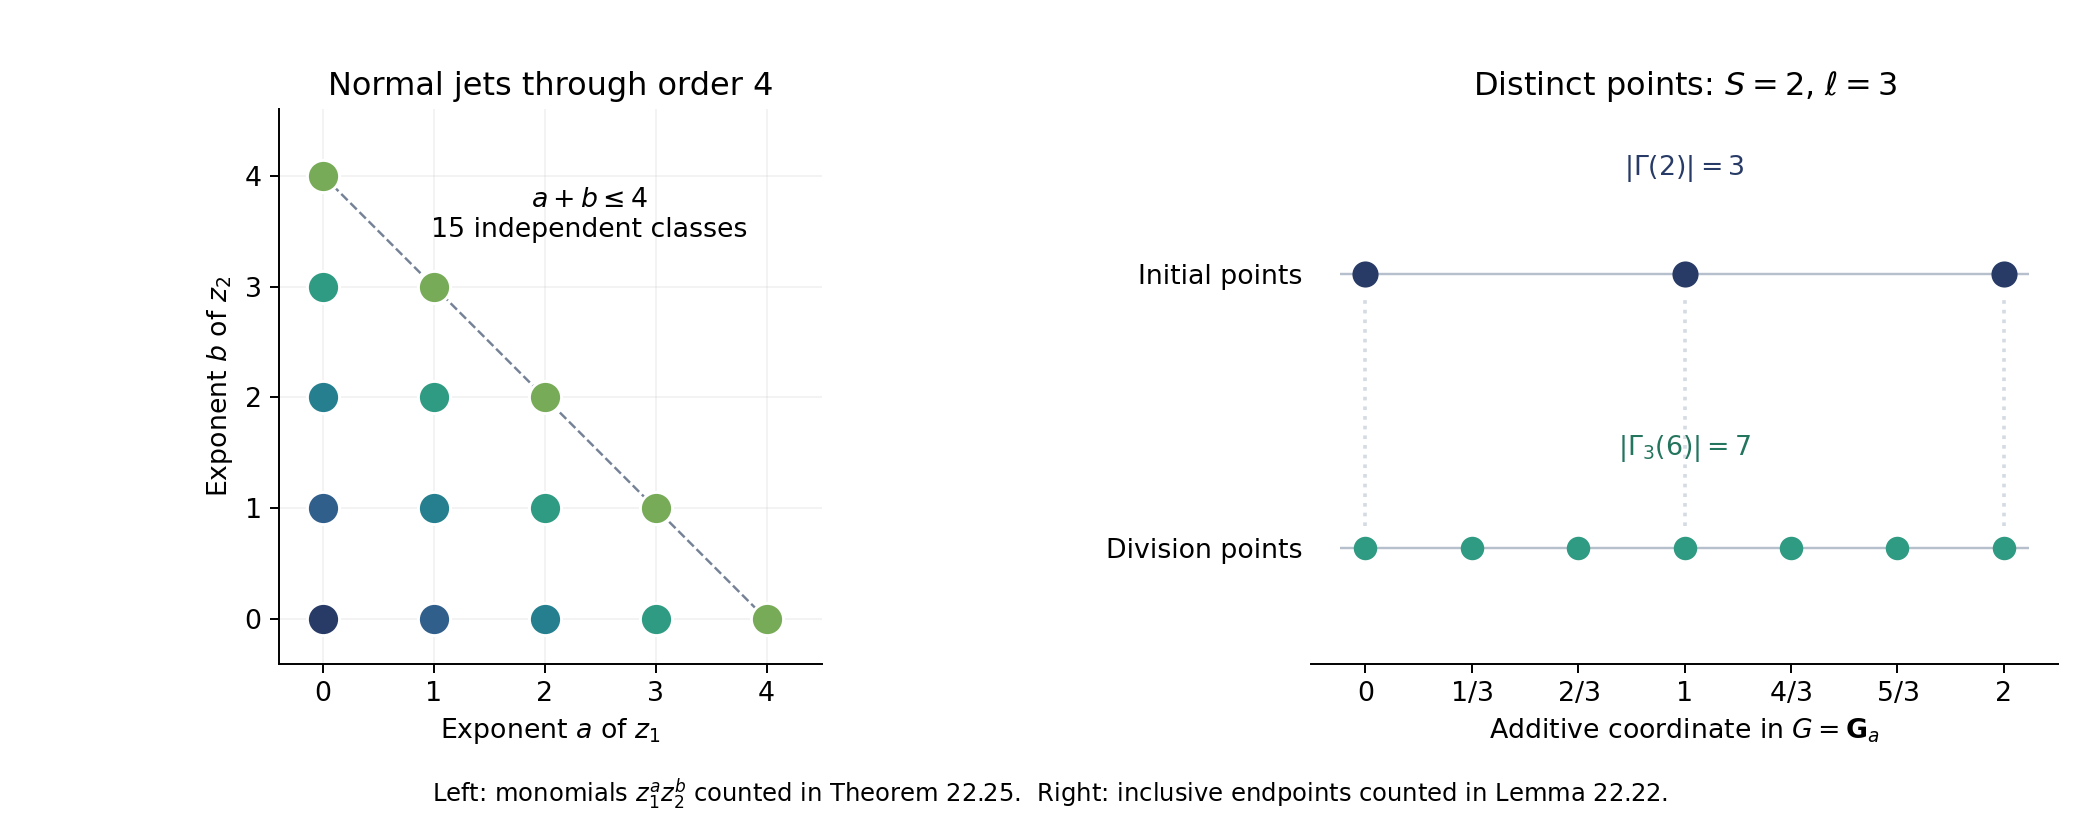
\includegraphics[keepaspectratio,alt={Transverse monomials and additive division points}]{../verification/lesson22/jets-and-division.png}}
\par\smallskip
\begin{flushleft}\small
\emph{Figure 22.1. The left panel lists the fifteen monomials of total
degree at most four in two normal variables, the sharp case of Theorem
22.25. The right panel shows the three points 0, 1, 2 and the seven
points 0, 1/3, 2/3, 1, 4/3, 5/3, 2 in the additive group, illustrating
the inclusive endpoint count in Lemma 22.22. Both panels depict exact
finite sets.
\href{verification/lesson22/jets-and-division.py}{Reproducible
figure}. The local multiplicity argument is developed above from the
method of
\href{https://archive.mpim-bonn.mpg.de/1364/1/preprint_1984_13.pdf}{Wüstholz}.}
\end{flushleft}
\end{minipage}\par\medskip


\subsection{From a tangent subvariety to an algebraic
subgroup}\label{from-a-tangent-subvariety-to-an-algebraic-subgroup}

For a hyperplane in the Lie algebra there is a direct geometric test for
the rank appearing in Corollary 22.26. Throughout this section
\(k\subset\mathbf C\) is algebraically closed of characteristic zero,
\(G/k\) is a connected commutative algebraic group of dimension \(n\),
and tangent spaces are identified with \(\operatorname{Lie}G\) by
translation. Smoothness of \(G\) is supplied by
\href{../AG-GS/AG-GS-02.html\#4-why-characteristic-zero-forces-smoothness}{Cartier's
theorem, Theorem 4.3 of \emph{Lie algebras and smoothness}}. We also use
the proved
\href{../AG-GS/AG-GS-03.html\#gs03-algebraically-closed-products}{product-domain
argument of \emph{Group schemes over a field}} and
\href{../AG-CA/AG-CA-18.html}{\emph{Smooth algebras over a field and
the Jacobian criterion}, Lemma 1.1, Theorem 2.1 and Corollary 2.2}.

\subsubsection{Proposition 22.27. Generating a subgroup inside a Lie
subspace}\label{proposition-22.27.-generating-a-subgroup-inside-a-lie-subspace}

Let \(W\subset\operatorname{Lie}G\) be a \(k\)-linear subspace. Suppose
\(V\subset G\) is a positive-dimensional irreducible closed
\(k\)-subvariety and, on a nonempty open subset of its smooth locus, \[
 T_vV\subset W
 \quad\text{after translation to the identity}.
 \tag{22.68}
\] There is a positive-dimensional connected closed algebraic subgroup
\(H\subset G\), defined over \(k\), such that \[
 \operatorname{Lie}H\subset W.
 \tag{22.69}
\]

\textbf{Proof.} We first explain a differential fact used in the
argument. For a dominant morphism \(X\to Y\) of irreducible varieties in
characteristic zero, its differential has rank \(\dim Y\) on a nonempty
open subset of the smooth loci. Choose a transcendence basis
\(t_1,\ldots,t_d\) of \(k(Y)/k\), and extend it to one of \(k(X)/k\). In
characteristic zero the remaining algebraic extensions of the rational
function fields are separable. Differentiation with respect to any
chosen basis element extends to a separable algebraic extension:
differentiating a minimal polynomial \(P(a)=0\) determines the
derivative of \(a\), since \(P'(a)\ne0\). Consequently
\(dt_1,\ldots,dt_d\) remain independent in the function field of \(X\).
This is the generic rank assertion. Clearing the finitely many
denominators and the nonzero minor gives the required open set. The
smooth loci are nonempty for these characteristic-zero varieties; the
same separating transcendence basis and Jacobian criterion give this
fact.

Consider the image \(X=V-V\) as a set, and let \(Z_j\) be the Zariski
closure of the image of \[
 V^{2j}\longrightarrow G,\qquad
 (v_1,w_1,\ldots,v_j,w_j)\longmapsto
       \sum_{i=1}^j(v_i-w_i),\qquad j\ge1.
 \tag{22.70}
\] Each \(Z_j\) is irreducible, is defined over \(k\), contains the
identity, and is invariant under inversion. The sets form an increasing
chain, because a further pair can be chosen equal. Also
\(\dim Z_1\ge\dim V>0\): fixing a point \(w\in V(k)\) puts the translate
\(V-w\) in \(Z_1\).

We claim that, at a general smooth point of every \(Z_j\), its
translated tangent space lies in \(W\). Use (22.70) as a dominant map
onto its image closure. At a general tuple of smooth points of \(V\),
its differential is the sum of the translated tangent vectors with the
indicated plus and minus signs. This follows by differentiating addition
and inversion; translation identifies the differential of addition with
vector addition in the Lie algebra of a commutative group. Hypothesis
(22.68) puts that image in \(W\). The differential fact just proved
makes it the entire tangent space of \(Z_j\) at a general image point,
proving the claim.

The dimensions of the increasing irreducible \(Z_j\) are bounded by
\(n\), so for some \(j\) they agree in two consecutive places. Then
\(Z_j=Z_{j+1}\). For \(x\in X\), translation gives
\(x+Z_j\subset Z_{j+1}=Z_j\); both sides are irreducible closed
subvarieties of equal dimension, so \(x+Z_j=Z_j\). Repeating this
equality shows that every element of the set \(jX\) stabilizes \(Z_j\).

For any fixed \(z\in Z_j\), the set \(\{g\in G:g+z\in Z_j\}\) is closed
and contains \(jX\). It therefore contains its closure \(Z_j\). Thus
\(Z_j+Z_j\subset Z_j\). We already know that \(-Z_j=Z_j\) and
\(0\in Z_j\). Hence \(H=Z_j\), with its reduced structure, is a closed
algebraic subgroup. It is connected because it is irreducible, and it
has positive dimension. Characteristic-zero smoothness and translation
now identify every tangent space of \(H\) with \(\operatorname{Lie}H\).
The claim about the generic tangent space yields (22.69). \(\square\)

\subsubsection{Corollary 22.28. Full normal rank when no subgroup lies
in a
hyperplane}\label{corollary-22.28.-full-normal-rank-when-no-subgroup-lies-in-a-hyperplane}

Suppose \(W\) is a hyperplane in \(\operatorname{Lie}G\) and contains
the Lie algebra of no positive-dimensional connected algebraic subgroup
defined over \(k\). Let \(V\subset G\) be an irreducible
\(k\)-subvariety of codimension \(r\), with \(1\le r<n\). For a basis
\(\Delta_1,\ldots,\Delta_{n-1}\) of the invariant derivatives associated
to \(W\), the matrix of derivatives of generators of the ideal of \(V\)
has generic rank \[
 \rho(V)=r.
 \tag{22.71}
\] For a point, of codimension \(n\), the rank is \(n-1\).

\textbf{Proof.} At a smooth point \(v\in V\), the differentials of
generators of its ideal have common kernel \(T_vV\); this is the
definition of the Zariski tangent space. Their restriction to \(W\)
consequently has rank \[
 \dim W-\dim(W\cap T_vV).
 \tag{22.72}
\] Since \(\dim T_vV=n-r\), this rank is \(r\) if \(T_vV\not\subset W\),
and \(r-1\) if \(T_vV\subset W\). Generic rank is well-defined: the
minors of a derivative matrix are regular functions on an affine open,
and its largest nonzero minor stays nonzero on a dense open subset. If
that generic rank were less than \(r\), Proposition 22.27 would produce
a positive-dimensional subgroup with Lie algebra in \(W\), a
contradiction. This proves (22.71). At a point, its tangent space as a
reduced subvariety is zero, so (22.72) is \(\dim W=n-1\). \(\square\)

Combined with Corollary 22.26, this gives a precise local obstruction.
Under the hypothesis of Corollary 22.28, a primary component supported
in codimension \(r<n\) that absorbs all derivatives through order \(T\)
has length at least \(\binom{T+r}{r}\). A component supported at a point
has length at least \(\binom{T+n-1}{n-1}\). Theorem 22.32 compares these
lengths with the degrees of the successive derivative ideals, using the
projective degree calculation in Lemmas 22.29--22.30.

\subsection{A global multiplicity estimate for a Lie
hyperplane}\label{a-global-multiplicity-estimate-for-a-lie-hyperplane}

We now turn the local length bound into a global estimate. The argument
needs a projective embedding on which the invariant derivatives extend
regularly. We state that geometric hypothesis explicitly. The estimate
proved here will apply to such an embedding once its construction and
its arithmetic properties have been supplied. Its constants depend on
the embedding and the chosen Lie directions, not on the polynomial or
the finite set of points.

The local-to-global method is developed in Wüstholz's freely accessible
\href{https://archive.mpim-bonn.mpg.de/1364/1/preprint_1984_13.pdf}{\emph{Multiplicity
Estimates on Group Varieties}, Sections 3--4}. For the hyperplane case,
Corollary 22.28 supplies full normal rank at every positive-dimensional
component. This permits the following direct construction by successive
derivatives.

\subsubsection{Lemma 22.29. Degree and the cycle of a
hypersurface}\label{lemma-22.29.-degree-and-the-cycle-of-a-hypersurface}

Let \(Y\subset\mathbf P^N_k\) be an integral projective variety of
dimension \(d\), over an algebraically closed field. Its degree is the
positive integer \(\deg Y\) defined by \[
 \dim_k A_t=\frac{\deg Y}{d!}t^d+O(t^{d-1}),
 \qquad A=k[X_0,\ldots,X_N]/I(Y),
 \tag{22.73}
\] for sufficiently large \(t\). When \(d=0\), the assertion means that
this Hilbert function is eventually the constant \(\deg Y\).

If \(d\ge1\) and a homogeneous form \(F\) of degree \(e\ge1\) is not
identically zero on \(Y\), then \[
 \sum_Z m_Z\deg Z=e\deg Y,
 \qquad
 m_Z=\operatorname{length}_{\mathcal O_{Y,\eta_Z}}
          \bigl(\mathcal O_{Y,\eta_Z}/(F)\bigr).
 \tag{22.74}
\] Here \(Z\) ranges over the irreducible components of \(Y\cap V(F)\),
and \((F)\) means any local trivialization of the homogeneous equation.

\textbf{Proof.} We use the proved
\href{../AG-CA/AG-CA-10.html}{Hilbert--Serre theorem, Theorem 3.1 of
\emph{Graded modules and Hilbert--Samuel functions}}, the
\href{../AG-CA/AG-CA-09.html}{dimension formula, Theorem 6.1 of
\emph{Krull dimension and Noether normalization}}, and the
\href{../AG-CA/AG-CA-11.html}{Hilbert--Samuel dimension theorem,
Corollary 2.2 of \emph{Dimension theory of Noetherian local rings}}. We
give the passage from those affine statements to (22.74).

Hilbert--Serre says that \(\dim_k A_t\) is eventually a polynomial. Put
\(\mathfrak m=A_{>0}\). Since \(A\) is generated in degree one,
\(A/\mathfrak m^s=\bigoplus_{t<s}A_t\). Localizing this quotient at
\(\mathfrak m\) does not change it: a denominator with nonzero constant
term has an inverse by a finite geometric series. Thus its vector-space
dimension is the Hilbert--Samuel function of \(A_{\mathfrak m}\). Its
degree is \(\dim A_{\mathfrak m}=\dim A=d+1\).

For completeness, the last equality follows on a nonempty chart
\(X_j\ne0\). The degree-zero part of \(A[X_j^{-1}]\) is the coordinate
ring of that chart, and \(A[X_j^{-1}]\) is that ring with the invertible
indeterminate \(X_j\) adjoined. Independence of powers of \(X_j\)
follows from the grading, after clearing homogeneous denominators. The
fraction field therefore has transcendence degree \(d+1\). Noether
normalization and the cited dimension formula give the asserted
dimensions, including the dimension at the closed vertex
\(\mathfrak m\).

Taking a first difference of the Hilbert--Samuel polynomial shows that
the Hilbert polynomial of \(A\) has degree \(d\) and positive leading
coefficient. Its \(d\)-th finite difference is a positive integer, since
the polynomial takes integer values at sufficiently large integers. This
proves (22.73) with \(\deg Y\) a positive integer.

We also need additivity with generic multiplicities. A finite graded
module over a Noetherian graded ring has a filtration with factors
\((A/\mathfrak p)(b)\), for homogeneous primes \(\mathfrak p\) and
grading shifts \(b\). Here is the usual filtration argument in this
setting. Choose a nonzero homogeneous element whose annihilator is
maximal among annihilators of nonzero homogeneous elements. Its
homogeneous annihilator is prime: for homogeneous \(a,b\), if \(ab\)
annihilates the element and \(b\) does not, maximality applied to the
element multiplied by \(b\) forces \(a\) into the annihilator. A
homogeneous ideal with this property is prime, as is seen by taking the
first nonzero homogeneous terms of two products in its graded quotient.
The generated cyclic submodule gives one factor. Repeat in the graded
quotient; the ascending chain condition on submodules makes the process
terminate.

Hilbert functions add in these exact sequences. Grading shifts do not
change leading coefficients. Among the factors of largest support
dimension, the number with a given minimal prime \(\mathfrak p\) is the
length of the original module localized at \(\mathfrak p\): localizing
the filtration kills every other factor, and the surviving factors are
its residue field. Thus the leading coefficient is the sum of the
component degrees weighted by these generic lengths. The same
observation on an affine projective chart identifies the cone
multiplicity with the local length on the projective component:
adjoining and inverting the grading variable only extends the generic
residue field and leaves the length unchanged.

Multiplication by \(F\) is injective in the domain \(A\). Consequently
the exact sequence \[
 0\longrightarrow A(-e)\xrightarrow{\ F\ }A
   \longrightarrow A/(F)\longrightarrow0
 \tag{22.75}
\] gives the Hilbert polynomial \(h_A(t)-h_A(t-e)\), with leading term
\(e\deg Y\,t^{d-1}/(d-1)!\). The principal ideal theorem and the
finite-type dimension formula show that every minimal component of the
hypersurface has dimension \(d-1\). The leading-coefficient additivity
just proved now gives exactly (22.74). Embedded components of smaller
dimension have no contribution to that coefficient. \(\square\)

\subsubsection{Lemma 22.30. A degree bound on a smooth open
subset}\label{lemma-22.30.-a-degree-bound-on-a-smooth-open-subset}

Let \(U\) be a smooth dense open subset of an integral projective
variety \(X\subset\mathbf P^N_k\) of dimension \(n\) and degree
\(\delta\). Let \(Q_1,\ldots,Q_r\) be homogeneous forms of positive
degrees \(e_1,\ldots,e_r\). Suppose their successive zero schemes on
\(U\) are cut out by regular sequences, and \(Q_{i+1}\) vanishes
identically on no irreducible component of the preceding zero scheme.
Then every component of the final zero scheme has codimension \(r\) in
\(U\), and \[
 \sum_V\lambda_V\deg\overline V
       \le\delta\prod_{i=1}^r e_i,
 \qquad
 \lambda_V=\operatorname{length}_{\mathcal O_{U,\eta_V}}
    \bigl(\mathcal O_{U,\eta_V}/(Q_1,\ldots,Q_r)\bigr).
 \tag{22.76}
\] The closures are taken in \(X\). In particular, for \(r=n\) the sum
of the lengths at all remaining points is at most the right side.

\textbf{Proof.} The needed commutative algebra is
\href{../AG-CA/AG-CA-12.html}{\emph{Regular sequences, depth and
Cohen--Macaulay modules}, Theorems 4.1, 5.1 and 6.1 and Corollary 6.2}:
regular local rings are Cohen--Macaulay, their regular-sequence
quotients are Cohen--Macaulay, and such quotients have no embedded
associated primes. Together with the dimension formula, these results
give the codimension assertion.

We justify the multiplicities in the induction, rather than assuming
that the projective closure is itself a complete intersection. Let \(Y\)
be a new component after adjoining the next equation \(f\), and work at
its generic point. If \(R=\mathcal O_{U,\eta_Y}\) and \(J\) is the
preceding ideal, then \(M=R/J\) is a one-dimensional Cohen--Macaulay
module and \(f\) is a nonzerodivisor on it. Moreover \(M/fM\) has finite
length. For any subquotient \(N\) of \(M\), both the kernel and cokernel
of multiplication by \(f\) have finite length. Indeed, away from the
maximal ideal of \(R\), every point of its support is a minimal point of
\(\operatorname{Supp}M\), and \(f\) is invertible there.

Define \[
 \chi_f(N)=\operatorname{length}(N/fN)
                   -\operatorname{length}(0:_N f).
 \tag{22.77}
\] The kernel--cokernel exact sequence for multiplication by \(f\) in a
short exact sequence shows that \(\chi_f\) is additive. A finite-length
module has \(\chi_f=0\), because an endomorphism of such a module has
kernel and cokernel of equal length. Apply a prime filtration of \(M\),
constructed by the maximal-annihilator argument used above without
gradings. Its one-dimensional factors are \(R/\mathfrak p\) for the
minimal primes of \(M\); all other factors have finite length. On a
one-dimensional domain factor, the kernel of \(f\) is zero. Localization
of the filtration counts its occurrences. Hence \[
 \operatorname{length}(M/fM)
   =\sum_{\mathfrak p\in\operatorname{Min}M}
       \operatorname{length}(M_{\mathfrak p})
       \operatorname{length}\bigl(R/(\mathfrak p,f)\bigr).
 \tag{22.78}
\] The last factors are precisely the generic intersection
multiplicities of the preceding reduced components with the
hypersurface.

Apply Lemma 22.29 to the projective closure of each preceding component,
with its weight \(\lambda_V\). Equation (22.78) identifies the resulting
weights at every new component meeting \(U\). Components contained in
\(X\setminus U\) have nonnegative degrees and weights and can be omitted
from an upper bound. Each step therefore multiplies the upper bound by
at most the degree of the new equation. Starting with \([X]\) proves
(22.76). At a closed point over \(k\), the projective degree is one,
which gives the last assertion. \(\square\)

\subsubsection{Lemma 22.31. Homogeneous derivatives with controlled
degree}\label{lemma-22.31.-homogeneous-derivatives-with-controlled-degree}

Let \(X\subset\mathbf P^N_k\) be integral and let \(\Delta\) be a
regular vector field on \(X\). On each nonempty standard affine chart
\(X_j\ne0\), choose polynomial representatives \[
 \Delta(X_l/X_j)=P_{j,l}(X/X_j)\quad(l\ne j),
 \qquad \deg P_{j,l}\le a,
 \qquad a\ge2.
 \tag{22.79}
\] There is a common such integer \(a\) for any fixed finite family of
vector fields. If \(Q\) is homogeneous of degree \(e\), put \[
 \mathcal D_{j,e}Q
   =\sum_{l\ne j}X_j^aP_{j,l}(X/X_j)
                       \frac{\partial Q}{\partial X_l}.
 \tag{22.80}
\] This is a homogeneous polynomial of degree \(e+a-1\), and on the
\(j\)-th chart its dehomogenization is \(\Delta(Q/X_j^e)\). On any other
chart \(X_h\ne0\), write \(\xi=X_j/X_h\) and \(q=Q/X_h^e\). Then \[
 \frac{\mathcal D_{j,e}Q}{X_h^{e+a-1}}
  =\xi^{a-1}\Delta q-e\xi^{a-2}(\Delta\xi)q.
 \tag{22.81}
\] In particular, if \(\Delta\) is an invariant direction in \(W\),
applying (22.80) lowers order of vanishing along \(W\) by at most one at
every point of \(G\subset X\), including points where \(X_j=0\). A word
of length \(t\) gives degree \(e+(a-1)t\) and order loss at most \(t\).

\textbf{Proof.} A vector field acts as a derivation on the coordinate
ring of every affine chart. That ring is a quotient of a polynomial ring
in the ratios \(X_l/X_j\), so representatives \(P_{j,l}\) exist. There
are only finitely many charts and vector fields; increase their degree
bound to an integer \(a\ge2\).

Each \(X_j^aP_{j,l}(X/X_j)\) is a homogeneous polynomial of degree
\(a\), so (22.80) has the stated degree. The chain rule on the \(j\)-th
chart gives its first assertion. On the overlap with the \(h\)-th chart
its normalization is \(\xi^{e+a-1}\Delta(q/\xi^e)\); the product rule
gives (22.81). Both coefficients on the right are regular on the entire
\(h\)-th chart because \(a\ge2\) and \(\Delta\) is regular on \(X\).
Thus the identity extends from the overlap to the whole chart. If a
coordinate \(X_j\) is identically zero on \(X\), its empty chart is
simply unused.

Order along \(W\) means that all words in the invariant derivatives of
length less than that order vanish at the point. Differentiation in a
direction of \(W\) lowers it by at most one. Multiplication by any
regular function does not lower it, by the iterated product rule.
Formula (22.81) proves the assertion at all points. Iteration uses the
updated homogeneous degree at each step. On the chosen \(j\)-th chart,
it gives exactly the corresponding word of derivatives of the original
dehomogenization. \(\square\)

\subsubsection{Theorem 22.32. The hyperplane multiplicity
estimate}\label{theorem-22.32.-the-hyperplane-multiplicity-estimate}

Let \(k\subset\mathbf C\) be algebraically closed, and let \(G/k\) be a
connected commutative algebraic group of dimension \(n\ge2\). Suppose
\(G\) is a dense open subset of an integral projective variety
\(X\subset\mathbf P^N_k\) of degree \(\delta\). Let
\(W\subset\operatorname{Lie}G\) be a hyperplane whose invariant vector
fields extend regularly to \(X\). Suppose \(W\) contains the Lie algebra
of no positive-dimensional connected algebraic subgroup over \(k\).

Choose a basis of \(W\), and let \(a\ge2\) be a common bound as in Lemma
22.31. The following positive integers depend only on these fixed data:
\[
 \begin{split}
 c_1&=1,\qquad B_r=\delta\prod_{i=1}^r c_i,\qquad
 K_r=r!B_r+1,\qquad
 c_{r+1}=c_r+(a-1)K_r\quad(1\le r<n),\\
 L&=\sum_{r=1}^{n-1}K_r,\qquad
 C_{\mathrm{mult}}=2^{n-1}(n-1)!B_n.
 \end{split}
 \tag{22.82}
\] Let \(P\) be a homogeneous form of degree \(D\ge1\) that is not
identically zero on \(G\), and let \(\Sigma\subset G(k)\) be finite. If
\(P\) vanishes along \(W\) to order at least an integer \(T\) at every
point of \(\Sigma\), and \(T\ge2LD\), then \[
                    |\Sigma|T^{n-1}\le C_{\mathrm{mult}}D^n.
 \tag{22.83}
\]

\textbf{Proof.} The case \(\Sigma=\varnothing\) is immediate, so assume
it is nonempty. We construct homogeneous forms \(Q_1=P,Q_2,\ldots,Q_n\),
with \(\deg Q_i=c_iD\). On \(G\), their successive ideals \(J_r\) will
define nonempty complete intersections of pure codimension \(r\). Every
generator of \(J_r\) will have order at least \[
                   T-D\sum_{h<r}K_h
 \tag{22.84}
\] along \(W\) at \(\Sigma\). The first step holds because \(G\) is
smooth and integral and \(P\) is nonzero on it. Lemma 22.30 gives, at
every step already constructed, \[
        \sum_{V\in\operatorname{Irr}V(J_r)}
                 \lambda_V\deg\overline V\le B_rD^r.
 \tag{22.85}
\]

Suppose \(r<n\) and fix one of these components \(V\). Its positive
dimension and Corollary 22.28 imply that the invariant derivatives in
\(W\) have full normal rank \(r\) at its generic point. Work on a
standard chart meeting \(V\), then localize at that generic point. The
ideal \(J_r\) becomes primary for the maximal ideal of this local ring;
its quotient has length \(\lambda_V\le B_rD^r\), because
\(\deg\overline V\ge1\).

Put \(t_r=K_rD\). The choice (22.82) gives \[
 \binom{t_r+r}{r}\ge\frac{t_r^r}{r!}>B_rD^r\ge\lambda_V.
 \tag{22.86}
\] If every derivative of every dehomogenized generator of \(J_r\),
through order \(t_r\), belonged to the prime ideal of \(V\), the
localization and product-rule argument of Lemma 22.24 would give the
same assertion for every element of the localized ideal. Normalize an
invertible \(r\times r\) minor of the normal derivative matrix, exactly
as in Corollary 22.26. Theorem 22.25 would force its length to be at
least \(\binom{t_r+r}{r}\), contradicting (22.86). Therefore some word
of at most \(t_r\) derivatives of one generator is nonzero at the
generic point of \(V\).

Apply the homogeneous operators of Lemma 22.31 on that chart. The
resulting polynomial \(R_V\) does not vanish identically on \(V\), has
degree at most \(c_rD+(a-1)t_r=c_{r+1}D\), and has order at least
(22.84) minus \(t_r\) at every point of \(\Sigma\). The assertion about
all points, even those outside the chosen chart, is exactly the reason
for formula (22.81).

There are finitely many components. Choose a linear form \(H\) nonzero
at every one of their generic points. Such a form exists: each forbidden
condition is a proper linear subspace of the finite-dimensional space of
linear forms, and a finite union of proper linear subspaces over an
infinite field cannot cover that space. To see the last fact, choose a
nonzero linear functional vanishing on each subspace. Their product is a
nonzero polynomial; induction on the number of variables shows that a
nonzero polynomial over an infinite field cannot vanish at every point.

Multiply each \(R_V\) by the needed power of \(H\) to give it degree
\(c_{r+1}D\). This preserves its nonvanishing on \(V\) and its lower
bound for order at \(\Sigma\). A linear combination of the resulting
finitely many polynomials can be chosen nonzero on every component: for
each component, the coefficients giving zero in its function field form
a proper linear subspace, since its own \(R_V\) is nonzero. The same
finite-subspace argument applies. Call the chosen combination
\(Q_{r+1}\).

The preceding complete intersection is Cohen--Macaulay and has no
embedded associated primes. Avoiding its irreducible components
therefore makes \(Q_{r+1}\) a nonzerodivisor wherever its new zero
scheme is nonempty. The cited regular-sequence results and dimension
formula give pure codimension \(r+1\). Its order at \(\Sigma\) is at
least \(T-D\sum_{h\le r}K_h\), so it still contains \(\Sigma\): this
integer is at least \(T-LD\ge T/2\ge1\). Lemma 22.30 supplies (22.85)
for the new ideal. This completes the induction.

The zero scheme of \(J_n\) on \(G\) is finite. Set \(T_0=T-LD\). At
\(s\in\Sigma\), every word of length at most \(T_0-1\) sends every
element of \((J_n)_s\) into the maximal ideal; use (22.84) and the
product rule, including localization. The normal rank at a point is
\(n-1\). Theorem 22.25 and the same normalization of a nonzero minor
give \[
 \operatorname{length}_{\mathcal O_{G,s}}
            \bigl(\mathcal O_{G,s}/(J_n)_s\bigr)
 \ge\binom{T_0+n-2}{n-1}
 \ge\frac{T_0^{n-1}}{(n-1)!}
 \ge\frac{T^{n-1}}{2^{n-1}(n-1)!}.
 \tag{22.87}
\] Sum this inequality over \(\Sigma\), and bound the sum of all point
lengths by \(B_nD^n\) using (22.85). This is (22.83). \(\square\)

\subsubsection{Corollary 22.33. The geometric contradiction after
extrapolation}\label{corollary-22.33.-the-geometric-contradiction-after-extrapolation}

Use the notation of Proposition 22.21: \(n\ge2\), \(m\ge1\), \(k\ge5\),
\(S=\ell^{2n+1}\), \(1\le q\le S+1\), \(A=2nmqS^{nk}\), and \(D=A/S^k\).
Suppose the hypotheses on \(G,X,W\) in Theorem 22.32 hold. Suppose a
nonzero form of degree \(D\) has order at least an integer \(T'\ge A/8\)
along \(W\) at a set of at least \(\ell q/2\) distinct division points.
These conditions are impossible when \[
 S^k\ge16L,
 \qquad
 \ell>4nm\,8^{n-1}C_{\mathrm{mult}}.
 \tag{22.88}
\]

\textbf{Proof.} First \(T'/D\ge S^k/8\ge2L\). Furthermore \[
 \frac{|\Sigma|(T')^{n-1}}{D^n}
 \ge\frac{\ell q}{2}\frac{(A/8)^{n-1}}{(A/S^k)^n}
 =\frac{\ell}{4nm\,8^{n-1}}
 >C_{\mathrm{mult}},
 \tag{22.89}
\] contradicting (22.83). \(\square\)

Theorem 22.45 supplies the group compactification with regular invariant
fields, and Theorem 22.43 supplies the division-field degree. The height
and denominator estimates are proved in22.47--56, the normalized entire
lift and its jet estimates in22.58--61, and the auxiliary-section
construction in22.62. Theorem22.63 combines these with the multiplicity
estimate, retaining the dyadic torsion factor from Lemma22.53.

\subsubsection{Example 22.34. A derivative cut and its point at
infinity}\label{example-22.34.-a-derivative-cut-and-its-point-at-infinity}

Take \(G=\mathbf G_a\times\mathbf G_m\), with coordinates \((x,y)\), and
the invariant derivative \(\Delta=\partial_x+y\partial_y\). Its Lie line
contains no positive-dimensional algebraic subgroup, by the
classification in Theorem 22.4. The Segre compactification is \[
 (x,y)\longmapsto[1:x:y:xy],\qquad
 X_0X_3-X_1X_2=0\quad\text{in }\mathbf P^3.
 \tag{22.90}
\] Its degree is two: the exact sequence for its single quadratic
equation in the polynomial ring gives Hilbert function
\(\binom{t+3}{3}-\binom{t+1}{3}=(t+1)^2\).

Let \(F=y-1-x\). Then \(\Delta F=y-1\), so their common zero on \(G\) is
\((0,1)\), with length one: the ideal \((y-1-x,y-1)\) is \((x,y-1)\). On
the analytic curve \((x,y)=(t,e^t)\), the function \(F\) has order two
at zero, since \(F(0)=F'(0)=0\) and \(F''(0)=1\). Thus the derivative
cuts the curve even though the original curve and the Lie direction are
tangent at that point.

The two affine equations have the linear homogeneous extensions
\(F_h=X_2-X_0-X_1\) and \(H_h=X_2-X_0\). Their intersection on the
quadric consists of \[
       [1:0:1:0]\quad\text{and}\quad[0:0:0:1].
 \tag{22.91}
\] Indeed, subtracting the equations gives \(X_1=0\), then \(X_2=X_0\),
and the quadric equation becomes \(X_0X_3=0\). The first point is the
affine point already found. For the second, use the chart \(X_3=1\),
with \(p=X_1/X_3\), \(q=X_2/X_3\), so \(X_0=pq\). The equations become
\(q-pq-p\) and \(q-pq\). Their difference gives \(p\), and the second
then gives \(q\); the quotient again has length one. This point is
outside \(G\). Thus the projective degree count is \(2=1+1\), while the
sum retained on \(G\) is only one, exactly as in Lemma 22.30.

\begin{minipage}[t]{\linewidth}
\centering
\pandocbounded{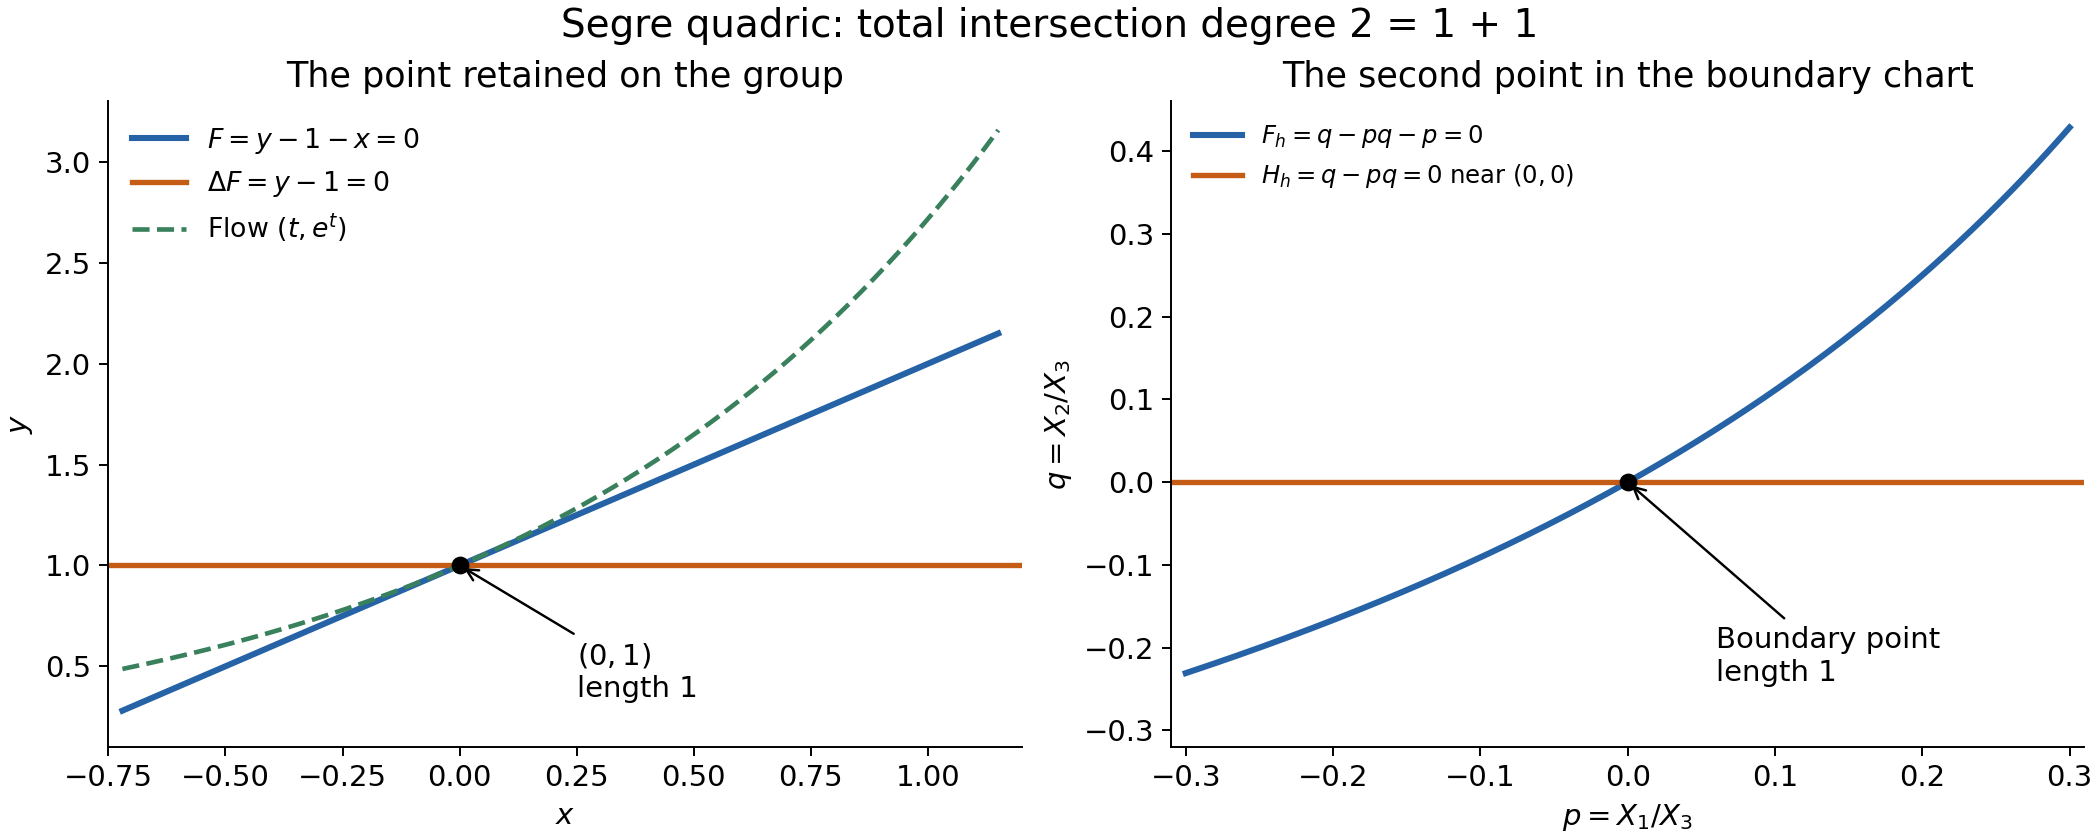
\includegraphics[keepaspectratio,alt={The derivative cuts the curve at (0,1); a second simple intersection lies in the chart at infinity.}]{../verification/lesson22/multiplicity-cuts.png}}
\par\smallskip
\begin{flushleft}\small
\emph{Figure 22.2. Exact equations from Example 22.34, drawn on real
slices of the two affine charts. Left: \(F=0\), \(\Delta F=0\), and the
analytic flow \((t,e^t)\). Right: near the boundary point, \(F_h=0\) is
\(q=p/(1-p)\) and \(H_h=0\) is \(q=0\). Each marked point has algebraic
intersection length one. The picture represents these chart slices; the
degree calculation is the algebraic computation above. }
\end{flushleft}
\end{minipage}\par\medskip


\subsection{Period lattices and the field of a division
point}\label{period-lattices-and-the-field-of-a-division-point}

The division-field bound used in extrapolation has a direct explanation
in terms of the exponential kernel. It does not require a bound on the
coefficients of the multiplication map. We distinguish analytic
connectedness, used for the exponential, from the algebraic statements
about its finite fibres.

\subsubsection{Proposition 22.35. The exponential of a connected
commutative complex Lie
group}\label{proposition-22.35.-the-exponential-of-a-connected-commutative-complex-lie-group}

Let \(H\) be a connected commutative complex Lie group of complex
dimension \(n\). Its exponential is a surjective holomorphic
homomorphism \[
 \exp_H:\mathbf C^n\longrightarrow H,
 \qquad H\simeq\mathbf C^n/\Lambda,
 \qquad \Lambda\simeq\mathbf Z^r,
 \qquad 0\le r\le2n.
 \tag{22.92}
\] The chosen identification of the tangent space with \(\mathbf C^n\)
is the only choice in this notation. The kernel \(\Lambda\) is discrete.
For every positive integer \(b\), multiplication by \(b\) is surjective
and each of its fibres has exactly \(b^r\) points.

\textbf{Proof.} The parameter-dependent flow and exponential
construction are proved for arbitrary real Lie groups in
\href{../DG-FND/local-tools-for-bundles-and-transport.html\#2-differential-equations-and-their-parameters}{\emph{Local
tools for bundles and transport}, Theorem 2.1, Lemma 2.2 and Proposition
2.3}. In particular invariant vector fields have solutions on every
finite time interval, by translating a single identity chart and
restarting a bounded number of times. Compactness is not required.

Apply that construction to the underlying real group. Let
\(\gamma_v(t)\) be the identity-starting solution with invariant initial
velocity \(v\). The differential of addition, after translating tangent
spaces to the identity, is vector addition. Thus
\(\gamma_v(t)+\gamma_w(t)\) solves the same invariant equation as
\(\gamma_{v+w}(t)\). Uniqueness makes the curves equal. At time one this
proves that \(E(v)=\gamma_v(1)\) is a homomorphism. The cited
smooth-dependence theorem and time rescaling give
\(dE_0=\operatorname{id}\). Differentiating the homomorphism identity
yields \(dE_v=dL_{E(v)}\circ dE_0\). These derivatives are
complex-linear, because translations in a complex Lie group are
holomorphic. Therefore the smooth map \(E\) is holomorphic. It is a
local biholomorphism at zero and, by translation, everywhere.

Its image is an open subgroup. The complement, being a union of other
open cosets, is open as well. Connectedness makes the image all of
\(H\). Local injectivity gives discreteness of \(\Lambda=\ker E\). The
homomorphism consequently induces a bijection
\(\mathbf C^n/\Lambda\to H\). A small ball whose difference set meets
\(\Lambda\) only at zero supplies quotient charts; the bijection and its
inverse are holomorphic in these charts, proving the analytic
isomorphism.

The elementary discrete-subgroup theorem, proved as
\href{https://github.com/KokunoYumeto/open-math-courses-public/blob/146dc81802e69cf262fb6cc65c1b9f74e71f4625/docs/courses/AG-GS/src/abelian-varieties.md}{Lemma
6.22 of \emph{Abelian varieties}}, applies to any finite-dimensional
real vector space, without a compact quotient hypothesis. It gives a
real-linearly independent integral basis of \(\Lambda\). Its size \(r\)
is at most the real dimension \(2n\). One can see the finiteness step
directly: select real-linearly independent elements spanning \(\Lambda\)
over \(\mathbf R\); their compact fundamental parallelepiped contains
only finitely many lattice points, by uniform separation of distinct
points of a discrete subgroup. The full subgroup is therefore a finite
extension of the subgroup they generate; the integer subgroup-basis
argument in that lemma gives the asserted free basis.

For \(h=E(v)\), the point \(E(v/b)\) maps to \(h\) under multiplication
by \(b\). Its fibre is a translate of the kernel. The map
\(\Lambda/b\Lambda\to H[b]\), \(\lambda\mapsto E(\lambda/b)\), is a
bijection: its kernel is \(b\Lambda\), and any \(E(w)\in H[b]\) has
\(bw\in\Lambda\). This quotient has \(b^r\) elements in a lattice basis.
\(\square\)

\subsubsection{Corollary 22.36. Division-field
degree}\label{corollary-22.36.-division-field-degree}

Let \(G\) be a smooth commutative algebraic group of dimension \(n\)
over a number field \(K\subset\mathbf C\), and suppose \(G(\mathbf C)\)
is connected in its analytic topology. Let \(\gamma\in G(K)\), and let
\(\eta\in G(\mathbf C)\) satisfy \([b]\eta=\gamma\), with \(b\ge1\).
Then \(\eta\) is algebraic over \(K\), and \[
 [K(\eta):K]\le b^r\le b^{2n},
 \qquad
 [K(\eta):\mathbf Q]\le[K:\mathbf Q]b^{2n},
 \tag{22.93}
\] where \(r\) is the rank of the exponential kernel in Proposition
22.35. All integer multiples of \(\eta\) are defined over the same field
\(K(\eta)\).

\textbf{Proof.} The differential of \([b]\), translated to the identity,
is multiplication by \(b\) on the tangent space: differentiate the sum
of \(b\) copies of the variable. It is invertible in characteristic
zero. Therefore the tangent space of each geometric fibre of \([b]\) is
zero. A local ring at a geometric point of such a fibre is Noetherian
and has \(\mathfrak m/\mathfrak m^2=0\); Nakayama gives
\(\mathfrak m=0\). In particular the finite-type fibre is
zero-dimensional and reduced. A finite-type zero-dimensional scheme over
a field is a finite disjoint union of spectra of finite field
extensions: cover it by finitely many affine opens, use the
zero-dimensional Noetherian-ring theorem and the field case of the
Nullstellensatz, and note that its finitely many points are open. The
needed results are proved in
\href{../AG-CA/AG-CA-03.html}{\emph{Noetherian and Artinian rings}}
and \href{../AG-CA/AG-CA-06.html}{\emph{The Nullstellensatz and
Jacobson rings}}.

Apply this to the fibre over the \(K\)-rational point \(\gamma\). Every
complex point of the fibre is therefore algebraic over \(K\). Its degree
\([K(\eta):K]\) is the number of its distinct conjugate geometric
points, since number fields have characteristic zero. Proposition 22.35
counts the entire fibre as \(b^r\) points, so the degree cannot exceed
that number. The absolute-degree bound follows from the tower formula.
Finally every multiplication-by-an-integer morphism is defined over
\(K\); applying it to a \(K(\eta)\)-point keeps its coordinates in that
field. \(\square\)

For the division point \(\eta=\exp_G(u/\ell)\) in Lemma 22.22, formula
(22.93) supplies the factor \(\ell^{2n}\) in the field-degree part of
the norm estimate. Theorem 22.42 below proves analytic connectedness for
irreducible complex varieties; Corollary 22.43 therefore supplies this
division-field bound for every smooth geometrically connected
commutative algebraic group. Bounds for heights, denominators and
homogeneous normalization remain distinct inputs.

\subsection{Affine factors and a compactification over an abelian
variety}\label{affine-factors-and-a-compactification-over-an-abelian-variety}

The zero estimate in Theorem 22.32 needs a projective ambient variety on
which the invariant vector fields are regular. An arbitrary projective
closure does not supply that property. We first describe the affine
factors of a commutative group, then construct an ambient variety from
an extension by those factors. Throughout this section
\(k=\overline{\mathbf Q}\subset\mathbf C\). A vector subgroup means a
linear subspace with its additive group law.

\subsubsection{Proposition 22.37. Several additive
coordinates}\label{proposition-22.37.-several-additive-coordinates}

Let \(W\subset\mathbf C^u\times\mathbf C^v\) be a complex linear
subspace. Write its coordinate projections as \(p:W\to\mathbf C^u\) and
\(z:W\to\mathbf C^v\). Put \[
 V=p(W),\qquad
 L=\{m\in\mathbf Z^v:m\cdot z(w)=0\text{ for every }w\in W\}.
 \tag{22.94}
\] Then \(L\) is saturated and \[
 \overline{\{(p(w),e^{z_1(w)},\ldots,e^{z_v(w)}):w\in W\}}^{\rm Zar}
       =V\times T_L.
 \tag{22.95}
\] Consequently every connected closed algebraic subgroup of
\(\mathbf G_a^u\times\mathbf G_m^v\) is the product of a vector subgroup
and a subtorus. When the subgroup is defined over \(k\), both factors
and their product decomposition are defined over \(k\).

\textbf{Proof.} Saturation follows by dividing a vanishing linear form
by a nonzero integer. A regular function on the ambient group has the
finite Laurent expansion \[
 F(x,y)=\sum_m P_m(x)y^m.
\] Group its terms by the cosets \(c\) of \(L\) that meet the support,
and write \(P_c=\sum_{m\in c}P_m\). The linear forms \(m\cdot z|_W\),
one for each such coset, are distinct; call them \(\lambda_c\). Suppose
\(F\) vanishes on the exponential image. Choose \(a\in W\) on which the
finitely many \(\lambda_c\) have distinct values. Such a choice exists
by the finite-hyperplane argument following Lemma 22.1. If there is only
one coset, any \(a\), including zero, suffices. For every fixed
\(b\in W\), substitution of \(w=b+ta\) gives \[
 \sum_c e^{\lambda_c(b)}P_c(p(b)+t p(a))e^{t\lambda_c(a)}=0
       \qquad(t\in\mathbf C).
\] Lemma 22.1 implies that every polynomial coefficient in \(t\)
vanishes. Setting \(t=0\) gives \(P_c(p(b))=0\) for all \(b\), hence
\(P_c|_V=0\). This argument includes \(W=0\): there is a single coset
and the assertion is evaluation at the identity.

Conversely those restrictions imply that \(F\) vanishes on the
exponential image. They also say precisely that \(F\) vanishes on
\(V\times T_L\). Indeed, after quotienting the polynomial ring by the
linear ideal of \(V\), the monomial-coordinate change in Lemma 22.2
makes the Laurent monomials indexed by distinct cosets a basis over
\(\mathbf C[V]\). Thus the vanishing ideals of the two sets agree,
proving (22.95).

Now let \(H\) be a connected closed subgroup over \(\mathbf C\), and
take \(W=\operatorname{Lie}H\). We justify the inclusion of its
exponential image without assuming that \(H(\mathbf C)\) is analytically
connected. For \(w=(a,z)\in W\), the ambient invariant derivation is \[
 D_w=\sum_{i=1}^u a_i\partial_{x_i}
           +\sum_{j=1}^v z_jy_j\partial_{y_j}.
\] Its tangent vector at every point of \(H\) is tangent to \(H\), by
translation. The defining ideal of the smooth reduced group \(H\) is
therefore preserved by \(D_w\): the derivative of a function vanishing
on \(H\) is zero at every point of \(H\), and the Nullstellensatz puts
it back in that ideal. All iterates have the same property. The entire
function \(t\mapsto F(ta,e^{tz})\), for \(F\) in this ideal, has all
Taylor coefficients zero at the origin. Hence it is identically zero,
proving \(\exp(W)\subset H\).

Let \(Z\) be the closure in (22.95). It is smooth, connected and
contained in \(H\). The exponential curves give
\(W\subset\operatorname{Lie}Z\), while the inclusion \(Z\subset H\)
gives the reverse inclusion. Smoothness makes their dimensions equal.
Since \(H\) is irreducible, by the programme group-component theorem
used before Lemma 22.1, a closed subset of the same dimension must equal
\(H\). This proves the product classification over \(\mathbf C\).

If \(H\) is defined over \(k\), then \(W=W_k\otimes_k\mathbf C\) for its
\(k\)-Lie algebra, and \(V\) is the scalar extension of the \(k\)-linear
image of \(W_k\). The lattice \(L\) is defined by integer equations and
the same linear tests on \(W_k\). Both factors therefore descend to
\(k\). Equality of their defining ideals with the ideal of \(H\) follows
from the equality over \(\mathbf C\), since scalar extension by a field
is faithfully flat. \(\square\)

\subsubsection{Theorem 22.38. A connected commutative affine group
splits}\label{theorem-22.38.-a-connected-commutative-affine-group-splits}

Every connected commutative affine algebraic group \(L_0\) over \(k\) is
isomorphic over \(k\) to \[
 L_0\simeq\mathbf G_a^a\times\mathbf G_m^b
 \tag{22.96}
\] for some nonnegative integers \(a,b\).

\textbf{Proof.} The faithful representation theorem, proved in
\href{../AG-GS/AG-GS-01.html\#5-why-affine-groups-over-a-field-are-matrix-groups}{\emph{Group
schemes, actions and Hopf algebras}, Theorem 5.2}, supplies a closed
embedding \(L_0\hookrightarrow\operatorname{GL}_N\). Its proof takes a
finite-dimensional subcomodule of the coordinate algebra containing a
set of algebra generators; the matrix coefficients then generate that
algebra, so the representation is a closed embedding, not merely
injective on points.

Let \(R\subset\operatorname{Mat}_N(k)\) be the unital \(k\)-algebra
generated by \(L_0(k)\). It is finite-dimensional and commutative.
Commutativity follows from the group law, and finite dimension follows
from the ambient matrix space. Every element of \(R\) which is
invertible as a matrix has its inverse in \(R\), by its characteristic
polynomial with nonzero constant term. Consequently
\(R^\times=R\cap\operatorname{GL}_N\), and \(L_0\) is a closed subgroup
of this unit group. These are scheme-theoretic inclusions: all groups in
characteristic zero are reduced, and their algebraically closed field
points are dense, so the linear equations defining \(R\) vanish on
\(L_0\).

The finite-dimensional commutative algebra \(R\) is Artinian. The
decomposition and nilpotent-radical theorem, proved in
\href{../AG-CA/AG-CA-03.html\#4-what-an-artinian-ring-looks-like}{\emph{Noetherian
and Artinian rings}, Lemma 4.1 and Theorem 4.2}, gives \[
 R=\prod_{i=1}^r R_i,\qquad R_i=k\oplus\mathfrak m_i,
 \qquad J=\prod_i\mathfrak m_i,\qquad J^s=0
 \tag{22.97}
\] for some \(s\ge1\). Here each \(R_i\) is local. Its residue field is
a finite extension of the algebraically closed field \(k\), hence is
\(k\). The displayed copy of \(k\) consists of scalar multiples of the
identity of \(R_i\).

An element of \(R_i\) is a unit exactly when its scalar coordinate is
nonzero: after factoring out that scalar, the inverse of \(1+j\) is the
finite geometric series in \(-j\). Therefore multiplication gives an
algebraic-group isomorphism \[
 (\mathbf G_m)^r\times(1+J)\longrightarrow R^\times,
 \qquad ((t_i),1+j)\longmapsto (t_i)(1+j).
\] Both this map and its inverse are regular, since division by each
\(t_i\ne0\) is regular on the torus.

There is also an algebraic-group isomorphism from the vector space
\(J\), with addition, to \(1+J\), with multiplication: \[
 \exp(j)=\sum_{q=0}^{s-1}\frac{j^q}{q!},\qquad
 \log(1+j)=\sum_{q=1}^{s-1}\frac{(-1)^{q+1}j^q}{q}.
 \tag{22.98}
\] For completeness the formal identities here do not require a choice
of analytic logarithm. In \(\mathbf Q[[T]]\), differentiating the formal
series gives \((\exp T)'=\exp T\) and \((\log(1+T))'=1/(1+T)\). The
chain rule and the constant coefficients show that the two series are
compositional inverses: each relevant composition has derivative \(1\)
or agrees with \(1+T\) after division by it, and has the required
constant coefficient. In two commuting variables the binomial theorem
gives \(\exp(S+T)=\exp(S)\exp(T)\). Substitution of nilpotent elements
of the commutative ideal \(J\) turns these identities into finite
polynomial identities. They hold after every scalar extension. This
proves (22.98).

We have embedded \(L_0\) as a connected closed subgroup of
\(\mathbf G_a^{\dim J}\times\mathbf G_m^r\). Proposition 22.37 makes it
a product of a \(k\)-vector subgroup and a subtorus. A \(k\)-basis
identifies the vector subgroup with \(\mathbf G_a^a\), and the
saturated-lattice basis of Lemma 22.2 identifies the subtorus with
\(\mathbf G_m^b\). This proves (22.96). \(\square\)

\subsubsection{Theorem 22.39. Compactification of an affine-by-abelian
extension}\label{theorem-22.39.-compactification-of-an-affine-by-abelian-extension}

Suppose a smooth connected commutative algebraic group \(G\) over \(k\)
fits into an exact sequence \[
 0\longrightarrow L_0\longrightarrow G\xrightarrow{q} A\longrightarrow0,
 \qquad L_0\simeq\mathbf G_a^a\times\mathbf G_m^b,
 \tag{22.99}
\] where \(A\) is an abelian variety and \(q\) is an fppf
\(L_0\)-torsor. There is a smooth projective variety \(X\supset G\),
with \(G\) dense and open, on which the translation action of \(G\)
extends to a regular algebraic action. In particular every invariant
vector field of \(G\) extends to a regular vector field on \(X\).

\textbf{Proof.} We give the local construction and its descent,
including why the torsor is Zariski-locally trivial. The vector-bundle
descent used below is proved in
\href{../AG-GS/AG-GS-04.html\#8-frames-line-bundles-and-hilbert-90}{\emph{Quotients
and torsors}, Theorem 8.1}. It applies to fpqc torsors, hence to the
fppf torsor in (22.99).

For each additive coordinate of \(L_0\), use the representation
\(c\mapsto\left(\begin{smallmatrix}1&c\\0&1\end{smallmatrix}\right)\) on
\(k^2\), with all other factors acting trivially. The associated
rank-two bundle \(E_i\) on \(A\) has a distinguished section \(e_1\),
and a quotient map given in each torsor frame by the second coordinate.
They form an exact sequence
\(0\to\mathcal O_A e_1\to E_i\to\mathcal O_A\to0\). The affine
hyperplane in \(E_i\) where that quotient coordinate equals \(1\) is an
additive torsor. It has a section on a Zariski open cover: locally a
surjective map of finite free modules onto the rank-one free module has
a lift of \(1\). Translation by \(e_1\) then identifies the hyperplane
with the trivial additive torsor on that open.

For each multiplicative coordinate use
\(t\mapsto\operatorname{diag}(t,1)\). The associated bundle is
\(E_i=M_i\oplus\mathcal O_A\) for a line bundle \(M_i\). The points
\((v,1)\) with \(v\ne0\) form its frame torsor \(M_i^\times\), which is
Zariski-locally trivial. The natural map from \(G\) to the product over
\(A\) of these additive and multiplicative torsors is an isomorphism: it
becomes the coordinate isomorphism of \(L_0\) after an fppf trivializing
cover, and the local inverses descend. Refining the finitely many
individual Zariski covers therefore trivializes \(q\) itself.

Choose such a cover \(U_\alpha\). On an overlap the fibre coordinates
change by \[
 x_{i,\alpha}=x_{i,\beta}+c_{i,\alpha\beta},\qquad
 y_{j,\alpha}=t_{j,\alpha\beta}y_{j,\beta},
 \quad t_{j,\alpha\beta}\in\mathcal O^\times.
 \tag{22.100}
\] The additive transition functions add on triple overlaps, and the
multiplicative ones multiply. These changes extend to each projective
line. In homogeneous coordinates \([u:v]\), with affine coordinate
\(u/v\), they are given by the actual invertible matrices
\(\left(\begin{smallmatrix}1&c\\0&1\end{smallmatrix}\right)\) and
\(\operatorname{diag}(t,1)\). Their cocycle identities hold in
\(\operatorname{GL}_2\), not only in \(\operatorname{PGL}_2\).

Use the convention that \(\mathbf P(E_i)\) parametrizes lines in the
fibres of \(E_i\), and form \[
 X=\mathbf P(E_1)\times_A\cdots\times_A\mathbf P(E_{a+b}).
 \tag{22.101}
\] If \(a+b=0\), this means \(X=A=G\). The coordinate charts above
identify \(X|_{U_\alpha}\) with \(U_\alpha\times(\mathbf P^1)^{a+b}\).
The additive open in each factor is \(v\ne0\). Its complement is the
single section at infinity. The multiplicative open is \(uv\ne0\), with
the two complementary zero and infinity sections. Their product open is
exactly \(G\), by the torsor identification. It is dense because it is
dense in every local product. The local product also proves smoothness,
since \(A\) and the projective lines are smooth.

Here is a concrete projectivity argument. Fix an ample line bundle \(M\)
on the projective variety \(A\). For a sufficiently large integer \(d\),
each \(E_i^\vee\otimes M^d\) is generated by finitely many global
sections, by
\href{../AG-QC/serres-theorems-on-projective-schemes.html\#2-descending-induction-proves-serre-s-theorems}{\emph{Serre's
theorems on projective schemes}, Theorem 2.2}. Dualizing the resulting
locally split surjection gives a subbundle
\(E_i\otimes M^{-d}\hookrightarrow\mathcal O_A^{N_i}\). It induces a
closed immersion
\(\mathbf P(E_i)=\mathbf P(E_i\otimes M^{-d})\hookrightarrow A\times\mathbf P^{N_i-1}\):
in a local splitting it is cut out by the linear coordinates of the
complementary summand. Taking all factors gives a closed immersion of
\(X\) into \(A\times\prod_i\mathbf P^{N_i-1}\). A projective embedding
of \(A\) followed by the Segre embedding makes the latter product
projective. Thus \(X\) is projective over \(k\).

It remains to check equivariance. Let \(F=(\mathbf P^1)^{a+b}\), with
the coordinatewise action just described. The construction identifies
\(X\) with the associated bundle \(G\times^{L_0}F\). For a right torsor
we use the relation \((g+\ell,z)\sim(g,\ell\cdot z)\). For \(h\in G\),
define \(h\cdot[g,z]=[h+g,z]\). This respects the relation. It is
regular: after pulling back along the fppf trivializing cover
\(G\to A\), it is induced by the regular addition map and the regular
action on \(F\); the compatible morphisms descend. Its group identities
can be checked on the same cover. On the dense open associated to
\(L_0\subset F\), the map \([g,\ell]\mapsto g+\ell\) identifies this
action with translation on \(G\).

Finally differentiate the action at the identity in its first variable.
Algebraically, a tangent vector \(v\in\operatorname{Lie}G\) is an
identity-valued point over \(k[\epsilon]/(\epsilon^2)\). Pulling a local
function back along its action gives \(f+\epsilon D_v f\);
multiplicativity gives the Leibniz identity. These derivations agree on
overlaps and hence define a regular vector field on all of \(X\). Its
restriction to \(G\) is precisely the invariant field with initial value
\(v\). \(\square\)

\subsubsection{Corollary 22.40. Analytic connectedness and division
degrees for the
extension}\label{corollary-22.40.-analytic-connectedness-and-division-degrees-for-the-extension}

Under the hypotheses of Theorem 22.39, \(G(\mathbf C)\) is connected in
the analytic topology. Consequently its exponential has the description
in Proposition 22.35. If the group and a point \(\gamma\) are defined
over a number field \(K\), every point \(\eta\) with \([b]\eta=\gamma\)
satisfies the degree bound (22.93).

\textbf{Proof.} The connectedness of \(A(\mathbf C)\) is proved in
\href{https://github.com/KokunoYumeto/open-math-courses-public/blob/146dc81802e69cf262fb6cc65c1b9f74e71f4625/docs/courses/AG-GS/src/abelian-varieties.md}{\emph{Abelian
varieties}, Theorem 6.23}. That proof uses the equality of algebraic and
analytic global functions on the projective \(A\): an analytic
decomposition would give a nonconstant locally constant holomorphic
function, whereas the algebraic global functions are constants. The
fibres of \(q(\mathbf C)\) are analytically connected, since they are
isomorphic to \(\mathbf C^a\times(\mathbf C^\times)^b\). The complex
plane is path connected, and the ordinary complex exponential maps it
onto \(\mathbf C^\times\), so each factor is connected.

The Zariski local trivializations proved in Theorem 22.39 are also
analytic local trivializations. Therefore \(q(\mathbf C)\) is surjective
and open. A complex manifold is locally path connected; its connected
components are open. Each connected fibre is contained in a single
component of \(G(\mathbf C)\). Thus the images of distinct components
under \(q\) are disjoint open sets, and they cover \(A(\mathbf C)\). The
connectedness of \(A(\mathbf C)\) allows only one nonempty such set.
Since every component has a nonempty image, \(G(\mathbf C)\) has only
one component. Proposition 22.35 and Corollary 22.36 now apply with
their analytic connectedness hypothesis verified. \(\square\)

The sequence (22.99) is an explicit hypothesis of the last two results.
Theorem 22.45 below supplies that sequence for every connected
commutative algebraic group, using the programme's commutative structure
theorem. We first give a separate proof of analytic connectedness, which
does not need the sequence.

\subsection{Analytic connectedness without the structure
theorem}\label{analytic-connectedness-without-the-structure-theorem}

For division fields, the connectedness assertion can in fact be proved
before constructing an affine-by-abelian sequence. We give the argument
for any irreducible complex variety. Its essential observation is that
an analytic separation of the sheets of a finite algebraic cover would
produce a polynomial factor.

\subsubsection{Lemma 22.41. Removing a polynomial
hypersurface}\label{lemma-22.41.-removing-a-polynomial-hypersurface}

Let \(f\in\mathbf C[t_1,\ldots,t_d]\) be nonzero. A holomorphic function
on \(\mathbf C^d\setminus V(f)\) which is locally bounded near every
point of \(V(f)\) extends uniquely to an entire function. If it
satisfies \[
 |h(t)|\le C(1+\|t\|)^M
 \tag{22.102}
\] off \(V(f)\), for fixed finite \(C,M\ge0\), the extension is a
polynomial of total degree at most \(\lfloor M\rfloor\).

\textbf{Proof.} Fix a point of \(V(f)\), move it to the origin and make
an invertible linear coordinate change so that \(f(0,\ldots,0,t_d)\) is
not identically zero. Such a direction exists: a nonzero lowest
homogeneous part of \(f\) is nonzero in some direction. Choose a
sufficiently small radius \(r>0\) on whose last-coordinate circle this
one-variable polynomial has no zero. For \(t'=(t_1,\ldots,t_{d-1})\) in
a sufficiently small polydisc, continuity keeps \(f(t',\zeta)\ne0\) on
\(|\zeta|=r\). On that polydisc times \(|t_d|<r\), define \[
 H(t',t_d)=\frac{1}{2\pi i}
       \int_{|\zeta|=r}\frac{h(t',\zeta)}{\zeta-t_d}\,d\zeta.
 \tag{22.103}
\] The integrand is holomorphic near the compact integration circle and
in the parameter variables. Cauchy's formula, or differentiation under
this compact integral, makes \(H\) holomorphic in all its variables. For
each fixed \(t'\), the polynomial \(f(t',\zeta)\) has only finitely many
zeros inside the circle and is nonzero on the circle. Local boundedness
makes each singularity removable: at a puncture \(a\), the function
\(g(z)=(z-a)^2h(z)\), extended by \(g(a)=0\), is complex differentiable
there with derivative zero, and is holomorphic elsewhere. Its Taylor
series has a double zero, so division by \((z-a)^2\) extends \(h\).
Apply this to each singularity of \(h(t',\zeta)\). One-variable Cauchy's
formula therefore identifies \(H\) with \(h\) wherever the latter is
defined in this polydisc.

The local extensions agree: the complement of \(V(f)\) is dense in every
open polydisc, since a nonzero polynomial cannot vanish on an open set,
and holomorphic functions are continuous. They consequently glue to an
entire extension, uniquely. The argument also covers \(d=1\), with no
parameter variables; for \(d=0\) the assertion is just a function on a
point. The one-variable Cauchy formula and Taylor expansion used here
are proved in
\href{../foundations-of-von-neumann-algebras/cauchy-s-theorem-for-cycles-and-its-consequences.html}{\emph{Cauchy's
theorem for cycles and its consequences}, Theorems 2.3 and 3.2}.

The bound (22.102) persists on the hypersurface by continuity. On the
polydisc \(|t_i|\le R\), the iterated Cauchy coefficient estimate bounds
the Taylor coefficient of \(t^\alpha\) at zero by \[
 C(1+\sqrt d\,R)^M R^{-|\alpha|}.
\] Here is the several-variable formula used in that estimate. Apply the
one-variable Cauchy formula successively in the \(d\) coordinates; the
integrand is continuous on the compact product of circles, so the
integrations may be interchanged. For \(|t_j|<R\) this gives \[
 h(t)=\frac{1}{(2\pi i)^d}
 \int_{|\zeta_1|=R}\cdots\int_{|\zeta_d|=R}
 h(\zeta)\prod_{j=1}^d\frac{d\zeta_j}{\zeta_j-t_j}.
\] On every smaller closed polydisc, expand each denominator as its
uniformly absolutely convergent geometric series and integrate term by
term. This proves the convergent multivariable Taylor expansion and the
coefficient estimate above. That estimate tends to zero as
\(R\to\infty\) when \(|\alpha|>M\). All such coefficients vanish, so the
expansion is a polynomial of the stated degree. \(\square\)

\subsubsection{Theorem 22.42. An irreducible complex variety is
analytically
connected}\label{theorem-22.42.-an-irreducible-complex-variety-is-analytically-connected}

If \(Y\) is an irreducible reduced variety of finite type over
\(\mathbf C\), then \(Y(\mathbf C)\), with its analytic topology, is
connected.

\textbf{Proof.} First let \(Y=\operatorname{Spec}R\) be affine. Its
coordinate ring is a finite-type domain.
\href{../AG-CA/AG-CA-09.html\#3-normalization-that-respects-ideals}{\emph{Krull
dimension and Noether normalization}, Corollary 3.2}, gives a polynomial
subring \(B=\mathbf C[t_1,\ldots,t_d]\subset R\) over which \(R\) is
finite. Put \(K=\operatorname{Frac}B\) and \(L=\operatorname{Frac}R\).
If \(d=0\), the finite domain \(R\) over the algebraically closed field
\(\mathbf C\) is \(\mathbf C\), and the assertion follows.

For \(d>0\), the finite extension \(L/K\) is separable, since the
characteristic is zero. We recall the finite primitive-element argument
here. Choose finitely many algebra generators \(r_1,\ldots,r_m\) of
\(R\). There are exactly \(e=[L:K]\) embeddings of \(L\) into an
algebraic closure of \(K\): adjoining the generators one at a time,
every embedding extends in as many ways as there are distinct roots of
the next minimal polynomial, and those numbers multiply to the field
degree. Distinct embeddings differ on some generator. Avoiding the
finitely many linear equations \[
 \sum_i c_i\bigl(\sigma(r_i)-\tau(r_i)\bigr)=0
       \qquad(\sigma\ne\tau)
\] with \(c_i\in\mathbf C\) is possible over an infinite field. For
example choose the coefficients successively by evaluating the nonzero
product of these linear polynomials; induction on the number of
variables shows that it cannot vanish on all of \(\mathbf C^m\), even
though its coefficients lie in a larger field. The element
\(\theta=\sum_i c_i r_i\in R\) then has \(e\) distinct conjugates. Its
minimal polynomial has degree \(e\), so \(L=K(\theta)\).

Let \(P(t,T)\) be that monic minimal polynomial. Its coefficients belong
to \(B\). Indeed \(\theta\) is integral over \(B\); all its conjugates,
and hence their elementary symmetric functions, are integral over \(B\).
These coefficients lie in \(K\), and the polynomial ring \(B\) is
integrally closed. The required closure of integral elements under ring
operations and normality of a polynomial ring are proved in
\href{../AG-CA/AG-CA-05.html}{\emph{Integral extensions: lying over,
going up and going down}, Theorem 1.2 and Proposition 2.3}. Monic
division and linear independence of \(1,\theta,\ldots,\theta^{e-1}\)
over \(K\) give \(B[\theta]=B[T]/(P)\).

Express each \(r_i\) in that \(K\)-basis, and invert a common nonzero
polynomial denominator. Also invert the nonzero discriminant of \(P\).
For their product \(f\in B\setminus\{0\}\), this gives \[
 R_f=B_f[\theta]=B_f[T]/(P),\qquad
 Y_f(\mathbf C)\longrightarrow U=\mathbf C^d\setminus V(f).
 \tag{22.104}
\] This map is an analytic covering with \(e\) sheets. At every
\(t\in U\), the polynomial \(P(t,T)\) has exactly \(e\) distinct roots;
the holomorphic inverse-function theorem gives one holomorphic root near
each, and these account for all the roots. The real smooth
inverse-function theorem is proved in
\href{../DG-FND/local-tools-for-bundles-and-transport.html\#1-contraction-and-local-inversion}{\emph{Local
tools for bundles and transport}, Theorem 1.2}. Applied to a holomorphic
map with invertible complex differential, it has a holomorphic inverse:
the derivative of the smooth inverse is the inverse complex-linear
differential. The implicit form used here follows by applying this to
\((t,T)\mapsto(t,P(t,T))\).

The base \(U\) is path connected. For any two distinct points
\(a,b\in U\), the complex affine line through them meets \(V(f)\) in
only finitely many points, because the restricted polynomial is nonzero
at \(a\). The complex line with finitely many points removed is path
connected: a polygonal path can detour around each of its finitely many
intersections with small disjoint circles. This joins \(a\) to \(b\)
inside \(U\).

Suppose the cover in (22.104) were disconnected, and let \(C_0\) be one
of its connected components. A covering of a manifold is locally path
connected, so its components are open. On every sufficiently small
connected trivializing ball, each sheet is connected and is either
contained in \(C_0\) or disjoint from it. The number \(s\) of roots
belonging to \(C_0\) is therefore locally constant on \(U\), hence
constant. Since the cover is disconnected, \(0<s<e\). Multiplying the
corresponding linear factors gives \[
 Q(t,T)=\prod_{\substack{P(t,\alpha)=0\\(t,\alpha)\in C_0}}(T-\alpha).
 \tag{22.105}
\] Its coefficients are globally well-defined holomorphic functions on
\(U\): local root labels can permute, but membership in \(C_0\) and the
elementary symmetric functions do not change.

Write \(P=T^e+\sum_{j<e}a_j(t)T^j\). Every root satisfies \[
 |\alpha|\le 1+\max_{j<e}|a_j(t)|.
 \tag{22.106}
\] For if \(|\alpha|>1+A\), where \(A=\max_j|a_j(t)|\), then
\(A\sum_{j<e}|\alpha|^j<|\alpha|^e\), contradicting \(P(t,\alpha)=0\).
This bound gives polynomial growth in \(\|t\|\) for each coefficient of
\(Q\), and local boundedness near \(V(f)\). Lemma 22.41 makes every
coefficient a polynomial. The complementary product over the other roots
has the same properties and hence also polynomial coefficients. On
\(U\), their product is \(P\); polynomial identity then gives a
nontrivial factorization of \(P\) in \(B[T]\), contrary to its
irreducibility over \(K\). Thus \(Y_f(\mathbf C)\) is connected.

The nonempty Zariski open \(Y_f\) is analytically dense in \(Y\). Here
one must use the analytic topology, not just Zariski density. The exact
comparison is proved after Theorem 4.1 of
\href{../AG-QC/complex-analytic-spaces-and-analytification.html\#4-the-comparison-at-a-point}{\emph{Complex
analytic spaces and analytification}}: algebraic and analytic local
rings have the same completion, and their map is faithfully flat. In the
present reduced affine situation its injectivity already suffices. If an
analytic open set were contained in \(V(f)\), the nonzero regular
function \(f\in R\) would have zero analytic germ at a point of that
open. The injection from its algebraic local ring would force its
algebraic germ to be zero, impossible in the domain \(R\). Hence every
nonempty analytic open meets \(Y_f\). The closure of a connected set is
connected, proving the affine assertion.

Finally cover \(Y\) by nonempty affine opens. Each is irreducible and
has connected analytification by what was just proved. Any two of these
opens intersect, by irreducibility; their intersection has a complex
point by the Nullstellensatz. Their analytifications therefore form a
cover by pairwise intersecting connected sets. Such a union is
connected: a separation of the union would put each connected set on one
side, and any intersection forces the same side for every set. This
proves the theorem. \(\square\)

\subsubsection{Corollary 22.43. The division-field bound for arbitrary
connected
groups}\label{corollary-22.43.-the-division-field-bound-for-arbitrary-connected-groups}

Let \(G/K\) be a smooth geometrically connected commutative algebraic
group of dimension \(n\), where \(K\) is a number field with a chosen
embedding into \(\mathbf C\). For every \(\gamma\in G(K)\), every
integer \(b\ge1\), and every complex point \(\eta\) satisfying
\([b]\eta=\gamma\), one has \[
 [K(\eta):K]\le b^{2n}.
 \tag{22.107}
\] Such division points exist. All their integer multiples are defined
over \(K(\eta)\).

\textbf{Proof.} The connected smooth algebraic group \(G_{\mathbf C}\)
is irreducible by the group-component theorem used at the start of this
lesson. Theorem 22.42 makes its complex Lie group analytically
connected. Proposition 22.35 then supplies the division points and
counts each fibre, and Corollary 22.36 proves their algebraicity, the
degree bound and the field assertion. No compactification or
affine-by-abelian sequence is used in this deduction. \(\square\)

\subsubsection{Lemma 22.44. Two line-bundle facts for smooth
varieties}\label{lemma-22.44.-two-line-bundle-facts-for-smooth-varieties}

Let \(Y\) be a smooth integral separated variety over an algebraically
closed field of characteristic zero.

\begin{enumerate}
\def\labelenumi{\arabic{enumi}.}
\tightlist
\item
  The complement of a dense affine open of \(Y\) is the support of an
  effective Cartier divisor, with the zero divisor allowed.
\item
  If \(V\subset\mathbf A^d\) is a nonempty open and \(\mathcal E\) is a
  line bundle on \(Y\times V\), then its restrictions to
  \(Y\times\{v\}\) and \(Y\times\{w\}\) are isomorphic for any
  \(v,w\in V(k)\).
\end{enumerate}

\textbf{Proof.} We use the Cartier--Weil comparison, with its proof, in
\href{../AG-MO/weil-divisors-and-the-class-group.html\#2-the-divisor-of-a-line-bundle-section}{\emph{Weil
divisors and the class group}, Theorem 2.1}. The local rings here are
regular and hence UFDs by
\href{../AG-CA/AG-CA-14.html\#5-from-free-resolutions-to-principal-ideals}{\emph{Regular
local rings}, Theorem 5.3}. Thus Weil divisors have Cartier local
equations. We also use the codimension-one intersection formula for a
Noetherian normal domain \(B\), \[
 B=\bigcap_{\operatorname{ht}\mathfrak p=1}B_{\mathfrak p}
        \quad\text{inside }\operatorname{Frac}B,
 \tag{22.108}
\] proved in \href{../AG-CA/AG-CA-15.html}{\emph{Discrete valuation
rings, normal rings and Serre's criterion}, Theorem 3.3}.

For the first assertion let \(U\subset Y\) be the dense affine open.
Remove from \(Y\) all codimension-one irreducible components of
\(Y\setminus U\), obtaining \(Y'\). Its remaining complement of \(U\)
has codimension at least two. If \(W\subset Y'\) is affine, then
\(W\cap U\) is affine: the intersection of two affine opens in a
separated scheme is the inverse image of its closed diagonal in their
product. By (22.108), every regular function on \(W\cap U\), viewed as a
rational function on the integral \(W\), extends to \(W\), since no
codimension-one point was removed. Thus the open immersion
\(W\cap U\to W\) induces an isomorphism of coordinate rings. Both
schemes are affine, so it is an isomorphism. Consequently \(W\subset U\)
for every such \(W\), and \(Y'=U\). The whole boundary is therefore the
union of its finitely many prime divisors. Their sum is an effective
Cartier divisor by local factoriality, with exactly that support.

For the second assertion we can shrink \(V\) to a principal open
containing both \(v\) and \(w\). To see this, choose polynomials in the
ideal of \(\mathbf A^d\setminus V\) nonzero at \(v\) and at \(w\),
respectively. A general linear combination is nonzero at both points.
Its principal open lies in \(V\). If \(V=\mathbf A^d\), take the
polynomial \(1\).

Write this principal open as \(D(f)\), and choose a nonzero rational
section of \(\mathcal E\). It has a Weil divisor \(D\) on the smooth
product \(Y\times D(f)\). On the generic fibre over \(Y\), the
coordinate ring is \(k(Y)[t_1,\ldots,t_d,1/f]\), a UFD. Every Weil
divisor there is principal, since its height-one primes are generated by
irreducible elements. Hence there is a rational function \(g\) on the
product such that \(D-\operatorname{div}(g)\) has no component
dominating \(Y\).

Every remaining prime divisor is \(P\times D(f)\) for a prime divisor
\(P\) of \(Y\). Here is the codimension check. On an affine open of
\(Y\) meeting its generic image, the corresponding height-one prime of
\(B[t,1/f]\) contracts to a nonzero prime of \(B\). Choose a nonzero
element \(h\) in that contraction. The minimal primes of \((h)\) in the
normal domain \(B\) have height one. Extending a finite intersection of
their ideals to the polynomial localization preserves the intersection,
and the extended quotient by each prime remains a domain. The extended
radical ideal is radical because a polynomial ring over a reduced ring,
and any localization of it, is reduced. Thus the minimal primes above
\(h\) in the product are exactly those extensions. Our height-one prime
must be one of them. This identifies its divisor with \(P\times D(f)\);
the local uniformizer of \(P\) has multiplicity one after this product
extension.

It follows that \(D-\operatorname{div}(g)\) is the pullback of a Weil
divisor \(D_Y\) on \(Y\). Local factoriality makes \(D_Y\) Cartier. The
injective Cartier--Weil comparison on the normal product identifies
\(\mathcal E\) with the pullback of \(\mathcal O_Y(D_Y)\). Restricting
at either \(v\) or \(w\) therefore gives the same line bundle on \(Y\).
\(\square\)

\subsubsection{Theorem 22.45. The geometric inputs for every connected
commutative
group}\label{theorem-22.45.-the-geometric-inputs-for-every-connected-commutative-group}

Let \(G\) be a connected commutative algebraic group over
\(k=\overline{\mathbf Q}\). Then there is an exact sequence (22.99),
with connected affine kernel and abelian-variety quotient. Consequently
\(G\) has a smooth projective equivariant compactification \(X\), and
all its invariant vector fields extend regularly to \(X\). Its complex
exponential is surjective with discrete kernel of rank at most
\(2\dim G\).

\textbf{Proof.} The commutative structure theorem is proved as
Proposition A.6 in the
\href{../AG-GS/AG-GS-07.html\#auxiliary-argument-the-commutative-structure-used-in-lemma-7-2}{auxiliary
argument of \emph{Néron models}}. Its hypotheses are precisely a smooth
connected commutative group over an algebraically closed field.
Characteristic-zero smoothness was established at the start of this
lesson.

We spell out how the geometric prerequisites fit this use.
\href{../AG-GS/AG-GS-03.html\#6-why-every-algebraic-group-scheme-is-quasi-projective}{\emph{Group
schemes over a field}, Theorem 6.2}, proves quasi-projectivity of a
smooth connected group by taking an effective Cartier divisor with
affine complement, translating it over a finite étale cover of an open
of affine space, and taking the norm of that divisor. The resulting
fibre divisors all have isomorphic line bundles and their affine
complements cover the group. The two line-bundle facts needed in that
proof are exactly Lemma 22.44; the norm and covering argument are
written out in the cited theorem. Its Lemma 6.1 proves ampleness from
this affine-open cover, and the immersion supplied by an ample line
bundle is proved in \emph{Serre's theorems on projective schemes}, Lemma
1.3. No descent of ampleness from a larger field is needed in our
algebraically closed setting.

The auxiliary Lemmas A.1--A.5 of \emph{Néron models} then give the
boundary argument. They extend rational group homomorphisms, detect
affineness from a faithful rational action fixing a point through its
finite local neighbourhoods, extract a divisorial image by its
valuation, and construct a boundary divisor with a dominant rational
action. The dominance check is part of Lemma A.4: precomposing with
\((b,a,y)\mapsto(b,ay)\) changes the action map into
\((b,a,y)\mapsto(b^{-1},(ba)y)\), which is dominant by a
group-coordinate change. Thus no equivariance of an arbitrary projective
closure is assumed. Lemma A.5 concludes that every nonproper smooth
connected group has a positive-dimensional connected affine subgroup.

For clarity, the final deduction in Proposition A.6 is short. Choose a
connected affine subgroup \(L_0\subset G\) of maximum dimension; the
trivial subgroup ensures existence of a choice. It is normal since \(G\)
is commutative. The scheme quotient and its torsor map are proved in
\href{../AG-GS/AG-GS-04.html\#11-categorical-and-geometric-quotients}{\emph{Quotients
and torsors}, Theorem 11.1b}. If \(G/L_0\) were nonproper, Lemma A.5
would give a positive-dimensional connected affine subgroup of that
quotient. Its inverse image in \(G\) is connected and affine: it is a
torsor under the smooth connected affine \(L_0\) over a connected affine
base, and affineness descends along its faithfully flat trivializing
cover. Its dimension is strictly larger than \(\dim L_0\), a
contradiction. Hence \(G/L_0\) is proper. It is smooth and connected,
and quasi-projectivity just proved makes it projective. It is therefore
an abelian variety.

Theorem 22.38 identifies \(L_0\) with
\(\mathbf G_a^a\times\mathbf G_m^b\). Theorem 22.39 gives the smooth
projective equivariant compactification and the extended vector fields.
The exponential assertion follows either from Corollary 22.40 or
independently from Theorem 22.42 and Proposition 22.35. \(\square\)

In particular, the geometric hypotheses about the ambient projective
variety and invariant fields in Theorem 22.32 are now available for
every connected commutative \(G/\overline{\mathbf Q}\). The height and
denominator estimates are established in22.47--56; the entire lift and
jet propagation are proved in22.58--61. These lead to the
auxiliary-section construction and analytic subgroup theorem
in22.62--64.

\subsubsection{Example 22.46. Two roots in one connected
cover}\label{example-22.46.-two-roots-in-one-connected-cover}

Consider \(Z=\{(t,z)\in\mathbf C^\times\times\mathbf C:z^2=t\}\),
projected onto its first coordinate. The parameter \(z\ne0\) identifies
\(Z\) with \(\mathbf C^\times\), so the cover is connected even though
each fibre has two points. Over the loop \(t=e^{is}\), the lift starting
at \(z=1\) is \[
 t(s)=e^{is},\qquad z(s)=e^{is/2},\qquad 0\le s\le4\pi.
 \tag{22.109}
\] After one base circuit it ends at \(z=-1\); after two it returns to
\(1\). Thus there cannot be a globally continuous choice of one of the
two roots on \(\mathbf C^\times\). A putative separation of this cover
into its individual roots would give just such a choice.

Algebraically, \(T^2-t\) is irreducible over \(\mathbf C(t)\): a root
\(r(t)\) would satisfy \(2v_t(r)=1\), impossible for the integer order
\(v_t\) of a rational function at zero. This is the degree-two case of
the mechanism in Theorem 22.42. The finite fibre size does not imply
that the covering space has that many connected components.

\begin{minipage}[t]{\linewidth}
\centering
\pandocbounded{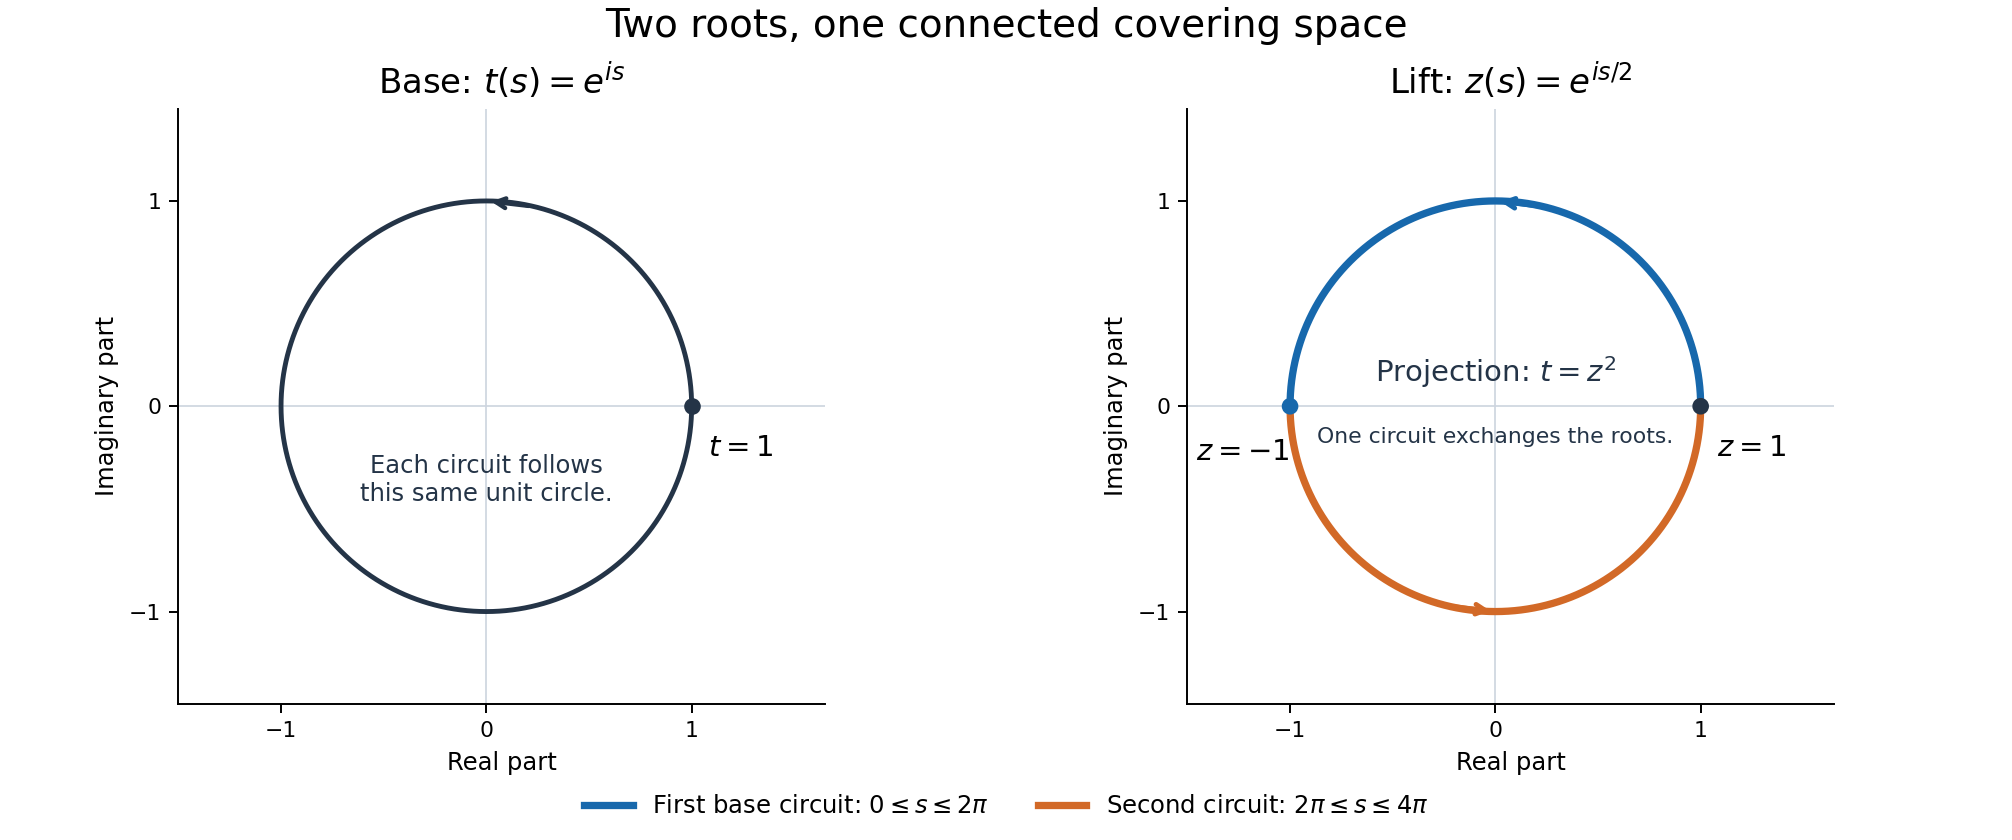
\includegraphics[keepaspectratio,alt={A double cover: one circuit in the base exchanges the roots, and two circuits close the lifted path.}]{../verification/lesson22/algebraic-cover-connectedness.png}}
\par\smallskip
\begin{flushleft}\small
\emph{Figure 22.3. Both panels are unit circles with their actual
complex coordinates. In the base the two circuits trace the same circle.
On the covering circle the first circuit traces the blue upper
semicircle from \(1\) to \(-1\), and the second traces the orange lower
semicircle back to \(1\). The projection is exactly \(z\mapsto z^2\); no
branch cut separates the total space.}
\end{flushleft}
\end{minipage}\par\medskip


The equivariant compactification in Theorem 22.39 can be compared with
Serre's freely accessible
\href{https://numdam.org/item/AST_1979__69-70__191_0.pdf}{\emph{Quelques
propriétés des groupes algébriques commutatifs}, Section 1}. For a free
exposition of the structural theorem, see Milne's
\href{https://arxiv.org/abs/1311.6060}{\emph{A Proof of the
Barsotti--Chevalley Theorem on Algebraic Groups}}. The programme proof
and its exact hypotheses used here are specified in Theorem 22.45.

\subsection{Heights of division points and translated
derivatives}\label{heights-of-division-points-and-translated-derivatives}

Fix a connected commutative algebraic group \(G/\overline{\mathbf Q}\).
All algebraic data in a finite construction descend to a number field:
choose a field containing their finitely many coefficients and the
finitely many coefficients in the identities between them. We may
therefore enlarge a fixed number field \(K\) to include the
compactification of Theorem 22.45, its split affine kernel, the
embeddings and the vector fields that we use. Constants below may depend
on these fixed choices. They never depend on the field of definition of
a variable point.

\subsubsection{Lemma 22.47. Projective height and the product
formula}\label{lemma-22.47.-projective-height-and-the-product-formula}

For a nonzero tuple \(x=(x_0,\ldots,x_N)\) in a number field \(E\) of
degree \(d_E\), put \[
 h([x])=\frac1{d_E}\left(
 \sum_{\sigma:E\hookrightarrow\mathbf C}\log\max_i|\sigma x_i|
 -\sum_{\mathfrak p}\min_i v_{\mathfrak p}(x_i)\log N\mathfrak p
 \right).
 \tag{22.110}
\] Here \(v_{\mathfrak p}(0)=+\infty\), and the second sum runs over the
nonzero prime ideals of \(\mathcal O_E\). The valuation of a nonzero
element is its exponent in the principal fractional ideal. The
expression is finite, is independent of scaling \(x\) and of enlarging
\(E\), and is nonnegative. Write \(h(a)=h([1:a])\). For \(a\ne0\) and
any specified embedding \(\sigma:E\hookrightarrow\mathbf C\), \[
 h(a^{-1})=h(a),\qquad
 \log|\sigma a|\ge-d_Eh(a).
 \tag{22.111}
\]

\textbf{Proof.} We use the proved norm and ramification formulas in
\emph{Number fields}:
\href{../NT-ANT/algebraic-integers-and-rings-of-integers.html\#3-multiplication-as-a-linear-transformation}{Proposition
1.2 on conjugates and towers},
\href{../NT-ANT/norms-class-groups-and-modules-over-dedekind-domains.html\#counting-residue-classes}{Proposition
4.1 on ideal norms}, and
\href{../NT-ANT/decomposition-of-primes-in-extensions.html\#multiplicity-residue-degree-and-the-fundamental-identity}{Theorem
5.2 on the fundamental identity}. Together they give, for
\(a\in E^\times\), \[
 \sum_\sigma\log|\sigma a|
 =\log|N_{E/\mathbf Q}(a)|
 =\sum_{\mathfrak p}v_{\mathfrak p}(a)\log N\mathfrak p .
 \tag{22.112}
\] The middle equality with the ideal sum holds first for integral
elements and then for fractions, by multiplicativity of the ideal norm.
This is the product formula in the normalization needed here. Scaling
the tuple by \(a\) adds the two equal sides of (22.112) with opposite
signs in (22.110).

For an extension \(F/E\), every complex embedding of \(E\) extends to
\([F:E]\) embeddings of \(F\). At a prime \(\mathfrak P\) above
\(\mathfrak p\), the valuation of an element of \(E\) is multiplied by
\(e(\mathfrak P/\mathfrak p)\), and
\(\log N\mathfrak P=f(\mathfrak P/\mathfrak p)\log N\mathfrak p\). The
identity \(\sum_{\mathfrak P\mid\mathfrak p}ef=[F:E]\) therefore
multiplies both sums in the numerator by \([F:E]\). The denominator is
multiplied by the same integer. Comparison in a compositum proves
independence of arbitrary containing fields.

Normalize one nonzero coordinate to \(1\). Every infinite-place
logarithm is then nonnegative, and every minimum valuation is
nonpositive. This proves nonnegativity. Scaling \([1:a^{-1}]\) by \(a\),
and permuting coordinates, gives \(h(a^{-1})=h(a)\). Each nonnegative
term \(\log\max(1,|\sigma a^{-1}|)\) is at most \(d_Eh(a^{-1})\);
negating this bound proves (22.111). \(\square\)

We will use local maximum estimates with precisely the normalization in
(22.110). At a prime \(\mathfrak p\), write
\(\|a\|_{\mathfrak p}=(N\mathfrak p)^{-v_{\mathfrak p}(a)}\); it is
multiplicative and ultrametric. At infinity sum over all embeddings, so
both members of a complex-conjugate pair occur. If a finite tuple of
fixed coefficients has local maximum at most \(C_v\), take \(C_v\ge1\).
All but finitely many finite-place constants equal \(1\). The normalized
sum of their logarithms remains unchanged on field extension, by the
calculation just made.

\subsubsection{Lemma 22.48. Polynomial evaluation and
morphisms}\label{lemma-22.48.-polynomial-evaluation-and-morphisms}

Let \(F_0,\ldots,F_M\) be homogeneous forms of degree \(d\) in \(N+1\)
variables over \(K\), and suppose their tuple is nonzero at \(x\). There
is a constant \(C\), independent of \(x\), such that \[
 h([F_0(x):\cdots:F_M(x)])\le d\,h(x)+C.
 \tag{22.113}
\] Consequently, if \(V\subset\mathbf P^N\) is a locally closed variety
and \(\psi:V\to\mathbf P^M\) is a morphism, there are \(c,d\ge1\) such
that \(h(\psi(x))\le c+d\,h(x)\) on \(V(\overline{\mathbf Q})\). For a
morphism \(V\times V\to\mathbf P^M\), one can use a bound
\(c+d(h(x)+h(y))\).

\textbf{Proof.} At a finite place, each value has norm at most the
largest coefficient norm times \(\max_i\|x_i\|_v^d\). At an infinite
embedding, the triangle inequality gives the same estimate with an
additional factor equal to the maximum number of monomials in a form.
Sum logarithms as in (22.110). The coefficient and monomial factors have
a finite, field-independent contribution \(C\), proving (22.113).

We justify the passage to a morphism even when \(V\) is not projective.
Near a point choose a source affine chart \(X_j\ne0\) and a target
affine chart containing its image. Regular functions on a locally closed
affine variety are locally fractions in its affine coordinate ring. On a
smaller principal open, all the target coordinate functions therefore
have polynomial numerators with a common polynomial denominator that is
nonzero there. Include that denominator as the target homogeneous
coordinate. Homogenize all these polynomials to a common degree using
\(X_j\). This gives a homogeneous tuple representing \(\psi\), nonzero
throughout that open. Quasi-compactness supplies finitely many such
opens and tuples. Apply (22.113) to whichever tuple is valid at the
point and take the maximum of the finitely many constants and degrees.

On a product, carry out the same construction on pairs of affine charts
and homogenize separately in \(X\) and \(Y\). A tuple of bidegree
\((a,b)\) has height bound \(a h(x)+b h(y)+C\), by the identical local
estimate. A finite cover gives the last assertion. \(\square\)

For later use, if \(R\) is a homogeneous polynomial of degree \(d\),
\(x_j\ne0\), and \(c(R)\) denotes its coefficient tuple, the same proof,
now including the constant \(1\) among the coefficients, gives \[
 h\bigl(R(x/x_j)\bigr)
 \le d\,h(x)+h([1:c(R)])+\log\binom{N+d}{N}.
 \tag{22.114}
\] Including \(1\) is essential for a scalar value: projectively
rescaling all coefficients changes that value.

\subsubsection{Proposition 22.49. Heights of line bundles on a
projective
variety}\label{proposition-22.49.-heights-of-line-bundles-on-a-projective-variety}

Let \(X/K\) be projective. To each line bundle \(\mathcal L\) one can
associate a real function \(h_{\mathcal L}\) on
\(X(\overline{\mathbf Q})\), well-defined up to a bounded function, with
\[
\begin{split}
 h_{\mathcal L\otimes\mathcal M}&=h_{\mathcal L}+h_{\mathcal M}+O(1),\\
 h_{f^*\mathcal L}&=h_{\mathcal L}\circ f+O(1).
\end{split}
\tag{22.115}
\] The second assertion is for a fixed morphism \(f:Y\to X\) between
projective varieties. If a finite family of global sections generates
\(\mathcal L\), its evaluation map \(\phi:X\to\mathbf P^r\) gives
\(h_{\mathcal L}=h\circ\phi+O(1)\). Isomorphic line bundles have heights
differing by \(O(1)\). If \(D\) is an effective Cartier divisor, then \[
 h_{\mathcal O(D)}(x)\ge-C_D\qquad(x\notin D)
 \tag{22.116}
\] for a constant independent of \(x\) and its field of definition.

\textbf{Proof.} First suppose that two finite generating families
\(S,T\) belong to the same line bundle. Their union \(U\) defines a
morphism to projective space with closed image \(Z\), because \(X\) is
projective. On \(Z\), the coordinates belonging to \(S\) have no common
zero. The strong Nullstellensatz, proved in
\href{../AG-CA/the-nullstellensatz-and-jacobson-rings.html\#2-closed-points-detect-radical-equations}{\emph{The
Nullstellensatz and Jacobson rings}, Theorem 2.2}, applied to the affine
cone shows that for each coordinate \(U_j\) some power belongs to the
homogeneous ideal generated by the coordinates in \(S\) and \(I(Z)\).
Increasing to a common exponent \(r\) and taking homogeneous components
gives \[
 U_j^r=\sum_{i\in S}U_i A_{ij}(U)\pmod{I(Z)},
 \qquad \deg A_{ij}=r-1.
 \tag{22.117}
\] The identities may be taken over \(K\): after fixing their finite
degrees, their coefficients solve linear equations over \(K\); a
solution over an extension implies consistency and hence a solution over
\(K\).

At any place, choose \(j\) with maximum \(|U_j|\) and apply the
corresponding identity. It gives
\(\max_j|U_j|^r\le C_v\max_{i\in S}|U_i|\max_j|U_j|^{r-1}\). Cancel the
nonzero last factor. At finite places \(C_v=1\) except for finitely many
primes; at infinity incorporate the number of terms. Since \(S\) is a
subtuple, the reverse inequality \(\max_S\le\max_U\) is automatic.
Summing logarithms proves \(0\le h_U-h_S\le C\). Apply the same argument
to \(T\). Thus any two generating families define heights differing by a
bounded constant.

If \(S\) generates \(\mathcal L\) and \(T\) generates \(\mathcal M\),
the products \(s_i t_j\) generate \(\mathcal L\otimes\mathcal M\). Their
local maximum is exactly \(\max_i|s_i|\max_j|t_j|\). Their height is
therefore exactly \(h_S+h_T\). Pulling back a generating family also
gives the same projective evaluation map composed with \(f\). These
observations prove both identities for globally generated bundles.

Fix a very ample bundle \(H\) with a generating family. For every
\(\mathcal L\), choose \(r\ge0\) so that \(\mathcal L\otimes H^r\) is
globally generated; this is
\href{../AG-QC/serres-theorems-on-projective-schemes.html\#2-descending-induction-proves-serre-s-theorems}{Serre's
global-generation theorem} in its ample form. Define \[
 h_{\mathcal L}=h_{\mathcal L\otimes H^r}-r h_H.
 \tag{22.118}
\] This is independent up to a bounded function of \(r\), of the
generating families and of \(H\). Indeed, two presentations
\(\mathcal L=\mathcal A\otimes\mathcal B^{-1}=\mathcal C\otimes\mathcal D^{-1}\),
with all four bundles globally generated, give isomorphic globally
generated bundles \(\mathcal A\otimes\mathcal D\) and
\(\mathcal C\otimes\mathcal B\). The preceding comparison and product
calculation show
\(h_{\mathcal A}+h_{\mathcal D}=h_{\mathcal C}+h_{\mathcal B}+O(1)\).
This also proves additivity, invariance under isomorphism and
functoriality for arbitrary line bundles, by expressing each as such a
difference. The constants in this proof are uniform over all algebraic
points, by (22.117) and the field-independence in Lemma 22.47.

Finally let \(s_D\) be the canonical section of \(\mathcal O(D)\).
Choose \(r\) with \(\mathcal O(D)\otimes H^r\) globally generated. Among
a finite generating family include all products \(s_D t_i\), where the
\(t_i\) generate \(H^r\). Outside \(D\) this subtuple is nonzero and
represents the same projective point as \((t_i)\). Enlarging a nonzero
tuple can only increase its height, since its local maxima increase in
every place. Hence \(h_{\mathcal O(D)\otimes H^r}\ge h_{H^r}\) for these
chosen families outside \(D\). Subtract and use (22.115) to obtain
(22.116). \(\square\)

\subsubsection{Proposition 22.50. Doubling and the
boundary}\label{proposition-22.50.-doubling-and-the-boundary}

Use the compactification \(q:X\to A\) of Theorem 22.39. Let \(B_a\) be
the sum of its additive infinity divisors, and \(B_m\) the sum of its
multiplicative zero and infinity divisors. Empty sums mean the zero
divisor. Then \([2]:G\to G\) extends to a morphism \(p:X\to X\),
covering \([2]:A\to A\), and \[
 p^*B_a=B_a,\qquad p^*B_m=2B_m.
 \tag{22.119}
\] There is a symmetric very ample line bundle \(M\) on \(A\) and a
positive integer \(a\) such that
\(\mathcal L=\mathcal O(B_a+B_m)\otimes q^*M^a\) is ample on \(X\).

\textbf{Proof.} Write \(X=G\times^{L_0}F\), where
\(L_0=\mathbf G_a^a\times\mathbf G_m^b\) as in Theorem 22.39; the
exponent \(a\) in the assertion is unrelated to this dimension. On
\(F=(\mathbf P^1)^{a+b}\), use \([u:v]\mapsto[2u:v]\) on each additive
factor and \([u:v]\mapsto[u^2:v^2]\) on each multiplicative factor.
Denote their product by \(p_F\). It satisfies
\(p_F(\ell\cdot z)=[2]\ell\cdot p_F(z)\). Consequently \[
 [g,z]\longmapsto[[2]g,p_F(z)]
 \tag{22.120}
\] respects the associated-bundle relation, descends to a morphism on
\(X\), and agrees with doubling on the dense open \(G\).

On an additive factor the infinity equation \(v=0\) pulls back with
multiplicity one; on a multiplicative factor each equation \(u=0\) or
\(v=0\) pulls back with multiplicity two. These are scheme-theoretic
Cartier-divisor computations in local frames. The factors changing those
frames are units. Thus they give exactly (22.119), with no extra
component over the base.

Choose a very ample bundle \(H_A\) on \(A\). The tensor product
\(M=H_A\otimes[-1]^*H_A\) is symmetric and very ample: the product of
the two embeddings followed by the Segre embedding is an embedding with
this bundle. The identity \([2]^*M\simeq M^4\) is
\href{https://github.com/KokunoYumeto/open-math-courses-public/blob/146dc81802e69cf262fb6cc65c1b9f74e71f4625/docs/courses/AG-GS/src/abelian-varieties.md\#5-multiplication-pulls-back-quadratically}{\emph{Abelian
varieties}, Theorem 5.1}, proved there from the cube theorem.

For ampleness on \(X\), keep the line convention for \(\mathbf P(E_i)\)
used in Theorem 22.39, and let \(H_i=\mathcal O_{\mathbf P(E_i)}(1)\),
pulled back to \(X\). In an additive factor the projection
\(E_i\to\mathcal O_A\) gives the infinity divisor, whose bundle is
\(H_i\). In a multiplicative factor \(E_i=M_i\oplus\mathcal O_A\), the
two projections give the infinity and zero divisor bundles \(H_i\) and
\(H_i\otimes q^*M_i\), respectively. Hence \[
 \mathcal O(B_a+B_m)
 \simeq\left(\bigotimes_i H_i^{d_i}\right)\otimes q^*Q,
 \quad d_i=1\text{ or }2,\quad Q=\bigotimes_{\text{multiplicative }i}M_i.
 \tag{22.121}
\] As in Theorem 22.39, choose \(r\) such that all
\(E_i^\vee\otimes M^r\) are globally generated. The resulting closed
immersion into \(A\times\prod_i\mathbf P^{N_i-1}\), followed on the
projective factors by their degree-\(d_i\) Veronese maps and their Segre
map, has relative hyperplane bundle
\((\bigotimes_i H_i^{d_i})\otimes q^*M^{r\sum_i d_i}\). Choose \(a\) so
that \(Q\otimes M^{a-r\sum_i d_i}\) is very ample on \(A\). Such an
\(a\) exists: Serre gives global generation after a sufficiently high
twist, and tensoring a globally generated line bundle with a very ample
bundle is very ample, by the product-map and Segre argument. Embedding
the base by this bundle and taking the final Segre map proves ampleness,
in fact very ampleness, of \(\mathcal L\). If there are no affine
factors, simply take \(\mathcal L=M^a\) on \(A\). \(\square\)

\subsubsection{Theorem 22.51. Heights along repeated division by
two}\label{theorem-22.51.-heights-along-repeated-division-by-two}

Fix a projective embedding \(\iota:G\hookrightarrow\mathbf P^N\) and
\(\gamma\in G(\overline{\mathbf Q})\). There is a constant
\(C_\gamma\ge1\) such that for every integer \(e\ge0\) and every point
\(\eta\) with \([2^e]\eta=\gamma\), \[
 h(\iota(\eta))\le C_\gamma(1+e).
 \tag{22.122}
\] The bound holds for every division point, regardless of its degree.

\textbf{Proof.} First construct the one scaling property of a canonical
height that is needed. For the symmetric very ample \(M\) of Proposition
22.50, choose its embedding height \(h_M\ge0\). By (22.115) and
\([2]^*M\simeq M^4\), there is a fixed \(C_0\) with
\(\left|h_M([2]z)-4h_M(z)\right|\le C_0\). Successive terms of
\(4^{-r}h_M([2^r]z)\) differ by at most \(C_0\,4^{-r-1}\), uniformly in
\(z\). The geometric series proves convergence and gives \[
 \widehat h_M(z)=\lim_{r\to\infty}4^{-r}h_M([2^r]z)\ge0,\quad
 |\widehat h_M-h_M|\le C_0/3,\quad
 \widehat h_M([2]z)=4\widehat h_M(z).
 \tag{22.123}
\] No quadratic pairing or positivity theorem for nontorsion points is
needed for these assertions.

Use a projective embedding of \(X\) given by a sufficiently large power
of the ample bundle \(\mathcal L\) in Proposition 22.50; divide its
height by that power and denote the resulting nonnegative height by
\(h_{\mathcal L}\). Equations (22.115), (22.119) and (22.123) give,
uniformly on \(G\), \[
 h_{\mathcal L}([2]x)-h_{\mathcal L}(x)
 =h_{\mathcal O(B_m)}(x)+3a\,\widehat h_M(qx)+O(1)\ge-C_1.
 \tag{22.124}
\] Indeed \(B_m\) is effective and disjoint from \(G\), so (22.116)
bounds its height below. The remaining displayed term is nonnegative.

All points \(\eta,[2]\eta,\ldots,[2^e]\eta\) lie in \(G\). Iterating
(22.124) gives \(h_{\mathcal L}(\eta)\le h_{\mathcal L}(\gamma)+eC_1\).
Finally compare the morphism \(\iota\) with the embedding induced by a
power of \(\mathcal L\), using Lemma 22.48 on the locally closed \(G\).
Absorb its fixed degree and constant into \(C_\gamma\), obtaining
(22.122). \(\square\)

\subsubsection{Corollary 22.52. Heights of multiples with a uniform
polynomial
exponent}\label{corollary-22.52.-heights-of-multiples-with-a-uniform-polynomial-exponent}

For a fixed projective embedding of \(G\), there are constants \(C\ge1\)
and an integer \(\kappa\ge1\) such that \[
 h([s]x)+1\le C(s+1)^\kappa\bigl(h(x)+1\bigr)
 \qquad(s\ge0,\ x\in G(\overline{\mathbf Q})).
 \tag{22.125}
\] In particular, put \(b=2^e\), let \([b]\eta=\gamma\), and suppose
\(1\le b\le S\) and \(0\le s\le bS\). For a fixed integer \(B\) and a
fixed constant \(C_\gamma'\), \[
 h([s]\eta)\le C_\gamma'S^B.
 \tag{22.126}
\] One may take \(B=2\kappa+1\), increasing \(C_\gamma'\) as needed.

\textbf{Proof.} Lemma 22.48 applied to addition gives
\(h(x+y)+1\le A(h(x)+h(y)+2)\) for some \(A\ge1\). Set
\(M_r=\max_{0\le s\le2^r}(h([s]x)+1)\). Every integer \(s\le2^{r+1}\) is
a sum of two nonnegative integers at most \(2^r\), so
\(M_{r+1}\le2A M_r\). Also \(M_0\le C_2(h(x)+1)\), because \(h(0)\) is
fixed. Choose an integer \(\kappa\) with \(2^\kappa\ge2A\). For
\(s\ge1\), take \(r=\lceil\log_2 s\rceil\), so \(2^r\le2s\); iteration
proves (22.125). Increasing \(C\) covers \(s=0\).

By Theorem 22.51, \(h(\eta)+1\le C_\gamma(1+e)\). Since \(b\le S\),
\(1+e\le C_3 S\) for \(S\ge1\), and \(s+1\le S^2+1\le2S^2\). Insert
these in (22.125) to obtain (22.126). \(\square\)

\subsubsection{Lemma 22.53. Distinct points obtained by dyadic
division}\label{lemma-22.53.-distinct-points-obtained-by-dyadic-division}

Let \(u\ne0\) in \(\operatorname{Lie}G(\mathbf C)\), let
\(\gamma=\exp_G(u)\) be algebraic, and put \(\eta_e=\exp_G(u/2^e)\).
There is an integer \(c\ge1\), depending on \(u\) but not on \(e,S\),
such that for every sufficiently large \(e\) and every integer
\(S\ge1\), \[
 \#\{[s]\eta_e:0\le s\le2^e S\}
 \ge\frac{2^e}{2c}\,\#\{[s]\gamma:0\le s\le S\}.
 \tag{22.127}
\] Moreover, if \(G,\gamma\) are defined over \(K\) and \(n=\dim G\),
all these points lie in one number field \(K(\eta_e)\) with
\([K(\eta_e):\mathbf Q]\le[K:\mathbf Q]\,2^{2ne}\).

\textbf{Proof.} Algebraicity and the degree bound are Theorem 22.43,
applied to \([2^e]\eta_e=\gamma\); the group law puts every multiple in
the same field. If \(\gamma\) is nontorsion, so is \(\eta_e\). The two
cardinalities are \(2^eS+1\) and \(S+1\), respectively. Their ratio is
at least \(2^e/2\), so take \(c=1\).

Suppose instead that \(\gamma\) has exact order \(M\). The vector
\(v=Mu\) is a nonzero element of the period lattice
\(\Lambda=\ker\exp_G\), which is a free abelian group of finite rank by
Proposition 22.35. Write \(v=\sum_i a_i\lambda_i\) in a lattice basis,
and let \(g=\gcd_i|a_i|>0\). Exactness of the order \(M\) implies
\(\gcd(g,M)=1\): a common prime divisor would make \((M/p)u=v/p\) a
period.

The order of \(\eta_e\) is the least positive \(t\) for which every
\(ta_i/(M2^e)\) is an integer. Bézout's identity for the integers
\(a_i\) therefore gives the exact order \[
 \operatorname{ord}(\eta_e)
 =\frac{M2^e}{\gcd(g,M2^e)}
 =\frac{M2^e}{2^\nu}
 \quad(e\ge\nu),\qquad \nu=v_2(g).
 \tag{22.128}
\] Put \(c=2^\nu\). The initial number of distinct multiples is
\(q=\min(S+1,M)\), and the divided number is \(\min(2^eS+1,M2^e/c)\).
Since \(S\ge(S+1)/2\ge q/2\) and \(M\ge q\), both entries in this
minimum are at least \(2^e q/(2c)\). This proves (22.127), including
\(M=1\), the case of a nonzero period \(u\). \(\square\)

\subsubsection{Proposition 22.54. The height cost of a translated
derivative}\label{proposition-22.54.-the-height-cost-of-a-translated-derivative}

Choose finitely many bihomogeneous tuples \(E_\alpha(X,Y)\) representing
the addition map on open subsets covering \(G\times G\), as in Lemma
22.48. Fix an affine neighborhood of the identity with algebraic
coordinates \(y=(y_1,\ldots,y_r)\), realized as a closed affine variety,
and polynomial lifts of fixed invariant derivations there as in Lemma
22.11. If an extra principal localization is necessary, include its
inverse as an additional coordinate. In these coordinates the projective
coordinates \(Y(y)\) on a chart containing the identity are polynomials;
one homogeneous coordinate is \(1\).

Let \(P\in\mathbf Z[Z_0,\ldots,Z_N]\) be homogeneous of degree
\(D\ge1\), with coefficients of absolute value at most \(H\ge1\). For a
derivative word \(I\) of length \(t\), define \[
 J_{\alpha,I}(X)=
 \left.D_I\bigl(P(E_\alpha(X,Y(y)))\bigr)\right|_{y=y(0)}.
 \tag{22.129}
\] There are constants \(a,C\ge1\), independent of \(P,D,H,t\), such
that each \(J_{\alpha,I}\) is homogeneous of degree \(a_\alpha D\le aD\)
in \(X\), has coefficients in \(K\), and satisfies \[
 h([1:c(J_{\alpha,I})])
 \le \log H+C(D+t)\log(D+t+2).
 \tag{22.130}
\] Zero polynomials are permitted, with coefficient height zero. For
\(x\in G(E)\), normalize a nonzero homogeneous coordinate \(x_j\) to
\(1\). If \(J_{\alpha,I}(x/x_j)\ne0\), then \[
 \log\left|\sigma J_{\alpha,I}(x/x_j)\right|
 \ge-[E:\mathbf Q]\!
 \left(\log H+C(D+t)\log(D+t+2)+aD\,h(x)\right).
 \tag{22.131}
\] Here \(E\) contains \(K\), and \(C\) has been enlarged to include the
monomial count. The point-height term is multiplied by \(D\), not by
\(t\).

\textbf{Proof.} Let the bidegree of \(E_\alpha\) be
\((a_\alpha,b_\alpha)\). Before differentiation, substitution into \(P\)
gives degree exactly \(a_\alpha D\) in \(X\), unless the polynomial is
zero, and degree at most \(c_0D\) in \(y\), for a fixed \(c_0\). The
derivations act only on \(y\), so homogeneity and degree in \(X\) are
preserved.

The fixed addition and coordinate polynomials have a fixed common
integer denominator and bounded coefficient norms at every embedding of
\(K\). Expanding \(P\) shows that its substituted polynomial has common
denominator at most \(q_0^D\) and coefficient norm at most
\(H(D+1)^N A_0^D\), after increasing fixed \(q_0,A_0\ge1\). Propositions
22.12--22.13, with \(D_Y=c_0D\) and the fixed algebraic evaluation point
\(y(0)\), consequently give a positive integer \(Q_{D,t}\) and a real
\(R_{D,t}\ge1\) such that \[
\begin{split}
 Q_{D,t}J_{\alpha,I}&\in\mathcal O_K[X],\\
 \log Q_{D,t}&\le C_4(D+t),\\
 \max_\sigma\|J_{\alpha,I}^\sigma\|_1&\le R_{D,t},\\
 \log R_{D,t}&\le\log H+C_5(D+t)\log(D+t+2).
\end{split}
\tag{22.132}
\] At a finite prime the coefficient tuple \([1:c(J)]\) has local
maximum at most that of \(1/Q_{D,t}\) if this exceeds \(1\); its total
normalized finite contribution is at most \(\log Q_{D,t}\), by (22.112)
for this rational integer. Its infinite contribution is at most
\(\log R_{D,t}\). This proves (22.130).

Apply (22.114) to the normalized tuple \(x/x_j\), then (22.111) to the
nonzero resulting algebraic number. Since
\(\log\binom{N+aD}{N}\le C_6D\log(D+2)\), it is absorbed in (22.130).
This proves (22.131). In particular, evaluating a derivative at a moving
point directly is unnecessary: differentiating the second argument of
the addition law at the fixed identity keeps the moving-point degree
bounded by \(aD\). \(\square\)

\subsubsection{Corollary 22.55. Extrapolation with any fixed polynomial
growth
exponent}\label{corollary-22.55.-extrapolation-with-any-fixed-polynomial-growth-exponent}

Fix \(n\ge2\), \(m\ge1\), positive constants \(C_a,C_b\), and real
numbers \(B,\rho\ge1\). Choose an integer \(k\ge\max(5,B,2\rho)\), and
put \(K=nk+2+12nm\), \(C_0=2K+1\). Choose \(b=2^e>16C_0(C_a+C_b)\), let
\(S=b^{2n+1}\), and use the parameters \(A,D,T,M,V\) of (22.50), with
any \(1\le q\le S+1\). Suppose \(f\) is entire and vanishes to order at
least \(M\) at \(0,\ldots,S\). Suppose also that \[
\begin{split}
 \log\max_{|z|\le S^2}|f(z)|
 &\le C_a\{V+D(S^B+S^{2\rho})\},\\
 f(s/b)\ne0\quad&\Longrightarrow\quad
 \log|f(s/b)|\ge-C_b b^{2n}\{V+DS^B\}
 \quad(0\le s\le bS).
\end{split}
\tag{22.133}
\] Then \(f(s/b)=0\) for all these integers \(s\).

\textbf{Proof.} The zero function causes no difficulty. As in
Proposition 22.21, \(V\le2KA\log S\), \(M\ge A/8\), and \(D=A/S^k\). The
new restrictions on \(k\) give \(DS^B\le A\) and \(DS^{2\rho}\le A\).
Since \(\log S\ge2\), each expression in braces in (22.133) is at most
\(C_0A\log S\). Lemma 22.19 bounds the logarithm at a nonzero \(f(s/b)\)
above by \(A\log S(C_a C_0-S/16)\). Combining this with its lower bound
yields \(S\le16C_0(C_a+C_b b^{2n})\), contrary to \(S=b^{2n+1}\) and the
chosen lower bound on \(b\). This is the same integer comparison as in
(22.53), with the larger fixed exponents absorbed by \(k\). \(\square\)

Thus the extrapolation argument can use any \emph{proved finite} growth
order \(\rho\). A claimed order, without a construction and its
estimates, does not supply the first line of (22.133).

\subsubsection{Lemma 22.56. Clearing point denominators without a
derivative-order
penalty}\label{lemma-22.56.-clearing-point-denominators-without-a-derivative-order-penalty}

Let \(x=[x_0:\cdots:x_N]\in\mathbf P^N(K)\), choose \(x_j\ne0\), and
write \(z_i=x_i/x_j\). There is a positive rational integer \(b_x\) such
that \[
 b_xz_i\in\mathcal O_K,\qquad
 \log b_x\le m h(x),\qquad
 \max_{\sigma,i}\log\max(1,|\sigma z_i|)\le m h(x),
 \quad m=[K:\mathbf Q].
 \tag{22.134}
\] For the coefficient functions \(J_{\alpha,I}\) obtained by applying
(22.129) to a single degree-\(D\) monomial \(P\), their values at \(z\)
can consequently be expanded in a fixed integral basis of
\(\mathcal O_K\) after multiplication by a positive integer. The
resulting integer coefficients have absolute value at most \[
 \exp\!\left(C\{(D+t)\log(D+t+2)+D h(x)\}\right),
 \tag{22.135}
\] where \(C\) depends only on the fixed data and \(K\). The same
denominator works for all monomials and derivative words of order at
most \(t\) at this point. Different points may use different
denominators.

\textbf{Proof.} Put
\(r_{\mathfrak p}=\max(0,-\min_i v_{\mathfrak p}(z_i))\) and
\(\mathfrak d=\prod_{\mathfrak p}\mathfrak p^{r_{\mathfrak p}}\).
Because \(z_j=1\), the finite part of \(m h(x)\) is exactly
\(\log N\mathfrak d\); the infinite part is nonnegative. Set
\(b_x=N\mathfrak d\). The finite abelian group
\(\mathcal O_K/\mathfrak d\) has this order, so multiplication by
\(b_x\) kills it, proving \(b_x\mathcal O_K\subset\mathfrak d\). It
follows that
\(v_{\mathfrak p}(b_xz_i)\ge r_{\mathfrak p}+v_{\mathfrak p}(z_i)\ge0\)
at every prime. This proves integrality and the bound for \(b_x\). Each
nonnegative infinite summand in (22.110) is individually at most
\(m h(x)\), proving the last bound in (22.134).

For a monomial \(P\), (22.132) holds with \(H=1\). Choose its
denominator uniformly in the monomial, the chart index and all words of
length at most \(t\), using the fixed denominators in the proof of
Propositions 22.12--22.13; a fixed integer raised to \(C_1(D+t)\)
suffices. Multiply further by \(b_x^{aD}\). Every evaluated coefficient
is now integral, since its degree in \(z\) is at most \(aD\). At any
embedding, its absolute value is bounded by \[
 Q_{D,t}\,b_x^{aD}R_{D,t}
       \bigl(\max_i\max(1,|\sigma z_i|)\bigr)^{aD}.
 \tag{22.136}
\] Taking logarithms and using (22.132)--(22.134) gives (22.135),
initially for conjugate absolute values.

To pass to integer coordinates, let \(\omega_1,\ldots,\omega_m\) be an
integral basis. The matrix \((\sigma_i\omega_j)_{i,j}\) is nonsingular:
its determinant squared is the nonzero field discriminant, as proved in
\href{../NT-ANT/discriminants-and-integral-bases.html\#a-determinant-that-measures-a-basis}{\emph{Discriminants
and integral bases}, Proposition 2.1}. Its fixed inverse bounds each
coordinate of an algebraic integer by a fixed multiple of the maximum
absolute value of its conjugates. Absorb this factor in \(C\). This
proves the integer coefficient bound. Multiplying one linear equation by
its own nonzero denominator preserves its solution set; there is no need
to multiply together denominators from distinct points. \(\square\)

\subsubsection{Example 22.57. Additive and multiplicative division have
different
heights}\label{example-22.57.-additive-and-multiplicative-division-have-different-heights}

Embed \(\mathbf G_a\) in \(\mathbf P^1\) by \(x\mapsto[1:x]\), and
divide the point \(1\) by \(2^e\). In the primitive integer coordinates
\([2^e:1]\), formula (22.110) gives \[
 h([1:2^{-e}])=e\log2.
 \tag{22.137}
\] Thus a bound uniform in \(e\), independent of the division point,
would already fail for the additive group.

For \(\mathbf G_m\), divide \(2\) by \(2^e\) and choose any root
\(\alpha_e\) of \(X^{2^e}-2\). Height satisfies \(h(a^r)=r h(a)\) for
\(r\ge1\): in the normalized tuple \([1:a]\), both every infinite
maximum and every negative valuation are multiplied by \(r\). Hence \[
 h([1:\alpha_e])=2^{-e}\log2.
 \tag{22.138}
\] All choices of the root obey this identity. The positive real root is
only one representative for drawing it. In the Segre embedding of
\(\mathbf G_a\times\mathbf G_m\), local maxima multiply, so the height
of \((2^{-e},\alpha_e)\) is exactly \((e+2^{-e})\log2\). These formulas
illustrate both the growth allowed by Theorem 22.51 and the distinction
between a small complex absolute value and a small arithmetic height.

\begin{minipage}[t]{\linewidth}
\centering
\pandocbounded{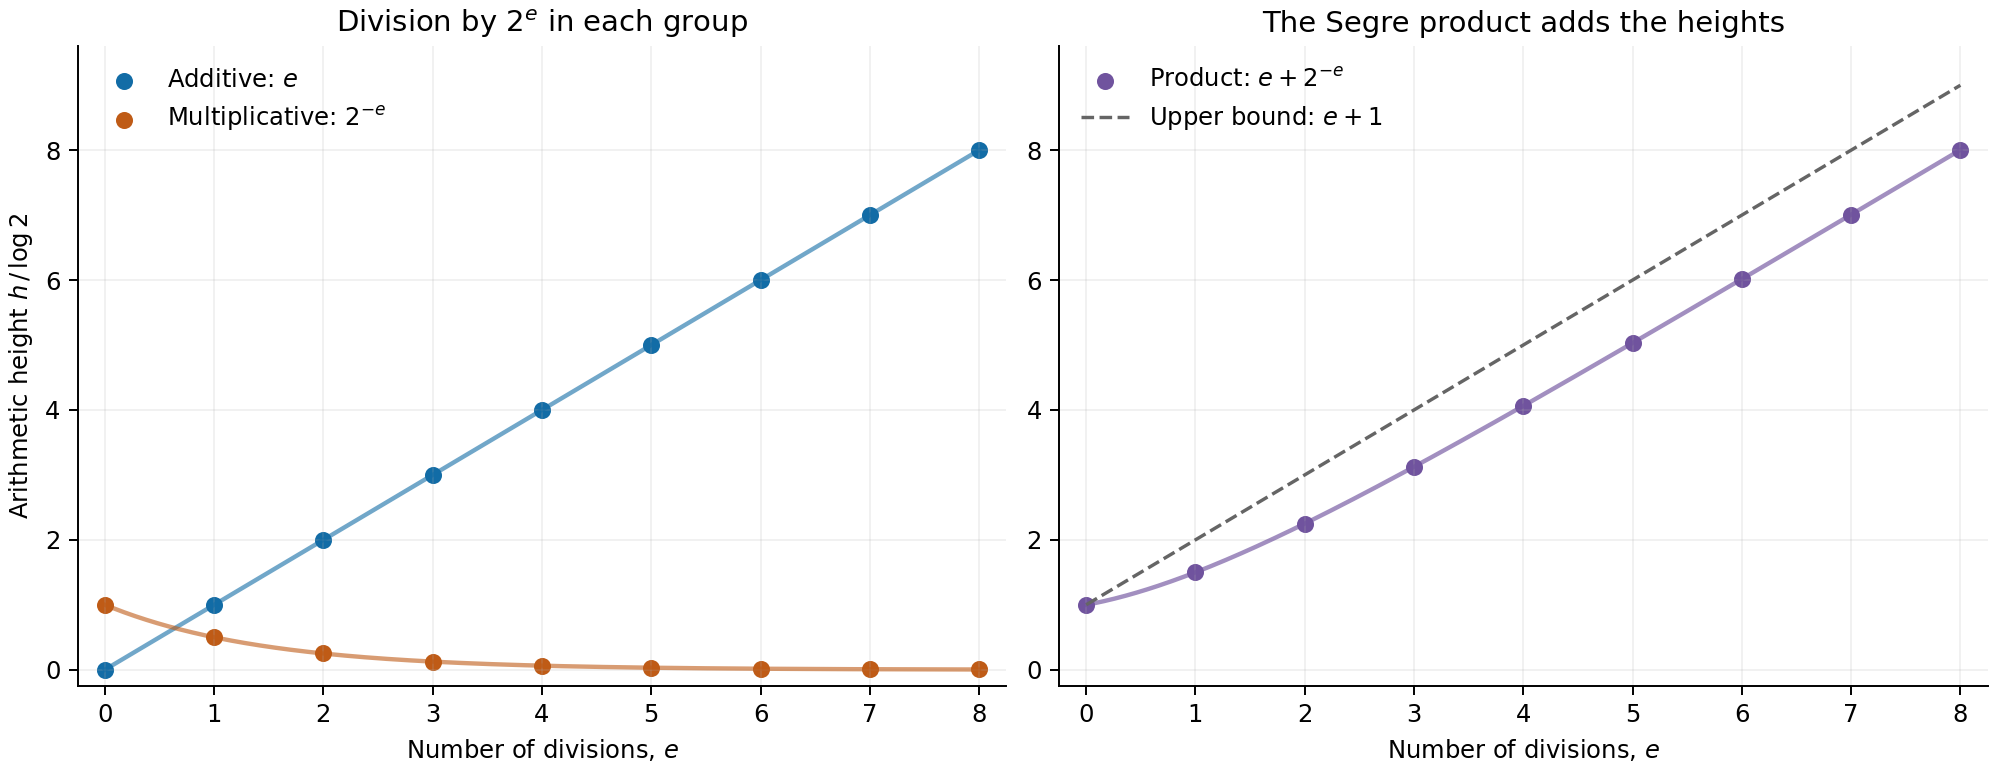
\includegraphics[keepaspectratio,alt={Exact heights under repeated division by two in the additive and multiplicative groups, and in their Segre product.}]{../verification/lesson22/dyadic-division-heights.png}}
\par\smallskip
\begin{flushleft}\small
\emph{Figure 22.4. Dots are the actual division points' heights, divided
by \(\log2\), at integer \(e\). The connecting curves interpolate the
explicit formulas \(e\), \(2^{-e}\), and \(e+2^{-e}\). They do not
assert that the groups have a division operation indexed by
nonintegers.}
\end{flushleft}
\end{minipage}\par\medskip


Theorem 22.51 and Corollary 22.52 give the point heights for (22.131),
while Lemma 22.53 controls the field degree and the number of distinct
divided points. Lemma 22.56 supplies the integer row bounds used to
construct the auxiliary polynomial. To turn them into an analytic
subgroup theorem one must also prove the analytic growth and
normalization estimates and propagate all the required jets; the height
inequalities alone do not assert that conclusion.

For comparison with the classical geometric height construction, see
Serre's freely accessible
\href{https://numdam.org/item/AST_1979__69-70__191_0.pdf}{\emph{Quelques
propriétés des groupes algébriques commutatifs}, Sections 1--2}. The
projective-height and line-bundle arguments needed above have been
proved here from the specified programme results.

\subsection{An entire lift with controlled
normalization}\label{an-entire-lift-with-controlled-normalization}

An algebraic value estimate applies to normalized projective
coordinates. An analytic zero estimate applies to an entire function.
Passing between them introduces a scalar, and an upper bound for that
scalar does not give the lower bound required by Liouville's inequality.
We construct a homogeneous entire lift whose norm is bounded in both
directions. A finite growth order suffices, by Corollary 22.55.

\subsubsection{\texorpdfstring{Lemma 22.58. A polynomially bounded
solution of a closed \(\bar\partial\)
equation}{Lemma 22.58. A polynomially bounded solution of a closed \textbackslash bar\textbackslash partial equation}}\label{lemma-22.58.-a-polynomially-bounded-solution-of-a-closed-barpartial-equation}

Let \(a=\sum_{j=1}^n a_j\,d\bar z_j\) be a smooth \((0,1)\)-form on
\(\mathbf C^n\), with \(\bar\partial a=0\). Suppose \(n\ge1\), \(s\ge0\)
is an integer, and the coefficients and their first real derivatives
satisfy \[
 |a(z)|+|Da(z)|\le C(1+|z|)^s.
 \tag{22.139}
\] There is a smooth function \(g\) with \[
 \bar\partial g=a,\qquad |g(z)|\le C'(1+|z|)^{n+s+3}.
 \tag{22.140}
\]

\textbf{Proof.} We derive the weighted estimate and its domain extension
directly. Orthogonal projection and the Riesz representation theorem are
proved in
\href{../foundations-of-von-neumann-algebras/hilbert-spaces-and-compact-operators.html}{\emph{Hilbert
spaces and compact operators}}.

Set \(N=n+s+3\), \(\varphi=N\log(1+|z|^2)\), and
\(\lambda=N/(1+|z|^2)^2\). Direct differentiation gives \[
 \varphi_{j\bar k}
 =N\frac{(1+|z|^2)\delta_{jk}-\bar z_j z_k}{(1+|z|^2)^2},
 \qquad
 \sum_{j,k}\varphi_{j\bar k}v_j\bar v_k\ge\lambda|v|^2.
 \tag{22.141}
\] The last inequality is Cauchy--Schwarz. Use the same weight
\(e^{-\varphi}\) on functions, \((0,1)\)-forms and \((0,2)\)-forms. Let
\(T=\bar\partial\) on functions and \(S=\bar\partial\) on
\((0,1)\)-forms, with their distributional maximal domains; when \(n=1\)
the last space is zero.

For a smooth compactly supported form \(v=\sum_jv_j\,d\bar z_j\), put
\(A_j=\partial/\partial\bar z_j\). Integration by parts against the
weight gives \(A_j^*=-\partial/\partial z_j+\varphi_j\), so
\(T^*v=\sum_j A_j^*v_j\). The coefficients of \(Sv\) are
\(A_jv_k-A_kv_j\), for \(j<k\). Expanding their squared norms gives the
sum of \(\|A_kv_j\|_\varphi^2\) minus
\(\sum_{j,k}\langle A_kv_j,A_jv_k\rangle_\varphi\). In the expansion of
\(\|T^*v\|_\varphi^2\), move \(A_k^*\) from the second factor to the
first. The identity \[
 A_kA_j^*=A_j^*A_k+\varphi_{j\bar k}
\] then cancels exactly those cross terms. Thus \[
 \|T^*v\|_\varphi^2+\|Sv\|_\varphi^2
 =\sum_{j,k}\|A_kv_j\|_\varphi^2
  +\int\sum_{j,k}\varphi_{j\bar k}v_j\bar v_k e^{-\varphi}.
\] Dropping the first, nonnegative sum and using (22.141) yields \[
 \int\lambda|v|^2e^{-\varphi}
 \le\|T^*v\|_\varphi^2+\|Sv\|_\varphi^2.
 \tag{22.142}
\] It extends to \(\operatorname{Dom}T^*\cap\operatorname{Dom}S\). First
multiply by \(\chi(z/R)\), where \(\chi\) is smooth, compactly
supported, and one near the origin. The commutators with \(S\) and the
weighted adjoint of \(T\) are multiplication by first derivatives of the
cutoff, bounded by \(C/R\); their weighted norms tend to zero. Testing
against \(\operatorname{Dom}T\) proves the cutoff identity for the
Hilbert-space adjoint itself. Thus these cutoffs converge in the joint
graph norm.

For a compactly supported form, convolve each coefficient with a smooth
probability mollifier \(\rho_\epsilon\) supported in a
radius-\(\epsilon\) ball. All weights on a fixed compact neighbourhood
of the support are bounded above and below. The constant-coefficient
operator \(S\) commutes with convolution. So does the principal part
\(-\sum_j\partial v_j/\partial z_j\) of \(T^*\), which belongs to
\(L^2\) there because \(T^*v\) and \(\sum_j\varphi_jv_j\) do. For its
multiplication term, the difference \[
 \varphi_j(x)(v_j*\rho_\epsilon)(x)
       -(\varphi_jv_j)*\rho_\epsilon(x)
 =\int[\varphi_j(x)-\varphi_j(x-y)]v_j(x-y)\rho_\epsilon(y)\,dy
\] has \(L^2\)-norm at most \(\omega_j(\epsilon)\|v_j\|_2\), where
\(\omega_j\) is the modulus of continuity of \(\varphi_j\) on that
compact neighbourhood. This bound follows by integrating the
translation-invariant \(L^2\)-norm against \(\rho_\epsilon\), and tends
to zero. Convolution approximates each remaining \(L^2\) term, proving
convergence in the joint graph norm. Finally \(\lambda\) is bounded, so
the left side of (22.142) converges as well.

The quantity \[
 A=\int_{\mathbf C^n}\frac{|a|^2}{\lambda}e^{-\varphi}\,dV
 \tag{22.143}
\] is finite. At large radius its radial majorant is a constant times
\(r^{2s+4-2N+2n-1}=r^{-3}\). In particular \(a\in L^2(\varphi)\) and
\(a\in\ker S\).

The subspace \(\ker S\) is closed: convergence in the weighted space
implies local \(L^2\) convergence and hence convergence as
distributions, so a limit of forms with zero distributional
\(\bar\partial\) still has zero \(\bar\partial\). For
\(v\in\operatorname{Dom}T^*\), decompose \(v=v_0+v_\perp\) by orthogonal
projection onto \(\ker S\). Since \(\operatorname{Im}T\subset\ker S\),
\(v_\perp\) belongs to \(\operatorname{Dom}T^*\) and \(T^*v_\perp=0\).
Thus \(v_0\in\operatorname{Dom}T^*\cap\ker S\). Weighted Cauchy--Schwarz
and (22.142) show \[
 |\langle a,v\rangle_\varphi|
 =|\langle a,v_0\rangle_\varphi|
 \le A^{1/2}\left(\int\lambda|v_0|^2e^{-\varphi}\right)^{1/2}
 \le A^{1/2}\|T^*v\|_\varphi .
 \tag{22.144}
\] Consequently the functional on \(\operatorname{Im}T^*\) defined by
the left pairing is well-defined and bounded. Extend it continuously to
its closure and by zero on the orthogonal complement. The Hilbert-space
Riesz representation theorem gives \(g\in L^2(\varphi)\) with norm at
most \(A^{1/2}\) and \(Tg=a\) in distributions.

Here are the local regularity and pointwise estimates. In real dimension
\(d=2n\), the equation implies
\(\Delta g=4\sum_j\partial a_j/\partial z_j=:F\). On a ball of radius
two about \(z_0\), \(F\) is smooth and bounded by \(C_1(1+|z_0|)^s\).
Choose a smooth cutoff equal to one on the ball of radius \(3/2\),
supported in that radius-two ball. The Laplace fundamental solution is
\[
 \Gamma_d(x)=
 \begin{cases}
 (2\pi)^{-1}\log|x|,&d=2,\\
 ((2-d)|\mathbf S^{d-1}|)^{-1}|x|^{2-d},&d>2.
 \end{cases}
 \tag{22.145}
\] It is harmonic off zero, locally integrable, and its outward flux
through any centered sphere is one. Integration by parts on the
complement of a radius-\(\epsilon\) ball and then letting
\(\epsilon\downarrow0\) proves \(\Delta\Gamma_d=\delta_0\). Convolve it
with the cut-off \(F\). This gives a smooth function \(v\) with
\(\Delta v=F\) on the radius-\(3/2\) ball and
\(\sup_{|z-z_0|\le1}|v(z)|\le C_2(1+|z_0|)^s\). Smoothness follows by
moving derivatives to the smooth compactly supported factor; the
supremum bound follows from local integrability of \(\Gamma_d\) on a
ball of fixed radius.

The distribution \(g-v\) is harmonic there and therefore has a smooth
harmonic representative. For completeness, mollify it on a smaller ball.
The mollifications are smooth and harmonic. The spherical-mean identity
for a smooth harmonic function follows by differentiating its spherical
average and applying the divergence theorem to its zero Laplacian. Hence
convolution with any fixed smooth radial probability kernel of
sufficiently small support leaves each mollification unchanged on a
still smaller ball. Pass to distributions to see that the original
distribution equals its convolution with that fixed smooth kernel. It is
therefore smooth and harmonic. This also proves the local assertion
without an unproved regularity assumption.

The mean-value identity and Cauchy--Schwarz now bound
\(|g(z_0)-v(z_0)|\) by a fixed constant times
\(\|g-v\|_{L^2(B(z_0,1))}\). The global weighted bound gives \[
 \|g\|_{L^2(B(z_0,1))}
 \le C_3(1+|z_0|)^N\|g\|_\varphi.
 \tag{22.146}
\] Combine this with the bound for \(v\). As \(N>s\), the result is
(22.140). The local smooth representatives agree as distributions on
overlaps, so \(g\) is globally smooth. \(\square\)

\subsubsection{Theorem 22.59. A homogeneous entire lift with two-sided
finite-order
bounds}\label{theorem-22.59.-a-homogeneous-entire-lift-with-two-sided-finite-order-bounds}

Let \(G/\mathbf C\) be a connected commutative algebraic group of
dimension \(n\ge1\), and let \(G\subset X\hookrightarrow\mathbf P^N\) be
the smooth projective equivariant compactification of Theorem 22.45 with
a fixed projective embedding. Identify
\(\operatorname{Lie}G(\mathbf C)\) with \(\mathbf C^n\). There is an
entire map \(\Phi:\mathbf C^n\to\mathbf C^{N+1}\setminus\{0\}\)
representing the composite exponential map into \(\mathbf P^N\), and a
constant \(C\), such that \[
 e^{-C(1+|z|)^\rho}\le
 \left(\sum_{j=0}^N|\Phi_j(z)|^2\right)^{1/2}
 \le e^{C(1+|z|)^\rho},
 \qquad \rho=n+4.
 \tag{22.147}
\]

\textbf{Proof.} On the line bundle \(L=\mathcal O_X(1)\), use the metric
induced by the projective embedding: if \(s_0,\ldots,s_N\) are the
coordinate sections, then \(\sum_j|s_j(x)|_L^2=1\). Explicitly, in a
holomorphic frame with \(s_j=f_j e\), set
\(|e|_L^2=(\sum_j|f_j|^2)^{-1}\). The coordinate sections have no common
zero, so this defines a smooth positive Hermitian metric on all of
\(X\).

We recall and check the connection formulas we need. In a holomorphic
line-bundle frame with metric \(h=|e|^2\), put
\(\nabla e=(\partial\log h)e\). Under \(e'=f e\) with \(f\) holomorphic
and nowhere zero, \(\partial\log h'=\partial\log h+f^{-1}df\), exactly
the transformation law for a connection. Its \((0,1)\) part is the
holomorphic \(\bar\partial\) operator. The identity
\(d h=h(\partial\log h+\overline{\partial\log h})\) proves metric
compatibility. Its curvature is
\(d\partial\log h=\bar\partial\partial\log h\), a smooth closed form of
type \((1,1)\).

Pull this connection and metric back by
\(\exp_G:\mathbf C^n\to G\subset X\). Its curvature coefficients and
their first real derivatives are bounded uniformly on \(\mathbf C^n\).
Indeed, the differential of \(\exp_G\) sends each constant real
coordinate vector to the corresponding real or imaginary part of an
invariant holomorphic vector field. Theorem 22.39 extends these fields
smoothly to the compact \(X\). A curvature coefficient is therefore the
pullback of the smooth function obtained by evaluating the curvature on
two such fields. Its derivative in another constant direction is the
pullback of the derivative of that function along a third extended
field. These functions are bounded on compact \(X\).

Choose a unit vector in the fibre over \(0\). Parallel transport it
along \(t\mapsto tz\), \(0\le t\le1\), to obtain a smooth unit frame
\(e_0(z)\) of the pulled-back smooth line bundle. Existence and smooth
dependence are the ordinary linear differential equation with parameters
proved in
\href{../DG-FND/local-tools-for-bundles-and-transport.html\#2-differential-equations-and-their-parameters}{\emph{Local
tools for bundles and transport}, Section 2}. Metric compatibility keeps
its norm equal to one. In this frame write \(\nabla e_0=\alpha e_0\). If
\(x_1,\ldots,x_{2n}\) are real coordinates, radial parallelism says
\(\sum_jx_j\alpha_j(x)=0\), and \(d\alpha=F\), the pulled-back
curvature. Differentiating this radial identity gives the explicit
formula \[
 \alpha_j(x)=\sum_i x_i\int_0^1 t F_{ij}(tx)\,dt.
 \tag{22.148}
\] For example it follows by integrating
\(\frac{d}{dt}(t\alpha_j(tx))=t\sum_i x_iF_{ij}(tx)\); the lower
endpoint is zero by smoothness. The bounded curvature and first
derivatives just established imply \[
 |\alpha(x)|+|D\alpha(x)|\le C_4(1+|x|).
 \tag{22.149}
\]

Put \(a=\alpha^{0,1}\). Its \(\bar\partial\) is zero, because
\(d\alpha\) has no \((0,2)\) part. Lemma 22.58 with \(s=1\) gives a
smooth \(g\) with \(\bar\partial g=a\) and
\(|g(z)|\le C_5(1+|z|)^{n+4}\). The section \(e_h=e^{-g}e_0\) is
holomorphic and nowhere zero: its \(\bar\partial\) is
\(e^{-g}(-\bar\partial g+a)e_0=0\). In a local holomorphic frame this is
the usual Cauchy--Riemann equation for a smooth function, hence gives
holomorphic coefficients.

Define \(\Phi_j=(\exp_G^*s_j)/e_h\). These are entire functions and have
no common zero. They represent the required projective map. Since
\(|e_h|=e^{-\operatorname{Re}g}\) and the squared norms of the
pulled-back coordinate sections sum to one, \[
 \sum_j|\Phi_j(z)|^2=e^{2\operatorname{Re}g(z)}.
 \tag{22.150}
\] The estimate for \(g\) proves both sides of (22.147). \(\square\)

The order in this construction is a bound, not an asserted optimal
order. Its role is to make the comparison in Corollary 22.55 available
while controlling the homogeneous normalization from below as well as
from above.

\subsubsection{Proposition 22.60. Translated jets are entire and
preserve the prescribed
zeros}\label{proposition-22.60.-translated-jets-are-entire-and-preserve-the-prescribed-zeros}

Fix a \(K\)-defined subspace \(W\subset\operatorname{Lie}G\), a basis of
its invariant derivations, and \(0\ne u\in W_{\mathbf C}\). Let \(\Phi\)
be the lift of Theorem 22.59 for the chosen embedding. Use the addition
tuples and polynomials \(J_{\alpha,I}\) of Proposition 22.54, and put \[
 f_{\alpha,I}(z)=J_{\alpha,I}(\Phi(zu)).
 \tag{22.151}
\] Each is entire. For \(|I|=t\), \(D\ge1\), \(H\ge1\), and \(R\ge1\),
\[
 \log\max_{|z|\le R}|f_{\alpha,I}(z)|
 \le\log H+C\{(D+t)\log(D+t+2)+DR^\rho\}
 \tag{22.152}
\] unless the function is zero, where \(\rho=n+4\). If the section \(P\)
has order at least \(T\) along \(W\) at \(\exp_G(su)\), then
\(f_{\alpha,I}\) has order at least \(T-t\) at \(s\), for \(t\le T\),
for every addition tuple \(\alpha\), including tuples that vanish at
that pair of points.

Conversely, at \(z_0\) choose \(\alpha\) whose addition tuple is nonzero
at \((\exp_G(z_0u),0)\). If \(f_{\alpha,I}(z_0)=0\) for all \(|I|<T'\),
then \(P\) has order at least \(T'\) along \(W\) at \(\exp_G(z_0u)\).

\textbf{Proof.} Polynomial composition proves that the functions are
entire. Equation (22.132) bounds the coefficient norm of
\(J_{\alpha,I}\), its degree is at most \(aD\), and (22.147) bounds the
coordinates of \(\Phi(zu)\). Their product gives (22.152), after
absorbing the fixed \(u,a\) and constant terms in \(C\).

For the order statements, write \(v=\sum_i v_i w_i\in W_{\mathbf C}\)
near zero and use the algebraic affine coordinates \(Y(v)\) of
\(\exp_G(v)\) near the identity from Proposition 22.54. Locally near
\((s,0)\), there is a holomorphic scalar \(c_\alpha(z,v)\) with \[
 E_\alpha(\Phi(zu),Y(v))
   =c_\alpha(z,v)\Phi(zu+v).
 \tag{22.153}
\] To see this even at a zero of the addition tuple, choose a coordinate
\(\Phi_j(zu+v)\) that is nonzero nearby and define \(c_\alpha\) as the
quotient of the \(j\)-th coordinates. All the other component identities
follow from the projective cross-multiplication identities for the
addition law. Those identities hold on its nonempty open domain and
hence everywhere on the irreducible \(G\times G\); restriction to these
analytic variables preserves them. Thus the scalar is holomorphic even
when it is zero.

By homogeneity, \(P(E_\alpha)=c_\alpha^D P(\Phi(zu+v))\). If \(P\) has
order at least \(T\) at \(\exp_G(su)\) along \(W\), the Taylor expansion
of \(w\mapsto P(\Phi(su+w))\) has no term of degree less than \(T\).
Substitute \(w=(z-s)u+v\), which lies in \(W_{\mathbf C}\). Its Taylor
series in \((z-s,v)\) still has this property. Multiplication by the
holomorphic \(c_\alpha^D\) cannot lower the order. Differentiate \(t\)
times in \(v\), then set \(v=0\); the resulting function has order at
least \(T-t\) in \(z-s\).

Differentiation in \(v_i\) is the invariant derivative \(w_i\) on the
identity argument of the addition law. Lemma 22.11 ensures that its
polynomial lifts give the same evaluated derivatives. The resulting
function is exactly (22.151), proving the forward assertion.

For the converse, validity of the tuple at \((\exp_G(z_0u),0)\) says
\(c_\alpha(z_0,0)\ne0\). Vanishing of every derivative of order less
than \(T'\) of \(P(E_\alpha(\Phi(z_0u),Y(v)))\) then implies the same
vanishing for \(P(\Phi(z_0u+v))\), since multiplication by the
holomorphic unit \(c_\alpha(z_0,v)^D\) preserves order by Lemma 22.18.
This is exactly the asserted order of the section. \(\square\)

\subsubsection{Proposition 22.61. The arithmetic lower bound for the
entire
jets}\label{proposition-22.61.-the-arithmetic-lower-bound-for-the-entire-jets}

Retain the preceding data with \(G,\gamma=\exp_G(u)\) defined over
\(K\), \(m=[K:\mathbf Q]\), and \(n=\dim G\). Let \(b=2^e\), \(S\ge b\),
and \(0\le s\le bS\). Enlarge the fixed integer \(B\) of Corollary 22.52
so that \(B\ge\rho\). For every nonzero value of (22.151) with
\(t=|I|\), one has \[
 \log|f_{\alpha,I}(s/b)|
 \ge-C b^{2n}
 \{\log H+(D+t)\log(D+t+2)+DS^B\}.
 \tag{22.154}
\]

\textbf{Proof.} Let \(\eta=\exp_G(u/b)\). By Theorem 22.43 the point
\(x=[s]\eta\) belongs to \(E=K(\eta)\) with
\([E:\mathbf Q]\le m b^{2n}\). Corollary 22.52 gives
\(h(x)\le C_1 S^B\).

Choose a coordinate \(j\) for which \(|\Phi_j((s/b)u)|\) is maximal. By
the lower bound in (22.147), \[
 \log|\Phi_j((s/b)u)|\ge-C_2(1+S^\rho).
 \tag{22.155}
\] Indeed the maximum is at least the Euclidean norm divided by
\(\sqrt{N+1}\). The tuple \(\beta=\Phi((s/b)u)/\Phi_j((s/b)u)\) is a set
of normalized coordinates of \(x\), so its entries are in the specified
complex embedding of \(E\). Homogeneity gives \[
 f_{\alpha,I}(s/b)
 =\Phi_j((s/b)u)^{a_\alpha D}J_{\alpha,I}(\beta).
 \tag{22.156}
\] A nonzero left side has a nonzero algebraic last factor. Apply
(22.131) to that factor and (22.155) to the first one. The extra cost
\(C_2aD(1+S^\rho)\) is absorbed by \(C b^{2n}DS^B\), since \(B\ge\rho\)
and \(S,b\ge1\). This proves (22.154), with all constants independent of
\(b,s,D,t,H\). \(\square\)

\subsubsection{Proposition 22.62. An auxiliary section with the required
coefficient
bound}\label{proposition-22.62.-an-auxiliary-section-with-the-required-coefficient-bound}

Let \(G/K\) have dimension \(n\ge2\), let \(W\) be a \(K\)-defined
hyperplane in its Lie algebra, and let \(\gamma\in G(K)\). Fix the
preceding projective embedding and addition formulas. Let \(S\ge1\) be
an integer and put \(q=\#\{[s]\gamma:0\le s\le S\}\). If integers
\(D\ge1,T\ge0\) satisfy \[
 D^n\ge2nmq(T+n)^{n-1},\qquad m=[K:\mathbf Q],
 \tag{22.157}
\] there is a homogeneous integer polynomial \(P\) of degree \(D\),
nonzero on \(G\), whose section has order at least \(T+1\) along \(W\)
at every \([s]\gamma\), \(0\le s\le S\). Its coefficient maximum
\(H\ge1\) satisfies \[
 \log H\le C\{(D+T)\log(D+T+2)+DS^\kappa\},
 \tag{22.158}
\] where \(C,\kappa\) are fixed independently of \(S,D,T\).

\textbf{Proof.} On a nonempty affine coordinate chart \(X_j\ne0\), the
functions \(X_i/X_j\) generate \(K(G)\). Choose \(n\) of them that are
algebraically independent, by taking a maximal algebraically independent
subset of this finite set of generators. Its size is \(\dim G=n\), by
the dimension--transcendence-degree theorem proved in
\href{../AG-CA/AG-CA-09.html\#3-normalization-that-respects-ideals}{\emph{Krull
dimension and Noether normalization}, Section 3}. Homogenizing the
monomials of total degree at most \(D\) in these \(n\) functions gives
\(N_D=\binom{D+n}{n}\) degree-\(D\) coordinate monomials that are
linearly independent on \(G\).

Use integer unknowns for their coefficients in \(P\). At each of the
\(q\) distinct points choose one addition tuple valid at that point and
the identity, and normalize one nonzero coordinate of the point to
\(1\). Impose the vanishing of (22.129) for every multi-index of total
order at most \(T\). The converse in Proposition 22.60, or its local
unit computation alone, identifies these conditions with order at least
\(T+1\) for \(P\) along \(W\). There are at most \(q\binom{T+n-1}{n-1}\)
equations over \(K\).

By Corollary 22.52 applied to the fixed \(\gamma\), all these points
have height at most \(C_1 S^\kappa\). Lemma 22.56 clears each equation's
coefficients and expands them in an integral basis, producing at most
\(m q\binom{T+n-1}{n-1}\) integer equations, with entries of absolute
value at most the ceiling of
\(\exp(C_2\{(D+T)\log(D+T+2)+DS^\kappa\})\). The common denominator for
an individual equation is independent of its monomial unknown, so this
multiplication does preserve the entire equation.

Condition (22.157) is exactly the sufficient dimension inequality
(22.42). Lemma 22.17 gives a nonzero integer solution with maximum at
most \(3N_D\) times the largest integer entry. Since \(N_D\le(D+1)^n\),
its additional logarithm is absorbed in (22.158). Independence of the
chosen monomials ensures that \(P\) is not identically zero on \(G\).
\(\square\)

\subsubsection{Theorem 22.63. The hyperplane form of the analytic
subgroup
theorem}\label{theorem-22.63.-the-hyperplane-form-of-the-analytic-subgroup-theorem}

Let \(G/\overline{\mathbf Q}\) be a connected commutative algebraic
group, let \(W\subset\operatorname{Lie}G\) be an algebraic hyperplane,
and suppose \[
 0\ne u\in W_{\mathbf C},\qquad \exp_G(u)\in G(\overline{\mathbf Q}).
 \tag{22.159}
\] There is a connected positive-dimensional algebraic subgroup
\(H\subset G\) with \(\operatorname{Lie}H\subset W\). The assertion
includes the case where \(\exp_G(u)\) is the identity.

\textbf{Proof.} Suppose no such subgroup exists. Since \(W\) contains a
nonzero vector, \(n=\dim G\ge2\). Descend all the fixed algebraic data,
including \(\gamma=\exp_G(u)\) and a basis of \(W\), to a number field
\(K\), and put \(m=[K:\mathbf Q]\). Theorem 22.45 supplies a projective
equivariant compactification with regular invariant fields, so the
hypotheses of Theorem 22.32 hold under our supposition.

Let \(L,C_{\mathrm{mult}}\) be its fixed constants. Theorem 22.59
supplies a homogeneous lift with exponent \(\rho=n+4\). Choose a fixed
integer \(B\) at least \(\rho\) and at least the exponent in (22.126),
and then an integer \(k\ge\max(5,B,2\rho)\).

Let \(b=2^e\) and \(S=b^{2n+1}\), to be chosen sufficiently large. Put
\(q=\#\{[s]\gamma:0\le s\le S\}\), so \(1\le q\le S+1\), and set \[
 A=2nmqS^{nk},\quad D=A/S^k,\quad T=A-n,\quad
 M=\lfloor T/2\rfloor,\quad V=(D+T)\log(D+T+2).
 \tag{22.160}
\] These are integers and satisfy \(D^n=2nmq(T+n)^{n-1}\). Proposition
22.62 therefore gives \(P\), nonzero on \(G\), of degree \(D\), with
order at least \(T+1\) along \(W\) at all the initial points and with
\(\log H\le C_1(V+DS^\kappa)\). Take \(B\ge\kappa\) as well; this is
already true for \(B\ge2\kappa+1\) in Corollary 22.52.

For every addition tuple \(\alpha\) and every \(|I|\le M\), consider
\(f_{\alpha,I}\) from (22.151). At each integer \(s\in\{0,\ldots,S\}\)
it has order at least \(T+1-|I|\ge M\), by Proposition 22.60. This holds
even if several integers give the same point of \(G\); they are still
distinct arguments of the entire function.

Equations (22.152), (22.154) and (22.158) give constants \(C_a,C_b>0\),
independent of \(b,P,\alpha,I\), such that \[
\begin{split}
 \log\max_{|z|\le S^2}|f_{\alpha,I}(z)|
 &\le C_a\{V+D(S^B+S^{2\rho})\},\\
 f_{\alpha,I}(s/b)\ne0\quad&\Longrightarrow\quad
 \log|f_{\alpha,I}(s/b)|
 \ge-C_b b^{2n}\{V+DS^B\}.
\end{split}
\tag{22.161}
\] The first line is needed only for nonzero entire functions. All
estimates are uniform in the words of length at most \(M\), by their
bounds in terms of \(T\).

Choose \(e\) large enough that Corollary 22.55 applies. It forces
\(f_{\alpha,I}(s/b)=0\) for every \(\alpha\), every \(|I|\le M\), and
every \(0\le s\le bS\). At each resulting point of \(G\), choose a valid
addition tuple and apply the converse in Proposition 22.60. The order of
\(P\) along \(W\) is at least \(T'=M+1\) there.

By Lemma 22.53, these divided points form a set \(\Sigma\) with
\(|\Sigma|\ge bq/(2c)\), for a fixed \(c\ge1\) and all sufficiently
large \(e\). The inequalities in Proposition 22.21 give \(T'\ge A/8\).
Increase \(e\), if necessary, so that \(S^k\ge16L\) and
\(b>4c\,nm\,8^{n-1}C_{\mathrm{mult}}\). Then \(T'\ge2LD\), while \[
 \frac{|\Sigma|(T')^{n-1}}{D^n}
 \ge\frac{bq}{2c}\frac{(A/8)^{n-1}}{(A/S^k)^n}
 =\frac{b}{4c\,nm\,8^{n-1}}
 >C_{\mathrm{mult}}.
 \tag{22.162}
\] This contradicts Theorem 22.32. All lower bounds on \(e\) involve
fixed constants, so they can be met simultaneously. The contradiction
proves the theorem. \(\square\)

\subsubsection{Theorem 22.64. The full analytic subgroup theorem and the
algebraic Lie
hull}\label{theorem-22.64.-the-full-analytic-subgroup-theorem-and-the-algebraic-lie-hull}

Let \(G/\overline{\mathbf Q}\) be connected and commutative, and let
\(0\ne u\in\operatorname{Lie}G(\mathbf C)\) satisfy
\(\exp_G(u)\in G(\overline{\mathbf Q})\). For every
\(\overline{\mathbf Q}\)-linear subspace \(W\subset\operatorname{Lie}G\)
with \(u\in W_{\mathbf C}\), there is a connected positive-dimensional
algebraic subgroup \(H\subset G\) with \[
 u\in\operatorname{Lie}H(\mathbf C),\qquad
 \operatorname{Lie}H\subset W.
 \tag{22.163}
\] More precisely, if \(V_u\) is the smallest
\(\overline{\mathbf Q}\)-linear subspace whose complexification contains
\(u\), there is a unique connected algebraic subgroup \(H_u\) with
\(\operatorname{Lie}H_u=V_u\). It is contained in every algebraic
subgroup whose Lie algebra contains \(u\).

\textbf{Proof.} First let \(W\) be a hyperplane. Among connected
algebraic subgroups \(H\) with \(\operatorname{Lie}H\subset W\), choose
one of maximum dimension; the trivial subgroup makes the collection
nonempty and the dimensions are integers at most \(\dim G-1\). We show
\(u\in\operatorname{Lie}H(\mathbf C)\).

Otherwise use the quotient \(\pi:G\to Q=G/H\), which exists with its
smooth torsor map by
\href{../AG-GS/AG-GS-04.html\#11-categorical-and-geometric-quotients}{\emph{Quotients
and torsors}, Theorem 11.1b}. Its differential identifies
\(\operatorname{Lie}Q\) with
\(\operatorname{Lie}G/\operatorname{Lie}H\). Thus
\(\bar W=W/\operatorname{Lie}H\) is a hyperplane containing the nonzero
vector \(\bar u=d\pi(u)\). Functoriality of the exponential, proved in
Proposition 22.35, gives \(\exp_Q(\bar u)=\pi(\exp_G(u))\), an algebraic
point. Theorem 22.63 produces a connected positive-dimensional
\(J\subset Q\) with \(\operatorname{Lie}J\subset\bar W\).

The inverse image \(H'=\pi^{-1}(J)\) is connected. Indeed it maps
smoothly and surjectively to the connected \(J\) with connected fibres,
all translates of \(H\). A smooth surjective morphism is open; if its
source were a disjoint union of two nonempty open and closed parts,
connectedness of each fibre would put the entire fibre in one part, and
the two open images would separate \(J\). Its Lie algebra is the inverse
image of \(\operatorname{Lie}J\) under \(d\pi\), hence lies in \(W\),
and its dimension is \(\dim H+\dim J>\dim H\). This contradicts
maximality. Therefore \(u\in\operatorname{Lie}H(\mathbf C)\), proving
(22.163) for hyperplanes.

If \(W\) is the full Lie algebra, take \(H=G\). Otherwise write \(W\) as
the intersection of finitely many hyperplanes over
\(\overline{\mathbf Q}\), using a basis of its annihilator. For each
hyperplane the preceding argument supplies a connected subgroup \(H_i\)
whose Lie algebra contains \(u\) and lies in that hyperplane. Take the
identity component of their scheme-theoretic intersection. Groups of
finite type in characteristic zero are smooth by the programme result
already used in Theorem 22.4. The tangent-space definition over the dual
numbers shows
\(\operatorname{Lie}(\bigcap_iH_i)=\bigcap_i\operatorname{Lie}H_i\);
passing to the identity component does not change that tangent space.
The resulting \(H\) satisfies (22.163). Its dimension is positive
because its Lie algebra contains \(u\ne0\).

Finally \(V_u\) is defined by all algebraic linear forms vanishing on
\(u\); a finite basis of this annihilator suffices. Apply (22.163) with
\(W=V_u\). Minimality of \(V_u\) gives the reverse inclusion
\(V_u\subset\operatorname{Lie}H\), so equality holds. If \(J\) is any
algebraic subgroup whose Lie algebra contains \(u\), the same minimality
gives \(V_u\subset\operatorname{Lie}J\). The identity component of
\(H\cap J\) then has Lie algebra \(V_u\), hence dimension \(\dim H\). A
closed subgroup of that dimension in the connected smooth \(H\) is all
of \(H\), since \(H\) is irreducible. Thus \(H\subset J\), proving both
minimality and uniqueness. \(\square\)

In particular, nonzero periods are included throughout: the proof never
replaces the hypothesis \(u\ne0\) by the stronger assertion that
\(\exp_G(u)\) is nontorsion.

\subsection{Algebraic and transcendental parts of an analytic
homomorphism}\label{algebraic-and-transcendental-parts-of-an-analytic-homomorphism}

\subsubsection{Theorem 22.65. Splitting an analytic homomorphism with
algebraic
differential}\label{theorem-22.65.-splitting-an-analytic-homomorphism-with-algebraic-differential}

Let \(G,G'\) be connected commutative algebraic groups over
\(\overline{\mathbf Q}\). Let \(\phi:G(\mathbf C)\to G'(\mathbf C)\) be
a holomorphic group homomorphism whose differential at the identity is
the complexification of a \(\overline{\mathbf Q}\)-linear map. There are
a vector group \(V_{\mathrm{tr}}\) and a connected algebraic subgroup
\(G_{\mathrm{alg}}\subset G\), defined over \(\overline{\mathbf Q}\),
such that \[
 G\simeq V_{\mathrm{tr}}\times G_{\mathrm{alg}},
 \qquad
 \phi|_{G_{\mathrm{alg}}}\text{ is an algebraic homomorphism over }\overline{\mathbf Q}.
 \tag{22.164}
\] The subgroup \(G_{\mathrm{alg}}\) is uniquely characterized by \[
 \{x\in G(\overline{\mathbf Q}):\phi(x)\in G'(\overline{\mathbf Q})\}
       =G_{\mathrm{alg}}(\overline{\mathbf Q}).
 \tag{22.165}
\] In particular, \[
 \phi(V_{\mathrm{tr}}(\overline{\mathbf Q}))
       \cap G'(\overline{\mathbf Q})=\{0\},
 \quad
 \ker(\phi|_{V_{\mathrm{tr}}(\overline{\mathbf Q})})=\{0\}.
 \tag{22.166}
\] The splitting need not be unique. The restriction in (22.166) is to
algebraic inputs, not to all complex points.

\textbf{Proof.} Put \(W=\{(v,d\phi(v)):v\in\operatorname{Lie}G\}\), an
algebraic subspace of \(\operatorname{Lie}(G\times G')\). Choose a
connected algebraic subgroup \(B\subset G\times G'\) of maximum
dimension among those with \(\operatorname{Lie}B\subset W\). This
subgroup contains every other such connected subgroup \(C\): the image
\(B+C\) of addition is a connected algebraic subgroup, with Lie algebra
\(\operatorname{Lie}B+\operatorname{Lie}C\subset W\). Maximality of the
dimension and connectedness force \(B+C=B\). Here the algebraic image
and its smooth quotient are
\href{../AG-GS/AG-GS-03.html\#5-closed-subgroups-centrality-and-a-manageable-open-subgroup}{\emph{Group
schemes over a field}, Proposition 5.8}, and their Lie-algebra assertion
follows by differentiating the smooth quotient map.

Functoriality of the analytic exponential gives
\(\exp_{G'}(d\phi(v))=\phi(\exp_G(v))\). Every complex point of the
connected commutative \(B\) is an exponential, by Proposition 22.35.
Since its Lie algebra lies in \(W\), \(B(\mathbf C)\) lies in the
analytic graph of \(\phi\). Thus the first projection \(B\to G\) has
trivial kernel. In characteristic zero this is also a trivial
scheme-theoretic kernel. The smooth image-quotient theorem identifies it
with its algebraic image \(H\subset G\): a torsor under the trivial
group is an isomorphism. The second projection therefore identifies
\(\phi|_H\) with an algebraic homomorphism. In particular \(H\) is
connected and defined over \(\overline{\mathbf Q}\).

We prove (22.165) with \(G_{\mathrm{alg}}=H\). The inclusion from right
to left follows from algebraicity of \(\phi|_H\). Conversely, take an
algebraic \(x\) with algebraic \(\phi(x)\). The identity point already
lies in \(H\). Otherwise choose a logarithm \(u\) of \(x\). Then
\(w=(u,d\phi(u))\ne0\) belongs to \(W_{\mathbf C}\) and has algebraic
exponential \((x,\phi(x))\). Theorem 22.64 gives a connected algebraic
subgroup \(C\) with
\(w\in\operatorname{Lie}C(\mathbf C)\subset W_{\mathbf C}\). It is
contained in \(B\), by maximality. Exponentiating shows
\((x,\phi(x))\in B\), so \(x\in H\). This proves the equality. It also
makes \(H\) unique: over an algebraically closed field, closed
subvarieties are determined by their algebraic points, by the
Nullstellensatz.

We next show that \(Q=G/H\) is a vector group. Let
\(\Lambda_G=\ker\exp_G\). For every nonzero \(\lambda\in\Lambda_G\), the
vector \((\lambda,d\phi(\lambda))\) has exponential \((0,0)\). Theorem
22.64 applied to this vector and \(W\), followed by maximality of \(B\),
gives \(\lambda\in\operatorname{Lie}H(\mathbf C)\). The zero period
satisfies this too.

For any quotient of connected commutative complex groups with connected
kernel, the map of period lattices onto the quotient period lattice is
surjective. Indeed, lift a quotient period \(v\) to a vector \(u\) in
the source Lie algebra. Its exponential lies in the kernel. Choose a
logarithm \(h\) of that point in the connected kernel, using
surjectivity of its exponential. Then \(u-h\) is a source period lifting
\(v\). Apply this to \(G\to Q\). All source periods have zero image, so
\(\Lambda_Q=0\).

Use the structure sequence of Theorem 22.45 for \(Q\), with connected
split affine kernel \(L_Q\) and abelian quotient \(A_Q\). The same
period-lifting argument gives \(\Lambda_{A_Q}=0\). Its exponential is
therefore a bijective local biholomorphism
\(\mathbf C^{\dim A_Q}\to A_Q(\mathbf C)\), hence a homeomorphism. Since
\(A_Q(\mathbf C)\) is compact, \(\dim A_Q=0\). Thus
\(Q=L_Q\simeq\mathbf G_a^a\times\mathbf G_m^b\). A multiplicative factor
has the nonzero period \(2\pi i\), so \(\Lambda_Q=0\) forces \(b=0\).
Hence \(Q\) is a vector group.

It remains to split \(G\to Q\) algebraically. In the structure sequence
\(0\to L\to G\to A\to0\), write \(L=\mathbf G_a^a\times\mathbf G_m^b\).
The image of \(L\) in the vector group \(Q\) is a vector subspace: a
homomorphism from a torus to an additive group is zero, as comparison of
Laurent monomials in \(f(xy)=f(x)+f(y)\) shows, and an additive
polynomial in characteristic zero is linear, by differentiating this
identity in the second variable at zero. The quotient of \(Q\) by that
image is again a vector group. The induced map from \(A\) to it is zero.
To see this directly, each coordinate is holomorphic on compact
connected \(A(\mathbf C)\), hence constant by the maximum principle, and
a group homomorphism takes the identity to zero.

Therefore \(\mathbf G_a^a\to Q\) is a surjective linear map. Choose a
linear right inverse over \(\overline{\mathbf Q}\); its image in \(G\)
is a vector subgroup \(V_{\mathrm{tr}}\). If \(s:Q\to G\) is this
section and \(\pi:G\to Q\) the quotient, the algebraic maps \[
 V_{\mathrm{tr}}\times H\longrightarrow G,\ (v,h)\longmapsto v+h,
 \qquad
 G\longrightarrow V_{\mathrm{tr}}\times H,\ 
 g\longmapsto\bigl(s(\pi g),\,g-s(\pi g)\bigr)
 \tag{22.167}
\] are inverse. This proves (22.164). Finally an algebraic
\(v\in V_{\mathrm{tr}}\) with algebraic \(\phi(v)\) lies in \(H\) by
(22.165), and \(V_{\mathrm{tr}}\cap H=\{0\}\). This proves both
assertions of (22.166). \(\square\)

\subsubsection{Example 22.66. Why algebraic inputs must be
specified}\label{example-22.66.-why-algebraic-inputs-must-be-specified}

Consider \[
 \phi:\mathbf G_a(\mathbf C)\times\mathbf G_m(\mathbf C)
       \longrightarrow\mathbf G_m(\mathbf C),\qquad
 \phi(x,y)=e^x y.
 \tag{22.168}
\] Its differential in invariant coordinates is \((a,b)\mapsto a+b\),
defined over \(\mathbf Q\). In \(\mathbf G_a\times\mathbf G_m^2\), the
Lie algebra of its graph is \(c=a+b\). By Theorem 22.37, a connected
algebraic subgroup splits into its additive and torus parts. No nonzero
additive part lies in this graph, since \((a,0,0)\) satisfies its
equation only when \(a=0\). The largest torus part is the diagonal
\(b=c\). Consequently \(G_{\mathrm{alg}}=\{0\}\times\mathbf G_m\), and
we may take \(V_{\mathrm{tr}}=\mathbf G_a\times\{1\}\).

Theorem 22.65 says that for algebraic \(x,y\), with \(y\ne0\), the
number \(e^x y\) is algebraic exactly when \(x=0\). In contrast, on all
complex inputs the exponential maps \(\mathbf C\) onto
\(\mathbf C^\times\): for a nonzero complex number choose its real
logarithmic modulus and one argument. Thus the complex image
\(\phi(V_{\mathrm{tr}}(\mathbf C))\) contains every algebraic nonzero
number. There is no conflict with (22.166), which specifies algebraic
inputs.

For the analytic-homomorphism statement, compare Huber and Wüstholz's
freely accessible
\href{https://home.mathematik.uni-freiburg.de/arithgeom/preprints/huber-einsmotive.pdf}{\emph{Transcendence
and Linear Relations of 1-Periods}, Theorem 6.3 and Remark 6.4}. The
full graph, period and splitting argument has been given above.

The construction of the holomorphic frame uses the elementary
line-bundle connection formula and the weighted \(L^2\) method. A freely
accessible reference for these methods is Demailly's
\href{https://www-fourier.univ-grenoble-alpes.fr/~demailly/manuscripts/agbook.pdf}{\emph{Complex
Analytic and Differential Geometry}, Chapters V and VIII}. The precise
integration identity used here is proved in the programme lesson linked
in Lemma 22.58; its polynomial-growth specialization and the two-sided
lift estimate are proved above. The overall auxiliary-function argument
can be compared with Wüstholz's free
\href{https://archive.mpim-bonn.mpg.de/id/eprint/3829/1/preprint_1984_7.pdf}{MPIM
preprint 84--7}, Sections 4--6.

\subsection{Linear relations among abelian
logarithms}\label{linear-relations-among-abelian-logarithms}

Put \(k=\overline{\mathbf Q}\subset\mathbf C\). A logarithm of an
algebraic point of an abelian variety \(A/k\) means a vector
\(u\in\operatorname{Lie}A(\mathbf C)\) with \(\exp_A(u)\in A(k)\). A
period is such a vector with exponential zero. Coordinates always refer
to a \(k\)-basis of the Lie algebra. Changing that basis changes
coordinates by an invertible algebraic matrix, so their \(k\)-span and
linear independence have an intrinsic meaning.

The endomorphisms below are defined over \(k\). We write
\(D_A=\operatorname{End}_k(A)\otimes_{\mathbf Z}\mathbf Q\). It acts on
the left on logarithm vectors by its differential. Thus \(D_A\)-linear
independence of \(u_1,\ldots,u_r\) means that \[
 \sum_{j=1}^r d_j u_j=0,\quad d_j\in D_A
       \quad\Longrightarrow\quad d_1=\cdots=d_r=0.
 \tag{22.169}
\] This convention matters when the endomorphism algebra is not
commutative.

\subsubsection{Lemma 22.67. Endomorphisms and the rational period
lattice}\label{lemma-22.67.-endomorphisms-and-the-rational-period-lattice}

Let \(A/k\) be a simple abelian variety of positive dimension \(g\). Its
period lattice \(\Lambda_A=\ker\exp_A\) has rank \(2g\), its rational
span is a left vector space over the division algebra \(D_A\), and, on
writing \(e_A=\dim_{\mathbf Q}D_A\), \[
 e_A\mid 2g,\qquad
 \dim_{D_A}(\Lambda_A\otimes_{\mathbf Z}\mathbf Q)=\frac{2g}{e_A}.
 \tag{22.170}
\] The set of all logarithms of algebraic points is also a left
\(D_A\)-vector space.

\textbf{Proof.} The lattice assertion, including the full real span, is
proved in
\href{https://github.com/KokunoYumeto/open-math-courses-public/blob/146dc81802e69cf262fb6cc65c1b9f74e71f4625/docs/courses/AG-GS/src/abelian-varieties.md\#complex-uniformization-and-lattices}{\emph{Abelian
varieties}, Theorem 6.23}. Alternatively Proposition 22.35 gives the
discrete exponential kernel, and compactness of \(A(\mathbf C)\) forces
its real span to be the whole Lie algebra: a nonzero real linear
functional vanishing on a proper span would descend to an unbounded
continuous function on the compact quotient. The discrete-subgroup basis
argument then gives rank \(2g\).

A nonzero endomorphism \(f\) has a connected image, which is an abelian
subvariety by properness and the group image theorem. Simplicity makes
the image all of \(A\). Its kernel has dimension zero, so it is an
isogeny. Choose a positive integer \(N\) killing its finite kernel. This
can be done on geometric points because finite group schemes in
characteristic zero are reduced. The map \([N]:A\to A\) is constant on
the fibres of \(f\). Faithfully flat descent along the isogeny produces
\(h:A\to A\) with \(hf=[N]\). Surjectivity of \(f\) then gives
\(fh=[N]\) as well. These are exactly the quotient and descent
constructions in
\href{../AG-GS/AG-GS-04.html\#11-categorical-and-geometric-quotients}{\emph{Quotients
and torsors}, Theorems 8.1 and 11.1b}. Hence \(N^{-1}h\) is the inverse
of \(f\) in \(D_A\). Every nonzero element of \(D_A\) is a nonzero
endomorphism divided by an integer, so \(D_A\) is a division algebra.

Functoriality of the exponential gives
\(df(\Lambda_A)\subset\Lambda_A\). This action is faithful: a derivative
killing the lattice kills its full real span, and a homomorphism with
zero derivative is zero by surjectivity of the exponential. We obtain an
injection \[
 D_A\hookrightarrow
 \operatorname{End}_{\mathbf Q}(\Lambda_A\otimes\mathbf Q).
 \tag{22.171}
\] In particular \(e_A\) is finite. A \(D_A\)-independent list is
\(\mathbf Q\)-independent, so the usual basis construction by adjoining
vectors stops. If its length is \(r\), expansion of coefficients in a
\(\mathbf Q\)-basis of \(D_A\) gives a \(\mathbf Q\)-basis of length
\(r e_A\). Since the lattice has rational dimension \(2g\), (22.170)
follows.

Logarithms of algebraic points are closed under addition. For
\(d=f/N\in D_A\) and such a logarithm \(u\), \[
 [N]\exp_A(du)=f(\exp_A(u)).
 \tag{22.172}
\] Multiplication by \(N\ne0\) is finite; its fibre over an algebraic
point is a finite scheme over the algebraically closed field \(k\).
Every complex point of that fibre is a \(k\)-point. Thus \(du\) is again
a logarithm of an algebraic point. This also proves stability of the
rational period space, either by (22.171) or by clearing the integer
denominators. \(\square\)

\subsubsection{Lemma 22.68. A proper subgroup gives an endomorphism
relation}\label{lemma-22.68.-a-proper-subgroup-gives-an-endomorphism-relation}

Let \(A_1,\ldots,A_s\) be pairwise nonisogenous simple abelian varieties
over \(k\), and let \(r_i\ge1\). If \(H\) is a proper connected
algebraic subgroup of \(P=\prod_i A_i^{r_i}\), there are an index \(i\)
and homomorphisms \(f_1,\ldots,f_{r_i}\in\operatorname{End}_k(A_i)\),
not all zero, such that \[
 q:P\longrightarrow A_i,\qquad
 q((x_{j\ell}))=\sum_{\ell=1}^{r_i}f_\ell(x_{i\ell}),
 \qquad q|_H=0.
 \tag{22.173}
\]

\textbf{Proof.} The subgroup \(H\) is smooth in characteristic zero and
proper as a closed subgroup of \(P\), hence is an abelian subvariety.
\href{https://github.com/KokunoYumeto/open-math-courses-public/blob/146dc81802e69cf262fb6cc65c1b9f74e71f4625/docs/courses/AG-GS/src/abelian-varieties.md\#the-representing-dual-and-its-universal-bundle}{\emph{Abelian
varieties}, Theorem 6.20} proves Poincaré reducibility over the given
field: it constructs a complement \(B\subset P\) using the kernel of the
ample dual map restricted to \(H\), and shows that
\(\phi:H\times B\to P\), \((h,b)\mapsto h+b\), is an isogeny. Since
\(H\) is proper, \(\dim B>0\).

The descent argument in Lemma 22.67 works for any isogeny, without
simplicity. It gives \(\psi:P\to H\times B\) with \(\psi\phi=[N]\) for
some \(N>0\). At least one coordinate projection \(a:B\to A_i\) is
nonzero, since \(B\hookrightarrow P\) is an inclusion. Set
\(q=a\,p_B\psi\). Then \(q|_H=0\), whereas \(q\phi(0,b)=[N]a(b)\) is
nonzero as a homomorphism. Indeed a nonzero map from the connected \(B\)
cannot have finite image.

A homomorphism from a product of commutative groups is the sum of its
restrictions to the factors. A nonzero map \(A_j\to A_i\) between simple
abelian varieties is an isogeny: its image is all of \(A_i\), and its
connected kernel, being an abelian subvariety of \(A_j\), is either zero
or all of \(A_j\). The latter would make the map zero. Such a map cannot
exist for \(i\ne j\). Therefore only the \(A_i\)-factors occur in \(q\),
giving (22.173). \(\square\)

\subsubsection{Theorem 22.69. Endomorphism independence implies
coordinate
independence}\label{theorem-22.69.-endomorphism-independence-implies-coordinate-independence}

For each \(A_i\) in Lemma 22.68, choose \(D_{A_i}\)-linearly independent
logarithms of algebraic points \(u_{i1},\ldots,u_{ir_i}\). Write
\(g_i=\dim A_i\). All the \(\sum_i g_i r_i\) scalar coordinates of these
vectors are linearly independent over \(k\).

\textbf{Proof.} Form \(u=(u_{i\ell})\in\operatorname{Lie}P(\mathbf C)\).
Its exponential is algebraic, and \(u\ne0\). Theorem 22.64 says that the
smallest \(k\)-linear subspace whose complexification contains \(u\) is
the Lie algebra of a connected algebraic subgroup \(H\subset P\). If
\(H\ne P\), Lemma 22.68 gives a nonzero \(q\) killing \(H\). Applying
its differential to \(u\) gives \[
 \sum_{\ell=1}^{r_i}df_\ell(u_{i\ell})=0,
 \tag{22.174}
\] contradicting the stipulated \(D_{A_i}\)-independence. Thus \(H=P\).
A nontrivial \(k\)-linear relation among the scalar coordinates would
put \(u\) in a proper \(k\)-hyperplane, which is impossible. \(\square\)

\subsubsection{Corollary 22.70. The dimension for any finite collection
of
logarithms}\label{corollary-22.70.-the-dimension-for-any-finite-collection-of-logarithms}

For each \(i\), let \(S_i\) be a finite collection of logarithms of
algebraic points of \(A_i\), let \(U_i=D_{A_i}S_i\), and put
\(r_i=\dim_{D_{A_i}}U_i\). Let \(V\subset\mathbf C\) be the \(k\)-span
of all scalar coordinates of the vectors in all \(S_i\). Then \[
 \dim_k V=\sum_i g_i r_i.
 \tag{22.175}
\]

\textbf{Proof.} A basis of the \(D_{A_i}\)-span can be selected from its
finite generating list \(S_i\), by retaining successive vectors outside
the span of their predecessors. Coordinates of this basis therefore
belong to \(V\). Conversely every vector of \(S_i\) is a
\(D_{A_i}\)-linear combination of the basis vectors, and each
differential matrix of an element of \(D_{A_i}\) has entries in \(k\).
All its scalar coordinates are \(k\)-linear combinations of the basis
coordinates. Theorem 22.69 makes those \(\sum_i g_i r_i\) coordinates
independent. Empty sets and zero spans contribute zero. \(\square\)

\subsection{Combining affine logarithms and abelian
logarithms}\label{combining-affine-logarithms-and-abelian-logarithms}

\subsubsection{Lemma 22.71. Subgroups of an affine factor times an
abelian
variety}\label{lemma-22.71.-subgroups-of-an-affine-factor-times-an-abelian-variety}

Let \(L=\mathbf G_a^a\times\mathbf G_m^b\), and let \(A/k\) be an
abelian variety. Every connected algebraic subgroup
\(H\subset L\times A\) is of the form \[
 H=K\times J
 \tag{22.176}
\] for a connected subgroup \(K\subset L\) and an abelian subvariety
\(J\subset A\).

\textbf{Proof.} The image \(J\) of \(H\to A\) is a closed connected
algebraic subgroup by the group image theorem, hence is an abelian
subvariety. Let \(F\) be the kernel and \(K=F^0\). These are subgroups
of \(L\); characteristic zero makes them smooth. Proposition 22.37
writes \(K\) as a vector subgroup times a subtorus. A linear change of
additive coordinates and the integral character-basis construction of
Lemma 22.2 show that \(L/K\) is again a product of a vector group and a
torus. In particular it is affine.

The group quotient \(H/K\) exists by the quotient theorem used in
Theorem 22.64. Its surjective map to \(J\) has finite kernel \(F/K\). It
is a torsor under that finite group, so is finite: after the faithfully
flat cover given by the torsor it becomes the projection of a product
with a finite scheme, and finiteness descends. Consequently \(H/K\) is
proper over \(k\).

The first coordinate of \(H\) induces a morphism \(H/K\to L/K\). Every
such morphism is constant. To see this, embed the affine target in
affine space. Each coordinate function pulls back to a regular function
on the connected proper smooth group \(H/K\). On its connected compact
complex manifold it is holomorphic and therefore constant by the maximum
principle; equality on complex points gives algebraic constancy. The
analytic connectedness is Proposition 22.42. Since our map is a group
homomorphism, its constant value is the identity. Hence
\(H\subset K\times J\). Both groups are connected and have dimension
\(\dim K+\dim J\); smoothness and irreducibility force equality. This
also shows that the original kernel \(F\) is connected. \(\square\)

\subsubsection{Theorem 22.72. Joint linear
independence}\label{theorem-22.72.-joint-linear-independence}

Let \(\ell_1,\ldots,\ell_t\) be \(\mathbf Q\)-linearly independent
complex logarithms of nonzero algebraic numbers. With the hypotheses and
vectors of Theorem 22.69, the following numbers are linearly independent
over \(k\): \[
 1,\quad \ell_1,\ldots,\ell_t,\quad
 \text{all scalar coordinates of all }u_{ij}.
 \tag{22.177}
\] The assertion allows \(t=0\) and an empty collection of abelian
factors.

\textbf{Proof.} Apply Theorem 22.64 to \[
 z=(1,\ell_1,\ldots,\ell_t,(u_{ij}))
 \in\operatorname{Lie}\left(
 \mathbf G_a\times\mathbf G_m^t\times\prod_iA_i^{r_i}\right)(\mathbf C).
 \tag{22.178}
\] The exponential of this vector is algebraic, including its additive
coordinate \(1\). Let \(H\) be its minimal algebraic Lie hull. By Lemma
22.71, \(H=K\times J\). The proof of Theorem 22.69, applied to the
projection \(J\), forces \(J=\prod_i A_i^{r_i}\). Proposition 22.37
writes \(K=W\times T\), with \(W\) a vector subgroup of \(\mathbf G_a\)
and \(T\) a subtorus. The first coordinate of \(z\) forces
\(W=\mathbf G_a\). A proper \(T\) would give a nonzero integral
character whose differential vanishes on \((\ell_1,\ldots,\ell_t)\),
contradicting their rational independence. Thus \(H\) is the whole
group, and its coordinates have no algebraic linear relation.
\(\square\)

Taking \(t=1\) and \(\ell_1=2\pi i\) is legitimate: its exponential is
\(1\), and this logarithm is nonzero. The theorem treats periods without
excluding the identity as an algebraic endpoint.

\subsection{Holomorphic periods and their
dimension}\label{holomorphic-periods-and-their-dimension}

For an abelian variety \(A/k\), define its holomorphic-period space by
\[
 \mathcal P_{\mathrm{hol}}(A)
   =\operatorname{span}_k
       \left\{\int_\gamma\omega:
        \omega\in H^0(A,\Omega^1_{A/k}),\
        \gamma\text{ a closed piecewise smooth path in }A(\mathbf C)
       \right\}.
 \tag{22.179}
\] Here all differential forms are defined over \(k\). These are periods
of forms of the first kind.

\subsubsection{Theorem 22.73. The holomorphic-period
formula}\label{theorem-22.73.-the-holomorphic-period-formula}

Suppose \[
 A\sim_k\prod_{i=1}^s A_i^{m_i},\qquad m_i\ge1,
 \tag{22.180}
\] where the \(A_i\) are pairwise nonisogenous simple abelian varieties,
\(g_i=\dim A_i\), and \(e_i=\dim_{\mathbf Q}D_{A_i}\). Then \[
 \dim_k\mathcal P_{\mathrm{hol}}(A)
     =\sum_{i=1}^s\frac{2g_i^2}{e_i},
 \qquad
 k+ k(2\pi i)+\mathcal P_{\mathrm{hol}}(A)
     =k\oplus k(2\pi i)\oplus\mathcal P_{\mathrm{hol}}(A).
 \tag{22.181}
\] In particular, every nonzero holomorphic period is transcendental.

\textbf{Proof.} Translation trivializes the cotangent bundle of a smooth
algebraic group: translate a basis of the cotangent space at zero, using
the algebraic group law, to obtain an invariant frame. A global regular
one-form on \(A\) is a linear combination of that frame with global
regular functions as coefficients. Properness makes these functions
constant, by the argument in Lemma 22.71. Thus every global regular
one-form is invariant, and the invariant forms identify with
\((\operatorname{Lie}A)^\vee\).

For such a form \(\omega\), functoriality of translations makes
\(\exp_A^*\omega\) the constant one-form on
\(\operatorname{Lie}A(\mathbf C)\) with value \(\omega\) at zero. A
closed path based anywhere lifts to a path whose endpoints differ by a
vector \(\lambda\in\Lambda_A\). Integration of a constant one-form gives
\[
 \int_\gamma\omega=\omega(\lambda).
 \tag{22.182}
\] Conversely, the image under the exponential of the segment from \(0\)
to any \(\lambda\in\Lambda_A\) is a closed path realizing that value.
This argument directly identifies the period numbers; no unproved
comparison isomorphism for de Rham cohomology is being used.

For simple \(A_i\), choose a \(D_{A_i}\)-basis of
\(\Lambda_{A_i}\otimes\mathbf Q\). Lemma 22.67 gives its length
\(2g_i/e_i\). Rational periods are logarithms of torsion algebraic
points, so Theorem 22.69 applies. The scalar coordinates of this basis
are \(k\)-linearly independent. They span the same space as the scalar
coordinates of the whole lattice, because the differential matrices of
endomorphisms are algebraic and rational denominators do not alter a
\(k\)-span. The dual basis of invariant forms and (22.182) identify this
coordinate span with \(\mathcal P_{\mathrm{hol}}(A_i)\). Theorem 22.69
also makes the contributions from different \(i\) independent. Their
dimensions are \(g_i(2g_i/e_i)\).

An isogeny \(f:B\to A\) has invertible algebraic differential, and
\(df(\Lambda_B)\) has finite index in \(\Lambda_A\). For the latter
assertion, the reverse-isogeny construction in Lemma 22.67 gives \(h\)
with \(fh=[N]\); hence
\(N\Lambda_A\subset df(\Lambda_B)\subset\Lambda_A\). Equivalently one
may use the proved index formula in
\href{https://github.com/KokunoYumeto/open-math-courses-public/blob/146dc81802e69cf262fb6cc65c1b9f74e71f4625/docs/courses/AG-GS/src/abelian-varieties.md\#homomorphisms-isogenies-and-rational-lattices}{\emph{Abelian
varieties}, Theorem 6.25}. Invariant forms pull back by the dual of
\(df\). Formula (22.182) and the finite-index inclusion show equality of
the two period spaces as subspaces of \(\mathbf C\), not just equality
of their dimensions.

For a product, the Lie algebra, lattice and invariant forms are direct
products or sums of the corresponding objects. Consequently its period
space is the sum of the factor period spaces. Repeated copies of the
same factor repeat the same scalar span. This proves the dimension
formula in (22.181). The decomposition (22.180) itself follows by
induction on dimension from Poincaré reducibility: split off a proper
abelian subvariety when a factor is not simple, then group the resulting
simple factors by isogeny.

Finally Theorem 22.72, with \(2\pi i\) and the chosen rational-period
bases, proves the directness in (22.181). If a nonzero holomorphic
period were algebraic, it would lie in both \(k\) and
\(\mathcal P_{\mathrm{hol}}(A)\), contrary to that directness.
\(\square\)

The factor \(2g_i^2/e_i\) in this theorem concerns holomorphic forms.
The period space formed from the entire first algebraic de Rham
cohomology also involves forms of the second kind. The two spaces have
different definitions; (22.181) does not identify them. For the
transcendence statement for closed holomorphic paths, compare
\href{https://home.mathematik.uni-freiburg.de/arithgeom/preprints/huber-einsmotive.pdf}{Huber
and Wüstholz, \emph{Transcendence and linear relations of 1-periods},
free author manuscript, §10.4, Corollary 10.7}. The proof here derives
that assertion directly from Theorem 22.64.

\subsubsection{Example 22.74. A square period lattice with one algebraic
period
direction}\label{example-22.74.-a-square-period-lattice-with-one-algebraic-period-direction}

Consider \(E:y^2=x^3-x\), with origin the point at infinity. The cubic
is nonsingular: an affine singularity would satisfy \(y=0\), \(3x^2=1\)
and \(x^3-x=0\), which is impossible; the projective equation
\(Y^2Z=X^3-XZ^2\) has nonzero \(Z\)-derivative at \([0:1:0]\). The
projective linear transformation \[
 \iota:[X:Y:Z]\longmapsto[-X:iY:Z]
 \tag{22.183}
\] preserves the cubic, lines and its origin, hence preserves the
chord-and-tangent group law. For the nonzero regular differential
\(\omega=dx/y\), it satisfies \(\iota^*\omega=i\omega\). Regularity at
finite branch points follows from \(\omega=2\,dy/(3x^2-1)\); at
infinity, with \(u=X/Y\), \(v=Z/Y\), the equation \(v=u^3-uv^2\) gives
\(\omega=-2\,du+O(u^4)\,du\). Thus this is a legitimate algebraic
invariant differential.

Use \(\omega\) to identify \(\operatorname{Lie}E(\mathbf C)\) with
\(\mathbf C\). The action of \(\iota\) is multiplication by \(i\), so
\(D_E\) contains \(\mathbf Q(i)\). Lemma 22.67 says that
\(\dim_{\mathbf Q}D_E\) divides \(2\); consequently \[
 D_E=\mathbf Q(i),\qquad
 \dim_k\mathcal P_{\mathrm{hol}}(E)=1.
 \tag{22.184}
\] One can also determine the shape of the lattice without assigning a
numerical value to any period. It is a module over \(\mathbf Z[i]\).
Choose a nonzero vector \(\Omega_0\) in its rational span, a
one-dimensional \(\mathbf Q(i)\)-space. Clear the denominators of the
two integral lattice generators to obtain a nonzero ideal
\(I=N\Lambda_E/\Omega_0\subset\mathbf Z[i]\). Every ideal of
\(\mathbf Z[i]\) is principal: choose a nonzero element \(\delta\) of
smallest norm; division of any Gaussian integer by \(\delta\), followed
by rounding the real and imaginary parts to nearest integers, leaves a
remainder of norm at most \(|\delta|^2/2\). Applied to an element of
\(I\), minimality forces the remainder to be zero. Thus
\(I=\delta\mathbf Z[i]\).

Putting \(\Omega=\delta\Omega_0/N\) gives \[
 \Lambda_E=\Omega(\mathbf Z+i\mathbf Z),\qquad
 \mathcal P_{\mathrm{hol}}(E)=k\Omega,\qquad
 -i\,\Omega+(i\Omega)=0.
 \tag{22.185}
\] The two displayed lattice generators are independent over
\(\mathbf R\), but have an algebraic linear relation. Theorem 22.72 says
that \(1,2\pi i,\Omega\) are linearly independent over \(k\); in
particular \(\Omega\) is transcendental.

\begin{minipage}[t]{\linewidth}
\centering
\pandocbounded{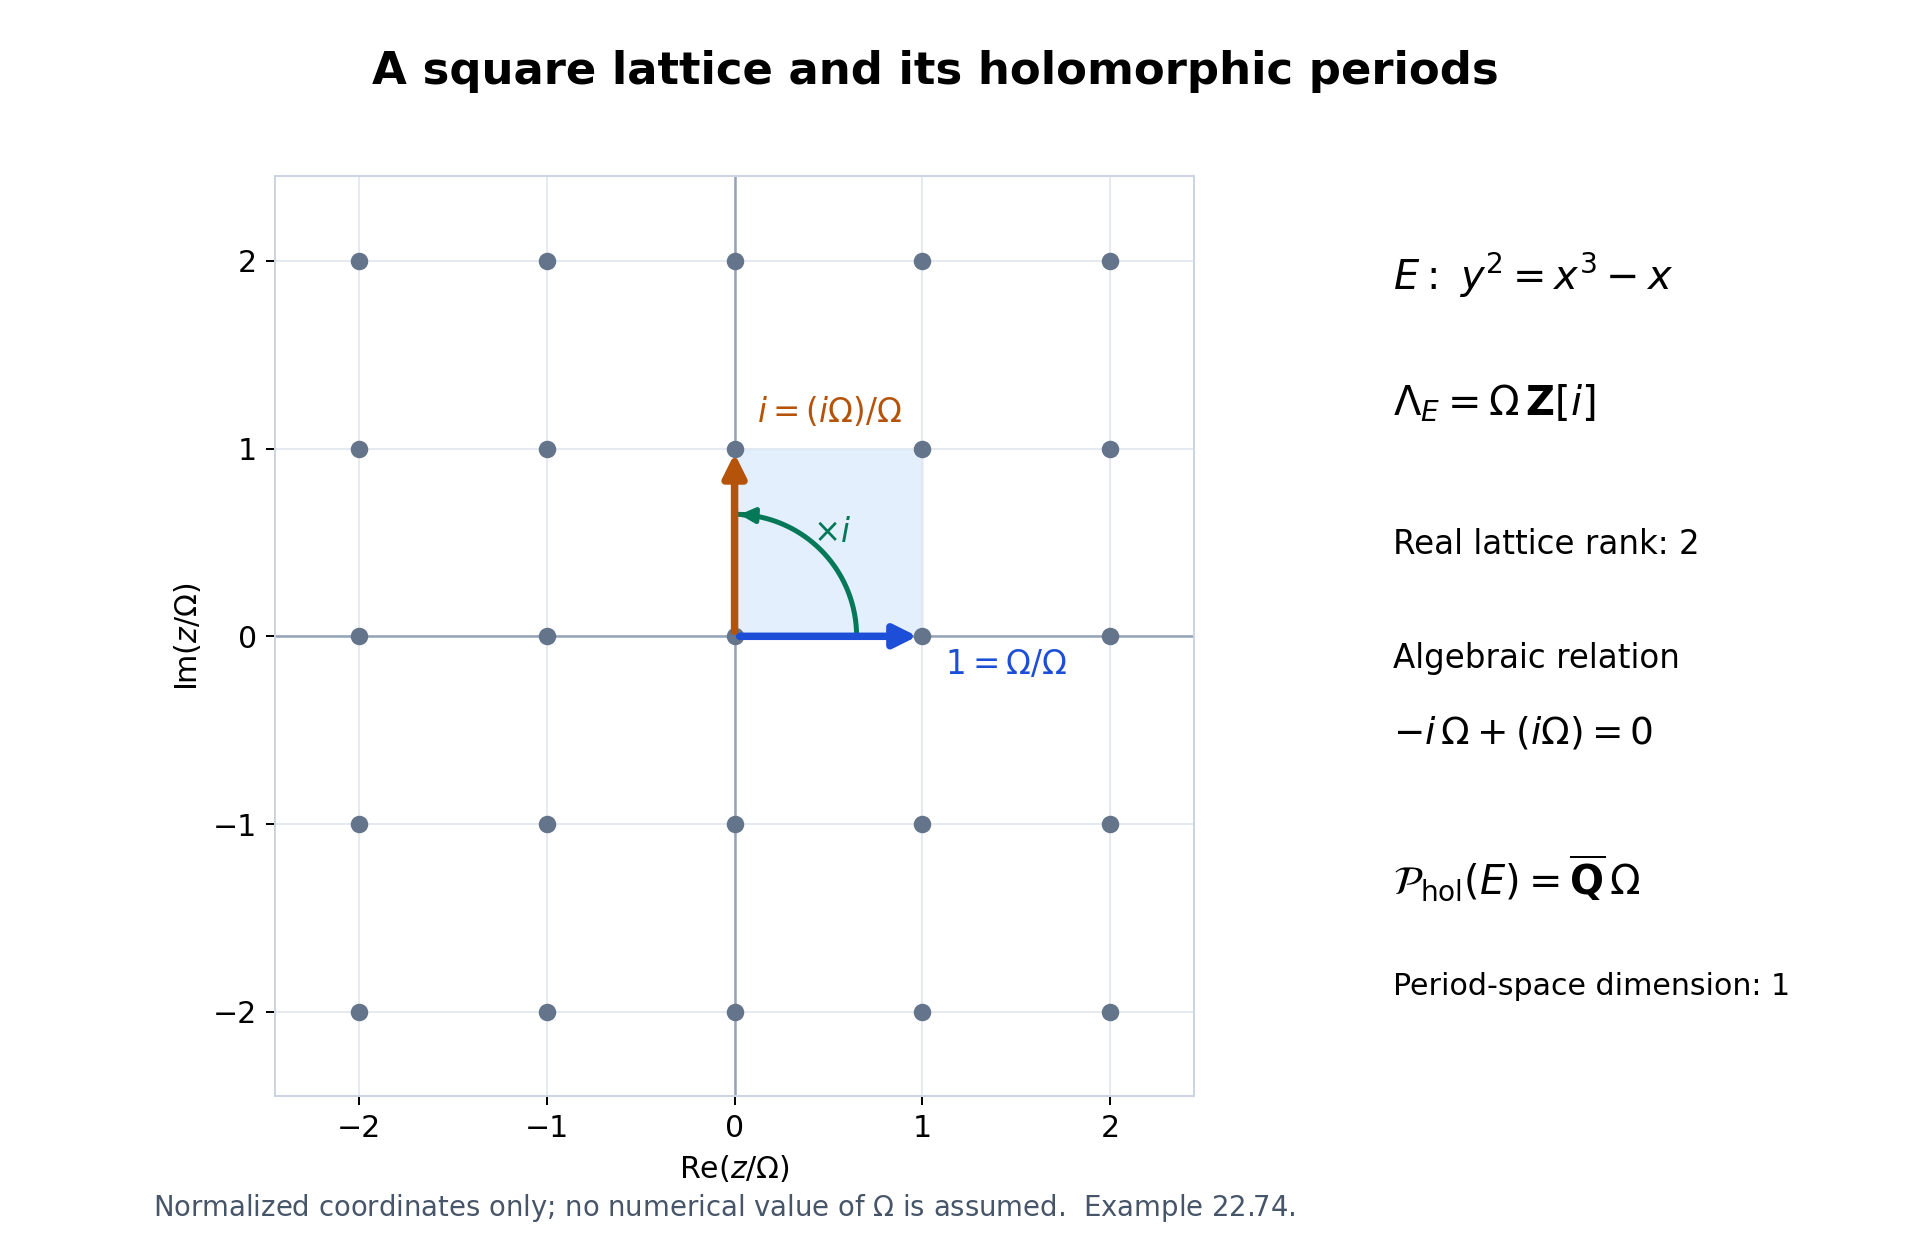
\includegraphics[keepaspectratio,alt={The period lattice after division by a generator, with its real basis and algebraic relation.}]{../verification/lesson22/cm-period-lattice.png}}
\par\smallskip
\begin{flushleft}\small
\emph{Figure 22.5. The normalized coordinate is \(z/\Omega\); the
plotted lattice points are exactly Gaussian integers in the displayed
window. Multiplication by \(i\) rotates the real basis vector \(1\) to
\(i\). Equation (22.185) explains why real lattice rank two gives
algebraic period-space dimension one. No numerical value of \(\Omega\)
is assumed.}
\end{flushleft}
\end{minipage}\par\medskip


\subsubsection{Corollary 22.75. Elliptic logarithms and changes of
branch}\label{corollary-22.75.-elliptic-logarithms-and-changes-of-branch}

Let \(E/k\) be an elliptic curve, and choose a nonzero invariant
differential to identify its Lie algebra with \(\mathbf C\). Then
\(D_E\) acts by a subfield of \(\mathbf C\) that is either \(\mathbf Q\)
or an imaginary quadratic field. Given logarithms \(u_1,\ldots,u_n\) of
algebraic points, choose a \(D_E\)-basis \(v_1,\ldots,v_r\) of their
span. Every algebraic linear relation among the \(u_j\) is obtained by
substituting their \(D_E\)-linear expressions in the \(v_a\) and setting
the resulting algebraic coefficients to zero. Moreover
\(1,v_1,\ldots,v_r\) are linearly independent over \(k\).

The intrinsic version that includes all choices of branch is \[
 U=D_Eu_1+\cdots+D_Eu_n+(\Lambda_E\otimes_{\mathbf Z}\mathbf Q),
 \qquad
 \dim_k\operatorname{span}_k U=\dim_{D_E}U.
 \tag{22.186}
\] Replacing any \(u_j\) by another logarithm of the same point leaves
\(U\) unchanged.

\textbf{Proof.} The derivative is a faithful homomorphism
\(D_E\to\mathbf C\), so \(D_E\) is commutative. Lemma 22.67 gives
rational dimension \(1\) or \(2\). If it is \(2\), it is a quadratic
field. It cannot be real: a real scalar \(c\) acting on the real plane
has matrix \(cI_2\) in every real basis. If it preserves the rational
period lattice, that matrix has rational entries in an integral lattice
basis, so \(c\in\mathbf Q\). A real quadratic subfield would contradict
this observation. Thus the quadratic case is imaginary.

Theorems 22.69 and 22.72 give the asserted independence of a basis and
of \(1\) together with that basis. On writing \(u_j=\sum_a d_{aj}v_a\),
a relation \(\sum_j b_j u_j=0\), with \(b_j\in k\), becomes
\(\sum_a(\sum_j b_jd_{aj})v_a=0\). Its coefficients vanish exactly when
the original relation holds. This is a description of all such
relations, not just a sufficient family.

For (22.186), add a finite rational basis of the period lattice to the
initial list and apply Corollary 22.70 with \(g=1\). Two logarithms of
the same point differ by a lattice vector, by the exponential covering.
This changes neither of the two containments defining \(U\). \(\square\)

\subsubsection{Exercise 22.76. Relations in a CM
example}\label{exercise-22.76.-relations-in-a-cm-example}

Let \(E,\Omega\) be as in Example 22.74. Choose \(u\) with
\(\exp_E(u)\in E(k)\) and \(u\notin\mathbf Q(i)\Omega\). Determine all
triples \((a,b,c)\in k^3\) such that \[
 a u+b(iu+\Omega)+c\Omega=0.
 \tag{22.187}
\] Then determine the dimension of the span of
\(1,2\pi i,u,iu+\Omega,\Omega\). Explain which hypothesis on the point
\(\exp_E(u)\) guarantees the stipulated condition on \(u\).

\textbf{Solution.} The vectors \(u,\Omega\) are independent over
\(\mathbf Q(i)\): a nonzero coefficient of \(u\) in a relation would
express it as a multiple of \(\Omega\), and a relation with zero
coefficient of \(u\) has zero remaining coefficient because
\(\Omega\ne0\). Theorem 22.69 therefore makes them independent over
\(k\). Equation (22.187) is \[
 (a+ib)u+(b+c)\Omega=0.
 \tag{22.188}
\] Consequently the entire relation space consists of
\((a,b,c)=b(-i,1,-1)\), \(b\in k\). Theorem 22.72 makes
\(1,2\pi i,u,\Omega\) independent, and the fifth listed number
\(iu+\Omega\) is in their span. The dimension is four.

The point \(P=\exp_E(u)\) is nontorsion if and only if
\(u\notin\Lambda_E\otimes\mathbf Q=\mathbf Q(i)\Omega\). Indeed, if
\([N]P=0\), then \(Nu\in\Lambda_E\); conversely a rational period has a
nonzero integer multiple in the lattice and therefore exponentiates to a
torsion point. This proves the precise endpoint condition, and it is
unchanged by a change of logarithm branch. \(\square\)

\subsection{Vector extensions of an abelian
variety}\label{vector-extensions-of-an-abelian-variety}

Let \(k=\overline{\mathbf Q}\), let \(A/k\) be an abelian variety, and
put \(W_A=H^1(A,\mathcal O_A)\). A vector group means a
finite-dimensional \(k\)-vector space with its additive algebraic group
structure. An extension by a vector group \(V\) is an exact sequence of
commutative algebraic groups \[
 0\longrightarrow V\longrightarrow E\longrightarrow A\longrightarrow0.
 \tag{22.189}
\] Two extensions are equivalent if their isomorphism induces the
identity on both \(V\) and \(A\). The notation
\(\operatorname{Ext}^1(A,V)\) denotes these equivalence classes, with
the addition described below.

\subsubsection{Proposition 22.77. The torsor class determines the group
extension}\label{proposition-22.77.-the-torsor-class-determines-the-group-extension}

For every vector group \(V\), passage to the underlying \(V\)-torsor
gives a natural isomorphism \[
 \operatorname{Ext}^1(A,V)\simeq W_A\otimes_k V
       \simeq\operatorname{Hom}_k(W_A^\vee,V).
 \tag{22.190}
\] Pullback along \(f:B\to A\) acts by \(f^*\otimes1\), and pushout
along a linear map \(V\to V'\) acts on the second tensor factor.

\textbf{Proof.} A vector-group torsor is trivial on an affine scheme.
The affine descent argument in the proof of Proposition 22.39 proves
this directly: the additive transition cocycle in a faithfully flat
trivialization is a boundary in the augmented Amitsur complex. Thus a
finite affine open cover of \(A\) trivializes any such torsor. Its
changes of coordinates are translations \[
 t_j=t_i+c_{ij},\qquad
 c_{ij}+c_{j\ell}=c_{i\ell},
 \quad c_{ij}\in\mathcal O_A(U_i\cap U_j)\otimes_kV.
 \tag{22.191}
\] Changing the local origins changes \(c\) by a Čech boundary.
Conversely these translations glue the products \(U_i\times V\) to a
torsor; coboundaries give its isomorphisms. Affine intersections are
acyclic for quasi-coherent sheaves, so the Čech complex computes
\(H^1\). This precise comparison, and the product-cover Künneth
calculation, are proved in
\href{https://github.com/KokunoYumeto/open-math-courses-public/blob/146dc81802e69cf262fb6cc65c1b9f74e71f4625/docs/courses/AG-GS/src/abelian-varieties.md\#611-the-picard-scheme-and-the-dual-variety}{\emph{Abelian
varieties}, Lemma 6.11}. Hence torsor classes are \(W_A\otimes V\).

Every such class \(c\) is primitive under addition \(m:A\times A\to A\):
\[
 m^*c=p_1^*c+p_2^*c.
 \tag{22.192}
\] Indeed, the same Künneth calculation identifies
\(H^1(A\times A,\mathcal O)\) with the direct sum of the two copies of
\(W_A\). Restriction to either axis is the corresponding projection. The
restrictions of \(m\) to both axes are the identity, proving (22.192).

Let \(P\to A\) represent \(c\), and choose an origin \(e\in P_0(k)\).
The sum of the two pulled-back torsors on \(A^2\) has class
\(p_1^*c+p_2^*c\). In local coordinates its transition functions are the
sums of the two transition functions. Equivalently it is the quotient of
\(P\times P\) by \((p,q)\mapsto(p+v,q-v)\). Equation (22.192) gives an
isomorphism from this torsor to \(m^*P\), hence an algebraic operation
\(\mu:P\times P\to P\) satisfying \[
 \mu(p+v,q+w)=\mu(p,q)+v+w.
 \tag{22.193}
\] The maps \(p\mapsto\mu(p,e)-p\) and \(p\mapsto\mu(e,p)-p\) descend to
regular maps \(A\to V\). They are constant, since \(A\) is connected and
proper, and their values agree at \(p=e\). Subtract that common value
from \(\mu\). Both unit identities now hold.

The difference between \(\mu(\mu(p,q),r)\) and \(\mu(p,\mu(q,r))\) is a
vector in their common fibre. Equation (22.193) makes it independent of
translations in all three variables, so it descends to a regular map
\(A^3\to V\). It is constant by properness and zero at \((e,e,e)\). Thus
\(\mu\) is associative. The commutator difference similarly descends to
a constant map \(A^2\to V\) and vanishes at \((e,e)\), proving
commutativity.

For \(p\) over \(a\), there is a unique \(q\) over \(-a\) such that
\(\mu(p,q)=e\): translation in \(q\) changes the result by exactly the
same vector. This inverse depends algebraically on \(p\), as follows
immediately in local trivializations over an open cover and its images
under \([-1]\); uniqueness glues those local inverse maps. Thus \(P\),
with identity \(e\), is a commutative algebraic group extension. Its
kernel is \(V\) by (22.193). It is smooth and connected because its base
and its vector-group fibres are smooth and connected.

Two normalized operations on the same torsor differ by a regular map
\(A^2\to V\), constant and zero at the origin, hence are equal. A torsor
isomorphism can be translated by a constant vector to send the chosen
origins to one another. After that translation it respects the uniquely
normalized group operations. This proves that the torsor class
classifies extensions.

For completeness, addition of extension classes is the following
operation: take \(E_1\times_AE_2\) and quotient its kernel \(V\times V\)
by the kernel of addition \(V\times V\to V\). Its local transition
functions are \(c^{(1)}_{ij}+c^{(2)}_{ij}\). Scalar multiplication and a
general pushout apply the scalar or linear map to these functions.
Pullback composes the cocycles with the base morphism. These
descriptions prove the linearity and naturality asserted in (22.190).
\(\square\)

\subsubsection{Theorem 22.78. The universal vector
extension}\label{theorem-22.78.-the-universal-vector-extension}

Put \(V_A=W_A^\vee\). There is a commutative algebraic group
\(A^\natural\), unique up to a unique isomorphism over \(A\), with an
extension \[
 0\longrightarrow V_A\longrightarrow A^\natural
       \xrightarrow{\pi_A}A\longrightarrow0
 \tag{22.194}
\] whose class in \(\operatorname{Hom}_k(V_A,V_A)\) is the identity. For
any vector extension \(E\to A\), there is exactly one algebraic group
homomorphism \(A^\natural\to E\) over \(A\). If \(\dim A=g\), then \[
 \dim V_A=g,\qquad \dim A^\natural=2g.
 \tag{22.195}
\]

\textbf{Proof.} Proposition 22.77 constructs the extension associated
with \(\operatorname{id}_{V_A}\). Let \(E\) be an extension by \(V\),
and let \(\beta:V_A\to V\) be its classifying map. Pushing out (22.194)
by \(\beta\) gives the class \(\beta\), hence an extension equivalent to
\(E\). The pushout map supplies the asserted homomorphism.

Any homomorphism over \(A\) restricts on the kernels to a homomorphism
\(V_A\to V\). Such a homomorphism is linear: its coordinate polynomials
satisfy \(P(x+y)=P(x)+P(y)\); differentiating in \(y\) at zero shows
that all first partial derivatives are constant in characteristic zero.
Proposition 22.77 therefore makes that restriction equal to \(\beta\).
The difference between two maps with this restriction descends to a
homomorphism \(A\to V\), which is zero by properness. This proves
uniqueness, including the uniqueness of the universal extension itself.
Finally
\href{https://github.com/KokunoYumeto/open-math-courses-public/blob/146dc81802e69cf262fb6cc65c1b9f74e71f4625/docs/courses/AG-GS/src/abelian-varieties.md\#the-representing-dual-and-its-universal-bundle}{\emph{Abelian
varieties}, Theorem 6.15} proves \(\dim W_A=g\). Smoothness of the
torsor gives the dimension formula. \(\square\)

\subsubsection{Proposition 22.79. No affine quotient and no smaller
subgroup above the
base}\label{proposition-22.79.-no-affine-quotient-and-no-smaller-subgroup-above-the-base}

Every algebraic group homomorphism from \(A^\natural\) to a connected
commutative affine group is zero. If a connected algebraic subgroup
\(H\subset A^\natural\) maps onto \(A\), then \(H=A^\natural\).

\textbf{Proof.} First consider \(h:A^\natural\to\mathbf G_a\), and let
\(\ell:V_A\to k\) be its restriction. In the pushout of (22.194) by
\(\ell\), the function induced by \(h(x)+t\) on \(A^\natural\times k\)
is well-defined: replacing \((x,t)\) by \((x+v,t-\ell(v))\) does not
change it. It is a homomorphism to \(\mathbf G_a\) whose restriction to
the kernel is the identity. Its kernel gives a splitting of that
extension; equivalently subtracting this function from the kernel
coordinate identifies the extension with \(A\times\mathbf G_a\). By
Proposition 22.77 its class is zero. But the pushout class is exactly
\(\ell\in V_A^\vee=W_A\), so \(\ell=0\). Now \(h\) descends to \(A\),
and is zero by properness.

A homomorphism \(A^\natural\to\mathbf G_m\) is trivial on \(V_A\), since
an invertible polynomial on affine space is constant and a group
homomorphism takes zero to one. It too descends to \(A\), hence is
trivial. The affine classification in Theorem 22.38 proves the assertion
for any connected commutative affine target.

Suppose \(H\to A\) is surjective. The quotient \(Q=A^\natural/H\) exists
by the commutative group quotient theorem. The map \(V_A\to Q\) is
surjective: subtract a point of \(H\) with the same image in \(A\) from
any point of \(A^\natural\). The same assertion holds as a surjection of
group schemes, by the image theorem over the algebraically closed field.
Every closed subgroup of a vector group in characteristic zero is a
vector subspace. For its identity component this is Proposition 22.37;
if a subgroup had a further component, a positive multiple of any point
in that component would lie in the identity component, forcing the point
itself into the same vector subspace. Hence \(Q\), as a quotient of
\(V_A\), is a vector group. If it were nonzero, a nonzero linear
functional on it would contradict the first assertion. Thus \(Q=0\) and
\(H=A^\natural\). \(\square\)

\subsubsection{Proposition 22.80. Functoriality, products and
isogenies}\label{proposition-22.80.-functoriality-products-and-isogenies}

Every homomorphism \(f:A\to B\) lifts uniquely to a homomorphism
\(f^\natural:A^\natural\to B^\natural\) over \(f\). Its map on vector
kernels is the dual of \(f^*:W_B\to W_A\). The lifts preserve addition,
composition and identities. Moreover, \[
 (A\times B)^\natural\simeq A^\natural\times B^\natural,
 \qquad [N]^\natural=[N].
 \tag{22.196}
\] An isogeny induces an isogeny of universal extensions.

\textbf{Proof.} Pull back \(B^\natural\to B\) along \(f\) and apply the
universal property of \(A^\natural\). The tensor description in (22.190)
identifies the kernel map with the stated dual. Uniqueness proves
compatibility with composition and identities.

The sum of two lifts is a homomorphism over the sum of the base maps,
and therefore is its unique lift. Here the sum is defined by the group
law on the target. This proves additivity and the assertion for integer
multiplication. For the product, Künneth identifies
\(W_{A\times B}=W_A\oplus W_B\). The class of
\(A^\natural\times B^\natural\) is the identity on the dual direct sum,
so Theorem 22.78 gives the first isomorphism in (22.196).

If \(f:A\to B\) is an isogeny, choose \(h:B\to A\) with \(hf=[N]\) and
\(fh=[N]\), as in Lemma 22.67. The lifted maps satisfy the same
identities. On every connected commutative group in characteristic zero,
multiplication by \(N\ne0\) is surjective with finite kernel:
surjectivity follows from the exponential of Proposition 22.35, and its
differential \(N\operatorname{id}\) makes the kernel zero-dimensional.
The image theorem turns surjectivity on complex points into algebraic
surjectivity. Thus \(f^\natural\) is surjective, and its kernel is
contained in the finite kernel of \([N]\). A surjective homomorphism
with finite kernel is a finite torsor under that kernel, hence an
isogeny. \(\square\)

\subsubsection{Proposition 22.81. Periods lift uniquely to the universal
extension}\label{proposition-22.81.-periods-lift-uniquely-to-the-universal-extension}

The differential of \(\pi_A\) induces an isomorphism of abelian groups
\[
 \Lambda_{A^\natural}\xrightarrow{\ \sim\ }\Lambda_A.
 \tag{22.197}
\] It is compatible with every homomorphism of abelian varieties and,
after tensoring with \(\mathbf Q\), with their rational endomorphisms.

\textbf{Proof.} A period in the kernel of this map lies in
\(\operatorname{Lie}V_A\). The exponential of a vector group is the
identity, so that period is zero. Conversely, let
\(\lambda\in\Lambda_A\). Lift it to
\(w\in\operatorname{Lie}A^\natural(\mathbf C)\). By functoriality of the
exponential, \(\exp_{A^\natural}(w)\) lies in \(V_A(\mathbf C)\). Regard
this point as the vector \(v\in\operatorname{Lie}V_A(\mathbf C)\). Then
\(w-v\) is a period above \(\lambda\), proving surjectivity. Uniqueness
makes the lift additive.

Functoriality follows from Proposition 22.80 and the exponential
identity. Integer denominators give the rational statement. In
particular, for simple \(A\) with \(e=\dim_{\mathbf Q}D_A\), \[
 \operatorname{rank}_{\mathbf Z}\Lambda_{A^\natural}=2g,\qquad
 \dim_{D_A}(\Lambda_{A^\natural}\otimes\mathbf Q)=\frac{2g}{e}.
 \tag{22.198}
\] Although \(A^\natural\) has complex dimension \(2g\), its period
lattice has rank \(2g\), not \(4g\). Its analytic quotient is not
compact. \(\square\)

\subsection{Linear relations among periods of the universal
extension}\label{linear-relations-among-periods-of-the-universal-extension}

Define \(\mathcal P_\natural(A)\subset\mathbf C\) to be the \(k\)-span
of the scalar coordinates of the vectors in \(\Lambda_{A^\natural}\), in
any \(k\)-basis of \(\operatorname{Lie}A^\natural\). Algebraic changes
of basis preserve this space.

\subsubsection{Theorem 22.82. The period-coordinate
dimension}\label{theorem-22.82.-the-period-coordinate-dimension}

If \(A\sim_k\prod_i A_i^{m_i}\), where the \(A_i\) are pairwise
nonisogenous simple abelian varieties of dimensions \(g_i\) and
endomorphism-algebra dimensions \(e_i\), then \[
 \dim_k\mathcal P_\natural(A)=
       \sum_i\frac{4g_i^2}{e_i}.
 \tag{22.199}
\] Multiplicity \(m_i\ge1\) does not change the summand.

\textbf{Proof.} Choose a \(D_{A_i}\)-basis \(u_{i1},\ldots,u_{ir_i}\) of
\(\Lambda_{A_i^\natural}\otimes\mathbf Q\), where \(r_i=2g_i/e_i\). Its
projection is a \(D_{A_i}\)-basis of the rational period lattice of
\(A_i\), by Proposition 22.81. Rational periods exponentiate to torsion
algebraic points: an integer multiple is a period, and the finite
multiplication fibre is defined over \(k\). Thus the analytic subgroup
theorem applies to their tuple \[
 u=(u_{ij})\in
 \operatorname{Lie}G(\mathbf C),\qquad
 G=\prod_i(A_i^\natural)^{r_i}.
 \tag{22.200}
\] Let \(H\subset G\) be its minimal algebraic Lie hull. Project to
\(P=\prod_i A_i^{r_i}\). If the image of \(H\) were proper, Lemma 22.68
would give a nonzero endomorphism relation among the projected basis
vectors, a contradiction. Its image is therefore all of \(P\).

By Proposition 22.80, \(G=P^\natural\). Proposition 22.79 now forces
\(H=G\). Theorem 22.64 consequently says that all
\(\dim G=\sum_i2g_i r_i\) scalar coordinates of the tuple \(u\) are
linearly independent over \(k\). They span all the period coordinates:
every rational period is a \(D_{A_i}\)-linear combination of the chosen
basis vectors, and the differential matrices of the lifted rational
endomorphisms have entries in \(k\). This proves (22.199) for the
product of distinct simple factors.

Products concatenate their period-coordinate lists, so repeated factors
contribute the same scalar span. Finally Proposition 22.80 lifts an
isogeny to an isogeny of universal extensions. Its invertible algebraic
differential carries one rational period lattice onto the other: reverse
isogenies give finite-index inclusions exactly as in Theorem 22.73.
Hence isogenous abelian varieties have equal spaces
\(\mathcal P_\natural\) as subspaces of \(\mathbf C\). This proves the
general assertion. \(\square\)

\subsubsection{Theorem 22.83. The additive and multiplicative
contributions}\label{theorem-22.83.-the-additive-and-multiplicative-contributions}

Let \(\ell_1,\ldots,\ell_t\) be rationally independent logarithms of
nonzero algebraic numbers. Then \[
 k+\sum_{j=1}^t k\ell_j+\mathcal P_\natural(A)
   =k\oplus\bigoplus_{j=1}^t k\ell_j\oplus\mathcal P_\natural(A).
 \tag{22.201}
\] In particular, \[
 \dim_k\bigl(k+k(2\pi i)+\mathcal P_\natural(A)\bigr)
      =2+\sum_i\frac{4g_i^2}{e_i}.
 \tag{22.202}
\]

\textbf{Proof.} Use the tuple of period basis vectors in (22.200), and
form \(z=(1,\ell_1,\ldots,\ell_t,u)\) in the Lie algebra of
\(L\times G\), where \(L=\mathbf G_a\times\mathbf G_m^t\). Let \(H\) be
its algebraic Lie hull. The argument of Theorem 22.82 forces the
projection \(H\to G\) to be surjective. Put \(K=(\ker(H\to G))^0\).
Proposition 22.37 makes \(L/K\) a connected commutative affine group.
The induced map \(f:H/K\to G\) is an isogeny.

The reverse-isogeny descent in Lemma 22.67 applies to this isogeny of
commutative algebraic groups: kill its finite kernel by an integer
\(N\), and descend multiplication by \(N\) along \(f\). We obtain
\(h:G\to H/K\) with \(hf=[N]\). The first projection induces
\(q:H/K\to L/K\). Since \(G=P^\natural\), Proposition 22.79 gives
\(qh=0\). Thus \(q[N]=qhf=0\). Surjectivity of \([N]\) gives \(q=0\).

It follows that \(H\subset K\times G\); both sides have the same
dimension and are connected, so equality holds. The additive coordinate
\(1\) forces the additive factor of \(K\) to be all of \(\mathbf G_a\).
Rational independence of the \(\ell_j\) rules out every proper torus
factor, by the integral-character argument of Theorem 22.72. Therefore
\(H=L\times G\). The analytic subgroup theorem gives linear independence
of all coordinates of \(z\), proving (22.201). Set \(t=1\),
\(\ell_1=2\pi i\), to obtain (22.202). \(\square\)

For an elliptic curve, \(g=1\) and \(e\) is \(1\) or \(2\), by Corollary
22.75. The dimensions just proved are therefore:

{\def\LTcaptype{none} % do not increment counter
\begin{longtable}[]{@{}
  >{\raggedright\arraybackslash}p{(\linewidth - 6\tabcolsep) * \real{0.2000}}
  >{\raggedleft\arraybackslash}p{(\linewidth - 6\tabcolsep) * \real{0.2667}}
  >{\raggedleft\arraybackslash}p{(\linewidth - 6\tabcolsep) * \real{0.2667}}
  >{\raggedleft\arraybackslash}p{(\linewidth - 6\tabcolsep) * \real{0.2667}}@{}}
\toprule\noalign{}
\begin{minipage}[b]{\linewidth}\raggedright
Endomorphism algebra
\end{minipage} & \begin{minipage}[b]{\linewidth}\raggedleft
\(\dim_k\mathcal P_{\mathrm{hol}}(E)\)
\end{minipage} & \begin{minipage}[b]{\linewidth}\raggedleft
\(\dim_k\mathcal P_\natural(E)\)
\end{minipage} & \begin{minipage}[b]{\linewidth}\raggedleft
Dimension after adjoining \(1,2\pi i\)
\end{minipage} \\
\midrule\noalign{}
\endhead
\bottomrule\noalign{}
\endlastfoot
\(\mathbf Q\) & \(2\) & \(4\) & \(6\) \\
An imaginary quadratic field & \(1\) & \(2\) & \(4\) \\
\end{longtable}
}

The first column of dimensions uses holomorphic integrals as defined in
(22.179). The second uses the period vectors of the group (22.194). Each
definition specifies both the algebraic coordinate structure and the
paths or exponential kernel involved.

\subsection{Algebraic differential forms and period
vectors}\label{algebraic-differential-forms-and-period-vectors}

For a smooth separated variety \(X/k\), write
\(H^q_{\mathrm{dR}}(X/k)=\mathbb H^q(X,\Omega^\bullet_{X/k})\). One
computes this group with the total Čech--de Rham complex of a finite
affine cover. Intersections in this cover are affine, and
differential-form sheaves are quasi-coherent; the affine acyclicity and
Čech comparison used in Proposition 22.77 apply degree by degree.

In degree one a cocycle consists of regular one-forms \(\alpha_i\) on
\(U_i\) and regular functions \(f_{ij}\) on intersections, with \[
 d\alpha_i=0,\qquad
 \alpha_j-\alpha_i=df_{ij},\qquad
 f_{ij}+f_{j\ell}=f_{i\ell}.
 \tag{22.203}
\] A boundary has the form \((dg_i,g_j-g_i)\). Refining the cover gives
the same cohomology.

\subsubsection{Lemma 22.84. Vector torsors preserve algebraic de Rham
cohomology}\label{lemma-22.84.-vector-torsors-preserve-algebraic-de-rham-cohomology}

If \(p:Y\to X\) is a torsor under a vector bundle on a smooth separated
variety over a field of characteristic zero, then pullback induces
isomorphisms \[
 p^*:H^q_{\mathrm{dR}}(X/k)\xrightarrow{\;\sim\;}
       H^q_{\mathrm{dR}}(Y/k)\qquad(q\ge0).
 \tag{22.204}
\]

\textbf{Proof.} Choose a finite affine cover trivializing both the
vector bundle and the torsor. The latter is possible by the additive
affine-descent argument of Proposition 22.39. The preimage of every
intersection is a product with affine space, and is therefore affine.

On such an intersection write the coordinate ring of the base as \(R\)
and the fibre coordinates as \(t_1,\ldots,t_r\). The complex of absolute
differentials of \(R[t_1,\ldots,t_r]/k\) is the tensor product of the
differential complexes of \(R/k\) and \(k[t_1,\ldots,t_r]/k\), with the
total-degree signs. Give each \(t_j\) and \(dt_j\) weight one and each
base form weight zero. Let \[
 D=\sum_{j=1}^r t_j\frac{\partial}{\partial t_j}.
\] Contraction \(\iota_D\) is a derivation of form degree \(-1\),
vanishes on base forms and satisfies \(\iota_D(dt_j)=t_j\). On a
homogeneous form \(\beta\) of fibre weight \(m\), direct application of
the product rule gives \[
 (d\iota_D+\iota_Dd)\beta=m\beta.
 \tag{22.205}
\] Indeed the identity holds on functions from \(R\), their
differentials, and on \(t_j,dt_j\); both sides are degree-zero
derivations, so it holds on every product. For \(m>0\), division by
\(m\) contracts that weight subcomplex. Weight zero is exactly the
complex of base forms. Thus pullback is a quasi-isomorphism on each
affine intersection.

These pullbacks commute with restrictions, although the chosen
contractions need not. Apply them to the two Čech--de Rham double
complexes. Filtering the mapping cone by Čech degree gives acyclic
columns by the preceding calculation. This implies that its total
complex is acyclic: for a total cocycle, remove its component of
smallest Čech degree by a primitive in that column; subtract the
resulting total boundary and continue to the next column. The finite
cover bounds the number of columns. Consequently the map on total
cohomology is an isomorphism, proving (22.204). \(\square\)

\subsubsection{Theorem 22.85. Invariant forms on the universal
extension}\label{theorem-22.85.-invariant-forms-on-the-universal-extension}

There is a natural \(k\)-linear isomorphism \[
 \Theta_A:\operatorname{Lie}(A^\natural)^\vee
       \xrightarrow{\;\sim\;}H^1_{\mathrm{dR}}(A/k).
 \tag{22.206}
\] It sends an invariant one-form \(\theta\) on \(A^\natural\) to the
unique class whose pullback is \([\theta]\). Under this isomorphism, the
subspace of forms pulled back from \(A\) is \(H^0(A,\Omega^1_{A/k})\).

\textbf{Proof.} A covector at the identity of a smooth group extends
uniquely to an invariant regular one-form: at a point \(x\), transport
it by the differential of translation by \(-x\). The group law makes
this construction algebraic. On a commutative group every invariant
one-form is closed. To see this, evaluate \(d\theta\) on invariant
vector fields \(X,Y\): \[
 d\theta(X,Y)=X(\theta(Y))-Y(\theta(X))-\theta([X,Y])=0.
\] The first two functions are constant and the bracket is zero.
Invariant vector fields span every tangent space, proving the assertion.

Lemma 22.84 applies to \(\pi_A:A^\natural\to A\), so
\(\Theta_A=(\pi_A^*)^{-1}[\theta]\) is defined. We first prove
injectivity. If the class of a global closed one-form is zero in the
Čech--de Rham complex, then it is \(dF\) for a global regular function
\(F\): a total degree-zero primitive is a list of local functions, and
its vanishing Čech component says precisely that they glue.

Suppose therefore that \(\theta=dF\) is invariant on \(A^\natural\). For
every \(x\in A^\natural(k)\), \[
 d\bigl(F(x+z)-F(z)\bigr)=0.
 \tag{22.207}
\] A regular function with zero differential on a connected smooth
variety over \(k\) is constant. Indeed, on an irreducible component, a
nonconstant rational function \(F\) is transcendental over the
algebraically closed field \(k\). Extend \(F\) to a transcendence basis
of its function field. The derivation that sends \(F\) to \(1\) and the
other basis elements to zero extends through the remaining finite
separable extension: for an algebraic generator with minimal polynomial
\(P\), the forced value is \(-D(P)(a)/P'(a)\), where \(D(P)\)
differentiates coefficients. Since \(P'(a)\ne0\), this defines the
extension and rules out \(dF=0\). Connected smooth algebraic groups are
irreducible, as in Proposition 22.35. Evaluating (22.207) at \(z=0\)
therefore gives \[
 F(x+z)-F(0)=(F(x)-F(0))+(F(z)-F(0)).
\] Equality on algebraic points is equality of morphisms over the
algebraically closed field. Thus \(F-F(0)\) is a homomorphism
\(A^\natural\to\mathbf G_a\). Proposition 22.79 makes it zero, so
\(\theta=0\).

Both sides of (22.206) have dimension \(2g\). For the left side this is
Theorem 22.78. For the right side,
\href{https://github.com/KokunoYumeto/open-math-courses-public/blob/146dc81802e69cf262fb6cc65c1b9f74e71f4625/docs/courses/AG-GS/src/abelian-varieties.md\#the-other-mapped-chapter-vii-consequences}{\emph{Abelian
varieties}, Propositions 6.40--6.41} prove \[
 0\longrightarrow H^0(A,\Omega^1_{A/k})
 \longrightarrow H^1_{\mathrm{dR}}(A/k)
 \longrightarrow H^1(A,\mathcal O_A)\longrightarrow0,
 \tag{22.208}
\] whose outer terms have dimension \(g\). In characteristic zero the
degeneration step also follows directly from the integer weights in
Proposition 6.40: on the Hodge spectral sequence \([2]^*\) has weight
\(2^{p+q}\) at \((p,q)\), whereas a differential raises total degree by
one. Commutation with \([2]^*\) forces every differential to vanish,
inductively from the first page. Injectivity and equality of dimensions
prove (22.206).

Every global regular one-form on \(A\) is invariant: translation
trivializes its cotangent bundle, and its coefficient functions are
constant by properness. Pullback to \(A^\natural\) is invariant and
represents its ordinary de Rham class. This proves the subspace
assertion. Pullback of forms, the torsor isomorphism (22.204), and the
unique lifted homomorphisms of Proposition 22.80 commute, proving
naturality. \(\square\)

\subsubsection{Proposition 22.86. The integral is the lifted period
coordinate}\label{proposition-22.86.-the-integral-is-the-lifted-period-coordinate}

For \(\lambda\in\Lambda_A\), let \(\lambda^\natural\) be its unique lift
in \(\Lambda_{A^\natural}\), and let
\(\gamma_\lambda(t)=\exp_A(t\lambda)\), \(0\le t\le1\). Then \[
 \int_{\gamma_\lambda}\Theta_A(\theta)
       =\theta(\lambda^\natural).
 \tag{22.209}
\] The left side is the integral of a de Rham class, defined from
(22.203).

\textbf{Proof.} Subdivide a closed piecewise smooth path into arcs
\(\gamma_j\) contained in \(U_{i_j}(\mathbf C)\). Put \(i_{s+1}=i_1\),
and denote the endpoint of \(\gamma_j\) by \(x_j\). For a cocycle
(22.203), its integral is \[
 \sum_{j=1}^s\int_{\gamma_j}\alpha_{i_j}
       +\sum_{j=1}^s f_{i_j i_{j+1}}(x_j).
 \tag{22.210}
\] The plus sign in the second sum is essential. For a boundary
\((dg_i,g_j-g_i)\), the arc integrals telescope to the negative of that
second sum, giving zero.

Refining an arc does not change the answer. Replacing its index \(i\) by
\(j\) changes the arc integral by
\(f_{ij}(\mathrm{end})-f_{ij}(\mathrm{start})\); the changes at its two
transitions cancel these terms, using the cocycle identity. A common
refinement therefore proves independence of all cover choices. The same
calculation proves compatibility with pullback.

The integral depends only on the homotopy class of the loop. Subdivide a
homotopy square into small rectangles mapped into members of the cover.
A closed one-form has zero integral around each such rectangle: in
coordinates this is the fundamental theorem of calculus applied to the
equality of the mixed coefficients of \(d\alpha=0\). Sum over the
rectangles. Interior edge integrals cancel, and changing indices along
edges introduces endpoint terms that cancel by the Čech identity. This
leaves equality of the two boundary-loop integrals.

The loop \(\gamma^\natural(t)=\exp_{A^\natural}(t\lambda^\natural)\)
projects to \(\gamma_\lambda\). By (22.206), the pullback of
\(\Theta_A(\theta)\) is represented by the global form \(\theta\). The
pullback of \(\theta\) to \(\operatorname{Lie}A^\natural(\mathbf C)\)
under the exponential is the constant one-form with value \(\theta\),
since it is translation invariant and the exponential has differential
the identity at zero. Its integral along the segment
\(t\lambda^\natural\) is \(\theta(\lambda^\natural)\). Pullback
compatibility of (22.210) proves (22.209).

Every based loop in \(A(\mathbf C)\) is homotopic to one of the loops
\(\gamma_\lambda\). Lift it through the exponential covering of
Proposition 22.35; its endpoints differ by \(\lambda\), and a linear
homotopy in the covering vector space joins that lift to \(t\lambda\),
fixing endpoints. An unbased loop is conjugate to a based loop by a
path, whose forward and reverse integrals cancel. Finally any finite
one-cycle can be decomposed into loops by joining its finitely many
vertices to a base point; the auxiliary paths cancel in the resulting
sum. Thus (22.209) accounts for all closed one-cycle integrals.
\(\square\)

\subsubsection{Theorem 22.87. The full pure abelian period
dimension}\label{theorem-22.87.-the-full-pure-abelian-period-dimension}

Let \(\mathcal P_{\mathrm{dR}}(A)\) be the \(k\)-span of all integrals
of classes in \(H^1_{\mathrm{dR}}(A/k)\) over closed integral one-cycles
in \(A(\mathbf C)\). If \(A\sim_k\prod_iA_i^{m_i}\), with simple
pairwise nonisogenous \(A_i\), then \[
 \mathcal P_{\mathrm{dR}}(A)=\mathcal P_\natural(A),\qquad
 \dim_k\mathcal P_{\mathrm{dR}}(A)
       =\sum_i\frac{4g_i^2}{e_i},
 \tag{22.211}
\] and \[
 \dim_k\bigl(k+k(2\pi i)+\mathcal P_{\mathrm{dR}}(A)\bigr)
       =2+\sum_i\frac{4g_i^2}{e_i}.
 \tag{22.212}
\] More generally the direct-sum assertion (22.201) holds with
\(\mathcal P_{\mathrm{dR}}(A)\) in place of \(\mathcal P_\natural(A)\).

\textbf{Proof.} By Theorem 22.85 every de Rham class is
\(\Theta_A(\theta)\). Proposition 22.86 identifies its integrals with
the values of \(\theta\) on lifted lattice vectors. Conversely every
scalar coordinate of such a vector is its value under a coordinate
covector defined over \(k\), hence is an integral. This proves equality
of the two scalar spaces. Theorems 22.82--22.83 give their dimensions
and the direct-sum assertion. \(\square\)

The factor \(4g_i^2/e_i\) includes both the holomorphic part and the
other degree-one de Rham classes. Restricting to holomorphic forms gives
the smaller formula \(2g_i^2/e_i\) of Theorem 22.73. Repeated isogeny
factors still do not add new scalar periods.

\begin{minipage}[t]{\linewidth}
\centering
\pandocbounded{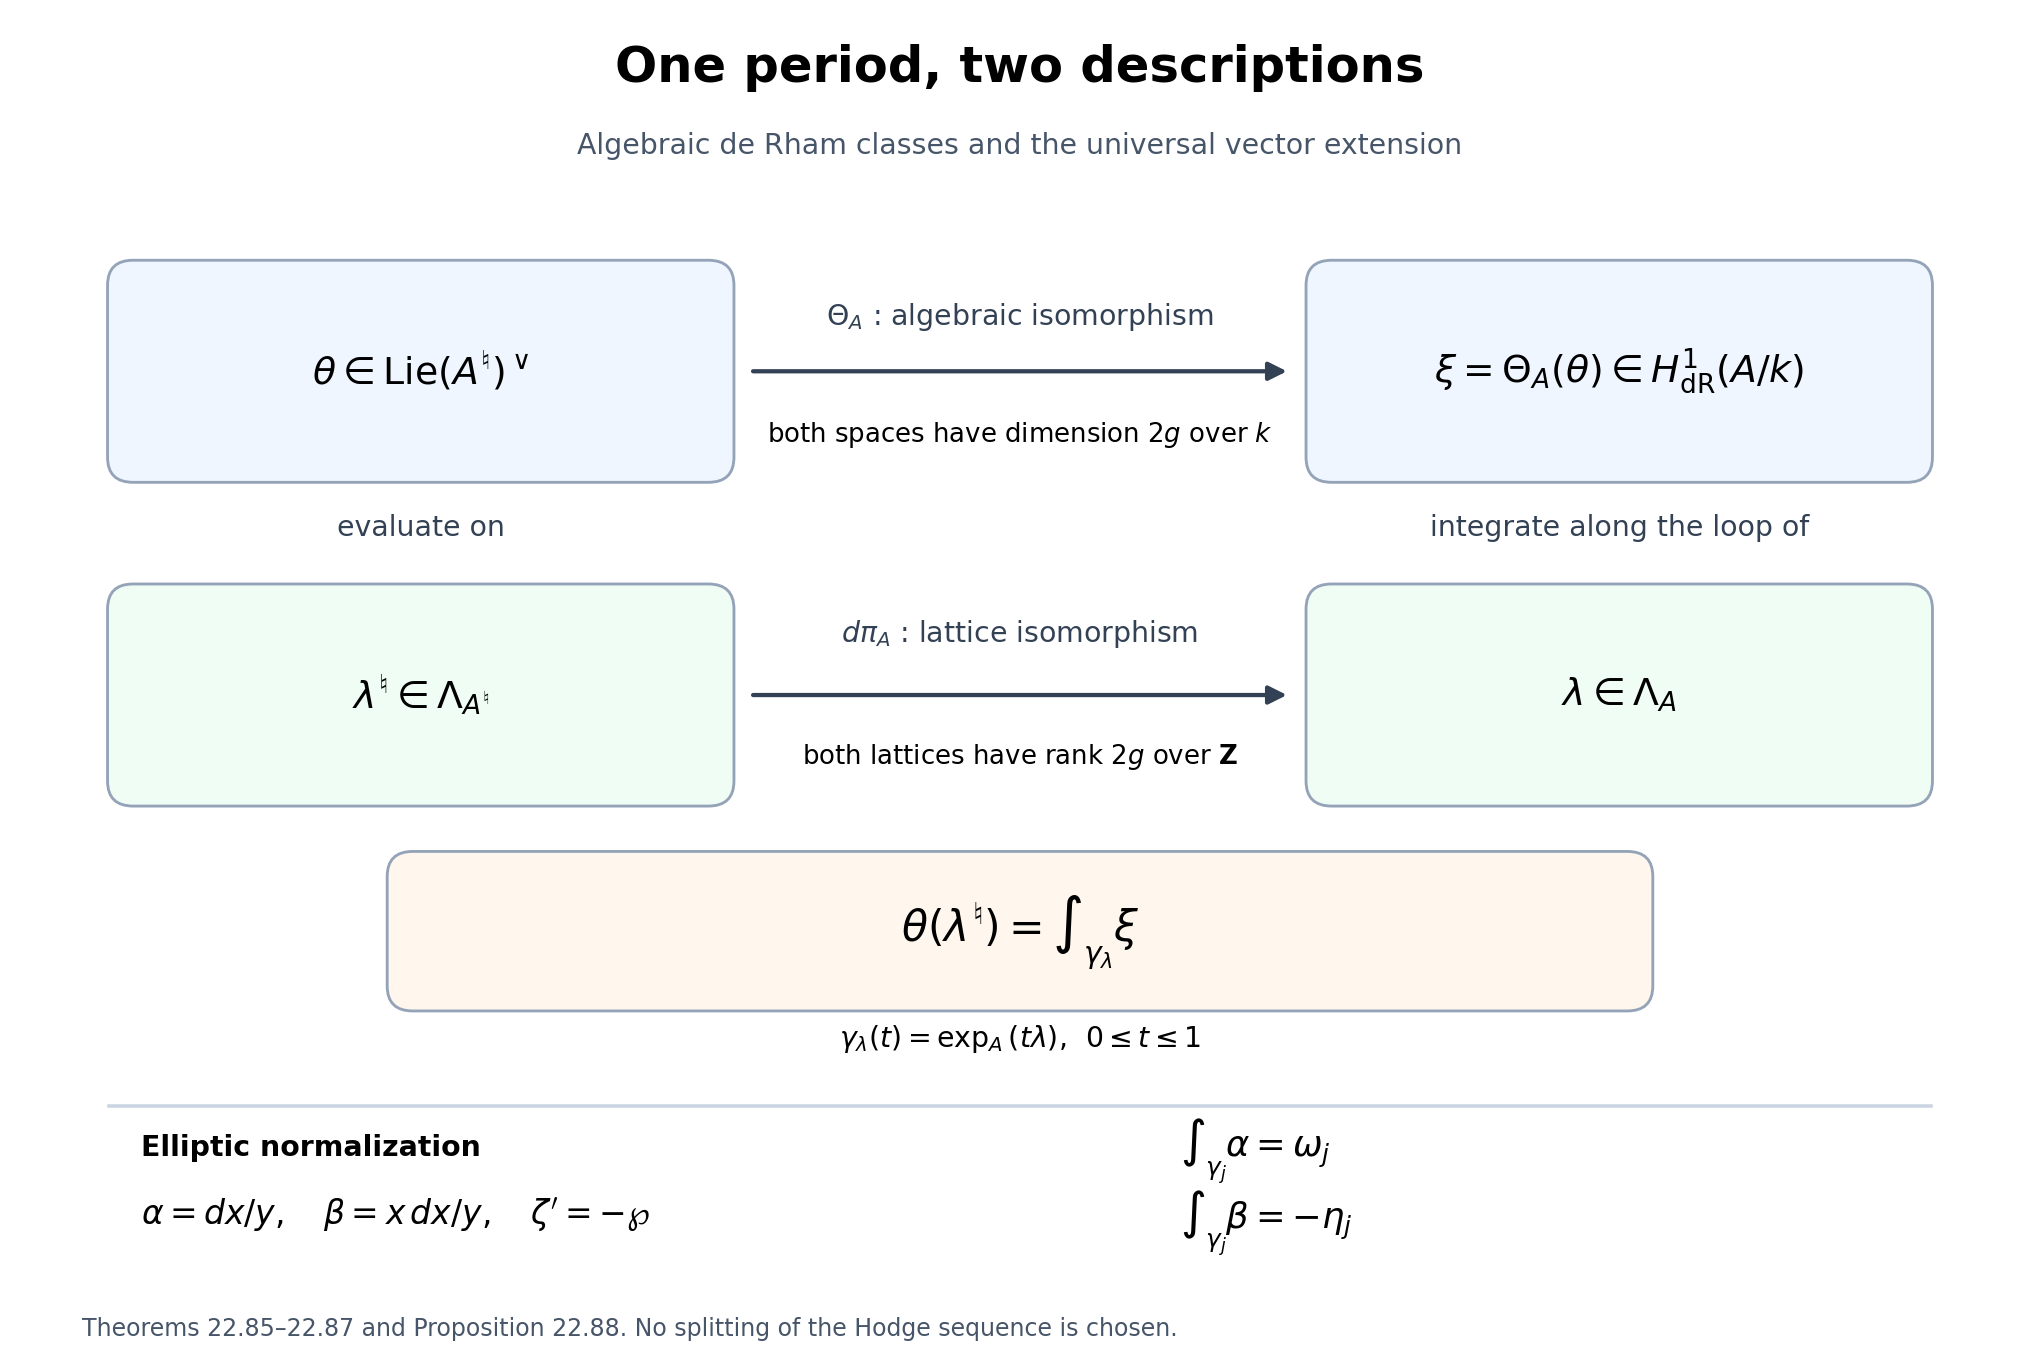
\includegraphics[keepaspectratio,alt={Invariant forms and lifted lattice vectors give the same period integrals; the elliptic period matrix includes the negative quasi-periods.}]{../verification/lesson22/universal-period-comparison.png}}
\par\smallskip
\begin{flushleft}\small
\emph{Figure 22.6. Theorem 22.85 identifies algebraic de Rham classes
with invariant covectors on the universal extension. Proposition 22.86
identifies their integrals with evaluation on the uniquely lifted period
lattice. The vector-group fibre has dimension \(g\), while both period
lattices have rank \(2g\). For an elliptic curve in the normalization of
Proposition 22.88, the two rows of the integral matrix are the periods
and the negative quasi-periods. The diagram records maps and dimensions,
without choosing a splitting of (22.208).}
\end{flushleft}
\end{minipage}\par\medskip


\subsubsection{Proposition 22.88. First- and second-kind elliptic
differentials}\label{proposition-22.88.-first--and-second-kind-elliptic-differentials}

Let \[
 E:\quad y^2=4x^3-g_2x-g_3,\qquad
 g_2,g_3\in k,\quad g_2^3-27g_3^2\ne0,
 \qquad
 \alpha=\frac{dx}{y},\quad \beta=x\frac{dx}{y}.
 \tag{22.213}
\] The classes of \(\alpha,\beta\) form a \(k\)-basis of
\(H^1_{\mathrm{dR}}(E/k)\). Here \(\beta\), which has a pole at the
identity \(O\), represents a class by cancelling its local principal
part. For a period basis \(\omega_1,\omega_2\) and the quasi-periods
\(\eta_j=\zeta(z+\omega_j)-\zeta(z)\) in the Weierstrass normalization
\(\zeta'=-\wp\), the corresponding integral matrix is \[
 \begin{pmatrix}
 \int_{\gamma_1}\alpha&\int_{\gamma_2}\alpha\\
 \int_{\gamma_1}\beta&\int_{\gamma_2}\beta
 \end{pmatrix}
 =
 \begin{pmatrix}\omega_1&\omega_2\\-\eta_1&-\eta_2\end{pmatrix}.
 \tag{22.214}
\] Consequently \[
 \dim_k\langle\omega_1,\omega_2,\eta_1,\eta_2\rangle_k
 =\frac4{\dim_{\mathbf Q}\operatorname{End}^0(E)}.
 \tag{22.215}
\]

\textbf{Proof.} The affine form \(dx/y\) is regular even where \(y=0\):
differentiating the cubic gives \(dx/y=2\,dy/(12x^2-g_2)\), whose
denominator is nonzero at those points by nonsingularity.

At \(O=[0:1:0]\) use \(q=X/Y,r=Z/Y\). The equation is
\(r=4q^3-g_2qr^2-g_3r^3\), so \(q\) is a local parameter and
\(r=4q^3+\cdots\). Put \(t=-2q=-2x/y\). Substituting \(y=-2x/t\) into
the affine equation yields \[
 t^{-2}=x-\frac{g_2}{4x}-\frac{g_3}{4x^2}.
\] It follows that \[
 x=t^{-2}+O(t^2),\quad y=-2t^{-3}+O(t),\quad
 \alpha=(1+O(t^4))\,dt,\quad
 \beta=(t^{-2}+O(t^2))\,dt.
 \tag{22.216}
\] Thus \(\alpha\) is regular everywhere and \(\beta\) has just a double
pole at \(O\), of residue zero.

Set \(h=-1/t=y/(2x)\). On a sufficiently small affine Zariski
neighbourhood \(V\) of \(O\), excluding the other poles of \(h\), the
form \(\beta-dh\) is regular. On \(U=E\setminus\{O\}\), the form
\(\beta\) is regular. The data \[
 \alpha_U=\beta,\qquad \alpha_V=\beta-dh,\qquad f_{UV}=-h
 \tag{22.217}
\] satisfy (22.203), so define its de Rham class. This is the local
construction for any differential of the second kind on a smooth curve:
integrate each finite negative Laurent principal part, which is possible
exactly when the residue term vanishes; subtract its differential and
use those rational principal parts as the Čech functions.

The two classes are independent. If \(a[\alpha]+b[\beta]=0\), its
restriction to the affine \(U\) says that \(a\alpha+b\beta=df\) for a
regular function \(f\) on \(U\). A pole of a rational function of order
\(n>0\) gives a pole of order \(n+1\) in its differential, in
characteristic zero. Thus if \(b\ne0\), \(f\) has a simple pole at \(O\)
and no other pole. But every regular function on \(U\) has a unique
expression \(P(x)+yQ(x)\), with \(P,Q\in k[x]\). The possible
nonconstant pole orders of \(P(x)\) are even and at least two; those of
\(yQ(x)\) are odd and at least three. Their leading poles cannot cancel.
A simple pole is impossible. If \(b=0\), \(df=a\alpha\) has no poles, so
\(f\) has none, and properness gives \(f\in k\). Hence \(a=0\).
Dimension two from (22.208) proves the basis assertion.

The Weierstrass uniformization and the identities
\((x,y)=(\wp(z),\wp'(z))\), \(\zeta'=-\wp\), with constant additive
quasi-periods, are proved in
\href{../TR-TRANS/TR-TRANS-08.html\#3-entire-quotients-of-strict-order-two}{\emph{Weierstrass
functions, elliptic values and periods}, Sections 1--3 and 5}. Their
pullbacks give \(\alpha=dz\) and \(\beta=\wp(z)\,dz=-d\zeta(z)\). Choose
representatives of the two cycles avoiding \(O\); their integrals are
\(\omega_j\) and \(-\eta_j\). Formula (22.210), with (22.217), makes
these the integrals of the de Rham classes, independently of
representatives. This proves (22.214). Theorem 22.87 gives (22.215).
\(\square\)

\subsubsection{Exercise 22.89. A CM curve and its second-kind
direction}\label{exercise-22.89.-a-cm-curve-and-its-second-kind-direction}

For \(E:y^2=4x^3-4x\), let \(\iota(x,y)=(-x,iy)\). Choose a lattice
generator \(\Omega\) with \(\Lambda_E=\Omega\mathbf Z[i]\), and put
\(Q=\int_{\gamma_\Omega}\beta\). Determine all linear relations over
\(k\) among the four entries of (22.214), and the dimension after
adjoining \(1,2\pi i\).

\textbf{Solution.} The square-lattice assertion follows from the
Gaussian-lattice argument of Example 22.74, which is unchanged by this
algebraic scaling of the cubic. Direct calculation gives \[
 \iota^*\alpha=i\alpha,\qquad
 \iota^*\beta=-i\beta.
 \tag{22.218}
\] The image of \(\gamma_\Omega\) under \(\iota\) represents
\(\gamma_{i\Omega}\). Hence the four matrix entries, in row order, are
\[
 (\Omega,i\Omega,Q,-iQ).
 \tag{22.219}
\] This curve has \(\operatorname{End}^0(E)=\mathbf Q(i)\), by Corollary
22.75 and the displayed automorphism. Theorem 22.87 gives dimension two,
so \(\Omega,Q\) are linearly independent over \(k\). Thus the complete
relation space consists of \((a,b,c,d)\in k^4\) satisfying \(a+ib=0\),
\(c-id=0\), and has basis \((-i,1,0,0)\), \((0,0,i,1)\). Equation
(22.212) shows that \(1,2\pi i,\Omega,Q\) are linearly independent and
span the enlarged period space, of dimension four. The relations concern
linear dependence; no assertion of algebraic independence is needed.

The algebraic identification in (22.206) and its integration
normalization are also described in Tiago J. Fonseca and Nils Matthes,
\href{https://arxiv.org/abs/2201.06402}{\emph{A note on the Gauss--Manin
connection for abelian schemes}}, Sections 2.2--2.4. Here the degree-one
comparison follows from the explicit torsor contraction, the absence of
additive quotients and the period-lifting argument above.

\subsection{Lattices, semiabelian groups and relative
periods}\label{lattices-semiabelian-groups-and-relative-periods}

A semiabelian variety over \(k=\overline{\mathbf Q}\) is a commutative
algebraic group in an exact sequence \[
 0\longrightarrow T\longrightarrow G\longrightarrow A\longrightarrow0,
 \qquad T\simeq\mathbf G_m^t,
 \tag{22.220}
\] with \(A\) an abelian variety. A \textbf{1-motive} is a homomorphism
\(M=[L\xrightarrow{u}G]\), where \(L\) is a free abelian group of finite
rank and \(u(L)\subset G(k)\). A morphism consists of compatible
homomorphisms on the lattice and on the algebraic group. We also allow
rational multiples of these morphisms, or, equivalently, work up to
isogeny. A finite-index change of lattice or an isogeny of groups then
gives the same object.

Here \(L\) records endpoints of paths as well as relations between them.
It need not inject into \(G(k)\).

\subsubsection{Lemma 22.90. Vector extensions of a torus split
uniquely}\label{lemma-22.90.-vector-extensions-of-a-torus-split-uniquely}

Every extension of a torus \(T\) by a vector group \(V\) has a unique
splitting. Moreover \(\operatorname{Hom}(T,V)=0\).

\textbf{Proof.} The affine torsor argument of Proposition 22.39 gives an
algebraic section of the underlying vector torsor. Translate it so that
its value at \(1\) is the identity. In the resulting coordinates the
group operation is \[
 (x,v)(y,w)=(xy,v+w+c(x,y)),
 \tag{22.221}
\] where \(c\) is a vector-valued Laurent polynomial on \(T^2\), zero
when either argument is \(1\). Associativity says \[
 c(x,y)+c(xy,z)=c(y,z)+c(x,yz).
 \tag{22.222}
\] Let \(F(x)\) be the coefficient of \(z^0\) in \(c(x,z)\). Taking that
coefficient in (22.222) gives \[
 c(x,y)=F(x)+F(y)-F(xy).
 \tag{22.223}
\] Indeed the constant coefficient of \(c(x,yz)\), as a Laurent
polynomial in \(z\), is \(F(x)\). Also \(F(1)=0\). The change of fibre
coordinate \(v'=v+F(x)\) turns (22.221) into the product operation.

A homomorphism \(T\to\mathbf G_a\) is a Laurent polynomial \(P\)
satisfying \(P(xy)=P(x)+P(y)\). For every nonzero character exponent
\(m\), comparison of the monomial \(x^my^m\) forces its coefficient in
\(P\) to be zero. The constant coefficient is zero too. Coordinatewise
this proves \(\operatorname{Hom}(T,V)=0\), which also proves uniqueness
of a splitting. \(\square\)

\subsubsection{Proposition 22.91. The universal vector extension of a
semiabelian
group}\label{proposition-22.91.-the-universal-vector-extension-of-a-semiabelian-group}

For (22.220), pullback induces \[
 \operatorname{Ext}^1(A,V)\simeq\operatorname{Ext}^1(G,V).
 \tag{22.224}
\] Consequently \[
 G^\natural=G\times_A A^\natural,\qquad
 0\longrightarrow V_A\longrightarrow G^\natural
 \longrightarrow G\longrightarrow0
 \tag{22.225}
\] is universal for vector extensions of \(G\). There is no nonzero
homomorphism from \(G\), or from \(G^\natural\), to a vector group.

\textbf{Proof.} If \(E\) is a vector extension of \(G\), its restriction
to \(T\) has a unique group section by Lemma 22.90. Quotient \(E\) by
the image of that section. The result is a vector extension of \(A\),
and its pullback to \(G\) is \(E\). To verify the latter assertion, the
natural map \[
 E\longrightarrow G\times_A(E/T)
\] is the identity on the vector kernel and on the quotient \(G\); in
local vector-torsor charts it is therefore an isomorphism. Conversely
the pullback of an extension of \(A\) has its canonical section over
\(T\). Uniqueness of that section makes the two operations inverse also
on isomorphisms. This proves (22.224), compatibly with Baer sums and
pushout.

A map \(G\to V\) is zero on \(T\) by Lemma 22.90, hence descends to the
proper variety \(A\) and is zero. The classification (22.224), followed
by Proposition 22.77, gives the universal property of (22.225). The
argument of Proposition 22.79 for a map to \(\mathbf G_a\) applies
unchanged: its restriction to \(V_A\) is a linear functional, the
associated pushout has a retraction and is split, and (22.224) makes
that functional zero. The map then descends to \(G\). Apply this
coordinatewise for any vector target. \(\square\)

\subsubsection{Theorem 22.92. A universal extension that remembers the
endpoints}\label{theorem-22.92.-a-universal-extension-that-remembers-the-endpoints}

There is a vector extension \(E(M)\to G\) with a specified lift
\(\widetilde u:L\to E(M)(k)\), universal among vector extensions of
\(G\) equipped with such a lift. The lift \(\widetilde u\) is injective.
If \(r=\operatorname{rank}L\), \(g=\dim A\), and \(t=\dim T\), then \[
 \dim E(M)=r+2g+t,\qquad
 \dim\ker(E(M)\to G)=r+g.
 \tag{22.226}
\]

\textbf{Proof.} Put \(L_k=L\otimes_{\mathbf Z}k\). Choose lifts to
\(G^\natural(k)\) of the images of a basis of \(L\), and extend
additively to \(v:L\to G^\natural(k)\). Define \[
 E(M)=G^\natural\times L_k,\qquad
 \widetilde u(\ell)=(v(\ell),\ell\otimes1).
 \tag{22.227}
\] Its projection to \(G\) uses the first factor. Its kernel is
\(V_A\oplus L_k\), and its lattice lift is injective by the second
coordinate.

Let \(E'\to G\) be a vector extension by \(V\), with a lift
\(u':L\to E'(k)\). There is a unique homomorphism
\(\psi:G^\natural\to E'\) over \(G\), by Proposition 22.91. The
difference \(u'(\ell)-\psi(v(\ell))\) lies in \(V(k)\) and is additive
in \(\ell\). It extends uniquely to a \(k\)-linear map
\(\delta:L_k\to V\). Then \[
 (x,a)\longmapsto\psi(x)+\delta(a)
 \tag{22.228}
\] is the required map \(E(M)\to E'\). Every such map must equal
\(\psi\) on \(G^\natural\), and its restriction to \(L_k\) is linear and
forced by the values on the lattice. This proves uniqueness. It also
gives a unique isomorphism between constructions made with different
choices of \(v\). The dimensions follow from (22.225).

For a morphism \(f:M\to N\), pull back \(E(N)\) along its group map and
use its lattice lift. The same universal property gives a unique
\(E(f):E(M)\to E(N)\). Uniqueness proves composition, identities and
additivity. Thus the construction is functorial, even though the product
description (22.227) depends on choices. \(\square\)

\subsubsection{Proposition 22.93. Exactness of the universal
extensions}\label{proposition-22.93.-exactness-of-the-universal-extensions}

Suppose \[
 0\longrightarrow M_1\longrightarrow M
 \longrightarrow M_2\longrightarrow0
 \tag{22.229}
\] is represented by exact lattice and semiabelian-group sequences, with
free lattice quotient and connected group kernel. Then \[
 0\longrightarrow E(M_1)\longrightarrow E(M)
 \longrightarrow E(M_2)\longrightarrow0
 \tag{22.230}
\] is exact. The same assertion holds up to isogeny.

\textbf{Proof.} We first justify the vanishing of affine-group maps to
an abelian variety used below. A morphism from \(\mathbf A^1\) or
\(\mathbf G_m\) to an abelian variety extends across the missing points
to \(\mathbf P^1\), by properness and the valuative criterion at the
discrete valuation rings of those points. Every regular one-form on
\(\mathbf P^1\) is zero: on the affine chart it is \(P(z)\,dz\), whose
expression at infinity has a pole unless \(P=0\). The invariant forms of
an abelian variety span every cotangent space. Their pullbacks therefore
force the differential of the extended map to be zero, so the map is
constant in characteristic zero. One can verify the last implication on
rational functions by the derivation argument in Theorem 22.85.
Consequently a homomorphism from a connected commutative affine group to
an abelian variety is zero, using the product classification of Theorem
22.38.

Now consider a connected semiabelian subgroup \(G_1\subset G\). Its
torus is \(T_1=(G_1\cap T)^0\): an affine connected subgroup maps
trivially to the proper abelian quotient, and a vector subgroup cannot
map nontrivially to either a torus or an abelian variety. These facts
follow from Theorems 22.37--22.38 and the properness argument in
Proposition 22.91. Thus its abelian quotient \(A_1\) maps to \(A\) with
finite kernel and image an abelian subvariety \(B\). The kernel is the
finite group \((G_1\cap T)/T_1\).

For the quotient \(G_2=G/G_1\), the image of \(T\) is a torus, and the
quotient by that image is \(A/B\). Hence \(G_2\) is semiabelian. Its
abelian quotient is \(A/B\), and its torus is the image of \(T\); any
larger connected affine subgroup would give a nonzero connected affine
subgroup in \(A/B\). We obtain, up to the displayed finite kernel, an
exact sequence of abelian varieties \(0\to A_1\to A\to A_2\to0\).

Poincaré reducibility, in
\href{https://github.com/KokunoYumeto/open-math-courses-public/blob/146dc81802e69cf262fb6cc65c1b9f74e71f4625/docs/courses/AG-GS/src/abelian-varieties.md\#the-representing-dual-and-its-universal-bundle}{\emph{Abelian
varieties}, Theorem 6.20}, splits this sequence up to isogeny. The
product calculation and reverse isogenies in Proposition 22.80 therefore
give an exact sequence \[
 0\longrightarrow V_{A_1}\longrightarrow V_A
       \longrightarrow V_{A_2}\longrightarrow0.
 \tag{22.231}
\] This establishes injectivity and surjectivity, not only an equality
of dimensions.

In product coordinates (22.227), a morphism \(f=(f_L,f_G)\) has the form
\[
 (x,a)\longmapsto
 \bigl(f_G^\natural(x)+\delta_f(a),\ f_L\otimes1(a)\bigr),
 \tag{22.232}
\] where \(\delta_f:L_k\to V_{A'}\) is the linear map measuring the
difference between the chosen lattice lifts. In particular its map on
vector kernels is block triangular, with diagonal maps \(V_A\to V_{A'}\)
and \(L_k\to L'_k\).

For the first map of (22.230), both diagonal maps are injective. A point
in its kernel must first map to zero in \(G_1\), since \(G_1\to G\) is
injective, and then is zero by the vector-kernel injection. Thus this
map is an inclusion.

For the second map, both diagonal maps are surjective. A point of
\(E(M_2)\) lifts first in the semiabelian quotient; correcting its
remaining difference by a vector-kernel lift gives a preimage in
\(E(M)\). Its kernel maps onto \(G_1\): a lift of a point of \(G_1\) can
be corrected in the same way. The kernel of this projection is a vector
space, so the kernel is connected. Its dimension is
\(\dim E(M)-\dim E(M_2)=r_1+2g_1+t_1\). Functoriality makes it contain
\(E(M_1)\), of that same dimension. They are equal. Finite kernels and
finite-index lattice changes disappear after tensoring morphisms with
\(\mathbf Q\), giving the isogeny assertion. \(\square\)

\subsubsection{Theorem 22.94. The two realizations and their
comparison}\label{theorem-22.94.-the-two-realizations-and-their-comparison}

Define \[
\begin{gathered}
 T_B(M)=\{(\ell,z)\in L\times\operatorname{Lie}G(\mathbf C):
                   \exp_G(z)=u(\ell)\},\\
 V_B(M)=T_B(M)\otimes_{\mathbf Z}\mathbf Q,\quad
 V_{\mathrm{dR}}(M)=\operatorname{Lie}E(M).
\end{gathered}
\tag{22.233}
\] There is a natural injection
\(T_B(M)\to\operatorname{Lie}E(M)(\mathbf C)\), which extends to an
isomorphism \[
 V_B(M)\otimes_{\mathbf Q}\mathbf C
   \xrightarrow{\;\sim\;}
 V_{\mathrm{dR}}(M)\otimes_k\mathbf C.
 \tag{22.234}
\] Both realizations are exact for (22.229). For every
\(\sigma\in V_B(M)\), its image under (22.234) exponentiates to an
algebraic point of \(E(M)\).

\textbf{Proof.} Given \((\ell,z)\), lift \(z\) to a vector \(w\) in
\(\operatorname{Lie}E(M)(\mathbf C)\). The difference
\(\exp_{E(M)}(w)-\widetilde u(\ell)\) lies in the vector kernel.
Subtract that same vector from \(w\). The result is the unique lift of
\(z\) with exponential \(\widetilde u(\ell)\), because the exponential
on a vector group is the identity. Uniqueness proves additivity and
naturality. If the lift is zero, injectivity of \(\widetilde u\) gives
\(\ell=0\), and then \(z=0\).

This construction gives \[
 0\longrightarrow\Lambda_G\longrightarrow T_B(M)
       \longrightarrow L\longrightarrow0.
 \tag{22.235}
\] Surjectivity uses the exponential surjectivity of Proposition 22.35.
Similarly, \(0\to\Lambda_T\to\Lambda_G\to\Lambda_A\to0\): lift a period
of \(A\) to \(\operatorname{Lie}G\), then subtract a logarithm in \(T\)
of its exponential. Hence \(T_B(M)\) is free of rank \(t+2g+r\).
Freeness follows by lifting a basis of each free quotient, which splits
the corresponding sequence of abelian groups.

For an exact sequence (22.229), exactness of the \(T_B\) sequence
follows by the same lifting argument. Lift the lattice coordinate from
\(L_2\) to \(L\), lift the Lie coordinate from \(G_2\) to \(G\), and
correct the discrepancy of exponentials using a logarithm in the
connected kernel \(G_1\). Exactness of the Lie realizations follows from
(22.230) and smoothness in characteristic zero.

It remains to prove that the injection becomes an isomorphism over
\(\mathbf C\). Exactness reduces this to \(M=[L\to0]\), \(M=[0\to T]\),
and \(M=[0\to A]\), by the successive sequences for the lattice and
torus parts. In the first case the map is \(L\to L_k\), and in the
second it is \((2\pi i\mathbf Z)^t\to\mathbf C^t\). Both are
isomorphisms after complexification.

Here is the required argument for \(A\). Put \(\Lambda=\Lambda_A\) and
\(U=\Lambda\otimes_{\mathbf Z}\mathbf C\). The map
\(j:U\to\operatorname{Lie}A(\mathbf C)\) extending the lattice inclusion
is surjective. Otherwise a nonzero linear functional annihilating its
image would descend to a nonconstant holomorphic function on the compact
complex torus \(A(\mathbf C)\), which is impossible by the maximum
principle. Thus \[
 0\longrightarrow\ker j\longrightarrow U/\Lambda
       \longrightarrow A(\mathbf C)\longrightarrow0
 \tag{22.236}
\] is a holomorphic vector extension. Its kernel is exactly \(\ker j\):
any vector mapping to a lattice point can be shifted by that lattice
point, and \(\Lambda\cap\ker j=0\). Local sections follow from a linear
splitting of \(j\) and local sections of the exponential covering.

This holomorphic extension is universal. In any holomorphic vector
extension \(F\to A(\mathbf C)\), each \(\lambda\in\Lambda\) has a unique
period lift, by the vector-kernel argument above. Extend these lifts
complex-linearly from \(\Lambda\) to \(U\), and then exponentiate. The
resulting map descends to \(U/\Lambda\to F\) over \(A(\mathbf C)\). A
difference between two such homomorphisms takes values in the vector
kernel; its differential vanishes on \(\Lambda\), which spans \(U\) over
\(\mathbf C\), so the difference is zero.

The analytification of \(A^\natural_{\mathbf C}\) is universal in the
same holomorphic category. Indeed holomorphic vector torsors are
classified by \(H^1(A^{\mathrm{an}},\mathcal O)\otimes V\), by their
additive transition functions. The primitive-class and
normalized-group-law proof of Proposition 22.77 works holomorphically as
well: holomorphic maps from \(A^n\) to a vector space are constant.
\href{../AG-QC/serres-comparison-theorems-and-chows-theorem.html\#3-the-first-comparison-theorem}{\emph{Serre's
comparison theorems and Chow's theorem}, Theorem 3.1} identifies this
\(H^1\) with algebraic \(H^1(A_{\mathbf C},\mathcal O)\), compatibly
with pullbacks. Algebraic field extension in the finite affine Čech
complex identifies the latter with \(W_A\otimes_k\mathbf C\). Thus the
identity class of \(A^\natural\) remains the universal class. The two
universal holomorphic extensions are uniquely isomorphic. Their
differentials identify \(U\) with
\(\operatorname{Lie}A^\natural(\mathbf C)\) by precisely the period-lift
map. This proves (22.234).

Finally choose \(N>0\) with \(N\sigma\in T_B(M)\). Its exponential is
\(\widetilde u(\ell)\in E(M)(k)\). The exponential of \(\sigma\) lies in
the multiplication-by-\(N\) fibre over that point. This fibre is finite:
the kernel on \(G\) maps to the finite group \(A[N]\), with each
nonempty fibre a translate of the finite group \(T[N]\); the kernel on
\(E(M)\) injects into that kernel because multiplication by \(N\) is an
automorphism of its vector kernel. A nonempty multiplication fibre is a
translate of the kernel. It is defined over the algebraically closed
field \(k\), so all its complex points belong to \(k\). \(\square\)

\subsubsection{Proposition 22.95. An algebraic subgroup determines a
sub-1-motive}\label{proposition-22.95.-an-algebraic-subgroup-determines-a-sub-1-motive}

Let \(H\subset E(M)\) be a connected algebraic subgroup. Up to isogeny
there is an exact sequence (22.229) such that \[
 E(M_1)\subset H\subset E(M),\qquad
 V_B(M_1)=V_B(M)\cap\operatorname{Lie}H(\mathbf C).
 \tag{22.237}
\] The quotient map \(E(M)\to E(M)/H\) factors through a surjection from
\(E(M_2)\).

\textbf{Proof.} Write \(V=\ker(E(M)\to G)\). The intersection
\(V_1=H\cap V\) is a vector subspace, including all its components, by
the argument of Proposition 22.79. Let \(G_1\) be the image of \(H\) in
\(G\). Then \(H\to G_1\) is a vector extension. The group \(G_1\) is
connected and semiabelian, by the subgroup argument in Proposition
22.93. Put \(G_2=G/G_1\).

Define \(L_1=\{\ell\in L:\widetilde u(\ell)\in H\}\). This is a free
subgroup of \(L\), but \(L/L_1\) can have torsion. Let
\(L_1^{\mathrm{sat}}\) be its saturation. Choose \(N>0\) with
\(NL_1^{\mathrm{sat}}\subset L_1\), and replace \(L\) by \(NL\). Now \[
 NL\cap L_1=NL_1^{\mathrm{sat}},
\] so the resulting lattice quotient is free. This replacement is an
isogeny of 1-motives and induces an isomorphism of universal extensions:
formula (22.232) has invertible diagonal maps, the identity on \(V_A\)
and multiplication by \(N\) on \(L_k\). It also leaves the rational
realization unchanged. Hence we may assume \(L/L_1\) free.

Let \(L_2=L/L_1\), \(M_1=[L_1\to G_1]\), and \(M_2=[L_2\to G_2]\). The
lattice maps are induced by \(u\), since membership in \(H\) forces the
image in \(G\) to lie in \(G_1\). The inclusion \(L_1\to H(k)\) is a
specified lift, so Theorem 22.92 gives \(E(M_1)\to H\). Its composition
into \(E(M)\) is the injective map of Proposition 22.93.

If a lifted integral vector of \(T_B(M)\) belongs to
\(\operatorname{Lie}H\), its exponential lies in \(H\), so its lattice
coordinate belongs to \(L_1\); its projection to \(\operatorname{Lie}G\)
belongs to \(\operatorname{Lie}G_1\). It therefore gives an element of
\(T_B(M_1)\). Conversely the canonical lift of every element of
\(T_B(M_1)\) lies in
\(\operatorname{Lie}E(M_1)\subset\operatorname{Lie}H\), and is the same
lift as in \(E(M)\), by uniqueness. Multiplying rational vectors by
integers proves (22.237).

Since \(E(M_1)\subset H\), quotienting (22.230) gives the asserted
surjection \(E(M_2)\to E(M)/H\). \(\square\)

The finite-index step can be necessary. For
\(M=[\mathbf Z\to\mathbf G_m]\) with \(u(1)=-1\), one has
\(E(M)=\mathbf G_m\times\mathbf G_a\) and
\(\widetilde u(n)=((-1)^n,n)\). The connected subgroup
\(H=\{1\}\times\mathbf G_a\) meets this lifted lattice in
\(2\mathbf Z\). Thus \(L/L_1=\mathbf Z/2\mathbf Z\), although \(H\) is
connected. Replacing \(L\) by \(2\mathbf Z\) gives the free quotient
required in Proposition 22.95 and leaves \(V_B(M)\) unchanged.

\subsection{All linear relations between periods of
1-motives}\label{all-linear-relations-between-periods-of-1-motives}

For a 1-motive \(M\), its period pairing is \[
 V_B(M)\times V_{\mathrm{dR}}(M)^\vee\longrightarrow\mathbf C,
 \qquad(\sigma,\omega)\longmapsto
       \langle\sigma,\omega\rangle_M=\omega(\sigma),
 \tag{22.238}
\] where \(\sigma\) is viewed in the complexified Lie algebra by
(22.234). For an integral vector the pairing is an ordinary integral: \[
 \omega(\sigma)=\int_{\gamma_\sigma}\omega,\qquad
 \gamma_\sigma(t)=\exp_{E(M)}(t\sigma),\quad0\le t\le1.
 \tag{22.239}
\] Here the covector is extended to the invariant form with that value
at the identity. Its pullback under the exponential is constant, as in
Proposition 22.86. The endpoint of the path is algebraic. Rational
vectors give rational multiples of these integrals.

\subsubsection{Theorem 22.96. The subgroup theorem for a
1-motive}\label{theorem-22.96.-the-subgroup-theorem-for-a-1-motive}

For \(M\) over \(k=\overline{\mathbf Q}\) and \(\sigma\in V_B(M)\),
there is a sub-1-motive \(M_1\) and quotient \(M_2\), unique up to
isogeny as subobject and quotient of \(M\), such that \[
 \sigma\in V_B(M_1),\qquad
 \operatorname{Ann}_k(\sigma)
   =p^*V_{\mathrm{dR}}(M_2)^\vee.
 \tag{22.240}
\] In this formula \(0\to M_1\to M\xrightarrow p M_2\to0\) is exact and
\(\operatorname{Ann}_k(\sigma)=\{\omega\in V_{\mathrm{dR}}(M)^\vee:
\omega(\sigma)=0\}\).

\textbf{Proof.} By Theorem 22.94 the exponential of \(\sigma\) in
\(E(M)\) is algebraic. Apply the analytic subgroup theorem, Theorem
22.64. It identifies the smallest \(k\)-linear subspace containing
\(\sigma\) with \(\operatorname{Lie}H\) for a connected algebraic
subgroup \(H\subset E(M)\). Apply Proposition 22.95 to this \(H\). It
gives \[
 E(M_1)\subset H,\qquad
 \sigma\in V_B(M_1)\subset\operatorname{Lie}E(M_1)(\mathbf C).
 \tag{22.241}
\] Minimality of the \(k\)-linear subspace forces
\(\operatorname{Lie}E(M_1)=\operatorname{Lie}H\), hence \(E(M_1)=H\),
since both groups are connected. Exactness (22.230) identifies the
annihilator of this Lie algebra with the pullback of
\(V_{\mathrm{dR}}(M_2)^\vee\). It is also exactly the annihilator of
\(\sigma\), again by minimality. This proves (22.240).

For uniqueness, every subobject with these properties has
universal-extension Lie algebra equal to the annihilator of
\(\operatorname{Ann}_k(\sigma)\), so its universal extension has image
\(H\). Its semiabelian image is therefore the image \(G_1\) of \(H\) in
\(G\). Its lattice is contained, up to finite index, in the lattice
intersection used in Proposition 22.95. Formula (22.226), with this
fixed semiabelian image and the fixed dimension of \(H\), forces
equality of lattice ranks. The two lattices are commensurable. Thus the
subobjects agree up to isogeny, and so do their quotients. \(\square\)

\subsubsection{Corollary 22.97. A vanishing period factors through an
exact
sequence}\label{corollary-22.97.-a-vanishing-period-factors-through-an-exact-sequence}

If \(\omega(\sigma)=0\), there are an exact sequence
\(0\to M_1\xrightarrow i M\xrightarrow p M_2\to0\) and vectors
\(\sigma_1\in V_B(M_1)\), \(\omega_2\in V_{\mathrm{dR}}(M_2)^\vee\) such
that \[
 \sigma=i_*\sigma_1,\qquad \omega=p^*\omega_2.
 \tag{22.242}
\]

\textbf{Proof.} Theorem 22.96 puts \(\sigma\) in the first realization
and \(\omega\) in the pullback of the second dual realization. Their
exactness in Theorem 22.94 supplies the stated vectors. Conversely any
pair of the form (22.242) has zero period, since \(pi=0\). \(\square\)

\subsubsection{Theorem 22.98. Bilinearity and functoriality generate
every
relation}\label{theorem-22.98.-bilinearity-and-functoriality-generate-every-relation}

All \(k\)-linear relations between periods of 1-motives over \(k\)
follow from bilinearity and \[
 \langle f_*\sigma,\omega'\rangle_N
       =\langle\sigma,f^*\omega'\rangle_M
 \qquad(f:M\to N).
 \tag{22.243}
\] For periods coming from a fixed \(M\), only finite direct sums of
\(M\), their subquotients, and morphisms between those objects are
needed.

\textbf{Proof.} Make the assertion precise by introducing symbols
\([M;\sigma,\omega]\). Take their \(k\)-linear span, impose
\(\mathbf Q\)-linearity in \(\sigma\), \(k\)-linearity in \(\omega\),
and the formal counterpart of (22.243). Evaluation by (22.238) respects
these relations. We must prove its kernel zero.

Let a finite sum evaluate to zero:
\(\sum_{j=1}^n c_j\omega_j(\sigma_j)=0\), with data on \(M_j\) and
\(c_j\in k\). Set \(M=\bigoplus_jM_j\). For its inclusions \(a_j\) and
projections \(b_j\), put \[
 \sigma=\sum_j(a_j)_*\sigma_j,\qquad
 \omega=\sum_j c_j b_j^*\omega_j.
 \tag{22.244}
\] In the formal symbol space, bilinearity expands \([M;\sigma,\omega]\)
into the double sum of terms \(c_j[M;(a_i)_*\sigma_i,b_j^*\omega_j]\).
Functoriality changes such a term into
\(c_j[M_i;\sigma_i,(b_ja_i)^*\omega_j]\). For \(i\ne j\), \(b_ja_i=0\),
so the term is zero by linearity. For \(i=j\) it is the original
\(j\)-th term. Thus the original formal sum equals the single symbol
\([M;\sigma,\omega]\).

Its numerical value is zero. Corollary 22.97 gives (22.242), so
functoriality reduces this symbol to \[
 [M;i_*\sigma_1,p^*\omega_2]
    =[M_1;\sigma_1,(pi)^*\omega_2]=0.
 \tag{22.245}
\] Every numerical relation is therefore already a formal relation. When
all \(M_j\) are copies of one motive, the direct sum and the two objects
in (22.242) belong to the stated subquotient category. \(\square\)

This is the 1-motive period-relation theorem. Its statement concerns
linear relations. It does not assert that algebraic relations of higher
degree between arbitrary periods are known.

\subsubsection{Corollary 22.99. Which individual periods are
algebraic}\label{corollary-22.99.-which-individual-periods-are-algebraic}

Let \(M=[L\to G]\), \(\sigma\in V_B(M)\), and
\(\omega\in V_{\mathrm{dR}}(M)^\vee\). Then \(\omega(\sigma)\in k\) if
and only if \[
 \omega=\phi+\psi,\qquad \psi(\sigma)=0,\qquad
 \phi|_{\operatorname{Lie}G^\natural}=0.
 \tag{22.246}
\] The last condition says that \(\phi\) comes from the lattice quotient
\([L\to0]\).

\textbf{Proof.} The exact sequence \(0\to[0\to G]\to M\to[L\to0]\to0\),
together with Theorem 22.94, identifies the covectors vanishing on
\(\operatorname{Lie}G^\natural\) with the covectors on \(L_k\). Their
values on \(V_B([L\to0])=L\otimes\mathbf Q\) belong to \(k\). Thus
(22.246) implies algebraicity.

Conversely put \(\alpha=\omega(\sigma)\in k\). If \(\alpha=0\), take
\(\phi=0\), \(\psi=\omega\). Suppose \(\alpha\ne0\), and put
\(I=[\mathbf Z\to0]\), so \(E(I)=\mathbf G_a\), with period \(1\) on the
form \(dt\). On \(M\oplus I\), the vector \((\sigma,1)\) and form
\((\omega,-\alpha\,dt)\) pair to zero. Corollary 22.97 gives a quotient
\(q:M\oplus I\to N\) and form \(\eta\) on \(V_{\mathrm{dR}}(N)\) such
that \[
 q_*(\sigma,1)=0,\qquad
 q^*\eta=(\omega,-\alpha\,dt).
 \tag{22.247}
\] Write \(q_M,q_I\) for the two restrictions. Since \(q_I^*\eta\ne0\),
the morphism \(q_I:I\to N\) is nonzero.

Every nonzero map from \(I\) into a 1-motive splits off a copy of \(I\),
up to isogeny. Indeed it chooses a nonzero rational lattice vector whose
image in the semiabelian group is zero after clearing denominators and
killing any torsion. Extend that vector to a rational lattice basis. The
chosen line maps to zero, so the resulting direct-sum decomposition is
also a decomposition of 1-motives. In particular there is \(r:N\to I\)
with \(rq_I=\operatorname{id}_I\).

Decompose \(\eta=r^*(q_I^*\eta)+\eta_0\), so \(q_I^*\eta_0=0\). Put
\(\phi=q_M^*r^*(q_I^*\eta)\) and \(\psi=q_M^*\eta_0\). The map
\(rq_M:M\to I\) is zero on the semiabelian group, hence \(\phi\)
satisfies the last condition of (22.246). Finally
\(q_{M*}\sigma=-q_{I*}1\) by (22.247), so
\(\psi(\sigma)=\eta_0(-q_{I*}1)=0\). The first component of the second
equality in (22.247) gives \(\omega=\phi+\psi\). \(\square\)

In particular, for \([0\to G]\), every individual period is either zero
or transcendental. A nonzero algebraic period can enter through lattice
data; it need not be excluded merely because the same motive also has
transcendental periods.

\subsubsection{Exercise 22.100. A relative period matrix with two
endpoints}\label{exercise-22.100.-a-relative-period-matrix-with-two-endpoints}

Let \(M=[\mathbf Z^2\to\mathbf G_m]\) send the standard basis to \(2\)
and \(3\). Give its universal extension, compute its period matrix, and
determine every \(k\)-linear relation between the nine matrix entries.

\textbf{Solution.} Lemma 22.90 gives \(G^\natural=\mathbf G_m\). The
construction (22.227) is \[
 E(M)=\mathbf G_m\times\mathbf G_a^2,\qquad
 (a,b)\longmapsto(2^a3^b,a,b).
 \tag{22.248}
\] Use the invariant forms \(dx/x,dy_1,dy_2\). A basis of \(T_B(M)\), in
the Lie algebra of this group, is \[
 (2\pi i,0,0),\qquad(\log2,1,0),\qquad(\log3,0,1),
 \tag{22.249}
\] where both real logarithms are positive. The first is a closed loop;
the others lead from the identity to the two specified lifted endpoints.
Thus the matrix, with forms indexing rows and paths indexing columns, is
\[
 \begin{pmatrix}
 2\pi i&\log2&\log3\\
 0&1&0\\
 0&0&1
 \end{pmatrix}.
 \tag{22.250}
\] The three logarithms \(2\pi i,\log2,\log3\) are rationally
independent. An integer relation has zero imaginary part only when the
coefficient of \(2\pi i\) is zero. Exponentiating what remains gives
\(2^a3^b=1\), so unique prime factorization gives \(a=b=0\). The
additive--multiplicative independence proved in Theorem 22.72 therefore
makes \(1,2\pi i,\log2,\log3\) linearly independent over \(k\).

The period space has dimension four. Every relation between the nine
entries is generated by the four zero entries and the equality of the
two entries equal to \(1\). These five relations are independent, so
they give the entire relation space. They also have direct formal
explanations: the zero entries pair a vector in one factor with a form
pulled back from another, and the two equal entries are the same period
of \(I=[\mathbf Z\to0]\).

\begin{minipage}[t]{\linewidth}
\centering
\pandocbounded{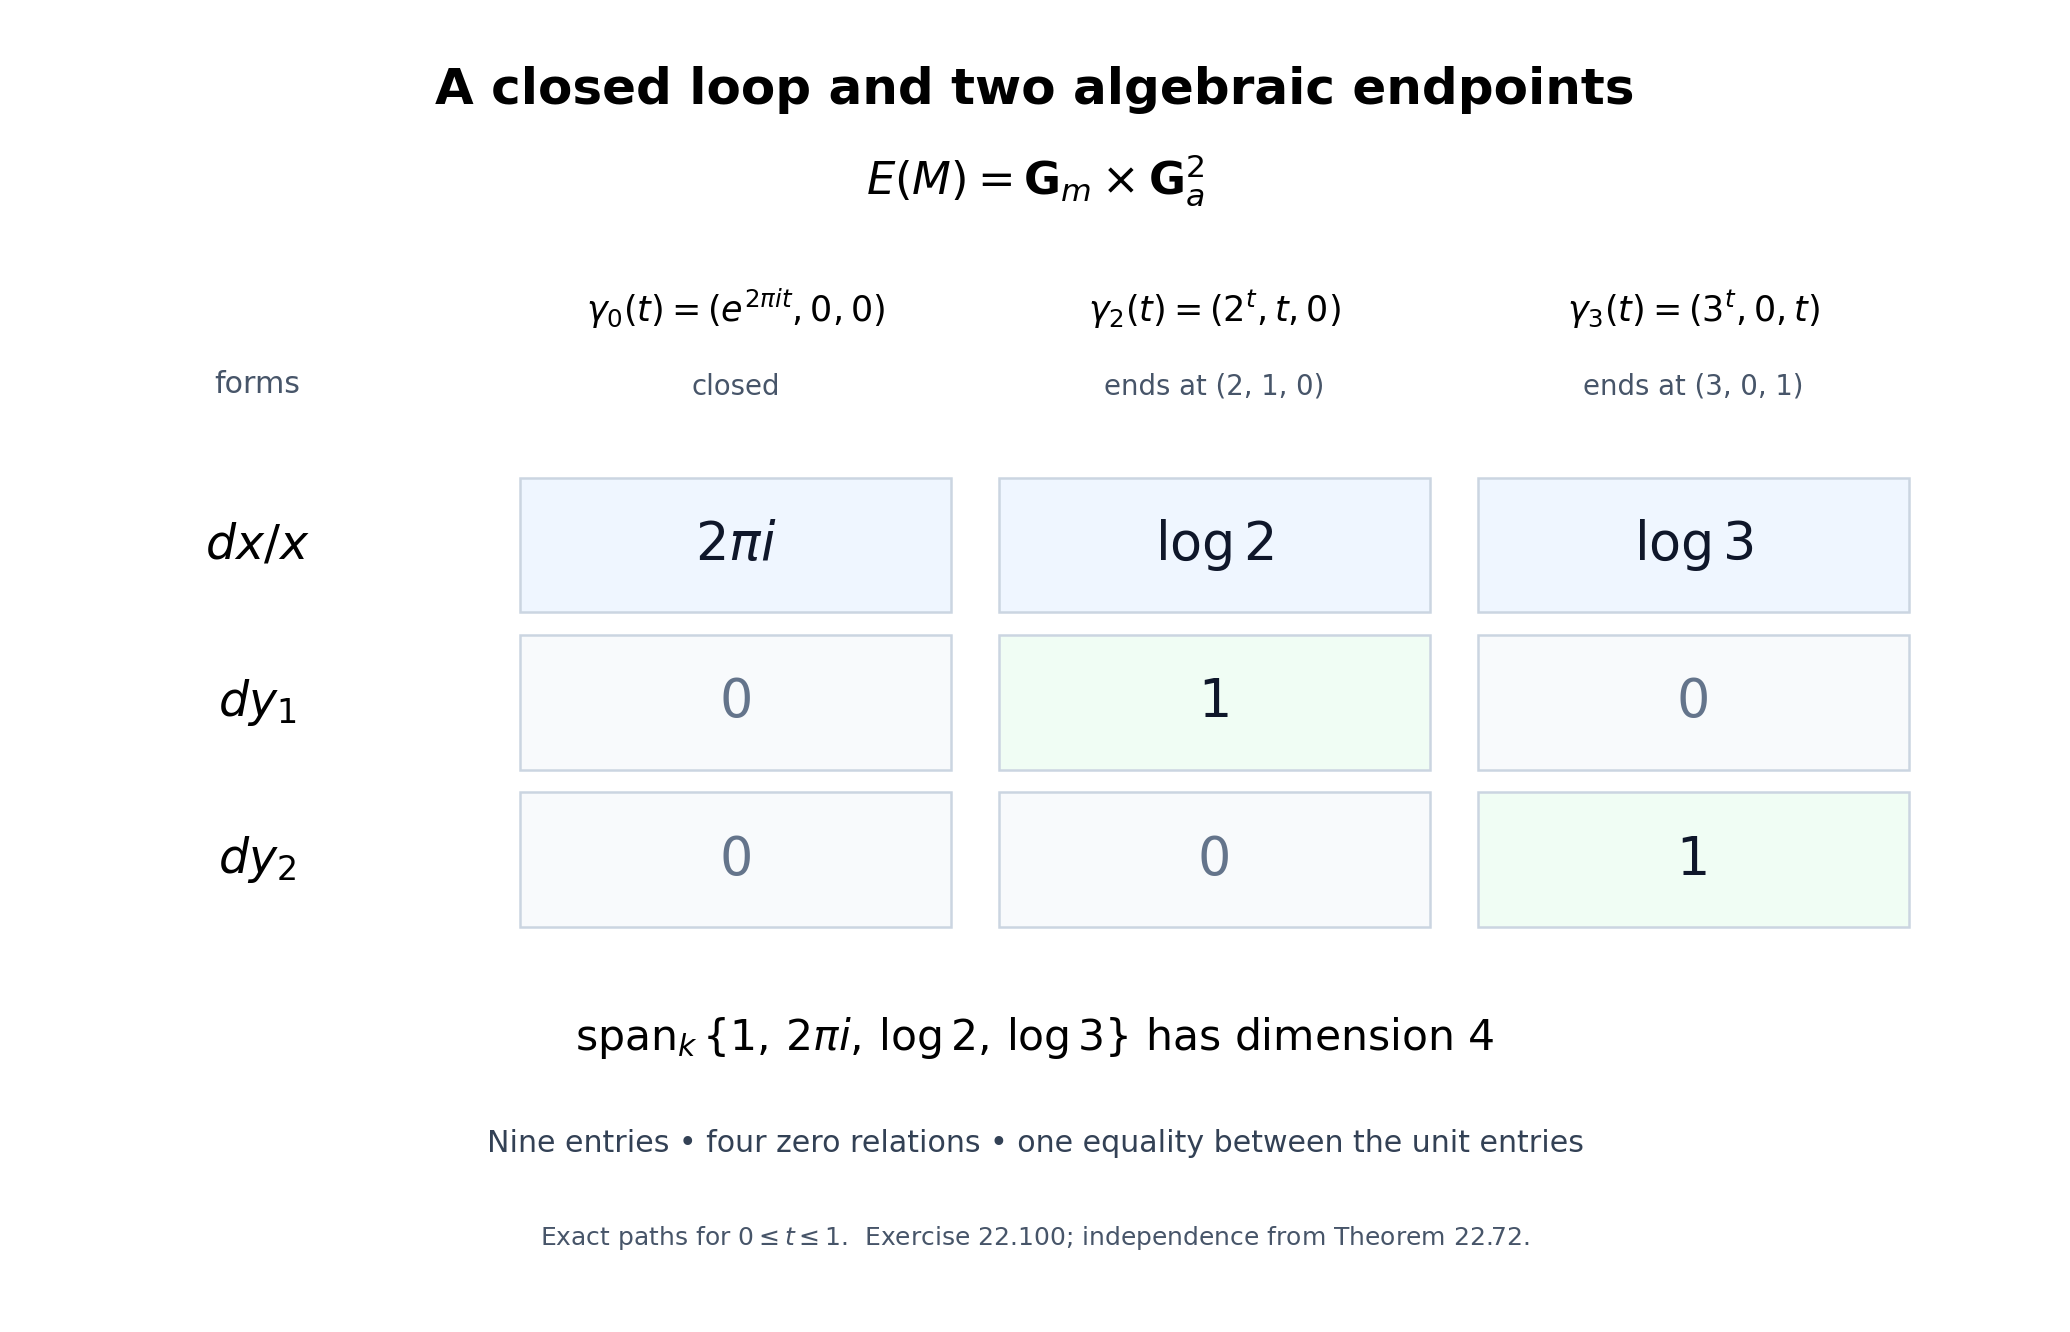
\includegraphics[keepaspectratio,alt={The exact period matrix for two multiplicative endpoints, with the closed path and two lifted endpoint paths specified.}]{../verification/lesson22/relative-period-matrix.png}}
\par\smallskip
\begin{flushleft}\small
\emph{Figure 22.7. Exercise 22.100. The columns are the exact paths
\((e^{2\pi it},0,0)\), \((2^t,t,0)\), and \((3^t,0,t)\) in
\(\mathbf G_m(\mathbf C)\times\mathbf C^2\), for \(0\le t\le1\). The
four zero entries express cross-factor pairings; the two unit entries
give one additional relation. The four remaining scalar directions are
independent by Theorem 22.72.}
\end{flushleft}
\end{minipage}\par\medskip


For the construction and relation theorem, see Annette Huber and Gisbert
Wüstholz,
\href{https://home.mathematik.uni-freiburg.de/arithgeom/preprints/huber-einsmotive.pdf}{\emph{Transcendence
and linear relations of 1-periods}}, Chapters 8--9.

\subsection{Relative curve integrals: an explicit
comparison}\label{relative-curve-integrals-an-explicit-comparison}

Let \(k=\overline{\mathbf Q}\). Consider \[
 C=\mathbf A^1_k\setminus\{a_1,\ldots,a_s\},\qquad
 D=\{b,d_1,\ldots,d_r\}\subset C(k),
\] where the punctures are distinct and the endpoints are distinct.
Either \(s\) or \(r\) may be zero. A relative one-cycle is a finite
integral combination of oriented, piecewise smooth paths in
\(C(\mathbf C)\) whose boundary is supported on \(D\). Boundaries of
two-chains and chains supported on \(D\) give the relative homology
group \(H_1(C,D;\mathbf Z)\).

\subsubsection{Lemma 22.101. Forms and endpoints in relative degree
one}\label{lemma-22.101.-forms-and-endpoints-in-relative-degree-one}

Put \(R=k[x,1/\prod_i(x-a_i)]\), with the empty product interpreted as
\(1\). The relative algebraic de Rham group is \[
 H^1_{\mathrm{dR}}(C,D)
   =\frac{R\,dx\oplus k^D}
          {\{(df,f|_D):f\in R\}}.
 \tag{22.251}
\] Its pairing with a relative cycle is \[
 \bigl\langle[\omega,\eta],[\gamma]\bigr\rangle
       =\int_\gamma\omega-\eta(\partial\gamma).
 \tag{22.252}
\] For \(1\le j\le r\), let \(q_j\in k[x]\) be the Lagrange polynomial
with value \(1\) at \(d_j\) and value \(0\) at all other points of
\(D\). A basis of (22.251) is \[
 [\xi_i,0]\quad(1\le i\le s),\qquad
 [dq_j,0]\quad(1\le j\le r),\qquad
 \xi_i=\frac{dx}{x-a_i}.
 \tag{22.253}
\]

\textbf{Proof.} The relative de Rham complex is the shifted mapping cone
of restriction from \(C\) to \(D\). In degrees zero and one its global
complex is \(R\to R\,dx\oplus k^D\), with the differential in (22.251);
there are no terms of higher degree. It computes the sheaf complex
because \(C\) and \(D\) are affine and its terms are quasi-coherent, by
the affine Čech acyclicity used in Proposition 22.84.

The fundamental theorem of calculus shows that \((df,f|_D)\) pairs to
zero. A one-form on a smooth curve is closed. Stokes' formula on each
subdivided smooth two-simplex therefore makes its integral over a
boundary zero; the endpoint term also vanishes because \(\partial^2=0\).
A path supported on the finite set \(D\) is constant. Thus (22.252) is
well defined.

Interpolate any \(\eta\in k^D\) by a polynomial \(h\). Subtracting
\((dh,h|_D)\) replaces \((\omega,\eta)\) by \((\omega-dh,0)\). Partial
fractions, integrated term by term except at simple poles, give \[
 \omega-dh=df+\sum_i c_i\xi_i,\qquad f\in R,\quad c_i\in k.
\] More explicitly, a polynomial has a polynomial primitive, and
\((x-a)^{-m}dx=d((x-a)^{1-m}/(1-m))\) for \(m\ge2\). Now put
\(g=f-f(b)-\sum_j(f(d_j)-f(b))q_j\). It vanishes on \(D\), so \((dg,0)\)
is a relative coboundary. This proves spanning by (22.253).

For independence, suppose \(\sum_i c_i\xi_i+\sum_j e_jdq_j=df\), with
\(f|_D=0\). An exact rational differential has residue zero at every
point: differentiation of its Laurent series has no coefficient of
\((x-a)^{-1}dx\). Taking residues gives \(c_i=0\) for every \(i\).
Consequently \(\sum_j e_jq_j-f\) has derivative zero and is constant.
Its value at \(b\) is zero, and its value at \(d_j\) is \(e_j\). Hence
every \(e_j=0\). \(\square\)

\subsubsection{Theorem 22.102. The relative curve pairing is a 1-motive
pairing}\label{theorem-22.102.-the-relative-curve-pairing-is-a-1-motive-pairing}

Define \[
 M_{C,D}=[\mathbf Z^r\xrightarrow{u}\mathbf G_m^s],
 \qquad
 u(e_j)_i=\frac{d_j-a_i}{b-a_i}.
 \tag{22.254}
\] There are isomorphisms \[
 H_1(C,D;\mathbf Z)\simeq T_B(M_{C,D}),\qquad
 H^1_{\mathrm{dR}}(C,D)\simeq V_{\mathrm{dR}}(M_{C,D})^\vee
\] under which (22.252) is exactly the period pairing (22.238).

\textbf{Proof.} The universal extension from Theorem 22.92 is
\(E(M_{C,D})=\mathbf G_m^s\times\mathbf G_a^r\). There is an explicit
algebraic map \[
 \Phi:C\longrightarrow E(M_{C,D}),\qquad
 x\longmapsto
 \left(\left(\frac{x-a_i}{b-a_i}\right)_{i=1}^s,
                  (q_j(x))_{j=1}^r\right).
 \tag{22.255}
\] It sends \(b\) to the identity and \(d_j\) to \(\widetilde u(e_j)\).
If \(X_i,Y_j\) denote the multiplicative and additive coordinates, then
\(\Phi^*(dX_i/X_i)=\xi_i\) and \(\Phi^*(dY_j)=dq_j\). Lemma 22.101
therefore gives the asserted de Rham isomorphism.

Here is the integral homology calculation. A punctured plane has the
homotopy type of a graph with one circle around each puncture. One can
see this by choosing disjoint small closed discs about the punctures
inside a large disc, retracting the punctured small discs to their
boundary circles and the exterior of the large disc to its boundary.
Join the small boundary circles by disjoint arcs forming a tree, and
join that tree to the large boundary. Cutting along these arcs leaves a
disc. Triangulate that disc and collapse it toward the arcs and the
small boundary circles, leaving a graph with exactly \(s\) independent
circles. The resulting loops \(\lambda_i\), based at \(b\) by paths,
form a basis of \(H_1(C;\mathbf Z)\). The case \(s=0\) is the
contractible plane.

Choose paths \(\rho_j\) from \(b\) to \(d_j\). Every relative cycle has
a unique boundary \(\sum_jm_j(d_j-b)\). Subtracting \(\sum_jm_j\rho_j\)
gives an absolute cycle. The exact sequence of the relative chain
complex makes \(H_1(C)\to H_1(C,D)\) injective, since \(H_1(D)=0\). Thus
the \(\lambda_i\)'s and \(\rho_j\)'s form a basis of
\(H_1(C,D;\mathbf Z)\).

For a relative cycle \(\gamma\) with that boundary, set
\(z_i=\int_\gamma\xi_i\) and \(\ell=\sum_jm_je_j\). Continuation of the
elementary logarithm along each path gives \[
 \exp(z_i)=\prod_j
       \left(\frac{d_j-a_i}{b-a_i}\right)^{m_j}=u(\ell)_i.
 \tag{22.256}
\] When intermediate endpoints are not in \(D\), their factors cancel in
the product, since their coefficients in \(\partial\gamma\) are zero.
Hence \((\ell,z)\in T_B(M_{C,D})\). Its canonical lift to the Lie
algebra of \(E(M_{C,D})\) is \((z,m)\), because the additive integrals
are \(\int_\gamma dq_j=q_j(\partial\gamma)=m_j\).

On \(\lambda_i\) this construction gives the period \(2\pi i\) in the
\(i\)-th torus coordinate and zero elsewhere. Indeed the integral around
its small circle is \(2\pi i\); the other forms have primitives on that
disc, and the two traversals of each joining path cancel. On \(\rho_j\)
it gives a lift of the lattice basis vector \(e_j\). These vectors form
a basis of \(T_B(M_{C,D})\), by (22.235). This proves the integral Betti
isomorphism. Equality of the pairings follows on each basis form from
the computed integrals, hence on every class by Lemma 22.101.

For clarity, the matrix of the comparison is \[
 \begin{pmatrix}
    2\pi i\,I_s & L\\
    0&I_r
 \end{pmatrix},
 \qquad
 L_{ij}=\int_{\rho_j}\frac{dx}{x-a_i}.
 \tag{22.257}
\] Its determinant is \((2\pi i)^s\ne0\), including the empty-block
cases. This also verifies directly that the comparison becomes an
isomorphism over \(\mathbf C\). \(\square\)

For \(C=\mathbf G_m\) and \(D=\{1,2,3\}\), the interpolation polynomials
are \[
 q_1=(x-1)(3-x),\qquad q_2=\frac{(x-1)(x-2)}2.
\] Formula (22.255) is \(\Phi(x)=(x,q_1(x),q_2(x))\), and (22.257) is
exactly the matrix in Exercise 22.100. Its curved lifts of paths in
\(C\) have the same invariant-form integrals as the exponential paths
displayed in Figure 22.7, since their torus coordinates and additive
endpoint differences agree.

\subsubsection{Corollary 22.103. All relative period relations for
punctured rational
curves}\label{corollary-22.103.-all-relative-period-relations-for-punctured-rational-curves}

Every \(k\)-linear relation between the periods of \((C,D)\) follows
from bilinearity and morphisms between subquotients of finite sums of
\(M_{C,D}\). For finitely many such pairs one uses their direct sum.

\textbf{Proof.} Theorem 22.102 identifies each entire pairing, including
its rational and algebraic vector spaces, with a 1-motive pairing.
Theorem 22.98 applies to these identified symbols. It gives the stated
generators and the specified category of subquotients. \(\square\)

This statement describes relations through 1-motives. It does not
identify those generators with a smaller list consisting only of maps
between curves.

\subsubsection{Theorem 22.104. Algebraicity of a rational differential
integral}\label{theorem-22.104.-algebraicity-of-a-rational-differential-integral}

Let \(\omega=R(x)\,dx\), with \(R\in k(x)\), and let \(\gamma\) be a
finite integral combination of paths in the complex affine line avoiding
its poles and having boundary supported on finitely many algebraic
points. Write the partial-fraction decomposition in the form \[
 \omega=dF+\sum_{i=1}^s c_i\frac{dx}{x-a_i},
 \qquad
 F\in k(x),\quad c_i=\operatorname{res}_{a_i}\omega,
 \tag{22.258}
\] where \(a_i\) includes all finite poles. Then \[
 \int_\gamma\omega\in k
 \quad\Longleftrightarrow\quad
 \sum_i c_i\int_\gamma\frac{dx}{x-a_i}=0.
 \tag{22.259}
\] When these conditions hold, the integral is \(F(\partial\gamma)\). In
particular, a nonzero integral over a closed cycle is transcendental.

\textbf{Proof.} Partial fractions give (22.258) by the explicit
integration used in Lemma 22.101. The primitive \(F\) has no finite
poles outside the poles of \(\omega\), so it is defined at the boundary
points. Its endpoint contribution \(F(\partial\gamma)\) lies in \(k\);
nonalgebraic intermediate endpoints cancel.

Put \(z_i=\int_\gamma dx/(x-a_i)\). Formula (22.256), or the same
cancellation argument without a selected base point, proves
\(e^{z_i}\in k^*\). Select a rational basis \(v_1,\ldots,v_m\) of the
span of the \(z_i\)'s. Each \(v_j\) can be selected from the \(z_i\)'s
themselves, so it is a logarithm of an algebraic number. Theorem 22.72
says that \(1,v_1,\ldots,v_m\) are linearly independent over \(k\).
Therefore the \(k\)-linear combination \(\sum_i c_iz_i\) is algebraic
only when it is zero. The same conclusion is immediate if \(m=0\).
Combining this with (22.258) proves (22.259).

If \(\partial\gamma=0\), the exact-form contribution vanishes. The
integral is then either zero or transcendental. \(\square\)

The condition depends on the chosen paths: changing a path by a loop
changes its logarithms by integral multiples of \(2\pi i\). Both the
formula and the criterion retain those multiples.

\subsubsection{Exercise 22.105. A rational integral of the third
kind}\label{exercise-22.105.-a-rational-integral-of-the-third-kind}

Compute \[
 I=\int_0^1\frac{dx}{1+x^3}
 \tag{22.260}
\] and prove that it is transcendental.

\textbf{Solution.} Partial fractions give \[
 \frac1{1+x^3}
   =\frac1{3(x+1)}
      +\frac{2-x}{3(x^2-x+1)}.
 \tag{22.261}
\] An antiderivative on the real interval is \[
 \frac13\log(x+1)-\frac16\log(x^2-x+1)
       +\frac1{\sqrt3}
          \arctan\left(\frac{2x-1}{\sqrt3}\right).
 \tag{22.262}
\] The two arctangent values at the endpoints are \(\pi/6\) and
\(-\pi/6\); the quadratic has value \(1\) at both endpoints.
Consequently \[
 I=\frac{\log2}{3}+\frac{\pi}{3\sqrt3}.
 \tag{22.263}
\] The rational differential has only simple finite poles and no
polynomial part, so its primitive \(F\) in (22.258) can be taken to be
zero. Its integral is positive, because the integrand is positive on
\([0,1]\). Theorem 22.104 therefore makes \(I\) transcendental.
Equivalently, its displayed value is a nonzero algebraic linear
combination of \(\log2\) and the logarithm \(i\pi\) of \(-1\), to which
Theorem 22.72 applies.

The relative pairing and its comparison with 1-motives are discussed in
Huber and Wüstholz,
\href{https://home.mathematik.uni-freiburg.de/arithgeom/preprints/huber-einsmotive.pdf}{\emph{Transcendence
and linear relations of 1-periods}}, Sections 12.2--12.3. Their Section
13.2 discusses rational differential integrals, including (22.260).

\subsection{Jacobians and the periods of a
curve}\label{jacobians-and-the-periods-of-a-curve}

Let \(\overline C\) be a smooth projective connected curve over
\(k=\overline{\mathbf Q}\), let \(S\subset\overline C(k)\) be finite,
and put \(U=\overline C\setminus S\). Fix \(b\in U(k)\). Write
\(g=\dim H^1(\overline C,\mathcal O_{\overline C})\).

We use the scheme-theoretic construction in
\href{../AG-HP/the-picard-functor-and-the-picard-scheme-of-a-curve.html\#7-degree-pieces-abel-fibres-and-properness}{\emph{The
Picard functor and the Picard scheme of a curve}, Theorem 2.1 and
Sections 5--7}. It supplies the Jacobian
\(J=\operatorname{Pic}^0(\overline C)\), its universal line bundle
\(\mathcal P\) normalized along \(b\times J\), and the projective-bundle
description of the Abel map in degree \(n>2g-2\). These are functorial
statements about line bundles, including families.

\subsubsection{Proposition 22.106. The Abel map identifies rational
first
homology}\label{proposition-22.106.-the-abel-map-identifies-rational-first-homology}

The map \[
 \iota:\overline C\longrightarrow J,\qquad
       x\longmapsto[\mathcal O_{\overline C}(x-b)]
 \tag{22.264}
\] induces an isomorphism
\(H_1(\overline C;\mathbf Q)\simeq H_1(J;\mathbf Q)\).

\textbf{Proof.} We first compute the first cohomology of a symmetric
power. Triangulate the compact surface \(\overline C(\mathbf C)\). The
product cell decomposition on its \(n\)-fold product is preserved by
permutations. Barycentric subdivision makes every element stabilizing a
simplex fix that simplex pointwise: a simplex is a chain of product
faces, whose distinct dimensions force every face in the chain to be
fixed.

Thus the quotient has cells given by the simplex orbits, with the same
face identifications. Pullback identifies its cellular cochains with the
permutation-invariant cochains of the product. Taking invariants over
\(\mathbf Q\) commutes with cohomology. Indeed averaging over the finite
group commutes with the differential; an invariant coboundary has an
invariant primitive obtained by averaging, and an invariant cohomology
class has an invariant representative by the same operation.
Consequently \[
 H^1(\operatorname{Sym}^n\overline C;\mathbf Q)
    \simeq H^1(\overline C^n;\mathbf Q)^{\mathfrak S_n}
    \simeq H^1(\overline C;\mathbf Q).
 \tag{22.265}
\] For the last step, degree-one product cohomology is the direct sum of
the pullbacks from the factors. This follows directly from the cellular
product complex: in total degree one exactly one factor has degree one
and the other factors have degree zero; connectedness leaves one copy of
\(\mathbf Q\) in each degree-zero cohomology group. Permutation
invariants are therefore the diagonal tuples \((\alpha,\ldots,\alpha)\).
In particular, pullback by \(j(x)=x+(n-1)b\) is the isomorphism in
(22.265), with no factor of \(n\).

Choose \(n\ge\max(2,2g-1)\). The cited Picard construction proves that
\[
 a_n:\operatorname{Sym}^n\overline C\longrightarrow J,\qquad
              D\longmapsto[\mathcal O(D-nb)]
 \tag{22.266}
\] is a projective bundle with fibre \(\mathbf P^{n-g}\). Its analytic
map is locally a product. A connected, simply connected fibre makes the
induced fundamental-group map an isomorphism: lift a loop through
successive product charts and join its two endpoint lifts inside the
fibre; a null-homotopy lifts after subdivision into such charts, and any
resulting fibre loop contracts. Complex projective space is simply
connected, as its cell decomposition has one zero-cell and only cells of
positive even dimension; its one-skeleton is a point. A point fibre
satisfies the same assertion. Abelianizing the fundamental groups gives
the first-homology isomorphism for \(a_n\), hence also the
first-cohomology isomorphism.

Since \(a_nj=\iota\), (22.265) now makes \(\iota^*\) an isomorphism.
Dualizing finite-dimensional rational homology and cohomology proves the
assertion. This proof includes \(g=0\), when both first homology groups
are zero. \(\square\)

\subsubsection{Lemma 22.107. De Rham comparison in the three geometries
used
here}\label{lemma-22.107.-de-rham-comparison-in-the-three-geometries-used-here}

Integration gives a natural isomorphism \[
 H^m_{\mathrm{dR}}(X/k)\otimes_k\mathbf C
       \simeq H^m(X(\mathbf C);\mathbf C)
 \tag{22.267}
\] in each of the following cases:

\begin{enumerate}
\def\labelenumi{\arabic{enumi}.}
\tightlist
\item
  \(X\) is smooth projective;
\item
  \(X\) is a smooth projective curve with finitely many points removed;
\item
  \(X\) is a torsor under a split torus over a smooth projective
  variety.
\end{enumerate}

In particular the pairing in degree one is ordinary integration of
forms, with the Čech endpoint terms when a class needs more than one
chart.

\textbf{Proof.} For a smooth projective \(X\), the cohomological GAGA
theorem used in Theorem 22.94 applies to every coherent sheaf
\(\Omega_X^p\). The spectral sequences of the algebraic and analytic de
Rham complexes therefore agree after complexification. The analytic de
Rham complex resolves the constant sheaf: on a coordinate polydisc,
integration along radial segments gives the Poincaré homotopy for closed
holomorphic forms. More explicitly, contraction with the radial vector
field, integrated after the dilation \(z\mapsto tz\), satisfies
\(dh+hd=1-\operatorname{ev}_0\). It is holomorphic by integration of
convergent power series on smaller polydiscs.

The cohomology of the constant sheaf on a manifold is singular
cohomology. This identification can be obtained from a good cover: its
finite intersections contract to points, the singular cochain complexes
on them have only degree-zero cohomology, and the Čech double complex
reduces to the nerve complex of constants. Subdivision makes singular
chains subordinate to this cover, so the same double complex computes
singular cohomology. These comparisons send a local primitive difference
to its integral along the intervening path. Thus they give integration,
with the sign convention of (22.252) and the Čech formula of Proposition
22.86.

For a curve \(\overline X\) with punctures \(S\), use the coherent
logarithmic complex \[
 \mathcal O_{\overline X}\longrightarrow
               \Omega^1_{\overline X}(S).
 \tag{22.268}
\] It has the same algebraic hypercohomology as the de Rham complex on
\(X=\overline X\setminus S\). To verify this locally at a puncture,
choose a uniformizer \(t\). A rational function with a pole has a finite
principal part \(\sum_{j<0}c_jt^j\). Differentiation maps these
principal parts bijectively onto the polar parts of differentials of
order at least two, since \(d(t^j)=jt^{j-1}dt\) and the characteristic
is zero. Hence the quotient of the meromorphic de Rham complex by
(22.268) is acyclic. The open immersion is affine on these charts, so
its direct image has no higher quasi-coherent cohomology on affine
charts. This proves the asserted hypercohomology identification.

Analytically the logarithmic complex on a disc has one constant class in
degree zero and the class \(dt/t\) in degree one at the puncture. A
convergent power series integrates termwise except for that logarithmic
term. On the punctured disc, Laurent series give the same calculation;
dividing nonzero integer exponents does not destroy normal convergence
on compact annuli. Integration of \(dt/t\) around a positive circle is
\(2\pi i\). Thus this local comparison agrees with the cohomology of the
punctured disc and its restriction maps. It identifies the analytic
logarithmic complex with the derived direct image of the constant sheaf
on \(X\). GAGA applied to the two coherent terms of (22.268) finishes
the curve case.

For a torsor \(X\to B\) under \(\mathbf G_m^t\), the \(t\) coordinate
characters give line bundles \(N_1,\ldots,N_t\) on \(B\), and \[
 X=N_1^\times\times_B\cdots\times_BN_t^\times
 \ \subset\
 \overline X=\prod_B\mathbf P(\mathcal O_B\oplus N_i).
 \tag{22.269}
\] Here \(N_i^\times\) is the complement of the zero section. This
description follows by gluing the multiplicative transition functions of
the torsor. The compactification is smooth projective, with boundary the
coordinate zero and infinity sections. On a bundle chart its logarithmic
forms are base forms and \(dt_i/t_i\).

The algebraic logarithmic complex on this chart includes into the
complex with Laurent-polynomial fibre coefficients. Its quotient is a
sum of weights \(m=(m_1,\ldots,m_t)\) with at least one negative
coordinate. On such a weight choose \(m_j\ne0\). Cartan's identity gives
\[
 d\bigl(m_j^{-1}\iota_{t_j\partial/\partial t_j}\bigr)
 +\bigl(m_j^{-1}\iota_{t_j\partial/\partial t_j}\bigr)d=1.
 \tag{22.270}
\] This contraction includes base forms, whose fibre weight is zero. It
makes the quotient acyclic. The assertion is local, so the contractions
need not agree on overlaps. The open immersion is affine on the bundle
charts, giving the algebraic hypercohomology comparison as above.

On analytic charts the same power-series argument removes all nonzero
weights and the ordinary coordinate directions. The remaining classes
are the exterior products of the logarithmic forms at those boundary
components passing through the point. Small punctured polydiscs retract
to products of circles; integration sends those exterior products to
their cohomology bases, with factor \(2\pi i\) for each circle. Thus the
analytic logarithmic complex computes the derived direct image of the
constant sheaf from \(X\). Applying GAGA termwise to the coherent
logarithmic complex on \(\overline X\) proves (22.267). All inclusions,
pullbacks and integration maps used in this construction are natural.
\(\square\)

\subsubsection{Proposition 22.108. A generalized Jacobian from framed
line
bundles}\label{proposition-22.108.-a-generalized-jacobian-from-framed-line-bundles}

There are a semiabelian variety \(G=J(U)\) and a map \(a:U\to G\), with
\(a(b)=0\), fitting into \[
 0\longrightarrow T\longrightarrow G\longrightarrow J\longrightarrow0,
 \qquad
 T=\mathbf G_m^S/\mathbf G_m,\quad
 \dim T=|S|-1
 \tag{22.271}
\] when \(S\ne\varnothing\). If \(S=\varnothing\), take \(G=J\),
\(T=0\), and \(a=\iota\). The composite \(U\to G\to J\) is the
restriction of (22.264).

\textbf{Proof.} Suppose \(S\ne\varnothing\). Over a degree-zero line
bundle \(L\) on \(\overline C\), take a nonzero vector \(v_s\in L_s\)
for each \(s\in S\), modulo simultaneous scalar multiplication. More
generally these are relative framings over a test scheme, with
isomorphisms of bundles carrying all the vectors to the specified
vectors. This functor is represented over \(J\) by \[
 G=\left(\prod_{s\in S}\mathcal P_s^\times\right)/\mathbf G_m.
 \tag{22.272}
\] To see the quotient without assuming a general quotient construction,
fix \(s_0\in S\). It is the fibre product of the frame bundles of
\(N_s=\mathcal P_s\otimes\mathcal P_{s_0}^{-1}\), for \(s\ne s_0\); send
the frame tuple to \(v_s\otimes v_{s_0}^{-1}\). Conversely locally
choose \(v_{s_0}\), recover the other vectors from those ratios, and
note that another choice changes all vectors by the same unit. This
proves the description on every test scheme by descent. In particular
\(G\to J\) is a Zariski locally trivial torus torsor.

Tensor product of framed line bundles defines multiplication; the
trivial line bundle with its constant frames is the identity, and
dualizing gives the inverse. These are algebraic morphisms. Indeed the
universal normalized bundle identifies the line bundle at a sum in \(J\)
with the tensor product of the two bundles, uniquely after normalization
at \(b\). Uniqueness is the scalar-removal assertion of the cited Picard
Theorem 2.1, so these identifications satisfy associativity on all test
schemes. The construction is commutative. Its kernel over \(0\in J\) is
exactly the quotient torus in (22.271). Local products with this torus
show that \(G\) is smooth and connected. Thus (22.271) makes \(G\)
semiabelian.

The family of divisors \(x-b\), parametrized by \(x\in U\), avoids
\(S\). The canonical section \(1\) of \(\mathcal O(x-b)\) therefore
gives a nonzero vector in each fibre over \(S\). It defines the required
morphism \(a\) by (22.272). At \(x=b\) the divisor is zero and all
frames are \(1\), so \(a(b)=0\). \(\square\)

\subsubsection{Theorem 22.109. The open-curve homology
comparison}\label{theorem-22.109.-the-open-curve-homology-comparison}

The map \(a\) induces an isomorphism \[
 a_*:H_1(U;\mathbf Q)\xrightarrow{\sim}H_1(G;\mathbf Q),
 \qquad
 a^*:H^1_{\mathrm{dR}}(G)\xrightarrow{\sim}H^1_{\mathrm{dR}}(U),
 \tag{22.273}
\] compatible with integration.

\textbf{Proof.} The case \(S=\varnothing\) follows from Proposition
22.106 and the projective comparison of Lemma 22.107. Suppose
\(S\ne\varnothing\). The topological exact sequence for the punctures is
\[
 0\longrightarrow
   \mathbf Q^S/\mathbf Q(1,\ldots,1)
 \longrightarrow H_1(U;\mathbf Q)
 \longrightarrow H_1(\overline C;\mathbf Q)\longrightarrow0.
 \tag{22.274}
\] For completeness, excision identifies the degree-two relative group
of \((\overline C,U)\) with one copy of \(\mathbf Q\) for each small
puncture disc, and its degree-one relative group is zero. An oriented
fundamental cycle of the compact connected surface maps to
\((1,\ldots,1)\). One can check that its degree-two homology is
precisely \(\mathbf Q\) on a triangulation: the boundary equation makes
the coefficients of adjacent oriented triangles equal, and all triangles
are connected by adjacency. The relative long exact sequence now gives
(22.274). Its left-hand generators are the positively oriented puncture
loops.

For (22.271), the period-lattice argument of Theorem 22.94 gives \[
 0\longrightarrow H_1(T;\mathbf Q)
 \longrightarrow H_1(G;\mathbf Q)
 \longrightarrow H_1(J;\mathbf Q)\longrightarrow0.
 \tag{22.275}
\] Use \(s_0\) as reference in (22.272). The map on the left of these
sequences sends the loop at \(s\ne s_0\) to the \(s\)-th coordinate
circle of \(T\), and the loop at \(s_0\) to minus the sum of all those
circles. Here is the local calculation fixing the signs. Near \(s\),
take a coordinate \(y\) on the curve and let \(t\) be the moving-point
coordinate, with \(s\) given by \(y=0\). The bundle
\(\mathcal O(\Delta)\) has generator \((y-t)^{-1}\), so its canonical
section \(1\), restricted to \(y=0\), has coefficient \(-t\). Its frame
therefore winds once positively when \(t\) winds positively. The factor
\(\mathcal O(-b)\) is nonvanishing there. Other puncture frames are
nonvanishing across this disc. Taking the ratio to the reference frame
gives exactly the asserted coordinate windings. At \(s_0\) the common
denominator winds once, giving every ratio winding \(-1\).

This is the isomorphism
\(\mathbf Q^S/\mathbf Q(1,\ldots,1)\simeq H_1(T;\mathbf Q)\). The right
map is the isomorphism of Proposition 22.106. The two exact sequences
commute with \(a\) and \(\iota\), so a direct diagram chase proves that
the middle map is an isomorphism.

Both \(U\) and \(G\) are among the cases of Lemma 22.107. Its naturality
makes the complexification of \(a^*\) the dual of the homology map just
proved. Extension of a field is faithful, so \(a^*\) itself is an
isomorphism over \(k\). The same comparison proves compatibility with
integration. \(\square\)

\subsubsection{Proposition 22.110. Universal-extension forms represent
semiabelian
cohomology}\label{proposition-22.110.-universal-extension-forms-represent-semiabelian-cohomology}

For a semiabelian variety \(G\), invariant forms give an isomorphism \[
 \operatorname{Lie}(G^\natural)^\vee
       \xrightarrow{\sim} H^1_{\mathrm{dR}}(G).
 \tag{22.276}
\] If a loop in \(G\) corresponds to \(\lambda\in\Lambda_G\), its
integral against this class is evaluation of the covector on the unique
period lift of \(\lambda\) to \(\operatorname{Lie}G^\natural\).

\textbf{Proof.} Pullback along the vector torsor \(G^\natural\to G\) is
an isomorphism on de Rham cohomology by Proposition 22.84. Invariant
forms on \(G^\natural\) are closed, because the group is commutative.
The argument of Theorem 22.85 proves injectivity into cohomology: if
such a form is globally exact, its primitive, minus its value at the
identity, is an additive algebraic homomorphism to \(\mathbf G_a\).
Proposition 22.91 makes that homomorphism zero.

Write \(\dim A=g\) and \(\dim T=t\). The source has dimension \(2g+t\).
By Lemma 22.107 and the exact period lattices in Theorem 22.94, the
target also has dimension \(\operatorname{rank}\Lambda_G=2g+t\). Thus
the injection is an isomorphism. The integral identity follows by
lifting the loop through the vector torsor and then through the
exponential cover, exactly as in Proposition 22.86. Vector fibres add no
periods. \(\square\)

\subsubsection{Theorem 22.111. The full relative curve
pairing}\label{theorem-22.111.-the-full-relative-curve-pairing}

Let \(D=\{b,d_1,\ldots,d_r\}\subset U(k)\) be a finite nonempty set.
Define \[
 M(U,D)=
 \left[\mathbf Z[D]^0\longrightarrow G\right],
 \qquad d_j-b\longmapsto a(d_j),
 \tag{22.277}
\] where \(\mathbf Z[D]^0\) is the group of degree-zero divisors
supported on \(D\). Then there are isomorphisms \[
 H_1(U,D;\mathbf Q)\simeq V_B(M(U,D)),\qquad
 H^1_{\mathrm{dR}}(U,D)\simeq V_{\mathrm{dR}}(M(U,D))^\vee
 \tag{22.278}
\] identifying the integration pairing with the 1-motive period pairing.

\textbf{Proof.} Put \(M=M(U,D)\) and \(E=E(M)\). Pull back its vector
extension along \(a\): \[
 X=U\times_G E,\qquad \pi:X\to U,\qquad f:X\to E.
 \tag{22.279}
\] Choose the finite subset \(D'\subset X(k)\) consisting of \((b,0)\)
and \((d_j,\widetilde u(d_j-b))\). These are distinct points. The
construction does not require the points \(a(d_j)\) in \(G\) to be
distinct.

The map of pairs \((X,D')\to(U,D)\) induces isomorphisms on both
cohomology and homology. Algebraically, vector-torsor invariance,
Proposition 22.84, gives the absolute de Rham assertion; the map
\(D'\to D\) is an isomorphism, so the relative long exact sequences give
the relative assertion. Topologically, this vector torsor has a
continuous section: combine local sections by a partition of unity using
affine combinations in each fibre. Correct the section near the finitely
many points of \(D\), using disjoint local bump functions, so that it
passes through \(D'\). Linear contraction in the vector fibres then
gives a deformation to that section fixing \(D'\). This proves the
homology assertion.

For a relative cycle in \(X\) with boundary
\(\sum_jm_j((d_j,\widetilde u(d_j-b))-(b,0))\), integrate the invariant
forms of \(E\) after applying \(f\). Their values define a vector
\(w\in\operatorname{Lie}E(\mathbf C)\). Lifting paths through the
exponential cover gives \[
 \exp_E(w)=\sum_jm_j\widetilde u(d_j-b)
           =\widetilde u\!\left(\sum_jm_j(d_j-b)\right).
 \tag{22.280}
\] This also holds when the chain's individual endpoints are not in
\(D'\): their contributions cancel in its boundary. Thus \(w\) is the
canonical lift of a Betti vector of \(M\), by Theorem 22.94. Homologous
cycles give the same vector, since invariant forms are closed. We obtain
the first map in (22.278).

Compare the exact sequences with absolute groups on the left and
endpoint lattices on the right. The absolute map is the isomorphism
\(H_1(U;\mathbf Q)\to H_1(G;\mathbf Q)\) from Theorem 22.109, followed
by the unique period lift. The endpoint map is the identity on
\(\mathbf Q[D]^0\). Exactness of (22.235) and the relative homology
sequence proves that the middle map is an isomorphism.

For de Rham cohomology, send an invariant covector \(\omega\) on \(E\)
to the class \([f^*\omega,0]\) in \(H^1_{\mathrm{dR}}(X,D')\), and then
use \(\pi^*\) to identify this with \(H^1_{\mathrm{dR}}(U,D)\). The
relevant exact sequences are \[
 \begin{array}{ccccccccc}
 0&\to&(\mathbf Z[D]^0\otimes k)^\vee
 &\to&\operatorname{Lie}E^\vee
 &\to&\operatorname{Lie}G^\natural{}^\vee&\to&0\\
 &&\downarrow&&\downarrow&&\downarrow\\
 0&\to&k^D/k
 &\to&H^1_{\mathrm{dR}}(U,D)
 &\to&H^1_{\mathrm{dR}}(U)&\to&0 .
 \end{array}
 \tag{22.281}
\] The right vertical map is (22.276) followed by (22.273). To verify
it, use any product description
\(E=G^\natural\times(\mathbf Z[D]^0\otimes k)\); additive-coordinate
differentials are exact in absolute cohomology, so the absolute class of
\(\omega\) is that of its restriction to \(G^\natural\).

On the left, a functional \(c\) on the lattice vector space gives the
additive function \(F_c:E\to\mathbf G_a\). At the selected points it has
values \(0,c(d_1-b),\ldots,c(d_r-b)\). The relative class
\([d(f^*F_c),0]\) is \([0,-F_c|_{D'}]\), by (22.251). Hence the left
vertical map sends \(c\) to the class of the endpoint function with
values \(0,-c(d_1-b),\ldots,-c(d_r-b)\). This is an isomorphism and
fixes the sign in the diagram. Exactness now proves that the middle
vertical map is an isomorphism.

Finally, the two constructions use exactly the same invariant-form
integrals on \(X\). Their pairings are equal by definition, proving
(22.278) with the asserted compatibility. \(\square\)

If no endpoint set is specified, choose a single base point \(D=\{b\}\).
The relative groups then equal the absolute degree-one groups and the
lattice in (22.277) is zero. For a disconnected smooth curve, apply the
construction component by component and take the direct sum.

It follows from Theorems 22.98 and 22.111 that every linear relation
among periods of a fixed smooth curve relative to algebraic endpoints is
generated by bilinearity and morphisms between subquotients of finite
sums of its 1-motive (22.277). This includes differential forms of the
first, second and third kinds. The claim concerns these 1-motive
morphisms; converting every generator to maps between curves alone is a
further statement.

\subsubsection{Exercise 22.112. A punctured elliptic curve with relative
endpoints}\label{exercise-22.112.-a-punctured-elliptic-curve-with-relative-endpoints}

Let \[
 E:\ y^2=4x^3-g_2x-g_3
\] be nonsingular over \(k\), with origin \(O\). Choose
\(Q=(a,b_Q)\in E(k)\) with \(b_Q\ne0\), and let \(U=E\setminus\{O,Q\}\).
Choose \(P_0,P_1\in U(k)\) with distinct \(x\)-coordinates \(x_0,x_1\).
Give a de Rham basis for \((U,\{P_0,P_1\})\), a compatible period-matrix
shape, and the dimensions of its two realizations.

\textbf{Solution.} The generalized Jacobian is an extension of \(E\) by
one copy of \(\mathbf G_m\). The endpoint lattice has rank one.
Consequently the de Rham dimension and Betti rank of the relative motive
are both \(2+1+1=4\).

Put \[
 \alpha=\frac{dx}{y},\qquad
 \beta=\frac{x\,dx}{y},\qquad
 \rho=\frac{y+b_Q}{2(x-a)y}\,dx,\qquad
 F=\frac{x-x_0}{x_1-x_0}.
 \tag{22.282}
\] The form \(\rho\) has residue \(1\) at \(Q\) and residue \(-1\) at
\(O\), with no other poles. At \(Q\), use \(x-a\) as a uniformizer: the
numerator tends to \(2b_Q\). At \(-Q\), the numerator vanishes,
cancelling \(x-a\). At other finite branch points \(dx/y\) is regular
and \(x-a\ne0\). At \(O\), the uniformizer \(t=-2x/y\) of Proposition
22.88 gives \(x=t^{-2}+O(t^2)\); hence \(\rho=-dt/t+\) regular terms.
These calculations prove all the residue assertions.

The classes of \(\alpha,\beta\) form the complete-curve de Rham basis
from Proposition 22.88. They remain independent on \(U\). Indeed the
quotient of the logarithmic complex for the punctures by the regular de
Rham complex is concentrated in degree one, so its hypercohomology
sequence injects \(H^1_{\mathrm{dR}}(E)\) into \(H^1_{\mathrm{dR}}(U)\).
The local principal-part argument in Lemma 22.107 identifies this
injection with restriction of the two classes, including the second-kind
representative \(\beta\). The nonzero residue of \(\rho\) adds the third
independent direction. The dimension is three by Theorem 22.109. Finally
\(F(P_0)=0\), \(F(P_1)=1\); therefore \([dF,0]\) adds the independent
endpoint direction. The four classes
\([\alpha,0],[\beta,0],[\rho,0],[dF,0]\) form the required relative
basis.

Choose two closed cycles of the complete elliptic curve, moved off
\(O,Q\), a positive small loop \(\delta_Q\) around \(Q\), and a path
\(\gamma:P_0\to P_1\). With periods \(\omega_j\) and quasi-periods
\(\eta_j\) normalized as in Proposition 22.88, the matrix has the exact
shape \[
 \begin{pmatrix}
 \omega_1&\omega_2&0&\int_\gamma\alpha\\
 -\eta_1&-\eta_2&0&\int_\gamma\beta\\
 \int_{\lambda_1}\rho&\int_{\lambda_2}\rho&2\pi i&\int_\gamma\rho\\
 0&0&0&1
 \end{pmatrix}.
 \tag{22.283}
\] The zeros and the unit follow from residues and endpoint evaluation.
Its determinant is \(2\pi i\) times the determinant of the complete
elliptic \(2\times2\) period matrix, which is nonzero by the de Rham
comparison already proved. Dimension four here is the dimension of each
realization; it does not assert that the sixteen scalar entries span a
four-dimensional space over \(k\).

\begin{minipage}[t]{\linewidth}
\centering
\pandocbounded{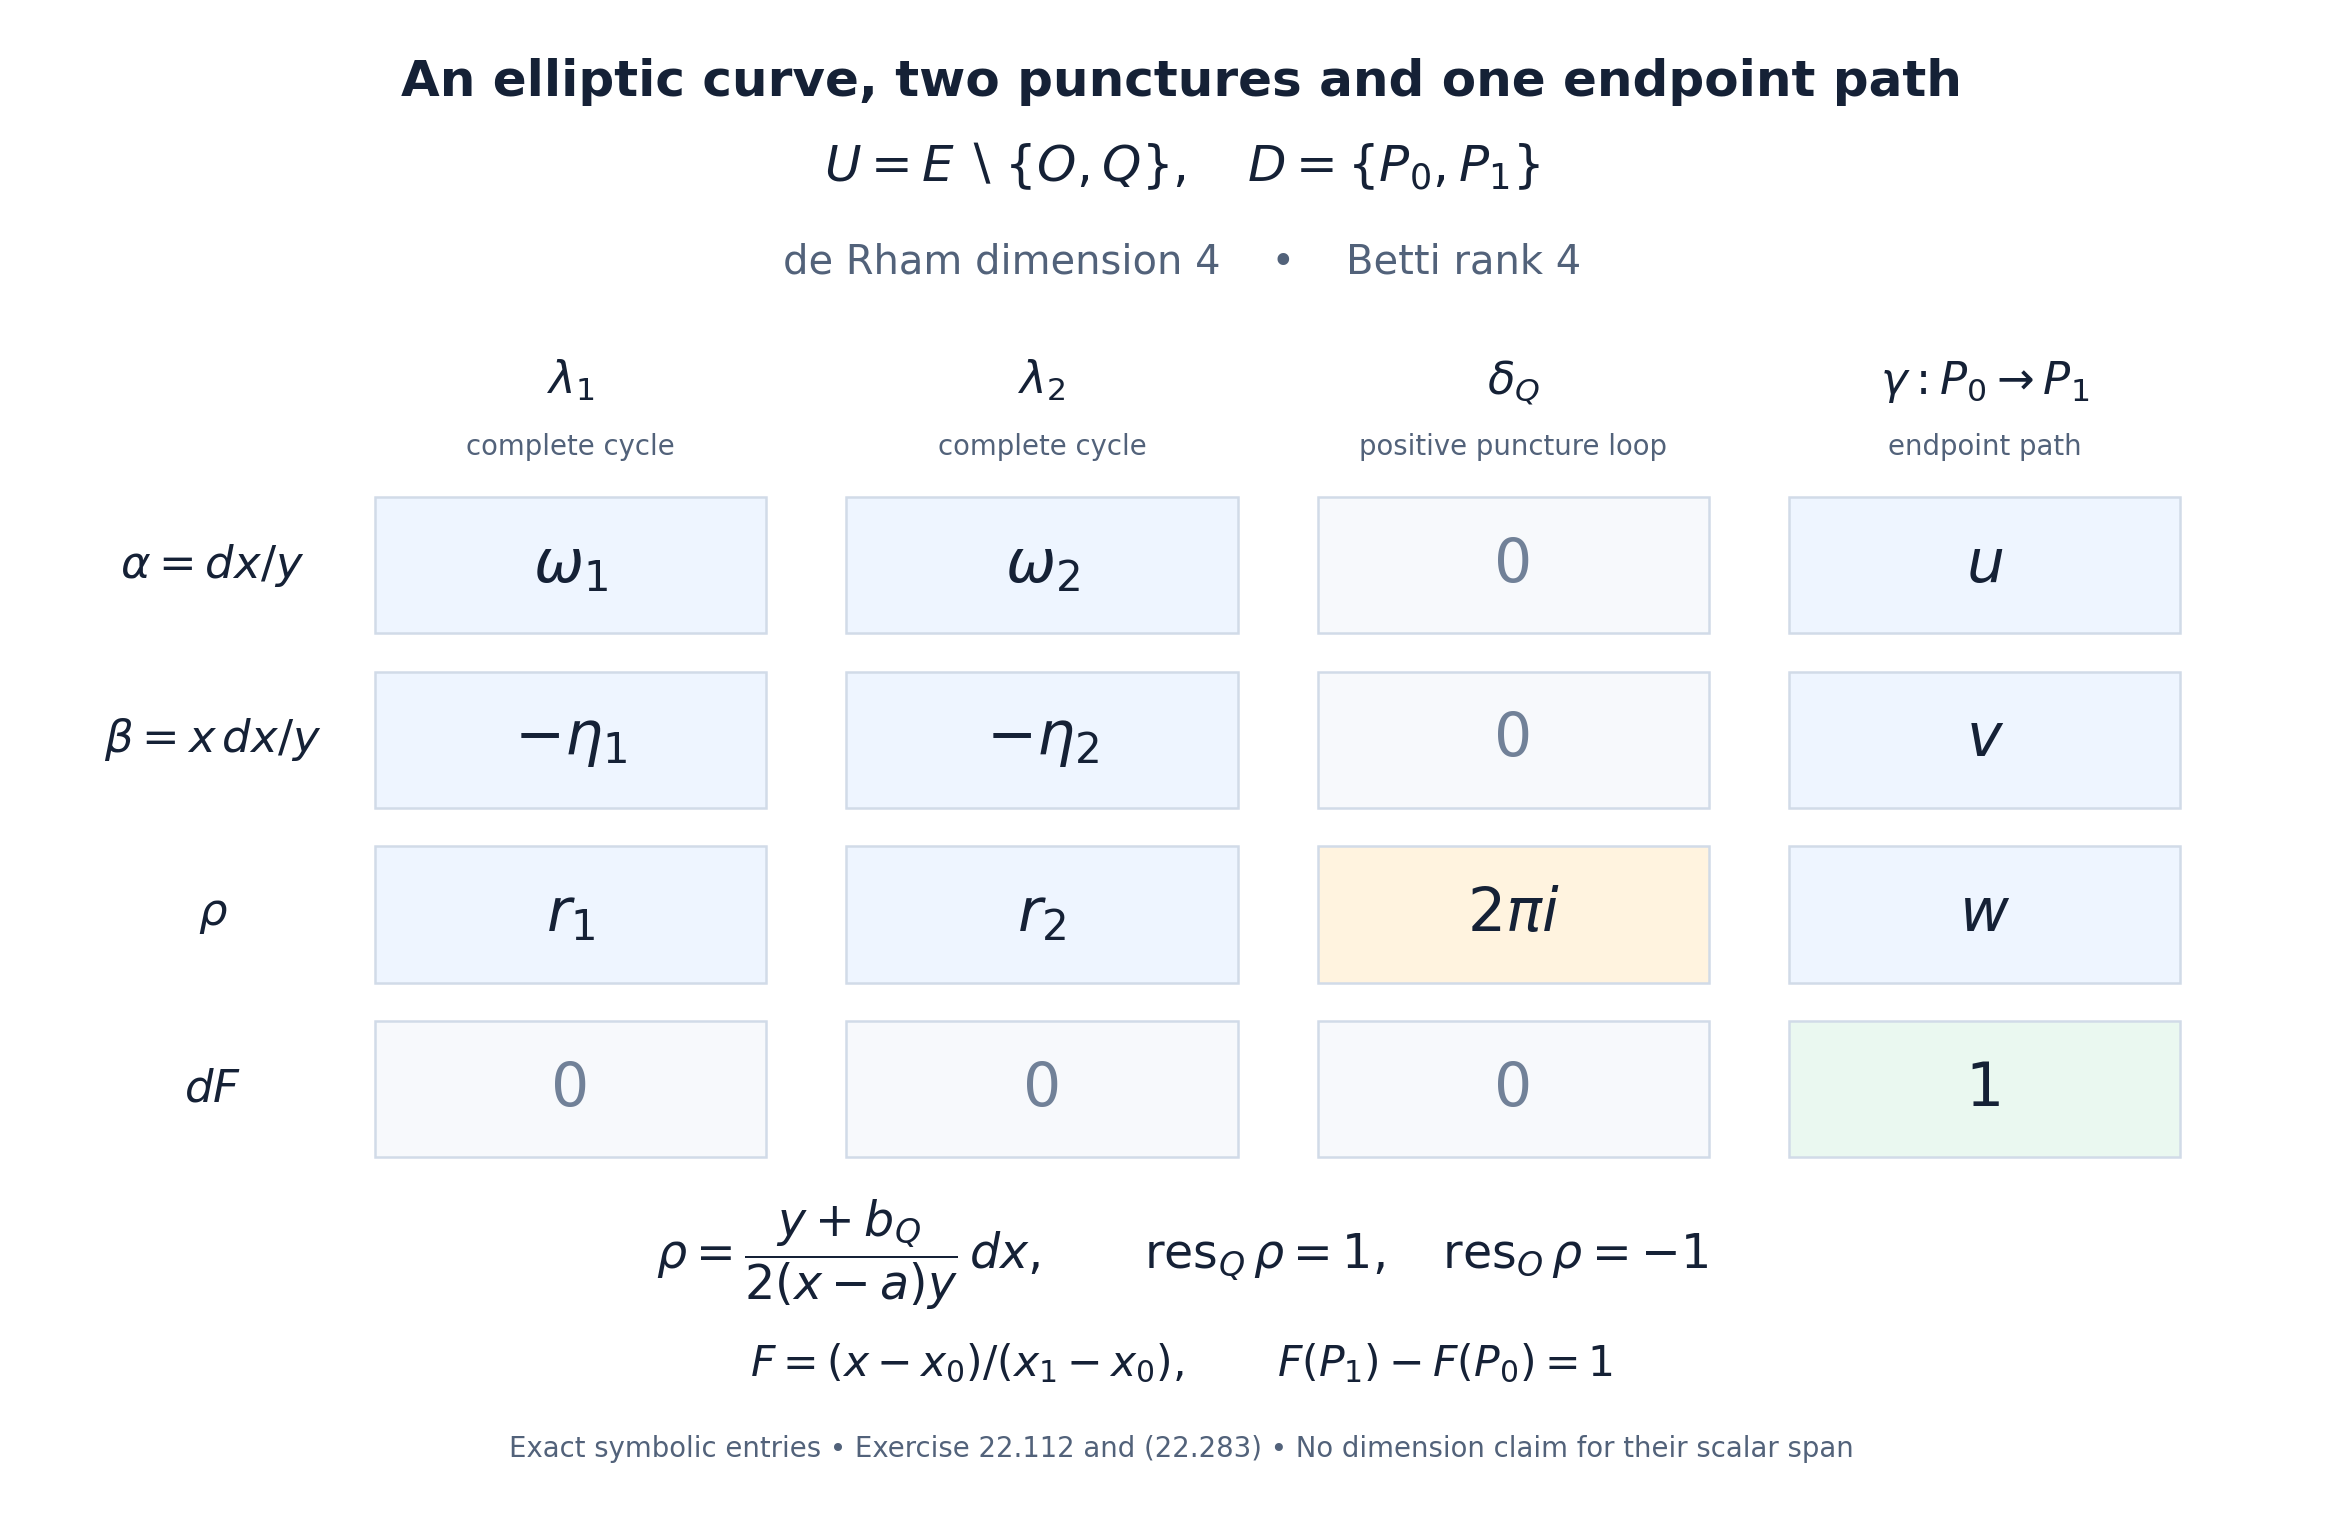
\includegraphics[keepaspectratio,alt={An exact four-by-four period matrix distinguishing complete elliptic cycles, a puncture loop and an endpoint path.}]{../verification/lesson22/elliptic-relative-period-matrix.png}}
\par\smallskip
\begin{flushleft}\small
\emph{Figure 22.8. Exercise 22.112. The small positive loop around \(Q\)
detects the residue \(1\) of \(\rho\); its residue at the other puncture
\(O\) is \(-1\). The endpoint path detects \(F(P_1)-F(P_0)=1\). The two
complete cycles retain the elliptic period and negative quasi-period
entries. The symbols \(u,v,w,r_1,r_2\) denote the corresponding
integrals in (22.283), with no numerical approximation.}
\end{flushleft}
\end{minipage}\par\medskip


For Jacobians and symmetric powers, see J. S. Milne's freely available
author edition of
\href{https://www.jmilne.org/math/xnotes/JVs.pdf}{\emph{Jacobian
Varieties}}, Sections 3--5; Section 8 discusses generalized Jacobians.
The curve-period comparison is treated in Huber and Wüstholz,
\href{https://home.mathematik.uni-freiburg.de/arithgeom/preprints/huber-einsmotive.pdf}{\emph{Transcendence
and linear relations of 1-periods}}, Sections 4.5 and 12.3.

\subsection{Affine filtrations and relative
cohomology}\label{affine-filtrations-and-relative-cohomology}

We work over \(k=\overline{\mathbf Q}\), with its fixed embedding in
\(\mathbf C\). A constructible sheaf below is a sheaf of
finite-dimensional \(\mathbf Q\)-vector spaces on the analytic space of
a variety, locally constant on the members of a finite algebraic
stratification defined over \(k\). Cohomology in this section is
singular or analytic sheaf cohomology with rational coefficients. For a
constant sheaf these agree by the local-cochain comparison in Lemma
22.107.

\subsubsection{Lemma 22.113. A punctured-line calculation in
families}\label{lemma-22.113.-a-punctured-line-calculation-in-families}

Let \(p:\mathbf A^n\to\mathbf A^{n-1}\) be a coordinate projection. Let
\(Z\subset\mathbf A^n\) be a hypersurface finite and surjective over the
base. Suppose that \(F\) is locally constant on
\(\mathbf A^n\setminus Z\) and has zero stalks on \(Z\). Then \[
 R^qp_*F=0\quad(q\ne1),\qquad
 A=R^1p_*F\ \text{is constructible}.
 \tag{22.284}
\] If \(h:V\hookrightarrow\mathbf A^{n-1}\) is an algebraic open
immersion and \(j:p^{-1}V\hookrightarrow\mathbf A^n\), then \[
 Rp_*(j_!j^*F)\simeq h_!h^*(Rp_*F).
 \tag{22.285}
\] For a fibre with \(s\ge1\) distinct points of \(Z\), the only nonzero
possible cohomology group is in degree one. Its dimension is
\((s-1)\operatorname{rank}F\).

\textbf{Proof.} First consider a local system \(L\) on
\(\mathbf C\setminus S\), where \(S\) is finite and nonempty, and extend
it by zero to a sheaf \(G\) on \(\mathbf C\). On a small disc containing
exactly one point of \(S\), this extension has zero cohomology in every
degree. Here the possible monodromy of \(L\) must be retained. For the
punctured-disc inclusion \(a\) and the central-point inclusion \(i\),
the open--closed exact sequence, applied to a resolution, gives the
triangle \[
 a_!L\longrightarrow Ra_*L
       \longrightarrow i_*i^*Ra_*L.
 \tag{22.286}
\] The cohomology of the middle term on the disc is the cohomology of
its punctured disc. The stalk of the last term is the direct limit of
the same cohomology on smaller punctured discs. All restriction maps are
isomorphisms: radial contraction preserves the local system and
identifies each punctured disc with a circle carrying its monodromy. The
map from the middle term to the last term is therefore an isomorphism on
cohomology, proving the assertion.

Join the points of \(S\) by an embedded tree with vertex set \(S\).
Thickening its vertices and edges gives an open disc-shaped
neighbourhood. Cover this neighbourhood by small open vertex regions,
each containing one puncture and the adjacent half-edges. Each region
has the cohomology just computed. Regions meet only along the edges of
the tree; each nonempty intersection is a contractible strip with no
puncture, and there are no triple intersections. The Čech resolution
therefore has zero terms in degree zero and one stalk of \(L\) for each
edge in degree one. There are \(s-1\) edges. Enlarging the neighbourhood
to the plane adds only an outer collar, where \(G\) is locally constant.
Retraction of that collar induces the same cohomology; this can also be
checked by applying (22.286) to the punctures before and after the
retraction. Thus \[
 H^q(\mathbf C,G)=0\ (q\ne1),\qquad
 H^1(\mathbf C,G)\simeq\bigoplus_{\text{tree edges }e}L_{t_e},
 \tag{22.287}
\] where \(t_e\) is an interior point of the edge. The displayed
isomorphism depends on the chosen tree.

We give the base-change detail needed to use this calculation in a
family. A finite morphism is proper. On a sufficiently small relatively
compact neighbourhood \(B\) of a base point, all points of \(Z\) lie
inside a fixed disc \(|z|<R\) in the fibre. Outside a slightly smaller
disc there are no singularities of \(F\). Radial contraction identifies
the sheaf on this outer collar with the pullback of its restriction to
the boundary circle. Restriction from \(\mathbf C\times B\) to the
closed disc \(\{|z|\le R\}\times B\) consequently induces the same
derived direct image. The same assertion holds after extension by zero
from an open subset of \(B\), because this extension changes only the
base variable.

For this compact-disc projection, cohomology commutes with restriction
to a fibre. One elementary form of the required compactness argument is
the following. For a compact closed set \(K\) in a locally compact
metrizable space, and a sheaf \(A\), restriction gives \[
 \underset{W\supset K}{\operatorname{colim}}H^q(W,A)
       \simeq H^q(K,A|_K).
 \tag{22.288}
\] To verify it, compute sheaf cohomology by the direct limit of Čech
complexes over open covers. This computes derived cohomology on these
paracompact spaces: apply the Čech construction to an injective
resolution; its rows are exact in positive Čech degree, and refinements
kill the positive local resolution cohomology. A cover of the compact
set has a finite refinement. Its sets, the sections on their finite
intersections, and any equalities among these sections extend to a
neighbourhood of the compact set, by the definition of the inverse-image
sheaf and another finite refinement. The same argument applies to
cocycles and coboundaries, proving (22.288). Under a proper map, inverse
images of neighbourhoods of a point are cofinal among neighbourhoods of
its fibre: the image of the closed complement of such a neighbourhood is
closed and misses that point. Applying (22.288) therefore gives the
asserted fibre calculation for a proper map.

It follows that the stalks of \(R^qp_*F\) are exactly the groups in
(22.287). This proves their vanishing outside degree one. It also proves
(22.285): on the compact-disc model the natural base-change morphism is
an isomorphism on every stalk. At a point of \(V\) it is the identity
fibre calculation, and at a point outside \(V\) both fibre sheaves are
zero.

Finally stratify the base so that the reduced finite map from \(Z\) is a
finite étale cover on each stratum. Such a finite stratification is
obtained by taking its étale locus over a smooth dense open of each
image component and repeating on the remaining smaller closed sets;
characteristic zero makes the generic field extensions separable. In a
small analytic ball in a stratum the punctures can be labelled and moved
continuously without collision. Disjoint small discs and bump functions
extend this motion to a homeomorphism of the whole fibre, equal to the
identity outside a large disc. The local system on the complement and
the tree computation are therefore locally constant in that ball. This
proves constructibility of \(R^1p_*F\). \(\square\)

\subsubsection{Theorem 22.114. The affine filtration
lemma}\label{theorem-22.114.-the-affine-filtration-lemma}

Let \(X\) be an affine variety of dimension \(n\) and \(F\) a
constructible sheaf on \(X\). There is an algebraic open
\(j:U\hookrightarrow X\), with \(\dim(X\setminus U)<n\), such that \[
 H^q(X,j_!j^*F)=0\qquad(q\ne n).
 \tag{22.289}
\] All these groups are finite-dimensional. In particular, for every
closed \(W\subset X\) of dimension less than \(n\), there is a closed
\(Z\supset W\), also of dimension less than \(n\), such that \[
 H^q(X,Z;\mathbf Q)=0\qquad(q\ne n).
 \tag{22.290}
\] The open \(X\setminus Z\) may be required to be smooth.

\textbf{Proof.} We use
\href{../AG-CA/AG-CA-09.html\#3-normalization-that-respects-ideals}{\emph{Krull
dimension and Noether normalization}, Corollary 3.2 and Theorem 4.2}.
They give a finite surjection \(\pi:X\to\mathbf A^n\). For a finite map,
direct image is exact and its stalk at \(y\) is
\(\bigoplus_{x\in\pi^{-1}(y)}F_x\). Indeed a finite fibre has disjoint
neighbourhoods, and properness makes their union contain the full
inverse image of a sufficiently small base neighbourhood. This
identifies the stalk with that finite sum, an exact operation. The same
observation gives \(\pi_*j_!j^*F=v_!v^*\pi_*F\) when \(U=\pi^{-1}(V)\).
Direct image preserves constructibility: stratify the finite map into
finite étale pieces, refine by the strata of \(F\), and use the local
finite-sheet description on each piece. A closed subset of dimension
less than \(n\) has a preimage of dimension less than \(n\) under a
finite map, by dimension preservation for integral extensions. It
therefore suffices to prove the theorem on \(\mathbf A^n\).

Induct on \(n\). For \(n=0\) there is a finite set of points and no
positive cohomology. For \(n>0\), choose a nonzero nonconstant
polynomial \(f\) such that \(F\) is locally constant on its complement.
Replace \(F\) by its restriction to that complement, extended by zero.
This is allowed: successive restrictions and extensions by zero along
open immersions compose. It will only enlarge the final exceptional set
by \(V(f)\).

A change of coordinates makes \(f\) monic of positive degree in the last
coordinate; Lemma 2.1 of the cited normalization lesson proves this
directly. Thus \(V(f)\to\mathbf A^{n-1}\) is finite and surjective.
Lemma 22.113 says that its projection has only one nonzero higher direct
image, the constructible sheaf \(A=R^1p_*F\). The cohomology spectral
sequence for composition of sections and direct image reduces to \[
 H^q(\mathbf A^n,F)\simeq H^{q-1}(\mathbf A^{n-1},A).
 \tag{22.291}
\] This spectral sequence can be obtained by an injective resolution
followed by a resolution for sections; with only one cohomology row its
total complex has the displayed cohomology.

Apply the induction hypothesis to \(A\). It supplies an open \(V\) of
the base on which extension by zero has cohomology only in degree
\(n-1\). Equation (22.285) and (22.291) show that restricting the
original sheaf to \(p^{-1}V\setminus V(f)\) and extending by zero has
cohomology only in degree \(n\). The excluded set is the union of
\(V(f)\) and the inverse image of a set of dimension at most \(n-2\), so
has dimension less than \(n\). Finite-dimensionality follows at each
step from (22.287), ending with finitely many finite-dimensional stalks
in dimension zero. This proves (22.289).

For (22.290), take \(F=a_!\mathbf Q_{X\setminus W}\). The resulting
extension by zero is the constant sheaf on \(U\setminus W\), extended by
zero to \(X\). Its cohomology is relative cohomology for the closed
complement \(Z=W\cup(X\setminus U)\): the exact sequence
\(0\to j_!\mathbf Q\to\mathbf Q_X\to\mathbf Q_Z\to0\) identifies its
resolved sections with the shifted relative cone. Enlarge \(W\) first by
the singular locus and all components of dimension less than \(n\), if
smoothness is desired. These added sets have dimension less than \(n\);
the remaining open is smooth. \(\square\)

\subsubsection{Proposition 22.115. Compatible filtrations and the
degree-one
complex}\label{proposition-22.115.-compatible-filtrations-and-the-degree-one-complex}

For an affine variety \(X\) of dimension \(n\) and a closed subvariety
\(Y\), there are compatible filtrations \[
 \varnothing=X_{-1}\subset X_0\subset\cdots\subset X_n=X,
 \qquad
 \varnothing=Y_{-1}\subset Y_0\subset\cdots\subset Y_n=Y,
 \qquad Y_i\subset X_i,
 \tag{22.292}
\] with \(\dim X_i,\dim Y_i\le i\), smooth differences, and
\(H^q(X_i,X_{i-1})=H^q(Y_i,Y_{i-1})=0\) for \(q\ne i\). The cohomology
of \(X\) is computed by \[
 C(X_\bullet)=
 [H^0(X_0)\longrightarrow H^1(X_1,X_0)
   \longrightarrow H^2(X_2,X_1)\longrightarrow\cdots],
 \tag{22.293}
\] with the connecting maps of triples as differentials. The shifted
cone of \(C(X_\bullet)\to C(Y_\bullet)\) computes \(H^*(X,Y)\). In
particular \(H^1(X,Y)\) is a subquotient of \[
 H^1(X_1,X_0)\oplus H^0(Y_0).
 \tag{22.294}
\]

\textbf{Proof.} Apply Theorem 22.114 successively to construct the
filtration of \(Y\) downwards, padding by repetitions whenever its
dimension is smaller than the index. Construct that of \(X\) downwards
next. In choosing \(X_{i-1}\) inside \(X_i\) of dimension \(i\), require
it to contain \(Y_{i-1}\), the singular locus of \(X_i\), and its
smaller-dimensional components. This is an allowed closed set of
dimension at most \(i-1\). If \(\dim X_i<i\), take \(X_{i-1}=X_i\). Its
relative group is zero in every degree, and it still contains
\(Y_{i-1}\). The construction gives all stated properties.

Filter the singular cochain complex by restriction to the successive
closed sets. The long exact sequences of successive pairs form the exact
couple whose first page is \(E_1^{i,j}=H^{i+j}(X_i,X_{i-1})\). The
vanishing just proved leaves only \(j=0\). Its first differential is the
connecting map in (22.293); every higher differential enters or leaves a
zero row. Hence its cohomology is naturally \(H^*(X)\). This argument is
also seen directly by successively taking the cones for the restriction
maps and cancelling the acyclic degrees of each relative complex.

Apply the same filtered construction to the map from the cochain complex
of \(X\) to that of \(Y\). Equivalently take its double complex and then
the shifted cone. The degree-zero, degree-one and degree-two terms of
the resulting complex are \[
 H^0(X_0),\quad
 H^1(X_1,X_0)\oplus H^0(Y_0),\quad
 H^2(X_2,X_1)\oplus H^1(Y_1,Y_0).
 \tag{22.295}
\] The signs are those of the shifted cone. Its degree-one cohomology is
a kernel modulo an image inside the middle term, giving (22.294).
\(\square\)

\subsubsection{Proposition 22.116. An affine replacement by affine-space
bundles}\label{proposition-22.116.-an-affine-replacement-by-affine-space-bundles}

Every quasiprojective variety \(X\) has a diagram \[
 T\longrightarrow X'\longrightarrow X
 \tag{22.296}
\] in which \(T\) is affine and both arrows are Zariski locally trivial
affine-space bundles with affine-linear transition functions. On
analytic spaces both arrows are homotopy equivalences, including for
pairs obtained by inverse image of a closed subset. If \(X\) is smooth,
the arrows also induce isomorphisms on algebraic de Rham cohomology.

\textbf{Proof.} Embed \(X\) as a locally closed subvariety of
\(\mathbf P^N\). Consider pairs \((\ell,H)\) of a line
\(\ell\subset k^{N+1}\) and a hyperplane not containing that line. This
incidence complement \(J\) is affine. Explicitly, it is the closed
affine variety of \((N+1)\)-square matrices whose two-by-two minors
vanish and whose trace is one: send a line vector \(x\) and covector
\(a\), with \(a(x)\ne0\), to \(xa/a(x)\). Conversely a rank-one matrix
of trace one has an image line and a kernel hyperplane which are
complementary. These maps are regular on the usual nonzero-coordinate
charts and inverse to each other.

The projection \(J\to\mathbf P^N\) has fibre \(\mathbf A^N\). On a chart
where a coordinate of \(x\) is one, normalize \(a(x)=1\); the other
\(N\) covector coordinates are free. Changing charts gives affine-linear
changes in those coordinates. Its pullback \(X'\to X\) is such a bundle.
Moreover \(X'\) is locally closed in the affine variety \(J\), so is an
open subset of its affine closure \(V\).

Let \(f_1,\ldots,f_m\) generate the ideal of \(V\setminus X'\) in \(V\).
If the complement is empty, use \(m=1,f_1=1\). The variety \[
 T=\{(v,t_1,\ldots,t_m)\in V\times\mathbf A^m:
                     \textstyle\sum_i f_i(v)t_i=1\}
 \tag{22.297}
\] is affine and maps into \(X'\). Over the open set \(f_i\ne0\), solve
for \(t_i\); this gives a trivial affine-space bundle of rank \(m-1\).
Differences of two solutions form the kernel vector bundle of the
surjection \(\mathcal O_{X'}^m\to\mathcal O_{X'}\) given by the \(f_i\).
Thus the transitions are affine-linear.

For either arrow, local continuous sections can be combined using a
partition of unity, since affine combinations in each fibre are defined
independently of coordinates. Contraction towards the resulting section
is a homotopy equivalence. It preserves the inverse image of any closed
subset of the base, proving the assertion for pairs. For smooth \(X\),
both total spaces are smooth and Proposition 22.84 applies to their
vector-bundle torsors. One can see the de Rham assertion on each
trivializing chart by integrating polynomial fibre forms, and then use
the Čech double complex to glue these local quasi-isomorphisms.
\(\square\)

\subsubsection{Exercise 22.117. An affine surface with one relative
degree-two
class}\label{exercise-22.117.-an-affine-surface-with-one-relative-degree-two-class}

In \(X=\mathbf A^2_{t,z}\), let \[
 Y=V\bigl((z^2-t)(t-1)\bigr).
 \tag{22.298}
\] Compute \(H^q(X,Y;\mathbf Q)\), and give a compatible filtration
exhibiting the class in degree two.

\textbf{Solution.} Write \(P=V(t-z^2)\) and \(L=V(t-1)\). Each is an
affine line, hence analytically contractible, and their intersection
consists of \(A=(1,-1)\) and \(B=(1,1)\). For the closed cover
\(Y=P\cup L\), the sheaf sequence \[
 0\longrightarrow\mathbf Q_Y
 \longrightarrow\mathbf Q_P\oplus\mathbf Q_L
 \longrightarrow\mathbf Q_{\{A,B\}}\longrightarrow0
 \tag{22.299}
\] is exact on every stalk; the last arrow is the difference of
restrictions. Its map on degree-zero cohomology sends \((a,b)\) to
\((a-b,a-b)\). Its kernel and cokernel both have dimension one. Higher
cohomology of the three pieces is zero. Thus \(H^0(Y)=\mathbf Q\),
\(H^1(Y)=\mathbf Q\), and all other groups vanish. Since
\(X(\mathbf C)\) is contractible and \(Y\) is connected, the relative
sequence gives \[
 H^q(X,Y;\mathbf Q)=
 \begin{cases}\mathbf Q,&q=2,\\0,&q\ne2.\end{cases}
 \tag{22.300}
\]

Take \(X_2=X\), \(X_1=Y\), and \(X_0=\{A,B\}\). The open
\(Y\setminus\{A,B\}\) is smooth, as is \(X\setminus Y\). The pair
\((Y,\{A,B\})\) has only degree-one cohomology, of dimension two: its
relative sequence has one endpoint difference and one loop class. The
complex (22.293) is therefore \(\mathbf Q^2\to\mathbf Q^2\to\mathbf Q\).
The first map has rank one and the second is surjective; its kernel is
the first image. This follows either from the exact sequence of the
triple or from the contractibility of \(X\) just used. Its only
cohomology is one copy of \(\mathbf Q\) in degree zero, as required.

The relative generator is detected by a loop in \(Y\) travelling from
\(A\) to \(B\) on \(P\) and back on \(L\). No nonzero class in
\(H^1(X,Y)\) results from this loop: the boundary map places it in
degree two.

\begin{minipage}[t]{\linewidth}
\centering
\pandocbounded{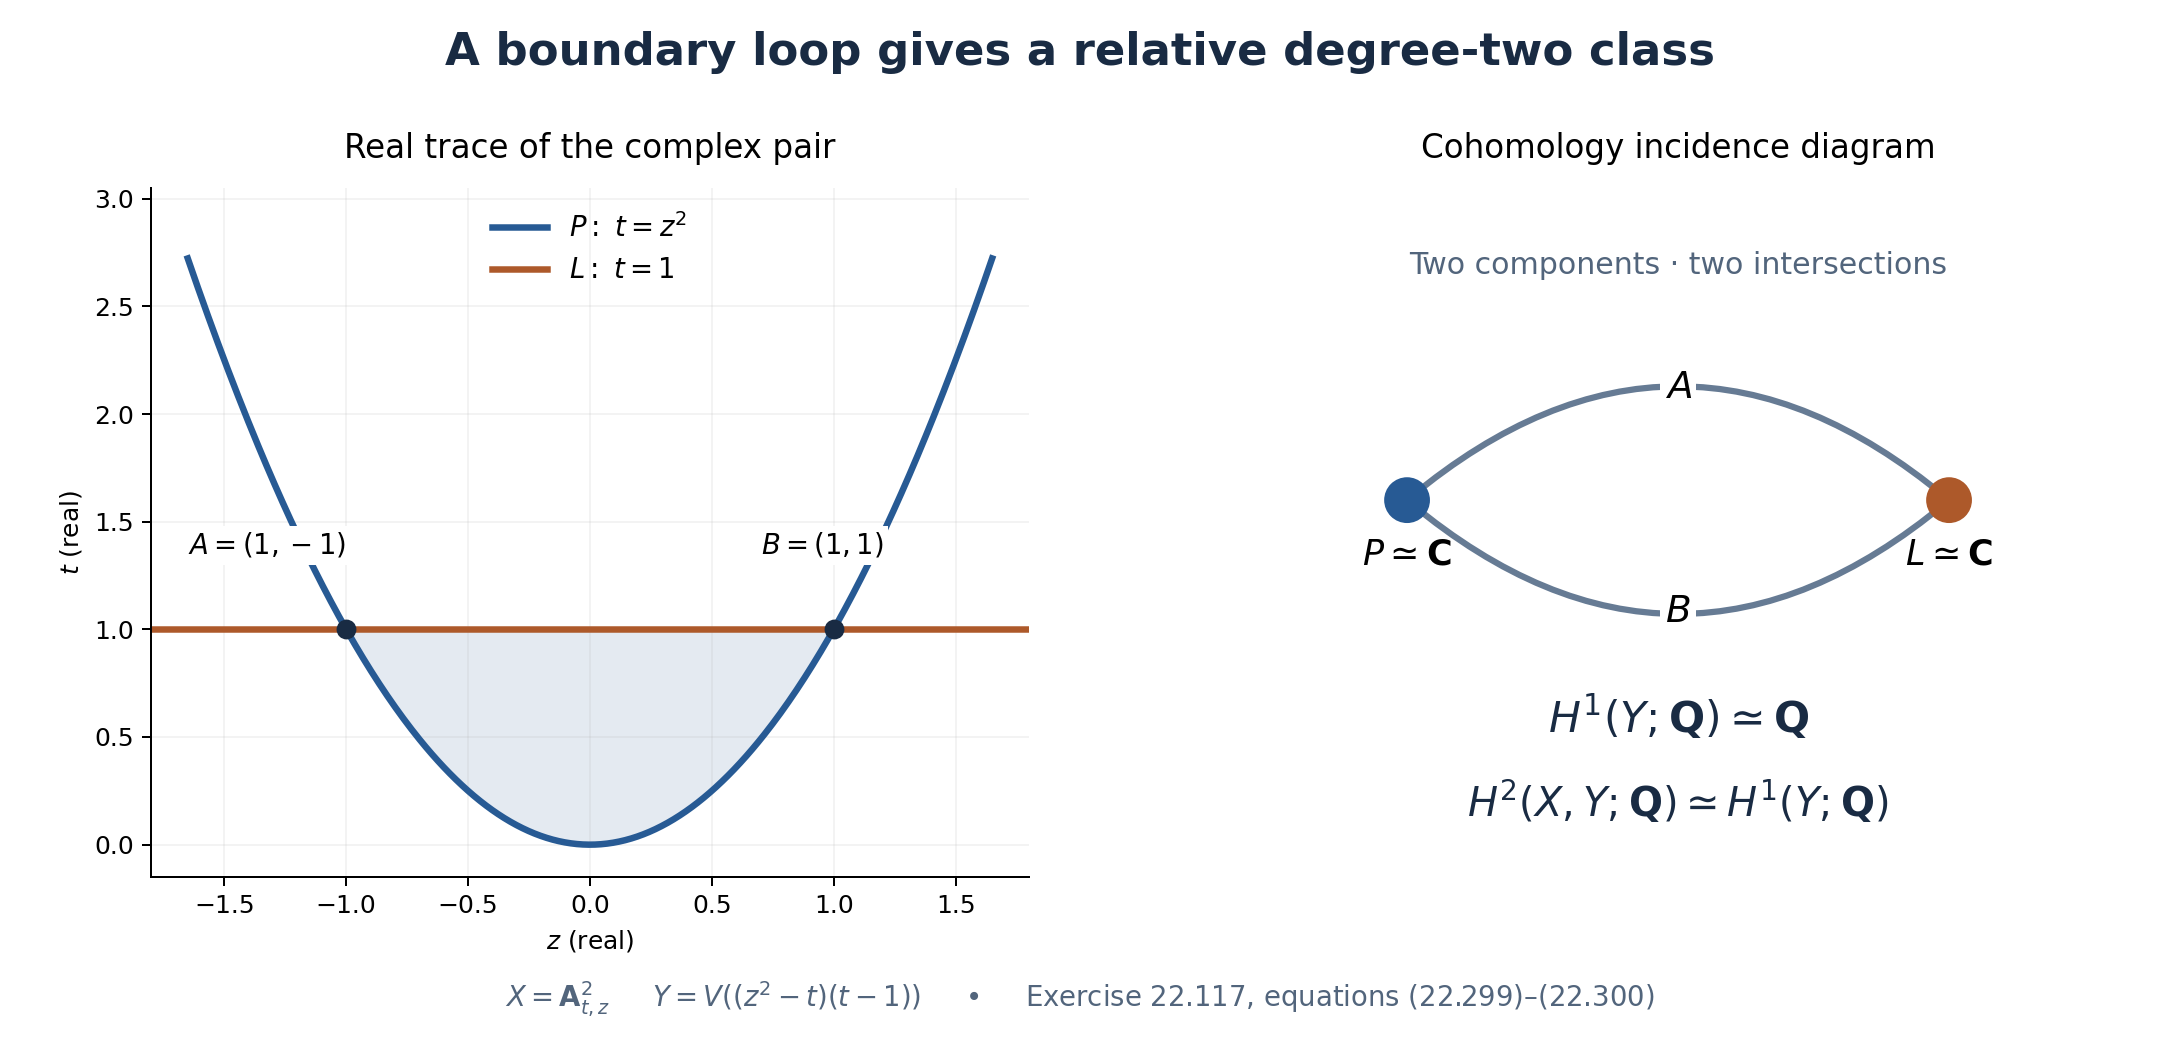
\includegraphics[keepaspectratio,alt={The real traces of a parabola and a line meet twice; their two paths form the loop which determines the relative degree-two class.}]{../verification/lesson22/affine-filtration-pair.png}}
\par\smallskip
\begin{flushleft}\small
\emph{Figure 22.9. Exercise 22.117. The left panel shows the real trace
inside the complex affine surface; point labels use the coordinate order
\((t,z)\). The right panel records the two contractible components and
their two intersection points. The loop represents the one-dimensional
\(H^1(Y)\); the relative sequence identifies it with \(H^2(X,Y)\).}
\end{flushleft}
\end{minipage}\par\medskip


The filtration argument is due to Nori. A freely accessible account is
Huber and Müller-Stach,
\href{https://home.mathematik.uni-freiburg.de/arithgeom/preprints/buch-alt/buch-v6.pdf}{\emph{Periods
and Nori Motives}, author edition}, Section 2.5.3. The affine
replacement above is an explicit form of the affine-space bundle
construction commonly called Jouanolou's construction.

\subsection{Comparison on open varieties, descent, and degree-one
periods}\label{comparison-on-open-varieties-descent-and-degree-one-periods}

In this section a variety is a reduced quasiprojective scheme over
\(k=\overline{\mathbf Q}\). Products and inverse images are given their
reduced structures. This convention does not change the analytic spaces
or their singular cohomology. A comparison object consists of
finite-dimensional spaces over \(k\) and \(\mathbf Q\), together with an
isomorphism between their extensions to \(\mathbf C\). Maps respect both
rational structures and this isomorphism. Kernels and cokernels are
taken over the two respective fields. Extension of scalars is exact, so
these again are comparison objects.

\subsubsection{Lemma 22.118. Removing poles from the logarithmic
complex}\label{lemma-22.118.-removing-poles-from-the-logarithmic-complex}

Let \(U\) be smooth. There is a natural isomorphism \[
 H^q_{\mathrm{dR}}(U/k)\otimes_k\mathbf C
       \simeq H^q(U(\mathbf C),\mathbf Q)\otimes_{\mathbf Q}\mathbf C.
 \tag{22.301}
\] It is integration on classes represented by differential forms. Both
spaces before extension of scalars are finite dimensional.

\textbf{Proof.} Choose a smooth projective compactification \(P\) of
\(U\) whose boundary \(D=P\setminus U\) is a divisor with simple normal
crossings. This is
\href{../resolution-of-singularities-in-characteristic-zero/principalization-and-resolution.html\#5-consequences-used-in-the-programme}{Corollary
5.2 of the resolution course}. Its quasiprojective case starts with
projective closure, resolves that closure away from \(U\), and
principalizes the boundary away from \(U\). Write
\(j:U\hookrightarrow P\).

Here is the algebraic comparison with the logarithmic complex, including
the local contraction. Near a point of \(D\), choose étale coordinates
\(t_1,\ldots,t_d\) with \(D=V(t_1\cdots t_r)\). The complex
\(L=\Omega^\bullet_P(\log D)\) has exterior generators \(dt_i/t_i\) for
\(i\le r\), and \(dt_i\) for \(i>r\). Invert the boundary coordinates
one at a time. At the step involving \(t=t_i\), other already inverted
coordinates are included in the coefficient ring. For every \(m>0\), the
quotient \[
 t^{-m}L/t^{-(m-1)}L
       \simeq (L/tL,\ \bar d-m\theta\wedge-),\qquad
 \theta=dt/t,
 \tag{22.302}
\] is an isomorphism of complexes of \(k\)-vector spaces, with the
differential displayed on the right. Put \(e=t\partial/\partial t\). The
coordinate derivation extends through the étale coordinate map. On
\(L/tL\), Cartan's identity gives \(\bar d\,\iota_e+\iota_e\bar d=0\):
the Lie derivative kills the exterior generators and sends each
coefficient into \(tL\). Also
\(\theta\wedge\iota_e+\iota_e\theta\wedge=1\). Consequently the
differential \(D_m\) on the right of (22.302) satisfies \[
 D_m(-\iota_e/m)+(-\iota_e/m)D_m=1.
 \tag{22.303}
\] The quotient is contractible. Induction on the finite pole order,
followed by the union over \(m\), proves \(L\simeq L[t_i^{-1}]\). Doing
this for all \(i\le r\) proves \[
 \Omega^\bullet_P(\log D)\simeq j_*\Omega^\bullet_U.
 \tag{22.304}
\] This argument uses pole-order quotients; it requires no expansion of
an algebraic coefficient as a Laurent polynomial. The immersion \(j\) is
affine: on a boundary chart it is the principal open set
\(t_1\cdots t_r\ne0\). Thus its higher direct images on the
quasi-coherent terms vanish, and (22.304) computes
\(H^*_{\mathrm{dR}}(U/k)\).

On a complex polydisc, the analytic logarithmic complex has local
cohomology the exterior algebra on the constant classes
\(dt_1/t_1,\ldots,dt_r/t_r\). To verify this, first use the holomorphic
Poincaré contraction in the nonboundary coordinates. Expand the
remaining holomorphic coefficients into convergent power series in the
boundary coordinates. A nonconstant monomial of multiweight
\(\nu\in\mathbf N^r\) is contracted by
\(\iota_{t_i\partial/\partial t_i}/\nu_i\), choosing the first \(i\)
with \(\nu_i>0\). The denominators have absolute value at least one, so
these operations preserve convergence on every smaller polydisc.
Constant coefficients leave exactly the stated exterior algebra. The
punctured polydisc retracts onto \((S^1)^r\); integration of the
indicated generators around its coordinate circles is \(2\pi i\). Their
exterior products therefore give all its cohomology. This proves that
the analytic logarithmic complex computes \(Rj_*\mathbf C_U\). The
holomorphic Poincaré argument and the local singular-cochain resolution
are the ones used in Lemma 22.107.

Each term of the logarithmic complex is coherent on the projective
variety \(P\). The
\href{../AG-QC/serres-comparison-theorems-and-chows-theorem.html\#3-the-first-comparison-theorem}{coherent
cohomology comparison theorem}, applied term by term and then to the
bounded hypercohomology spectral sequence, identifies its algebraic and
analytic hypercohomology after scalar extension. Coherent cohomology on
\(P\) is finite dimensional. Combining the two logarithmic comparisons
proves (22.301) and finiteness.

The map just proved to be an isomorphism is the canonical map from
algebraic forms to analytic forms, followed by the analytic de Rham
comparison. Hence it is independent of \(P\) and is natural for
morphisms between smooth varieties. In particular the proof does not
require a chosen morphism to extend to the chosen compactifications.
\(\square\)

\subsubsection{Lemma 22.119. Descent for a proper Čech
cover}\label{lemma-22.119.-descent-for-a-proper-ux10dech-cover}

Let \(p:V\to X\) be proper and surjective, and set
\(V_n=V\times_X\cdots\times_XV\), with \(n+1\) factors. Then the
augmentation induces a quasi-isomorphism \[
 R\Gamma(X(\mathbf C),\mathbf Q)
       \simeq
 \operatorname{Tot}_{n\ge0}R\Gamma(V_n(\mathbf C),\mathbf Q).
 \tag{22.305}
\] The differential in the new degree is the alternating sum of the
pullbacks along the maps omitting one factor. The assertion holds after
every algebraic base change.

\textbf{Proof.} Use the nonnegative sheaf resolutions for singular
cohomology from Lemma 22.107 and form the augmented complex of derived
direct images on \(X(\mathbf C)\). Its totalization has only finitely
many terms on each diagonal. By the compact-fibre base-change argument
(22.288), its stalk at \(x\) is computed by the augmented cosimplicial
cochain complex of \[
 F,\ F^2,\ F^3,\ldots,\qquad F=p^{-1}(x)(\mathbf C).
 \tag{22.306}
\] In this calculation the augmentation is the cochain complex of one
point. Every map \(V_n\to X\) is proper, so the same base-change
argument applies in every degree, compatibly with the face maps.

The compact space \(F\) is nonempty. Fix \(a\in F\). Insertion of \(a\)
as the first coordinate gives \(F^n\to F^{n+1}\), including the map from
a point to \(F\). On cochains its pullback \(h\) satisfies
\(\delta h+h\delta=1\) in the augmented cosimplicial direction. Indeed
the term deleting the inserted coordinate is the identity; every other
deletion cancels the corresponding term with the opposite sign. This
calculation also applies to cohomology in each vertical degree. Thus the
augmented first-page rows of the double-complex spectral sequence are
exact. The total augmentation is a quasi-isomorphism.

A morphism of sheaf complexes inducing isomorphisms on all stalk
cohomology is a quasi-isomorphism. Taking derived global sections proves
(22.305). Properness and surjectivity persist under base change, proving
the last assertion. The chosen point is used only on a fibre; no local
section of \(p\) is assumed. \(\square\)

\subsubsection{Lemma 22.120. From Čech descent to hypercover
descent}\label{lemma-22.120.-from-ux10dech-descent-to-hypercover-descent}

Suppose that a presheaf \(K^\bullet\) of complexes on a site vanishes in
all degrees below one fixed integer. Suppose that for every covering and
its base changes, the augmented Čech totalization computes \(K^\bullet\)
on the covered object. Then every hypercover \(U_\bullet\to X\) computes
it: \[
 K^\bullet(X)\simeq
       \operatorname{Tot}K^\bullet(U_\bullet).
 \tag{22.307}
\] For a family of objects, the expression on the right uses the product
over its members.

\textbf{Proof.} Let \(aK^\bullet\) be the associated complex of sheaves.
Sheafification is exact. Choose a quasi-isomorphism
\(aK^\bullet\to I^\bullet\), with \(I^\bullet\) a bounded-below complex
of injective sheaves. Regard its sections as a presheaf complex and form
\(A^\bullet=\operatorname{Cone}(K^\bullet\to I^\bullet)\). The complexes
\(A^\bullet\) have a uniform lower bound. Their cohomology presheaves
have zero associated sheaves, because sheafification of this cone is
acyclic.

Injective sheaves have exact augmented Čech complexes: the augmented
free abelian sheaf complex of a covering is exact, and applying
\(\operatorname{Hom}(-,I^q)\) is exact. Thus \(I^\bullet\), and hence
also \(A^\bullet\), satisfies the stated Čech descent condition. We
prove by induction that \(H^n(A^\bullet(T))=0\) for every object \(T\).
Start below the uniform lower bound. Suppose the assertion is known in
all degrees below \(n\), on every object. For a cover
\(T_\bullet\to T\), the Čech spectral sequence has first page
\(H^q(A^\bullet(T_p))\). All rows with \(q<n\) vanish. Its edge map is
therefore injective in degree \(n\): \[
 H^n(A^\bullet(T))
       \hookrightarrow H^n(A^\bullet(T_0)).
 \tag{22.308}
\] Any chosen class on the left becomes zero after some cover, since its
cohomology presheaf has zero associated sheaf. Apply (22.308) to that
cover. The original class is zero, which completes the induction.
Consequently \(K^\bullet(T)\to I^\bullet(T)\) is a quasi-isomorphism for
every \(T\).

For a hypercover, the augmented free abelian sheaf complex is again
exact. This follows by filling a finite simplicial boundary locally and
coning each finite-support cycle; the complete construction is
\href{../ag-etale-cohomology/hypercoverings.html\#3-hypercoverings-fill-locally}{Theorem
3.3 of the hypercovering lesson}. Applying the injectives \(I^q\) shows
\(I^\bullet(X)\simeq\operatorname{Tot}I^\bullet(U_\bullet)\), exactly as
in
\href{../ag-etale-cohomology/hypercoverings.html\#4-the-cochain-complex-and-its-comparison}{Theorem
4.1 there}. Replace each evaluated \(I^\bullet\) by \(K^\bullet\). The
resulting total maps are quasi-isomorphisms: after a fixed shift the
double complexes lie in the first quadrant, so the spectral sequences
converge with finite diagonals. This proves (22.307). \(\square\)

Apply this lemma on the category of varieties with the pretopology whose
coverings are the single proper surjective morphisms. They contain
identities and are stable under composition and base change. Take for
\(K^\bullet(T)\) a functorial singular cochain complex of
\(T(\mathbf C)\). Lemma 22.119 supplies Čech descent. We obtain \[
 H^*(X(\mathbf C),\mathbf Q)
   \simeq H^*\!\left(\operatorname{Tot}
                  R\Gamma(U_\bullet(\mathbf C),\mathbf Q)\right)
 \tag{22.309}
\] for every proper hypercover. This application uses the associated
complex \(aK^\bullet\); it does not identify that complex with the
constant sheaf on the proper-cover site.

\subsubsection{Theorem 22.121. De Rham comparison for varieties and
pairs}\label{theorem-22.121.-de-rham-comparison-for-varieties-and-pairs}

Every variety \(X\) has algebraic de Rham cohomology defined by a smooth
proper hypercover. It is independent of that choice, is contravariantly
functorial, and agrees with the usual de Rham cohomology for smooth
\(X\). For a closed subvariety \(Y\subset X\), the relative complex is
the shifted cone of restriction. There are natural comparison
isomorphisms \[
 H^q_{\mathrm{dR}}(X,Y)\otimes_k\mathbf C
       \simeq H^q(X(\mathbf C),Y(\mathbf C);\mathbf Q)
                         \otimes_{\mathbf Q}\mathbf C.
 \tag{22.310}
\] They respect the long exact sequences of pairs and triples, and
finite closed filtrations. All these groups are finite dimensional.

\textbf{Proof.} We first give the construction and its refinements. A
proper hypercover has a proper surjective map to the matching object in
each degree. In degree zero resolve the irreducible components of \(X\)
and take their disjoint union. Resolution is supplied by
\href{../resolution-of-singularities-in-characteristic-zero/principalization-and-resolution.html\#4-resolution-of-singularities}{Theorem
4.8 of the resolution course}. Suppose the smooth levels below \(n\)
have been constructed. Their matching object is a finite limit of
varieties proper over \(X\). Resolve its reduced irreducible components
and use their disjoint union as the new nondegenerate part of level
\(n\). Add a copy of each earlier nondegenerate part for every
surjection \([n]\twoheadrightarrow[j]\), \(j<n\). These are the
prescribed degenerate simplices. Their face maps are determined by
factoring compositions of increasing maps as a surjection followed by an
injection. This factorization is unique, so the simplicial identities
hold. The map from the new level to the matching object is proper and
surjective. This constructs a split smooth proper hypercover
\(U_\bullet\to X\).

There is a relative version of the construction. Given a hypercover
\(V_\bullet\to Z\) and \(f:X\to Z\), resolve in degree \(n\) the
relative matching target \[
 M_nU\times_{M_n(X\times_ZV_\bullet)}
                         (X\times_ZV_n).
 \tag{22.311}
\] Its projection to \(M_nU\) is proper and surjective. With the same
degenerate copies, this gives a smooth hypercover of \(X\) and a map to
\(V_\bullet\). In particular two smooth hypercovers of \(X\) have a
common smooth refinement: apply the construction to their product over
\(X\). Any two parallel maps become simplicially homotopic after a
further hypercover refinement. To see this, use the path object
\(V_\bullet^{\Delta^1}\to
V_\bullet^{\partial\Delta^1}\); its relative matching maps are proper
covers by successive filling of the finitely many simplices of the
prism. Pull it back along the two maps and then make it smooth by
(22.311). The filling and prism identities are proved in
\href{../ag-etale-cohomology/hypercoverings.html\#6-maps-become-homotopic-after-refinement}{Theorem
6.1 of the hypercovering lesson}. That proof uses only stability of
coverings under finite products and base change, so applies to proper
covers.

For smooth \(T\), choose the functorial cochain model of
\(R\Gamma(T,\Omega^\bullet_T)\) obtained by resolving its sheaf complex.
For example, the resolution by products of stalks, with its
coaugmentation and successive cokernels, gives a Godement model.
Pullback of germs and of forms gives the natural maps for a morphism;
the cosimplicial version and its total complex preserve composition.
Apply this simultaneously to all levels and set \[
 R_{\mathrm{dR}}(X)
   =\operatorname{Tot}_{p\ge0}
                R\Gamma(U_p,\Omega^\bullet_{U_p}).
 \tag{22.312}
\] The total differential is the alternating face differential plus
\((-1)^p\) times the internal differential in level \(p\). All complexes
are bounded below. Termwise application of Lemma 22.118, followed by
(22.309), gives comparison with the singular cochain complex of
\(X(\mathbf C)\). A refinement consequently induces a quasi-isomorphism
in (22.312): after tensoring with \(\mathbf C\) it does so, and
\(\mathbf C/k\) is faithfully flat. The common refinements and prism
homotopies just constructed prove independence, functoriality, and
compatibility of compositions. For smooth \(X\), the constant hypercover
\(X_\bullet=X\) is available and recovers the ordinary complex.

For a pair choose a hypercover of \(X\), and then construct a relative
smooth hypercover of \(Y\) mapping to it by (22.311). Form the shifted
cone of the resulting map of cochain complexes. With the convention \[
 \operatorname{Cone}(A\to B)[-1]^n=A^n\oplus B^{n-1},
 \qquad d(a,b)=(da,\ f(a)-db),
 \tag{22.313}
\] this agrees with Lemma 22.101. The same refinements and homotopies of
diagrams give independence for pairs. For a finite chain of closed
inclusions, start with its largest member and repeat the relative
construction downwards. All restrictions then commute as actual cochain
maps. The cone identities give the exact sequences for triples and the
filtered exact couples. Their comparison maps are the maps of these same
cones, so respect the boundary maps, not just the dimensions. This also
supplies compatible models for the commutative squares used below: after
choosing the top target, use relative matching targets for the two
intermediate objects and their fibre product for the fourth object.

In each fixed total degree, only finitely many levels of the hypercover
contribute. Each has finite-dimensional cohomology by Lemma 22.118. The
resulting first-quadrant spectral sequence, and then the relative exact
sequence, prove finiteness. \(\square\)

\subsubsection{Proposition 22.122. Proper modifications and
normalization of a
pair}\label{proposition-22.122.-proper-modifications-and-normalization-of-a-pair}

Suppose that \(p:\widetilde X\to X\) is proper and is an isomorphism
outside a closed subvariety \(Z\). Set \(E=p^{-1}Z\). In both
realizations the square gives an exact triangle \[
 R(X)\longrightarrow R(\widetilde X)\oplus R(Z)
       \longrightarrow R(E)\longrightarrow R(X)[1],
 \tag{22.314}
\] where the middle arrow is the difference of the restrictions. In
particular pullback is an isomorphism of comparison objects \[
 H^q(X,Z)\simeq H^q(\widetilde X,E).
 \tag{22.315}
\]

\textbf{Proof.} First use analytic sheaf cohomology. Off \(Z\), the
assertion follows because \(p\) is an isomorphism. At a point of \(Z\),
proper base change (22.288) identifies the asserted triangle with \[
 \mathbf Q\longrightarrow R\Gamma(F,\mathbf Q)\oplus\mathbf Q
                    \longrightarrow R\Gamma(F,\mathbf Q),
 \qquad F=p^{-1}(z).
 \tag{22.316}
\] The first map is \(a\mapsto(a|_F,a)\), and the second is
\((b,a)\mapsto b-a|_F\). This is a split exact triangle, including when
the fibre is empty. Thus (22.314) holds on all stalks and hence on
derived global sections. The induced map between the two relative cones
is a quasi-isomorphism, proving (22.315) on the Betti side. Use the
compatible models from Theorem 22.121 for the algebraic square. Its map
of relative cones becomes the one just proved after extension to
\(\mathbf C\). Faithful scalar extension proves (22.315) algebraically
as well and gives (22.314). Naturality gives the asserted compatibility
of the two realizations.

In particular, let \(B\) be a reduced affine curve and let
\(A\subset B\) be finite and contain its singular locus. The
normalization \(C\to B\) is finite, is an isomorphism over
\(B\setminus A\), and \(C\) is a disjoint union of smooth affine curves
and possibly isolated points. Here is the finiteness argument. On each
irreducible component, Noether normalization makes its coordinate ring
\(R\) finite over \(k[t]\). Its function field \(K\) is finite separable
over \(k(t)\). Choose a \(k(t)\)-basis \(a_1,\ldots,a_d\) in \(R\). The
trace matrix \((\operatorname{Tr}_{K/k(t)}(a_i a_j))_{ij}\) has entries
in \(k[t]\) and nonzero determinant \(\Delta\). Indeed separability
splits the field algebra after a finite extension into a product of
fields with the coordinatewise trace pairing, so the trace pairing is
nondegenerate. Traces of integral elements are integral, and \(k[t]\) is
integrally closed. If \(z\) is integral over \(k[t]\), then
\(\operatorname{Tr}(z a_i)\in k[t]\) for every \(i\). Solving this trace
system places \(z\) in \(\Delta^{-1}\sum_i k[t]a_i\). Its integral
closure is consequently a submodule of a finite free \(k[t]\)-module,
hence is finite. Transitivity of integrality identifies it with the
normalization of \(R\). This proves finiteness, component by component.

The local rings of a normal curve at its closed points are regular by
\href{../AG-CA/AG-CA-15.html\#1-a-single-parameter-and-a-discrete-valuation}{the
DVR characterization, Theorem 1.2}. Regularity is smoothness here by
\href{../AG-CA/AG-CA-18.html\#3-cotangent-spaces-and-separable-residue-fields}{the
characteristic-zero Jacobian criterion, Theorem 3.2}. Conversely a
smooth curve is normal by the same DVR characterization, so
normalization is an isomorphism over the smooth locus. A finite morphism
to an affine scheme is affine, and the inverse image of the finite set
\(A\) is finite. Thus with \(D=p^{-1}A\), (22.315) gives \[
 H^1(B,A)\simeq H^1(C,D).
 \tag{22.317}
\] Isolated points contribute zero to this relative group when they are
included in \(A\). \(\square\)

\subsubsection{Theorem 22.123. General cohomological one-periods come
from
curves}\label{theorem-22.123.-general-cohomological-one-periods-come-from-curves}

Every period of \(H^1(X,Y)\), for a variety and a closed subvariety over
\(k\), is a finite \(k\)-linear combination of periods of smooth affine
curves relative to finite sets of algebraic points. The converse
inclusion holds. In particular every such period is a period of a
1-motive, or a finite sum of such periods.

\textbf{Proof.} The affine replacement in Proposition 22.116 gives a map
of pairs \((T,Y_T)\to(X,Y)\) with \(T\) affine. It is a homotopy
equivalence of analytic pairs. Its algebraic de Rham pullback is also an
isomorphism: Theorem 22.121 identifies it after scalar extension with
the Betti isomorphism, and scalar extension is faithful. This argument
applies even when the base and the closed subset are singular. We may
therefore assume \(X\) affine.

Choose compatible filtrations as in Proposition 22.115, and put
\(X_1=X\) if \(\dim X<1\). The vanishing of the successive relative
groups in degrees other than their filtration index gives \[
 H^1(X,X_1)=0,\qquad H^0(Y,Y_0)=0
 \tag{22.318}
\] in both realizations. For the first assertion, use the exact
sequences of the triples \(X_i,X_{i-1},X_1\) successively for \(i\ge2\).
For the second, the injections \(H^0(Y_i)\to H^0(Y_{i-1})\) show that
\(Y_0\) meets every connected component of \(Y\). The case
\(Y=\varnothing\) has zero groups throughout.

The map of pairs \((X_1,Y_0)\to(X,Y)\) gives \[
 H^1(X,Y)\hookrightarrow H^1(X_1,Y_0).
 \tag{22.319}
\] For completeness, the relative cone of this restriction is the
shifted cone of \(R(X,X_1)\to R(Y,Y_0)\). Its degree-one cohomology lies
in an exact sequence between \(H^0(Y,Y_0)\) and \(H^1(X,X_1)\), so is
zero by (22.318). The long exact sequence of that cone proves
injectivity. This reasoning takes place in the compatible cochain models
of Theorem 22.121.

Since \(Y_0\subset X_0\) are finite, \(H^1(X_0,Y_0)=0\): restriction of
functions \(H^0(X_0)\to H^0(Y_0)\) is surjective, and finite sets have
no higher cohomology. The exact sequence of the triple \(X_1,X_0,Y_0\)
therefore gives a surjection \[
 H^1(X_1,X_0)\twoheadrightarrow H^1(X_1,Y_0).
 \tag{22.320}
\] Equations (22.319) and (22.320) exhibit \(H^1(X,Y)\) as a subquotient
of \(H^1(X_1,X_0)\) in the category of comparison objects. All maps are
actual restrictions or boundary maps. In particular the argument retains
the extensions in the relative comparison structure.

The open \(X_1\setminus X_0\) is smooth by construction of the
filtration. Normalize its curve components. Proposition 22.122 replaces
\(H^1(X_1,X_0)\) by \(H^1(C,D)\) for a disjoint union of smooth affine
curves and finite endpoint sets. A component without endpoints is
allowed.

Here is the linear algebra relating this assertion to periods. For an
injection \(A\hookrightarrow B\) of comparison objects, a de Rham vector
of \(A\) is a de Rham vector of \(B\), and a rational functional on
\(A_B\) extends to \(B_B\) by extending a rational basis. Its period is
therefore a period of \(B\). For a quotient \(B\twoheadrightarrow Q\),
lift the de Rham vector over \(k\) and pull back the rational
functional. Again the pairing is unchanged. Applying these two facts to
(22.319)--(22.320) proves the claimed containment of period spaces.
Disjoint unions give sums. The converse follows by taking
\((X,Y)=(C,D)\).

Finally, Theorem 22.111 identifies every smooth curve-pair comparison
with the realization of its relative generalized-Jacobian 1-motive. For
a connected component with no endpoints, choose one algebraic point
\(b\). Its relative exact sequence identifies \(H^1(C)\) with
\(H^1(C,\{b\})\), so the same theorem applies with lattice rank zero.
Taking their direct sum combines any finite sum of periods into one
1-motive period. \(\square\)

Theorem 22.98 consequently describes the relations between the resulting
1-motive periods by morphisms and exact sequences of 1-motives. A
presentation using only morphisms and boundary maps of algebraic
varieties is a further statement about generators of those relations;
equality of the numerical period spaces alone does not establish it.

\subsubsection{Exercise 22.124. A node, an exact form, and a
logarithm}\label{exercise-22.124.-a-node-an-exact-form-and-a-logarithm}

Let \(B\) be the affine cubic \(y^2=x^2(x+1)\), with the smooth point
\((3,6)\) removed, and let \(o=(0,0)\). Compute its degree-one
comparison using normalization. Exhibit an algebraic period arising from
a form that is exact upstairs.

\textbf{Solution.} The normalization is \[
 C=\mathbf A^1_u\setminus\{2\},\qquad
 x=u^2-1,\quad y=u(u^2-1).
 \tag{22.321}
\] Indeed these formulas satisfy the cubic equation, and away from the
node the inverse is \(u=y/x\). The element \(u\) satisfies the monic
equation \(u^2=x+1\), so the map before removing the indicated point is
finite. Its smooth source is normal and has the same function field,
proving the assertion. The node has inverse image \(D=\{-1,1\}\). The
curve \(B\) is connected, so its relative sequence for the single point
\(o\) gives \[
 H^1(B)\simeq H^1(B,\{o\})\simeq H^1(C,D).
 \tag{22.322}
\]

Put \(\xi=du/(u-2)\), \(q=(u+1)/2\). Lemma 22.101 gives the de Rham
basis \([\xi,0],[dq,0]\). For relative cycles take a positive loop
\(\lambda\) around \(2\), based at \(-1\), and the real segment \(\rho\)
from \(-1\) to \(1\). Under normalization the latter becomes a closed
loop through the node. Their period matrix is \[
 \begin{pmatrix}
   \displaystyle\int_\lambda\xi&
        \displaystyle\int_\rho\xi\\
   \displaystyle\int_\lambda dq&
        \displaystyle\int_\rho dq
 \end{pmatrix}
 =
 \begin{pmatrix}2\pi i&-\log3\\0&1\end{pmatrix}.
 \tag{22.323}
\] Along the real segment the primitive \(\log(2-u)\) has derivative
\(1/(u-2)\), so its endpoint difference is \(-\log3\). The second row is
the endpoint difference of \(q\); it is \((0,1)\). The determinant
\(2\pi i\) proves nondegeneracy.

The form \(dq\) is exact on \(C\), but its relative class is nonzero
because \(q(1)-q(-1)=1\). It cannot be killed by the differential of a
function having one value at the node: the two values of \(q\) on its
inverse image are different. In the relative complex the coboundary is
\((dq,q|_D)\), not \((dq,0)\). This accounts for the algebraic period
\(1\) in the singular curve. The associated 1-motive is
\([\mathbf Z\to\mathbf G_m]\), with \(1\mapsto(1-2)/(-1-2)=1/3\).

\subsubsection{Proposition 22.125. A geometric pair for every
1-motive}\label{proposition-22.125.-a-geometric-pair-for-every-1-motive}

Conversely, every 1-motive period is a cohomological one-period. Thus
the \(k\)-linear spaces of general cohomological one-periods, smooth
curve-pair periods, and 1-motive periods coincide.

\textbf{Proof.} Choose an integral representative \(M=[L\to G]\) and a
basis \(e_1,\ldots,e_r\) of \(L\). Let \(E=E(M)\), and put \[
 D_M=\{0,\widetilde u(e_1),\ldots,\widetilde u(e_r)\}
          \subset E(k).
 \tag{22.324}
\] These points are distinct: the projection
\(E=G^\natural\times L_k\to L_k\) in (22.227) sends them to
\(0,e_1,\ldots,e_r\). The group \(E\) is smooth and quasiprojective, as
in Theorem 22.45.

For a relative path chain in \(E\), its endpoint coefficients give an
element of \(L\); integrating invariant forms gives its lift in
\(\operatorname{Lie}E\). The exponential of that lift is the
corresponding sum of the points \(\widetilde u(e_j)\). This defines a
map \[
 H_1(E,D_M;\mathbf Q)\longrightarrow V_B(M).
 \tag{22.325}
\] On absolute homology it is the period-lattice isomorphism for
\(E\to G\), whose vector fibres are contractible. On the endpoint
quotient it is the isomorphism sending the \(r\) endpoint differences to
the chosen basis of \(L\). The relative homology sequence and (22.235)
therefore prove that (22.325) is an isomorphism.

Every invariant one-form on the commutative group \(E\) is closed.
Sending it to \([\omega,0]\) gives a \(k\)-linear map
\(\operatorname{Lie}(E)^\vee\to H^1_{\mathrm{dR}}(E,D_M)\). Its
integration pairing with (22.325) is exactly the pairing of Theorem
22.94, by the construction of the lift. That pairing is nondegenerate
over \(\mathbf C\). The comparison in Theorem 22.121 is also
nondegenerate; hence this de Rham map becomes an isomorphism over
\(\mathbf C\), and is an isomorphism over \(k\). The two isomorphisms
identify every period of \(M\) with a period of the displayed geometric
pair. Combine this with Theorem 22.123. \(\square\)

The logarithmic and hypercover descriptions are also developed in Huber
and Müller-Stach,
\href{https://home.mathematik.uni-freiburg.de/arithgeom/preprints/buch-alt/buch-v6.pdf}{\emph{Periods
and Nori Motives}, free author edition}, Sections 3.2--3.3. The
reduction of cohomological one-periods to curve periods appears in Huber
and Wüstholz,
\href{https://home.mathematik.uni-freiburg.de/arithgeom/preprints/huber-einsmotive.pdf}{\emph{Transcendence
and linear relations of 1-periods}, free author text}, Proposition 12.5.

\subsection{Geometric maps and relations between curve
periods}\label{geometric-maps-and-relations-between-curve-periods}

Let \(\mathcal D\) have vertices \((C,Z)\), where \(C\) is a smooth
affine curve over \(k=\overline{\mathbf Q}\), possibly disconnected, and
\(Z\subset C(k)\) is finite. Its arrows are morphisms of pairs. Put \[
 T(C,Z)=H_1(C(\mathbf C),Z;\mathbf Q),\qquad
 W(C,Z)=H^1_{\mathrm{dR}}(C,Z)^\vee.
 \tag{22.326}
\] These are covariant representations of the diagram. Their comparison
identifies \(T\otimes_{\mathbf Q}\mathbf C\) with
\(W\otimes_k\mathbf C\). Write \(A(C,Z)\) for the 1-motive of Theorem
22.111, taking the direct sum over connected components. A component
without endpoints is handled by its rank-zero lattice and Theorems
22.109--22.110. Thus \(T(C,Z)=V_B(A(C,Z))\).

The generalized Jacobian is covariant for curve maps. Here is the
construction on framed bundles. A nonconstant map extends to a finite
map of smooth projective completions. It is flat, since a finite
torsion-free module over each target DVR is free. The norm of a line
bundle is \(\det(f_*L)\otimes\det(f_*\mathcal O)^{-1}\). Locally
trivializing \(L\) shows that its transition functions are the
determinants of multiplication by the original units. This proves
multiplicativity of the norm and its compatibility with base change.
Every inverse image of a target boundary point is a source boundary
point. The prescribed source frames therefore induce norm frames there.
A lift of a frame to a thickened fibre does not affect the answer:
changing the lift by \(1\) plus a nilpotent changes its multiplication
determinant by one. Norm takes a divisor to its pushforward, so it
defines \(J(f)\) and the map on endpoint divisors. A constant map
induces zero on the connected generalized Jacobian. These constructions,
component by component, give \(A(f)\). Lifting paths in the Abel maps
shows that \(V_B(A(f))=T(f)\), using the endpoint and integral
descriptions of Theorem 22.111.

\subsubsection{Lemma 22.126. Finite diagrams detect formal period
relations}\label{lemma-22.126.-finite-diagrams-detect-formal-period-relations}

For a finite subdiagram \(F\subset\mathcal D\), let \[
 E_F=\left\{(a_v)_v:
    a_v\in\operatorname{End}_{\mathbf Q}T(v),\
    a_wT(f)=T(f)a_v\text{ for every }f:v\to w\text{ in }F\right\}.
 \tag{22.327}
\] Let \(P_F\) be the \(k\)-vector space of symbols
\([v;\sigma,\omega]\), bilinear over \(\mathbf Q\) in \(\sigma\in T(v)\)
and over \(k\) in \(\omega\in W(v)^\vee\), with the relations \[
 [w;T(f)\sigma,\omega]=[v;\sigma,W(f)^\vee\omega].
 \tag{22.328}
\] After extension to \(\mathbf C\), the dual of \(P_F\) is
\(E_F\otimes_{\mathbf Q}\mathbf C\). The pairing is \[
 \bigl([v;\sigma,\omega],(a_u)_u\bigr)
          \longmapsto \omega(a_v\sigma),
 \tag{22.329}
\] where comparison is used to view the two vectors in the same complex
vector space.

\textbf{Proof.} Before imposing (22.328), the complexified symbol space
is \(\bigoplus_v T(v)_{\mathbf C}\otimes
T(v)_{\mathbf C}^{\vee}\). Its dual is the product of the endomorphism
spaces, by the evaluation pairing in (22.329). A functional annihilates
the relation for \(f\) precisely when
\(\omega(a_wT(f)\sigma-T(f)a_v\sigma)=0\) for all \(\sigma,\omega\),
that is, when the indicated endomorphisms commute with \(T(f)\). These
are finitely many rational linear equations in their matrix entries.
Taking their kernel commutes with extension from \(\mathbf Q\) to
\(\mathbf C\). This proves the identification. In particular (22.329)
separates the elements of \(P_F\otimes_k\mathbf C\). \(\square\)

Call a rational subspace \(K\subset T(v)\) \textbf{preserved on a finite
diagram} if some finite \(F\) containing \(v\) satisfies
\(a_vK\subset K\) for every \(a\in E_F\). Enlarging \(F\) preserves this
property. Finite sums and intersections of such subspaces also have it:
take the union of their witnessing diagrams. The image and inverse image
under a diagram map have the property whenever the corresponding
subspace does. The same holds for linear combinations of parallel
diagram maps, and for inverses of diagram maps that induce isomorphisms
on \(T\). Each assertion follows by commuting the endomorphisms through
the indicated map.

\subsubsection{Proposition 22.127. A kernel criterion for geometric
relations}\label{proposition-22.127.-a-kernel-criterion-for-geometric-relations}

Suppose that for every morphism of rational 1-motives
\(\alpha:A(C,Z)\to M\), the subspace \[
 K_\alpha=\ker\{T(C,Z)\xrightarrow{V_B(\alpha)}V_B(M)\}
 \tag{22.330}
\] is preserved on a finite diagram. Then every \(k\)-linear relation
between smooth affine curve-pair periods follows from bilinearity and
morphisms of those pairs.

\textbf{Proof.} A finite sum of periods is one period of a disjoint
union of the curve pairs. Indeed the homology vector is the sum of the
component vectors, and the de Rham vector is the tuple of their
coefficient-weighted forms. Expand in the homology variable and use the
inclusions of the components in (22.328).

Suppose that this single period \(\omega(\sigma)\) is zero. Theorem
22.96 gives a sub-1-motive \(M_1\subset A(C,Z)\) containing \(\sigma\)
in its Betti realization, such that \(\omega\) annihilates its de Rham
realization. Apply the assumed property to the quotient
\(\alpha:A(C,Z)\to A(C,Z)/M_1\). Exactness gives \(K_\alpha=V_B(M_1)\).
On a witnessing finite diagram, every \(a_{(C,Z)}\) sends \(\sigma\)
into \(K_\alpha\). After complexification, \(\omega\) annihilates all
these images. Lemma 22.126 says that the formal symbol is zero in
\(P_F\otimes_k\mathbf C\). Faithful extension of scalars gives zero
already in \(P_F\). This is a finite combination of (22.328) and
bilinearity, as asserted. \(\square\)

\subsubsection{Lemma 22.128. Endpoint coordinates are geometric
maps}\label{lemma-22.128.-endpoint-coordinates-are-geometric-maps}

The kernel of any morphism \(A(C,Z)\to [L\to0]\) is preserved on a
finite diagram. Here the kernel means the Betti subspace (22.330).

\textbf{Proof.} Identify \(V_B([L\to0])\) with \(L_{\mathbf Q}\). The
morphism factors through the endpoint map \[
 T(C,Z)\longrightarrow
 \ker\{\mathbf Q^Z\longrightarrow\mathbf Q^{\pi_0(C)}\}.
 \tag{22.331}
\] For each \(z\in Z\), the Chinese remainder theorem in the affine
coordinate ring of \(C\) gives a regular function \(f_z\) which is one
at \(z\) and zero at the other points of \(Z\). This defines a morphism
\[
 (C,Z)\longrightarrow(\mathbf A^1,\{0,1\}).
 \tag{22.332}
\] Identify the target homology with \(\mathbf Q\) by the path from zero
to one. Under this identification the map is the coefficient of \(z\) in
the boundary: the sum of coefficients in the boundary on each connected
component is zero.

Extend each coordinate of the linear map from the kernel in (22.331) to
all of \(\mathbf Q^Z\). It is a rational linear combination of these
coefficient maps. All maps (22.332) have the same target, whose
endomorphism in any family (22.327) is a scalar. Their linear
combinations therefore intertwine that same scalar with the endomorphism
of \(T(C,Z)\). The common kernel is preserved. Only finitely many maps
are involved. This also handles disconnected \(C\); if \(Z\) is empty
the whole map is zero. \(\square\)

\subsubsection{Lemma 22.129. Lattice images and principal
divisors}\label{lemma-22.129.-lattice-images-and-principal-divisors}

For every morphism \(\beta:[L\to0]\to A(C,Z)\), its Betti image is
preserved on a finite diagram.

\textbf{Proof.} We will express this image using finite curve diagrams
and the one-dimensional space \(T(\mathbf A^1,\{0,1\})\).

We first recall the finite-quotient homology calculation with its
topological justification. Let \(c:E\to B\) be a finite Galois map of
smooth affine curves with group \(H\), let \(S\subset B\) be finite, and
set \(F=c^{-1}S\). Then \[
 c_*:H_1(E,F;\mathbf Q)^H
                  \xrightarrow{\ \sim\ }H_1(B,S;\mathbf Q).
 \tag{22.333}
\] Extend to smooth projective models. Triangulate the quotient compact
surface with all branch points, punctures, and points of \(S\) as
vertices. Lift the triangles; the local form of a branched map is
\(z\mapsto z^e\), so the lifted sectors give an equivariant cell
decomposition. Remove invariant small discs about the punctures and
retract their punctured collars onto the new boundary circles. After
subdivision the action fixes each stabilized cell pointwise. As in
(22.265), cochains on the quotient pair are the invariant cochains
upstairs. Averaging over \(H\) is exact over \(\mathbf Q\). This proves
the cohomological version of (22.333). Duality of the finite cellular
complexes, together with averaging, gives the asserted pushforward
isomorphism on invariant homology. The invariant subspace is preserved
by every family (22.327) that includes the finitely many deck maps. The
inverse of (22.333), on that subspace, therefore commutes with these
families too.

Now assume \(C\) connected and write
\(C=\overline C\setminus S_\infty\). The set \(S_\infty\) is nonempty
because \(C\) is affine. The framed-line-bundle construction in
Proposition 22.108 identifies a degree-zero divisor \(\ell\), supported
on \(Z\), with zero in \(J(C)\) precisely when \[
 \ell=\operatorname{div}(f),\qquad
 f|_{S_\infty}=1
 \tag{22.334}
\] for a rational function \(f\) on \(\overline C\). Indeed
\(\mathcal O(\ell)\) must be trivial, and the values of its trivializing
function on the boundary must all coincide; multiplying by one constant
normalizes them to one.

For a nonzero divisor \(\ell\) as in (22.334), put \(t=f/(f-1)\). This
defines a finite map \(\overline C\to\mathbf P^1\). Its restriction \[
 E_0=\overline C\setminus t^{-1}(\infty)
                 \longrightarrow\mathbf A^1_t
 \tag{22.335}
\] is finite, and \(E_0\subset C\). The fibre over zero is the zero
divisor of \(f\), and the fibre over one is its pole divisor, with their
multiplicities. Thus their difference, fibre zero minus fibre one, is
\(\ell\).

Take the normal closure of this finite function-field extension and
normalize \(\mathbf A^1\) in it. Finiteness and smoothness follow from
the trace and DVR arguments in Proposition 22.122. We obtain a finite
Galois cover \(c:E\to\mathbf A^1\). Its conjugate maps
\(f_1,\ldots,f_d:E\to E_0\subset C\) are regular everywhere.
Algebraically, the integral coordinate functions of \(E_0\) map to
elements of the normal coordinate ring of \(E\). Set
\(F=c^{-1}\{0,1\}\); each \(f_i(F)\) lies in \(Z\).

For the invariant class \(\xi\) with \(c_*\xi=[0,1]\), consider \[
 b_\ell=-\sum_{i=1}^d(f_i)_*\xi\in H_1(C,Z;\mathbf Q).
 \tag{22.336}
\] Its boundary is \(\ell\). To check the multiplicities, in a fibre of
the Galois cover the stabilizer of a point has order equal to its
ramification index. An invariant zero-chain of total coefficient one
therefore has coefficient \(e_x/\deg c\) at \(x\). Summing its images
under the \(d\) conjugate maps gives the fibre of \(E_0\to\mathbf A^1\)
with its ramification multiplicities. This gives (22.336) the stated
boundary, including at branch values.

The morphism \(\sum_i a(f_i(-)):E\to J(C)\), with \(a\) the Abel map, is
constant. Its value is the class of a fibre divisor of \(t\);
differences of these divisors are principal with value one at
\(S_\infty\). Equivalently it descends to a morphism
\(\mathbf A^1\to J(C)\), and such a morphism is constant: its abelian
quotient extends to \(\mathbf P^1\) and is constant by the invariant
form argument in Proposition 22.93; the remaining map to a torus has
constant invertible polynomial coordinates. Integrating invariant forms
on \(J(C)\) in (22.336) consequently gives zero. Under the Betti
description \(V_B(A(C,Z))=\{(\ell,v):\exp(v)=u(\ell)\}\), the class
\(b_\ell\) is exactly \((\ell,0)\).

A basis vector of \(L_{\mathbf Q}\), after clearing denominators and
killing finite torsion, maps to a divisor of the form (22.334). The
construction (22.333)--(22.336) realizes its image by diagram maps, a
sum of such maps, and the inverse of the isomorphism on the invariant
subspace. It thus intertwines the endomorphisms with the scalar on the
single object \((\mathbf A^1,\{0,1\})\). Do this for each basis vector
and each connected component. Taking the finite union of these diagrams
shows that their total image is preserved. Zero divisors contribute the
zero map. \(\square\)

\subsubsection{Lemma 22.130. Families of generalized-Jacobian points are
divisors}\label{lemma-22.130.-families-of-generalized-jacobian-points-are-divisors}

Let \(D=\overline D\setminus S\) be a connected smooth affine curve,
\(b\in D(k)\), and \(B\) an affine variety. Every morphism
\(\phi:B\to J(D)\) is represented by a finite correspondence from \(B\)
to \(D\). More precisely, for a sufficiently large integer \(n\), there
is an effective divisor \(\mathcal E\subset B\times D\), finite over
\(B\), such that \[
 \phi(v)=[\mathcal E_v-nb]\quad\text{in }J(D)
 \quad(v\in B(k)).
 \tag{22.337}
\] The fibre is taken with its scheme multiplicities. If \(B\) is a
smooth curve, this is a finite correspondence in the usual sense of a
sum of integral curves finite and surjective over its components.

\textbf{Proof.} By Proposition 22.108, pullback of the universal framed
bundle gives a degree-zero line bundle \(\mathcal L\) on
\(\overline D\times B\) with compatible frames at the points of \(S\).
To make the relative framing literal, tensor by the inverse of its
restriction to one fixed point \(s_0\in S\), pulled back from \(B\). The
ratio frames then give trivializations along every \(s\times B\). This
base twist does not change the represented point of \(J(D)\).

Let \(g\) be the genus, and choose \(n>|S|+2g-2\), with \(n\ge1\). On
every fibre the line bundles \(\mathcal L(nb)\) and \(\mathcal L(nb-S)\)
have vanishing \(H^1\), by Serre duality and negative degree of their
dual canonical bundles. The high-degree cohomology and base-change
calculation in
\href{../AG-HP/the-picard-functor-and-the-picard-scheme-of-a-curve.html\#7-degree-pieces-abel-fibres-and-properness}{Proposition
7.1 of the Picard lesson} therefore gives vector bundles and an exact
evaluation sequence on \(B\): \[
 0\longrightarrow p_*\mathcal L(nb-S)
  \longrightarrow p_*\mathcal L(nb)
  \longrightarrow\mathcal O_B^{\,S}\longrightarrow0.
 \tag{22.338}
\] Here the canonical section of \(\mathcal O(nb)\) is nonzero on \(S\),
so the frames identify the last term as written. Since \(B\) is affine,
global sections of this sequence are exact. Choose a section whose value
is one in every boundary frame.

Its zero scheme \(\mathcal E\) avoids \(S\times B\) and is not an entire
fibre, because \(S\ne\varnothing\). It is a relative effective Cartier
divisor of degree \(n\), by the fibrewise Cartier argument in the same
Picard proposition. In particular it is proper with zero-dimensional
fibres and is finite over \(B\). The section identifies
\(\mathcal O(\mathcal E)\) with \(\mathcal L(nb)\), respecting the
frames on \(S\), which proves (22.337). Thus the finite correspondence
is \(\mathcal E-n(B\times b)\). For smooth curve \(B\), flatness of this
relative divisor excludes vertical components, giving the last
assertion.

Taking \(B=\operatorname{Spec}k\) also proves that the Abel images of
\(D(k)\) generate \(J(D)(k)\). In particular a homomorphism out of
\(J(D)\) is determined by its composite with the Abel map. \(\square\)

\subsubsection{Lemma 22.131. Splitting a correspondence into curve
maps}\label{lemma-22.131.-splitting-a-correspondence-into-curve-maps}

Let \(\alpha:J(C)\to J(D)\) be a homomorphism for connected smooth
affine curves, and \(Z\subset C\) finite. There is a finite surjective
map of smooth affine curves \(r:C'\to C\), with \(Z'=r^{-1}Z\), and maps
\(f_i:C'\to D\), such that \[
 \alpha\,J(r)=\sum_i n_iJ(f_i),\qquad n_i\in\mathbf Z.
 \tag{22.339}
\] The map \(T(C',Z')\to T(C,Z)\) is surjective.

\textbf{Proof.} Choose a base point on \(C\) and apply Lemma 22.130 to
the composite \(C\to J(C)\xrightarrow{\alpha}J(D)\). Split its effective
finite correspondence by taking a normal closure of the generic finite
algebra over \(k(C)\), then normalize \(C\) in this field. The arguments
of Proposition 22.122 make the result a smooth affine curve finite over
\(C\). Each generic branch extends everywhere to \(D\): the
correspondence is finite over \(C\), and its coordinate functions are
integral in the normal ring upstairs. Include the constant negative
correspondence at \(b\) with its integer multiplicity. Thus the
pulled-back correspondence is a sum of graphs of maps \(f_i\). Multiple
components are counted with their integer multiplicities.

The corresponding maps to \(J(D)\) agree on Abel images up to the
constant value at the chosen base point. Taking differences removes that
constant. The last assertion of Lemma 22.130 then proves (22.339).
Surjectivity on relative homology follows from (22.333), since the
normal closure was chosen Galois. \(\square\)

In particular kernel preservation for a map \(A(C',Z')\to M\) implies it
for the induced map from \(A(C,Z)\), whenever the first map is its
composite with \(A(r)\). The latter kernel is the image of the former
under the surjection on Betti realizations, and all maps involved belong
to a finite curve diagram.

The same conclusion holds for disconnected curves. Write
\(C=\coprod_a C_a\) and \(D=\coprod_b D_b\). A homomorphism
\(J(C)\to J(D)\) is a finite matrix of homomorphisms
\(J(C_a)\to J(D_b)\). For each \(a\), take one finite Galois extension
of \(k(C_a)\) splitting all the correspondences for that row, and
normalize \(C_a\) in it. Their disjoint union is a finite cover
\(C'\to C\) surjective on relative homology. A branch map from one
component \(C'_a\) to \(D_b\) extends to a map from all of \(C'\) to
\(D\): on every other component choose a constant map to a fixed point
of \(D_b\). Constant maps induce zero on generalized Jacobians. Summing
these extended maps with their integer coefficients therefore gives
(22.339) for the original matrix homomorphism. This construction allows
the homomorphism to mix distinct components.

\subsubsection{\texorpdfstring{Exercise 22.132. A geometric origin for
\(2\log2-\log4=0\)}{Exercise 22.132. A geometric origin for 2\textbackslash log2-\textbackslash log4=0}}\label{exercise-22.132.-a-geometric-origin-for-2log2-log40}

Take \(C=\mathbf G_m\), \(Z=\{1,2,4\}\), and \(\ell=2[2]-[1]-[4]\).
Construct explicitly the cover and invariant class in Lemma 22.129.

\textbf{Solution.} The function and its associated cover are \[
 f(x)=\frac{(x-2)^2}{(x-1)(x-4)},\qquad
 t=\frac{f}{f-1}=\frac{(x-2)^2}{x}.
 \tag{22.340}
\] The values of \(f\) at zero and infinity are one, and
\(\operatorname{div}(f)=\ell\). The map \(t:\mathbf G_m\to\mathbf A^1\)
is a degree-two Galois map with involution \(\tau(x)=4/x\). Its fibres
at zero and one are \(2[2]\) and \([1]+[4]\), respectively. The other
finite branch value is \(-8\), coming from \(x=-2\).

Let \(\rho_1\) be the positive-real path from \(2\) to \(1\), and let
\(\rho_4=\tau_*\rho_1\), from \(2\) to \(4\). Then
\(\xi=(\rho_1+\rho_4)/2\) is invariant and \(t_*\xi\) is the path class
from zero to one. Formula (22.336) becomes \[
 b_\ell=-(1+\tau_*)\xi=-\rho_1-\rho_4,\qquad
 \int_{b_\ell}\frac{dx}{x}
       =-\log(1/2)-\log2=0.
 \tag{22.341}
\] In the basis \((\lambda,\gamma_2,\gamma_4)\) of relative homology,
where \(\lambda\) is a positive loop about zero and \(\gamma_a\) is the
positive-real path from \(1\) to \(a\), the matrices are \[
 \tau_*=
 \begin{pmatrix}-1&0&0\\0&1&0\\0&-1&-1\end{pmatrix},
 \qquad t_*=\begin{pmatrix}0&-1&0\end{pmatrix}.
 \tag{22.342}
\] The invariant line is generated by \((0,2,-1)\), representing
\(b_\ell\). Thus every endomorphism commuting with the geometric
involution preserves this lattice line. Its zero logarithmic period is
precisely \(2\log2-\log4\).

\begin{minipage}[t]{\linewidth}
\centering
\pandocbounded{\includegraphics[keepaspectratio,alt={Two real paths in the degree-two cover: the involution exchanges them, their average projects to the unit interval, and their negative sum has boundary 2{[}2{]}-{[}1{]}-{[}4{]} and zero logarithmic integral.}]{../verification/lesson22/principal-divisor-cover.png}}
\par\smallskip
\begin{flushleft}\small
\emph{Figure 22.10. The plotted paths lie on the positive real axis of
\(\mathbf G_m(\mathbf C)\); the diagram is a real slice of the complex
cover. The double fibre at zero supplies the coefficient two in the
principal divisor. The full calculation is (22.340)--(22.342), an
explicit instance of Lemma 22.129.}
\end{flushleft}
\end{minipage}\par\medskip


\subsubsection{Proposition 22.133. Embedding semiabelian varieties in
generalized
Jacobians}\label{proposition-22.133.-embedding-semiabelian-varieties-in-generalized-jacobians}

Every semiabelian variety over \(k\) admits a monomorphism, up to
isogeny, into \(J(D)\) for a smooth affine curve \(D\), allowing a
finite disjoint union.

\textbf{Proof.} Write \(0\to T\to G\to A\to0\). The split torus \(T\)
has character lattice \(L\). Such extensions are classified by
homomorphisms \[
 u:L\longrightarrow A^t(k).
 \tag{22.343}
\] We spell out the needed classification. Pushing a \(T\)-torsor out
along a basis of its characters gives line bundles on \(A\), with their
zero sections removed. The group law rigidifies their fibres at zero and
identifies pullback along addition with the exterior tensor product.
Their translation maps vanish. By
\href{https://github.com/KokunoYumeto/open-math-courses-public/blob/146dc81802e69cf262fb6cc65c1b9f74e71f4625/docs/courses/AG-GS/src/abelian-varieties.md\#biduality-isogeny-kernels-and-the-picard-component-group}{Theorem
6.32 of the abelian-variety lesson}, they belong to
\(A^t=\operatorname{Pic}^0(A)\). Conversely each normalized member of
\(A^t\) has exactly this addition identity, by
\href{https://github.com/KokunoYumeto/open-math-courses-public/blob/146dc81802e69cf262fb6cc65c1b9f74e71f4625/docs/courses/AG-GS/src/abelian-varieties.md\#the-representing-dual-and-its-universal-bundle}{Theorem
6.19 there}. It supplies multiplication on the punctured line bundle.
Unit, inverse and associativity follow from the normalized identities:
any discrepancy would be a unit on a power of the proper connected
variety \(A\), hence a constant, and normalization sets that constant to
one. Products over a character basis give the extension by \(T\). These
constructions are inverse and respect pullback and changes of character
basis, proving (22.343).

Let \(K\subset L\) be the kernel of the induced map to
\(A^t(k)\otimes_{\mathbf Z}\mathbf Q\). It is saturated, and its image
under \(u\) is a finite torsion group. Pull back along a suitable
integer isogeny of \(A\) to kill this image. The addition identity
multiplies the classes in (22.343) by that integer. Splitting
\(L=K\oplus L_0\) now splits off a torus factor of \(G\), up to isogeny,
and leaves an extension whose map \(u:L_0\to A^t(k)\) is injective. The
torus factor embeds into a product of copies of
\(J(\mathbf G_m)=\mathbf G_m\).

Put \(B=A^t\) for the remaining extension. If \(A=0\) there is nothing
left to prove. Otherwise choose a basis of \(L_0\) and a smooth
projective integral curve \[
 i:\overline D\hookrightarrow B
 \quad\text{through }0,\ u(e_1),\ldots,u(e_r).
 \tag{22.344}
\] Use successive sufficiently ample sections through these distinct
points. The prescribed-point Bertini and first-jet arguments are proved
in
\href{../AG-GS/AG-GS-04.html\#g-8a-a-detecting-complete-curve}{Section
G.8A of the quotient lesson}. For \(\dim B=1\), take \(\overline D=B\).
The chosen complete-intersection curve generates \(B\): if its generated
abelian subvariety were proper, Poincaré reducibility would give a
nonzero quotient homomorphism constant on the curve. The detecting-curve
argument in that same section excludes this. It applies also to the
prescribed sections, which are ample and have the same intersection
property with projective divisors.

Restriction of line bundles gives a homomorphism \[
 j:A=B^t\longrightarrow J(\overline D).
 \tag{22.345}
\] Its kernel is finite. Indeed let \(H\) be the identity component of
the kernel. The normalized Poincaré bundle on \(B\times A\), restricted
to \(\overline D\times H\), is trivial, by the representing property of
\(J(\overline D)\). Switching its factors means that the dual of the
inclusion \(H\hookrightarrow A\), a map \(B\to H^t\), vanishes on
\(\overline D\). Generation makes it zero on \(B\).
\href{https://github.com/KokunoYumeto/open-math-courses-public/blob/146dc81802e69cf262fb6cc65c1b9f74e71f4625/docs/courses/AG-GS/src/abelian-varieties.md\#the-bidual-and-symmetric-translation-maps}{Canonical
biduality, Theorem 6.36}, then makes \(H\hookrightarrow A\) zero, so
\(H=0\). The kernel is a zero-dimensional closed subgroup of a proper
variety, hence finite.

Remove from \(\overline D\) the finite set
\(S=\{0,u(e_1),\ldots,u(e_r)\}\), and put \(D=\overline D\setminus S\).
The extension \(J(D)\to J(\overline D)\) has torus
\(\mathbf G_m^S/\mathbf G_m\). Its \(r\) character line bundles are the
ratios of the Poincaré fibres at \(u(e_j)\) and zero, as in (22.272).
Pull them back by (22.345). Universality of the normalized Poincaré
bundle identifies them with the line bundles on \(A\) classified by
\(u(e_j)\in B=A^t\). Therefore the pullback of this extension is exactly
\(G\), by (22.343). The map \(G\to J(D)\) has the finite kernel of
(22.345), since it is the identity on the torus. It is a monomorphism in
the isogeny category. Include the earlier split torus using disjoint
copies of \(\mathbf G_m\). \(\square\)

\subsubsection{Theorem 22.134. Kernels of 1-motive maps are preserved
geometrically}\label{theorem-22.134.-kernels-of-1-motive-maps-are-preserved-geometrically}

Every subspace (22.330) is preserved on a finite curve diagram.

\textbf{Proof.} Multiply \(\alpha\) by a nonzero integer when necessary
to represent its rational components by actual morphisms; this does not
change its rational kernel. By Proposition 22.133, embed the semiabelian
part of \(M\) into \(J(D)\), up to isogeny. Replacing \(M\) by
\([F\to J(D)]\) along this monomorphism does not change the kernel.

Split the rational kernel of \(F\to J(D)(k)\) off the lattice. After
clearing denominators and finite torsion, this expresses \(M\) as the
direct sum of a pure lattice and an object \([F_0\hookrightarrow J(D)]\)
with injective lattice map. Lemma 22.128 handles the former. We may
assume the latter case. Such an \(M\) has no nonzero pure-lattice
subobject.

Use Lemma 22.131, including its disconnected case, and its concluding
kernel observation to replace the source pair by a finite cover, so that
the group component of \(\alpha\) is \(\sum_i n_iJ(f_i)\) for maps of
curves \(f_i:C\to D\). Choose degree-zero divisors representing the
images of a lattice basis of \(F_0\), using Lemma 22.130 on each
component of \(D\). Let \(S\subset D\) contain their supports and every
\(f_i(Z)\). These divisors define a monomorphism \[
 \delta:M\longrightarrow A(D,S)
 \tag{22.346}
\] which is the identity on \(J(D)\). Its lattice map is injective
because its composite with the divisor-class map is the injective map of
\(F_0\). Define \[
 \gamma=\sum_i n_i A(f_i):A(C,Z)\to A(D,S),
 \qquad \epsilon=\gamma-\delta\alpha.
 \tag{22.347}
\] The group component of \(\epsilon\) is zero, so its image is a pure
lattice.

We check the kernel identity in the rational abelian category of
1-motives. On \(\ker\gamma\), the equality \(\delta\alpha=-\epsilon\)
puts the image of \(\delta\alpha\) in a pure lattice. It is also a
subobject of \(\delta(M)\), which has no nonzero pure-lattice subobject.
Thus \(\ker\gamma\subset\ker\alpha\). The image
\(P=\gamma(\ker\alpha)=\epsilon(\ker\alpha)\) is itself a pure-lattice
subobject of \(A(D,S)\). The elementary image--kernel identity
consequently gives \[
 \ker\alpha=\gamma^{-1}(P).
 \tag{22.348}
\] Indeed the inverse image of the image of \(\ker\alpha\) under
\(\gamma\) is \(\ker\alpha+\ker\gamma\), which is \(\ker\alpha\).

Lemma 22.129 preserves \(V_B(P)\) on a finite diagram. The Betti map of
\(\gamma\) is the integer combination \(\sum_i n_i(f_i)_*\) of actual
curve-pair maps. Its inverse image is therefore preserved, by the
observations after Lemma 22.126. Exactness of the Betti realization
identifies this inverse image with (22.330), by (22.348). All reductions
used finitely many curves, maps, deck transformations, and lattice
generators. Their union is the required finite diagram. \(\square\)

\subsubsection{Theorem 22.135. Geometric generators of all one-period
relations}\label{theorem-22.135.-geometric-generators-of-all-one-period-relations}

Every \(k\)-linear relation between periods of smooth affine curves
relative to finite sets of algebraic points follows from bilinearity and
morphisms of those pairs.

More generally, every relation between cohomological periods in degrees
zero and one follows from bilinearity, functoriality for algebraic
pairs, and the dual boundary maps of triples. In integration notation
the last identity is \[
 \langle\partial\sigma,\eta\rangle
                    =\langle\sigma,\delta\eta\rangle,
 \tag{22.349}
\] with mutually dual boundary-sign conventions.

\textbf{Proof.} The curve assertion is Proposition 22.127 with its
hypothesis supplied by Theorem 22.134.

For general degree-one pairs, use the proof of Theorem 22.123. Every
step there is an actual map of pairs: affine replacement, restriction to
\((X_1,Y_0)\), the endpoint inclusion \(Y_0\subset X_0\), and
normalization. Where a cohomology map is injective, its dual rational
homology map is surjective, so lift the homology vector. Where it is
surjective, lift the de Rham vector. The equality of periods at each
step is exactly functoriality. Disjoint unions and sums use bilinearity.
Thus every degree-one symbol can be replaced by a sum of curve-pair
symbols using only the stated relations.

In degree zero, relative homology is spanned by a point in each
connected component of \(X\) not meeting \(Y\). Such algebraic points
exist because the base is algebraically closed. Maps from these points
and bilinearity reduce its periods to those of \(\operatorname{Spec}k\).
These in turn are periods of \((\mathbf A^1,\{0,1\})\), using the
boundary of its path from zero to one. Explicitly, for the function
\(e\) on \(\{0,1\}\) with values \(0,1\), the usual cohomological
connecting map in our cone coordinates is \(\delta[e]=[0,-e]=[dt,0]\).
Its integral over that path is one, equal to \(e([1]-[0])\). This
verifies (22.349), its sign, and the reduction of the degree-zero unit.

A relation now becomes a relation among curve-pair symbols, to which the
first assertion applies. Every operation used has been a stated
geometric relation. \(\square\)

The kernel method and its geometric ingredients are developed by J.
Ayoub and L. Barbieri-Viale,
\href{https://arxiv.org/abs/1206.5923}{\emph{Nori 1-motives}}, Section
5. The arguments above use rational coefficients and the algebraically
closed base field \(k\).

\subsection{The arithmetic of a local elliptic
logarithm}\label{the-arithmetic-of-a-local-elliptic-logarithm}

Let \[
 E:\quad y^2=x^3+Ax+B,\qquad 4A^3+27B^2\ne0,
 \tag{22.350}
\] over a number field \(K\). We use the invariant differential
\(\omega=dx/(2y)\). Its logarithm near the identity has derivative one
in the parameter \(t=-x/y\). These normalizations matter when estimating
coefficients.

\subsubsection{Proposition 22.136. Integral coordinates and logarithm
coefficients}\label{proposition-22.136.-integral-coordinates-and-logarithm-coefficients}

Put \(s=-1/y\). There is a unique series
\(s(t)\in t^3\mathbf Z[A,B][[t]]\) satisfying \[
 s=t^3+Ats^2+Bs^3.
 \tag{22.351}
\] The formal logarithm with \(\ell(0)=0\) and \(d\ell=\omega\) is \[
 \ell(t)=
 \sum_{a,b\ge0}
 \frac{(2a+3b)!}{a!\,b!\,(a+2b)!}\,
 \frac{A^aB^b\,t^{4a+6b+1}}{4a+6b+1}.
 \tag{22.352}
\] In particular, if \(\ell(t)=\sum_{n\ge1}c_nt^n\), then
\(nc_n\in\mathbf Z[A,B]\). The polynomial \(nc_n\) is homogeneous of
weight \(n-1\) when \(A,B\) have weights four and six.

\textbf{Proof.} Substituting \(x=t/s,\ y=-1/s\) in (22.350) gives
(22.351). Start with \(s_0=0\) and iterate its right-hand side. If two
inputs agree modulo \(t^m\) and belong to \(t^3\mathbf Z[A,B][[t]]\),
their outputs agree modulo \(t^{m+4}\). Thus each coefficient
stabilizes, and the same observation gives uniqueness. The resulting
projective point is \([t:-1:s(t)]\), including at \(t=0\).

Implicit differentiation of (22.351) gives \[
 (1-2Ats-3Bs^2)s'=3t^2+As^2,\qquad
 \omega=\frac{t s'-s}{2s}\,dt
        =\frac{dt}{1-2Ats-3Bs^2}.
 \tag{22.353}
\] For the second equality, multiply its numerator by \(1-2Ats-3Bs^2\)
and use (22.351); the result is \(2s\). The final denominator is a unit
with constant term one. Its inverse therefore belongs to
\(\mathbf Z[A,B][[t]]\). Termwise integration already proves
\(nc_n\in\mathbf Z[A,B]\), without inverting either the discriminant or
the integer two.

For the coefficient formula write \(s=t^3q\). Then \[
 q=1+u q^2+v q^3,\qquad u=At^4,\quad v=Bt^6,
 \qquad \frac{\omega}{dt}=1+\frac{tq'}{2q}.
 \tag{22.354}
\] Here is a coefficient derivation of the required series. If
\(w=\lambda\phi(w)\), formal coefficient extraction gives, for
\(m\ge1\), \[
 [\lambda^m]H(w)=\frac1m[z^{m-1}]H'(z)\phi(z)^m.
 \tag{22.355}
\] To prove it, express the left side as the residue of
\(H(w)\lambda^{-m-1}d\lambda\), substitute \(\lambda=z/\phi(z)\), and
integrate the formal derivative of \(H(z)\phi(z)^m z^{-m}\). A formal
derivative has residue zero, leaving exactly the right side. One may
first work over a rational function field where \(\phi(0)\) is
invertible; the resulting coefficient identity is polynomial in the
coefficients of \(\phi\), so it holds without that restriction.

Apply (22.355) to \(\phi(z)=u(1+z)^2+v(1+z)^3\) and \(H(z)=\log(1+z)\).
For \(a+b=m>0\) this gives \[
 [u^av^b]\log q
  =\frac{(2a+3b-1)!}{a!\,b!\,(a+2b)!}.
 \tag{22.356}
\] After substituting \(u=At^4,v=Bt^6\), the operator
\(\tfrac12t\,d/dt\) multiplies this coefficient by \(2a+3b\). Equations
(22.354) and (22.356), including the constant term of \(\omega/dt\),
give (22.352).

Finally the local analytic logarithm is the primitive of the normalized
invariant differential. The elliptic uniformization used in Theorem
22.75 has \(x=\wp(z),y=\wp'(z)/2\), so \(dx/(2y)=dz\) and
\(t=z+O(z^2)\). Its inverse local series is consequently \(\ell(t)\).
Thus the formal calculation has the stated analytic normalization.
\(\square\)

\subsubsection{Lemma 22.137. Denominators of bounded
products}\label{lemma-22.137.-denominators-of-bounded-products}

For integers \(N,d\ge1\), let \[
 \Delta_N(d)=\operatorname{lcm}
 \{m_1\cdots m_r:\ 0\le r\le d,\quad
                 m_j\ge1,\quad m_1+\cdots+m_r\le N\}.
 \tag{22.357}
\] The empty product is one. Set \(L_m=\operatorname{lcm}(1,\ldots,m)\)
for \(m\ge1\) and \(L_0=1\). Then \[
 \Delta_N(d)\mid
       \prod_{j=1}^{\min(d,N)}L_{\lfloor N/j\rfloor},
 \qquad
 \log\Delta_N(d)\le
       2(\log2)N H_{\min(d,N)},
 \tag{22.358}
\] where \(H_r=\sum_{j=1}^r1/j\le1+\log r\). Also set
\(\Delta_N(0)=\Delta_0(d)=1\).

\textbf{Proof.} Sort the positive integers in any product in (22.357) so
that \(m_1\ge\cdots\ge m_r\). Then \(j m_j\le N\), hence
\(m_j\mid L_{\lfloor N/j\rfloor}\). Every product divides the same
integer on the right of (22.358); their least common multiple does too.

We give an elementary bound for \(L_m\). Put \(h=\lceil m/2\rceil\). For
each prime \(p\), the valuation of \(L_m/L_h\) counts the powers \(p^a\)
in the interval \((h,m]\); there is at most one. For such a power, the
corresponding summand in \[
 v_p\binom m{\lfloor m/2\rfloor}
 =\sum_{a\ge1}
 \left(\left\lfloor\frac m{p^a}\right\rfloor
 -\left\lfloor\frac{\lfloor m/2\rfloor}{p^a}\right\rfloor
 -\left\lfloor\frac h{p^a}\right\rfloor\right)
 \tag{22.359}
\] is one; every other summand is nonnegative. The formula itself
follows by counting multiples of \(p^a\) in the factorials. Consequently
\(L_m/L_h\) divides this binomial coefficient. Pascal's identity,
starting with \(m=2\), gives \(\max_j\binom mj\le2^{m-1}\). Induction
now gives \(\log L_m\le2(m-1)\log2\): for \(m=2h-1\) the induction bound
plus \((m-1)\log2\) is exactly \(2(m-1)\log2\); for \(m=2h\) it is
smaller. The assertion is also true for \(m=1\).

Apply the weaker bound \(\log L_m\le2m\log2\) to the product in (22.358)
and use \(\lfloor N/j\rfloor\le N/j\). Finally compare \(1/j\), for
\(j\ge2\), with \(\int_{j-1}^j dx/x\) to obtain the stated harmonic-sum
bound. \(\square\)

\subsubsection{Proposition 22.138. A change of parameters for the first
nonzero
jet}\label{proposition-22.138.-a-change-of-parameters-for-the-first-nonzero-jet}

Let \(R\subset K\) be a ring. For \(1\le i\le g\), let \[
 \ell_i(t_i)=t_i+\sum_{n\ge2}c_{i,n}t_i^n,
 \qquad nc_{i,n}\in R.
 \tag{22.360}
\] Let \(I\) be an \(R\)-submodule of \(K\), and write \[
 P(t_0,t)=\sum_{r=0}^d A_r(t)t_0^r,\qquad
 A_r(t)\in I[[t_1,\ldots,t_g]].
 \tag{22.361}
\] For every \(\beta_1,\ldots,\beta_g\in K\), each coefficient of total
degree \(N\) in \[
 P\left(\sum_i\beta_i\ell_i(t_i),t\right)
 \tag{22.362}
\] becomes an element of \(I[\beta_1,\ldots,\beta_g]_{\le d}\) after
multiplication by \(\Delta_N(d)\). Here this notation denotes sums of
monomials in the \(\beta_i\), of total degree at most \(d\), with
coefficients in \(I\).

Suppose also that \(t_i=t_i(z_i)\) is the inverse series of \(\ell_i\),
and that \[
 H(z)=P\left(\sum_i\beta_i z_i,\,
                   t_1(z_1),\ldots,t_g(z_g)\right)
 \tag{22.363}
\] has no terms of total degree less than \(N\). Then its homogeneous
part of degree \(N\) has the same coefficients as that of (22.362).

\textbf{Proof.} In a contribution to a coefficient of (22.362), choose
\(r\le d\) terms from the \(r\) logarithm factors and one coefficient
from \(A_r\). If the chosen logarithm terms have degrees
\(n_1,\ldots,n_r\), their sum is at most \(N\). Their product lies in
\((n_1\cdots n_r)^{-1}R\), by (22.360). The only other factors are one
element of \(I\) and a monomial of degree \(r\) in the \(\beta_i\).
There are finitely many contributions to a fixed coefficient. Definition
(22.357) clears all their denominators simultaneously and proves the
assertion.

A formal series with linear term \(t_i\) has a unique compositional
inverse with linear term \(z_i\): solve its coefficients successively,
since the new coefficient has multiplier one at every step. Substituting
\(z_i=\ell_i(t_i)\) in (22.363) yields (22.362). Under a change of
variables equal to the identity to first order, a homogeneous polynomial
of degree \(N\) keeps that homogeneous part; terms of larger degree stay
larger. Since all smaller parts of \(H\) vanish, this proves the final
assertion. The assertion concerns the first nonzero total degree, not an
arbitrary later Taylor coefficient. \(\square\)

In particular the degree in the coefficients \(\beta_i\) is governed by
the degree \(d\) in the additive coordinate, even if the jet order \(N\)
is much larger. At a finite place where \(R\) is integral, if every
coefficient of the \(A_r\) has absolute value at most \(Q_v\), the
coefficient \(h_\nu\) of a first jet satisfies \[
 |h_\nu|_v\le
 |\Delta_N(d)|_v^{-1} Q_v
           \max(1,|\beta_1|_v,\ldots,|\beta_g|_v)^d.
 \tag{22.364}
\] This follows directly from the ultrametric triangle inequality
applied to the proof.

\subsubsection{Corollary 22.139. Local bounds with the curve
coefficients
visible}\label{corollary-22.139.-local-bounds-with-the-curve-coefficients-visible}

For the curve (22.350), at any place \(v\) put \[
 M_v=\max(1,|A|_v^{1/4},|B|_v^{1/6}).
 \tag{22.365}
\] Its logarithm coefficients satisfy \[
 |c_n|_v\le
 \begin{cases}
 |n|_v^{-1}M_v^{\,n-1},&v\text{ finite},\\
 (\sqrt3 M_v)^{\,n-1},&v\text{ archimedean}.
 \end{cases}
 \tag{22.366}
\] Here the archimedean absolute value is the ordinary modulus, and
finite absolute values extend \(|p|_v=p^{-1}\).

For \(g\) curves, let \(M_v\) be the maximum of their quantities
(22.365). If, at a finite place, the coefficient \(a_{r,\alpha}\) of
every \(A_r\) satisfies \(|a_{r,\alpha}|_v\le Q_v C_v^{|\alpha|}\), with
\(C_v\ge1\), then the bound (22.364) holds with the additional factor
\(\max(C_v,M_v)^N\). Thus these parameters also give a bound at places
where some curve coefficients are not integral.

\textbf{Proof.} Every summand in \(nc_n\) has weight \(n-1\), so its
monomial in \(A,B\) has absolute value at most \(M_v^{n-1}\). Its
multinomial coefficient in (22.352) is an integer. At finite places the
ultrametric inequality proves the first bound.

At an archimedean place, the multinomial coefficient is at most
\(3^{2a+3b}=3^{(n-1)/2}\), by expanding \((1+1+1)^{2a+3b}\). There are
at most \(n\) pairs \((a,b)\) of nonnegative integers with
\(4a+6b=n-1\). Division by \(n\) therefore proves the second bound,
including \(n=1\).

In a coefficient of (22.362), with notation as in the preceding proof,
\[
 |\alpha|+n_1+\cdots+n_r=N.
 \tag{22.367}
\] After clearing its integer denominator, its norm is at most \[
 Q_v C_v^{|\alpha|}
 M_v^{\,\sum_j(n_j-1)}
 \max(1,|\beta_1|_v,\ldots,|\beta_g|_v)^r.
 \tag{22.368}
\] Use \(r\le d\), \(C_v,M_v\ge1\), and (22.367), then take the
ultrametric maximum over the terms. \(\square\)

\subsubsection{Exercise 22.140. A jet whose coefficient degree is
smaller than its
order}\label{exercise-22.140.-a-jet-whose-coefficient-degree-is-smaller-than-its-order}

On \(y^2=x^3-x\), write the logarithm through degree thirteen. For an
indeterminate \(\beta\), consider \[
 P_\beta(t_0,t)=t_0^2-\beta^2t^2.
 \tag{22.369}
\] Find the first nonzero coefficient after restricting to
\(t_0=\beta z,\ t=t(z)\). Check the same coefficient using the formal
logarithm variable.

\textbf{Solution.} Formula (22.352) gives \[
 \ell(t)=t-\frac25t^5+\frac23t^9-\frac{20}{13}t^{13}
                       +O(t^{17}),\qquad
 t(z)=z+\frac25z^5+O(z^9).
 \tag{22.370}
\] Consequently \[
 P_\beta(\beta z,t(z))
       =-\frac45\beta^2z^6+O(z^{10}),\qquad
 P_\beta(\beta\ell(t),t)
       =-\frac45\beta^2t^6+O(t^{10}).
 \tag{22.371}
\] The first coefficient is unchanged, as Proposition 22.138 predicts.
Its degree in \(\beta\) is two, whereas its total jet order is six. For
\(N=6,d=2\), the allowable products in (22.357) give
\(\Delta_6(2)=360\), which clears the denominator five. Indeed a product
of at most two positive integers of sum at most six contributes at most
\(2^3,3^2,5\) to its prime-power factors, and the products
\(2\cdot4,\ 3\cdot3,\ 5\) attain them. If \(\beta=0\), the entire
restriction is zero; the first nonzero coefficient assertion concerns
the polynomial in \(\beta\), or a specialization with \(\beta\ne0\).

The next coefficient need not be preserved. Continuing the inverse gives
\(t(z)=z+\tfrac25z^5+\tfrac{2}{15}z^9+O(z^{13})\). The degree-ten
coefficient in the first expression of (22.371) is \(-32\beta^2/75\); in
the second it is \(112\beta^2/75\). This distinguishes the first-jet
assertion from invariance of the entire Taylor series.

The use of local parameters and formal logarithms in a first nonzero jet
is developed in É. Gaudron,
\href{https://lmbp.uca.fr/~gaudron/art4.pdf}{\emph{Mesures
d'indépendance linéaire de logarithmes dans un groupe algébrique
commutatif}}, Section 6.11. Equations (22.351)--(22.371) give the
arithmetic input explicitly for a product of short Weierstrass models.

\subsection{Hyperplanes, small jets, and
interpolation}\label{hyperplanes-small-jets-and-interpolation}

Fix elliptic curves over a number field, with normalized logarithms
\(u_1,\ldots,u_g\), and consider \[
 \Lambda=u_0-\sum_{i=1}^g\beta_i u_i,\qquad
 u_0,\beta_i\in L,\quad D=[L:\mathbf Q].
 \tag{22.372}
\] The additive coordinate on
\(\mathbf G_a\times E_1\times\cdots\times E_g\) places this expression
in a hyperplane \(W=\{z_0=\sum_i\beta_i z_i\}\). All heights below are
absolute logarithmic heights. An embedding \(L\hookrightarrow\mathbf C\)
is fixed.

\subsubsection{Lemma 22.141. Normalization of the
coefficients}\label{lemma-22.141.-normalization-of-the-coefficients}

Suppose that the tuple \((u_0,\beta_1,\ldots,\beta_g)\) is nonzero, and
put \(H=h(1:u_0:\beta_1:\cdots:\beta_g)\). Choose a member \(x\) of the
tuple with maximal complex absolute value. Dividing every member by
\(x\) gives \[
 \max(|u_0/x|,|\beta_1/x|,\ldots,|\beta_g/x|)=1,
 \qquad
 h(1 : u_0/x : \beta_1/x : \cdots : \beta_g/x)\le H.
 \tag{22.373}
\] Moreover \[
 |\log|x||\le DH,\qquad
 \log|\Lambda|=\log|\Lambda/x|+\log|x|
 \quad(\Lambda\ne0).
 \tag{22.374}
\]

\textbf{Proof.} Maximality gives the first assertion. The projective
tuple in (22.373) is also \((x:u_0:\beta_1:\cdots:\beta_g)\). Since
\(x\) is one of the other coordinates, its local maximum is at most that
of \((1:u_0:\beta_1:\cdots:\beta_g)\) at every place. The product
formula justifies the projective rescaling, and summing proves the
height bound.

The coordinate inequality gives \(h(x)\le H\). At the specified
embedding, \(\log|x|\le D h(x)\). Apply the same inequality to
\(x^{-1}\), using \(h(x^{-1})=h(x)\), to obtain the lower bound. The
last identity is the multiplicativity of complex absolute values.
\(\square\)

Terms with \(\beta_i=0\) may be omitted. If all of them vanish, a
nonzero \(\Lambda=u_0\) already satisfies \(\log|\Lambda|\ge-Dh(u_0)\).
Otherwise the hyperplane is transverse to the additive direction and to
every retained elliptic direction.

\subsubsection{Lemma 22.142. A field basis of controlled
height}\label{lemma-22.142.-a-field-basis-of-controlled-height}

Let \(K\subset L=K(\gamma_1,\ldots,\gamma_m)\), with \([L:K]=r\). Fix a
\(\mathbf Q\)-basis \((\theta_1,\ldots,\theta_e)\) of \(K\) containing
\(\theta_1=1\). There is a \(\mathbf Q\)-basis \((\xi_1,\ldots,\xi_D)\)
of \(L\), containing \(\xi_1=1\), chosen from the elements \[
 \theta_j\gamma_1^{a_1}\cdots\gamma_m^{a_m},
 \qquad a_i\ge0,\quad \sum_i a_i\le r-1,
 \tag{22.375}
\] and it satisfies \[
 h(\xi_1:\cdots:\xi_D)
 \le h(\theta_1:\cdots:\theta_e)
       +(r-1)h(1:\gamma_1:\cdots:\gamma_m).
 \tag{22.376}
\]

\textbf{Proof.} Let \(V_s\) be the \(K\)-span of the monomials in the
\(\gamma_i\) of total degree at most \(s\). If \(V_s=V_{s+1}\),
multiplication by every \(\gamma_i\) preserves \(V_s\); hence \(V_s\)
contains the algebra \(K[\gamma_1,\ldots,\gamma_m]\). This algebra is
\(L\): it is a finite-dimensional domain over \(K\), so multiplication
by any nonzero element is injective, therefore surjective, and that
element has an inverse in the algebra. Thus every strict step before
stabilization increases the dimension by at least one. Since
\(\dim_K V_0=1\), we have \(V_{r-1}=L\).

The elements in (22.375) consequently span over \(\mathbf Q\). Starting
with their nonzero member one and successively adding an element outside
the current span produces the stated basis. At each place \(v\), \[
 \max_i|\xi_i|_v\le
 \max_j|\theta_j|_v
           \max(1,|\gamma_1|_v,\ldots,|\gamma_m|_v)^{r-1}.
 \tag{22.377}
\] Both maxima on the right are at least one because the first tuple
contains \(\theta_1=1\). Weighted summation of their logarithms proves
(22.376). \(\square\)

\subsubsection{Lemma 22.143. Divided jets under a change of
directions}\label{lemma-22.143.-divided-jets-under-a-change-of-directions}

Let \(e_i=\sum_{j=1}^m a_{ij}f_j\), and put \(A_*=\sum_{i,j}|a_{ij}|\).
For a holomorphic function \(F\) near \(z\), and an integer \(N\ge0\),
\[
 \max_{|\alpha|=N}
   \left|\frac{D_e^\alpha F(z)}{\alpha!}\right|
 \le A_*^N
 \max_{|\nu|=N}
   \left|\frac{D_f^\nu F(z)}{\nu!}\right|.
 \tag{22.378}
\] For \(N=0\), the factor is interpreted as one.

\textbf{Proof.} The divided derivatives are the coefficients of the
Taylor series \(F(z+\sum_j y_jf_j)\). Replace \(y_j\) by
\(\sum_i a_{ij}x_i\). Only its homogeneous part of degree \(N\)
contributes to degree \(N\) in \(x\). Replace the coefficients of that
part by their maximum absolute value and each \(a_{ij}\) by
\(|a_{ij}|\). The sum of the resulting monomials is coefficientwise
bounded by \((\sum_{i,j}|a_{ij}|x_i)^N\), since the multinomial
coefficients in the latter expansion are at least one. Each of its
coefficients is bounded by its value at \(x_i=1\), namely \(A_*^N\).
This proves (22.378). \(\square\)

Here are two consequences needed for hyperplanes. With
\(|\beta_i|\le1\), put \(\widetilde e_i=e_i+\beta_i e_0\), and give
\(W\) the norm \(|\sum_i x_i\widetilde e_i|^2=\sum_i|x_i|^2\). The
ambient Euclidean norm satisfies \[
 |v|\le\|v\|\le\sqrt{g+1}\,|v|\qquad(v\in W).
 \tag{22.379}
\] This is the identity \(\|v\|^2=\sum_i|x_i|^2+|\sum_i\beta_i x_i|^2\)
and Cauchy--Schwarz. A unitary change of the \(|\cdot|\)-orthonormal
basis has entry sum at most \(g^{3/2}\), by Cauchy--Schwarz on its
\(g^2\) entries. Thus (22.378) applies in both directions with factor
\(g^{3N/2}\).

More precisely, let \(V\subsetneq W\), choose a \(|\cdot|\)-orthonormal
basis \(e'_1,\ldots,e'_g\) whose first \(\dim V\) members span \(V\),
and put \[
 w=\sum_i u_i\widetilde e_i=\sum_i w_i e'_i,
 \qquad u-w=\Lambda e_0.
 \tag{22.380}
\] Order the remaining basis vectors so that \(|w_g|\) is largest among
their coefficients. If \(\delta=\operatorname{dist}(u,V)>0\) and
\(|\Lambda|<\delta/2\), then \[
 |w_g|\ge\frac{\delta}{2(g+1)}.
 \tag{22.381}
\] Indeed choose \(v=\sum_{i\le\dim V}w_i e'_i\). Then
\(\|w-v\|\le\sqrt{g+1}\sqrt{g-\dim V}\,|w_g|
\le(g+1)|w_g|\), while \(\delta\le\|u-v\|\le|\Lambda|+\|w-v\|\). In
particular \(f=(e'_1,\ldots,e'_{g-1},w)\) is a basis. The sums of
absolute entries of its matrix and inverse, relative to \(e'\), are \[
 (g-1)+\sum_{i=1}^g|w_i|,
 \qquad
 (g-1)+\frac{1+\sum_{i<g}|w_i|}{|w_g|}.
 \tag{22.382}
\] These formulas follow by solving the last coordinate first. They give
explicit divided-jet bounds in either basis through (22.378).

There is also a useful distinction between the additive direction and
the other directions. Suppose \(F\) is polynomial of degree at most
\(d_0\) in \(z_0\), and holomorphic on the closed unit polydisc about
\(z\), where \(|F|\le M_z\). For directions \(x_1,\ldots,x_l\), suppose
\(|x_{i,0}|\le\zeta_0\), \(|x_{i,j}|\le\zeta_1\) for \(j\ge1\), with
\(\zeta_0,\zeta_1\ge1\). Then \[
 \left|\frac{D_x^\alpha F(z)}{\alpha!}\right|
 \le \zeta_0^{\min(d_0,|\alpha|)}
       \{\zeta_1 l(g+1)\}^{|\alpha|}M_z.
 \tag{22.383}
\] To see this, Cauchy's formula bounds every divided coordinate
derivative at \(z\) by \(M_z\). Derivatives using \(z_0\) more than
\(d_0\) times are zero. Expand each direction into coordinate directions
as in the proof of (22.378). At most \(\min(d_0,|\alpha|)\) additive
factors survive; the sum of the remaining combinatorial coefficients is
at most \(\{l(g+1)\}^{|\alpha|}\). This proves (22.383).

\subsubsection{Lemma 22.144. Integer vectors with small images under a
matrix}\label{lemma-22.144.-integer-vectors-with-small-images-under-a-matrix}

Let \(U\) be a complex \(\mu\times\nu\) matrix of rank \(\rho\ge1\), and
suppose that every row has sum of absolute values at most \(A\). If
\(M\ge1\) is an integer, \(\varepsilon>0\), and \[
 (M+1)^\nu>
        \left(1+\frac{4\rho MA}{\varepsilon}\right)^{2\rho},
 \tag{22.384}
\] there is \(a\in\mathbf Z^\nu\setminus\{0\}\) with \[
 \max_i|a_i|\le M,\qquad
 \max_j|(Ua)_j|\le\varepsilon.
 \tag{22.385}
\] For a matrix of rank zero, (22.385) holds with any coordinate unit
vector.

\textbf{Proof.} Among the \(\rho\times\rho\) minors choose one with
greatest absolute determinant. Its rows form a basis of the row space.
Every other row is a linear combination of these rows with coefficients
of absolute value at most one. In fact, restrict to the selected columns
and apply Cramer's rule: each coefficient is a ratio whose numerator is
another minor of the same size and whose denominator is the chosen
determinant.

For \(b\in\{0,\ldots,M\}^\nu\), every selected coordinate of \(Ub\) has
modulus at most \(MA\). Partition each of its real and imaginary
coordinate intervals \([-MA,MA]\) into half-open intervals of length
\(\varepsilon/(2\rho)\), including the final endpoint in its last cell.
There are at most \((1+4\rho MA/\varepsilon)^{2\rho}\) cells. By
(22.384), two distinct integer vectors \(b,c\) have images in the same
cell. Each selected coordinate of \(U(b-c)\) has modulus at most
\(\varepsilon/\rho\). The row-combination bound therefore gives modulus
at most \(\varepsilon\) for every coordinate. Taking \(a=b-c\) proves
(22.385). \(\square\)

For instance, if \(A\le e^m\) and \[
 (1+4\rho e^{\delta+m+p})^{2\rho}
                     \le e^{\nu\delta},
 \tag{22.386}
\] take \(M=\lfloor e^\delta\rfloor\) and \(\varepsilon=e^{-p}\), with
\(\delta,m,p\ge0\). The strict inequality in (22.384) follows from
\(M+1>e^\delta\). Thus the integer coefficients have size at most
\(e^\delta\), while their matrix image has size at most \(e^{-p}\).

\subsubsection{Corollary 22.145. Height of an auxiliary
polynomial}\label{corollary-22.145.-height-of-an-auxiliary-polynomial}

Let \(\xi_1=1,\xi_2,\ldots,\xi_D\) be a \(\mathbf Q\)-basis of \(L\),
and let \(X^\lambda\), for \(\lambda\in\mathcal B\), be monomials
linearly independent in the coordinate space under consideration.
Suppose a matrix of analytic linear conditions on \[
 P=\sum_{\lambda\in\mathcal B}
       \left(\sum_{i=1}^D a_{\lambda i}\xi_i\right)X^\lambda
 \tag{22.387}
\] satisfies (22.386), with its columns indexed by \((\lambda,i)\). Then
a nonzero such \(P\) has all its specified condition values at most
\(e^{-p}\) in absolute value and satisfies \[
 h(P)\le\delta+\log D+h(\xi_1:\cdots:\xi_D).
 \tag{22.388}
\] Here \(h(P)\) includes the coordinate one.

\textbf{Proof.} Lemma 22.144 supplies a nonzero integer coefficient
vector of size at most \(e^\delta\). Independence of the \(\xi_i\) over
\(\mathbf Q\) makes at least one coefficient of \(P\) nonzero.
Independence of the chosen monomials then makes \(P\) nonzero in the
coordinate space.

At a finite place, every coefficient of \(P\) has norm at most
\(\max_i|\xi_i|_v\). At an archimedean place it has norm at most
\(D e^\delta\max_i|\xi_i|_v\). Both right sides are at least one because
\(\xi_1=1\). Weighted summation proves (22.388). The matrix-image
estimate is exactly the asserted bound on the analytic conditions.
\(\square\)

\subsubsection{Lemma 22.146. Interpolation with bounded
jets}\label{lemma-22.146.-interpolation-with-bounded-jets}

Let \(S\ge2,T\ge1\) be integers, and let \(r\ge S\), \(R\ge4r\). Suppose
that \(f\) is holomorphic on a neighbourhood of \(\{|z|\le R\}\). Write
\[
 M_R=\max_{|z|\le R}|f(z)|,\qquad
 \eta=\max_{\substack{0\le h<S\\0\le m<T}}
                     \left|\frac{f^{(m)}(h)}{m!}\right|.
 \tag{22.389}
\] Then \[
 \max_{|z|\le2r}|f(z)|
 \le 2M_R\left(\frac{4r}{R}\right)^{ST}
               +\eta\left(\frac{144r}{S}\right)^{ST}.
 \tag{22.390}
\]

\textbf{Proof.} Put \(\Omega(z)=\prod_{h=0}^{S-1}(z-h)^T\), and
\(\Omega_h(z)=\Omega(z)/(z-h)^T\). Let
\(b_{hj}=[w^j]\Omega_h(h+w)^{-1}\). The polynomial \[
 H(z)=\sum_{h=0}^{S-1}\Omega_h(z)
       \sum_{m=0}^{T-1}\frac{f^{(m)}(h)}{m!}
       \sum_{j=0}^{T-1-m}b_{hj}(z-h)^{m+j}
 \tag{22.391}
\] has degree less than \(ST\), and its first \(T\) Taylor coefficients
at each \(h\) equal those of \(f\). This follows by multiplying the
truncated inverse series by \(\Omega_h\); terms belonging to a different
node vanish to order \(T\). Uniqueness follows because a polynomial of
degree less than \(ST\) divisible by \(\Omega\) is zero.

Cauchy's formula for \((f-H)/\Omega\) gives \[
 f(z)-H(z)=\frac{\Omega(z)}{2\pi i}
       \int_{|\zeta|=R}
       \frac{f(\zeta)}{\Omega(\zeta)(\zeta-z)}\,d\zeta.
 \tag{22.392}
\] The corresponding integral with \(H\) vanishes: its rational
integrand is \(O(\zeta^{-2})\) at infinity and all its finite poles are
inside the contour. For \(|z|\le2r\), \(|\Omega(z)|\le(3r)^{ST}\),
\(|\Omega(\zeta)|\ge(R-S)^{ST}\ge(3R/4)^{ST}\), and \(R/(R-2r)\le2\).
This bounds (22.392) by the first term in (22.390).

On \(|w|=1/2\), each factor with \(k\ne h\) satisfies
\(|h+w-k|\ge|h-k|/2\). Cauchy's coefficient estimate therefore gives \[
 |b_{hj}|\le
       \frac{2^{j+T(S-1)}}{\{h!(S-1-h)!\}^{T}}.
 \tag{22.393}
\] Also \[
 h!(S-1-h)!\ge\frac{(S-1)!}{2^{S-1}}
                  \ge\left(\frac{S}{2e}\right)^{S-1}.
 \tag{22.394}
\] The first inequality follows from the binomial sum. For the second,
comparison with \(\int_1^S\log x\,dx-\log S\) gives
\(\log((S-1)!)\ge(S-1)(\log S-1)\).

In (22.391), there are at most \(ST^2\) terms, \(|z-h|\le3r\), and
\(m+j\le T-1\). Consequently \[
 |H(z)|\le
 \eta ST^2(3r)^{ST-1}2^{ST}
                    (2e/S)^{T(S-1)}.
 \tag{22.395}
\] Use \(S/(3r)\le1/3\), \(T^2\le4^T\le2^{ST}\), and \(S^T\le2^{ST}\).
The right side is at most \(\frac{\eta}{3}(48e\,r/S)^{ST}\), hence at
most \(\eta(144r/S)^{ST}\), since \(e<3\). Combining this with (22.392)
proves (22.390). \(\square\)

\subsubsection{Exercise 22.147. The analytic norm term cannot be
discarded}\label{exercise-22.147.-the-analytic-norm-term-cannot-be-discarded}

For \(S=T=2\), calculate the interpolating polynomial in (22.391) for \[
 f(z)=z^2(z-1)^2+\varepsilon(1+z).
 \tag{22.396}
\] Explain why control of the jets at zero and one alone cannot bound
\(f(2)\).

\textbf{Solution.} For arbitrary data \(a_0,a'_0,a_1,a'_1\), the
interpolating cubic is \[
 \begin{aligned}
 H(z)={}&a_0(1-3z^2+2z^3)+a'_0(z-2z^2+z^3)\\
       &+a_1(3z^2-2z^3)+a'_1(-z^2+z^3).
 \end{aligned}
 \tag{22.397}
\] Its values and first derivatives at zero and one verify this formula,
and uniqueness was proved above. In (22.396) the data are
\((\varepsilon,\varepsilon,2\varepsilon,\varepsilon)\), so
\(H(z)=\varepsilon(1+z)\) and \(f-H=\Omega=z^2(z-1)^2\). Even when every
sampled jet is zero, \(f(2)=4\). Multiplying \(\Omega\) by an
arbitrarily large constant leaves those jets zero and makes the value at
two arbitrarily large. The norm term in (22.390) controls precisely this
remainder.

These arithmetic and analytic preparations are used in the proof
architecture of É. Gaudron,
\href{https://lmbp.uca.fr/~gaudron/art4.pdf}{\emph{Mesures
d'indépendance linéaire de logarithmes dans un groupe algébrique
commutatif}}, Sections 6.1, 6.3 and 6.6--6.10. The explicit
interpolation bound (22.390) follows from the Hermite construction
above.

\subsection{Subgroup degrees and the rank of the jet
conditions}\label{subgroup-degrees-and-the-rank-of-the-jet-conditions}

Put \(A=E_1\times\cdots\times E_g\), \(G=\mathbf G_a\times A\), and
\(X=\mathbf P^1\times E_1\times\cdots\times E_g\). Each elliptic curve
has its plane cubic embedding. For positive integers \(D_0,\ldots,D_g\),
let \[
 \mathcal L_D=\mathcal O_{\mathbf P^1}(D_0)
       \boxtimes\mathcal O_{E_1}(D_1)\boxtimes\cdots
       \boxtimes\mathcal O_{E_g}(D_g).
 \tag{22.398}
\] The hyperplane is \(W=\{z_0=\sum_{i=1}^g\beta_i z_i\}\), with every
\(\beta_i\ne0\). Write \(n=g+1\).

\subsubsection{Lemma 22.148. Subgroups inside the
hyperplane}\label{lemma-22.148.-subgroups-inside-the-hyperplane}

Every connected algebraic subgroup \(H\) of \(G\) with
\(\operatorname{Lie}H\subset W\) is \[
 H=\{0\}\times B,\qquad B\subset A\text{ an abelian subvariety},
 \qquad h=\dim B\le g-1.
 \tag{22.399}
\] For each \(j\ge1\), the projection of \(B\) to the product of the
factors other than \(E_j\) has finite kernel.

\textbf{Proof.} Lemma 22.71 expresses \(H\) as a product of a connected
subgroup of \(\mathbf G_a\) and an abelian subvariety of \(A\). The
additive subgroup is either trivial or all of \(\mathbf G_a\), and the
latter has a tangent direction outside \(W\). Thus it is trivial. If
\(h=g\), then \(B=A\), whose tangent space is not contained in \(W\).

The kernel of the projection that forgets \(E_j\) is \(B\cap E_j\). Its
identity component is either a point or \(E_j\), since a
positive-dimensional connected subgroup of an elliptic curve is the
curve itself. The second possibility would put the \(j\)-th tangent
direction in \(W\), contradicting \(\beta_j\ne0\). The kernel is
therefore zero-dimensional and finite. \(\square\)

\subsubsection{Proposition 22.149. The exact multidegree
polynomial}\label{proposition-22.149.-the-exact-multidegree-polynomial}

For \(|I|=h\), let \(e_I\) be the degree of the projection
\(B\to\prod_{i\in I}E_i\) if it is surjective, and zero otherwise. For
the point \(B=\{0\}\), put \(e_\varnothing=1\). Define \[
 \mathcal H_B(t_0,\ldots,t_g)
   =h!\,3^h\sum_{|I|=h}e_I\prod_{i\in I}t_i.
 \tag{22.400}
\] It is independent of \(t_0\). For positive integral \(D_i\), \[
 h^0(B,\mathcal L_D|_B)=\frac{\mathcal H_B(D)}{h!},
 \qquad
 \deg_{\mathcal L_D}B=\mathcal H_B(D).
 \tag{22.401}
\] The same formulas hold for any translate of \(B\) in \(G\). For every
\(j\in\{0,\ldots,g\}\), the polynomial \(\mathcal H_B\) has a positive
monomial that does not use \(t_j\). For the ambient product, \[
 \mathcal H_G(t)=n!\,3^g t_0t_1\cdots t_g,\qquad
 h^0(X,\mathcal L_D)=(D_0+1)3^g\prod_{i=1}^gD_i
                  \ge\frac{\mathcal H_G(D)}{n!}.
 \tag{22.402}
\]

\textbf{Proof.} We give the multidegree calculation explicitly. The
earlier
\href{https://github.com/KokunoYumeto/open-math-courses-public/blob/146dc81802e69cf262fb6cc65c1b9f74e71f4625/docs/courses/AG-GS/src/abelian-varieties.md\#5-multiplication-pulls-back-quadratically}{\emph{Abelian
varieties}, Proposition 5.5} proves that, on an abelian variety of
dimension \(h\), \(\chi(L^a)=a^h\chi(L)\), and that an ample line bundle
has no positive-degree cohomology. It also identifies its degree with
\(h!\chi(L)\).

Let \(M_i\) be the pullback of \(\mathcal O_{E_i}(1)\) to \(B\). In the
group of vector-bundle classes, set \(v_i=[M_i]-1\). We have
\(v_i^2=0\). Indeed choose two plane sections of \(E_i\) with disjoint
zero sets. Their Koszul complex is exact, so
\((1-[\mathcal O_{E_i}(-1)])^2=0\). Pullback and multiplication by
\([M_i]^2\) give the assertion on \(B\). Consequently \[
 \chi\left(\bigotimes_i M_i^{D_i}\right)
       =\sum_{I\subset\{1,\ldots,g\}}
          \chi\left(\prod_{i\in I}v_i\right)
          \prod_{i\in I}D_i.
 \tag{22.403}
\] This identity holds for all integers \(D_i\), because
\((1+v_i)^a=1+av_i\) even for negative \(a\). Replace \(D\) by \(aD\)
and use Euler homogeneity. Comparison of polynomials in the integral
variables \(a,D_1,\ldots,D_g\) shows that only sets \(|I|=h\)
contribute.

For such an \(I\), choose the plane sections generally. If
\(B\to\prod_{i\in I}E_i\) is not surjective, their pulled back divisors
have empty common intersection. Here is the genericity argument: on its
proper closed image, requiring all \(h\) independent plane sections to
vanish at one point imposes \(h\) independent linear conditions, since
each plane linear system has no base point. The incidence variety
therefore has dimension strictly less than the product of the \(h\)
section parameter spaces. Its projection is closed by properness, so a
tuple outside that image exists. Their Koszul complex then has zero
Euler class. If the projection is surjective, it is an isogeny of degree
\(e_I\). In characteristic zero it is étale, and the intersection
consists, with multiplicity, of \(3^h e_I\) points. The sections form a
regular sequence: on the target they are local parameters at those
points, and their étale pullbacks are again parameters. The product
\(\prod_{i\in I}v_i\) is the Koszul class of that intersection, tensored
by \(\bigotimes_{i\in I}M_i\). A line bundle on a zero-dimensional
scheme has Euler characteristic equal to its length. Hence its
contribution is \(3^h e_I\).

This proves (22.400)--(22.401). The Koszul class and Euler additivity
used here are the finite-resolution construction in
\href{https://github.com/KokunoYumeto/open-math-courses-public/blob/146dc81802e69cf262fb6cc65c1b9f74e71f4625/docs/courses/AG-GS/src/abelian-varieties.md\#how-much-projective-space-is-necessary}{\emph{Abelian
varieties}, Theorem 5.11}. Translations merely replace the degree-three
divisors on the target curves by translated divisors, so the calculation
is unchanged.

For \(j\ge1\), Lemma 22.148 makes the differential of the projection
that forgets \(j\) injective. Select \(h\) independent coordinate rows
of this differential. The corresponding projection to \(h\) curves has
surjective differential and hence is an isogeny; its index set avoids
\(j\). For \(j=0\), select any \(h\) independent coordinate rows. The
convention for \(h=0\) gives the same conclusion.

Finally sections of an exterior product form the tensor product of the
section spaces. This follows by applying the affine-cover Čech complexes
to each factor and taking degree zero; the splitting of complexes of
vector spaces justifies the tensor calculation. A plane cubic has
\(h^0(\mathcal O_E(D_i))=3D_i\), by the calculation just given with
\(B=E\). On \(\mathbf P^1\) the dimension is \(D_0+1\). Applying the
product formula to \(\mathcal L_D^a\) gives Hilbert polynomial
\((aD_0+1)3^g a^g\prod_{i=1}^gD_i\). Its leading coefficient, multiplied
by \(n!\), is (22.402).

There is a monomial basis for this entire section space. Write the cubic
equation of each factor as \(X_i^3=Y_i^2Z_i-A_iX_iZ_i^2-B_iZ_i^3\).
Division by this monic polynomial makes the monomials of degree \(D_i\)
with \(X_i\)-exponent at most two a basis of the homogeneous coordinate
quotient. There are \(3D_i\) of them for \(D_i\ge1\), by subtracting the
number of monomials of degree \(D_i-3\) from that of degree \(D_i\).
Their restrictions are independent, and the section dimension just
proved makes them a basis. Tensor these bases with the \(D_0+1\) usual
monomials on \(\mathbf P^1\). \(\square\)

\subsubsection{Proposition 22.150. Jets along a finite union of subgroup
cosets}\label{proposition-22.150.-jets-along-a-finite-union-of-subgroup-cosets}

Let \(H=\{0\}\times B\) be as above, and put \(q=g-h\). Choose a basis
of \(W\) whose first \(h\) directions span \(\operatorname{Lie}B\). Let
\(\mathcal A\subset\mathbf N^q\) be finite and downward closed:
\(\alpha\in\mathcal A\) and \(0\le\alpha'\le\alpha\) imply
\(\alpha'\in\mathcal A\).

Take any finite set of points lying in \(c\) cosets of \(H\). Consider
any linear system of jet evaluations of sections of \(\mathcal L_D\) at
these points, using arbitrary orders in the first \(h\) directions and
normal multiindices in \(\mathcal A\). Its rank is at most \[
 c\,|\mathcal A|\,\frac{\mathcal H_B(D)}{h!}.
 \tag{22.404}
\] In particular, total order at most \(N\) gives \[
 c\binom{N+q}{q}\frac{\mathcal H_B(D)}{h!}.
 \tag{22.405}
\] If in addition the exponent in one of the normal directions is less
than \(T_0\), the rank is at most \[
 c\,T_0\binom{N+q-1}{q-1}\frac{\mathcal H_B(D)}{h!}.
 \tag{22.406}
\] These bounds hold for a subspace of the global section space as well,
and for jets expressed in any local nonvanishing frames of
\(\mathcal L_D\).

\textbf{Proof.} It suffices to work on one coset \(a+H\). Put \[
 R_{\mathcal A}=\mathbf C[t_1,\ldots,t_q]/
       (t^\alpha:\alpha\notin\mathcal A).
 \tag{22.407}
\] Its monomial basis is \(\{t^\alpha:\alpha\in\mathcal A\}\). Let
\(v_1,\ldots,v_q\) be the remaining basis directions of \(W\).
Translation and the formal exponential give a map \[
 B\times\operatorname{Spec}R_{\mathcal A}\longrightarrow G,
 \qquad (b,t)\longmapsto a+b+\exp_G\left(\sum_jt_jv_j\right).
 \tag{22.408}
\] This is an algebraic map on the finite infinitesimal scheme. In the
additive coordinate its formula is linear. In each elliptic coordinate,
Lemma 22.136 constructs the formal logarithm with linear coefficient
one, whose inverse is obtained recursively by equating coefficients.
Modulo the nilpotent ideal of \(R_{\mathcal A}\), only finitely many of
these coefficients are needed. The group law then supplies (22.408) over
the whole of \(B\).

Pull back \(\mathcal L_D\) along this map. Filter the resulting line
bundle by the powers of the ideal \((t_1,\ldots,t_q)\). The associated
graded sheaves are copies of \(\mathcal L_D|_{a+B}\), one for each
retained monomial. Indeed reduction at \(t=0\) is that line bundle, and
a line bundle is locally free, so its tensor product with each ideal
quotient is exactly the corresponding number of copies. Successive short
exact sequences and left exactness of global sections imply \[
 h^0(B\times\operatorname{Spec}R_{\mathcal A},
             (22.408)^*\mathcal L_D)
 \le |\mathcal A|\,h^0(a+B,\mathcal L_D|_{a+B}).
 \tag{22.409}
\]

If a global section maps to zero in this space, its normal coefficients
indexed by \(\mathcal A\) vanish identically along \(B\). All tangent
derivatives of those coefficients vanish as well. Thus it satisfies
every condition in the stated jet system. Multiplication by a local
unit, which changes the frame, preserves this vanishing: the omitted
monomials form an ideal, exactly because \(\mathcal A\) is downward
closed. The kernel of the restriction map is consequently contained in
the kernel of the evaluation system. Its rank is bounded by (22.409).
Sum over the \(c\) cosets and use (22.401).

There are \(\binom{N+q}{q}\) normal monomials of total degree at most
\(N\): adjoining the remaining degree as one more nonnegative coordinate
reduces the count to placing \(q\) separators in a row of \(N+q\)
positions. When the last exponent is less than \(T_0\), there are at
most \(T_0\) choices for it, and at most \(\binom{N+q-1}{q-1}\) choices
for the others. This proves (22.405)--(22.406). \(\square\)

\subsubsection{Lemma 22.151. Extremal weights have positive integral
parts}\label{lemma-22.151.-extremal-weights-have-positive-integral-parts}

Let \(C_0\ge4K\), where \(K=n!\,3^g\). Fix \(p\in G(\mathbf C)\) and an
integer \(S\ge1\). For every subgroup \(H=\{0\}\times B\) in Lemma
22.148 put \[
 Q_B=\#\{sp+H:0\le s\le S\}.
 \tag{22.410}
\] Let \(\widetilde D_i>0\), and suppose \[
 U\ge1,\qquad U\ge C_0^2\max_i\widetilde D_i,\qquad
 \frac{U^g Q_{\{0\}}}
      {C_0\mathcal H_G(\widetilde D)}\le1.
 \tag{22.411}
\] There are \(0<x\le1\) and such a subgroup \(B_*\) for which, with
\(t=x\widetilde D\), \[
 U^{g-\dim B}Q_B\mathcal H_B(t)\ge C_0\mathcal H_G(t)
 \quad\text{for every }B,
 \tag{22.412}
\] with equality for \(B_*\). Every coordinate satisfies \[
 t_j\ge C_0/K\ge4,\qquad
 D_j:=\lfloor t_j\rfloor\ge t_j/2>0.
 \tag{22.413}
\]

\textbf{Proof.} For each \(B\), write \(r_B=n-\dim B\) and set \[
 A_B=\frac{U^{r_B-1}Q_B\mathcal H_B(\widetilde D)}
                 {C_0\mathcal H_G(\widetilde D)},\qquad
 x=\min_B A_B^{1/r_B}.
 \tag{22.414}
\] The minimum exists and is positive. To verify this without a
compactness assertion about subgroups, fix their dimension \(h\). The
coefficients \(e_I\) in (22.400) are nonnegative integers, at least one
positive, and \(1\le Q_B\le S+1\). Below any fixed bound for \(A_B\),
each \(e_I\) is bounded, since all the weights
\(\prod_{i\in I}\widetilde D_i\) are positive. There are only finitely
many coefficient vectors and values of \(Q_B\) below that bound. There
are only \(g\) possible dimensions. The point subgroup supplies a
nonempty bounded collection and, by (22.411), gives \(x\le1\).

Homogeneity gives (22.412), since the ratio of its two sides is
\(A_B/x^{r_B}\). Choose a minimizing \(B_*\); write \(h=\dim B_*\) and
\(r=n-h\ge2\). For a given \(j\), Proposition 22.149 supplies a positive
monomial \(c_I\prod_{i\in I}t_i\) of \(\mathcal H_{B_*}\) with
\(j\notin I\) and integer \(c_I\ge1\). Equality in (22.412) implies \[
 U^{r-1}Q_{B_*}c_I
       \le C_0K\prod_{i\notin I}t_i.
 \tag{22.415}
\] There are \(r\) factors on the right, including \(t_j\). Every other
factor is at most \(U/C_0^2\). Since \(Q_{B_*}c_I\ge1\), cancellation
gives \(t_j\ge C_0^{2r-3}/K\ge C_0/K\). Taking integral parts proves
(22.413). \(\square\)

\subsubsection{Corollary 22.152. A small rank in both sampling
patterns}\label{corollary-22.152.-a-small-rank-in-both-sampling-patterns}

Use Lemma 22.151 and its minimizing \(B_*\). Put \(h=\dim B_*\),
\(q=g-h\), \(T=\lfloor U\rfloor\), \(N=2nT\), and \[
 C_g=2^n(3n)^g.
 \tag{22.416}
\] The following two jet systems on \(H^0(X,\mathcal L_D)\) have rank at
most \(C_g\mathcal H_G(D)/C_0\).

\begin{itemize}
\tightlist
\item
  Suppose \(Q_{B_*}=S+1\). Take the points \(sp\) for \(0\le s<S_0\),
  where \(1\le S_0\le(S+1)/C_0^2\), and all \(W\)-jets of total order at
  most \(N\).
\item
  Choose a basis of \(W\) beginning with a basis of
  \(\operatorname{Lie}B_*\), and designate one of its normal directions
  as the last direction. Take the points \(sp\) for \(0\le s\le2nS\),
  and the jets of total order at most \(N\) whose last exponent is less
  than an integer \(1\le T_0\le U/C_0^2\).
\end{itemize}

\textbf{Proof.} Since \(q\le g\) and \(U\ge1\), \(N+q\le3nU\). Thus
\(\binom{N+q}{q}\le(3nU)^q\) and \(\binom{N+q-1}{q-1}\le(3nU)^{q-1}\).
Monotonicity of the multidegree polynomials and (22.413) give
\(\mathcal H_{B_*}(D)\le\mathcal H_{B_*}(t)\) and
\(\mathcal H_G(t)\le2^n\mathcal H_G(D)\).

In the first case, (22.405) bounds the rank by \[
 S_0(3nU)^q\mathcal H_{B_*}(t)/h!
 \le \frac{(3n)^g}{C_0}\mathcal H_G(t).
 \tag{22.417}
\] Here equality in (22.412) supplies
\(U^q Q_{B_*}\mathcal H_{B_*}(t)=C_0\mathcal H_G(t)\), and
\(S_0/Q_{B_*}\le C_0^{-2}\).

For the second case the number of cosets among \(sp\), \(0\le s\le2nS\),
is at most \(2nQ_{B_*}\). Indeed the cosets are successive elements of
one cyclic subgroup. If its order is at most \(S+1\), both counts are
bounded by that order; otherwise \(Q_{B_*}=S+1\), and there are at most
\(2nS+1\le2n(S+1)\) sampled cosets. Equation (22.406) now bounds the
rank by \[
 2nQ_{B_*}T_0(3nU)^{q-1}\mathcal H_{B_*}(t)/h!
 \le\frac{2n(3n)^{q-1}}{C_0}\mathcal H_G(t)
 \le\frac{(3n)^g}{C_0}\mathcal H_G(t).
 \tag{22.418}
\] The preceding comparison with \(\mathcal H_G(D)\) proves both
assertions. \(\square\)

\subsubsection{Exercise 22.153. A diagonal subgroup and its first normal
jet}\label{exercise-22.153.-a-diagonal-subgroup-and-its-first-normal-jet}

Let \(g=2\), \(E_1=E_2=E:y^2=x^3+Ax+B\), and \(W=\{z_0=z_1-z_2\}\). Let
\(B\) be the diagonal of \(E\times E\). Compute \(\mathcal H_B\) and the
bound for jets at any finite set of points on \(\{0\}\times B\) when the
normal exponent is less than two. For \(D_0=D_1=D_2=1\), calculate the
ranks of restriction and of restriction together with the first normal
derivative.

\textbf{Solution.} Both projections of \(B\) have degree one, so
\(\mathcal H_B(D)=3(D_1+D_2)\). There is one normal direction in
\(W/\operatorname{Lie}B\). Equation (22.404) bounds the rank by
\(6(D_1+D_2)\), regardless of how many tangent derivatives are
requested.

On the affine chart use the section basis \(\{1,x,y\}\) of
\(\mathcal O_E(1)\) and the invariant derivation
\(\partial x=2y,\ \partial y=3x^2+A\). A basis of the ambient section
space consists of \(z_0^a b(x_1,y_1)c(x_2,y_2)\), where \(a=0,1\) and
\(b,c\in\{1,x,y\}\). Choose the normal direction \(v=(1,1,0)\in W\).
Restriction and differentiation along \(v\) send these sections to \[
 \begin{cases}
 (bc,(\partial b)c),&a=0,\\
 (0,bc),&a=1,
 \end{cases}
 \quad\text{in }\mathbf C[x,y]/(y^2-x^3-Ax-B).
 \tag{22.419}
\] The span of the products \(bc\) has dimension six:
\(1,x,y,x^2,xy,y^2\) are independent, since the cubic relation has no
nonzero multiple of total degree at most two. Thus restriction has rank
six. The \(a=1\) columns contribute a six-dimensional subspace with
first component zero; the \(a=0\) columns project onto the
six-dimensional first component. Hence (22.419) has rank at least
twelve. Proposition 22.150 gives the upper bound twelve, so equality
holds.

\subsubsection{Proposition 22.154. Distance from a period to a
subgroup}\label{proposition-22.154.-distance-from-a-period-to-a-subgroup}

Give \(\operatorname{Lie}A=\mathbf C^g\) its standard Euclidean metric.
Write its product period lattice as
\(\Omega=\Omega_1\oplus\cdots\oplus\Omega_g\), and let \(v_i>0\) be the
real area of a fundamental parallelogram of
\(\Omega_i\subset\mathbf C\). Choose a real lattice-basis matrix \(M\)
for \(\Omega\) in \(\mathbf R^{2g}\), and let \(\sigma>0\) be its
smallest singular value.

For an abelian subvariety \(B\) of dimension \(h\), let
\(\Omega_B=\Omega\cap\operatorname{Lie}B\), and use the Euclidean
measure on \(\operatorname{Lie}B\). Then \[
 \operatorname{covol}(\Omega_B)
      =\sum_{|I|=h}e_I\prod_{i\in I}v_i.
 \tag{22.420}
\] For \(h=0\), both sides are one. If \(h<g\) and
\(\omega\in\Omega\setminus\operatorname{Lie}B\), then, putting
\(v_*=\max(1,v_1,\ldots,v_g)\), \[
 \operatorname{dist}(\omega,\operatorname{Lie}B)
 \ge\frac{\sigma^{2h+1}h!\,3^h}
              {v_*^h\,\mathcal H_B(1,\ldots,1)}.
 \tag{22.421}
\]

\textbf{Proof.} The period-lattice identification of Lemma 22.67 gives
\(\Omega_B\) rank \(2h\) with full real span in \(\operatorname{Lie}B\).
Choose an orthonormal complex basis of this subspace, and let \(Q\) be
its \(g\times h\) coordinate matrix. For \(|I|=h\), the real volume
factor of projection to the coordinates \(I\) is \(|\det Q_I|^2\). If
this determinant is nonzero, the projection of \(B\) is an isogeny. Its
kernel identifies with \((\bigoplus_{i\in I}\Omega_i)/\pi_I(\Omega_B)\):
lift a target period uniquely through the invertible Lie map and take
its class modulo \(\Omega_B\). Thus the lattice index is \(e_I\), and \[
 |\det Q_I|^2\operatorname{covol}(\Omega_B)
                       =e_I\prod_{i\in I}v_i.
 \tag{22.422}
\] If the determinant is zero, both sides are zero. The determinant
expansion of \(Q^*Q\) gives \(\sum_{|I|=h}|\det Q_I|^2=\det(Q^*Q)=1\):
expand the determinant by permutations, group terms by their chosen row
indices, and discard repeated indices, whose alternating sum is zero.
Summing (22.422) proves (22.420).

Choose a lattice basis \(b_1,\ldots,b_{2h}\) of \(\Omega_B\). The vector
\(b_1\wedge\cdots\wedge b_{2h}\wedge\omega\) is a nonzero element of
\(\bigwedge^{2h+1}\Omega\). Every nonzero vector in
\(\bigwedge^{2h+1}\mathbf Z^{2g}\) has norm at least one. The exterior
power of \(M\) expands every norm by at least \(\sigma^{2h+1}\). For
completeness, diagonalize the real positive matrix \(M^tM\) in an
orthonormal basis. On the corresponding exterior basis the squared
expansion factors are products of \(2h+1\) eigenvalues, each at least
\(\sigma^2\). Hence \[
 \operatorname{covol}(\Omega_B)
       \operatorname{dist}(\omega,\operatorname{Lie}B)
       \ge \sigma^{2h+1}.
 \tag{22.423}
\] The equality between the wedge norm and the product on the left is
the base-times-height formula, obtained by decomposing \(\omega\) into
its orthogonal projection onto \(\operatorname{Lie}B\) and its
perpendicular part. Finally (22.420) and (22.400) imply
\(\operatorname{covol}(\Omega_B)\le
v_*^h\mathcal H_B(1)/(h!\,3^h)\). Substitution in (22.423) proves
(22.421). \(\square\)

\subsubsection{Corollary 22.155. The basis in the periodic sampling
case}\label{corollary-22.155.-the-basis-in-the-periodic-sampling-case}

Use the notation of Lemma 22.151 and put \[
 c_E=\min_{0\le h\le g-1}
                  \frac{\sigma^{2h+1}h!\,3^h}{v_*^h}>0.
 \tag{22.424}
\] Suppose \(p=\exp_G(u)\), \(u=(u_0,u_1,\ldots,u_g)\),
\(\Lambda=u_0-\sum_i\beta_i u_i\ne0\), and \(sp\in H_*=\{0\}\times B_*\)
for an integer \(1\le s\le2nS\). Then \[
 \deg B_*:=\mathcal H_{B_*}(1)\le K U^g,\qquad
 \operatorname{dist}(u,\operatorname{Lie}H_*)
                  \ge\frac{c_E}{2nKSU^g}.
 \tag{22.425}
\] If also \(|\beta_i|\le1\) and \[
 |\Lambda|<\frac{c_E}{4nKSU^g},
 \tag{22.426}
\] the vector \(w\) of (22.380), in a suitable \(|\cdot|\)-orthonormal
basis beginning with \(\operatorname{Lie}H_*\), has last coordinate
satisfying \[
 |w_g|\ge\frac{c_E}{4n^2KSU^g}>0.
 \tag{22.427}
\] Thus the basis with last direction \(w\) satisfies the second
sampling pattern of Corollary 22.152, and its change-of-basis
coefficients are bounded explicitly by (22.382).

\textbf{Proof.} Let \(h=\dim B_*\), \(q=g-h\). Every coordinate of \(t\)
is at least one by (22.413). Equality in (22.412), \(Q_{B_*}\ge1\), and
\(t_i\le U/C_0^2\) give \[
 \mathcal H_{B_*}(1)
 \le\frac{C_0\mathcal H_G(t)}{U^q Q_{B_*}}
 \le K C_0^{1-2n}U^{h+1}
 \le K U^g.
 \tag{22.428}
\] The exponential of \(\operatorname{Lie}H_*\) is all of
\(H_*(\mathbf C)\). Since \(sp\in H_*\), there is
\(v\in\operatorname{Lie}H_*\) with
\(su-v=\omega\in\ker\exp_G=\{0\}\times\Omega\). Moreover
\(\omega\notin\operatorname{Lie}H_*\): otherwise \(u\) would lie in that
space, which is contained in \(W\), contradicting \(\Lambda\ne0\).
Orthogonal projection therefore gives \[
 s\,\operatorname{dist}(u,\operatorname{Lie}H_*)
 =\operatorname{dist}(\omega,\operatorname{Lie}H_*)
 \ge c_E/\deg B_*.
 \tag{22.429}
\] This proves (22.425). Condition (22.426) implies
\(|\Lambda|<\tfrac12\operatorname{dist}(u,\operatorname{Lie}H_*)\).
Apply (22.381), with \(g+1=n\), to get (22.427). \(\square\)

There is a more precise degree bound that retains the separate additive
weight. Write \(\widetilde D_i=U/R_i\), with \(R_i>0\), and put
\(R_*=\max_{1\le i\le g}R_i\). Then \[
 \deg B_*
 \le \frac{C_0Kx^{n-h}}{Q_{B_*}}\,
       \frac{U}{R_0}\frac{R_*^h}{R_1\cdots R_g}
 \le C_0K\,\frac{U}{R_0}\frac{R_*^h}{R_1\cdots R_g}.
 \tag{22.430}
\] In particular, when \(R_1,\ldots,R_g\) are fixed and \(U/R_0\) has a
fixed upper bound, this degree estimate is uniform as \(R_0\) varies.
The distance estimate in (22.429) can use this bound directly.

To prove (22.430), every nonadditive weight \(t_i\) is at least
\(xU/R_*\). Homogeneity and positivity give
\(\mathcal H_{B_*}(t)\ge(xU/R_*)^h\deg B_*\). Insert this in equality
(22.412), and use \(\mathcal H_G(t)=Kx^nU^n/(R_0R_1\cdots R_g)\). Since
\(q=g-h\), cancellation leaves exactly the first bound in (22.430). The
second uses \(x\le1\) and \(Q_{B_*}\ge1\).

The general subgroup rank method appears in P. Philippon and M.
Waldschmidt,
\href{https://webusers.imj-prg.fr/~michel.waldschmidt/articles/pdf/ProjectEuclid/IllinoisJM32-1988.pdf}{\emph{Formes
linéaires de logarithmes sur les groupes algébriques commutatifs}},
Lemma 6.7 and Section 6(c), and in É. Gaudron,
\href{https://lmbp.uca.fr/~gaudron/art4.pdf}{\emph{Mesures
d'indépendance linéaire de logarithmes dans un groupe algébrique
commutatif}}, Section 6.8. The formulas here use the plane cubic
embeddings and the exact section dimensions of abelian subvarieties.

\subsection{A multiplicity estimate with subgroup
obstructions}\label{a-multiplicity-estimate-with-subgroup-obstructions}

Let \(G=\mathbf G_a\times E_1\times\cdots\times E_g\), \(n=g+1\), and
\(X=\mathbf P^1\times E_1\times\cdots\times E_g\), with the embeddings
and line bundles \(\mathcal L_D\) of (22.398). Use the short Weierstrass
plane embeddings, whose identity is \([0:1:0]\) and whose hyperplane
line bundle is \(\mathcal O_{E_i}(3[0])\). All \(D_i\) are positive
integers. A multihomogeneous polynomial of multidegree \(D\) gives a
section \(P\) of \(\mathcal L_D\). Its order along a complex Lie
subspace \(W\) at \(a\in G\) means the order at zero of its local
expression on \(a+\exp_G(W)\). Changing a nonvanishing local frame
multiplies this expression by a unit and preserves its order.

\subsubsection{Lemma 22.156. Addition formulas of bounded
degree}\label{lemma-22.156.-addition-formulas-of-bounded-degree}

On each plane cubic \(E_i\), addition has a finite family of polynomial
representations of bidegree \((2,2)\), with at least one representation
nonzero at every pair of points. On \(\mathbf G_a\subset\mathbf P^1\),
addition has a representation of bidegree \((1,1)\).

\textbf{Proof.} Put \(L=\mathcal O_E(1)=\mathcal O_E(3[0])\). It is
symmetric: inversion preserves the identity divisor. For \(m(x,y)=x+y\)
and \(d(x,y)=x-y\), the cube identity, pulled back by
\((x,y)\mapsto(x,y,-y)\), gives \[
 m^*L\otimes d^*L\simeq p_1^*L^2\otimes p_2^*L^2.
 \tag{22.431}
\] The constant fibre line is trivialized once. The identity and this
treatment of its constant factor are proved in
\href{https://github.com/KokunoYumeto/open-math-courses-public/blob/146dc81802e69cf262fb6cc65c1b9f74e71f4625/docs/courses/AG-GS/src/abelian-varieties.md\#4-the-theorem-of-the-cube-and-the-square}{\emph{Abelian
varieties}, Corollary 4.2}.

Let \(s_0,s_1,s_2\) be the coordinate sections of \(L\). For each \(k\),
the triple \((m^*s_j\,d^*s_k)_{0\le j\le2}\), transported by (22.431),
consists of sections of \(L^2\boxtimes L^2\). Each is represented by a
polynomial of bidegree \((2,2)\): Proposition 22.149 gives the
homogeneous monomial basis for \(H^0(E,L^2)\), and sections of the
exterior product are tensor products of sections. At a pair \((x,y)\),
choose \(k\) for which \(s_k(x-y)\ne0\). The resulting triple is nonzero
and represents \(x+y\). The three choices of \(k\) therefore cover every
pair.

For the additive group, use \([X_0:X_1]\), with coordinate \(X_1/X_0\).
The pair \[
 [X_0Y_0:X_1Y_0+X_0Y_1]
 \tag{22.432}
\] represents the sum and is nonzero on
\(\mathbf G_a\times\mathbf G_a\). \(\square\)

\subsubsection{Lemma 22.157. Translated jets with a fixed degree
bound}\label{lemma-22.157.-translated-jets-with-a-fixed-degree-bound}

Fix \(P\), a Lie subspace \(W\), a collection
\(A_0\subset G(\mathbf C)\), and a nonnegative integer \(m\). The ideal
sheaf on \(G\) generated by the \(W\)-jets through order \(m\) of
\(x\mapsto P(x+a)\), for \(a\in A_0\), has generators represented by
homogeneous quadrics in the embedding of \(X\) defined by
\(\mathcal L_D\). The degree bound is independent of \(m\) and \(A_0\).

If \(\mathcal I^{[m]}\) denotes the ideal generated by all invariant
derivatives through order \(m\) of local sections of an ideal
\(\mathcal I\), then \[
 (\mathcal I^{[a]})^{[b]}=\mathcal I^{[a+b]},
 \qquad
 (t_c^*\mathcal I)^{[a]}=t_c^*(\mathcal I^{[a]}).
 \tag{22.433}
\] These assertions are independent of the chosen local frames, and sums
of ideals commute with this operation.

\textbf{Proof.} Choose a basis of \(W\) and a local analytic projective
lift of \(a+\exp_G(z)\). Substitute this lift as the second variable in
each product of the addition formulas from Lemma 22.156, and then
substitute the result into \(P\). Every Taylor coefficient in \(z\) is a
polynomial in the first projective variable of multidegree \[
 (D_0,2D_1,\ldots,2D_g).
 \tag{22.434}
\] At a given first variable, at least one addition representation is
nonzero at \(z=0\). On a neighbourhood of that point, its expression
differs from the section in any local frame by an invertible power
series in \(z\). The coefficients through order \(m\) of a series and of
its product by such a unit generate the same ideal: multiply by the
inverse series and compare coefficients successively. For any other
representation, its scalar relative to the true local lift is still
holomorphic, possibly zero: divide one coordinate by the corresponding
nonvanishing coordinate of the true lift, then use the projective
cross-multiplication identities. This is the same argument as in
(22.153). These representations therefore supply coefficients already in
that ideal by the product rule. Thus the polynomial coefficients just
constructed generate exactly the stated ideal locally at every point.

Multiply them by \(X_0^{D_0}\) in the additive factor. This is a unit on
\(G\) and makes their multidegree \(2D\). Every homogeneous monomial of
multidegree \(2D\) splits into a product of two monomials of multidegree
\(D\), by dividing each exponent list into two lists of the prescribed
total degree. Proposition 22.149 expresses each factor in the section
basis of \(\mathcal L_D\). The resulting products are quadrics in that
embedding. Even if \(A_0\) is infinite, these quadrics span a
finite-dimensional vector space, so finitely many suffice.

For (22.433), use local functions. The product rule shows that
derivatives of ideal coefficients introduce no larger derivative order
of a generator. Conversely, every derivative of order at most \(a+b\)
splits into two multiindices of orders at most \(a\) and \(b\).
Invariant derivatives commute with translations. The same product rule
proves compatibility with sums, localization and multiplication of a
section by a unit; Lemma 22.24 supplies the localization statement
explicitly. \(\square\)

\subsubsection{Lemma 22.158. The finite-coset
construction}\label{lemma-22.158.-the-finite-coset-construction}

Let \(\mathcal I\) be an ideal on \(G\), and let \(V\) be an irreducible
component of \(Z(\mathcal I)\) of maximum dimension. Put \[
 \mathcal J=\sum_{v\in V(\mathbf C)}t_v^*\mathcal I,
 \qquad
 Y_t=Z(\mathcal J^{[t]}),\qquad
 H_V=\{a\in G:a+V=V\}.
 \tag{22.435}
\] Then \(H_V\) is a closed algebraic subgroup, \(Y_0\) is a finite
union of its cosets, and each \(Y_t\) is a union of some of those
cosets. If \(a+V\subset Z(\mathcal I^{[t]})\), then \(a\in Y_t\).

\textbf{Proof.} The subgroup \(H_V\) is closed. Indeed,
\(\{a:a+V\subset V\}=\bigcap_{v\in V}(V-v)\) is closed, and inclusion is
equality because both \(a+V\) and \(V\) are irreducible closed varieties
of the same dimension. This set contains the identity and is closed
under addition and inverses.

By (22.433), \[
 Y_t=\{a\in G:a+V\subset Z(\mathcal I^{[t]})\}.
 \tag{22.436}
\] For \(t=0\), any translate \(a+V\) occurring here is an irreducible
component of \(Z(\mathcal I)\), since \(V\) has maximum dimension. There
are only finitely many such components. Two translates \(a+V\) and
\(b+V\) are equal exactly when \(a-b\in H_V\). Thus \(Y_0\) is a finite
union of cosets of \(H_V\). Formula (22.436) makes every \(Y_t\)
invariant under translation by \(H_V\), and \(Y_t\subset Y_0\). It
therefore consists of whole cosets from that finite union. The last
assertion is (22.436). \(\square\)

\subsubsection{Theorem 22.159. Multiplicity and the obstructing
subgroup}\label{theorem-22.159.-multiplicity-and-the-obstructing-subgroup}

Let \(W\subset\operatorname{Lie}G\) be any complex linear subspace. Let
\(\Sigma\subset G(\mathbf C)\) be finite and contain zero, and let
\(\Sigma(j)\) be its \(j\)-fold sumset, with \(\Sigma(0)=\{0\}\). Let
\(T\ge1\) be an integer. Suppose \(P\) is not identically zero on \(G\),
and has order at least \(nT+1\) along \(W\) at every point of
\(\Sigma(n)\).

There exists a connected proper algebraic subgroup \(H\subset G\). Put
\(h=\dim H\), \(r=n-h\), and
\(\rho=\dim W-\dim(W\cap\operatorname{Lie}H)\). Then \[
 \binom{T+\rho}{\rho}\,
     \#\{a+H:a\in\Sigma\}\,
     \deg_{\mathcal L_D}\overline H
       \le 2^r\mathcal H_G(D).
 \tag{22.437}
\] The closure is taken in \(X\). A translate of \(H\) is contained in
the zero set of \(P\).

\textbf{Proof.} Define \(\mathcal I_0=0\), and, for \(j\ge1\), let
\(\mathcal I_j\) be generated by the translated jets of \(P\) through
order \((j-1)T\), using translations in \(\Sigma(j-1)\). We have \[
 \mathcal I_0\subset\mathcal I_1\subset\cdots
      \subset\mathcal I_{n+1},\qquad
 \mathcal I_{j+1}
   =\sum_{a\in\Sigma}t_a^*(\mathcal I_j^{[T]}).
 \tag{22.438}
\] The equality, for \(1\le j\le n\), follows from (22.433). The
hypothesis puts zero in \(Z(\mathcal I_{n+1})\). Since \(P\ne0\), the
first zero set has dimension at most \(n-1\). The nonempty decreasing
zero sets therefore have two consecutive equal dimensions, say
\(Z(\mathcal I_j)\) and \(Z(\mathcal I_{j+1})\), with \(1\le j\le n\).
Choose a maximum-dimensional irreducible component \(V\) of the latter.
It is also a maximum-dimensional component of the former: inclusion in
an irreducible component of the same dimension forces equality.

Apply Lemma 22.158 to \(\mathcal I=\mathcal I_j\). Equation (22.438)
gives \(a+V\subset Z(\mathcal I_j^{[T]})\) for every \(a\in\Sigma\),
hence \(\Sigma\subset Y_T\). Let \(H=H_V^0\), the identity component of
the stabilizer. It is smooth in characteristic zero. It is proper
because \(v+H\subset V\subset Z(P)\) for any \(v\in V\), whereas \(P\)
is nonzero on \(G\). Each irreducible component of \(Y_0\) is a coset of
\(H\); the same holds for \(Y_T\). In particular at least
\(\#\{a+H:a\in\Sigma\}\) distinct components occur in \(Y_T\).

At the generic point of a component \(C=b+H\) of \(Y_T\), the ideal
\(\mathcal J\) of (22.435) is primary for the maximal ideal of the local
ring: \(C\) is an isolated irreducible component of its zero set. Every
derivative through order \(T\) of that localized ideal lies in the
maximal ideal. The rank of the normal derivative matrix is \(\rho\).
Indeed the tangent space of \(C\), translated to the identity, is
\(\operatorname{Lie}H\), so restriction of the conormal map to \(W\) has
rank \(\dim W-\dim(W\cap\operatorname{Lie}H)\). Normalize a nonzero
\(\rho\times\rho\) minor as in Corollary 22.26 and apply Theorem 22.25.
It gives \[
 \lambda_C:=
 \operatorname{length}_{\mathcal O_{G,C}}
                (\mathcal O_{G,C}/\mathcal J_C)
       \ge \binom{T+\rho}{\rho}.
 \tag{22.439}
\] For \(\rho=0\), this says simply that the nonzero local quotient has
length at least one.

We next bound these lengths globally. By Lemma 22.157, the ideal
\(\mathcal J\) has quadratic generators in the
\(\mathcal L_D\)-embedding. This uses direct translated jets of the
original \(P\), now with translations in \(V+\Sigma(j-1)\); iteration
does not increase their degree. Its zero set \(Y_0\) is pure of
dimension \(h\). Choose successively \(r=n-h\) linear combinations of
these quadratic generators. At each stage before the last, no
irreducible component of the current complete intersection on \(G\) can
lie in \(Y_0\), since its dimension is greater than \(h\). For each
component some generator is nonzero there; avoiding finitely many proper
linear conditions chooses a combination nonzero on all of them.
Smoothness and the regular-sequence argument of Lemma 22.30 give a
complete intersection at the next stage. It contains \(Y_0\), so it
stays nonempty.

At the generic point of \(C\subset Y_0\), the resulting
complete-intersection ideal is contained in \(\mathcal J_C\). Its local
quotient therefore has length at least \(\lambda_C\). Lemma 22.30
applied to these \(r\) quadrics gives \[
 \sum_{C\in\operatorname{Irr}Y_T}
          \lambda_C\deg_{\mathcal L_D}\overline C
       \le 2^r\deg_{\mathcal L_D}X
       =2^r\mathcal H_G(D).
 \tag{22.440}
\] Components at the boundary of \(X\) only increase the nonnegative
projective intersection sum.

Finally the degrees of the closures of the cosets of \(H\) are all
equal. To verify this within the present product, Lemma 22.71 writes
\(H=\mathbf G_a^\varepsilon\times B\), where \(\varepsilon\in\{0,1\}\)
and \(B\subset A\) is abelian. Its closure is a point or \(\mathbf P^1\)
in the first factor, times \(B\). The Euler and projection calculation
in Proposition 22.149 applies to every abelian subvariety; its degree
formula does not require the hyperplane hypothesis used there for the
additional monomial-avoidance assertion. That calculation and the
product section formula give \[
 \deg_{\mathcal L_D}\overline H
   =h!\,3^b D_0^\varepsilon
       \sum_{|I|=b}e_I\prod_{i\in I}D_i,\qquad
 b=\dim B,\quad h=b+\varepsilon.
 \tag{22.441}
\] Translation preserves this calculation, including when
\(\varepsilon=0\). Insert (22.439), this equal degree, and the number of
cosets into (22.440). This proves (22.437). \(\square\)

\subsubsection{Corollary 22.160. Large order forces a subgroup in the
hyperplane}\label{corollary-22.160.-large-order-forces-a-subgroup-in-the-hyperplane}

Let \(W=\{z_0=\sum_i\beta_i z_i\}\), with every \(\beta_i\ne0\), and put
\(K=n!\,3^g\). Under the hypotheses of Theorem 22.159, suppose \[
 T>2nK\max_iD_i.
 \tag{22.442}
\] Then its subgroup \(H\) has \(\operatorname{Lie}H\subset W\), and,
for \(r=n-\dim H\), \[
 T^{r-1}\#\{a+H:a\in\Sigma\}\mathcal H_H(D)
       \le 2^r(r-1)!\,\mathcal H_G(D).
 \tag{22.443}
\] Here \(H=\{0\}\times B\) as in Lemma 22.148, so
\(\mathcal H_H=\mathcal H_B\) and \(r\ge2\).

\textbf{Proof.} If \(\operatorname{Lie}H\not\subset W\), the hyperplane
formula gives \(\rho=r\). Choose any positive monomial in (22.441). Its
coefficient is an integer at least one, and it contains \(h\) distinct
variables among \(D_0,\ldots,D_g\). Since
\(\mathcal H_G(D)=K D_0\cdots D_g\), \[
 \frac{\mathcal H_G(D)}
          {\deg_{\mathcal L_D}\overline H}
                  \le K(\max_iD_i)^r.
 \tag{22.444}
\] Using \(\binom{T+r}{r}\ge T^r/r!\) and the nonempty coset set,
(22.437) implies \[
 T\le2(r!K)^{1/r}\max_iD_i
   \le2nK\max_iD_i,
 \tag{22.445}
\] contrary to (22.442). Thus \(\operatorname{Lie}H\subset W\),
whereupon \(\rho=r-1\). Lemma 22.148 gives its stated form, and (22.443)
follows from \(\binom{T+r-1}{r-1}\ge T^{r-1}/(r-1)!\). \(\square\)

\subsubsection{Corollary 22.161. A nonzero jet for the extremal
parameters}\label{corollary-22.161.-a-nonzero-jet-for-the-extremal-parameters}

Use the parameters of Lemma 22.151, with \[
 C_0\ge\max\{4K,\ 2^{2n}(n-1)!\},
 \qquad T=\lfloor U\rfloor,\qquad D_i=\lfloor x\widetilde D_i\rfloor.
 \tag{22.446}
\] For every nonzero \(P\in H^0(X,\mathcal L_D)\), some point \(sp\),
\(0\le s\le nS\), has a nonzero \(W\)-jet of total order at most \(nT\).
This holds in any basis of \(W\) and any nonvanishing local frame.

\textbf{Proof.} Suppose all these jets were zero. Set
\(\Sigma=\{sp:0\le s\le S\}\); then \(\Sigma(n)=\{sp:0\le s\le nS\}\).
The section \(P\) is represented by a multihomogeneous polynomial by
Proposition 22.149. Its order is at least \(nT+1\) at each sampled
point.

Since \(U\ge1\), \(T\ge U/2\), while \(\max D_i\le U/C_0^2\). Thus
\(T/\max D_i\ge C_0^2/2>2nK\); the last inequality follows from
\(C_0\ge4K\) and \(K\ge n\). Corollary 22.160 supplies \(H\subset W\).
Write \(h=\dim H\), \(r=n-h\), and \(Q_H=\#\{sp+H:0\le s\le S\}\). The
extremal inequality (22.412), homogeneity, and \(D_i\ge t_i/2\), where
\(t=x\widetilde D\), give \[
 \begin{aligned}
 T^{r-1}Q_H\mathcal H_H(D)
 &\ge 2^{-(r-1+h)}U^{r-1}Q_H\mathcal H_H(t)\\
 &\ge 2^{-(n-1)}C_0\mathcal H_G(t)\\
 &\ge 2^{-(n-1)}C_0\mathcal H_G(D).
 \end{aligned}
 \tag{22.447}
\] Together with (22.443), this forces
\(C_0\le2^{n-1+r}(r-1)!\le2^{2n-1}(n-1)!\), contradicting (22.446). A
change of basis or local frame preserves the vanishing of all jets
through a specified total order, proving the final assertion.
\(\square\)

Choose the least total order \(\tau\) of any such nonzero jet, and a
point where it occurs. At that point every jet of lower total order is
zero. Consequently the first-jet parameter change of Lemma 22.138
applies to this jet.

\subsubsection{Exercise 22.162. Equal dimensions with fewer
components}\label{exercise-22.162.-equal-dimensions-with-fewer-components}

In the additive plane with coordinates \((x,y)\), take
\(W=\mathbf C\partial_y\), \(T=2\), \(\Sigma=\{(0,0),(0,1)\}\), and \[
 P=y^5(y-1)^5(y-2)^5.
 \tag{22.448}
\] For \(j=1,2,3\), form the ideals \(\mathcal I_j\) of (22.438).
Compute their zero sets, choose a common maximum-dimensional component
of the first two, and determine the stabilizer and the multiplicity in
the corresponding ideal \(\mathcal J\).

\textbf{Solution.} The initial order at every point of \(\Sigma(2)\) is
five, which equals \(nT+1\) for \(n=2\). All generators depend only on
\(y\). In \(\mathbf C[y]\), their greatest common divisor generates the
ideal; the same remains true after adjoining \(x\), since a Bézout
identity in \(\mathbf C[y]\) still holds there. Differentiation through
order \(m\) lowers a root's common multiplicity from five to \(5-m\).
The permitted translations are \(y\mapsto y+a\), with
\(a=0,\ldots,j-1\). Intersecting their root sets gives \[
 \mathcal I_1=(y^5(y-1)^5(y-2)^5),\quad
 \mathcal I_2=(y^3(y-1)^3),\quad
 \mathcal I_3=(y).
 \tag{22.449}
\] Thus their zero sets consist of three, two and one horizontal lines,
all of dimension one. Choose \(V=\{y=0\}\). Its stabilizer is the
horizontal additive subgroup \(H=\{y=0\}\). Horizontal translations
leave \(P\) unchanged, so \(\mathcal J=\mathcal I_1\). Both \(Y_0\) and
\(Y_2\) consist of the same three cosets of \(H\). At the generic point
of each, \(\mathcal J\) has length five, at least \(\binom{2+1}{1}=3\).
The set \(\Sigma\) meets two of these cosets. This explicitly shows why
equality of consecutive dimensions suffices even when the zero sets
differ.

The subgroup-obstruction argument is due to P. Philippon,
\href{https://www.numdam.org/item/10.24033/bsmf.2060.pdf}{\emph{Lemmes
de zéros dans les groupes algébriques commutatifs}}, Theorem 2.1 and
Sections 4--5; see also the
\href{https://www.numdam.org/item/10.24033/bsmf.2084.pdf}{\emph{Errata
et addenda}}. The estimate above uses the plane cubic addition formulas
and the local-length and intersection-degree proofs 22.24--30.

\subsection{Heights of the first nonzero elliptic
jet}\label{heights-of-the-first-nonzero-elliptic-jet}

Fix short Weierstrass curves \(E_i:y^2=x^3+A_ix+B_i\), \(1\le i\le g\),
over a number field \(K\). Fix the finite families of addition tuples of
Lemma 22.156 over \(K\). The cube isomorphism and its fibre
trivialization can be chosen over this field: the identity is rational,
and the sections and tensor-product bases in that proof are defined over
\(K\). Enlarge \(K\) once if necessary.

For a containing number field \(L\), put \(e=[L:\mathbf Q]\). Use the
ordinary modulus at an infinite place and the extension of
\(|p|_v=p^{-1}\) at a place above \(p\). Give a place weight
\(w_v=[L_v:\mathbf Q_v]/e\), where the infinite local degrees are one
and two. Thus \(\sum_{v\mid\infty}w_v=1\), and Lemma 22.47 reads
\(\sum_vw_v\log|b|_v=0\) for \(b\ne0\). Heights below use these weights
and include the coordinate \(1\) when applied to a coefficient tuple.

\subsubsection{Lemma 22.163. Small local coordinates with integral
coefficients}\label{lemma-22.163.-small-local-coordinates-with-integral-coefficients}

Put \[
 M_v=\max_{1\le i\le g}
       (1,|A_i|_v^{1/4},|B_i|_v^{1/6}),\qquad
 \mu_E=\sum_vw_v\log M_v.
 \tag{22.450}
\] Write \(s_i(t)\) and \(\ell_i(t)\) for the series of Proposition
22.136. At a finite place, every coefficient of degree \(m\) in \(s_i\)
has modulus at most \(M_v^{m-3}\). A zero coefficient satisfies this
assertion as well. At an infinite place set \(r_v=(8M_v)^{-1}\). For
\(\|f\|_r=\sum_m|f_m|r^m\), \[
 \|s_i\|_{r_v}\le\frac1{256M_v^3},\qquad
 \|\ell_i\|_{r_v}\le\frac1{M_v(8-\sqrt3)}<1.
 \tag{22.451}
\] In particular all three coordinates of \(V_i(t)=[-t:1:-s_i(t)]\) have
this series norm at most one.

\textbf{Proof.} The recursion \(s=t^3+Ats^2+Bs^3\) shows that its
degree-\(m\) coefficient is an integral polynomial in \(A,B\),
homogeneous of weight \(m-3\) when their weights are four and six.
Indeed the term \(Ats^2\) has coefficient weight
\(4+(m_1-3)+(m_2-3)=m-3\) when \(m_1+m_2=m-1\); the term \(Bs^3\) gives
the same conclusion. Coefficients stabilize in the successive
substitutions of Proposition 22.136. This proves the finite-place
assertion.

For the infinite-place assertion scale the variable by \(M_v\). The
absolute values of the coefficients of \(M_v^3s_i(t/M_v)\) are bounded
by the nonnegative series \(S=t^3+tS^2+S^3\). Iterate this equation from
zero. At \(r=1/8\), the interval \([0,2r^3]\) is preserved, because \[
 r^3+r(2r^3)^2+(2r^3)^3
       =r^3(1+4r^4+8r^6)\le2r^3.
 \tag{22.452}
\] The coefficients increase and stabilize. Every finite partial sum at
\(r\) is consequently at most \(2r^3\); their limit is also at most this
number. Scaling back gives the first bound in (22.451). The second
follows by summing the geometric majorant
\(|[t^m]\ell_i|\le(\sqrt3 M_v)^{m-1}\) of Corollary 22.139. Series norms
are submultiplicative: expand the product and sum the absolute values of
its coefficients. The resulting sums converge by the bounds just proved.
\(\square\)

\subsubsection{Proposition 22.164. An arithmetic bound for a translated
first
jet}\label{proposition-22.164.-an-arithmetic-bound-for-a-translated-first-jet}

Let \(a,\beta_1,\ldots,\beta_g\in L\) and \(q_i\in E_i(L)\). Choose a
homogeneous representative \(Q_i\) of \(q_i\) with one coordinate equal
to one. Choose an addition tuple \(T_i\) nonzero at \((0,q_i)\), and
write \[
 G_i(t)=T_i(V_i(t),Q_i),\qquad
 \mathscr H(t)=P\left(1,a+\sum_i\beta_i\ell_i(t_i),
                             G_1(t_1),\ldots,G_g(t_g)\right).
 \tag{22.453}
\] Here \(P\) has multidegree \((d,D_1,\ldots,D_g)\), with \(d\ge0\),
and has \(N_P\ge1\) nonzero monomial coefficients. Put
\(h_c(P)=h(1:\text{coefficients of }P)\).

Let \(K_{i,v}\ge1\) be the maximum modulus of the coefficients of all
fixed addition tuples on \(E_i\), including one. Set \[
 C_E=\log8+\mu_E,\qquad
 C_i=\log36+\sum_vw_v\log K_{i,v},\qquad
 H_{a,\beta}=h(1:a:\beta_1:\cdots:\beta_g).
 \tag{22.454}
\] These constants are unchanged by extending \(L\). For a coefficient
\(c_\nu=[t^\nu]\mathscr H\), with \(|\nu|=N\), \[
\begin{split}
 h(c_\nu)\le\mathcal A_N:={}&h_c(P)+\log N_P
       +d\{H_{a,\beta}+\log(g+1)\}\\
 &+\sum_iD_i\{2h(q_i)+C_i\}
       +NC_E+\log\Delta_N(d).
\end{split}
\tag{22.455}
\] The convention is \(h(0)=0\). For every nonzero such coefficient at
the specified complex embedding, \[
 \log|c_\nu|\ge-e\mathcal A_N.
 \tag{22.456}
\]

Suppose instead that the jet is initially expressed in the analytic
parameters \(z_i\), by replacing \(t_i\) in the elliptic coordinates
with the inverse series \(t_i(z_i)\), and replacing \(\ell_i(t_i)\) by
\(z_i\). If all terms of total degree less than \(N\) vanish, its
degree-\(N\) coefficients are the same \(c_\nu\).

\textbf{Proof.} Write \(p_v=\max(1,|\text{coefficients of }P|_v)\),
\(q_{i,v}=\max_j|Q_{i,j}|_v\).

Also put \(B_v=\max(1,|a|_v,|\beta_1|_v,\ldots,|\beta_g|_v)\). Since a
coordinate of \(Q_i\) is one, \(q_{i,v}\ge1\) and
\(\sum_vw_v\log q_{i,v}=h(q_i)\).

At a finite place, substitute the integral series \(V_i\) into the
addition tuple. Its degree in each homogeneous variable block is two.
The coefficient of degree \(m\) in any coordinate of \(G_i\) therefore
has modulus at most \(K_{i,v}q_{i,v}^2M_v^m\). For example, products of
coefficients of \(s_i\) have total weight at most their total degree, by
Lemma 22.163 and \(M_v\ge1\). Sums introduce no factor at a finite
place.

Expand an additive factor \((a+\sum_i\beta_i\ell_i)^j\), where
\(j\le d\). A contribution using \(b\le j\) logarithm factors contains
\(a^{j-b}\) and exactly \(b\) factors chosen from the \(\beta_i\). Its
combined modulus is at most \(B_v^d\), not \(B_v^N\). If the logarithm
degrees are \(m_1,\ldots,m_b\), their sum is at most \(N\). Their
integer denominators divide \(m_1\cdots m_b\), which divides
\(\Delta_N(d)\). Their curve-coefficient weights are at most
\(\sum(m_j-1)\). The remaining elliptic coordinates use at most the
remaining total degree. Thus \[
 |c_\nu|_v\le
 |\Delta_N(d)|_v^{-1}p_vB_v^dM_v^N
               \prod_i(K_{i,v}q_{i,v}^2)^{D_i}
 \quad(v\nmid\infty).
 \tag{22.457}
\] Integer binomial coefficients have modulus at most one here. This
coefficient argument also covers \(d=0\) and \(N=0\), with
\(\Delta_N(d)=1\) in either case.

At an infinite place use the product series norm with radius \(r_v\) in
every variable. There are six quadratic monomials in a block of three
variables, hence at most 36 monomials in a coordinate of \(T_i\). Lemma
22.163 gives \(\|G_{i,j}\|_{r_v}\le36K_{i,v}q_{i,v}^2\). The additive
coordinate has norm at most \((g+1)B_v\). Expanding the \(N_P\)
monomials of \(P\) and using submultiplicativity gives \[
 |c_\nu|_v\le
 (8M_v)^N N_Pp_v\{(g+1)B_v\}^d
               \prod_i(36K_{i,v}q_{i,v}^2)^{D_i}.
 \tag{22.458}
\] All right-hand sides in (22.457)--(22.458) are at least one. Sum
their logarithms with weights \(w_v\). For the positive integer
\(\Delta_N(d)\), the product formula gives
\(\sum_{v\nmid\infty}w_v\log|\Delta_N(d)|_v^{-1}
=\log\Delta_N(d)\). This proves (22.455), and Lemma 22.47 gives
(22.456).

Finally the substitution \(z_i=\ell_i(t_i)=t_i+O(t_i^2)\) is the
identity to first order. Proposition 22.138 therefore identifies the
first homogeneous parts. The vanishing of every lower total degree is
essential; the assertion is not invariance of later coefficients.
\(\square\)

\subsubsection{Proposition 22.165. Comparison with a homogeneous entire
lift}\label{proposition-22.165.-comparison-with-a-homogeneous-entire-lift}

Fix the complex embedding and logarithms \(v_i\) of \(q_i\). Choose the
entire lifts \(\Phi_i:\mathbf C\to
\mathbf C^3\setminus\{0\}\) of Theorem 22.59, with \[
 e^{-c_i(1+|z|)^5}\le\|\Phi_i(z)\|_2
                       \le e^{c_i(1+|z|)^5}.
 \tag{22.459}
\] Define \[
 F_q(z)=P\left(1,a+\sum_i\beta_i z_i,
                  \Phi_1(v_1+z_1),\ldots,\Phi_g(v_g+z_g)\right).
 \tag{22.460}
\] Suppose its first nonzero total degree is \(N\). For every nonzero
coefficient \(f_\nu=[z^\nu]F_q\), \(|\nu|=N\), \[
 \log|f_\nu|\ge-e\mathcal A_N
 -\sum_iD_i\left\{c_i(1+|v_i|)^5
                  +\tfrac12\log3+\log(6K_{i,\sigma})\right\}.
 \tag{22.461}
\] Here \(K_{i,\sigma}\) is the coefficient maximum at the specified
complex embedding, and \(\mathcal A_N\) is as in (22.455).

\textbf{Proof.} Choose an index \(j_i\) at which the modulus of
\(\Phi_i(v_i)\) is largest, and normalize \(Q_i\) so its \(j_i\)-th
coordinate is one. It is an algebraic representative of \(q_i\),
although its choice uses the specified embedding. At that embedding all
its coordinates have modulus at most one. Write
\(\Phi_i(v_i)=\kappa_iQ_i\). The lower estimate in (22.459) gives
\(\log|\kappa_i|\ge-c_i(1+|v_i|)^5-\tfrac12\log3\).

Choose a tuple valid at \((0,q_i)\), and write \(G_i(0)=b_iQ_i\). Then
\(b_i\in L^\times\). At the identity \(V_i(0)=[0:1:0]\), only one
quadratic monomial in that block survives. At most six quadratic
monomials in \(Q_i\) remain, so \(|b_i|\le6K_{i,\sigma}\).

Near zero, \(G_i(t_i(z_i))\) and \(\Phi_i(v_i+z_i)\) represent the same
projective point. Their \(j_i\)-th coordinates are nonzero at zero, so
their ratio is a holomorphic unit \(\lambda_i(z_i)\), and equality of
all projective cross products gives equality of the whole tuples. Its
constant is \(b_i/\kappa_i\). Multihomogeneity and the vanishing of all
lower degrees therefore give \[
 c_\nu=\prod_i(b_i/\kappa_i)^{D_i}f_\nu,
 \qquad
 f_\nu=c_\nu\prod_i(\kappa_i/b_i)^{D_i}.
 \tag{22.462}
\] Proposition 22.164 supplies the algebraic coefficient \(c_\nu\ne0\)
and its lower bound. Use the lower bound for \(\kappa_i\) and the upper
bound for \(b_i\) in (22.462) to obtain (22.461). No lower bound for the
addition-law scalar \(b_i\) is required. \(\square\)

\subsubsection{Corollary 22.166. Dependence on the coefficient
height}\label{corollary-22.166.-dependence-on-the-coefficient-height}

Fix the curves, algebraic points \(p_i\), logarithms \(u_i\), the
addition tuples and the lifts. Let \(u_0,\beta_i\in L\), where \(L\)
contains the fixed algebraic data. Put
\(H=h(1:u_0:\beta_1:\cdots:\beta_g)\). There are constants \(C\ge1\) and
an integer \(m\ge5\), depending only on the fixed data, with the
following property. For \(S\ge1\), \(0\le s\le(g+1)S\), take \(a=su_0\),
\(q_i=[s]p_i\), and \(v_i=su_i\). Every nonzero coefficient of the first
degree \(N\) of (22.460) satisfies \[
\begin{split}
 \log|f_\nu|\ge-e\bigg[&h_c(P)+\log N_P
 +d\{H+\log((g+1)((g+1)S+1))\}\\
 &+N\{C_E+2(\log2)H_{\min(d,N)}\}
 +C\Big(\sum_iD_i\Big)(S+1)^m\bigg].
\end{split}
\tag{22.463}
\] The harmonic number \(H_0\) means zero.

\textbf{Proof.} Multiplication of one coordinate of the tuple
\((1,u_0,\beta)\) by the integer \(s\) gives \[
 H_{su_0,\beta}\le H+\log\max(1,s).
 \tag{22.464}
\] At a finite place \(|s|_v\le1\); at infinity the local maximum
increases by at most \(\max(1,s)\). This proves (22.464), including
\(s=0\). Corollary 22.52 gives \(h([s]p_i)\le C'(s+1)^{\kappa_i}\), with
constants independent of \(L,u_0,\beta\). Also
\((1+|su_i|)^5\le C''(s+1)^5\). Take
\(m\ge\max(5,\kappa_1,\ldots,\kappa_g)\), combine (22.455) and (22.461),
and absorb their fixed elliptic constants into \(C\). The terms outside
the factor \(e\) can be absorbed because \(e\ge1\). Finally apply Lemma
22.137 to \(\log\Delta_N(d)\). This proves (22.463). The variable height
\(H\) is multiplied by \(d\), even when \(N\) is large. \(\square\)

\subsubsection{Exercise 22.167. The scalar at a rational
translation}\label{exercise-22.167.-the-scalar-at-a-rational-translation}

On \(E:y^2=x^3-2\), take \(q=(3,5)\). In homogeneous coordinates define
\[
\begin{split}
 A&=3Y^2+30YZ+18Z^2-31XZ-10XY,\\
 B&=45X^2-27XY+5Y^2-19YZ-30Z^2,\\
 C&=Y^2+27XZ-9X^2-25Z^2.
\end{split}
\tag{22.465}
\] Show that this tuple represents translation by \(q\) near the
identity. Normalize \(Q=(3/5,1,1/5)\), and use the tuple
\(G=(A,B,C)/25\), evaluated at \(V(t)=(-t,1,-s(t))\). For \(P=5X-3Y\),
compare its first coefficient in this tuple with its first coefficient
in the local frame with \(Y=1\).

\textbf{Solution.} Put \(F=Y^2Z-X^3+2Z^3\), \(d_1=3Z-X\),
\(N_x=(5Z-Y)^2Z-(X+3Z)d_1^2\), and \(N_y=-Yd_1^3+(5Z-Y)(Xd_1^2-N_x)\).
The chord formula gives translated affine coordinates
\(N_x/(Zd_1^2),N_y/(Zd_1^3)\) on its domain. Direct multiplication gives
the polynomial identities \[
\begin{split}
 AZd_1^2-CN_x&=F(3X-Y-4Z)(3X+Y-14Z),\\
 BZd_1^3-CN_y&=F(Y-5Z)(3X-Y-4Z)(3X+Y-14Z).
\end{split}
\tag{22.466}
\] Thus \((A,B,C)\) represents that translation wherever the displayed
denominators are nonzero. At the identity it equals \((3,5,1)\), so the
tuple is nonzero there. Equality with the regular translation extends to
a neighborhood of the identity by the polynomial cross products, which
vanish on the dense domain just used.

Here \(s=t^3-2s^3=t^3+O(t^9)\). Substitution gives \[
 P(G(t))=
 \frac{-31t-135t^2-207s-155ts+180s^2}{25}
             =-\frac{31}{25}t+O(t^2).
 \tag{22.467}
\] The invariant vector field has \(dx/dz=2y\) and \(dy/dz=3x^2\). In
the local frame \(\Psi(z)=(x(z)/y(z),1,1/y(z))\) around \(q\), \[
 \left.\frac d{dz}P(\Psi(z))\right|_{z=0}
 =5\frac{(2\cdot5)5-3(3\cdot3^2)}{25}
 =-\frac{31}{5}.
 \tag{22.468}
\] In this local frame \(\kappa=1\), whereas \(G(0)=(3,5,1)/25=(1/5)Q\),
so \(b=1/5\). The identity \(c=(b/\kappa)f\) is precisely
\(-31/25=(1/5)(-31/5)\). Both frames have the same first nonzero order;
their coefficients differ by the nontrivial constant in (22.462).

\subsubsection{Corollary 22.168. A bound linear in the large
parameter}\label{corollary-22.168.-a-bound-linear-in-the-large-parameter}

Keep the fixed data of Corollary 22.166. Fix an integer \(d_*\ge0\).
Suppose \(U\ge1\), \(R\ge1\), \(A_*\ge1\), \(H+1\le U/A_*\),
\(d\le d_*\), \(1\le D_i\le U/R\), and \(N\le(g+1)U\). Write \(P\) in
the monomial basis of Proposition 22.149. There is a constant \(C_*\),
depending on the fixed data and \(d_*\), such that every first nonzero
coefficient under discussion satisfies \[
 \log|f_\nu|\ge
 -e\left[h_c(P)+C_*U\left\{1+\log(S+1)
                         +\frac{(S+1)^m}{R}\right\}
                         +\frac{d_*U}{A_*}\right].
 \tag{22.469}
\] In particular the arithmetic loss is linear in \(U\) for fixed
\(S,R,d_*\), apart from the explicitly displayed auxiliary coefficient
height.

\textbf{Proof.} There are \((d+1)\prod_i3D_i\) basis monomials, so
\(N_P\le(d_*+1)3^gU^g\). Hence
\(\log N_P\le\log((d_*+1)3^g)+g\log U\le C_1U\). The elementary
inequality \(\log U\le U\) for \(U\ge1\) follows by integrating
\(1/t\le1\) from one to \(U\). The harmonic number in (22.463) is at
most \(H_{d_*}\), and \(dH\le d_*U/A_*\). The remaining additive
logarithm is at most \(C_2U(1+\log(S+1))\). Finally
\(\sum_iD_i\le gU/R\). Substitute these inequalities in (22.463) and
enlarge \(C_*\). \(\square\)

\begin{minipage}[t]{\linewidth}
\centering
\pandocbounded{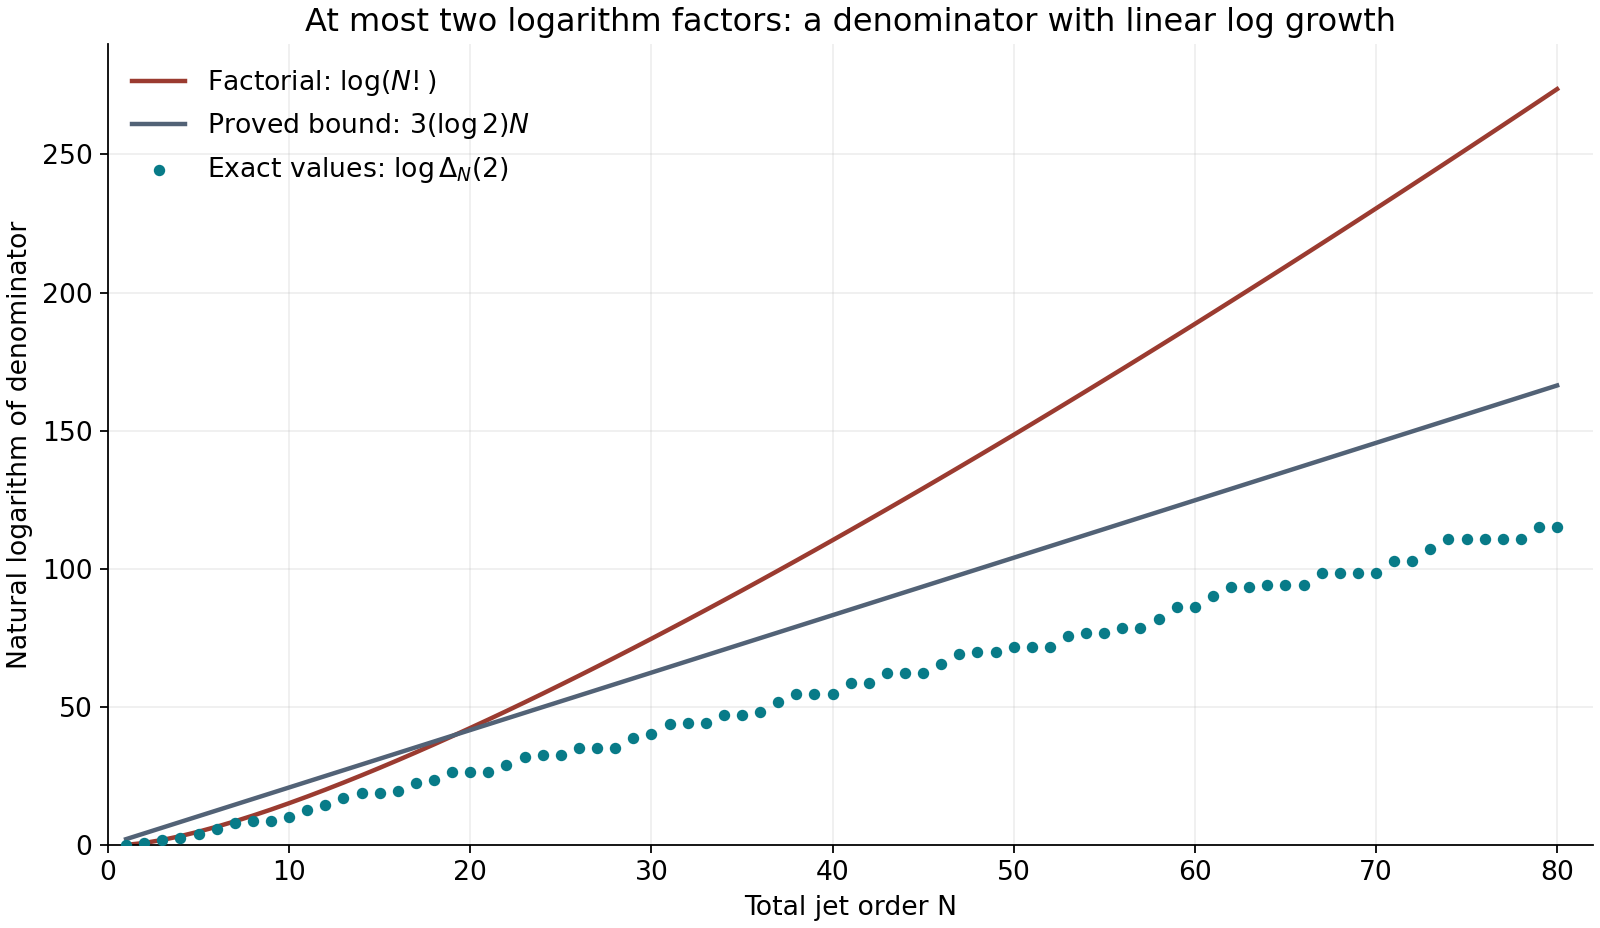
\includegraphics[keepaspectratio,alt={Exact bounded-product denominators, a proved linear upper bound, and the factorial denominator for comparison.}]{../verification/lesson22/first-jet-denominators.png}}
\par\smallskip
\begin{flushleft}\small
\emph{Figure 22.11. For integer orders \(1\le N\le80\), the lower dots
give \(\log\Delta_N(2)\) exactly; the straight line is the bound
\(3(\log2)N\) from Lemma 22.137. The other curve gives \(\log(N!)\). The
denominator \(\Delta_N(2)\) clears products from at most two logarithm
factors. The additive degree, rather than the derivative order, bounds
that number of factors in (22.457). The plotted values illustrate the
proved estimate; they do not prove it.}
\end{flushleft}
\end{minipage}\par\medskip


The translation to an identity-centered first jet and the use of formal
logarithms are treated in É. Gaudron,
\href{https://lmbp.uca.fr/~gaudron/art4.pdf}{\emph{Mesures
d'indépendance linéaire de logarithmes dans un groupe algébrique
commutatif}}, Sections 6.11--6.13. The bounds above give these steps for
the stated plane cubic models and specify the homogeneous normalization
used by the analytic function.

\subsection{A quantitative estimate with fixed elliptic
data}\label{a-quantitative-estimate-with-fixed-elliptic-data}

Fix \(E_1,\ldots,E_g\), algebraic points \(p_i\), and logarithms \(u_i\)
in the normalization of Proposition 22.136. Fix a number field \(K\)
containing the curve equations, the points and the addition tuples. Fix
an integer \(D_*\ge[K:\mathbf Q]\). Constants in this section may depend
on these data and on \(D_*\), but not on the variable coefficients of
the linear form. Use the entire lifts of Proposition 22.165. Write \[
 n=g+1,\quad K_g=n!3^g,\quad
 k_g=n!2^n(3n)^g,\quad a_0=\frac{\log2}{4}.
 \tag{22.470}
\] The symbol \(K_g\) is a numerical constant; \(K\) is the fixed number
field.

Initially assume \(\beta_i\ne0\) and
\(\max(|u_0|,|\beta_1|,\ldots,|\beta_g|)\le1\). Set
\(L=K(u_0,\beta_1,\ldots,\beta_g)\), \(D_L=[L:\mathbf Q]\le D_*\),
\(H=h(1:u_0:\beta_1:\cdots:\beta_g)\), \(u=(u_0,u_1,\ldots,u_g)\),
\(p=(u_0,p_1,\ldots,p_g)\), and
\(w=(\sum_i\beta_i u_i,u_1,\ldots,u_g)\in W\). Thus \(u-w=\Lambda e_0\),
where \(\Lambda=u_0-\sum_i\beta_i u_i\).

\subsubsection{Lemma 22.169. Uniform growth and arithmetic
bookkeeping}\label{lemma-22.169.-uniform-growth-and-arithmetic-bookkeeping}

Fix \(C_0\ge2\). There are an integer \(m\ge5\), a constant
\(R_0\ge C_0^2\), and constants \(b_0,c\ge1\) with the following
properties. The constant \(c\) can be chosen independently of \(C_0\).
For an integer \(S\ge1\), put \[
 R=R_0(S+1)^m,\qquad
 d=\left\lceil\frac{(S+1)R^g}{C_0K_g}\right\rceil,
 \qquad U=A(H+1),
 \tag{22.471}
\] where \[
 A\ge C_0^2(d+1)+b_0(d+1)(1+\log(S+1)).
 \tag{22.472}
\] Suppose \(1\le D_i\le U/R\) for \(i\ge1\) and \(0\le D_0\le d\). Use
the monomial basis of Proposition 22.149, and the field basis \(\xi_j\)
of Lemma 22.142. Let \(\ell=\dim H^0(X,\mathcal L_D)\) and
\(\nu=D_L\ell\).

For every basis monomial, use its entire expression
\(M_\lambda(z)=X^\lambda(1,z_0,\Phi_1(z_1),\ldots,
\Phi_g(z_g))\). Sampling divided jets of \(\xi_jM_\lambda\) in either
basis specified below gives matrix rows with sum of moduli at most
\(e^{cU}\). Also \(\log(1+4\nu)\le cU\).

More generally, if \(|a_{\lambda j}|\le e^\delta\) and
\(F=\sum_{\lambda,j}a_{\lambda j}\xi_jM_\lambda\), then \[
 \left|D_f^\alpha F(z)/\alpha!\right|
       \le e^{\delta+cU},\qquad
 \left|\partial_0D_f^\alpha F(z)/\alpha!\right|
       \le e^{\delta+cU}.
 \tag{22.473}
\] These bounds hold for every order \(\alpha\), at \(z=\zeta w\) for
\(|\zeta|\le8(4n+2)(S+1)\), and on segments joining \(su\) to \(sw\),
\(0\le s\le2nS\). They hold for the canonical graph basis and for an
orthonormal graph basis, with or without replacing its last member by
\(w\). Independence of the replaced basis is not needed for this growth
assertion.

For integer \(a_{\lambda j}\), the first nonzero canonical jet at a
point \(sp\), \(0\le s\le nS\), of order \(N\le nU\), satisfies \[
 \log|f_\alpha|\ge-D_L\delta-C_aU(1+\log(S+1)),
 \tag{22.474}
\] for a constant \(C_a\) independent of \(S,A,H,L\). Here \(C_a\) may
depend on the already fixed \(C_0,R_0\).

\textbf{Proof.} Fix a field basis \(\theta\) of \(K\) containing one. At
the specified embedding the basis in Lemma 22.142 satisfies
\(\max_j|\xi_j|\le\Theta:=\max_j|\theta_j|\), since the generators
\(u_0,\beta_i\) have modulus at most one. All the stated directions have
coordinates bounded by a constant depending only on
\(g,u_1,\ldots,u_g\). The stated centers, their segments, and their
translates by a unit polydisc in any of these directions and in \(e_0\),
have all coordinates at most \(C(S+1)\). This follows directly from
\(|u_0|,|\beta_i|\le1\).

The two-sided lift estimate, using its upper half, bounds every monomial
on those polydiscs by \[
 \{C(S+1)\}^{d}
       \exp\left(C'(S+1)^5\sum_iD_i\right).
 \tag{22.475}
\] Choose \(m\) at least five and at least the fixed point-height
exponents in Corollary 22.166. Choose \(R_0\ge gC'\), as well as
\(R_0\ge C_0^2\). After enlarging \(b_0\), (22.472) makes the logarithm
of (22.475) at most \(2U\).

Cauchy's coefficient formula on the unit polydisc in the direction
parameters bounds every divided jet by the same supremum. Adding an
independent parameter in direction \(e_0\) bounds the mixed coefficient
with exponent one in that parameter as well. This proves the derivative
estimates for a single monomial, without an order-dependent factorial.

There are \(\nu=D_L(D_0+1)\prod_i3D_i
\le D_*(d+1)3^gU^g\) columns. Hence row sums and the function \(F\) are
bounded by \(\nu\Theta e^{2U}\) and \(\nu\Theta e^{\delta+2U}\). Since
\(\log U\le U\) for \(U\ge1\), increasing \(b_0\) absorbs
\(\log(d+1)+\log(5D_*3^g\Theta)\) into \(U\). A constant \(c\) depending
only on \(g\) and the fixed data then proves (22.473), the row bound,
and the bound for \(\log(1+4\nu)\). Larger fixed choices of \(c\)
preserve all these assertions.

For the last assertion, Lemmas 22.142 and 22.145 give \[
 D_L h_c(P)\le D_L\delta+
 D_L\log D_L+D_L h(\theta)+D_L([L:K]-1)H.
 \tag{22.476}
\] Increase \(b_0\) so that the terms after \(D_L\delta\), the term
\(D_L dH\), and the term \(D_L d\log((g+1)((g+1)S+1))\) in (22.463) are
each at most a fixed multiple of \(U\). This is possible uniformly:
\(H/U\le1/A\), \(1/U\le1/A\), and \(D_L\le D_*\), whereas (22.472)
contains both \(d+1\) and \((d+1)\log(S+1)\). The elliptic point term in
(22.463) is at most \(CgU/R_0\). The monomial count contributes at most
\(D_L\log((d+1)3^gU^g)\). Finally \[
 \log(d+1)\le C''+(mg+1)\log(S+1),\qquad
 H_d\le1+\log(d+1).
 \tag{22.477}
\] The first bound follows from the ceiling in (22.471). Insert these
estimates and \(N\le nU\) into (22.463). All remaining terms are bounded
by \(C_aU(1+\log(S+1))\). This proves (22.474) with \(C_a\) independent
of the choices made after \(C_0,R_0\). \(\square\)

\subsubsection{Lemma 22.170. A uniformly controlled sampling
basis}\label{lemma-22.170.-a-uniformly-controlled-sampling-basis}

Assume the hypotheses of Lemma 22.151 with
\(\widetilde D=(d,U/R,\ldots,U/R)\) from (22.471), and let \(B_*\) be
its minimizing subgroup. Throughout the remainder of this section use
\(t=x\widetilde D\) and \(D_i=\lfloor t_i\rfloor\) supplied by that
lemma. These hypotheses hold if \(C_0\ge4K_g\) and (22.472) holds.
Indeed \(Q_{\{0\}}\le S+1\), so the last inequality in (22.411) is
precisely \(Q_{\{0\}}R^g/(C_0K_gd)\le1\).

There are constants \(b_1\ge1\), \(J\ge1\), independent of \(S,A,H,L\),
such that the following dichotomy holds when \(\Lambda\ne0\).

If no \(sp\), \(1\le s\le2nS\), belongs to \(\{0\}\times B_*\), then
\(Q_{B_*}=S+1\), and use an orthonormal graph basis \(f\) of \(W\).
Otherwise, provided \[
 |\Lambda|<b_1^{-1}(S+1)^{-J},
 \tag{22.478}
\] there is a basis \(f=(e'_1,\ldots,e'_{g-1},w)\) as in Corollary
22.155, whose first \(\dim B_*\) members span \(\operatorname{Lie}B_*\).
In both cases conversion from \(f\)-jets of order \(N\) to canonical
graph jets costs at most \(K_S^N\), where \[
 K_S=b_1(S+1)^J.
 \tag{22.479}
\]

\textbf{Proof.} In the first case, equality of two cosets with indices
between zero and \(S\) would give a forbidden positive multiple of \(p\)
in the subgroup. The orthonormal change costs at most \(g^{3N/2}\), by
Lemma 22.143.

In the second case write \(h=\dim B_*\le g-1\). The refined bound
(22.430) gives \(\deg B_*\le C_0K_gdR^{h-g}\le C_0K_gd\). The ceiling
formula for \(d\) bounds this by \(C_1(S+1)^{mg+1}\). Equation (22.429)
therefore gives \(\operatorname{dist}(u,\operatorname{Lie}B_*)
\ge C_2(S+1)^{-(mg+2)}\), with \(C_2>0\). Choose \(J\ge mg+2\) and
\(b_1\) sufficiently large. Then (22.478) makes \(|\Lambda|\) smaller
than half this distance. Equations (22.381)--(22.382) bound the inverse
basis entry sum by \(C_3(S+1)^J\), because
\(\sum|w_i|\le\sqrt g(\sum|u_i|^2)^{1/2}\). Include the
orthonormal-to-canonical conversion by enlarging \(b_1\) once more, and
apply (22.378). The forward basis remains bounded as required in Lemma
22.169. \(\square\)

\subsubsection{Lemma 22.171. An auxiliary polynomial with small sampled
jets}\label{lemma-22.171.-an-auxiliary-polynomial-with-small-sampled-jets}

Assume \[
 C_0\ge\max\{4K_g,8k_g,2^{2n}(n-1)!\},\qquad
 X=\frac{S+1}{C_0^2}\ge4,
 \tag{22.480}
\] and use Lemma 22.170. Put \[
 T=\lfloor U\rfloor,\quad S_0=\lfloor X\rfloor,
 \quad T_0=\lfloor U/C_0^2\rfloor,\quad
 L_0=\log(576nC_0^2),\quad b=2n+1.
 \tag{22.481}
\] Fix a constant \(c\) as in Lemma 22.169, enlarged if necessary as
specified in the next lemma, and set \[
 p_*=4bL_0X+4c,\qquad
 \delta=\frac{4k_g}{D_L C_0}(p_*+2c)U.
 \tag{22.482}
\] There is a nonzero section \(P\), with integer coefficients
\(a_{\lambda j}\) in its field-basis expression,
\(|a_{\lambda j}|\le e^\delta\), such that the following sampled divided
jets have modulus at most \(e^{-p_*U}\):

\begin{itemize}
\tightlist
\item
  in the first case of Lemma 22.170, all \(f\)-jets of total order at
  most \(2nT\) at \(su\), \(0\le s<S_0\);
\item
  in the second case, all \(f\)-jets of total order at most \(2nT\) with
  last exponent less than \(T_0\), at \(su\), \(0\le s\le2nS\).
\end{itemize}

\textbf{Proof.} Both are the systems of Corollary 22.152. Multiplication
of a column by \(\xi_j\) does not increase the complex rank, so their
matrix has rank \(\rho\) satisfying \[
 \frac\rho\nu\le\frac{k_g}{D_L C_0}=:\vartheta\le\frac18.
 \tag{22.483}
\] Here \(\ell=(D_0+1)\prod_i3D_i\ge
\mathcal H_G(D)/n!\), and \(\nu=D_L\ell\). Entire frames do not change
the rank bound: the prescribed exponent sets are closed under decreasing
any exponent, so multiplication by a local unit is an invertible
triangular operation on the jet values.

For \(\rho>0\), the logarithm of the left side of (22.386), with its
\(p=p_*U\) and \(m=cU\), is at most \(2\rho\{\delta+(p_*+2c)U\}\). We
used \(\log(1+4\rho)\le\log(1+4\nu)\le cU\). The inequality
\(2\rho/(\nu-2\rho)\le4\vartheta\) and (22.482) make this at most
\(\nu\delta\). Lemmas 22.144--22.145 give the required nonzero integer
vector and section. For \(\rho=0\), a coordinate unit vector suffices.
The coefficient and field-basis height bounds of Lemma 22.169 apply in
either case. \(\square\)

\subsubsection{Lemma 22.172. Analytic continuation in both sampling
cases}\label{lemma-22.172.-analytic-continuation-in-both-sampling-cases}

There is a constant \(L_*\), depending on the fixed choices through
\(S\), but independent of \(H,L\), such that the assumption
\(0<|\Lambda|<e^{-L_*U}\) ensures (22.478) and the following bound for
every canonical divided jet of total order at most \(nT\), at \(su\),
\(0\le s\le nS\): \[
 |\text{jet}|\le K_S^{nT}
 \left\{2e^{\delta+cU-a_0XU}
              +e^{-p_*U+cU+bL_0XU}\right\}+e^{-p_*U}.
 \tag{22.484}
\] The constant \(c\) can be fixed before \(C_0,S\).

\textbf{Proof.} The fundamental theorem of calculus along the segment
from \(sw\) to \(su\), applied to (22.473), bounds the difference of any
stated divided jet by \(s|\Lambda|e^{\delta+cU}\). Since
\(\delta/U\le4k_g(p_*+2c)/C_0\), choose \(L_*\) large enough that \[
\begin{split}
 L_*&\ge p_*+4k_g(p_*+2c)/C_0+c
                         +\log(2n(S+1))+1,\\
 L_*&\ge\log b_1+J\log(S+1)+1.
\end{split}
\tag{22.485}
\] These inequalities work for all \(U\ge1\). Every sampled jet at
\(sw\) then has modulus at most \(2e^{-p_*U}\), and conversion back at
the end costs at most \(e^{-p_*U}\), in the canonical directions.

In the first case, fix \(|\alpha|\le nT\) and put
\(G_\alpha(z)=D_f^\alpha F(zw)/\alpha!\). Write \(w=\sum_jw_jf_j\). For
\(0\le m<T\), \[
 \frac{G_\alpha^{(m)}(s)}{m!}
  =\sum_{|\gamma|=m}w^\gamma
       \binom{\alpha+\gamma}{\alpha}
       \frac{D_f^{\alpha+\gamma}F(sw)}{(\alpha+\gamma)!}.
 \tag{22.486}
\] The total order on the right is at most \((n+1)T\le2nT\). Its
coefficient sum is at most \(2^{|\alpha|+m}\max(1,\sum|w_j|)^m\),
because \(\binom{\alpha+\gamma}{\alpha}\le2^{|\alpha|+m}\) and the
multinomial expansion dominates \(\sum_{|\gamma|=m}|w^\gamma|\). The sum
\(\sum|w_j|\le\sqrt g\,|w|\) is bounded by the fixed logarithms. Enlarge
the fixed \(c\) to absorb this factor and the preceding factor two. Thus
the \(S_0\) sampled one-variable jets are bounded by \(e^{-p_*U+cU}\).

Apply Lemma 22.146 with \(r=2n(S+1)\) and outer radius \(8r\). The norm
term is bounded by \(e^{\delta+cU}\), by (22.473). Since \(S_0\ge X/2\),
\(T\ge U/2\), and \(144r/S_0\le576nC_0^2\), its conclusion gives \[
 |G_\alpha(z)|\le
 2e^{\delta+cU-a_0XU}
             +e^{-p_*U+cU+L_0XU}
 \quad(|z|\le2r).
 \tag{22.487}
\] In particular it bounds all required \(f\)-jets at \(sw\),
\(0\le s\le nS\). This includes \(w=0\); formula (22.486) then has zero
terms for \(m>0\).

In the second case write \(f=(f',w)\). For a multi-index \(\alpha'\) of
length \(g-1\), \(|\alpha'|\le nT\), put
\(G_{\alpha'}(z)=D_{f'}^{\alpha'}F(zw)/\alpha'!\). Its divided
derivative of order \(m<T_0\) is exactly the sampled jet with exponents
\((\alpha',m)\). The total order is at most \(nT+T_0\le2nT\), since
\(T_0\le T\). Take \(S_1=2nS+1\), \(r=2S_1\), and outer radius \(8r\) in
Lemma 22.146. Here \(T_0\ge U/(2C_0^2)\), so \(S_1T_0\ge XU/2\); also
\(S_1T_0\le bXU\) and \(144r/S_1=288\le e^{L_0}\). Consequently the same
bound as the braces in (22.484) holds for \(G_{\alpha'}\) throughout
\(|z|\le2r\). For every \(s\le nS\), its closed unit circle about \(s\)
lies in that disc. Cauchy's formula bounds \(G_{\alpha'}^{(j)}(s)/j!\)
by that supremum for every \(j\), including \(|\alpha'|+j\le nT\). These
are precisely all the remaining \(f\)-jets. This also covers \(g=1\),
when \(\alpha'\) is empty.

Finally use Lemma 22.170 to convert the \(f\)-jets to canonical graph
jets at \(sw\). The conversion cost is at most \(K_S^{nT}\), since
\(K_S\ge1\). Apply the earlier segment estimate in the canonical
directions to return to \(su\). This proves (22.484). \(\square\)

\begin{minipage}[t]{\linewidth}
\centering
\pandocbounded{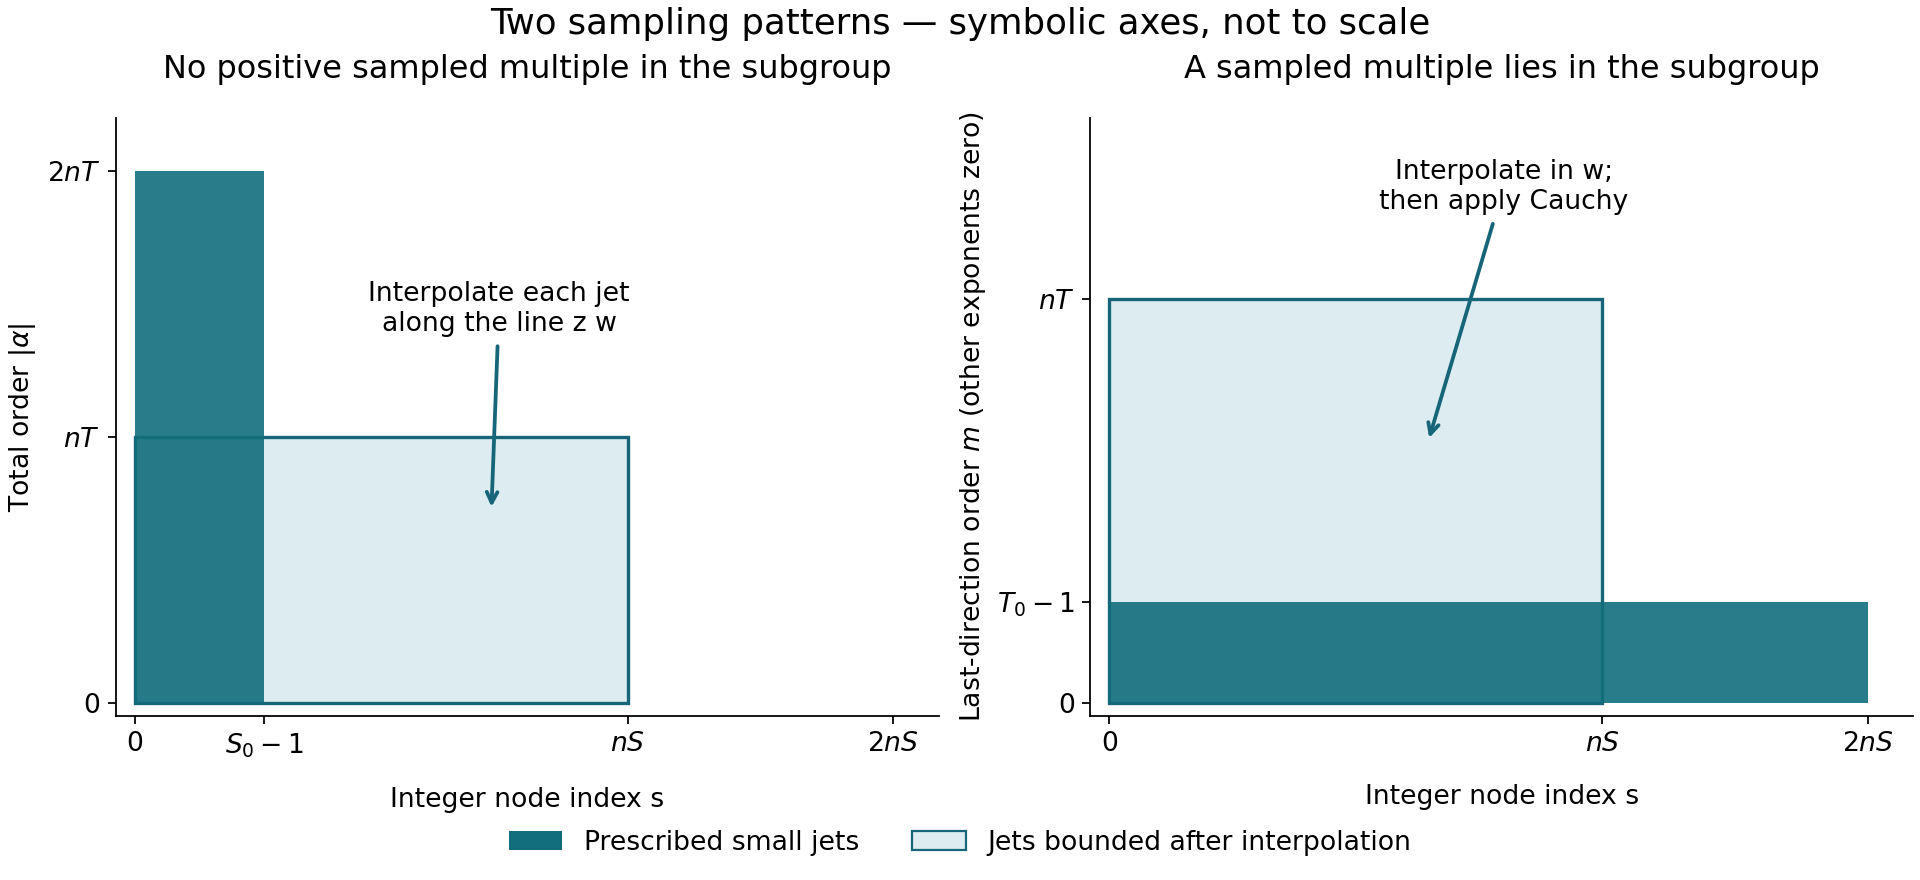
\includegraphics[keepaspectratio,alt={The two sets of prescribed small jets and the jets bounded after interpolation.}]{../verification/lesson22/elliptic-sampling-patterns.png}}
\par\smallskip
\begin{flushleft}\small
\emph{Figure 22.12. Rectangles indicate sets of integer indices; the
symbolic axes are not to scale. On the left, no positive multiple
\(sp\), \(s\le2nS\), lies in the minimizing subgroup. Few nodes carry
every jet through order \(2nT\). On the right, many nodes carry only low
orders in the last direction \(w\); the panel fixes all other exponents
at zero. The proof of Lemma 22.172 uses every \(|\alpha'|\le nT\),
recovering last orders through \(nT-|\alpha'|\) by Cauchy's formula.
Both arguments bound all required jets at the target nodes
\(0\le s\le nS\).}
\end{flushleft}
\end{minipage}\par\medskip


\subsubsection{Theorem 22.173. A fixed-data coefficient-height
estimate}\label{theorem-22.173.-a-fixed-data-coefficient-height-estimate}

For the fixed elliptic curves, algebraic points, logarithms and degree
bound above, there is \(C>0\) such that every algebraic tuple with
\([K(u_0,\beta_1,\ldots,\beta_g):\mathbf Q]\le D_*\) and
\(\Lambda=u_0-\sum_i\beta_i u_i\ne0\) satisfies \[
 \log|\Lambda|\ge
          -C\{h(1:u_0:\beta_1:\cdots:\beta_g)+1\}.
 \tag{22.488}
\] The constant may depend on the fixed logarithms and their points. The
assertion is not a numerical bound uniform in varying elliptic curves or
varying points.

\textbf{Proof.} First retain the normalization and nonzero \(\beta_i\)
used above. Fix the common constant \(c\) in Lemmas 22.169 and 22.172.
Choose \(C_0\) satisfying (22.480) and \[
 \frac{16k_gb\log(576nC_0^2)}{C_0}\le\frac{a_0}{16}.
 \tag{22.489}
\] Such a choice exists since \(\log C_0/C_0\to0\). Now fix
\(R_0,m,b_0,C_a,b_1,J\) from Lemmas 22.169--22.170. Choose the integer
\(S\) so large that \(X=(S+1)/C_0^2\ge4\) and \[
 \frac{24k_gc}{C_0}\le\frac{a_0X}{16},\qquad
 c+n\log K_S+C_a(1+\log(S+1))+\log4
                              \le\frac{a_0X}{8}.
 \tag{22.490}
\] The left side of the second inequality grows at most logarithmically
in \(S\), whereas its right side grows linearly. This proves existence.
These limiting comparisons need no unproved rate assertion:
\(\log t=\int_1^t dx/x\le2\sqrt t\) for \(t\ge1\) already suffices.
Finally define \(d,R\), choose a fixed \(A\) satisfying (22.472), and
set \(U=A(H+1)\). Every choice before \(U\) is independent of the
variable coefficient tuple and of \(H\).

Apply Lemma 22.151 to obtain the positive integer degrees \(D_i\). Its
subgroup may depend on the coefficient tuple, but all estimates in Lemma
22.170 are uniform. Fix \(L_*\) by (22.485). Suppose, for a
contradiction, that \(0<|\Lambda|<e^{-L_*U}\). The dichotomy supplies
the appropriate basis, and Lemma 22.171 supplies a nonzero auxiliary
section. By (22.482), (22.489) and the first part of (22.490), \[
 \frac{D_L\delta}{U}
   =\frac{16k_gbL_0}{C_0}X+\frac{24k_gc}{C_0}
   \le\frac{a_0X}{8}.
 \tag{22.491}
\]

Corollary 22.161 supplies a nonzero canonical jet at some \(sp\),
\(0\le s\le nS\), of order at most \(nT\). At that point take its least
nonzero total order and a nonzero coefficient \(f_\alpha\) of that
order. Entire frames preserve the order of a section, so Lemma 22.169
applies to this very coefficient. Equations (22.474), (22.490) and
(22.491) give \[
 |f_\alpha|\ge e^{-a_0XU/4}.
 \tag{22.492}
\]

On the other hand, \(T\le U\), \(\delta\le D_L\delta\), and the second
inequality in (22.490) bound the first term of (22.484) by
\(2e^{-3a_0XU/4}\). Its second term is at most \(e^{-(3bL_0-a_0/8)XU}\),
using \(p_*=4bL_0X+4c\). Since \(bL_0\ge a_0\), this is at most
\(e^{-23a_0XU/8}\). The last term is at most \(e^{-4a_0XU}\). Their sum
is at most \(4e^{-3a_0XU/4}\). Since (22.490) also gives
\(\log4\le a_0X/8\) and \(U\ge1\), \[
 |f_\alpha|\le e^{-5a_0XU/8}<e^{-a_0XU/4},
 \tag{22.493}
\] contradicting (22.492). Thus the normalized form satisfies
\(\log|\Lambda|\ge-L_*A(H+1)\).

For an arbitrary tuple, omit its zero \(\beta_i\). If none remain, Lemma
22.47 gives the assertion directly. Otherwise normalize by Lemma 22.141.
The normalized height is at most the original one, and the normalization
scalar has logarithm at least \(-D_*H\). Add this loss to the preceding
estimate. There are finitely many nonempty subsets of the fixed elliptic
factors; take the maximum of their constants and \(D_*\). This proves
(22.488) for every tuple. \(\square\)

\subsubsection{Exercise 22.174. Rational approximation to a real
elliptic
period}\label{exercise-22.174.-rational-approximation-to-a-real-elliptic-period}

Let \(\omega>0\) be a nonzero real period of \(y^2=x^3-x\) for
\(dx/(2y)\). Show that there are constants \(c_\omega>0\) and
\(\mu_\omega>0\) such that \[
 \left|\omega-\frac ab\right|
       \ge c_\omega |b|^{-\mu_\omega}
       \qquad(a,b\in\mathbf Z,\ b\ne0).
 \tag{22.494}
\] No explicit numerical value of \(\mu_\omega\) is asserted.

\textbf{Solution.} The transcendence of the nonzero period was proved in
Proposition 22.9 using Theorem 22.64, so \(a-b\omega\ne0\). Apply
Theorem 22.173 with the fixed point equal to the identity and its fixed
logarithm equal to \(\omega\). For \(B=\max(2,|a|,|b|)\), the
coefficient height is at most \(\log B\), and
\(|a-b\omega|\ge e^{-C}B^{-C}\). If \(|\omega-a/b|<1\), then
\(|a|\le(\omega+1)|b|\) and \(B\le(\omega+2)|b|\). Dividing the lower
bound by \(|b|\) proves (22.494) with \(\mu_\omega=C+1\) and
\(c_\omega=\min(1,e^{-C}(\omega+2)^{-C})\). If \(|\omega-a/b|\ge1\), the
same inequality follows from \(|b|\ge1\) and \(c_\omega\le1\).

For comparison, the freely accessible author version of É. Gaudron's
\href{https://lmbp.uca.fr/~gaudron/art4.pdf}{\emph{Mesures
d'indépendance linéaire de logarithmes dans un groupe algébrique
commutatif}}, Theorem 3 and Sections 6.6--6.13, gives a general
commutative-group estimate with the same linear coefficient-height
dependence when the group, nonadditive points, logarithms and field
degree are fixed. The proof above treats the product of the specified
plane cubic models and makes both sampling cases explicit.

\subsection{Explicit growth of elliptic homogeneous
coordinates}\label{explicit-growth-of-elliptic-homogeneous-coordinates}

Let \(\tau\) lie in the upper half-plane, put
\(y=\operatorname{Im}\tau\), and write
\(L_\tau=\mathbf Z+\tau\mathbf Z\). We use the normalization
\(\wp_\tau(z)=z^{-2}+O(z^2)\). Its construction, periodicity, Laurent
expansion and cubic equation are proved in
\href{../TR-TRANS/TR-TRANS-08.html\#1-a-lattice-and-its-weierstrass-function}{\emph{Weierstrass
functions, elliptic values and periods}, Propositions 8.1--8.2}. The
following estimates make the dependence on the lattice explicit. All
terminating decimals in the inequalities below denote exact rational
numbers.

\subsubsection{Proposition 22.175. An entire denominator and its
transformation
law}\label{proposition-22.175.-an-entire-denominator-and-its-transformation-law}

Put \(q=e^{2\pi i\tau}\), \(w=e^{2\pi iz}\), and define \[
 \phi_\tau(z)=\frac{w-1}{2\pi i}
 \prod_{r=1}^{\infty}
 \frac{(1-q^rw)(1-q^r/w)}{(1-q^r)^2}.
 \tag{22.495}
\] This is entire, has exactly the simple zeros \(L_\tau\), and
\(\phi_\tau'(0)=1\). For integers \(m,n\), \[
 \begin{split}
 \phi_\tau(z+m+n\tau)&=A_n(z)\phi_\tau(z),\\
 A_n(z)&=(-1)^n
  \exp\{-2\pi inz-\pi in(n-1)\tau\},\\
 \phi_\tau(-z)&=-e^{-2\pi iz}\phi_\tau(z).
 \end{split}
 \tag{22.496}
\]

\textbf{Proof.} On any compact set of \(z\)'s, both \(|w|\) and
\(|w|^{-1}\) are bounded. The sum of the deviations of the product
factors from one is consequently bounded by a constant times
\(\sum_r|q|^r\). For a tail with deviations at most \(1/2\), the power
series for \(\log(1+u)\) converges uniformly and absolutely. Its sum
exponentiates to a holomorphic, nowhere-zero tail product. The finitely
many other factors show normal convergence, holomorphy and the asserted
zeros. Each zero belongs to exactly one numerator factor or to \(w-1\);
that factor has a simple zero. At zero all product factors equal one,
and \((w-1)/(2\pi i)=z+O(z^2)\).

Period one is immediate. Substituting \(qw\) for \(w\) and shifting the
indices in the two numerator products gives
\(\phi_\tau(z+\tau)=-w^{-1}\phi_\tau(z)\). The identity initially holds
away from the zeros and extends across them by continuity. Iteration
gives (22.496) for positive \(n\); solving the same identity backwards
gives it for negative \(n\). Replacing \(w\) by \(w^{-1}\) interchanges
the two products and multiplies their prefactor by \(-w^{-1}\). This
proves the reflection formula. \(\square\)

\subsubsection{Proposition 22.176. Fourier and half-period
identities}\label{proposition-22.176.-fourier-and-half-period-identities}

Away from \(L_\tau\), the normally convergent expression \[
 \wp_\tau(z)=-4\pi^2\left\{
 \frac1{12}+\frac{w}{(w-1)^2}
 +\sum_{r\ge1}\left[
 \frac{wq^r}{(1-wq^r)^2}
 +\frac{w^{-1}q^r}{(1-w^{-1}q^r)^2}
 -\frac{2q^r}{(1-q^r)^2}\right]\right\}
 \tag{22.497}
\] holds. For \(v\notin L_\tau\), \[
 \frac{\phi_\tau(z+v)\phi_\tau(z-v)}{\phi_\tau(z)^2}
 =e^{-2\pi iv}\phi_\tau(v)^2
       \bigl(\wp_\tau(v)-\wp_\tau(z)\bigr).
 \tag{22.498}
\] In particular, with \(e_1=\wp_\tau(1/2)\) and
\(G(z)=\phi_\tau(z+1/2)\phi_\tau(z-1/2)/\phi_\tau(1/2)^2\), \[
 \phi_\tau^2\wp_\tau=e_1\phi_\tau^2+G,
 \qquad
 \phi_\tau^3\wp_\tau'=\phi_\tau G'-2\phi_\tau'G.
 \tag{22.499}
\] The products on the left extend holomorphically across the lattice.

\textbf{Proof.} Logarithmic differentiation of (22.495) is valid on
compact sets away from its zeros: the differentiated tails are still
bounded by a convergent geometric series. The meromorphic function
\(F=-(\phi_\tau'/\phi_\tau)'\) is periodic by (22.496). At every simple
zero of \(\phi_\tau\) it has principal part \((z-\lambda)^{-2}\), with
no simple-pole term. Thus \(F-\wp_\tau\) is entire and periodic, hence
constant. Indeed, it is bounded on a closed fundamental parallelogram
and therefore on the plane; Cauchy's derivative estimate on circles of
radius tending to infinity makes its derivative zero.

The differentiated product gives the expression in braces in (22.497)
without its constant \(1/12\) and without the last summand
\(-2q^r/(1-q^r)^2\). Since \[
 \frac{w}{(w-1)^2}
 =-\frac1{4\sin^2(\pi z)}
 =-\frac1{4\pi^2z^2}-\frac1{12}+O(z^2),
 \tag{22.500}
\] the constant Laurent coefficient of \(F\) is
\(\pi^2/3-8\pi^2\sum_{r\ge1}q^r/(1-q^r)^2\). Subtracting it yields
(22.497), because the constant coefficient of \(\wp_\tau\) is zero.

The left side of (22.498) is periodic by the transformation law and even
by the reflection formula. Its only possible poles are double poles at
the lattice, and the coefficient at zero is \(\phi_\tau(v)\phi_\tau(-v)
=-e^{-2\pi iv}\phi_\tau(v)^2\). Evenness excludes a simple-pole term.
Subtract the right side of (22.498). All poles cancel, so the difference
is constant. Its value at \(z=v\) is zero. This proves the identity. For
\(v=1/2\), \(e^{-2\pi iv}=-1\), which gives the first formula (22.499).
Differentiate it and multiply by \(\phi_\tau\); the terms containing
\(e_1\) cancel and give the second. The pole orders of \(\wp\) and
\(\wp'\) are two and three, so the stated products are entire.
\(\square\)

\subsubsection{Lemma 22.177. Rational bounds for the numerical
constants}\label{lemma-22.177.-rational-bounds-for-the-numerical-constants}

Suppose \(y\ge\sqrt3/2\), and put \(Q=e^{-2\pi y}\). Then \[
 Q<\frac1{230},\qquad
 \sqrt Q<\frac{33}{500},\qquad
 e^{-\pi y/4}<\frac{507}{1000}.
 \tag{22.501}
\] The following bounds will be used: \[
 \begin{split}
 \frac{2Q}{(1-Q)^2}+\frac{\sqrt Q(1+Q)}{1-Q}&<\frac{19}{250},\\
 e^{19/250}&<1.079,\\
 \frac{\sqrt Q(1+Q)}{(1-Q)(1-\sqrt Q)}&<0.072.
 \end{split}
 \tag{22.502}
\]

\textbf{Proof.} Here are finite rational certificates, including the
bounds for \(\pi\) used in them. For \(0<t<1\), let
\(a_N(t)=\sum_{j=0}^N(-1)^jt^{2j+1}/(2j+1)\). Integration of the finite
geometric identity for \(1/(1+t^2)\) shows that
\(a_5(t)<\arctan t<a_4(t)\). The tangent addition formula and the fact
that both angles are in \((0,\pi/2)\) give
\(\arctan(1/2)+\arctan(1/3)=\pi/4\). Direct rational comparison
therefore gives \[
 \frac{157}{50}
 <4\{a_5(1/2)+a_5(1/3)\}<\pi
 <4\{a_4(1/2)+a_4(1/3)\}<\frac{22}{7}.
 \tag{22.503}
\] Also \((433/250)^2<3\). Put \(x=67981/12500
=(157/50)(433/250)\). With \(T_N(t)=\sum_{j=0}^Nt^j/j!\), rational
arithmetic gives \[
 T_{30}(x)>230,\quad
 T_{25}(x/2)>500/33,\quad
 T_{20}(x/8)>1000/507.
 \tag{22.504}
\] Every omitted term in the exponential series is positive, so
(22.503)--(22.504) imply (22.501). These rational tests can also be
performed without large denominators by multiplying each inequality by
the corresponding positive power of \(12500\) and by \(30!\).

The first and third expressions in (22.502) increase with both \(Q\) and
\(\sqrt Q\) in \((0,1)\). Substitution of \(1/230\) and \(33/500\) gives
the stated rational inequalities. For the exponential, put \(b=19/250\).
From the twelfth term onwards, successive term ratios are at most
\(b/13\). Hence \[
 e^b\le T_{11}(b)+\frac{b^{12}}{12!}\frac1{1-b/13}
 <\frac{1079}{1000}.
 \tag{22.505}
\] The last comparison is rational. These arguments prove strict upper
bounds, rather than decimal approximations to the constants. \(\square\)

\subsubsection{Proposition 22.178. Estimates on a fundamental
cell}\label{proposition-22.178.-estimates-on-a-fundamental-cell}

Assume \(y\ge\sqrt3/2\). For \(z_0=s+t\tau\) with \(|s|,|t|\le1/2\), set
\[
 J_\tau(z)=\frac{(\operatorname{Im}z)^2}{y}
             -\operatorname{Im}z+\frac y4,
 \qquad J_\tau(z_0)=y(t-1/2)^2.
 \tag{22.506}
\] Then \[
 \begin{split}
 |\phi_\tau(z_0)|&<0.26e^{\pi J_\tau(z_0)},\\
 |\phi_\tau'(z_0)|&<1.197e^{\pi J_\tau(z_0)},\\
 |\phi_\tau(1/2)|&>0.312,\qquad
 |\wp_\tau(1/2)|<7.3.
 \end{split}
 \tag{22.507}
\] The first two estimates also hold at \(z_0+1/2\) and \(z_0-1/2\),
with the same value of \(J_\tau\).

\textbf{Proof.} Write \(a=|e^{2\pi iz_0}|=Q^t\). Thus both \(aQ\) and
\(a^{-1}Q\) are at most \(\sqrt Q\). The absolute value of the product
part of (22.495) is at most \[
 P=\prod_{r\ge1}
 \frac{(1+aQ^r)(1+a^{-1}Q^r)}{(1-Q^r)^2}
 \le\exp\left\{\frac{2Q}{(1-Q)^2}
                 +\frac{\sqrt Q(1+Q)}{1-Q}\right\}<1.079.
 \tag{22.508}
\] Indeed, \(\log(1+u)\le u\) and \(-\log(1-u)\le u/(1-u)\) follow by
integrating their respective derivatives. Also
\(a+a^{-1}\le Q^{-1/2}+Q^{1/2}\): the even function \(Q^t+Q^{-t}\)
increases with \(|t|\). Summing the geometric majorants proves (22.508).

Differentiate the numerator factors in (22.495). The sum of the absolute
logarithmic derivatives of the product, divided by \(2\pi\), is bounded
by \[
 S=\sum_{r\ge1}\left\{
  \frac{aQ^r}{1-aQ^r}+\frac{a^{-1}Q^r}{1-a^{-1}Q^r}\right\}
 \le\frac{\sqrt Q(1+Q)}{(1-Q)(1-\sqrt Q)}<0.072.
 \tag{22.509}
\] No numerator factor vanishes in this cell: its modulus parameter is
at most \(\sqrt Q<1\). Direct differentiation of the prefactor,
including at its zeros, now yields \[
 |\phi_\tau(z_0)|<0.172(1+a),\qquad
 |\phi_\tau'(z_0)|<1.079\{a+0.072(1+a)\}.
 \tag{22.510}
\] Here \(1.079/(2\pi)<0.172\) by (22.503).

Both \[
 \begin{split}
 a e^{-\pi J_\tau(z_0)}&=e^{-\pi y(t+1/2)^2}\le1,\\
 (1+a)e^{-\pi J_\tau(z_0)}
 &=e^{-\pi y(t-1/2)^2}+e^{-\pi y(t+1/2)^2}<1.507
 \end{split}
 \tag{22.511}
\] hold: at least one of \(|t-1/2|,|t+1/2|\) is at least \(1/2\). The
other exponential is at most one, and (22.501) bounds the first by
\(0.507\). The rational inequalities \(0.172\cdot1.507<0.26\) and
\(1.079(1+0.072\cdot1.507)<1.197\) prove the first two assertions of
(22.507). Integer real translations reduce \(s\pm1/2\) to the same cell
and leave both \(J_\tau\) and \(\phi_\tau,\phi_\tau'\) unchanged.

At \(z=1/2\), formula (22.495) and the reverse triangle inequality give
\[
 |\phi_\tau(1/2)|\ge\frac1\pi
  \prod_{r\ge1}\left(\frac{1-Q^r}{1+Q^r}\right)^2
 \ge\frac1\pi e^{-4Q/(1-Q)^2}
 >\frac7{22}\left(1-\frac{920}{52441}\right)>0.312.
 \tag{22.512}
\] For the middle inequality use \(\log(1-u)-\log(1+u)\ge-2u/(1-u)\),
then sum and use \(1-Q^r\ge1-Q\). For the next one use \(e^{-v}\ge1-v\)
and (22.501),(22.503).

Finally set \(w=-1\) in (22.497). The constant part has modulus
\(2\pi^2/3\). The remaining four terms for each \(r\) have total modulus
at most \(16\pi^2Q^r/(1-Q^r)^2\). Consequently \[
 |\wp_\tau(1/2)|\le\frac{2\pi^2}{3}
       +\frac{16\pi^2Q}{(1-Q)^3}<7.3,
 \tag{22.513}
\] by substituting \(\pi<22/7\) and \(Q<1/230\). \(\square\)

\subsubsection{Theorem 22.179. A global Gaussian upper
bound}\label{theorem-22.179.-a-global-gaussian-upper-bound}

For \(y\ge\sqrt3/2\), the entire tuple \[
 \Phi_\tau(z)=
 \bigl(\phi_\tau(z)^3,\;
       \phi_\tau(z)^3\wp_\tau(z),\;
       \phi_\tau(z)^3\wp_\tau'(z)\bigr)
 \tag{22.514}
\] has no common zero and represents \([1:\wp_\tau:\wp_\tau']\). With
\(\|\cdot\|_\infty\) the maximum coordinate norm, \[
 \|\Phi_\tau(z)\|_\infty
 \le3.33\exp\left\{3\pi\left(
  \frac{(\operatorname{Im}z)^2}{y}
  -\operatorname{Im}z+\frac y4\right)\right\}.
 \tag{22.515}
\] In particular it is at most \(3.33\exp\{3\pi((\operatorname{Im}z)^2/y
 +|\operatorname{Im}z|+y/4)\}\).

For a scaled lattice \(L=\omega_1 L_\tau\), \(\omega_1\ne0\), set
\(\phi_L(z)=\omega_1\phi_\tau(z/\omega_1)\) and form
\(\Phi_L=(\phi_L^3,\phi_L^3\wp_L,\phi_L^3\wp_L')\). Then \[
 \|\Phi_L(z)\|_\infty
 \le3.33\max\{1,|\omega_1|^3\}
             e^{3\pi J_\tau(z/\omega_1)}.
 \tag{22.516}
\]

\textbf{Proof.} First work on the cell of Proposition 22.178 and
abbreviate \(J=J_\tau(z_0)\). By (22.499),(22.507), the three
coordinates have respective upper bounds \[
 \begin{split}
 0.26^3 e^{3\pi J}&<0.0176e^{3\pi J},\\
 0.26^3(7.3+0.312^{-2})e^{3\pi J}&<0.309e^{3\pi J},\\
 \frac{4\cdot0.26^2\cdot1.197}{0.312^2}e^{3\pi J}
 &=3.325e^{3\pi J}<3.33e^{3\pi J}.
 \end{split}
 \tag{22.517}
\] In the third line, \(\phi G'\) supplies two summands and \(2\phi'G\)
supplies two more, each bounded by
\(0.26^2\cdot1.197e^{3\pi J}/0.312^2\). These are finite rational
comparisons.

Every \(z\) can be written \(z=z_0+m+n\tau\) with \(z_0\) in that cell.
Periodicity of \(\wp\) and \(\wp'\) and (22.496) give the exact scalar
law \[
 \Phi_\tau(z)=A_n(z_0)^3\Phi_\tau(z_0),\qquad
 \log|A_n(z_0)|=\pi\{2n\operatorname{Im}z_0+(n^2-n)y\}.
 \tag{22.518}
\] The expression in braces plus \(J_\tau(z_0)\) is exactly
\(J_\tau(z)\). Multiplication of (22.517) by \(|A_n(z_0)|^3\) proves
(22.515) globally. At zero, \(\phi=z+O(z^2)\), \(\wp=z^{-2}+O(z^2)\) and
\(\wp'=-2z^{-3}+O(z)\); thus the tuple is \((0,0,-2)\). Its scalar
transformation law proves nonvanishing at every lattice point. Away from
the lattice its first coordinate is nonzero.

Changing variables in the defining lattice series gives
\(\wp_L(z)=\omega_1^{-2}\wp_\tau(z/\omega_1)\) and
\(\wp_L'(z)=\omega_1^{-3}\wp_\tau'(z/\omega_1)\). Thus the three
coordinates of \(\Phi_L\) are those of \(\Phi_\tau(z/\omega_1)\)
multiplied by \(\omega_1^3,\omega_1,1\), respectively. Since
\(\max\{1,|\omega_1|,|\omega_1|^3\}
=\max\{1,|\omega_1|^3\}\), (22.516) follows. \(\square\)

\begin{minipage}[t]{\linewidth}
\centering
\pandocbounded{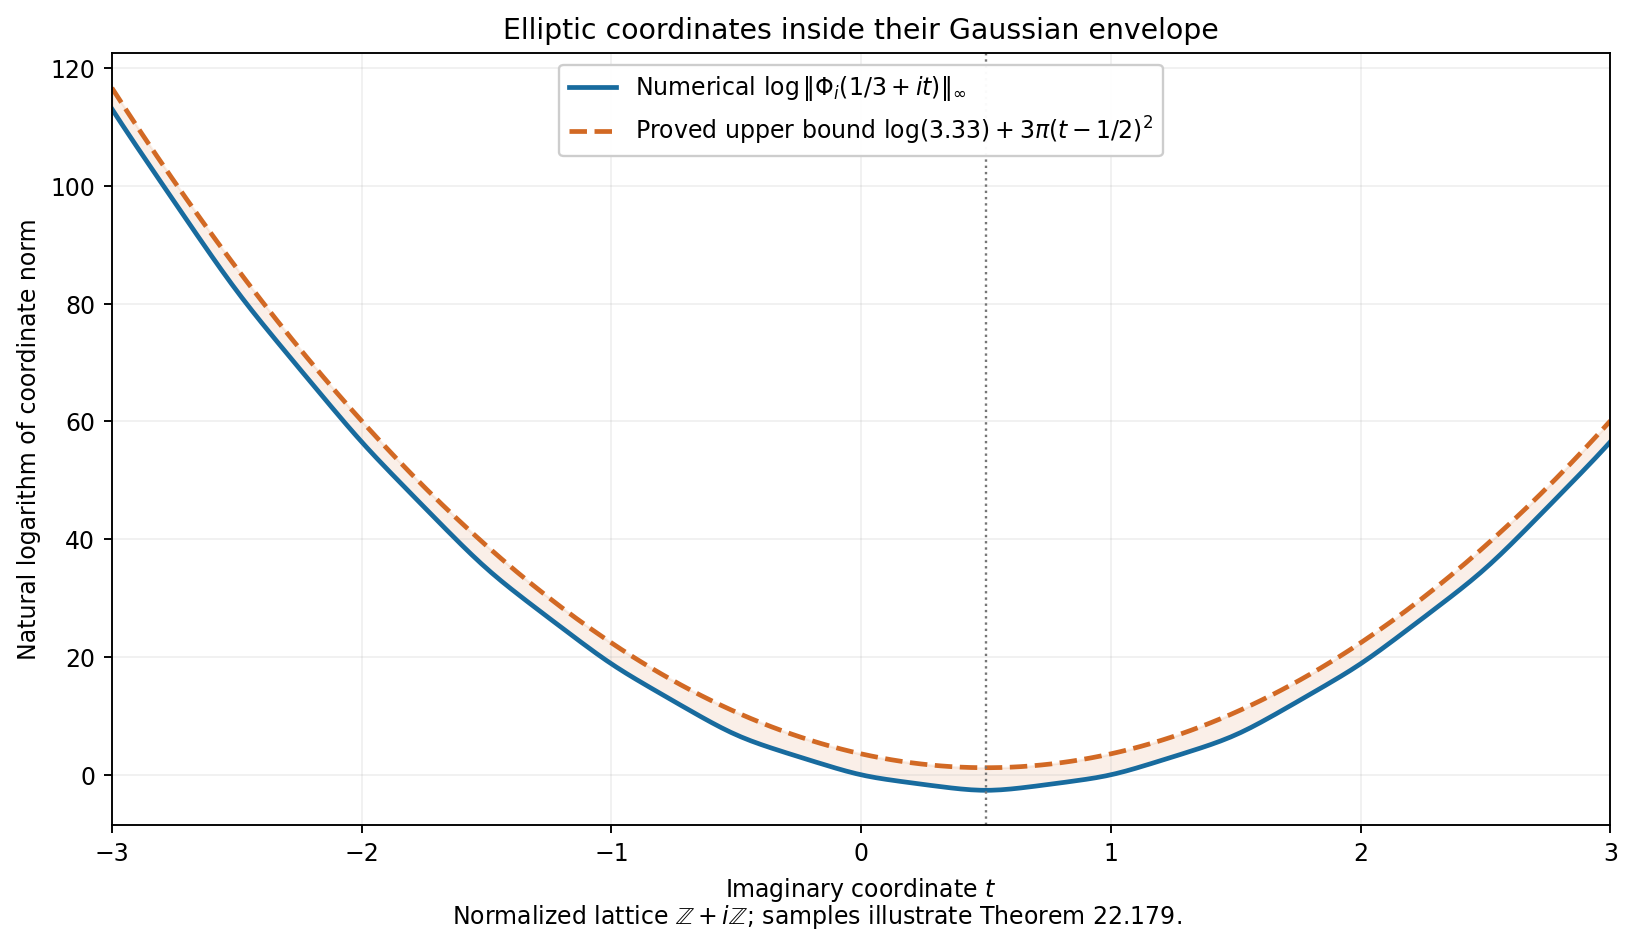
\includegraphics[keepaspectratio,alt={Elliptic homogeneous coordinates and their Gaussian upper envelope}]{../verification/lesson22/elliptic-growth-envelope.png}}
\par\smallskip
\begin{flushleft}\small
\emph{Figure 22.13. For \(\tau=i\), the blue curve shows numerically
sampled values of \(\log\|\Phi_i(1/3+it)\|_\infty\). The orange curve is
the proved upper bound \(\log(3.33)+3\pi(t-1/2)^2\). Its centre at
\(t=1/2\) comes from the chosen denominator's transformation law. The
samples illustrate (22.515); its proof is independent of them.}
\end{flushleft}
\end{minipage}\par\medskip


\subsubsection{Exercise 22.180. Differentiation and lattice
translation}\label{exercise-22.180.-differentiation-and-lattice-translation}

Find the transformation law for \(\phi_\tau'\). Explain why the estimate
for this derivative in (22.507) cannot simply be translated with the
scalar \(A_n\). For \(\tau=i\), show that there is no constant \(C\)
such that \[
 |\phi_i'(z)|\le C e^{\pi J_i(z)}\qquad(z\in\mathbf C).
 \tag{22.519}
\] Why does this not obstruct the bound for the tuple \(\Phi_i\)?

\textbf{Solution.} Differentiate (22.496): \[
 \phi_\tau'(z+m+n\tau)=
 A_n(z)\{\phi_\tau'(z)-2\pi in\phi_\tau(z)\}.
 \tag{22.520}
\] At \(z=1/3\), \(\phi_i(z)\ne0\). Dividing the absolute value of
(22.520) by \(e^{\pi J_i(z+ni)}\) gives exactly \[
 e^{-\pi/4}
 |\phi_i'(1/3)-2\pi in\phi_i(1/3)|,
 \tag{22.521}
\] which tends to infinity with \(|n|\), by the reverse triangle
inequality. This disproves (22.519) for every fixed \(C\). In contrast,
\(\wp\) and \(\wp'\) are periodic. Their products with \(\phi^3\)
therefore obey (22.518) with no derivative term. One first estimates
those complete products on a fundamental cell, then translates them.
Formula (22.499) is only needed for the cell estimate. \(\square\)

\subsubsection{Lemma 22.181. Product lower bounds on the
cell}\label{lemma-22.181.-product-lower-bounds-on-the-cell}

Keep the cell and notation of Proposition 22.178. Write \(P_\tau(z)\)
for the product in (22.495), without its prefactor. Then \[
 |P_\tau(z_0)|>0.919,\qquad
 |\phi_\tau(z_0)|\ge0.146|w-1|.
 \tag{22.522}
\] The second inequality is strict when \(w\ne1\). For
\(g(b)=b(1+b)/(1-b)^3\), one also has \[
 \begin{split}
 \sum_{r\ge1}\{|g(wq^r)|+|g(q^r/w)|\}&<\frac1{10},\\
 \frac1{12}+\sum_{r\ge1}\left\{
  \frac{aQ^r}{(1-aQ^r)^2}
  +\frac{a^{-1}Q^r}{(1-a^{-1}Q^r)^2}
  +\frac{2Q^r}{(1-Q^r)^2}\right\}&<\frac15.
 \end{split}
 \tag{22.523}
\]

\textbf{Proof.} The reverse triangle inequality and
\(\log(1-u)\ge-u/(1-u)\), \(\log(1+u)\le u\), give \[
 \log|P_\tau(z_0)|\ge
 -\frac{\sqrt Q(1+Q)}{(1-Q)(1-\sqrt Q)}
 -\frac{2Q}{1-Q}>-0.081.
 \tag{22.524}
\] The last inequality follows from (22.501)--(22.502), since
\(0.072+2/229<0.081\). Thus
\(|P_\tau(z_0)|>e^{-0.081}\ge1-0.081=0.919\). As
\(0.919\cdot7/44>0.146\), (22.503) proves (22.522).

For \(|b|\le h=\sqrt Q\), \(|g(b)|\le |b|(1+h)/(1-h)^3\). Summing
\(|wq^r|+|q^r/w|\) therefore bounds the first expression in (22.523) by
\[
 \frac{\sqrt Q(1+Q)}{1-Q}
          \frac{1+\sqrt Q}{(1-\sqrt Q)^3}<\frac1{10}.
 \tag{22.525}
\] Similarly the second expression is at most \[
 \frac1{12}
 +\frac{\sqrt Q(1+Q)}{(1-Q)(1-\sqrt Q)^2}
 +\frac{2Q}{(1-Q)^3}<\frac15.
 \tag{22.526}
\] In both cases the expressions increase with \(Q\) and \(\sqrt Q\).
Substitute \(1/230\) and \(33/500\) to obtain the displayed strict
rational inequalities. \(\square\)

\subsubsection{Theorem 22.182. An explicit lower bound for the entire
tuple}\label{theorem-22.182.-an-explicit-lower-bound-for-the-entire-tuple}

For every \(z\in\mathbf C\), \(y\ge\sqrt3/2\), \[
 \begin{split}
 \|\Phi_\tau(z)\|_\infty
 &\ge 0.073^3 e^{3\pi(J_\tau(z)-y)}\\
 &\ge 7\cdot10^{-4}
  \exp\left\{\pi\left(
  -2.51y-3|\operatorname{Im}z|
  +\frac{3(\operatorname{Im}z)^2}{y}\right)\right\}.
 \end{split}
 \tag{22.527}
\] For a scaled lattice as in Theorem 22.179, \[
 \|\Phi_L(z)\|_\infty
 \ge\min\{1,|\omega_1|^3\}\,0.073^3
       e^{3\pi(J_\tau(z/\omega_1)-y)}.
 \tag{22.528}
\]

\textbf{Proof.} First prove that the tuple norm on the cell is at least
\(c=0.073^3\). If \(|w-1|\ge1/2\), (22.522) gives
\(|\phi_\tau|\ge0.073\), so its first coordinate suffices. Suppose
instead \(|w-1|<1/2\). Differentiating (22.497) gives \[
 \phi_\tau(z_0)^3\wp_\tau'(z_0)
 =P_\tau(z_0)^3\left\{
 -w(1+w)+(w-1)^3
 \sum_{r\ge1}\bigl(g(wq^r)-g(q^r/w)\bigr)\right\}.
 \tag{22.529}
\] Multiplication removes the pole, so this identity also holds when
\(w=1\). In the present case \(|w|>1/2\) and \(|1+w|>3/2\). Lemma 22.181
gives the lower bound \(0.919^3(3/4-1/80)>0.073^3\) for the absolute
value in (22.529). This proves the cell bound, including the lattice
point.

Write \(z=z_0+m+n\tau\) as before. Since
\(J_\tau(z_0)=y(t-1/2)^2\le y\), (22.518) gives the first inequality in
(22.527). If \(v=\operatorname{Im}z\), its exponent minus the second
exponent is \(\pi\{0.26y+3(|v|-v)\}\ge0.26\pi y\). This is larger than
\(b=(13/100)(67981/12500)\), by (22.503) and \(y\ge\sqrt3/2\). The
rational comparison \(0.073^3(1+b+b^2/2)>7\cdot10^{-4}\), together with
\(e^b\ge1+b+b^2/2\), proves the second inequality. Finally the three
scaling factors from (22.516) have minimum \(\min\{1,|\omega_1|^3\}\).
This proves (22.528). \(\square\)

\subsubsection{Proposition 22.183. A lower bound for the denominator
itself}\label{proposition-22.183.-a-lower-bound-for-the-denominator-itself}

For \(z\notin L_\tau\), \(y\ge\sqrt3/2\), \[
 |\phi_\tau(z)|(1+|\wp_\tau(z)|)
 \ge0.073e^{-2\pi|\operatorname{Im}z|}
 \ge10^{-2}e^{-\pi y/2-4\pi|\operatorname{Im}z|}.
 \tag{22.530}
\] For the scaled lattice \(L=\omega_1L_\tau\) and \(z\notin L\), \[
 |\phi_L(z)|(1+|\wp_L(z)|)
 \ge\frac{0.073|\omega_1|}{\max\{1,|\omega_1|^2\}}
       e^{-2\pi|\operatorname{Im}(z/\omega_1)|}.
 \tag{22.531}
\]

\textbf{Proof.} On the cell, if \(d=|w-1|\ge1/2\), the estimate
\(|\phi_\tau|\ge0.073\) suffices. If \(0<d<1/2\), isolate the term
\(w/(w-1)^2\) in (22.497) and use (22.523). Since \(|w|>1/2\), the
reverse triangle inequality gives \[
 |\wp_\tau(z_0)|
 >4\pi^2\left(\frac1{2d^2}-\frac15\right)
 >\frac{4\pi^2\cdot0.45}{d^2}.
 \tag{22.532}
\] Multiply by \(|\phi_\tau(z_0)|>0.146d\). The resulting bound is
greater than \(8(157/50)^2\cdot0.45\cdot0.146>0.073\), because
\(d<1/2\). Thus the first product in (22.530) is at least \(0.073\)
throughout the cell away from the lattice.

For the translation \(z=z_0+m+n\tau\), set \(M/y=n^2-n+2nt\), so that
\(|A_n(z_0)|=e^{\pi M}\). If \(n\le0\), then \(M/y\ge n^2\ge0\); if
\(n\ge2\), then \(M/y\ge n(n-2)\ge0\). For \(n=0\) it is zero. The
remaining case is \(n=1\). If \(t\ge0\), again \(M\ge0\). If
\(-1/2\le t<0\), then \(M=2ty\ge-2(1+t)y=-2|\operatorname{Im}z|\). Thus
\(M\ge-2|\operatorname{Im}z|\) in every case. Periodicity of \(\wp\) and
(22.496) prove the first inequality in (22.530). The second follows from
\(0.073>0.01\) and \(y>0\). Finally \(1+|\omega_1|^2|\wp_L|\le
\max\{1,|\omega_1|^2\}(1+|\wp_L|)\), so the scaling identities prove
(22.531). \(\square\)

The three bounds (22.515), (22.527) and (22.530) include the growth
estimates of S. David,
\href{https://smf.emath.fr/system/files/filepdf/MSMF_1995_2_62__1_0.pdf}{\emph{Minorations
de formes linéaires de logarithmes elliptiques}, Proposition 3.1}. The
product identities, constants and lattice scalings above give their
proofs in the present normalization.

\subsection{Periods, curve heights and explicit derivative
bounds}\label{periods-curve-heights-and-explicit-derivative-bounds}

We use the functions and lattice normalization of Propositions
22.175--22.183. Put \(Q=|q|=e^{-2\pi y}\), where \(q=e^{2\pi i\tau}\)
and \(y=\operatorname{Im}\tau\ge\sqrt3/2\). In particular \(Q<1/230\).
Decimal constants below are exact rational numbers. The algebraic curve
convention in this section is \(Y^2=4X^3-g_2X-g_3\); its projective
coordinates are \([1:\wp:\wp']\).

\subsubsection{Proposition 22.184. Fourier expansions of the
invariants}\label{proposition-22.184.-fourier-expansions-of-the-invariants}

For \(r\ge1\), let \(\sigma_r(n)=\sum_{d\mid n}d^r\). Define \[
 E_4(q)=1+240\sum_{n\ge1}\sigma_3(n)q^n,
 \qquad
 E_6(q)=1-504\sum_{n\ge1}\sigma_5(n)q^n.
 \tag{22.533}
\] Then \[
 g_2(L_\tau)=\frac{4\pi^4}{3}E_4(q),\qquad
 g_3(L_\tau)=\frac{8\pi^6}{27}E_6(q),
 \qquad |g_2(L_\tau)|<272,\quad |g_3(L_\tau)|<1005.
 \tag{22.534}
\]

\textbf{Proof.} In a small disc around zero, expand
\(b/(1-b)^2=\sum_{m\ge1}mb^m\) in (22.497). Absolute convergence permits
both summation and differentiation. Thus \[
 \wp_\tau(z)=\frac{\pi^2}{\sin^2(\pi z)}-\frac{\pi^2}{3}
 -4\pi^2\sum_{r,m\ge1}m q^{rm}
       (e^{2\pi imz}+e^{-2\pi imz}-2).
 \tag{22.535}
\] The first term minus its constant has expansion
\(z^{-2}+\pi^4z^2/15+2\pi^6z^4/189+O(z^6)\), obtained by squaring and
inverting the sine series. The coefficients of \(z^2\) and \(z^4\) in
\(\wp\) are \(g_2/20\) and \(g_3/28\). Indeed, inserting
\(\wp=z^{-2}+az^2+bz^4+O(z^6)\) in \(\wp'^2=4\wp^3-g_2\wp-g_3\) gives
\(20a=g_2\) and \(28b=g_3\) by comparing the coefficients of \(z^{-2}\)
and one. Comparison in (22.535) gives (22.533)--(22.534), because
\(\sum_{r,m\ge1}m^j q^{rm}=\sum_n\sigma_j(n)q^n\).

Applying \(Q\,d/dQ\) repeatedly to \(Q/(1-Q)\) gives \[
 \begin{split}
 \sum_{n\ge1}\frac{n^3Q^n}{1-Q^n}
 &\le\frac{Q(1+4Q+Q^2)}{(1-Q)^5}=:S_3(Q),\\
 \sum_{n\ge1}\frac{n^5Q^n}{1-Q^n}
 &\le\frac{Q(1+26Q+66Q^2+26Q^3+Q^4)}{(1-Q)^7}=:S_5(Q).
 \end{split}
 \tag{22.536}
\] Here \((1-Q^n)^{-1}\le(1-Q)^{-1}\). The identities for
\(\sum n^jQ^n\) follow inductively by differentiation, so no divisor-sum
estimate has been omitted. Substituting \(Q=1/230\) and \(\pi<22/7\)
gives the rational bounds \[
 \frac43(22/7)^4(1+240S_3(1/230))<272,\quad
 \frac8{27}(22/7)^6(1+504S_5(1/230))<1005.
 \tag{22.537}
\] All relevant series majorants increase with \(Q\), proving the
assertions. \(\square\)

\subsubsection{Lemma 22.185. A finite discriminant
estimate}\label{lemma-22.185.-a-finite-discriminant-estimate}

For \(0<|q|\le1/230\), \[
 \left|\frac{E_4(q)^3-E_6(q)^2}{1728q}-1\right|<\frac{11}{100}.
 \tag{22.538}
\] Consequently, with \(\Delta_\tau=g_2(L_\tau)^3-27g_3(L_\tau)^2\), \[
 \frac{89}{100}(2\pi)^{12}Q
 <|\Delta_\tau|<\frac{111}{100}(2\pi)^{12}Q.
 \tag{22.539}
\]

\textbf{Proof.} We give a finite polynomial and tail calculation. The
degree-four truncations of the two series are \[
 \begin{split}
 A(q)&=1+240q+2160q^2+6720q^3+17520q^4,\\
 B(q)&=1-504q-16632q^2-122976q^3-532728q^4.
 \end{split}
 \tag{22.540}
\] For \(j>1\), \(\sigma_j(n)=n^j\sum_{d\mid n}d^{-j}
\le n^j(1+\int_1^\infty t^{-j}\,dt)
=j n^j/(j-1)\). The ratio of consecutive \(n^jQ^n\), for \(n\ge5\), is
at most \((6/5)^jQ\). Therefore, for \(|q|\le Q\le1/230\), \[
 |E_4-A|\le R_4:=\frac{360\cdot5^3Q^5}{1-(6/5)^3Q},
 \qquad
 |E_6-B|\le R_6:=\frac{630\cdot5^5Q^5}{1-(6/5)^5Q}.
 \tag{22.541}
\] Put \(A_+=1+240Q+2160Q^2+6720Q^3+17520Q^4\) and
\(B_+=1+504Q+16632Q^2+122976Q^3+532728Q^4\). Let \(d_j=[q^j](A^3-B^2)\).
Its coefficients for \(j=0,\ldots,12\) are, in that order, \[
\begin{gathered}
 0,\ 1728,\ -41472,\ 435456,\ -2543616,\ 5104512,\\
 1525813632,\ 50747641344,\ 424509633216,\\
 2050306560000,\ 4362564096000,\ 6188120064000,\ 5377771008000.
\end{gathered}
\tag{22.542}
\] It follows that the left side of (22.538) is at most \[
 \frac{\sum_{j=2}^{12}|d_j|Q^j
 +R_4(3A_+^2+3A_+R_4+R_4^2)+R_6(2B_++R_6)}{1728Q}.
 \tag{22.543}
\] Every summand after division by \(Q\) is increasing on this interval.
Substitution of \(Q=1/230\) is a rational calculation and gives a value
less than \(10924/100000<11/100\). Thus (22.538) follows. Finally
\(\Delta_\tau=(64\pi^{12}/27)(E_4^3-E_6^2)\), and
\((64/27)1728=4096=2^{12}\), giving (22.539). \(\square\)

\subsubsection{Proposition 22.186. Period bounds and the imaginary part
of the
lattice}\label{proposition-22.186.-period-bounds-and-the-imaginary-part-of-the-lattice}

Let \(L=\omega_1(\mathbf Z+\tau\mathbf Z)\), \(g_2=g_2(L)\),
\(g_3=g_3(L)\), and \(j=1728g_2^3/(g_2^3-27g_3^2)\). If \(j\ne0\), then
\[
 \frac{e^{1.825-\pi y/6}|j|^{1/12}}{(12|g_2|)^{1/4}}
 \le |\omega_1|\le
 \frac{e^{1.85-\pi y/6}|j|^{1/12}}{(12|g_2|)^{1/4}}.
 \tag{22.544}
\] Suppose now that \(g_2,g_3\) belong to a number field of degree
\(D\), at the given complex embedding, and put \[
 h_E=h(1:g_2:g_3),\qquad h=\max\{1,h_E,h(j)\}.
 \tag{22.545}
\] Then \(y\le Dh\), including when \(j=0\).

\textbf{Proof.} Lattice scaling gives \(g_2(L_\tau)=\omega_1^4g_2\) and
\(g_3(L_\tau)=\omega_1^6g_3\), either from their lattice sums or their
Laurent coefficients. Thus \(j\) is unchanged by scaling. If \(j\ne0\),
then \(g_2\ne0\), and \[
 |\omega_1|
 =\frac{|\Delta_\tau|^{1/12}|j|^{1/12}}
        {(12|g_2|)^{1/4}}.
 \tag{22.546}
\] Apply (22.539). The elementary numerical comparisons required are
\(2\pi(0.89)^{1/12}>e^{1.825}\) and \(2\pi(1.11)^{1/12}<e^{1.85}\). They
follow using \(157/50<\pi<22/7\) from (22.503): the degree-twenty
exponential sum with geometric remainder bounds \(e^{1.825}\) from
above, and its degree-twenty sum bounds \(e^{1.85}\) from below. Raising
the resulting positive rational inequalities to the twelfth power
verifies both comparisons. This proves (22.544).

To control \(y\), there is nothing to prove if \(y\le1\). If \(y>1\),
then \(Q<1/500\): the positive exponential sum
\(\sum_{r=0}^{30}(157/25)^r/r!\) is greater than \(500\), and
\(2\pi>157/25\). Equation (22.536) gives \(240S_3(1/500)<1/2\). Hence
\(|E_4|>1/2\), and (22.538) gives \[
 |j|=\left|\frac{1728E_4^3}{E_4^3-E_6^2}\right|
 >\frac{25}{222Q}=\frac{25}{222}e^{2\pi y}>e^y.
 \tag{22.547}
\] For the last inequality, \((2\pi-1)y>5\) and \(e^5>1+5+25/2>222/25\).
The chosen-embedding height bound \(\log\max\{1,|j|\}\le D h(j)\) now
gives \(y<Dh\). This also shows that \(j=0\) forces \(y<1\), so no
exceptional case has been omitted.

Every lattice admits the stipulated normalization. Choose a shortest
nonzero vector \(\omega_1\). It is primitive in a lattice basis and
therefore extends to a basis, by the integer Bézout identity. Choose the
other vector's sign to make \(y>0\), and add an integer multiple of
\(\omega_1\) so that \(|\operatorname{Re}\tau|\le1/2\). Minimality gives
\(|\tau|\ge1\), whence \(y\ge\sqrt3/2\). \(\square\)

\subsubsection{Theorem 22.187. Entire growth controlled by the curve
height}\label{theorem-22.187.-entire-growth-controlled-by-the-curve-height}

For the curve and embedding of (22.545), the entire tuple \(\Phi_L\) of
Theorem 22.179 satisfies \[
 \|\Phi_L(z)\|_\infty
 \le3.33\exp\left\{\frac34Dh_E
                    +3\pi J_\tau(z/\omega_1)\right\}.
 \tag{22.548}
\] In particular this remains valid with \(J_\tau(w)\) replaced by
\((\operatorname{Im}w)^2/y+|\operatorname{Im}w|+y/4\). The assertion
includes curves with \(g_2=0\) or \(g_3=0\).

\textbf{Proof.} The separate bounds in (22.517) transform by the same
scalar law as the tuple. They therefore give, for \(r=|\omega_1|\), \[
 \|\Phi_L(z)\|_\infty
 \le \max\{0.0176r^3,\ 0.309r,\ 3.33\}
       e^{3\pi J_\tau(z/\omega_1)}.
 \tag{22.549}
\] For a nonzero \(g_i\), the height definitions give
\(\log\max\{1,|g_i|^{-1}\}\le D h_E\): projection bounds \(h(g_i)\) by
\(h_E\), the product formula gives \(h(g_i^{-1})=h(g_i)\), and the
nonnegative contribution of the chosen archimedean place is at least
\(1/D\) times the relevant logarithm. These are the same height
identities used in Lemma 22.141.

If \(g_2\ne0\), (22.534) implies \(r^4<272e^{Dh_E}\). Thus the first two
factors in (22.549) are bounded by \(0.0176\,272^{3/4}e^{3Dh_E/4}\) and
\(0.309\,272^{1/4}e^{Dh_E/4}\), respectively. Their constant factors are
less than \(3.33\), as is checked by fourth powers. If \(g_2=0\),
nonsingularity gives \(g_3\ne0\), and \(r^6<1005e^{Dh_E}\). The
corresponding constants are \(0.0176\sqrt{1005}\) and
\(0.309\,1005^{1/6}\), again less than \(3.33\); their height exponents
are \(Dh_E/2\) and \(Dh_E/6\). Since \(h_E\ge0\), every case is bounded
by (22.548). \(\square\)

\begin{minipage}[t]{\linewidth}
\centering
\pandocbounded{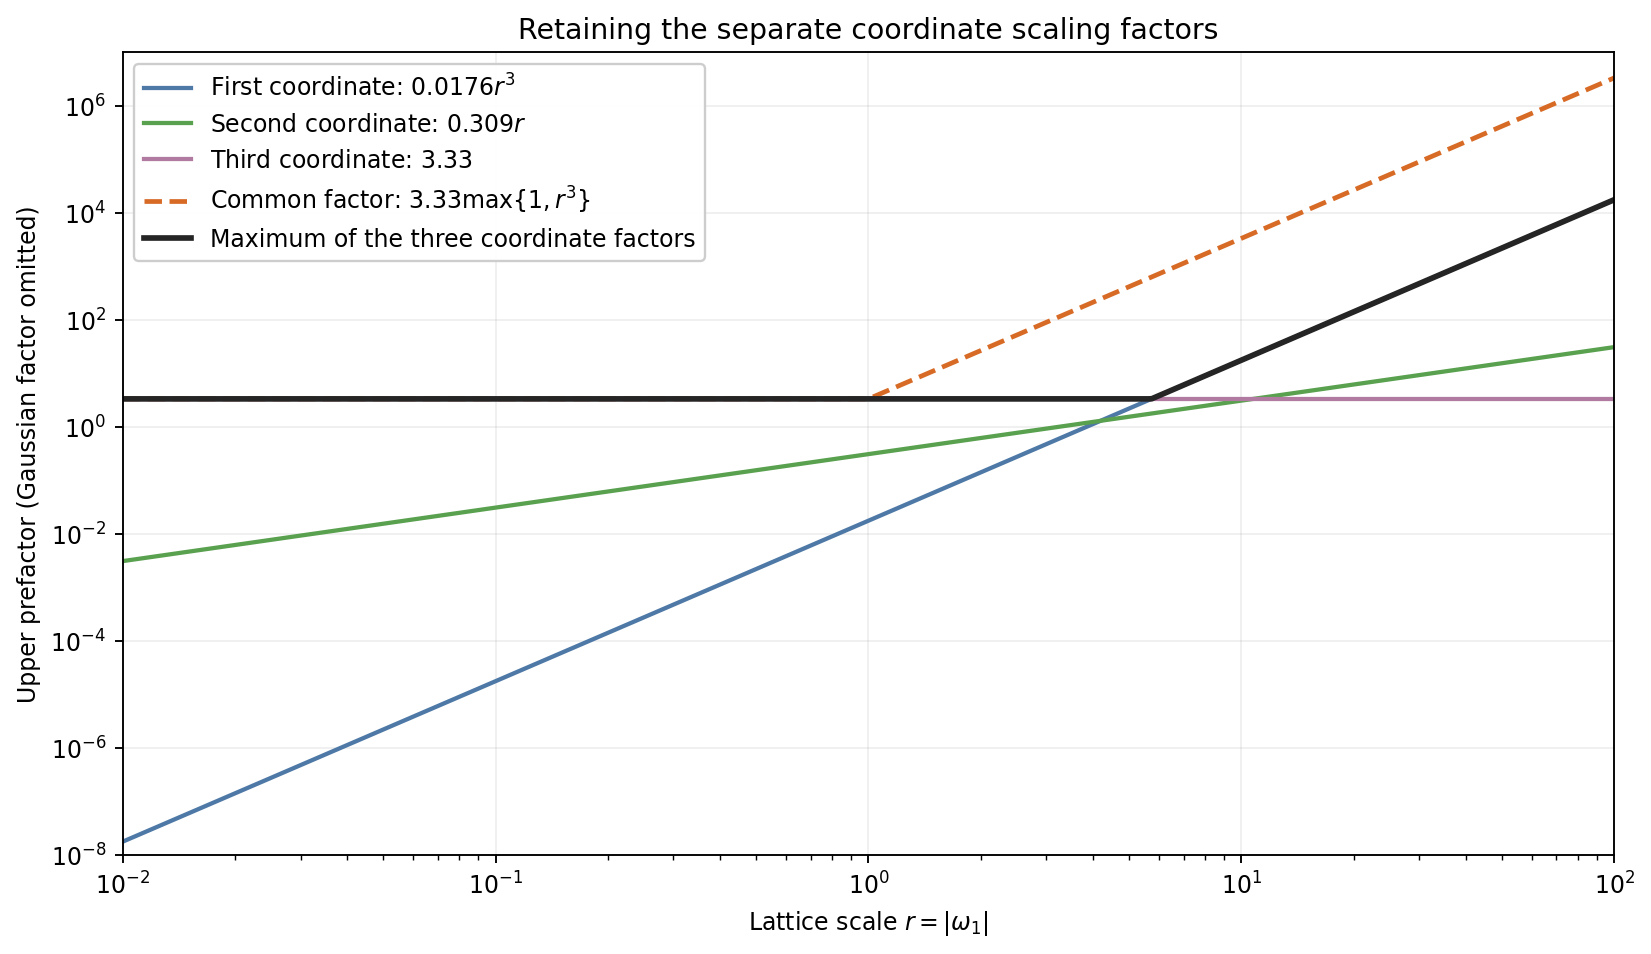
\includegraphics[keepaspectratio,alt={Separate coordinate factors under a lattice scaling}]{../verification/lesson22/elliptic-scaled-growth.png}}
\par\smallskip
\begin{flushleft}\small
\emph{Figure 22.14. Scaling the lattice by a complex number of modulus
\(r\) multiplies the three coordinate bounds by \(r^3,r,1\). The solid
black envelope in (22.549) retains these separate factors. The dashed
curve is the coarser common factor \(3.33\max\{1,r^3\}\) from (22.516).
Both are upper bounds; the curves do not plot values of an elliptic
function.}
\end{flushleft}
\end{minipage}\par\medskip


\subsubsection{Proposition 22.188. Explicit bounds for mixed directional
derivatives}\label{proposition-22.188.-explicit-bounds-for-mixed-directional-derivatives}

For \(i=1,\ldots,k\), let \(E_i\) and \(L_i=\omega_iL_{\tau_i}\) have
the preceding normalization over a common field of degree \(D\). Put
\(y_i=\operatorname{Im}\tau_i\) and \(h_i=h(1:g_{2,i}:g_{3,i})\). Let
\(P\) be a polynomial of degree at most \(d_0\) in its additive variable
and homogeneous degree \(d_i\) in the three coordinates of its \(i\)-th
elliptic block. Suppose its \(N_P\ge1\) nonzero coefficients have
modulus at most \(H_P\). Set \[
 F(z_0,\ldots,z_k)=P(z_0,\Phi_{L_1}(z_1),\ldots,\Phi_{L_k}(z_k)).
 \tag{22.550}
\] Choose directions \(x_1,\ldots,x_l\in\mathbf C^{k+1}\), nonnegative
integers \(t_1,\ldots,t_l\), and write \[
 \begin{split}
 T&=\sum_at_a,\quad M_0=\min\{d_0,T\},\\
 \xi_0&=\max\{1,|x_{a,0}|:1\le a\le l\},\\
 \xi_1&=\max\{1,|x_{a,i}|:1\le a\le l,1\le i\le k\},\\
 b_i&=|\operatorname{Im}(v_i/\omega_i)|+|\omega_i|^{-1}.
 \end{split}
 \tag{22.551}
\] With \(D_x=\sum_{i=0}^kx_i\partial/\partial z_i\), \[
 \begin{split}
 |D_{x_1}^{t_1}\cdots D_{x_l}^{t_l}F(v)|
 \le{}&N_PH_P\,T!(k+1)^T\xi_0^{M_0}\xi_1^T
 (|v_0|+1)^{d_0}\\
 &\times\exp\left\{\sum_{i=1}^kd_i
 \left[\log(3.33)+\frac34Dh_i
       +3\pi\left(\frac{b_i^2}{y_i}+b_i+\frac{y_i}{4}\right)\right]\right\}.
 \end{split}
 \tag{22.552}
\] Here \(0!=1\); the estimate includes \(T=0\).

\textbf{Proof.} On the closed unit polydisc about \(v\),
\(|z_0|\le|v_0|+1\), and \(|\operatorname{Im}(z_i/\omega_i)|\le b_i\).
Bound each monomial by (22.548) and sum over the \(N_P\) coefficients.
This gives the right side of (22.552) without its factor
\(T!(k+1)^T\xi_0^{M_0}\xi_1^T\); denote that bound by \(M\). Iterating
the one-variable Cauchy integral formula yields
\(|\partial^\alpha F(v)|\le\alpha!M\) for \(|\alpha|=T\). This follows
directly by integrating each variable on its unit circle, so the
normalization of the derivatives is specified.

Expand the \(T\) directional derivative factors one at a time. There are
\((k+1)^T\) terms before collecting equal partial derivatives. A
surviving term chooses coordinate zero at most \(d_0\) times, since
higher additive derivatives vanish. Its coefficient is at most
\(\xi_0^{M_0}\xi_1^T\), and its partial derivative is at most \(T!M\),
because \(\alpha!\le T!\). Summation proves (22.552). No estimate of
\(N_P\) by an unspecified dimension is needed. \(\square\)

\subsubsection{Exercise 22.189. The zero invariant case and height
normalization}\label{exercise-22.189.-the-zero-invariant-case-and-height-normalization}

For \(E:Y^2=4X^3-1/2\), compute \(h_E\), \(h(j)\), and the exponents of
\(r=|\omega_1|\) in its homogeneous lift. Give an explicit
height-dependent upper bound for its tuple norm. Explain why a formula
that divides by \(g_2\) cannot be used for this curve.

\textbf{Solution.} The primitive integral coordinates of \((1:0:1/2)\)
are \((2:0:1)\), so \(h_E=\log2\). The invariant \(j\) is zero and has
height zero. Scaling from \(L_\tau\) gives multipliers
\(\omega_1^3,\omega_1,1\) on the three coordinates. Since \(g_3=1/2\),
(22.534) gives \(r^6<2010\). Formula (22.549) therefore gives \[
 \|\Phi_L(z)\|_\infty
 \le\max\{0.0176\sqrt{2010},\ 0.309\,2010^{1/6},\ 3.33\}
          e^{3\pi J_\tau(z/\omega_1)}
 =3.33e^{3\pi J_\tau(z/\omega_1)}.
 \tag{22.553}
\] The equality of the constant to \(3.33\) is a finite positive-power
comparison. The general height bound (22.548) also applies and gives the
slightly larger prefactor \(3.33\,2^{3/4}\). Formula (22.544) does not
apply: both \(j\) and \(g_2\) vanish, whereas the \(g_3\)-based argument
above has a nonzero denominator. \(\square\)

\subsubsection{Lemma 22.190. A uniform estimate near the
pole}\label{lemma-22.190.-a-uniform-estimate-near-the-pole}

For \(0<|z|\le1/10\), \[
 |\wp_\tau(z)|\ge\frac{0.9}{|z|^2}.
 \tag{22.554}
\]

\textbf{Proof.} The sine series and \(|z|\le1/10\) give \[
 |\sin(\pi z)|\le\pi|z|\,
 \frac{\sinh(\pi/10)}{\pi/10}<1.02\pi|z|.
 \tag{22.555}
\] For the last inequality, put \(u=11/35>\pi/10\). The series
\(\sinh u/u\) is bounded by \(1+u^2/(6(1-u^2/20))<1.02\): after its
quadratic term, successive ratios are at most \(u^2/20\).

Now \(|w|,|w|^{-1}\le e^{\pi/5}<15/8\). The last comparison follows from
\(\pi/5<22/35\) and the degree-twenty exponential sum with geometric
remainder. Isolating the trigonometric term in (22.497), its other terms
have total modulus at most \[
 4\pi^2\left\{\frac1{12}
 +\frac{(15/4)Q}{(1-Q)(1-15Q/8)^2}
 +\frac{2Q}{(1-Q)^3}\right\}<4.3.
 \tag{22.556}
\] Substitute \(Q=1/230\) and \(\pi=22/7\) to check the rational upper
bound. Consequently \(|\wp_\tau(z)|\ge1/(1.02^2|z|^2)-4.3\). Since
\(1/1.02^2-4.3/100>0.9\), (22.554) follows. \(\square\)

The period inequalities (22.544) are the estimates in S. David,
\href{https://smf.emath.fr/system/files/filepdf/MSMF_1995_2_62__1_0.pdf}{\emph{Minorations
de formes linéaires de logarithmes elliptiques}, Lemma 3.2}. The finite
discriminant argument proves them here. Theorem 22.187 and Proposition
22.188 supply height-sensitive growth and derivative estimates with the
support size of the polynomial explicitly retained.

\subsection{Canonical heights from explicit duplication
certificates}\label{canonical-heights-from-explicit-duplication-certificates}

Let \(E/K\) be the nonsingular cubic \[
 E:\quad Y^2=4x^3-ax-b,\qquad \Delta=a^3-27b^2\ne0,
 \qquad h_E=h(1:a:b).
 \tag{22.557}
\] The absolute values and weights \(n_v/[K:\mathbf Q]\) are those of
Lemma 22.47. For a finite point put \(h_x(P)=h(1:x(P))\) and
\(h_3(P)=h(1:x(P):Y(P))\). Both heights are zero at \(O\). The subscript
three records the plane embedding associated with \(3O\).

\subsubsection{Proposition 22.191. The homogeneous duplication
map}\label{proposition-22.191.-the-homogeneous-duplication-map}

Define the binary quartics \[
 \begin{split}
 F(X,Z)&=16X^4+8aX^2Z^2+32bXZ^3+a^2Z^4,\\
 G(X,Z)&=64X^3Z-16aXZ^3-16bZ^4.
 \end{split}
 \tag{22.558}
\] They have no common projective zero. If \(x(P)=[X:Z]\), with
\(x(O)=[1:0]\), then \(x(2P)=[F(X,Z):G(X,Z)]\).

\textbf{Proof.} For \(Y(P)\ne0\), the tangent slope is
\(m=(12x^2-a)/(2Y)\). The chord law on the cubic gives
\(x(2P)=m^2/4-2x\), which is (22.558) after substituting
\(Y^2=4x^3-ax-b\). To check that the formula extends everywhere, put
\(f(x)=4x^3-ax-b\). Direct expansion gives \[
 F(x,1)=f'(x)^2-32xf(x),\qquad G(x,1)=16f(x).
 \tag{22.559}
\] A finite common zero would be a multiple root of \(f\), contrary to
\(\Delta\ne0\). At \([1:0]\), \(F=16\) and \(G=0\). Thus the displayed
pair defines a morphism on \(\mathbf P^1\). At a point with \(Y=0\) it
gives infinity, as required for a point of order two; it fixes infinity.
Equality on the remaining dense open set proves the duplication formula
everywhere. \(\square\)

\subsubsection{Lemma 22.192. Two polynomial identities with controlled
coefficients}\label{lemma-22.192.-two-polynomial-identities-with-controlled-coefficients}

For a vector \(c=(c_0,\ldots,c_7)\), write \[
 A_c=\sum_{i=0}^3c_iX^{3-i}Z^i,\qquad
 B_c=\sum_{i=0}^3c_{i+4}X^{3-i}Z^i.
 \tag{22.560}
\] The two columns of the following table define vectors \(c,d\):

{\def\LTcaptype{none} % do not increment counter
\begin{longtable}[]{@{}rll@{}}
\toprule\noalign{}
Index & \(c_i\) & \(d_i\) \\
\midrule\noalign{}
\endhead
\bottomrule\noalign{}
\endlastfoot
0 & \(256a^3-6912b^2\) & \(0\) \\
1 & \(-64a^2b\) & \(-12288\) \\
2 & \(-48a^4+1408ab^2\) & \(0\) \\
3 & \(-48a^3b+1536b^3\) & \(4096a\) \\
4 & \(16a^2b\) & \(3072\) \\
5 & \(-20a^4+512ab^2\) & \(0\) \\
6 & \(-104a^3b+3072b^3\) & \(1280a\) \\
7 & \(-3a^5+96a^2b^2\) & \(6912b\) \\
\end{longtable}
}

Then \[
 A_cF+B_cG=4096\Delta X^7,\qquad
 A_dF+B_dG=4096\Delta Z^7.
 \tag{22.561}
\] Every coefficient polynomial in this table has total degree at most
five. The sums of the absolute integer coefficients in the two columns
are \(14095\) and \(27648\), respectively.

\textbf{Proof.} Multiply (22.558) by the degree-three polynomials in
(22.560). In the first identity, the coefficient of \(X^7\) is
\(16(256a^3-6912b^2)=4096\Delta\), and the coefficients of
\(X^{7-i}Z^i\), \(1\le i\le7\), cancel. In the second, the only
surviving coefficient is that of \(Z^7\), namely
\(4096a\cdot a^2+6912b\cdot(-16b)=4096\Delta\). This proves the
identities by coefficient comparison. The degrees and column sums follow
directly from the table. \(\square\)

\subsubsection{Proposition 22.193. Explicit errors in doubling the
height}\label{proposition-22.193.-explicit-errors-in-doubling-the-height}

At an archimedean place, let \[
 U_v=\max\left\{\sum|\operatorname{coeff}(F)|_v,
                         \sum|\operatorname{coeff}(G)|_v\right\},
 \quad
 B_v=\max\left\{\sum_{i=0}^7|c_i|_v,
                         \sum_{i=0}^7|d_i|_v\right\}.
 \tag{22.562}
\] At a nonarchimedean place replace each sum by a maximum. Define \[
 U_E=\sum_v\frac{n_v}{[K:\mathbf Q]}\log U_v,
 \qquad
 B_E=\sum_v\frac{n_v}{[K:\mathbf Q]}\log B_v.
 \tag{22.563}
\] These are nonnegative, finite, and unchanged by extending \(K\). For
every \(P\in E(\overline{\mathbf Q})\), \[
 4h_x(P)-B_E\le h_x(2P)\le4h_x(P)+U_E,
 \quad
 U_E\le2h_E+\log96,\quad B_E\le5h_E+\log27648.
 \tag{22.564}
\]

\textbf{Proof.} Write \(N_v=\max\{|X|_v,|Z|_v\}\) and
\(T_v=\max\{|F(X,Z)|_v,|G(X,Z)|_v\}\). The triangle or ultrametric
inequality gives \(T_v\le U_vN_v^4\). Choose the identity (22.561) whose
right side uses a coordinate of modulus \(N_v\). Its left side has
modulus at most \(B_vN_v^3T_v\). Therefore \[
 \frac{|4096\Delta|_v}{B_v}N_v^4\le T_v\le U_vN_v^4.
 \tag{22.565}
\] Take weighted logarithms and sum. The product formula removes
\(4096\Delta\), proving the height inequalities. This cancellation is
why no inverse discriminant remains in the global error.

Set \(M_v=\max\{1,|a|_v,|b|_v\}\). At an archimedean place,
\(U_v\le96M_v^2\) and \(B_v\le27648M_v^5\), by (22.558) and the table.
At a finite place the corresponding bounds are \(M_v^2\) and \(M_v^5\),
since the table has integer coefficients. The sum of archimedean weights
is one. These facts give the last two assertions in (22.564).

Only finitely many finite places contribute to (22.563). Moreover
\(U_v\ge|16|_v\) and \(B_v\ge|3072|_v\), so their global sums are
nonnegative by the product formula. The local-degree identity under a
field extension preserves the sums, exactly as in Lemma 22.47. Thus the
inequalities hold for points over every finite extension and hence over
\(\overline{\mathbf Q}\). \(\square\)

\subsubsection{Theorem 22.194. Canonical height and a certified
convergence
interval}\label{theorem-22.194.-canonical-height-and-a-certified-convergence-interval}

The limit \[
 \widehat h_x(P)=\lim_{r\to\infty}4^{-r}h_x(2^rP)
 \tag{22.566}
\] exists, is nonnegative, and satisfies \[
 h_x(P)-B_E/3\le\widehat h_x(P)\le h_x(P)+U_E/3,
 \qquad \widehat h_x(2P)=4\widehat h_x(P).
 \tag{22.567}
\] More generally, every integer \(r\ge0\) supplies the interval \[
 4^{-r}h_x(2^rP)-\frac{B_E}{3\cdot4^r}
 \le\widehat h_x(P)\le
 4^{-r}h_x(2^rP)+\frac{U_E}{3\cdot4^r}.
 \tag{22.568}
\]

\textbf{Proof.} If \(a_r=4^{-r}h_x(2^rP)\), (22.564) gives
\(-B_E4^{-r-1}\le a_{r+1}-a_r\le U_E4^{-r-1}\). The series of absolute
differences converges, because its tail is bounded by a geometric
series. Summing that tail from \(r\) to infinity gives (22.568).
Nonnegativity follows from \(a_r\ge0\), and shifting the index in the
limit gives the doubling law. The case \(r=0\) gives (22.567).
\(\square\)

\subsubsection{Proposition 22.195. Conversion to the plane
height}\label{proposition-22.195.-conversion-to-the-plane-height}

For all \(P\in E(\overline{\mathbf Q})\), \[
 -\frac12h_E-\log2\le h_3(P)-\frac32h_x(P)
 \le\frac12h_E+\frac12\log6.
 \tag{22.569}
\] Consequently the canonical height for \(3O\) is \[
 \widehat h_3(P)=\lim_{r\to\infty}4^{-r}h_3(2^rP)
                =\frac32\widehat h_x(P),
 \tag{22.570}
\] and \[
 -C_-\le h_3(P)-\widehat h_3(P)\le C_+,
 \quad
 C_-=\frac12h_E+\log2+\frac12U_E,
 \quad
 C_+=\frac12h_E+\frac12\log6+\frac12B_E.
 \tag{22.571}
\] In particular, \[
 -\frac32h_E-\frac12\log384
 \le h_3(P)-\widehat h_3(P)
 \le3h_E+\frac12\log165888.
 \tag{22.572}
\]

\textbf{Proof.} At a finite point put \(u_v=\max\{1,|x|_v\}\),
\(v_v=\max\{1,|x|_v,|Y|_v\}\), and use \(M_v\) from Proposition 22.193.
The curve equation gives \(v_v\le\sqrt6\,M_v^{1/2}u_v^{3/2}\) at an
archimedean place and \(v_v\le M_v^{1/2}u_v^{3/2}\) at a finite place.
Indeed, the three terms \(4x^3,-ax,-b\) have total absolute value at
most \(6M_vu_v^3\) in the first case and maximum at most \(M_vu_v^3\) in
the second. Also \(u_v\le u_v^{3/2}\).

For the opposite inequality there is nothing to prove if \(u_v=1\).
Otherwise write \(4x^3=Y^2+ax+b\). At an archimedean place,
\(4u_v^3\le3M_vv_v^2\), and hence \(u_v^3\le M_vv_v^2\). At a finite
place, \(u_v^3\le |4|_v^{-1}M_vv_v^2\). The same inequalities hold when
\(u_v=1\), since \(M_v,v_v\ge1\) and \(|4|_v\le1\) at finite places. The
sum of the finite-place contributions \(-\log|4|_v\) is \(\log4\), by
the product formula. Weighted logarithms of these upper and lower
estimates prove (22.569), including the contribution at primes above
two. At \(O\) both point heights vanish, so the assertion still holds.

Apply (22.569) to \(2^rP\) and divide by \(4^r\); its error tends to
zero, proving (22.570). Combining (22.569) with (22.567) gives (22.571).
Substitution of the last two bounds in (22.564) gives (22.572), since
\(4\cdot96=384\) and \(6\cdot27648=165888\). \(\square\)

\subsubsection{Corollary 22.196. Quadratic heights of arbitrary
multiples}\label{corollary-22.196.-quadratic-heights-of-arbitrary-multiples}

For every integer \(n\), \[
 \widehat h_3(nP)=n^2\widehat h_3(P),\qquad
 n^2\widehat h_3(P)-C_-
 \le h_3(nP)\le n^2\widehat h_3(P)+C_+.
 \tag{22.573}
\] In particular \(\widehat h_3(P)=\lim_{n\to\infty}n^{-2}h_3(nP)\). If
\(V\ge\max\{1,h_E,\widehat h_3(P)\}\), then \[
 h_3(nP)\le(n^2+10)V\qquad(n\in\mathbf Z).
 \tag{22.574}
\]

\textbf{Proof.} The morphism \(x:E\to\mathbf P^1\) has pole divisor
\(2O\); its local pole has order two, as in the Weierstrass
uniformization. Thus \(h_x\) is a height of the symmetric line bundle
\(\mathcal O_E(2O)\). The identity \([n]^*M\simeq M^{\otimes n^2}\) for
a symmetric line bundle is proved in
\href{https://github.com/KokunoYumeto/open-math-courses-public/blob/146dc81802e69cf262fb6cc65c1b9f74e71f4625/docs/courses/AG-GS/src/abelian-varieties.md\#5-multiplication-pulls-back-quadratically}{\emph{Abelian
varieties}, Theorem 5.1}. The height identities proved in Proposition
22.49 therefore give, for each fixed \(n\), a bound
\(|h_x(nQ)-n^2h_x(Q)|\le A_n\) independent of \(Q\). Use \(Q=2^rP\),
divide by \(4^r\), and let \(r\to\infty\). Commutation of multiplication
maps proves the scaling law for \(\widehat h_x\), and (22.570) proves it
for \(\widehat h_3\). The case \(n=0\) follows from \(h_x(O)=0\);
negative \(n\) also follow from \(x(-P)=x(P)\). Now apply (22.571) to
\(nP\). Dividing its uniform error by \(n^2\) proves the stated limit.

Finally \(\tfrac12\log165888<7\): the positive exponential sum
\(\sum_{r=0}^{20}14^r/r!\) already exceeds \(165888\). Thus (22.572)
gives \(C_+\le3h_E+\tfrac12\log165888<10V\), proving (22.574). The
constant \(A_n\) was used only to identify the exact scaling law; it
does not occur in either explicit bound. \(\square\)

\subsubsection{Exercise 22.197. A rational point with certified positive
height}\label{exercise-22.197.-a-rational-point-with-certified-positive-height}

Let \(E:Y^2=4x^3-8\) and \(P=(3,10)\). Compute \(U_E,B_E\) from
(22.562)--(22.563), compute \(2P\), and use one doubling to prove that
\(P\) is nontorsion.

\textbf{Solution.} For integral coefficients, the finite-place
contribution to \(U_E\) is minus the logarithm of the gcd of all
coefficients of \(F,G\). For \(B_E\) it is minus the logarithm of the
gcd of all entries of the two columns in Lemma 22.192. This follows
prime by prime from the maximum in the nonarchimedean norm. Here the
respective archimedean maxima and gcds are \[
 U_\infty=272,\quad \gcd(\operatorname{coeff}F,
                  \operatorname{coeff}G)=16,\qquad
 B_\infty=2801664,\quad \gcd(c_0,\ldots,d_7)=3072.
 \tag{22.575}
\] Hence \(U_E=\log17\), \(B_E=\log912\), and \(h_E=\log8\). The tangent
slope is \(27/5\), so \(2P=(129/100,-383/500)\). These coordinates
satisfy the curve equation. Their plane height is \(\log645\), while
\(h_x(2P)=\log129\). From (22.568) and (22.570), \[
 \frac18\log\frac{129^3}{912}
 \le\widehat h_3(P)\le\frac18\log(129^3\cdot17).
 \tag{22.576}
\] The left endpoint is positive because \(129^3>912\). A torsion point
has canonical height zero by (22.573), so \(P\) is nontorsion.

For additional precision, reduce the integer pair \[
 (N,D)\longmapsto
 (N^4+16ND^3,\ 4N^3D-8D^4)
 \tag{22.577}
\] by its gcd after each step, starting from \((3,1)\). If
\(H_r=\max\{|N_r|,|D_r|\}\), the exact interval is \[
 \frac{3\log H_r-\log912}{2\cdot4^r}
 \le\widehat h_3(P)\le
 \frac{3\log H_r+\log17}{2\cdot4^r}.
 \tag{22.578}
\] Its width is \(\log(912\cdot17)/(2\cdot4^r)\). Every endpoint is
determined by integer arithmetic and a logarithm; the validity of the
interval follows from the proved tail bound. \(\square\)

\begin{minipage}[t]{\linewidth}
\centering
\pandocbounded{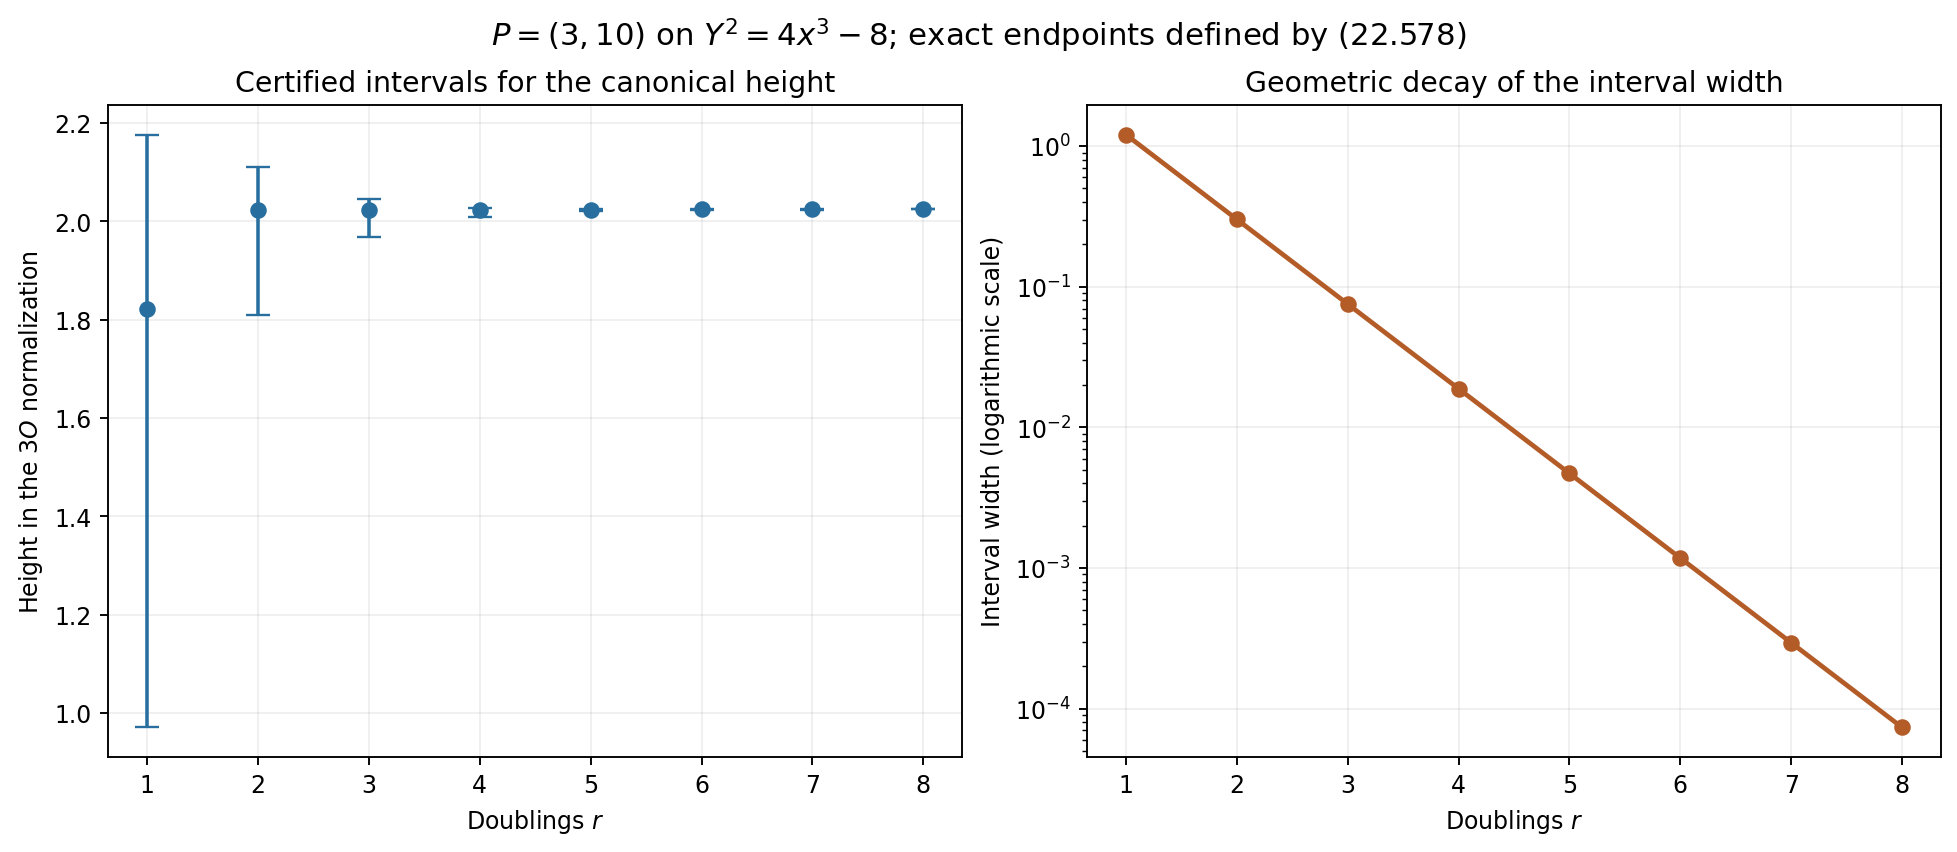
\includegraphics[keepaspectratio,alt={Intervals for the canonical height of a rational elliptic point}]{../verification/lesson22/elliptic-height-telescope.png}}
\par\smallskip
\begin{flushleft}\small
\emph{Figure 22.15. The intervals in (22.578) for successive doublings
of \((3,10)\) on \(Y^2=4x^3-8\). The endpoints are displayed
numerically; their defining integer recurrence and logarithmic
expressions are exact. The width decreases by a factor of four at every
step.}
\end{flushleft}
\end{minipage}\par\medskip


Canonical versus projective height estimates are used in S. David,
\href{https://smf.emath.fr/system/files/filepdf/MSMF_1995_2_62__1_0.pdf}{\emph{Minorations
de formes linéaires de logarithmes elliptiques}, Lemma 3.4}. The
estimates (22.571)--(22.572) use the explicit duplication certificates
displayed here and the plane-height normalization specified in (22.557).

\subsection{A uniform arithmetic estimate for the first elliptic
jet}\label{a-uniform-arithmetic-estimate-for-the-first-elliptic-jet}

Let \(E:y^2=x^3+Ax+B\) be nonsingular over a number field. Use plane
coordinates \([X:Y:Z]\), with identity \([0:1:0]\). Write \(Q=[u:v:w]\)
for a second point, so \(v^2w=u^3+Auw^2+Bw^3\). All logarithmic heights
use the absolute normalization of Lemma 22.47.

\subsubsection{Lemma 22.198. An explicit translation tuple at the
identity}\label{lemma-22.198.-an-explicit-translation-tuple-at-the-identity}

Define the following polynomials of bidegree \((2,2)\): \[
\begin{split}
 T_X={}&-Au^2Z^2+Aw^2X^2-3BuwZ^2+3Bw^2XZ\\
      &+2uvYZ+uwY^2-v^2XZ-2vwXY,\\
 T_Y={}&AuvZ^2-2AuwYZ+2AvwXZ-Aw^2XY\\
      &+3BvwZ^2-3Bw^2YZ-3u^2XY+3uvX^2-v^2YZ+vwY^2,\\
 T_Z={}&AuwZ^2-Aw^2XZ+3u^2XZ-3uwX^2-v^2Z^2+w^2Y^2.
\end{split}
\tag{22.579}
\] Where this tuple is nonzero it represents addition of the two points.
For every finite \(Q\), it is nonzero at the first identity, and \[
 T((0,1,0),Q)=wQ.
 \tag{22.580}
\] At an archimedean place the sum of the absolute coefficients of each
coordinate polynomial is at most \(20\max(1,|A|,|B|)\). At a finite
place its maximum coefficient modulus is at most \(\max(1,|A|,|B|)\).

\textbf{Proof.} On the affine open \(Z=w=1\), put \(d=x-u\) and
\(N_x=(y-v)^2-(x+u)d^2\). Reduction by the two curve equations gives the
three polynomial identities \[
 T_Z=d^3,\qquad T_X=dN_x,\qquad
 T_Y=-yd^3+(y-v)(xd^2-N_x).
 \tag{22.581}
\] For example, replace \(x^3\) by \(y^2-Ax-B\) and \(u^3\) by
\(v^2-Au-B\), and expand. The resulting expressions are exactly (22.579)
with \(Z=w=1\). When \(d\ne0\), the ratios are the chord formulas
\(x(P+Q)=N_x/d^2\) and \(y(P+Q)=-y+(y-v)(x-N_x/d^2)/d\). Homogenization
and equality of projective cross products extend this identity wherever
the tuple is nonzero. Substitution of \((X,Y,Z)=(0,1,0)\) gives
(22.580); a finite point has \(w\ne0\).

The three coefficient sums are bounded respectively by \(2|A|+6|B|+6\),
\(6|A|+6|B|+8\), and \(2|A|+8\). Each is at most the asserted
archimedean bound. All coefficients are integers times \(1,A,B\);
integers have finite-place modulus at most one. This proves the other
bound. At \(Q=O\), translation is instead represented by the identity
tuple \((X,Y,Z)\). Thus the displayed law supplies a frame near the
first identity for every translation. It is not asserted to be nonzero
at every pair of points. \(\square\)

\subsubsection{Proposition 22.199. A formal coefficient bound with
specified
constants}\label{proposition-22.199.-a-formal-coefficient-bound-with-specified-constants}

For \(1\le i\le g\), let \(E_i:y^2=x^3+A_ix+B_i\) and \(q_i\in E_i(L)\),
where \(L\) is a number field of degree \(e\). Put \[
 H_i=h(1:A_i:B_i),\qquad
 \mu_E=\sum_v w_v\log\max_i(1,|A_i|_v^{1/4},|B_i|_v^{1/6}),
 \qquad \mu_E\le\frac14\sum_iH_i.
 \tag{22.582}
\] Here \(w_v=[L_v:\mathbf Q_v]/e\). Normalize a representative \(Q_i\)
of each finite \(q_i\) to have one coordinate equal to one. Let
\(V_i(t)=(-t,1,-s_i(t))\), as in Lemma 22.163, and set
\(G_i(t)=T_i(V_i(t),Q_i)\). If \(q_i=O\), set \(G_i=V_i\).

Let \(P\) have multidegree \((d,D_1,\ldots,D_g)\), with nonnegative
integer degrees and \(N_P\ge1\) nonzero coefficients. For
\(a,\beta_i\in L\), put \[
 \mathscr H(t)=P\left(1,a+\sum_i\beta_i\ell_i(t_i),
                                  G_1(t_1),\ldots,G_g(t_g)\right),
 \qquad H_{a,\beta}=h(1:a:\beta_1:\cdots:\beta_g).
 \tag{22.583}
\] For \(|\nu|=N\), its coefficient \(c_\nu=[t^\nu]\mathscr H\)
satisfies \[
\begin{split}
 h(c_\nu)\le\mathcal B_N:={}&h_c(P)+\log N_P
       +d\{H_{a,\beta}+\log(g+1)\}\\
 &+\sum_iD_i\{2h(q_i)+H_i+\log20\}\\
 &+N(\log8+\mu_E)+\log\Delta_N(d).
\end{split}
\tag{22.584}
\] The denominator \(\Delta_N(d)\) is defined in Lemma 22.137. If
\(c_\nu\ne0\), then \(\log|c_\nu|\ge-e\mathcal B_N\) at any specified
complex embedding.

\textbf{Proof.} Put \(M_{i,v}=\max(1,|A_i|_v,|B_i|_v)\),
\(q_{i,v}=\max_j|Q_{i,j}|_v\), and let \(M_v\) be the maximum inside
(22.582). At a finite place, Lemmas 22.163 and 22.198 give \[
 |[t^m]G_{i,j}|_v\le M_{i,v}q_{i,v}^2M_v^m.
 \tag{22.585}
\] For \(q_i=O\), take \(q_{i,v}=1\); the same bound follows directly
from \(G_i=V_i\). At an infinite place, the series norm at radius
\((8M_v)^{-1}\) is at most \(20M_{i,v}q_{i,v}^2\), by the coefficient
sum in Lemma 22.198. The coefficient argument in Proposition 22.164 now
applies: an additive monomial uses at most \(d\) logarithm factors,
whose denominators divide \(\Delta_N(d)\), and its \(a,\beta\) degree is
at most \(d\). At infinity its series norm is bounded by
\(((g+1)\max(1,|a|_v,|\beta|_v))^d\). The \(N_P\) monomials contribute
the factor \(N_P\) at infinity. Taking weighted logarithms yields
exactly (22.584).

The inequality for \(\mu_E\) follows place by place from
\(M_v\le\prod_iM_{i,v}^{1/4}\). All constants are nonnegative and
unchanged by a field extension. The product-formula lower bound of Lemma
22.47 proves the assertion about a nonzero coefficient. This proof
includes \(N=0\), \(d=0\), and identity translations; in the first two
cases \(\Delta_N(d)=1\). \(\square\)

\subsubsection{Lemma 22.200. A lower bound for the entire lift at every
logarithm}\label{lemma-22.200.-a-lower-bound-for-the-entire-lift-at-every-logarithm}

Put \(a=-4A\), \(b=-4B\), and \[
 h_E=h(1:a:b),\qquad h_* =\max\{1,h_E,h(j(E))\}.
 \tag{22.586}
\] Let \(L_E=\omega_1(\mathbf Z+\tau\mathbf Z)\) be a reduced period
lattice for the differential \(dx/(2y)\). Use the entire tuple
\(\Phi_{L_E}\) of Theorem 22.179, in its coordinate order
\((\phi^3,\phi^3\wp,\phi^3\wp')\). The tuple \[
 \Psi_E(z)=\bigl(\Phi_{L_E,1}(z),
                       \tfrac12\Phi_{L_E,2}(z),
                       \Phi_{L_E,0}(z)\bigr)
 \tag{22.587}
\] represents \([x(z):y(z):1]\), and for every \(z\in\mathbf C\), \[
 \|\Psi_E(z)\|_\infty\ge \exp(-21eh_*).
 \tag{22.588}
\]

\textbf{Proof.} Write \(y_\tau=\operatorname{Im}\tau\). Proposition
22.186 gives \(y_\tau\le eh_*\). The discriminant estimate of
Proposition 22.185 and lattice scaling give \[
 |\omega_1|^{12}|a^3-27b^2|
 \ge0.89(2\pi)^{12}e^{-2\pi y_\tau},\qquad
 |a^3-27b^2|\le28e^{3eh_E}.
 \tag{22.589}
\] The constant \(0.89(2\pi)^{12}/28\) exceeds one, since \(2\pi>6\).
Therefore \(\log|\omega_1|\ge-(\pi/6+1/4)eh_*>-eh_*\). This argument
includes \(a=0\) and \(b=0\); the discriminant itself is nonzero.

In (22.528), \(J_\tau(w)=(\operatorname{Im}w-y_\tau/2)^2/y_\tau\ge0\).
The coordinate permutation and the factor \(1/2\) in (22.587) thus give
\[
 \|\Psi_E(z)\|_\infty
 \ge\frac{0.073^3}{2}
       \exp\{-(3+3\pi)eh_*\}.
 \tag{22.590}
\] Finally \(\log(2/0.073^3)<60/7\): the rational sum
\(\sum_{r=0}^{30}(60/7)^r/r!\) exceeds \(2/0.073^3\). Together with
\(\pi<22/7\), this implies \(3+3\pi+\log(2/0.073^3)<21\). Since
\(eh_*\ge1\), (22.590) proves (22.588). The argument is uniform in
\(z\), including lattice points and every choice of logarithm branch.
\(\square\)

\subsubsection{Theorem 22.201. A completely specified first-jet lower
bound}\label{theorem-22.201.-a-completely-specified-first-jet-lower-bound}

For the curves and polynomial of Proposition 22.199, write \(h_{*,i}\)
for (22.586). Choose logarithms \(v_i\) of \(q_i\) and use the lifts
\(\Psi_i\) from (22.587). Define \[
 F_q(z)=P\left(1,a+\sum_i\beta_i z_i,
                  \Psi_1(v_1+z_1),\ldots,\Psi_g(v_g+z_g)\right).
 \tag{22.591}
\] If its first nonzero total degree is \(N\), every nonzero
degree-\(N\) coefficient \(f_\nu\) satisfies \[
 \log|f_\nu|\ge
 -e\left(\mathcal B_N+21\sum_iD_i h_{*,i}\right).
 \tag{22.592}
\]

In particular, let \(p_i\in E_i(L)\) have logarithms \(u_i\), let
\(a=su_0\), \(q_i=[s]p_i\), \(v_i=su_i\), and let \(s\in\mathbf Z\).
Write \(H=h(1:u_0:\beta_1:\cdots:\beta_g)\) and choose real numbers
\(\mathcal V_i\ge\max\{h_{*,i},\widehat h_3(p_i)\}\), where
\(\widehat h_3\) has the normalization of (22.570). Then \[
\begin{split}
 \log|f_\nu|\ge-e\bigg[&h_c(P)+\log N_P
 +d\{H+\log((g+1)\max(1,|s|))\}\\
 &+\sum_iD_i(2s^2+48)\mathcal V_i\\
 &+N\left\{\log8+\frac14\sum_i(\mathcal V_i+\log4)
                  +2(\log2)H_{\min(d,N)}\right\}\bigg].
\end{split}
\tag{22.593}
\] Here \(H_m=\sum_{r=1}^m1/r\) and \(H_0=0\).

\textbf{Proof.} Normalize \(Q_i\) at a coordinate where \(\Psi_i(v_i)\)
has largest modulus. Thus all coordinates of \(Q_i\) have modulus at
most one at the chosen embedding, and \(\Psi_i(v_i)=\kappa_iQ_i\), with
\(|\kappa_i|=\|\Psi_i(v_i)\|_\infty\). For finite \(q_i\), Lemma 22.198
gives \(G_i(0)=b_iQ_i\), where \(b_i=Q_{i,Z}\ne0\) and \(|b_i|\le1\). At
\(q_i=O\), take \(Q_i=(0,1,0)\) and \(b_i=1\).

The first homogeneous part is unchanged by
\(z_i=\ell_i(t_i)=t_i+O(t_i^2)\), as proved in Proposition 22.138. The
two local lifts differ by holomorphic units, so the same first-degree
comparison as (22.462) gives \[
 f_\nu=c_\nu\prod_i(\kappa_i/b_i)^{D_i},\qquad c_\nu\ne0.
 \tag{22.594}
\] Use Proposition 22.199, \(|b_i|\le1\), and (22.588) to prove
(22.592). No estimate for the inverse translation scalar is needed.

For the sampled assertion, multiplication of one homogeneous coordinate
by \(s\) gives \(H_{su_0,\beta}\le H+\log\max(1,|s|)\), also for
\(s=0\). Changing from \([1:x:2y]\) to \([x:y:1]\) changes height by at
most \(\log2\). Corollary 22.196 therefore gives
\(h(q_i)\le(s^2+10)\mathcal V_i+\log2\). Also
\(H_i\le h_{E_i}+\log4\le\mathcal V_i+\log4\). Consequently \[
 2h(q_i)+H_i+\log20+21h_{*,i}
 \le(2s^2+42)\mathcal V_i+\log320
 <(2s^2+48)\mathcal V_i.
 \tag{22.595}
\] Here \(\log320<6\), as follows already by summing
\(\sum_{r=0}^{12}6^r/r!>320\). Finally use (22.582) and
\(\log\Delta_N(d)\le2(\log2)N H_{\min(d,N)}\) from Lemma 22.137. This
proves (22.593), including zero coordinates, torsion samples, negative
\(s\), \(d=0\), and \(N=0\). \(\square\)

\subsubsection{Exercise 22.202. Translation by a point of order
two}\label{exercise-22.202.-translation-by-a-point-of-order-two}

On \(E:y^2=x^3-x\), let \(q=(0,0)\). Find the tuple (22.579) for
translation by \(q\), prove that its square represents the identity
wherever defined, and compute its first jet at \(O\).

\textbf{Solution.} Substitution gives \[
 T_q(X,Y,Z)=(-X^2,XY,Y^2+XZ),\qquad
 T_q(T_q(X,Y,Z))=-X^3(X,Y,Z).
 \tag{22.596}
\] The second identity is a direct polynomial identity in three
independent variables. Thus the translation is an involution on a dense
open set, hence on the curve; \(q\ne O\) has order two. The tuple is
nonzero at \(O\), where it equals \((0,0,1)\).

Here \(s=t^3-ts^2=t^3-t^7+O(t^{11})\), so evaluation at
\(V(t)=(-t,1,-s(t))\) gives \[
 (x_q(t),y_q(t))=
 \left(\frac{-t^2}{1+ts(t)},\frac{-t}{1+ts(t)}\right),
 \qquad (x_q'(0),y_q'(0))=(0,-1).
 \tag{22.597}
\] This agrees with the invariant vector field \((2y,3x^2-1)\) at
\((0,0)\), since \(\ell'(0)=1\). In particular the \(y\)-coordinate has
first coefficient \(-1\). The local scalar is one even though \(q\) is a
point with zero \(y\)-coordinate. For \(P=Y\), (22.584) gives the
explicit upper bound \(\log160\) for the height of this coefficient; its
actual height is zero. \(\square\)

\begin{minipage}[t]{\linewidth}
\centering
\pandocbounded{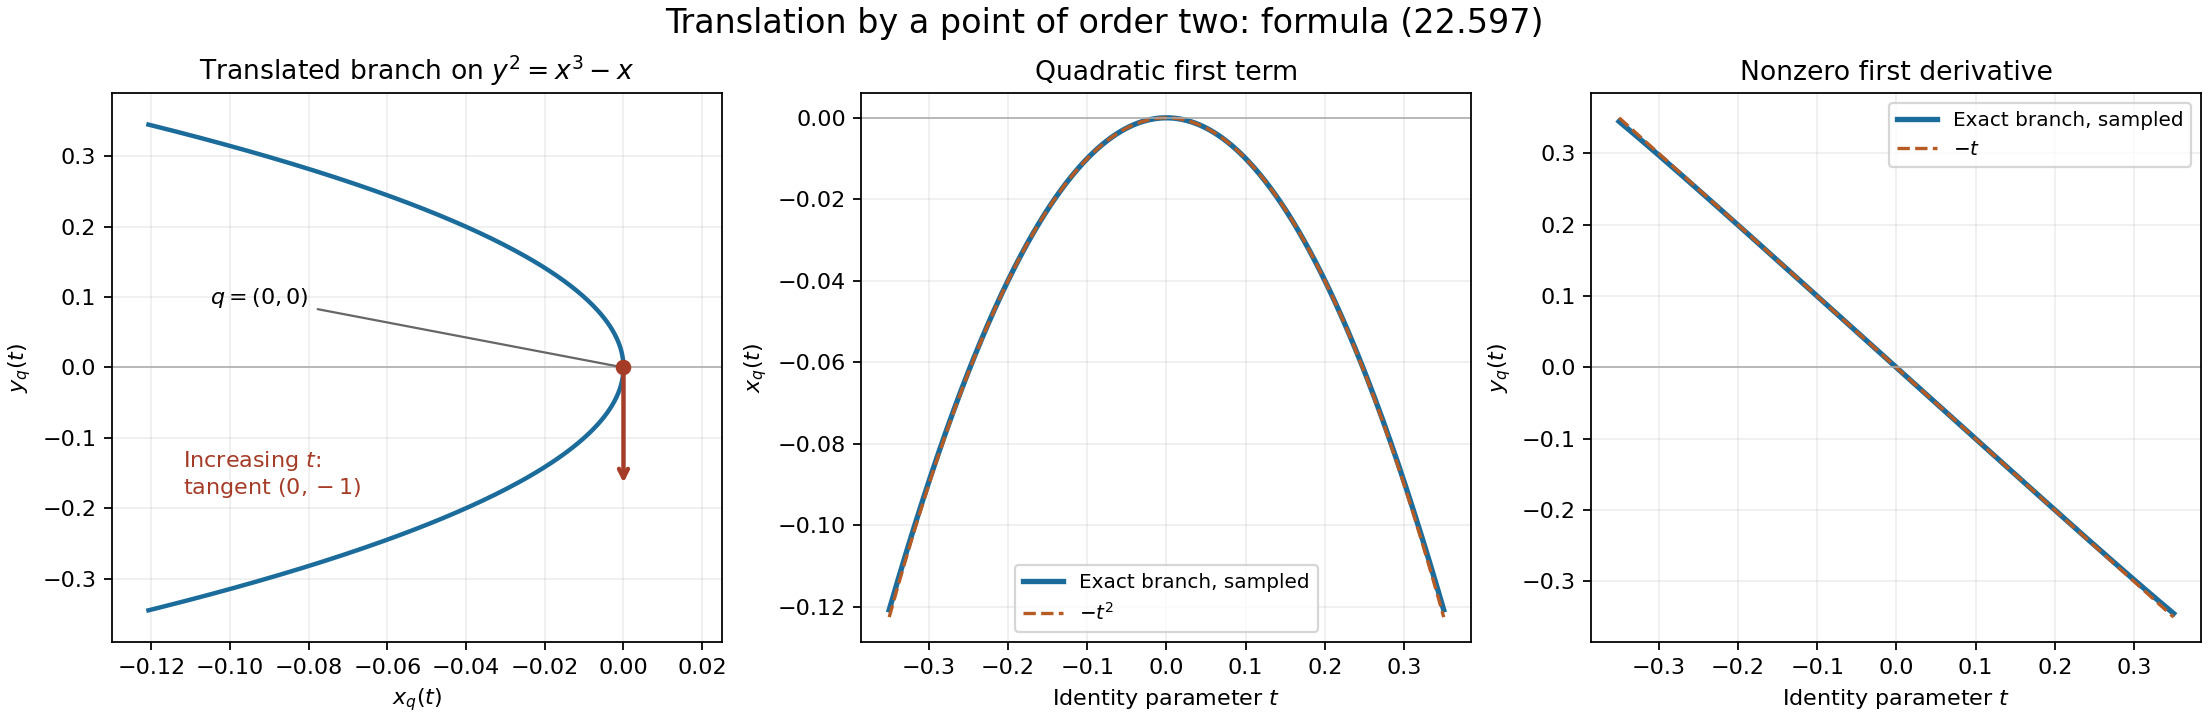
\includegraphics[keepaspectratio,alt={The local elliptic translation at a point of order two}]{../verification/lesson22/elliptic-two-torsion-translation.png}}
\par\smallskip
\begin{flushleft}\small
\emph{Figure 22.16. The map in (22.597) sends a neighborhood of the
identity, parametrized by \(t\), to the branch through \((0,0)\). The
left panel shows its image and the tangent direction for increasing
\(t\). The two right panels show the coordinate functions and their
first terms \(-t^2\) and \(-t\). The algebraic formula and the
derivative are exact; plotted points are numerical evaluations of the
formal branch.}
\end{flushleft}
\end{minipage}\par\medskip


The first-jet method is discussed in É. Gaudron,
\href{https://lmbp.uca.fr/~gaudron/art4.pdf}{\emph{Mesures
d'indépendance linéaire de logarithmes dans un groupe algébrique
commutatif}}, Sections 6.11--6.13. The entire-coordinate bounds used
here are proved in Theorems 22.179 and 22.182, with comparison to S.
David,
\href{https://smf.emath.fr/system/files/filepdf/MSMF_1995_2_62__1_0.pdf}{\emph{Minorations
de formes linéaires de logarithmes elliptiques}}, Proposition 3.1. All
constants in (22.593) are specified by the displayed curve, polynomial
and height data.

\subsection{Numerical weights and a stronger multiplicity
estimate}\label{numerical-weights-and-a-stronger-multiplicity-estimate}

Let \(g\ge1\), \(n=g+1\), and let \(E_i\) and \(p_i\in E_i(K)\) be
elliptic curves and points over a number field \(K\) of degree \(D\), in
the models of (22.557) and (22.586). Choose nonzero complex logarithms
\(u_i\) of \(p_i\). Put \(h=\max_i h_{*,i}\). Choose real height budgets
\(v_i\) and parameters \(B,E\) satisfying \[
\begin{gathered}
 b=\log B\ge \mathrm e h,\qquad
 Db\ge v_1\ge\cdots\ge v_g\ge h,\qquad
 v_i\ge\widehat h_3(p_i),\qquad \ell=\log E\ge1,\\
 E\le\frac{\mathrm e\sqrt{Dv_i}\,|\omega_{1,i}|
                       \sqrt{\operatorname{Im}\tau_i}}
                    {\sqrt{3\pi}\,|u_i|}\quad(1\le i\le g).
\end{gathered}
\tag{22.598}
\] The requirement \(u_i\ne0\) makes each denominator meaningful. Terms
with zero logarithm can be omitted before choosing these parameters.
Throughout this section \(\mathrm e=\exp(1)\).

\subsubsection{Lemma 22.203. A height bound for the analytic
parameter}\label{lemma-22.203.-a-height-bound-for-the-analytic-parameter}

Under (22.598), \[
 \ell\le5Dv_g,\qquad
 L=\log b+h+\log D+\ell\le
 R=b+\log D+\ell,\qquad L\ge\ell.
 \tag{22.599}
\]

\textbf{Proof.} Fix one index, write \(H=Dv_i\ge1\),
\(y=\operatorname{Im}\tau_i\), \(\omega=\omega_{1,i}\), and
\(r=|u_i/\omega|>0\). Proposition 22.186 gives \(y\le H\). If
\(r\ge1/10\), (22.598) gives \(\ell\le1+\log H+\log(10/3)<3H\), since
\(\pi>3\), \(\log H\le H-1\), and \(\log(10/3)<2\).

Suppose \(r<1/10\). A nonzero point of a reduced normalized lattice has
modulus at least one, by the shortest-vector construction in Proposition
22.186. Thus \(p_i\ne O\). Proposition 22.190 gives
\(|u_i|^2\ge0.9/|x(p_i)|\). The canonical-height bound (22.567) implies
\[
 h_x(p_i)\le\tfrac23\widehat h_3(p_i)
                +\tfrac53h_{E_i}+\tfrac13\log27648\le6v_i.
 \tag{22.600}
\] Here \(\log27648<11\), as is certified by the positive sum
\(\sum_{j=0}^{25}11^j/j!>27648\).

We also have \(\log(|\omega|\sqrt y/\sqrt{3\pi})\le H/3\). For a nonzero
invariant \(a_i\), (22.544) gives
\(\log|\omega|\le1.85-\tfrac14\log12-\pi y/6+H/3\). The maximum of
\(\tfrac12\log y-\pi y/6\) is \(\tfrac12\log(3/\pi)-1/2\), by
differentiation. The remaining constant is
\(1.35-\tfrac14\log12-\log\pi<0\): use \(\pi>3\), \(\mathrm e<3\), and
\(9<12\). If \(a_i=0\), then \(j(E_i)=0\), hence \(y\le1\) by
Proposition 22.186. The bound \(|g_3(\tau_i)|<1005\) gives
\(\log|\omega|\le(\log1005+H)/6\). Since
\(1005<2\cdot729<\mathrm e(3\pi)^3\), the same assertion follows from
\(H\ge1\).

The height bound for a complex coordinate now yields \[
 \ell\le1+\tfrac12\log H+\tfrac D2h_x(p_i)
              +H/3+\tfrac12\log(10/9)<\tfrac92H<5H.
 \tag{22.601}
\] Indeed \(1+\tfrac12\log H\le H\) and \(\tfrac12\log(10/9)<1/6\),
because \(\exp(1/3)>1+1/3>10/9\). Apply the result to every index.
Finally \(b\ge\mathrm e\) gives \(\log b\le b/\mathrm e\), by maximizing
\(\log t/t\). Also \(h\le b/\mathrm e\). Thus
\(\log b+h\le2b/\mathrm e<b\), proving the last claims of (22.599).
\(\square\)

\subsubsection{Lemma 22.204. Explicit preliminary
degrees}\label{lemma-22.204.-explicit-preliminary-degrees}

Define positive constants, depending only on \(g\), by \[
\begin{gathered}
 \epsilon=\frac1{200g^2},\quad \lambda=2\epsilon,\quad
 A_g=g\log(4n)+5\log n+15,\\
 J_g=\frac{12(13+4\mathrm e^2)}{25+4\mathrm e^2}
                  n\log(4n)+56\log n+54,\\
 c_4=4^g n^{g+1}(1+\lambda)8n A_gJ_g,\qquad c_6=n2^g,\\
 c_7=\frac{4\log(4n)}{13+4\mathrm e^2}
          +\frac{60+20\log n}{(13+4\mathrm e^2)g},\qquad
 c_5=\frac{c_6c_4^{2g+1}}{n!6^gc_7^g}.
\end{gathered}
\tag{22.602}
\] Set \[
\begin{gathered}
 S=\left\lfloor\frac{c_4DL}{\ell}\right\rfloor,\qquad
 U_0=c_5D^{2g+2}RL^{g+1}\left(\prod_i v_i\right)\ell^{-2g-1},\\
 \Theta=\frac{U_0}{DL},\qquad
 t_i=\frac{c_7U_0}{DS^2v_i}\quad(1\le i\le g),\qquad
 C=(1+\epsilon)2^g.
\end{gathered}
\tag{22.603}
\] These numbers satisfy \[
\begin{gathered}
 \frac{c_4DL}{2\ell}\le S\le\frac{c_4DL}{\ell},\qquad
 \Theta>800g^3n,\quad \Theta\ge c_4,\quad t_i>400g^3+1,\\
 M:=\min_i\frac{\Theta}{t_i}
       =\frac{S^2v_g}{c_7L}\ge\frac{c_4^2}{20c_7}>6n.
\end{gathered}
\tag{22.604}
\]

\textbf{Proof.} The elementary estimates \[
 c_4\ge6480\,4^gn^{g+2},\qquad c_4>10^5n^2,
 \qquad 0<c_7<5n
 \tag{22.605}
\] are useful. The first uses \(A_g>15\), \(J_g>54\). For the second,
\(\log2>3/5\) follows from \(\mathrm e<3\) and \(3^3<2^5\). Hence
\(A_g>19\), \(J_g>85\), and \(4^gn^g\ge8\), giving \(c_4>103360n^2\).
For the last use \(\log(4n)\le2n\), \(\log n\le n\), and \(n\ge2\): the
numerator defining \(c_7\), with \(1/g\le1\), is at most
\(28n+60\le58n\), while its denominator exceeds 13.

Since \(DL/\ell\ge1\), taking the floor loses at most half. Moreover
(22.599) gives \(v_i\ge\ell/(5D)\). Substitution into (22.603), using
\(R,L\ge\ell\), gives \[
 \Theta\ge c_5/5^g,\qquad
 t_i\ge\frac{c_7c_5}{5^{g-1}c_4^2}.
 \tag{22.606}
\] Using \(n!\le n^n\), \(c_7<5n\), and \(c_6\ge1\), the first bound is
greater than \(10^5n^{2g+1}\), and its ratio to \(c_4\) is at least
\(c_4^{2g}/(150^gn^{2g+1})>1\). Since \(n^{2g}\ge g^3\), this proves
both assertions about \(\Theta\). The second bound is at least \[
 \frac{c_4^{2g-1}}{150^gn^{2g}}
 >\frac{2000}{3}\left(\frac{10^{10}}{150}\right)^{g-1}
          n^{2g-2}\ge\frac{2000}{3}g^3>400g^3+1.
 \tag{22.607}
\] For \(g=1,2\), the penultimate comparison is direct; for \(g\ge3\),
use \(2g-2\ge3\) and \(n\ge g\). Finally the lower bound for \(S\),
followed by \(v_g\ge\ell/(5D)\) and \(L\ge\ell\), proves the bound for
\(M\). In fact (22.605) gives \(c_4^2/(20c_7)>10^8n^3>6n\). \(\square\)

\subsubsection{Proposition 22.205. An extremal additive
degree}\label{proposition-22.205.-an-extremal-additive-degree}

Let \(p\in G=\mathbf G_a\times\prod_iE_i\), and let
\(W=\{z_0=\sum_i\beta_i z_i\}\), with every \(\beta_i\ne0\). For each
connected subgroup \(H=\{0\}\times B\) whose Lie algebra is contained in
\(W\), put \(h_B=\dim B\), \(q_B=g-h_B\), and
\(Q_B=\#\{sp+H:0\le s<S\}\). Write \(P_q(z)=\prod_{j=1}^q(z+j)\), and
define \[
 t_0=\min_B
 \frac{P_{q_B}(\Theta)Q_B\mathcal H_B(t_1,\ldots,t_g)}
                 {C n!3^g\prod_i t_i}.
 \tag{22.608}
\] The minimum exists, is attained, and satisfies \[
 400g^3+1<t_0\le\frac{U_0}{c_6DR},\qquad
 P_{q_B}(\Theta)Q_B\mathcal H_B(t)\ge C\mathcal H_G(t)
 \tag{22.609}
\] for every such \(B\), with equality for a minimizing \(B_*\). Every
integer \(L_i=\lfloor t_i\rfloor\), including \(i=0\), is greater than
\(400g^3\).

\textbf{Proof.} The multidegree polynomials in Proposition 22.149 have
nonnegative integer coefficients and a positive coefficient. At fixed
positive weights, a bounded value bounds each of those integers. The
dimension has finitely many possibilities and \(1\le Q_B\le S\). Hence
the same finite-coefficient argument as in Lemma 22.151 gives a positive
attained minimum.

For the point subgroup, \(\mathcal H_{\{0\}}=1\) and \(Q_{\{0\}}\le S\).
Direct substitution of (22.602)--(22.603) shows that its value divided
by \(U_0/(c_6DR)\) is at most \[
 \frac1{1+\epsilon}\prod_{j=1}^g(1+j/\Theta)\le1.
 \tag{22.610}
\] Indeed \(\sum j/\Theta<\epsilon/8\), by (22.604), and
\(\prod(1+x_j)\le\exp(\sum x_j)\le1+\epsilon/4\). The last step follows
from \(e^x\le(1-x)^{-1}\le1+2x\) for \(0\le x\le1/2\). This proves the
upper bound.

At a minimizing subgroup of dimension \(h_B\), set \(q=g-h_B\ge1\). A
positive monomial of \(\mathcal H_B\) has coefficient at least
\(h_B!3^{h_B}\). Equality in (22.609) and \(P_q(\Theta)\ge\Theta^q\)
give \[
 t_0\ge\frac{h_B!}{Cn!}
                  \left(\frac{c_4^2}{60c_7}\right)^q.
 \tag{22.611}
\] Put \(A=c_4^2/(60c_7)\). There are \(q+1\) factors in \(n!/h_B!\),
each at most \(n\), and \(A>n\). Thus the right side is at least
\(A/(Cn^2)\). From (22.605) and \(C<2^{g+1}\), this exceeds
\(69984\,8^gn^{2g+1}>400g^3+1\). The remaining assertions follow from
the definition of the minimum and (22.604). \(\square\)

\subsubsection{Lemma 22.206. Counting powers of an
ideal}\label{lemma-22.206.-counting-powers-of-an-ideal}

Let \(R\) be a regular local ring of dimension \(r\), containing a
characteristic-zero field. Let \(I\) be primary for its maximal ideal.
Suppose \(\rho\) transverse derivations, normalized as in (22.61), send
every element of \(I\) into the maximal ideal after every word of length
at most \(T\). Assume that these derivations extend to a set of \(r\)
derivations dual modulo the maximal ideal to a regular parameter system.
If a parameter ideal \(J\subset I\) is generated by a regular sequence,
then \[
 \operatorname{length}(R/J)\ge(T+1)^\rho.
 \tag{22.612}
\] The assertion includes \(\rho=0\).

\textbf{Proof.} Put \(a=T+1\). For a word applied to a product of \(m\)
elements of \(I\), call the first \(\rho\) derivations the selected
ones. If it has \(b\) other derivations and fewer than \(a(m-b)\)
selected derivations, one of the \(m\) factors receives no other
derivation and at most \(T\) selected ones. Every term of the product
rule therefore vanishes in the residue field. This applies to every
element of \(I^m\).

Use the filtration and coefficient-lifting proof of Theorem 22.25, now
with all \(r\) parameters. In each ordinary degree it proves
independence, modulo \(I^m\) and the next maximal-ideal power, of the
monomials \(z^\alpha\) satisfying \[
 |\alpha_{1:\rho}|<a\bigl(m-|\alpha_{\rho+1:r}|\bigr).
 \tag{22.613}
\] For each selected multiindex, use the word with those exact
derivation counts. The normalized linear action kills every other
monomial of the same total degree, just as in (22.64). Consequently
\(\operatorname{length}(R/I^m)\) is at least the number \(N_m\) of these
monomials.

If \(0<\rho<r\), this count is \[
 N_m=\sum_{b=0}^{m-1}
       \binom{b+r-\rho-1}{r-\rho-1}
       \binom{a(m-b)+\rho-1}{\rho},\qquad
 \lim_{m\to\infty}\frac{r!N_m}{m^r}=a^\rho.
 \tag{22.614}
\] To obtain the limit, use the leading terms of the two binomial
polynomials and the Riemann sum on \([0,1]\). Repeated integration by
parts gives \(\int_0^1t^{r-\rho-1}(1-t)^\rho dt
=(r-\rho-1)!\rho!/r!\). For \(\rho=r\), the count is
\(\binom{am+r-1}{r}\); for \(\rho=0\), it is \(\binom{m+r-1}{r}\). These
give the same limit.

We spell out the corresponding regular-sequence count. If
\(J=(f_1,\ldots,f_r)\), then \(J^d/J^{d+1}\) is free over \(R/J\) on the
degree-\(d\) monomials in the \(f_i\). Here is an induction proof. For
\(I'=(f_1,\ldots,f_{r-1})\), the induction hypothesis gives the same
description of its graded pieces. Since \(f_r\) is regular on \(R/I'\),
it is regular on each such piece and hence on \(R/I'^m\). It follows
that \((I'^m:f_r)=I'^m\). Expanding \(J^{m+1}=\sum_jf_r^jI'^{m+1-j}\)
then gives \((J^{m+1}:f_r)=J^m\). To prove independence of the
degree-\(d\) monomials, reduce a relation modulo \(f_r\). The induction
hypothesis for the regular sequence in \(R/(f_r)\) puts the coefficients
of the terms without \(f_r\) in \(J\). Remove these terms, divide the
remainder by \(f_r\), and use the colon identity and induction on \(d\).
All coefficients lie in \(J\). Permutation of a regular sequence in a
local ring is the proved Proposition 1.2 of
\href{../AG-CA/AG-CA-12.html}{\emph{Regular sequences, depth and
Cohen--Macaulay modules}}. The base case is cancellation of a
nonzerodivisor.

Adding the graded lengths gives \[
 \operatorname{length}(R/J^m)
   =\binom{m+r-1}{r}\operatorname{length}(R/J).
 \tag{22.615}
\] Since \(J^m\subset I^m\), this is at least \(N_m\). Divide by
\(m^r/r!\) and use (22.614) to prove (22.612). \(\square\)

\subsubsection{Theorem 22.207. A multiplicity estimate from
powers}\label{theorem-22.207.-a-multiplicity-estimate-from-powers}

Use the notation and hypotheses of Theorem 22.159, so that a nonzero
section of multidegree \(L\) vanishes to order at least \(nT+1\) along
\(W\) on \(\Sigma(n)\). There is a connected proper subgroup \(H\), of
codimension \(r\), such that, with
\(\rho=\dim W-\dim(W\cap\operatorname{Lie}H)\), \[
 (T+1)^\rho\,\#\{s+H:s\in\Sigma\}\,
                 \mathcal H_H(L)
       \le2^{r-1}\mathcal H_G(L).
 \tag{22.616}
\]

\textbf{Proof.} Repeat the ideal chain and the finite-coset construction
of Theorem 22.159 through (22.439), keeping the ideal \(\mathcal J\) and
its coset components rather than the numerical length bound. Choose
\(v_0\in V\), and replace \(\mathcal J\) by \(t_{-v_0}^*\mathcal J\).
This ideal contains the original section \(P\): the summand with
translation \(v_0\) contains \(t_{v_0}^*P\). Its zero set is the
translate of the same finite union of cosets, with the same degrees and
derivative conditions.

In the embedding given by \(\mathcal L_L\), \(P\) has degree one, and
the translated ideal has quadratic generators by Lemma 22.157. Start the
complete intersection with \(P\), then choose \(r-1\) linear
combinations of those quadrics. At each stage before codimension \(r\),
no component of the current intersection is contained in the ideal's
zero set, whose pure codimension is \(r\). Avoiding the finitely many
corresponding proper linear conditions chooses the next equation. The
regular-sequence argument of Lemma 22.30 applies.

At the generic point of each retained coset, the localized ideal is
primary in a regular local ring of dimension \(r\). The \(W\)-directions
have transverse rank \(\rho\). Normalize them as in Corollary 22.26, and
extend them to \(r\) transverse derivations using invariant vector
fields of the smooth group. The coefficient changes preserve the
derivative-vanishing condition by the product rule. Lemma 22.206 gives
intersection length at least \((T+1)^\rho\).

Lemma 22.30 bounds the total weighted degree by
\(1\cdot2^{r-1}\mathcal H_G(L)\). There are at least \(\#(\Sigma+H)/H\)
retained cosets, all of degree \(\mathcal H_H(L)\). This proves
(22.616). \(\square\)

\subsubsection{Corollary 22.208. The explicit weights force a nonzero
jet}\label{corollary-22.208.-the-explicit-weights-force-a-nonzero-jet}

Choose \(t_0\) by Proposition 22.205, let \(L_i=\lfloor t_i\rfloor\),
and put \(T=\lfloor\Theta\rfloor\). Every section of this multidegree
that is not identically zero on \(G\) has a nonzero \(W\)-jet of order
at most \(nT\) at some \(sp\), where \(0\le s\le n(S-1)\).

\textbf{Proof.} Suppose all these jets vanish. Apply (22.616) with
\(\Sigma=\{sp:0\le s<S\}\). First suppose
\(\operatorname{Lie}H\subset W\). Write \(H=0\times B\), \(q=g-\dim B\),
and \(\eta=(400g^3+1)^{-1}\). Since \(L_i>(1-\eta)t_i\), \(T+1>\Theta\),
and \(P_q(\Theta)\le(1+\epsilon/4)\Theta^q\), (22.609) gives \[
 \frac{(T+1)^qQ_B\mathcal H_B(L)}{2^g\mathcal H_G(L)}
 \ge\frac{(1+\epsilon)(1-\eta)^{\dim B}}
                 {1+\epsilon/4}
 \ge\frac{(1+\epsilon)(1-\epsilon/2)}{1+\epsilon/4}>1.
 \tag{22.617}
\] The second inequality uses Bernoulli's inequality and
\(g\eta<\epsilon/2\); the last uses \(\epsilon<1/2\). This contradicts
(22.616), since \(r-1\le g\).

Otherwise \(\rho=r\), since \(W\) is a hyperplane. Every connected
subgroup is either \(0\times B\) or \(\mathbf G_a\times B\), by Lemma
22.71. The multidegree calculation of Proposition 22.149 applies to an
arbitrary abelian subvariety \(B\); only its final assertion about an
omitted coordinate required \(\operatorname{Lie}H\subset W\).

If \(H=0\times B\) has dimension \(h_B=n-r\), choose one positive
monomial of its multidegree polynomial. Cancel its coordinates from
(22.616), use \(Q_B\ge1\), and use \(L_i\le t_i\). The result is \[
 1\le\frac{2^{r-1}n!3^{r-1}}{h_B!}
       \frac{t_0}{\Theta}
       \prod_{j\notin I}\frac{t_j}{\Theta}
 \le\frac1{2^g}\frac LR
               \left(\frac{6n}{M}\right)^{r-1}<1.
 \tag{22.618}
\] Here \(|I|=h_B\), \(t_0/\Theta\le L/(c_6R)\), and there are \(r-1\)
missing elliptic coordinates. The factorial ratio is at most \(n^r\). If
\(H=\mathbf G_a\times B\), the additive degree cancels instead; the same
calculation gives \[
 1\le\frac12\left(\frac{6n}{M}\right)^r<1.
 \tag{22.619}
\] Indeed its dimension is \(n-r\) and its multidegree has a positive
monomial with coefficient \((n-r)!3^{g-r}\) times \(L_0\). Both
contradictions use \(M>6n\). No possible subgroup remains, proving the
assertion. \(\square\)

\subsubsection{Proposition 22.209. Explicit small-rank sampling
ranges}\label{proposition-22.209.-explicit-small-rank-sampling-ranges}

For a minimizing \(B_*\), put \(h_B=\dim B_*\), \(q=g-h_B\), and
\(Q=Q_{B_*}\). The following two systems of jets have rank at most
\((1+\epsilon)\dim H^0(X,\mathcal L_L)/J_g\):

\begin{itemize}
\tightlist
\item
  If \(Q=S\), use all jets of total order at most \(nT\) at \(sp\),
  \(0\le s<S_0\), where
  \(S_0=\lfloor S/((1+\lambda)4^gn^{g+1}J_g)\rfloor\).
\item
  Choose a basis of \(W\) beginning with \(\operatorname{Lie}B_*\), and
  designate one normal direction. Use points \(sp\), \(0\le s<2nS\), and
  all jets of total order at most \(nT\) with designated exponent less
  than \(T_0=\lfloor\Theta/(2g(1+\lambda)4^gn^{g+1}J_g)\rfloor\).
\end{itemize}

Both \(S_0\) and \(T_0\) are positive.

\textbf{Proof.} The ratio \(\mathcal H_G(t)/\mathcal H_G(L)\) is at most
\((1-\eta)^{-n}\le1+\lambda\). Indeed
\((1-\eta)^n\ge1-n\eta\ge(1+\lambda)^{-1}\); the last inequality is
\(n(100g^2+1)\le400g^3+1\). The rank formula (22.404), the extremal
equality, and \(\dim H^0(X,\mathcal L_L)\ge\mathcal H_G(L)/n!\) bound
the rank divided by this dimension by \[
 C(1+\lambda)\frac{n!}{h_B!}\frac cQ
                 \frac{|\mathcal A|}{P_q(\Theta)}.
 \tag{22.620}
\] For total order \(nT\), the last fraction is at most \(n^q/q!\).
Since \(n!/(h_B!q!)=n\binom gq\le n2^g\), the first assertion follows
from \(c\le S_0\).

In the second case, at most \(2nQ\) cosets occur, as in Corollary
22.152. The last fraction in (22.620) is at most
\((T_0/\Theta)n^{q-1}/(q-1)!\). Using \(n!/(h_B!(q-1)!)=nq\binom gq\)
gives the asserted bound from the definition of \(T_0\).

Finally the denominator defining \(S_0\) equals \(c_4/(8nA_g)\), so
(22.604) gives a quotient at least \(4nA_g>1\). The denominator defining
\(T_0\) equals \(gc_4/(4nA_g)\); since \(\Theta\ge c_4\), its quotient
is at least \(4nA_g/g>1\). \(\square\)

\subsubsection{Exercise 22.210. A power count in two transverse
directions}\label{exercise-22.210.-a-power-count-in-two-transverse-directions}

In \(R=\mathbf Q[x,y]_{(x,y)}\), put \(I=(x,y)^4\). Compute
\(\operatorname{length}(R/I^m)\), and show that every regular-sequence
parameter ideal \(J\subset I\) has colength at least 16. Give a
parameter ideal attaining this value.

\textbf{Solution.} The monomials with total degree less than \(4m\) form
a basis of \(R/I^m\), hence \[
 \operatorname{length}(R/I^m)=\binom{4m+1}{2}=8m^2+2m,
 \qquad \lim_{m\to\infty}\frac{2\operatorname{length}(R/I^m)}{m^2}=16.
 \tag{22.621}
\] Equation (22.615) and \(J^m\subset I^m\) give the lower bound 16. The
regular sequence \((x^4,y^4)\) lies in \(I\); its quotient has the 16
basis monomials \(x^iy^j\), \(0\le i,j<4\). In contrast
\(\operatorname{length}(R/I)=10\). The leading count of the powers
therefore gives a stronger intersection bound than the first colength
alone. \(\square\)

\begin{minipage}[t]{\linewidth}
\centering
\pandocbounded{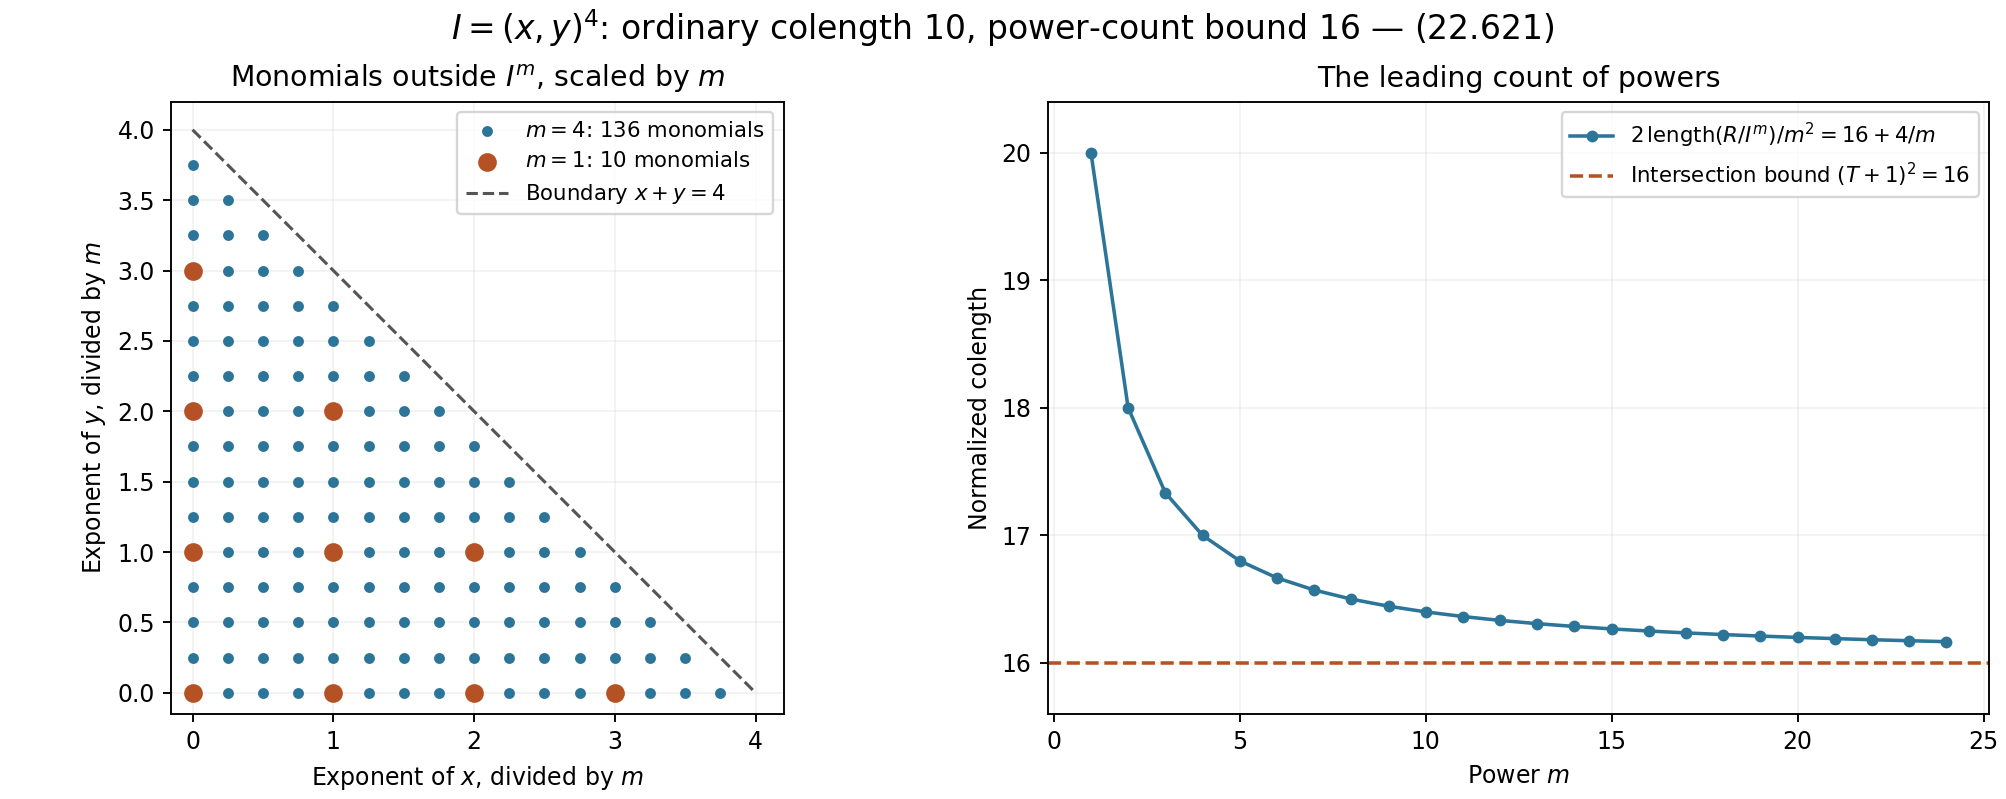
\includegraphics[keepaspectratio,alt={Lattice counts for powers of a transverse ideal}]{../verification/lesson22/elliptic-parameter-region.png}}
\par\smallskip
\begin{flushleft}\small
\emph{Figure 22.17. For \(I=(x,y)^4\), the scaled monomials outside
\(I^m\) fill the triangle \(x+y<4\). Its area is eight. Twice the
monomial count divided by \(m^2\) tends to 16, the intersection lower
bound in Exercise 22.210. The finite counts and the limiting value
follow from (22.621).}
\end{flushleft}
\end{minipage}\par\medskip


The parameter shape and extremal additive degree are those of S. David,
\href{https://smf.emath.fr/system/files/filepdf/MSMF_1995_2_62__1_0.pdf}{\emph{Minorations
de formes linéaires de logarithmes elliptiques}}, Section 5. The
estimate \(\ell\le5Dv_g\) and the complete rounding arguments above use
the height bounds proved here. The use of powers to retain multiplicity
is related to A. Galateau,
\href{https://www.numdam.org/item/10.5802/pmb.3.pdf}{\emph{Un théorème
de zéros dans les groupes algébriques commutatifs}}, Section 2.1. Lemmas
22.206--22.207 give the local count and intersection argument needed for
(22.616) explicitly.

\subsection{Numerical auxiliary
sections}\label{numerical-auxiliary-sections}

Use the parameters of Propositions 22.203--205. In particular,
\(n=g+1\), \(T=\lfloor\Theta\rfloor\), \(L_i=\lfloor t_i\rfloor\), and
\(L=\log b+h+\log D+\ell\), whereas \(L_i\) denotes an integer degree.
Write \[
 \kappa=1+\epsilon,\qquad
 \mathcal M=(L_0+1)3^g\prod_{i=1}^gL_i,
 \qquad Z_g=(1+\lambda)4^gn^{g+1}J_g.
 \tag{22.622}
\] Thus \(\mathcal M\) is the dimension of the space of sections on the
product of the additive projective line and the plane cubics. Its
monomial basis is the basis of Proposition 22.149. For the long
Weierstrass equation, division by the cubic after normalizing its
leading coefficient to one gives the same condition: the exponent of the
elliptic \(X_i\) is at most two.

\subsubsection{Proposition 22.211. Sampling through twice the target
order}\label{proposition-22.211.-sampling-through-twice-the-target-order}

Let \(B_*\) minimize (22.608), put \(j=\dim B_*\), \(q=g-j\), and write
\(Q=Q_{B_*}\). Set \[
 S_0=\lfloor S/Z_g\rfloor,\qquad
 T_0=\lfloor\Theta/(gZ_g)\rfloor.
 \tag{22.623}
\] Both integers are positive. The following are bounds for the complex
rank of the indicated systems of divided \(W\)-jets:

\begin{itemize}
\tightlist
\item
  If \(Q=S\), use all orders at most \(2nT\) at the points \(sp\),
  \(0\le s<S_0\). Their rank is at most
  \(\kappa\mathcal M/(2^j j!J_g)\).
\item
  In a basis beginning with \(\operatorname{Lie}B_*\), designate one of
  its normal directions. Use \(0\le s<2nS\), all total orders at most
  \(2nT\), and designated exponent less than \(T_0\). Their rank is at
  most \(\kappa(q/g)\mathcal M/(2^j j!J_g)\).
\end{itemize}

\textbf{Proof.} Put \(P_q(X)=\prod_{a=1}^q(X+a)\). The rank ratio in
(22.620) remains valid for either normal index set. Multiplication by an
analytic trivializing unit changes a divided jet only by an invertible
triangular combination of its lower jets. The two index sets are
downward closed, so the rank bound applies equally to the entire lifts
used below. For the first set, \[
 \frac{\binom{2nT+q}{q}}{P_q(\Theta)}
 \le\frac{(2n)^q}{q!},\qquad
 \frac{n!}{j!q!}=n\binom gj\le\frac{n^{j+1}}{j!}.
 \tag{22.624}
\] The first inequality follows factor by factor from
\(2nT+a\le2n(\Theta+a)\). The second follows by writing
\(\binom gj=g(g-1)\cdots(g-j+1)/j!\) and bounding each numerator by
\(n\); the empty product is one. Since there are at most \(S_0\) cosets,
substitution in (22.620) gives the first bound: the powers of two leave
\(2^{g+q}/4^g=2^{-j}\), and the powers of \(n\) cancel.

For the second set, summing over the designated exponent gives \[
 \frac{|\mathcal A|}{P_q(\Theta)}
 \le\frac{T_0}{\Theta}\frac{(2n)^{q-1}}{(q-1)!},
 \qquad
 \frac{n!}{j!(q-1)!}\le\frac{q n^{j+1}}{j!}.
 \tag{22.625}
\] Indeed each summand is at most \(\binom{2nT+q-1}{q-1}\); cancel its
\(q-1\) factors against the first factors of \(P_q\), and bound the
remaining factor below by \(\Theta\). This also proves the formula when
\(q=1\). There are at most \(2nQ\) cosets among these points: if the
order of the coset of \(p\) is below \(S\), it is \(Q\); otherwise
\(Q=S\) and there are at most \(2nS\) points. Substitution proves the
second bound.

Finally \(Z_g=c_4/(8nA_g)\). The lower bound for \(S\) in (22.604) and
\(DL/\ell\ge1\) give \(S/Z_g\ge4nA_g>1\). Since \(\Theta\ge c_4\),
\(\Theta/(gZ_g)\ge8nA_g/g>1\). Taking floors therefore gives positive
integers. \(\square\)

\subsubsection{Lemma 22.212. The coefficient field and its height
budget}\label{lemma-22.212.-the-coefficient-field-and-its-height-budget}

Assume the normalized coefficients satisfy \(|u_0|,|\beta_i|\le1\) and
\(H=h(1:u_0:\beta_1:\cdots:\beta_g)\le nb\). Let \(K_0\) be the subfield
generated over \(\mathbf Q\) by these coefficients, all curve
coefficients \(g_{2,i},g_{3,i}\), and the affine coordinates of the
finite points \(p_i\). Points equal to the identity require no
coordinates. Put \(d=[K_0:\mathbf Q]\le D\). There is a basis
\((\xi_1,\ldots,\xi_d)\), with \(\xi_1=1\), for which \[
 H_\xi:=h(\xi_1:\cdots:\xi_d)
 \le(d-1)(13g+1)Db,
 \quad
 dH_\xi\le\frac{(13g+1)5^g}{c_5}U_0,
 \quad
 d(\log d+H_\xi)\le\mathfrak e_gU_0,
 \tag{22.626}
\] where \(\mathfrak e_g=(13g+2)5^g/c_5\).

The following bounds also hold: \[
 \begin{split}
 \mathfrak b_g&=\log c_5+4g+4,\\
 \log U_0&\le\mathfrak b_gDL,\\
 \mathfrak v_g&=
   \frac{n\mathfrak b_g+g\log3+\log2+1}{c_4},\\
 \log(d\mathcal M)&\le\mathfrak v_gU_0.
 \end{split}
 \tag{22.627}
\]

\textbf{Proof.} The height of the tuple of generators, with one
adjoined, is at most the sum of the heights of its separate blocks. By
(22.574), \(h_3(p_i)\le11v_i\), so this sum is at most
\(H+12\sum_i v_i\le(13g+1)Db\). Apply Lemma 22.142 over \(\mathbf Q\).
Moreover \[
 U_0\ge c_5D^{2g+2}b\frac{\prod_i v_i}{\ell^g}
 \ge\frac{c_5}{5^g}D^{g+2}b
 \ge\frac{c_5}{5^g}D^3b.
 \tag{22.628}
\] Here \(L\ge\ell\), \(R\ge b\), \(\ell\le5Dv_g\), and \(v_i\ge v_g\).
Since \(d(d-1)\le D^2\), this proves the second bound in (22.626). The
elementary inequality \(D\log D\le D^3b\) supplies the last one.

To bound \(\log U_0\), discard the nonpositive term \(-(2g+1)\log\ell\)
from its defining formula. Since \(v_i\le Db\), this gives \[
 \log U_0\le\log c_5+(3g+2)\log D+g\log b
                  +\log R+(g+1)\log L.
 \tag{22.629}
\] We have \(\log L\le L\) and \(\log R\le L\). For the latter, put
\(x=\log D+\ell\ge0\); then \(R=b+x\le b e^x\le e^L\), using \(b\ge1\).
Also \(\log D+\log b\le L\). Thus (22.629) is at most
\(\log c_5+(4g+4)L\le\mathfrak b_gDL\). Here \(c_5>1\): the bounds
\(n!\le n^n\) and \(c_7<5n\) give \(c_5>c_4^{2g+1}/(15^gn^{2g})>1\),
using \(c_4>10^5n^2\).

Every \(t_i\le U_0\). For \(i=0\) this follows from (22.609), and for
\(i>0\) from \(c_7<5n\) and \(S\ge c_4/2\). Consequently
\(\mathcal M\le2\cdot3^gU_0^n\). Add \(\log d\le\log D\le DL\) and use
\(U_0=\Theta DL\ge c_4DL\). This proves (22.627). \(\square\)

\subsubsection{Proposition 22.213. A numerical bound for the sampling
matrix}\label{proposition-22.213.-a-numerical-bound-for-the-sampling-matrix}

Retain Lemma 22.212 and suppose \(|\Lambda|\le1\). Take a basis
\(e'_1,\ldots,e'_g\) of \(W\) which is unitary in the elliptic
coordinates and begins with \(\operatorname{Lie}B_*\). Use either
\(f=e'\), or \(f=(e'_1,\ldots,e'_{g-1},w)\) when this is a basis, where
\(w=(\sum_i\beta_i u_i,u_1,\ldots,u_g)\). Evaluate all divided
derivatives of order at most \(2nT\) of the monomials \(\xi_a m\) at
\(su\), \(0\le s<2nS\), after substituting the entire lifts
\(\Phi_{L_i}\). The maximum absolute row sum of this matrix is at most
\(\exp(\mathfrak m_gU_0)\), where \[
 \begin{split}
 \mathfrak m_g={}&\mathfrak v_g+
       \frac{(13g+1)5^g}{c_5}
       +\frac{\log(4nc_4)+2}{c_6}\\
       &+g c_7(12n^2+1)
       +2n\left(3+\log2+\frac32\log g\right).
 \end{split}
 \tag{22.630}
\]

\textbf{Proof.} Put \(r_i=\min(1,|\omega_i|)\) and \[
 K_f=g\max\left(1,\max_a|f_{a,0}|,
                 \max_{a,i\ge1}\frac{|f_{a,i}|}{r_i}\right).
 \tag{22.631}
\] For \(|z_a|\le K_f^{-1}\), the displacement \(\sum_a z_af_a\) has
additive coordinate of modulus at most one and elliptic coordinate \(i\)
of modulus at most \(r_i\). We bound the function on this polydisc and
apply Cauchy's coefficient formula in the variables \(z_a\). This yields
divided derivatives, without a factorial loss.

The period bounds give \(e^{-Dh}\le|\omega_i|\le e^{2Dh}\). The lower
bound is the discriminant argument in Proposition 22.200. For the upper
bound, use \(|g_2(\tau_i)|<272\) if \(g_{2,i}\ne0\), and
\(|g_3(\tau_i)|<1005\) otherwise, together with the nonzero
algebraic-coordinate lower bound \(e^{-Dh}\). The inequalities
\(\log272<6\), \(\log1005<7\), and \(Dh\ge1\) imply the asserted upper
bound in both cases. The analytic parameter condition gives \[
 \frac{|u_i|}{|\omega_i|}
 \le\sqrt{\frac{Dv_i y_i}{3\pi}},\qquad
 \log\max\left(1,\frac{|u_i|}{r_i}\right)\le3DL.
 \tag{22.632}
\] Indeed \(y_i\le Dh\), \(v_i\le Db\), and the preceding upper period
bound make the logarithm at most
\(2Dh+\tfrac32\log D+\tfrac12\log h+\tfrac12\log b\), which is at most
\(3DL\). In the unitary directions the elliptic coordinates have modulus
at most one and the additive coordinate at most \(\sqrt g\). The last
periodic direction has additive coordinate \(u_0-\Lambda\), of modulus
at most two. Thus \[
 \log K_f\le3DL+\log2+\frac32\log g.
 \tag{22.633}
\]

For the elliptic block at \(su\), write \(a_i=|s u_i/\omega_i|\).
Throughout the polydisc the absolute imaginary part of the normalized
coordinate is at most \(a_i+1\). The inequalities
\((a_i+1)^2\le2a_i^2+2\) and \(a_i\le a_i^2/y_i+y_i/4\) show that \[
 \log(3.33)+\tfrac34Dh_i+
  3\pi\left(\frac{(a_i+1)^2}{y_i}+a_i+1+\frac{y_i}{4}\right)
 \le (3s^2+40)Dv_i.
 \tag{22.634}
\] Here \(a_i^2/y_i\le s^2Dv_i/(3\pi)\), \(y_i\le Dh\le Dv_i\), and
\(y_i\ge\sqrt3/2>6/7\). The constant terms are bounded by \(10\pi+2\),
and the coefficient of \(Dh\) is \(3/4+3\pi/2\); their sum is less than
40, since \(\pi<22/7\). Multiplication by \(L_i\le t_i\) and summation
give at most \(g c_7(12n^2+1)U_0\): use \(s<2nS\) and \(40/S^2<1\).

The additive monomial contributes at most \[
 t_0\log(2nS+1)
 \le\frac{\log(4nc_4)+2}{c_6}U_0,
 \tag{22.635}
\] because \(S\le c_4DL/\ell\), \(\log D,\log L\le R\), and
\(t_0\le U_0/(c_6DR)\). Cauchy's formula contributes at most
\(2nT\log K_f\), bounded by the last term of (22.630) times \(U_0\).
Finally the scalar \(\xi_a\) contributes at most \(dH_\xi\), by the
elementary height inequality at the chosen embedding. There are
\(d\mathcal M\) columns. Bounds (22.626) and (22.627) give the remaining
two terms in (22.630). \(\square\)

\subsubsection{Theorem 22.214. An auxiliary polynomial with numerical
height}\label{theorem-22.214.-an-auxiliary-polynomial-with-numerical-height}

Under the preceding hypotheses, let \(a\ge0\). Choose one of the
sampling systems in Proposition 22.211, with the basis specified in
Proposition 22.213. There is a polynomial \(P\), nonzero on \(G\), of
the prescribed multidegree, with coefficients in \(K_0\), such that
every sampled divided derivative of its entire pullback has modulus at
most \(e^{-aU_0}\). Its coefficient height satisfies \[
 d h_c(P)\le\left[
 \frac{4\kappa}{J_g}
       \left(a+\mathfrak m_g+\mathfrak v_g+
                         \frac{\log5}{c_4}\right)
       +\mathfrak e_g\right]U_0.
 \tag{22.636}
\] In particular, the field degree on the left is the degree of the
field actually generated by the algebraic data. The original upper bound
\(D\) remains in the parameters.

\textbf{Proof.} Set \(\nu=d\mathcal M\). The matrix with columns
\(\xi_a m\) has the same complex rank \(\rho\) as the matrix with
columns \(m\): it contains those columns since \(\xi_1=1\), and every
other column is a scalar multiple. Thus
\(\rho/\nu\le\kappa/(dJ_g)=:\eta\), by Proposition 22.211. Since
\(J_g>54\) and \(\kappa\le201/200\), \(\eta<1/4\).

Write \(p=aU_0\), \(m=\mathfrak m_gU_0\), and put \[
 \delta=\frac{4\kappa}{dJ_g}
          \left(a+\mathfrak m_g+\mathfrak v_g+
                                \frac{\log5}{c_4}\right)U_0.
 \tag{22.637}
\] Since \(\nu\ge1\), \(U_0\ge c_4\), and (22.627) holds,
\(\log(1+4\nu)\le(\mathfrak v_g+\log5/c_4)U_0\). Consequently \[
 2\rho\log(1+4\rho e^{\delta+m+p})
 \le2\eta\nu\bigl(\delta+m+p+\log(1+4\nu)\bigr)
 <\nu\delta.
 \tag{22.638}
\] For the strict last inequality, let
\(B=m+p+(\mathfrak v_g+\log5/c_4)U_0>0\). Then \(\delta=4\eta B\), and
\(2\eta(4\eta+1)<4\eta\) because \(\eta<1/4\).

If \(\rho=0\), any single nonzero basis monomial works. Otherwise Lemma
22.144, with integer box radius \(\lfloor e^\delta\rfloor\), supplies a
nonzero integer array \((a_{m,b})\) with \(|a_{m,b}|\le e^\delta\) and
all sampled values at most \(e^{-p}\). Set
\(P=\sum_m(\sum_b a_{m,b}\xi_b)m\). Linear independence of the field
basis and then of the section monomials shows that \(P\) is nonzero on
\(G\). Lemma 22.145 gives \(h_c(P)\le\delta+\log d+H_\xi\). Multiply by
\(d\) and apply (22.626). This is (22.636). \(\square\)

\subsubsection{Proposition 22.215. A numerical separation in the
periodic
case}\label{proposition-22.215.-a-numerical-separation-in-the-periodic-case}

Define \[
 \begin{split}
 \mathfrak k_g&=\log(\kappa2^g n!3^g)+g(\mathfrak b_g+1),\\
 \mathfrak p_g&=\mathfrak k_g+7g+3+2g\log2+\log(2nc_4).
 \end{split}
 \tag{22.639}
\] Then \(\deg B_*\le\exp(\mathfrak k_gDL)\). If \(\Lambda\ne0\) and
\(sp\in\{0\}\times B_*\) for some \(1\le s\le2nS\), then \[
 \operatorname{dist}(u,\operatorname{Lie}(\{0\}\times B_*))
                       \ge e^{-\mathfrak p_gDL}.
 \tag{22.640}
\]

\textbf{Proof.} Write \(j=\dim B_*\) and \(q=g-j\). Since all \(t_i>1\),
the extremal equality implies \[
 \deg B_*\le\mathcal H_{B_*}(t)
 \le\kappa2^g n!3^g U_0^{j+1}(DL)^q.
 \tag{22.641}
\] Indeed \(Q\ge1\), \(P_q(\Theta)\ge\Theta^q\), and every
\(t_i\le U_0\). Use \(j+1\le g\), \(q\le g\), \(\log(DL)\le DL\), and
(22.627) to get the degree bound.

For the product lattice, its block with basis
\((\omega_i,\omega_i\tau_i)\) has smallest singular value at least
\(|\omega_i|y_i/\sqrt{1+|\tau_i|^2}\). This follows by bounding the
largest singular value by the square root of the sum of the squared
matrix entries and using that the product of the two singular values is
\(|\omega_i|^2y_i\). Reducedness gives
\(|\operatorname{Re}\tau_i|\le1/2\), \(y_i\ge\sqrt3/2\), so the ratio is
greater than \(1/2\). Thus the \(\sigma\) and \(v_*\) of Proposition
22.154 satisfy \[
 \sigma\ge\tfrac12e^{-Dh},\qquad
 v_*\le e^{5Dh},\qquad
 \frac{\sigma^{2j+1}j!3^j}{v_*^j}
       \ge e^{-(7g+1)Dh-2g\log2}.
 \tag{22.642}
\] Here the lattice areas satisfy
\(|\omega_i|^2y_i\le e^{4Dh}Dh\le e^{5Dh}\).

Lift \(sp\) to \(v\in\operatorname{Lie}(\{0\}\times B_*)\). Then
\(su-v\) is a period outside that Lie algebra: membership would force
\(u\in W\), contrary to \(\Lambda\ne0\). Equation (22.421) therefore
bounds \(s\operatorname{dist}(u,\operatorname{Lie}(\{0\}\times B_*))\)
below by the last expression in (22.642) divided by \(\deg B_*\).
Finally \(\log(2nS)\le\log(2nc_4)+2DL\). Using \(h\le L\), \(DL\ge1\),
and (22.639) proves (22.640). \(\square\)

\subsubsection{Corollary 22.216. Numerical changes of derivative
basis}\label{corollary-22.216.-numerical-changes-of-derivative-basis}

Under the periodic hypothesis of Proposition 22.215, assume
\(0<|\Lambda|<\tfrac12e^{-\mathfrak p_gDL}\). The normal unitary
directions may be ordered so that \(f=(e'_1,\ldots,e'_{g-1},w)\) is a
basis and \[
 |w_g|\ge\frac{e^{-\mathfrak p_gDL}}{2n}.
 \tag{22.643}
\] Put \[
 \mathfrak c_g=\mathfrak p_g+3+
  \log\left(g^{3/2}\{g+2n(1+g^{3/2})\}\right).
 \tag{22.644}
\] For any analytic function, converting divided jets of total order at
most \(2nT\) between \(f\) and the canonical graph directions
\(e_i+\beta_i e_0\) increases their maximum modulus by at most
\(e^{2n\mathfrak c_gU_0}\), in either direction. The same bound holds
for the unitary basis alone.

\textbf{Proof.} Apply (22.381) to (22.640), ordering the normal
coordinates so that the last has maximal modulus. This proves (22.643).
In the unitary coordinates, \(\sum_i|w_i|\le g^{3/2}e^{3DL}\), by
(22.632). The sums of absolute entries of the two passage matrices in
(22.382) are therefore bounded by \[
 \{g+2n(1+g^{3/2})\}e^{(\mathfrak p_g+3)DL}.
 \tag{22.645}
\] The unitary passage to the graph directions contributes at most
\(g^{3/2}\). Formula (22.378) bounds the induced map on divided jets of
degree \(N\) by the \(N\)-th power of the entry sum. Since
\(N\le2nT\le2nU_0/(DL)\), (22.644) gives the claimed bound. \(\square\)

\subsubsection{Exercise 22.217. Counting a truncated normal-jet
triangle}\label{exercise-22.217.-counting-a-truncated-normal-jet-triangle}

For two normal coordinates, count the nonnegative pairs
\((\alpha_1,\alpha_2)\) with \(\alpha_1+\alpha_2\le N\) and
\(\alpha_2<t\), where \(1\le t\le N+1\). Evaluate the count for
\(N=12\), \(t=3\), and identify the factor in (22.625) which estimates
it.

\textbf{Solution.} Row \(\alpha_2=a\) contains \(N-a+1\) pairs. Summing
the arithmetic progression gives \[
 |\mathcal A|=t(N+1)-\frac{t(t-1)}2
       =\binom{N+2}{2}-\binom{N-t+2}{2}\le t(N+1).
 \tag{22.646}
\] The full triangle has 91 pairs and the first three rows have
\(13+12+11=36\). For \(q=2\), (22.625) bounds this count by
\(T_0(2nT+1)\) before division by \(P_2(\Theta)\). The tangential
directions are accounted for by the restricted section dimension in
(22.404), rather than by additional normal indices. \(\square\)

\begin{minipage}[t]{\linewidth}
\centering
\pandocbounded{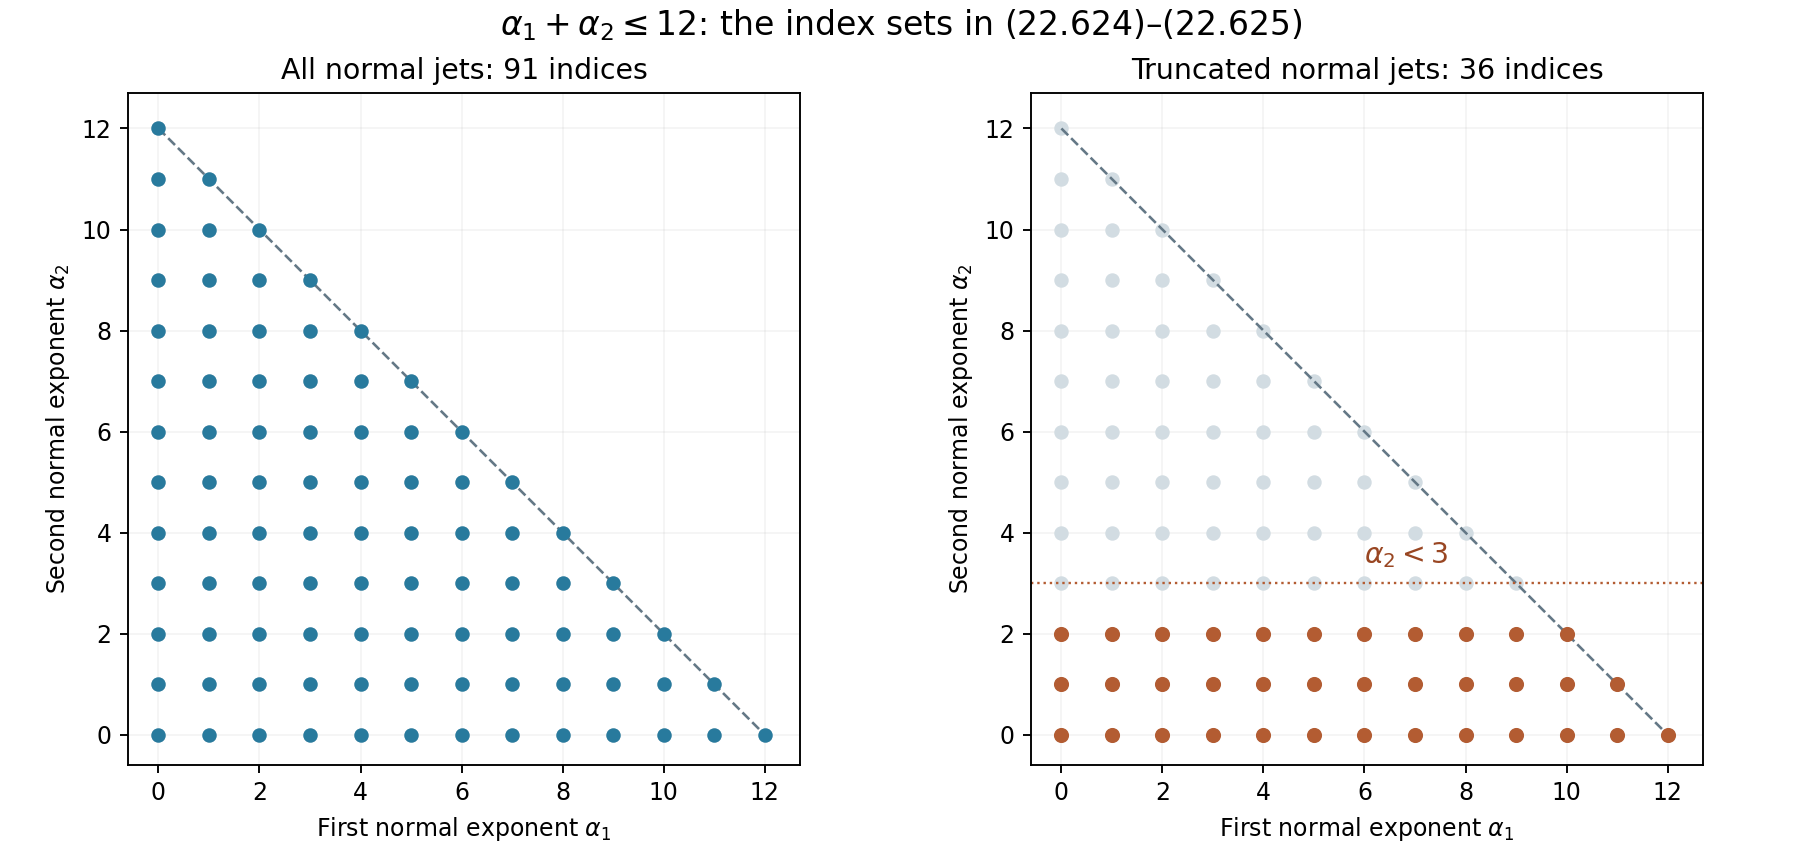
\includegraphics[keepaspectratio,alt={Full and truncated normal-jet index sets}]{../verification/lesson22/elliptic-sampling-ranks.png}}
\par\smallskip
\begin{flushleft}\small
\emph{Figure 22.18. The normal indices for \(N=12\): all 91 pairs on the
left, and the 36 pairs with \(\alpha_2<3\) on the right. These are
finite examples of the sets in Proposition 22.211; their exact counts
are given in Exercise 22.217.}
\end{flushleft}
\end{minipage}\par\medskip


The auxiliary-section method and its two sampling patterns are developed
in S. David,
\href{https://smf.emath.fr/system/files/filepdf/MSMF_1995_2_62__1_0.pdf}{\emph{Minorations
de formes linéaires de logarithmes elliptiques}}, Sections 5--7.

\subsection{The numerical elliptic logarithm
bound}\label{the-numerical-elliptic-logarithm-bound}

Throughout this section the parameters have the meaning of Propositions
22.203--205 and 22.211--216. In particular, all retained elliptic
logarithms are nonzero. Put \(B_g=\mathfrak b_g\),
\(V_g=\mathfrak v_g\), and \(E_g=\mathfrak e_g\), with the values in
(22.626)--(22.627). The letter \(E=\exp\ell\) continues to denote the
analytic parameter; it is distinct from \(E_g\).

\subsubsection{Lemma 22.218. Logarithmic and factorial
budgets}\label{lemma-22.218.-logarithmic-and-factorial-budgets}

The parameters satisfy \[
 \log U_0\le B_gL,
 \qquad d\log\mathcal M\le V_gU_0,
 \qquad \frac{5^g}{c_5}<\frac1{10^{13}n^4}.
 \tag{22.647}
\] For the bounded-product denominator of Proposition 22.168, \[
 \Delta_N(a)\mid N!,\qquad
 \log\Delta_N(a)\le N\log\max(1,N).
 \tag{22.648}
\] The last expression is zero when \(N=0\).

\textbf{Proof.} The proof of (22.629), before its final multiplication
by \(D\), gives \(\log U_0\le\log c_5+(4g+4)L\le B_gL\). Hence
\(d\log\mathcal M\le D(nB_g+g\log3+\log2)L\), and \(\Theta\ge c_4\)
proves the second assertion. The lower bound for \(c_5\) in Lemma 22.212
gives \[
 \frac{c_5}{5^g}>
 \frac{c_4^{2g+1}}{75^g n^{2g}}
 =\frac{c_4^3}{75n^2}
      \left(\frac{c_4^2}{75n^2}\right)^{g-1}
 >10^{13}n^4.
\] For positive integers \(a_1,\ldots,a_k\) with sum \(s\le N\), the
product \(a_1\cdots a_k\) divides \(s!\): indeed
\(s!/(a_1!\cdots a_k!)\) and every \((a_i-1)!\) are integers. Thus it
divides \(N!\). Taking the least common multiple proves (22.648), and
\(N!\le\max(1,N)^N\) gives its logarithmic form. \(\square\)

\subsubsection{Proposition 22.219. Repeated cosets and a sharper
periodic
basis}\label{proposition-22.219.-repeated-cosets-and-a-sharper-periodic-basis}

Partition the sampling cases by \(Q=S\) and \(Q<S\). In the second case
use \[
 S_1=2nS,\qquad T_1=\lfloor\Theta/Z_g\rfloor.
 \tag{22.649}
\] All total orders at most \(2nT\), with last normal exponent less than
\(T_1\), at \(sp\), \(0\le s<S_1\), have complex rank at most
\(\kappa\mathcal M/(2J_g)\). Moreover, writing \(j=\dim B_*\), \[
 \deg B_*\le\kappa2^g n!3^g U_0(Db)^j
                 \le e^{K_g'L},\qquad
 K_g'=\log(\kappa2^g n!3^g)+B_g+g.
 \tag{22.650}
\] Define \[
 \begin{split}
 P_g'&=K_g'+7g+3+2g\log2+\log(2nc_4),\\
 C_g'&=P_g'+3+
  \log\left(g^{3/2}\{g+2n(1+g^{3/2})\}\right).
 \end{split}
 \tag{22.651}
\] If \(0<|\Lambda|<\tfrac12e^{-P_g'DL}\), a basis
\(f=(e'_1,\ldots,e'_{g-1},w)\) exists, with the first \(j\) directions
in \(\operatorname{Lie}B_*\), and \[
 |w_g|\ge e^{-P_g'DL}/(2n).
 \tag{22.652}
\] Conversion of divided jets through order \(nT\) between \(f\) and the
graph directions costs at most \(e^{nC_g'U_0}\), in either direction.

\textbf{Proof.} When \(Q<S\), the coset of \(p\) has order exactly
\(Q\), so every sample lies in these same \(Q\) cosets. Use \(c/Q=1\) in
(22.620), together with (22.625). The rank ratio is at most
\(\kappa q/(2n2^j j!J_g)\le\kappa/(2J_g)\), since \(q=g-j\le g<n\). Also
\(T_1\le T\).

Set \(t_{\min}=c_7U_0/(DS^2v_1)\). Homogeneity and the extremal equality
give \[
 \deg B_*\le
 \kappa2^g n!3^g t_0
       \left(\frac{c_7L}{S^2}\right)^q
       \frac{v_1^j}{\prod_i v_i}.
\] By (22.604), \(c_7L/S^2<v_g\). Since every \(v_i\ge v_g\ge1\) and
\(v_1\le Db\), the remaining factor is at most \((v_1/v_g)^j\le(Db)^j\).
Now use \(t_0\le U_0\), (22.647), and \(\log(Db)\le L\). This proves
(22.650). There is a positive multiple \(Qp\) in the subgroup, with
\(Q<S\). Apply the lattice argument (22.642) and then the proof of
Corollary 22.216, using (22.650) in place of (22.641). This gives
exactly (22.651)--(22.652) and the stated change-of-basis bound.
\(\square\)

\subsubsection{Lemma 22.220. Centered interpolation with a small jet
term}\label{lemma-22.220.-centered-interpolation-with-a-small-jet-term}

Let \(s\ge100\), \(t\ge1\) be integers. Suppose the nodes
\(0,\ldots,s-1\) lie in \(|z-c|\le b_0\), put \(\Delta=X+b_0\ge s\), and
assume \(R\ge2X\), \(R>b_0\). For a function holomorphic near
\(|z-c|\le R\), set \(M_R=\max_{|z-c|\le R}|F(z)|\) and
\(\eta=\max_{h<s,m<t}|F^{(m)}(h)/m!|\). Then \[
 \max_{|z-c|\le X}|F(z)|
 \le2M_R\left(\frac{\Delta}{R-b_0}\right)^{st}
       +\eta\left(\frac{12\Delta}{s}\right)^{st}.
 \tag{22.653}
\]

\textbf{Proof.} Use the same Hermite polynomial and contour identity as
(22.391)--(22.392), with the contour centered at \(c\). The product of
the node factors is at most \(\Delta^{st}\) on the inner disc and at
least \((R-b_0)^{st}\) on the contour. The Cauchy prefactor is at most
two. The coefficient estimate (22.393) gives \[
 |H(z)|\le
 \eta s t^2\Delta^{st-1}2^{st}(2e/s)^{t(s-1)}
 \le\eta\left(\frac{4e\Delta}{s}\right)^{st}
                   t^2s^t.
 \tag{22.654}
\] The second inequality uses \(s/\Delta\le1\) and \((2e)^{-t}\le1\).
Now \(2\log t\le t\), and \((1+\log s)/s\le(1+\log100)/100<3/50\), since
\(s\mapsto(1+\log s)/s\) decreases for \(s>1\). Therefore
\(t^2s^t\le e^{3st/50}\). Finally \(e<11/4\) and
\(e^{3/50}\le(1-3/50)^{-1}=50/47\) show that \(4e e^{3/50}<12\).
Combining the two bounds proves (22.653). \(\square\)

\subsubsection{Proposition 22.221. The arithmetic lower bound at the
target
nodes}\label{proposition-22.221.-the-arithmetic-lower-bound-at-the-target-nodes}

For a polynomial in the long Weierstrass coordinates, put \[
 \mathcal A_g=V_g+
 \frac{n+\log(n^2c_4)+2}{c_6}
 +g c_7(2n^2+2)
 +n\left[\log8+\frac g4(1+\log4)+B_g+\log n\right].
 \tag{22.655}
\] Suppose \(d h_c(P)\le H_PU_0\). At an integer node
\(0\le s\le n(S-1)\), let \(f_\nu\ne0\) be a coefficient of the first
nonzero homogeneous Taylor term of the entire pullback in the graph
directions, of degree \(N\le nT\). Then \[
 \log|f_\nu|\ge-(H_P+\mathcal A_g)U_0.
 \tag{22.656}
\]

\textbf{Proof.} In each elliptic block, the short-coordinate lift is
\((\Phi_{L,1},\Phi_{L,2}/2,\Phi_{L,0})\). The corresponding polynomial
has coefficient height at most \(h_c(P)+\sum_iL_i\log2\), by
substitution, and the same number of monomials. Apply Propositions
22.199--201 over the generated field of degree \(d\). Retain the curve
bound \(\mu_E\le g(h+\log4)/4\) from (22.582), instead of replacing the
curve heights by the point budgets. The remaining point and lift terms
are bounded by \(\sum_iL_i(2s^2+48)v_i\), as in (22.593).

The monomial-count contribution is at most \(V_gU_0\), by (22.647). The
additive contribution is bounded by \(L_0d\{nb+\log(n\max(1,s))\}\),
hence by the second term of (22.655) times \(U_0\); use
\(\log(n^2S)\le\log(n^2c_4)+2R\). The point terms and the
coordinate-scaling term together are at most \(g c_7(2n^2+2)U_0\), since
\(d\le D\), \(v_i\ge1\), and \(S^2>49\). Finally (22.648),
\(N\le nU_0/(DL)\), and (22.647) give
\(\log\Delta_N(L_0)\le N(B_gL+\log n)\). Together with \(\log8+\mu_E\),
this is bounded by the last term of (22.655) times \(U_0/d\). These are
all the terms in the first-jet estimate, proving (22.656), including
\(N=0\). \(\square\)

\subsubsection{Proposition 22.222. Constants for the auxiliary section
and its
growth}\label{proposition-22.222.-constants-for-the-auxiliary-section-and-its-growth}

Define \[
 D_g=3+\log2+\tfrac32\log g,
 \qquad M_g=\mathfrak m_g+V_g+\frac{\log5}{c_4}.
 \tag{22.657}
\] Use subscripts \(N\) and \(P\) for the cases \(Q=S\) and \(Q<S\),
respectively. Set \[
 \begin{split}
 G_N&=V_g+\frac{\log(4nc_4)+3}{c_6}
       +g c_7\{(1+\lambda)e^2n^2+1\}+nD_g,\\
 G_P&=V_g+\frac{\log(8nc_4)+3}{c_6}
       +g c_7\{(1+\lambda)(2e+1)^2n^2+1\}+nD_g.
 \end{split}
 \tag{22.658}
\] The other constants are specified by the following table:

{\def\LTcaptype{none} % do not increment counter
\begin{longtable}[]{@{}
  >{\raggedright\arraybackslash}p{(\linewidth - 4\tabcolsep) * \real{0.2727}}
  >{\raggedleft\arraybackslash}p{(\linewidth - 4\tabcolsep) * \real{0.3636}}
  >{\raggedleft\arraybackslash}p{(\linewidth - 4\tabcolsep) * \real{0.3636}}@{}}
\toprule\noalign{}
\begin{minipage}[b]{\linewidth}\raggedright
Constant
\end{minipage} & \begin{minipage}[b]{\linewidth}\raggedleft
Case \(N\)
\end{minipage} & \begin{minipage}[b]{\linewidth}\raggedleft
Case \(P\)
\end{minipage} \\
\midrule\noalign{}
\endhead
\bottomrule\noalign{}
\endlastfoot
\(K_\bullet\) & \(\tfrac32n\log g\) & \(nC_g'\) \\
\(W_\bullet\) & \(n(3+\tfrac32\log g+2\log2)+\log2/c_4\) &
\(\log2/c_4\) \\
\(I_\bullet\) & \(8n^2A_g\log(13nZ_g)\) & \(16n^2A_g\log13\) \\
\(F_\bullet\) & \(7n^2A_g\) & \(11n^2A_g\) \\
\end{longtable}
}

Also put \[
 \begin{split}
 Q_g&=V_g+\frac{B_g}{c_4}+
       \frac{\log(8nc_4)+2}{c_6}
       +g c_7(12n^2+1)+2nD_g,\\
 Z_g'&=\frac{\log(2nc_4)+2}{c_4},\qquad
 r_N=\frac{2\kappa}{J_g-2\kappa},\quad
 r_P=\frac{\kappa}{J_g-\kappa}.
 \end{split}
 \tag{22.659}
\] For either subscript define \[
 \begin{split}
 a_\bullet&=
 \frac{r_\bullet M_g+E_g+\mathcal A_g+W_\bullet+
                         I_\bullet+K_\bullet+2}{1-r_\bullet},\\
 H_\bullet&=r_\bullet(a_\bullet+M_g)+E_g,\\
 L_\bullet&=a_\bullet+H_\bullet+Q_g+Z_g'+1+
                          \frac{P_g'+\log2}{c_4}.
 \end{split}
 \tag{22.660}
\] All denominators here are positive. If
\(0<|\Lambda|<e^{-L_\bullet U_0}\), there is a nonzero section \(P\)
with \[
 d h_c(P)\le H_\bullet U_0,
 \qquad |\text{sampled divided jet at }su|
                                      \le e^{-a_\bullet U_0}.
 \tag{22.661}
\] The sample orders in case \(N\) are those of Proposition 22.211; in
case \(P\) they are those of Proposition 22.219.

\textbf{Proof.} The assumption implies \(|\Lambda|<1\) and, when needed,
the basis condition in Proposition 22.219, because \(U_0\ge c_4DL\). The
matrix ranks divided by their numbers \(d\mathcal M\) of integer
unknowns are at most \(\kappa/(dJ_g)\) and \(\kappa/(2dJ_g)\). In the
pigeonhole argument, use \(2\eta/(1-2\eta)\), rather than the upper
bound \(4\eta\), as the multiplier of \(p+m+\log(1+4\nu)\). Inequality
(22.386) still holds, with equality permitted;
\(\lfloor e^\delta\rfloor+1>e^\delta\) supplies the strict box
inequality. After multiplication by \(d\), these multipliers are at most
\(r_N,r_P\), respectively. Propositions 22.212--214 now give (22.661).

Here are growth estimates used below. For a unitary multi-index
\(\alpha\), \(|\alpha|\le nT\), the function
\(D_{e'}^\alpha F(zw)/\alpha!\) has norm at most \(e^{(H_N+G_N)U_0}\) on
\(|z|\le EnS\). In case \(P\), use only the first \(g-1\) directions;
its norm on \(|z-(nS-1/2)|\le2EnS\) is at most \(e^{(H_P+G_P)U_0}\).

To verify these assertions, retain the factor \(e^{1-\ell}\) in the
analytic parameter condition:
\(|u_i/\omega_i|\le e^{1-\ell}\sqrt{Dv_i y_i/(3\pi)}\). On the two discs
the normalized center coordinates have modulus at most
\(enS\sqrt{Dv_i y_i/(3\pi)}\) and \((2e+1)nS\sqrt{Dv_i y_i/(3\pi)}\),
respectively. If this modulus is \(A\), the scaled Cauchy polydisc from
(22.631) changes it by at most one. Completing the square gives \[
 \log(3.33)+\tfrac34Dh_i+
 3\pi\left(\frac{(A+1)^2}{y_i}+A+1+\frac{y_i}{4}\right)
 \le(1+\lambda)\frac{3\pi A^2}{y_i}
                         +26(1+\lambda^{-1})Dv_i.
 \tag{22.662}
\] Indeed the linear term \(A(2/y_i+1)\) is at most
\(\lambda A^2/y_i+(1/y_i+1+y_i/4)/\lambda\); use \(y_i>6/7\),
\(y_i\le Dh\le Dv_i\), and \(\pi<22/7\) for the remaining constants. We
have \(S^2>26(1+100g^2)\), by (22.605). Multiplying by the degrees
proves the elliptic terms in (22.658). The additive factors are at most
\((4EnS)^{t_0}\) and \((8EnS)^{t_0}\), respectively. Their logarithms
give the displayed terms divided by \(c_6\). Cauchy's divided-derivative
cost is at most \(nD_gU_0\), and the monomial count contributes
\(V_gU_0\).

Finally, for every sampled jet, and for every canonical jet of order at
most \(nT\), the change between \(su\) and \(sw\) is at most \[
 e^{-(a_\bullet+1)U_0}.
 \tag{22.663}
\] For detail, differentiate in the additive coordinate along the
segment. This multiplies polynomial coefficients by at most \(L_0\); its
logarithm is at most \(B_gL\). The monomial, additive, elliptic and
directional estimates are then precisely the four contributions to
\(Q_g\). Thus the differentiated jet is at most
\(e^{(H_\bullet+Q_g)U_0}\). The segment has length \(s|\Lambda|\), with
\(\log(2nS)\le Z_g'U_0\). The definition of \(L_\bullet\) proves
(22.663) by integration along this segment. \(\square\)

\subsubsection{Proposition 22.223. Extrapolation in the two
cases}\label{proposition-22.223.-extrapolation-in-the-two-cases}

For the section of Proposition 22.222, every divided graph jet of order
at most \(nT\) at \(su\), \(0\le s\le n(S-1)\), has modulus at most \[
 2e^{(H_\bullet+G_\bullet-F_\bullet+K_\bullet)U_0}
 +e^{(-a_\bullet+W_\bullet+I_\bullet+K_\bullet)U_0}
 +e^{-(a_\bullet+1)U_0}.
 \tag{22.664}
\]

\textbf{Proof.} Each real quantity whose floor defines \(S,T,S_0,T_1\)
exceeds 100. This follows from \(c_4>10^5n^2\), \(\Theta\ge c_4\), and
\(S/Z_g\ge4nA_g>100\). Consequently each floor is at least \(99/100\) of
its argument. All interpolation node counts are at least 100.

In case \(N\), fix \(|\alpha|\le nT\) and apply Lemma 22.220 to
\(G(z)=D_{e'}^\alpha F(zw)/\alpha!\), with \[
 s=S_0,\quad t=nT,\quad c=0,\quad b_0=S_0,
 \quad X=nS,\quad R=EnS.
 \tag{22.665}
\] Its derivatives through order \(nT-1\) use only sampled jets through
order \(2nT-1\), by (22.486). The sum of the coefficients in that
formula is at most \(2^{2nT}\max(1,\sum|w_j|)^{nT}\), and
\(\sum|w_j|\le g^{3/2}e^{3DL}\). Combining this with (22.663) gives
\(\eta\le e^{(-a_N+W_N)U_0}\).

Put \(x_0=S_0/(nS)\le1/(nZ_g)<1/100\). Then \[
 \frac{\Delta}{R-b_0}=
 \frac{1+x_0}{E-x_0}
 \le E^{-1}\frac{101}{99}
 <e^{-19\ell/20},
 \qquad \frac{12\Delta}{S_0}<13nZ_g.
 \tag{22.666}
\] The second inequality uses \(S_0\ge(99/100)S/Z_g\). The norm estimate
from Proposition 22.222 and \(8(99/100)^3(19/20)>7\) now give \[
 \frac{19}{20}S_0nT\ell>7n^2A_gU_0,
 \qquad S_0nT\log(13nZ_g)\le I_NU_0.
 \tag{22.667}
\] This proves the first two terms of (22.664) in the unitary basis at
\(sw\). Conversion to the graph basis costs \(e^{K_NU_0}\).

In case \(P\), write \(f=(f',w)\), fix \(|\alpha'|\le nT\), and apply
Lemma 22.220 to \(G(z)=D_{f'}^{\alpha'}F(zw)/\alpha'!\), using \[
 s=2nS,\quad t=T_1,\quad c=nS-\tfrac12,
 \quad b_0=nS,\quad X=nS+1,\quad R=2EnS.
 \tag{22.668}
\] Its derivatives of order less than \(T_1\) are exactly the sampled
divided \(f\)-jets. Their total orders are at most \(nT+T_1-1\le2nT-1\).
Thus \(\eta\le e^{(-a_P+W_P)U_0}\). Here \(1/(nS)\le\lambda\le1/100\),
so \[
 \frac{\Delta}{R-b_0}
 =\frac{2+1/(nS)}{2E-1}
 \le e^{-3\ell/4},\qquad
 \frac{12\Delta}{2nS}<13.
 \tag{22.669}
\] For the first inequality, use \(e>8/3\) and
\((2+1/100)/(2-e^{-1})<5/4<e^{1/4}\). Moreover \(16(99/100)^2(3/4)>11\),
whence \[
 \frac34(2nS)T_1\ell>11n^2A_gU_0,
 \qquad (2nS)T_1\log13\le I_PU_0.
 \tag{22.670}
\] This bounds \(G\) on the entire inner disc. The unit circle about any
target integer lies in that disc. Cauchy's coefficient formula therefore
bounds every \(G^{(m)}(s)/m!\), including all remaining last exponents
with \(|\alpha'|+m\le nT\). This includes \(g=1\), when \(\alpha'\) is
empty. Convert the basis using Proposition 22.219, with cost
\(e^{K_PU_0}\). Finally (22.663), in the graph directions, returns from
\(sw\) to \(su\) in both cases. \(\square\)

\subsubsection{Lemma 22.224. The numerical
comparison}\label{lemma-22.224.-the-numerical-comparison}

For every integer \(g\ge1\), and in both cases, \[
 F_\bullet>2H_\bullet+G_\bullet+K_\bullet+
                    \mathcal A_g+2,
 \qquad
 c_5L_\bullet+5^g<C(g),
 \tag{22.671}
\] where \[
 C(g)=2.9\cdot10^6\,10^{6g}\,4^{2g^2}
                   (g+1)^{2g^2+9g+123/10}.
 \tag{22.672}
\]

\textbf{Proof.} We give an elementary estimate for \(g\ge10000\) and an
exact finite certificate for the remaining integers. For the first range
put \(x=\log n\), \(y=\log(4n)\), and \(\Sigma=n^2A_g\). The definitions
imply \[
 \begin{gathered}
 x>9,\quad \log y\le x/3,\quad
 gy\le A_g\le1.001gy,\quad
 9.3ny<J_g<11ny,\quad \lambda\le10^{-10},\\
 \log c_4\le gy+4x+2\log y+4.51\le gy+6x,
 \quad B_g\le2.01nA_g,\quad
 \log(13nZ_g)\le1.001gy.
 \end{gathered}
 \tag{22.673}
\] Here \(5x+15\le(20/3)x\le.001gy\) proves the bound for \(A_g\). In
the formula for \(J_g\), its leading coefficient lies between 9.3 and
10, while \(56x+54\le62x<ny\). Substitution in the formula for \(c_4\)
proves its logarithmic bound, since
\(\log(88\cdot1.001)+\log(1+10^{-10})<4.51\). The function
\(x/3-\log(x+\log4)\) is positive at 9 and increasing thereafter,
proving the bound for \(\log y\). For \(B_g\), discard the negative
terms \(-\log(n!)\) and \(-g\log(6c_7)\) in \(\log c_5\), and use
\(\log c_6=x+g\log2\). The resulting upper bound is
\(2g^2y+gy+12gx+4.7g+7x+4\), which is less than \(2.01ngy\). Finally
\(\log(13nZ_g)=\log c_4+\log(13/8)-\log A_g\) gives the last assertion
of (22.673).

The following rational bounds now follow by substitution:

{\def\LTcaptype{none} % do not increment counter
\begin{longtable}[]{@{}lr@{}}
\toprule\noalign{}
Quantity divided by \(\Sigma\) & Upper bound \\
\midrule\noalign{}
\endhead
\bottomrule\noalign{}
\endlastfoot
\(M_g\), \(Q_g\) & \(1.16\) \\
\(\mathcal A_g\) & \(2.21\) \\
\(G_N\), \(G_P\) & \(0.70\), \(4\) \\
\(K_N\), \(K_P\) & \(0.001\), \(2.02\) \\
\(W_N,W_P,Z_g',2,(P_g'+\log2)/c_4\) & \(0.001\) each \\
\(E_g\) & \(10^{-20}\) \\
\end{longtable}
}

To verify the entries explicitly, use \(g c_7=4A_g/(13+4e^2)\),
\(42.5<13+4e^2<43\), and \(2.718<e<2.719\). The leading terms in
\(M_g,Q_g\), \(\mathcal A_g\), \(G_N\), and \(G_P\), after division by
\(\Sigma\), are respectively at most \(48/42.5\),
\(2.01+8(1+n^{-2})/42.5\), \((1+10^{-10})4(2.719)^2/(13+4(2.719)^2)\),
and \((1+10^{-10})4(2(2.719)+1)^2/42.5\). The remaining terms in each of
these rows total less than \(1/1000\): use \(V_g/\Sigma<3/c_4\),
\(c_6\ge ng^2\), \(D_g\le2x\), and \(n g(1+\log4)/(4\Sigma)<0.6/(ny)\).
The bound for the periodic basis follows from \(P_g'\le B_g+5gy\) and
\(C_g'\le P_g'+4x+5\). These inequalities follow by using
\(\log(n!)\le n\log n\) in (22.651). The bounds involving \(E_g\) and
\(c_4^{-1}\) follow directly from (22.605) and (22.647).

Also \(r_N<.216/(ny)\), \(r_P<.108/(ny)\), and
\((1-r_\bullet)^{-1}<1.00001\). From (22.660), equivalently, \[
 H_\bullet=
 \frac{r_\bullet}{1-r_\bullet}
  (M_g+\mathcal A_g+W_\bullet+I_\bullet+K_\bullet+2)
 +\frac{E_g}{1-r_\bullet}.
 \tag{22.674}
\] Use \(I_N/\Sigma\le8.008gy\), \(I_P/\Sigma<41.6\), and \(ny>90000\).
This gives \(H_N/\Sigma<1.74\) and \(H_P/\Sigma<.001\). The margins in
the first inequality of (22.671), divided by \(\Sigma\), are therefore
greater than \(7-3.48-.70-.001-2.21-.001>1/2\) and
\(11-.002-4-2.02-2.21-.001>2\).

For the second inequality, the same bounds and
\(a_\bullet=H_\bullet+\mathcal A_g+W_\bullet+
I_\bullet+K_\bullet+2\) give \(L_\bullet<9gy\Sigma<10n^4y^2\). Integral
comparison gives \(\log(n!)\ge n\log n-n+1\), and \(6c_7>24y/43\), with
\(\log(43/24)<.6\). Inserting the first bound for \(\log c_4\) in
(22.673) into \(\log c_5\) therefore yields \[
 \log c_5<2g^2\log4+(2g^2+8g+4)x
                 +(3g+2)\log y+12.72g+4.51.
 \tag{22.675}
\] Here \(\log8<2.1\) suffices for the constant 12.72. On the other hand
\(\log10>9/4\) and \(\log(2.9\cdot10^6)>14\). Thus
\(\log C(g)-\log c_5>g/2+7x\), using \(\log y\le x/3\). Since \(y^2<n\)
for \(x>9\), we obtain \(L_\bullet+5^g/c_5<11n^5<e^{g/2}n^7<C(g)/c_5\).
This proves both inequalities for every \(g\ge10000\).

For \(1\le g\le9999\), the
\href{verification/lesson22/elliptic-numerical-extrapolation-check.py}{integer
interval certificate} verifies the stronger bounds \[
\begin{gathered}
 \frac{F_N-2H_N-G_N-K_N-\mathcal A_g-2}{\Sigma}>\frac12,\\
 \frac{F_P-2H_P-G_P-K_P-\mathcal A_g-2}{\Sigma}>2,\\
 \log\frac{c_5L_\bullet+5^g}{C(g)}<-\frac1{25}.
\end{gathered}
\tag{22.676}
\] Here is the complete enclosure procedure. An interval is a pair of
integers divided by \(2^{128}\); addition is exact, and multiplication
and division round the extremal endpoint quotients outwards using
integer division. Square roots use the integer square root of the
endpoint times \(2^{128}\). To enclose a logarithm, reduce its argument
to \(2^k m\), \(1\le m\le2\), and use
\(\log m=2\sum_{j\ge0}z^{2j+1}/(2j+1)\), \(z=(m-1)/(m+1)\). After 64
terms, the remainder is at most \(2z^{129}/(129(1-z^2))<2^{-128}\); the
slightly enlarged endpoint also has \(z<1/2\). The same series at
\(z=1/3\) encloses \(\log2\). The sum \(\sum_{k=0}^{64}1/k!\), with
remainder less than \(2/65!<2^{-128}\), encloses \(e\). These remainder
bounds follow by summing geometric series; the logarithmic identity
follows by integrating one.

The certificate substitutes these intervals in (22.657)--(22.672) for
each of the 9,999 integers, maintaining \(\log(n!)=\sum_{j=1}^n\log j\).
It encloses \(c_4^{-1}\) by \([0,(10^5n^2)^{-1}]\) and \(5^g/c_5\) by
\([0,(10^{13}n^4)^{-1}]\), as proved above. For each of the two cases it
compares the lower endpoint of the first margin and the upper endpoint
of the last logarithm with the rational endpoints in (22.676). All
39,996 comparisons pass. The operations and remainder bounds just given
establish that each interval contains the exact expression; thus these
finite comparisons, together with the preceding infinite-range proof,
prove (22.671). \(\square\)

\subsubsection{Theorem 22.225. The explicit bound for a nonzero elliptic
form}\label{theorem-22.225.-the-explicit-bound-for-a-nonzero-elliptic-form}

Let the nonzero elliptic logarithms \(u_1,\ldots,u_g\), their algebraic
exponential points, the curves, field degree \(D\), heights \(h,v_i\),
and analytic parameter \(\ell=\log E\) satisfy (22.598). Let
\(u_0,\beta_1,\ldots,\beta_g\) belong to that field, and suppose
\(b\ge\max\{eh,h(u_0),h(\beta_1),\ldots,h(\beta_g)\}\). If
\(\Lambda=u_0-\sum_i\beta_i u_i\ne0\), then \[
 \log|\Lambda|>
 -C(g)D^{2g+2}(b+\log D+\ell)
       (\log b+h+\log D+\ell)^{g+1}
       \left(\prod_i v_i\right)\ell^{-2g-1},
 \tag{22.677}
\] with the explicit constant (22.672).

\textbf{Proof.} First assume that every \(\beta_i\ne0\) and the
coefficients are normalized as in Lemma 22.212. In the appropriate
sampling case, suppose \(0<|\Lambda|<e^{-L_\bullet U_0}\), and construct
the section in Proposition 22.222. Proposition 22.208 supplies a nonzero
graph jet at a target node. Choose the least nonzero homogeneous degree
at that node. Its coefficient \(f_\nu\) satisfies (22.656).

By definition of \(a_\bullet\), the second exponent in (22.664) equals
\(-(H_\bullet+\mathcal A_g+2)U_0\). The first inequality of (22.671)
makes the first exponent smaller than that value. The last exponent is
also no larger. Hence \[
 |f_\nu|<4e^{-(H_\bullet+\mathcal A_g+2)U_0}
              <e^{-(H_\bullet+\mathcal A_g)U_0},
 \tag{22.678}
\] because \(U_0\ge1\) and \(e^2>4\). This contradicts (22.656). Thus
\(\log|\Lambda|\ge-L_\bullet U_0\) for normalized coefficients.

For general coefficients choose a member \(x\) of
\((u_0,\beta_1,\ldots,\beta_g)\) with largest complex absolute value and
divide by it. Lemma 22.141 gives absolute values at most one and tuple
height at most \(nb\). Also \(h(x)\le b\), so \(\log|x|\ge-Db\). All
elliptic parameters remain unchanged. By (22.628), \[
 Db\le\frac{5^g}{c_5}U_0,
 \qquad
 \log|\Lambda|\ge-(L_\bullet+5^g/c_5)U_0.
 \tag{22.679}
\] The second inequality of (22.671) and the definition of \(U_0\) now
give the strict inequality (22.677).

If exactly \(m\) coefficients \(\beta_i\) are nonzero, with \(0<m<g\),
apply the proved case to those terms, reordered by their height budgets.
Their curve-height maximum is at most \(h\). For every omitted index,
(22.599) gives \(D^2Lv_i/\ell^2\ge D/5\ge1/5\). Thus the parameter
factor in dimension \(g\), without \(C(g)\), is at least \(5^{-(g-m)}\)
times the factor in dimension \(m\). Formula (22.672) gives
\(C(g)/C(m)>5^{g-m}\): each successive ratio exceeds \(10^6\). This
proves (22.677) with its original dimension. If all \(\beta_i\) vanish,
the product formula gives \(\log|u_0|\ge-Db\). The right-hand magnitude
in (22.677) is greater than \(C(g)D^3b/5^g>Db\), by (22.628), so the
conclusion holds in this case too. \(\square\)

Terms with zero elliptic logarithm are omitted before choosing the
dimension and parameters in (22.598).

\subsubsection{Exercise 22.226. Centering the interpolation
contour}\label{exercise-22.226.-centering-the-interpolation-contour}

Use nodes \(0,\ldots,99\), center \(c=49.5\), \(b_0=50\), inner radius
\(X=51\), and outer radius \(R=100e\). For a common interpolation order
\(t\), give a bound from Lemma 22.220 and show that the unit circles
about \(0,24,48\) lie in the inner disc.

\textbf{Solution.} We have \(\Delta=101\), so
\(12\Delta/100=303/25<13\). Furthermore
\((2+1/50)/(2-e^{-1})<5/4<e^{1/4}\), using \(e>8/3\). Hence
\(101/(100e-50)<e^{-3/4}\), and \[
 \max_{|z-49.5|\le51}|F(z)|
       \le2M_{100e}e^{-75t}+\eta13^{100t}.
 \tag{22.680}
\] The three circles have maximal distances \(50.5,26.5,2.5\) from the
center, respectively, all less than 51. Their Cauchy integrals therefore
recover every divided derivative at these three nodes from the
inner-disc norm. \(\square\)

\begin{minipage}[t]{\linewidth}
\centering
\pandocbounded{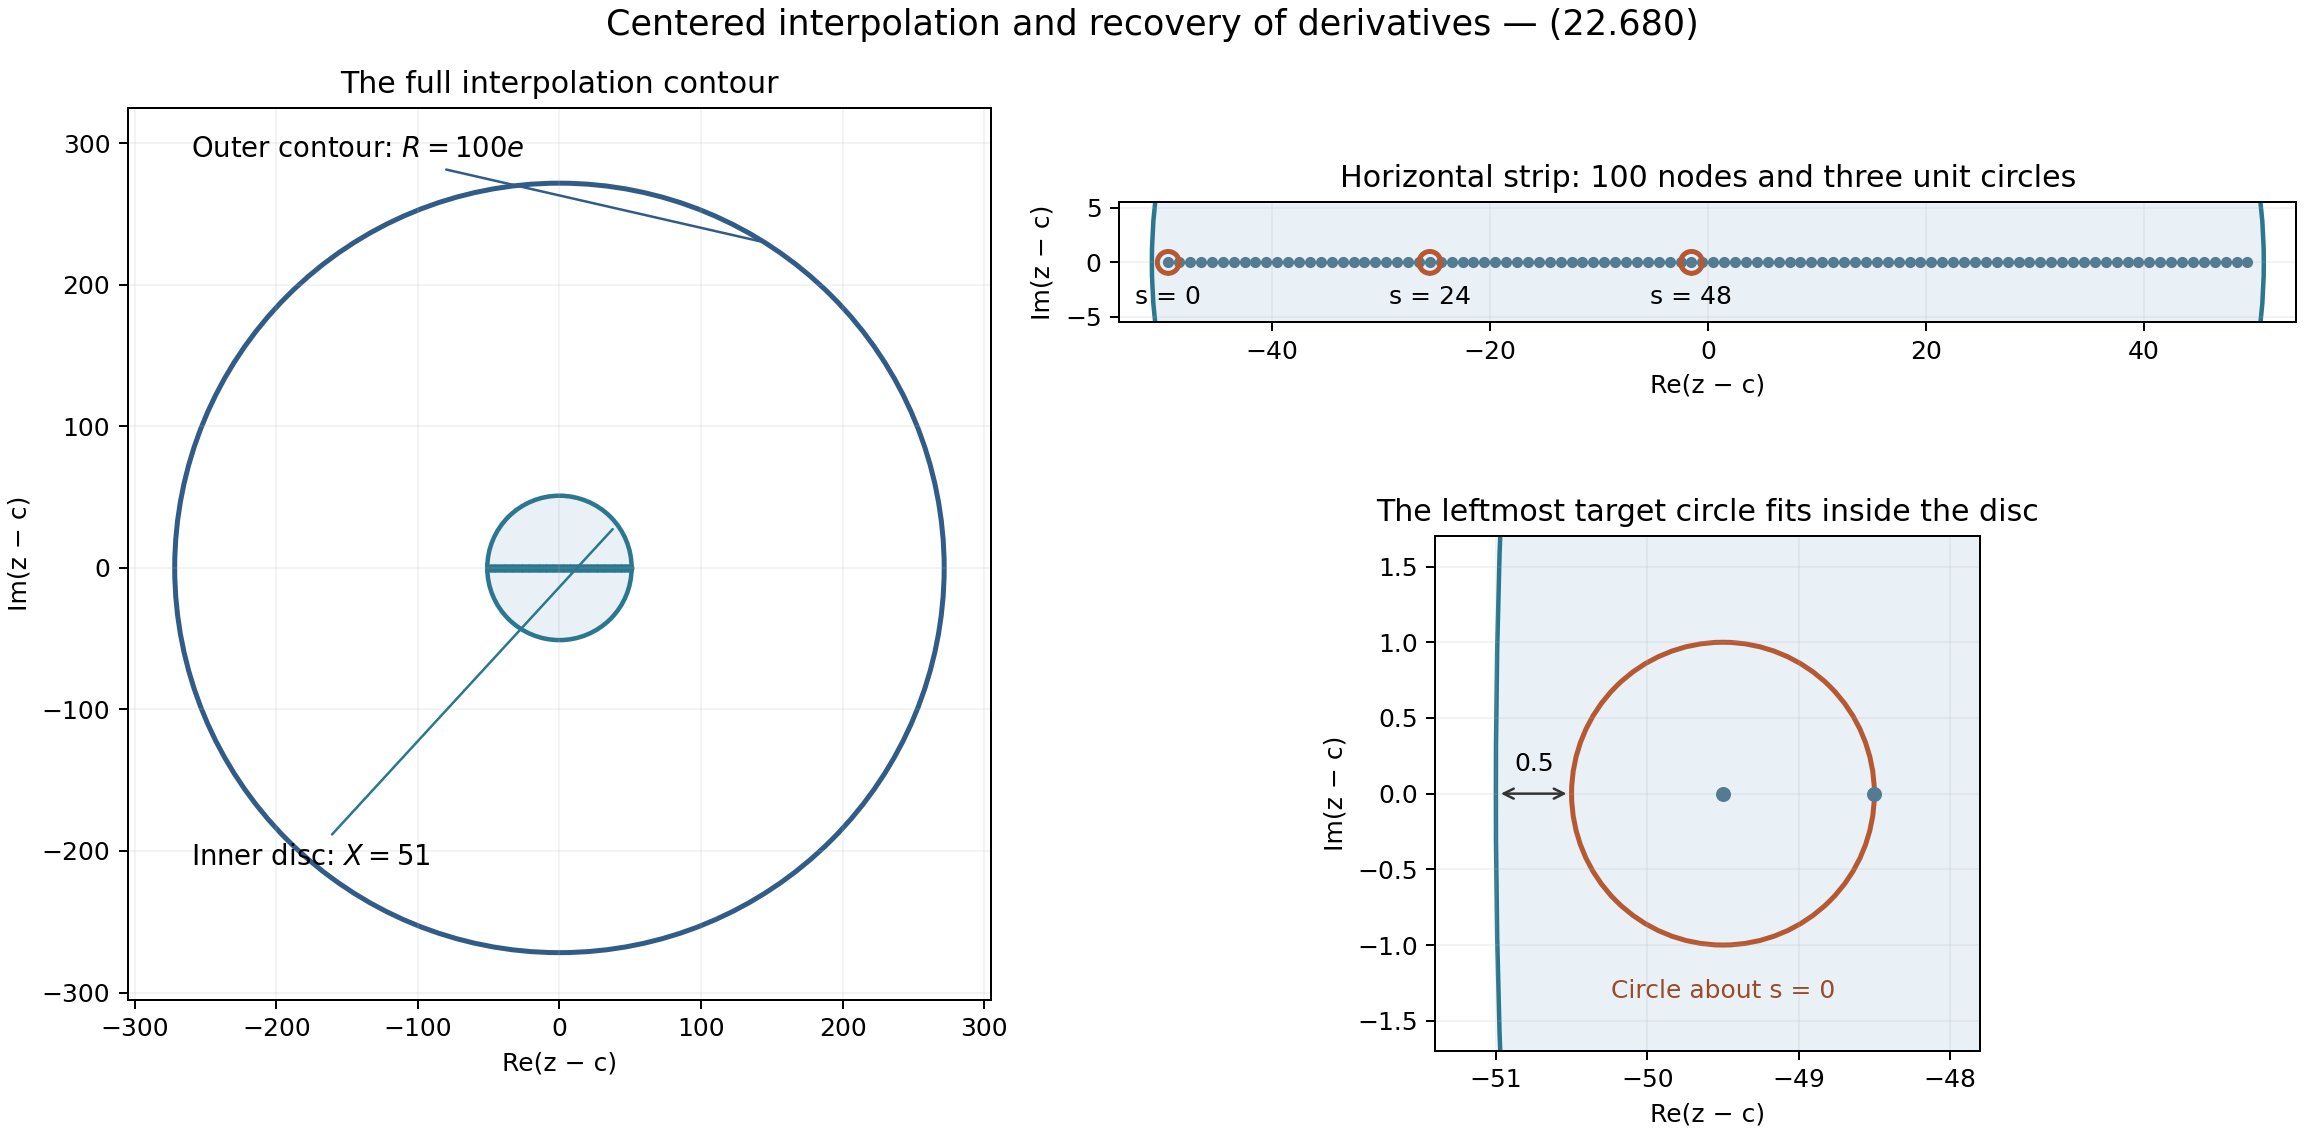
\includegraphics[keepaspectratio,alt={A centered outer interpolation contour and unit circles at three target nodes}]{../verification/lesson22/elliptic-centered-interpolation.png}}
\par\smallskip
\begin{flushleft}\small
\emph{Figure 22.19. The exact geometry of Exercise 22.226. Coordinates
are translated by \(49.5\). The upper right panel shows a horizontal
strip of the inner disc; the lower panel shows the leftmost unit circle
and its clearance of \(0.5\). The full outer contour on the left
controls the Hermite remainder.}
\end{flushleft}
\end{minipage}\par\medskip


For the elliptic auxiliary-section argument and the explicit constant,
see S. David,
\href{https://smf.emath.fr/system/files/filepdf/MSMF_1995_2_62__1_0.pdf}{\emph{Minorations
de formes linéaires de logarithmes elliptiques}}, Theorem 2.1 and
Sections 5--9.

\subsection{Integral points from elliptic
logarithms}\label{integral-points-from-elliptic-logarithms}

Let \[
 E:y^2=x^3+Ax+B=f(x),\qquad A,B\in\mathbf Z,
 \qquad 4A^3+27B^2\ne0.
\] The corresponding long model is \(Y=2y\), with invariants
\(g_2=-4A,g_3=-4B\). All canonical heights in this section are
\(q=\widehat h_3\) from (22.570). In particular, they are three times
the normalization \(\tfrac12\widehat h_x\).

The computational input is a finite torsion subgroup \(T\), a positive
integer \(t\) with \(tT=0\), and rational points \(P_1,\ldots,P_r\)
independent modulo torsion. Write \(\Gamma=T+\sum_i\mathbf ZP_i\). The
method below determines every integral point in \(\Gamma\). It
determines every integral point of \(E(\mathbf Q)\) when the equality
\(\Gamma=E(\mathbf Q)\) has also been proved. A rank computation and
independent points alone do not establish that equality.

\subsubsection{Proposition 22.227. A certified quadratic lower
bound}\label{proposition-22.227.-a-certified-quadratic-lower-bound}

The canonical pairing \[
 \langle P,Q\rangle_q
 =\tfrac12\{q(P+Q)-q(P)-q(Q)\}
 \tag{22.681}
\] is symmetric and additive in each argument. Its matrix
\(G=(\langle P_i,P_j\rangle_q)\) is positive definite, and \[
 q\left(T_0+\sum_i n_iP_i\right)=n^{\mathsf T}Gn
 \ge\lambda\sum_i n_i^2\ge\lambda N^2,
 \qquad N=\max_i|n_i|,
 \tag{22.682}
\] whenever \(T_0\in T\) and \(G-\lambda I\) is positive semidefinite. A
positive rational \(\lambda\) can be certified by finite calculations.

\textbf{Proof.} For \(M=\mathcal O_E(2O)\), the cube identity proved in
\href{https://github.com/KokunoYumeto/open-math-courses-public/blob/146dc81802e69cf262fb6cc65c1b9f74e71f4625/docs/courses/AG-GS/src/abelian-varieties.md\#4-the-theorem-of-the-cube-and-the-square}{\emph{Abelian
varieties}, Corollary 4.2} pulled back along \((P,Q,-Q)\) gives
\(m^*M\otimes d^*M\simeq p_1^*M^2\otimes p_2^*M^2\), where
\(m(P,Q)=P+Q\), \(d(P,Q)=P-Q\). Proposition 22.49 therefore bounds
\(h_x(P+Q)+h_x(P-Q)-2h_x(P)-2h_x(Q)\) independently of \((P,Q)\).
Substitute \((2^sP,2^sQ)\), divide by \(4^s\), and use (22.570). Thus
\(q\) satisfies the parallelogram identity.

Polarization gives additivity directly. Write
\(B(x,y)=(q(x+y)-q(x-y))/4\). Two parallelogram identities give
\(B(x+z,y)+B(x-z,y)=2B(x,y)\). Interchanging \(x,z\), using
\(B(z-x,y)=-B(x-z,y)\), and adding gives \(B(x+z,y)=B(x,y)+B(z,y)\).
Symmetry gives additivity in the other argument. This is (22.681), and
\(B(x,x)=q(x)\). A torsion argument has pairing zero, since a nonzero
integer multiple of that pairing is zero. Expansion proves the equality
in (22.682).

The limit defining \(q\) is nonnegative. Bounded \(q\) gives bounded
\(h_x\) by (22.567), since \(h_x\le 2q/3+B_E/3\). There are only
finitely many rational \(x=a/b\) in lowest terms with
\(\log\max(|a|,|b|)\) bounded, and at most two points above each \(x\).
This proves the required finiteness without a separate height-finiteness
theorem. In particular, \(q(P)=0\) implies that the points \(nP\) form a
finite set, by (22.573), so \(P\) is torsion.

Nonnegativity on integer vectors implies nonnegativity on rational and
then real vectors. If \(Gv=0\) for a nonzero real vector \(v\), round
\(kv\) coordinatewise to integer vectors \(a_k\). They are unbounded,
but \(a_k^{\mathsf T}Ga_k\) is bounded: the kernel term vanishes and the
rounding errors have bounded norm. Independence modulo torsion gives
infinitely many distinct points of bounded height, a contradiction. Thus
\(G\) is positive definite.

For computation, duplication and (22.567) enclose each \(q(P_i)\) and
\(q(P_i+P_j)\) in intervals of width tending to zero. Suppose a rational
symmetric matrix \(R\) satisfies \(|G_{ij}-R_{ij}|\le\epsilon\). Then \[
 x^{\mathsf T}Gx\ge x^{\mathsf T}Rx-r\epsilon\|x\|_2^2.
 \tag{22.683}
\] Indeed \((\sum|x_i|)^2\le r\sum x_i^2\), by summing the nonnegative
squares \((|x_i|-|x_j|)^2\). Rational elimination certifies positivity
of \(R-(\lambda+r\epsilon)I\): factor it as \(LDL^{\mathsf T}\) and
check that all diagonal pivots of \(D\) are positive. The resulting
expression is a sum of positive multiples of squares. Because \(G\) is
positive definite, sufficiently accurate intervals and a sufficiently
small positive rational \(\lambda\) pass this test. This proves both the
lower bound and its effective certification. \(\square\)

\subsubsection{Lemma 22.228. The real branch at
infinity}\label{lemma-22.228.-the-real-branch-at-infinity}

Choose an integer \(H\ge2\) with \(H^2\ge4|A|\) and \(H^3\ge4|B|\). Let
\(e_0\) be the largest real root of \(f\), and let \(\Omega>0\) generate
the real periods of \(dx/(2y)\). For \(x(P)\ge H\), the real logarithm
representing \(P\) is \[
 u(P)=-\operatorname{sgn}(y(P))I(x(P)),\qquad
 I(x)=\int_x^\infty\frac{ds}{2\sqrt{f(s)}},\qquad
 0<I(x)\le\sqrt{2/x}.
 \tag{22.684}
\] It lies in \((-\Omega/2,\Omega/2)\) and is nonzero. There are no real
points with \(x\le-H\). Every real point doubles into the identity
component.

\textbf{Proof.} For \(s\ge H\), \(f(s)\ge s^3-|A|s-|B|\ge s^3/2>0\); the
analogous estimate for \(s\le-H\) gives \(f(s)\le-|s|^3/2<0\).
Integration of \(s^{-3/2}/\sqrt2\) proves (22.684). The real locus
consists of the two graphs \(\pm\sqrt{f(x)}\) joined at simple roots,
together with \(O\). Its unbounded component is \(x\ge e_0\), closed by
\(O\); if three real roots occur, there is one further oval between the
other two roots. Thus its component group has order at most two, proving
the doubling assertion.

The uniformization already proved identifies the differential with
\(du\). Near \(O\), \(x=u^{-2}+O(u^2)\) and \(y=-u^{-3}+O(u)\), so its
sign gives exactly (22.684). Following the two graphs around the
unbounded component gives \[
 \Omega=2I(e_0).
 \tag{22.685}
\] The endpoint integral converges since the root is simple. The
uniformization is injective on one traversal of that component, so this
is its least positive real period. Consequently \(I(x)<\Omega/2\) for
\(x>e_0\).

These integrals admit certified approximations. For example \[
 I(x)=\int_{\sqrt{x-e_0}}^\infty
 \frac{ds}{\sqrt{s^4+3e_0s^2+3e_0^2+A}}.
 \tag{22.686}
\] The denominator is positive for \(s\ge0\): its square equals
\(f(e_0+s^2)/s^2\), with positive limiting value \(f'(e_0)\). On a
bounded interval, isolating the algebraic root and subdividing gives
upper and lower Riemann sums with arbitrarily small difference. Their
convergence follows from continuity and the positive minimum of that
denominator. The remaining tail is bounded by (22.684). This also
computes logarithms of any specified real point in the identity
component, with its sign and endpoint included. \(\square\)

\subsubsection{Proposition 22.229. A nonzero form with a Gaussian upper
bound}\label{proposition-22.229.-a-nonzero-form-with-a-gaussian-upper-bound}

Suppose \(r\ge1\). Put \(Q_i=[2t]P_i\), and choose their real logarithms
\(u_i\in(-\Omega/2,\Omega/2)\). These are nonzero. For an integral point
\(P=T_0+\sum n_iP_i\) with \(x(P)\ge H\), there is an integer \(m\) such
that \[
 \Lambda=2t u(P)=\sum_{i=1}^r n_i u_i+m\Omega\ne0,
 \qquad |m|\le t+\tfrac r2N.
 \tag{22.687}
\] Let \(U\ge\max(0,U_E)\), where \(U_E\) is the explicit duplication
constant in (22.562). With \[
 a=\lambda/3,\qquad A_0=2t\sqrt2\exp(U/6),
 \tag{22.688}
\] one has \[
 0<|\Lambda|\le A_0\exp(-aN^2).
 \tag{22.689}
\]

\textbf{Proof.} Doubling puts every \(Q_i\) in the real identity
component. Independence makes it nontorsion, so its centered real
logarithm is neither zero nor an endpoint. Multiplication by \(2t\)
kills \(T_0\). The group law on the uniformizing torus gives (22.687)
modulo the period lattice. Both sides are real, so their difference is
an integer multiple of \(\Omega\). The centered representatives give the
bound on \(m\). Nonvanishing follows from the integral in (22.684), even
if \([2t]P=O\): a nonzero real representative must not be silently
replaced by its residue modulo periods.

Since \(x(P)\) is a positive integer, \(h_x(P)=\log x(P)\). Equations
(22.567) and (22.570) give \(q(P)\le\tfrac32\log x(P)+U/2\). Combine
this with (22.682) and (22.684) to obtain (22.689). \(\square\)

\subsubsection{Theorem 22.230. An explicit initial coefficient
bound}\label{theorem-22.230.-an-explicit-initial-coefficient-bound}

Let \(\mathcal A=\operatorname{Im}(\overline{\omega_1}\omega_2)>0\) be
the area of a fundamental period parallelogram. Choose rational upper
bounds \(h,V,b_0,L_0\), with \[
\begin{gathered}
 h\ge\max\{1,h(1:-4A:-4B),h(j(E))\},\\
 V\ge\max\{h,q(Q_1),\ldots,q(Q_r),3\pi\Omega^2/\mathcal A\},\\
 b_0\ge\max\{1,\mathrm e h,V,\log(t+r+1)\},\qquad
 L_0\ge\max\{0,\log A_0\}.
\end{gathered}
\tag{22.690}
\] For \(N\ge1\), put \(g=r+1\), \(b=b_0+\log N\). Every integral point
under consideration satisfies \[
 aN^2<L_0+C(g)V^g(b+1)(\log b+h+1)^{g+1},
 \tag{22.691}
\] where \(C(g)\) is the constant of Theorem 22.225. In particular
define \[
\begin{split}
 C_*&=3\cdot10^6\,10^{6g}4^{2g^2}
                  (g+1)^{2g^2+9g+13},\\
 k&=g+2,\qquad
 J=C_*V^g(b_0+1)(b_0+h+1)^{g+1}+L_0.
\end{split}
\tag{22.692}
\] Then \[
 N<N_*:=Jk^k/a.
 \tag{22.693}
\]

\textbf{Proof.} Apply Theorem 22.225 to \(r+1\) copies of the long curve
over \(\mathbf Q\), with logarithms \(u_1,\ldots,u_r,\Omega\). The last
logarithm represents the algebraic point \(O\), has height zero, and is
nonzero. Set the additive coefficient to zero, the elliptic coefficients
to \(-n_1,\ldots,-n_r,-m\), and use the common budget \(v_i=V\). For a
reduced lattice, \(|\omega_1|^2\operatorname{Im}\tau=\mathcal A\),
independently of the chosen basis. Thus (22.690) makes the analytic
parameter \(E=\mathrm e\) admissible in (22.598). Also \(D=1\),
\(\ell=1\), \(b\ge V\), and every coefficient has height at most
\(\log((t+r+1)N)\le b\). All hypotheses, including nonvanishing, are now
checked. Comparison with (22.689) proves (22.691).

The constant \(C_*\) strictly exceeds \(C(g)\). Write \(z=\log N\ge0\).
Then \(b+1\le(b_0+1)(1+z)\), and \(\log b+h+1\le(b_0+h+1)(1+z)\), using
\(\log b_0\le b_0\) and \(\log(1+z)\le z\). Hence \(aN^2<J(1+z)^k\). The
elementary inequality \(\log w\le w-1\), applied to \(w=(1+z)/k\), gives
\[
 (1+z)^k\le k^k e^{1+z-k}\le k^k e^z=k^kN.
 \tag{22.694}
\] Division by \(aN\) proves (22.693). All quantities in this last bound
can be chosen rational; no numerical root of a transcendental equation
is needed for completeness. \(\square\)

The budgets in (22.690) are effective. Duplication gives the
point-height intervals. Lemma 22.228 gives a rational upper bound
\(\Omega_+\) for the real period. Proposition 22.213 and reducedness
give \(\mathcal A\ge(\sqrt3/2)e^{-2h}>(4/5)3^{-2\lceil h\rceil}\). Thus
the rational bound \(15\Omega_+^2 3^{2\lceil h\rceil}\) suffices for the
last term defining \(V\). The choices \(b_0\ge\max(1,3h,V,t+r+1)\) and
\(L_0\ge3t+U/6\) suffice for the remaining budgets.

\subsubsection{Proposition 22.231. Certified lattice reduction of the
bound}\label{proposition-22.231.-certified-lattice-reduction-of-the-bound}

Suppose \(N\le M\), and put \(\theta_i=u_i/\Omega\). Choose a positive
integer \(C\) and certified integers \(a_i=\lfloor C\theta_i\rfloor\).
Form the column lattice \[
 \mathcal L_C=
 \begin{pmatrix}I_r&0\\
 a_1\ \cdots\ a_r&C\end{pmatrix}
 \mathbf Z^{r+1}.
 \tag{22.695}
\] If every nonzero lattice vector has squared length at least \(l^2\),
and \(\delta=\sqrt{l^2-rM^2}-rM>0\), then every integral point with
\(x(P)\ge H\) and \(N\ge1\) satisfies \[
 N^2\le\frac1a\log\frac{A_0C}{\Omega\delta}.
 \tag{22.696}
\] The lower bound \(l^2=\min_j\|b_j^*\|^2\) is valid for any certified
basis \((b_j)\) of this lattice.

\textbf{Proof.} Apply the matrix to \((n_1,\ldots,n_r,m)\). It is
nonsingular, with determinant \(C\), and its vector is nonzero because
some \(n_i\ne0\). Its last coordinate \(s\) satisfies
\(|s-C\Lambda/\Omega|\le rM\). Its first coordinates have squared norm
at most \(rM^2\). Therefore \(C|\Lambda|/\Omega\ge\sqrt{l^2-rM^2}-rM\).
Combine with (22.689) and take logarithms. The Gram--Schmidt lower
bound, and exact terminating lattice reduction, are proved in
\href{TR-BAKER-21.html\#3-what-an-lll-certificate-proves}{Lesson 21,
Propositions 21.2--21.3}. An integer change-of-basis matrix of
determinant \(\pm1\) and exact rational Gram--Schmidt lengths certify
its use here. \(\square\)

A positive lower bound for \(\delta\), a positive lower bound for
\(\Omega\), and an upper bound for \(A_0\) suffice in (22.696). If the
resulting bound does not decrease \(M\), the initial finite bound
remains valid. Reduction improves the search size; it does not replace
the proof that the search covers all coefficients.

\subsubsection{Theorem 22.232. Complete enumeration with specified
generators}\label{theorem-22.232.-complete-enumeration-with-specified-generators}

The preceding data give a terminating exact determination of the
integral points in \(\Gamma\). In rank zero, enumerate \(T\). In
positive rank let \(M\) be any integer upper bound from (22.693),
possibly decreased by (22.696), and choose an integer \(M_s\) with \[
 M_s^2\ge\frac{\tfrac32\log H+U/2}{\lambda}.
 \tag{22.697}
\] It suffices to enumerate \[
 T_0+\sum_i n_iP_i,\qquad
 T_0\in T,\quad |n_i|\le\max(M,M_s),
 \tag{22.698}
\] discard \(O\), and keep precisely the points whose two reduced
rational coordinates have denominator one.

\textbf{Proof.} Every integral point with \(x\ge H\) is covered by
(22.693), including \(N=0\). The others satisfy \(-H<x<H\), so
\(h_x\le\log H\); (22.567) and (22.682) give (22.697). Thus (22.698)
covers every case. Addition is exact rational arithmetic: for distinct
finite points use \[
 s=\frac{y_2-y_1}{x_2-x_1},\quad
 x_3=s^2-x_1-x_2,\quad y_3=s(x_1-x_3)-y_1;
 \tag{22.699}
\] on doubling use \(s=(3x_1^2+A)/(2y_1)\), while opposite points sum to
\(O\). These are the chord-and-tangent formulas from the proved group
law. There are finitely many tuples in (22.698), and every accepted
point is checked in the original equation. If \(\Gamma=E(\mathbf Q)\)
has been established, this is the complete set of integral points of
that curve. \(\square\)

The real-component, canonical-height and lattice mechanisms are used in
R. J. Stroeker and N. Tzanakis,
\href{https://www.math.uoc.gr/~tzanakis/Papers/Acta94-v2.pdf}{\emph{Solving
elliptic diophantine equations by estimating linear forms in elliptic
logarithms}}, Sections 2--5, and J. Gebel, A. Pethő and H. G. Zimmer,
\href{https://matwbn.icm.edu.pl/ksiazki/aa/aa68/aa6827.pdf}{\emph{Computing
integral points on elliptic curves}}, Sections 2--6. The normalization,
constants, proofs and numerical certificate here are those displayed in
this section.

\subsubsection{Lemma 22.233. Rational intervals for a Mordell-curve
integral}\label{lemma-22.233.-rational-intervals-for-a-mordell-curve-integral}

On \(y^2=x^3-2\), for rational \(x>\sqrt[3]2\), put \(q_x=2/x^3\) and
\(c_j=\binom{2j}{j}/4^j\). Then \[
 I(x)=\frac1{\sqrt x}\sum_{j\ge0}
                   \frac{c_jq_x^j}{6j+1},\qquad
 0\le\sum_{j\ge K}\frac{c_jq_x^j}{6j+1}
 \le\frac{c_Kq_x^K}{(6K+1)(1-q_x)}.
 \tag{22.700}
\] For \(P=(3,5)\), let \(I_1=I(3)\), \(I_2=I(129/100)\). The centered
logarithm of \(2P\), the real period and their ratio are \[
 u(2P)=I_2,\qquad \Omega=2I_1+I_2,\qquad
 \theta=\frac{I_2}{2I_1+I_2}.
 \tag{22.701}
\]

\textbf{Proof.} Substitute \(s=v^{-2}\) in (22.684). The resulting
integrand is \((1-2v^6)^{-1/2}\) on \([0,1/\sqrt x]\). The binomial
series follows by differentiating its power series: \(c_0=1\),
\(c_{j+1}/c_j=(2j+1)/(2j+2)\), and its sum solves \(2(1-z)F'=F\),
\(F(0)=1\). Thus it equals \((1-z)^{-1/2}\). Uniform convergence on this
interval permits integration. The ratios of consecutive \(c_jq_x^j\) are
less than \(q_x\), proving the geometric tail bound.

Exact doubling gives \(2P=(129/100,-383/1000)\). Hence \(u(P)=-I_1\),
\(u(2P)=I_2\), and \(2I_1+I_2\) is a positive integer multiple of
\(\Omega\). Both integrals are less than \(\Omega/2\), so that multiple
is less than \(3/2\) and equals one. This proves (22.701). \(\square\)

\subsubsection{Example 22.234. Every integral point in a cyclic
subgroup}\label{example-22.234.-every-integral-point-in-a-cyclic-subgroup}

In \(\Gamma=\mathbf Z(3,5)\) on \(y^2=x^3-2\), the integral points are
exactly \((3,5)\) and \((3,-5)\).

\textbf{Proof.} Exercise 22.197 proves that \(P=(3,5)\) is nontorsion.
More precisely, (22.576) gives \(q(P)>7/8\), because
\(129^3>912\cdot3^7>912e^7\). Use \(\lambda=7/8\), \(a=7/24\), \(t=1\),
\(H=3\), and \(U=3>\log17\). Then \(A_0<5\), since
\(2\sqrt{2e}<2\sqrt6<5\). We may take \[
 h=3,\qquad V=b_0=100000,\qquad L_0=2,\qquad g=2.
 \tag{22.702}
\] Here \(q(2P)<\tfrac12\log(129^3\cdot17)<10\), as
\((8/3)^{20}>129^3\cdot17\) and \(e>8/3\). The interval calculation from
(22.700) gives \(1<\Omega<3\). The reduced-period estimate in
Proposition 22.213 gives \(|\omega_1|\ge e^{-h}\); also
\(\operatorname{Im}\tau\ge\sqrt3/2>4/5\). Consequently
\(\mathcal A>(4/5)3^{-6}\), and
\(3\pi\Omega^2/\mathcal A<98415<100000\), using \(\pi<4\). Thus every
condition in (22.690) holds.

With (22.692), take \(M=\lceil24J4^4/7\rceil\). The exact integer in the
accompanying certificate has 75 decimal digits. Successive uses of
(22.696) give \[
 M\longmapsto28\longmapsto7\longmapsto6.
 \tag{22.703}
\] Here are the exact conventions that certify these numerical steps.
For each current integer \(M\), use \(C=10^{2d+2}\), where \(d\) is the
number of its decimal digits. Evaluate (22.700) with \(K=12000\) and
outward dyadic rounding with denominator \(2^{1024}\). The square-root
endpoints are found by integer square roots. The displayed geometric
tail is included in the upper endpoint. Both endpoints of the resulting
interval for \(C\theta\) have the same floor.

The
\href{verification/lesson22/elliptic-integral-points-check.py}{integer
certificate program} and its
\href{verification/lesson22/elliptic-integral-points-check.json}{exact
data} give each floor, integer basis, determinant-one-up-to-sign
transformation, and rational squared Gram--Schmidt length. Put
\(\delta_0=\lfloor\sqrt{l^2-M^2}\rfloor-M>0\). If
\(5C/\delta_0\le10^D\), then \(\Omega>1\) and \(\log10<3\) give
\(N^2<72D/7\). The first three stages have \(D=78,6,4\), respectively,
giving exactly (22.703). Thus the certificate consists of rational
inequalities and integer identities; rounded decimal logarithms are not
inputs to the lattice.

There are no integral points with \(-3\le x<3\), by the six integer
evaluations of \(x^3-2\). Finally (22.699) gives all \(nP\) for
\(1\le n\le6\); their reduced coordinates, included in the certificate,
have both denominators one only for \(n=1\). Negation changes only the
sign of \(y\). Therefore \[
 \Gamma\cap\mathbf Z^2=\{(3,5),(3,-5)\}.
 \tag{22.704}
\] This conclusion is about the specified subgroup; it does not assert
that its generator is a basis of the entire rational-point group.
\(\square\)

\begin{minipage}[t]{\linewidth}
\centering
\pandocbounded{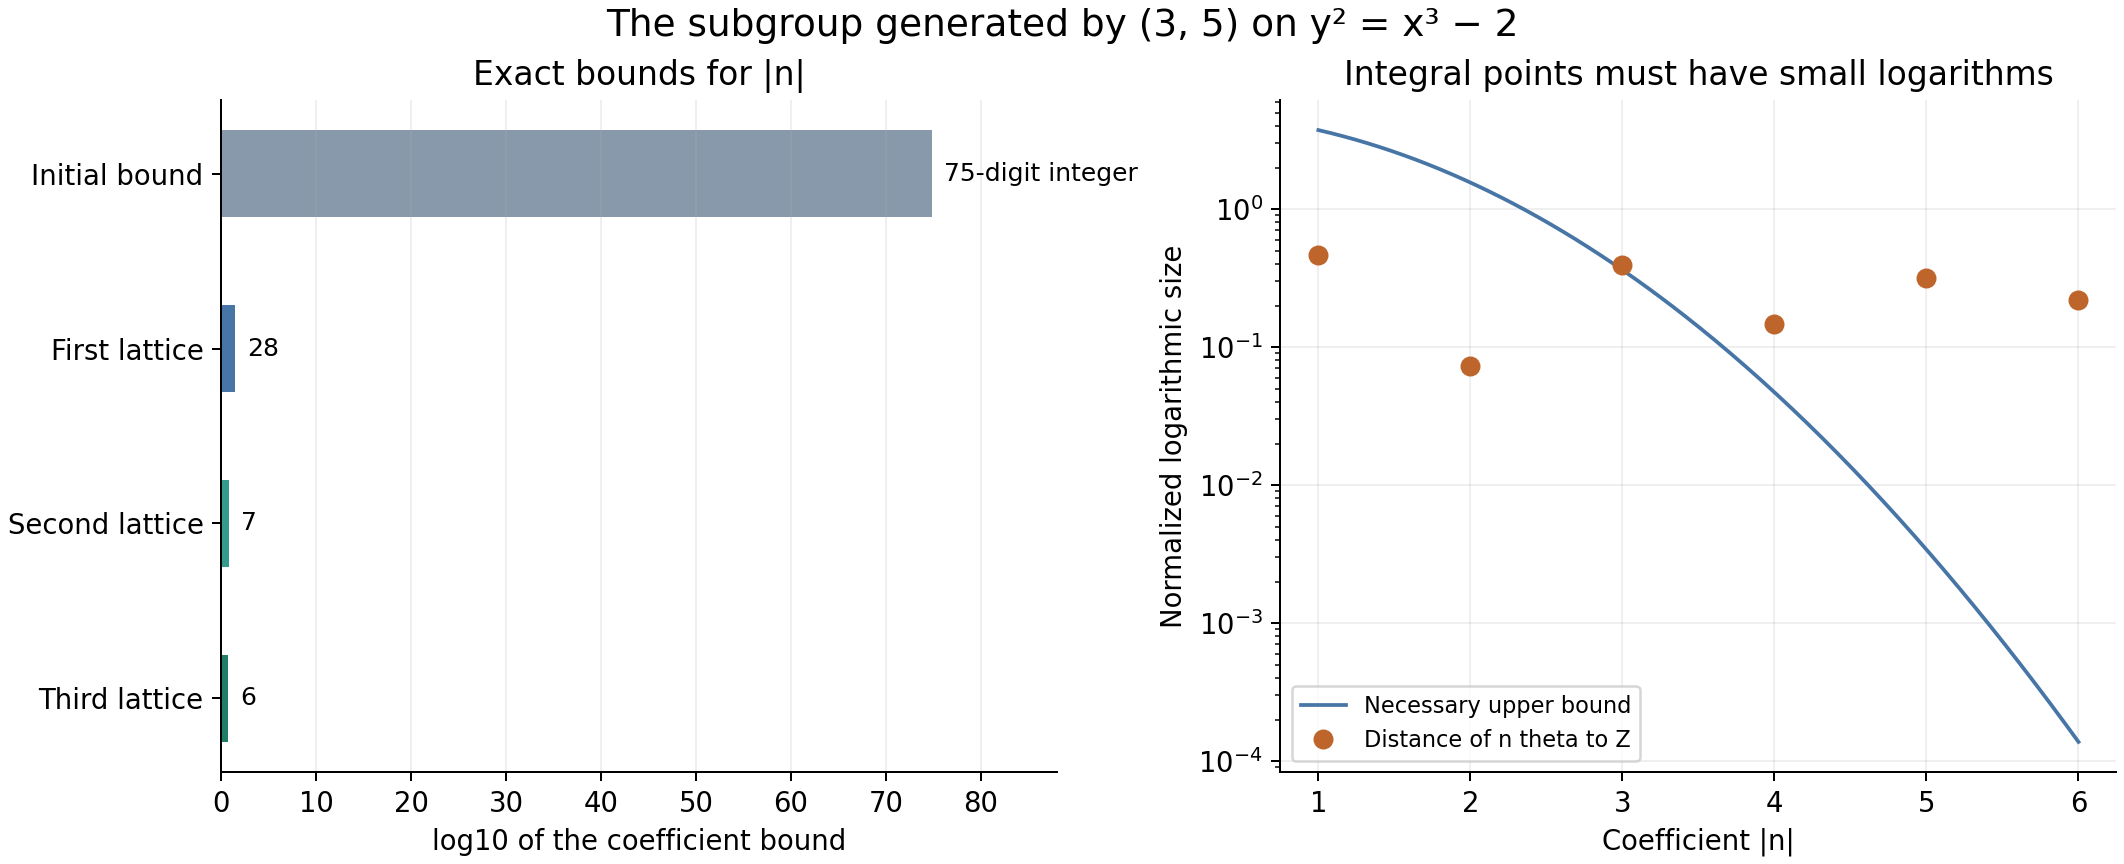
\includegraphics[keepaspectratio,alt={Coefficient bounds and the small-logarithm condition for a cyclic elliptic subgroup}]{../verification/lesson22/elliptic-integral-reduction.png}}
\par\smallskip
\begin{flushleft}\small
\emph{Figure 22.20. Left: the initial coefficient bound and the three
certified reductions in (22.703), on a logarithmic scale. Right: the
distance of \(n\theta\) to the nearest integer and the upper bound
\(5e^{-7n^2/24}\) necessary for an integral multiple with \(x\ge3\).
These plotted values are numerical displays of the objects in the proof.
The exact lattice and final rational-coordinate calculations establish
(22.704).}
\end{flushleft}
\end{minipage}\par\medskip


\subsubsection{Exercise 22.235. Independence does not prove
saturation}\label{exercise-22.235.-independence-does-not-prove-saturation}

On the curve in Example 22.234, show that \(2P\) is independent modulo
torsion but that searching only \(\mathbf Z(2P)\) misses an integral
point of \(\mathbf ZP\).

\textbf{Solution.} The positive value \(q(P)>7/8\) and (22.573) give
\(q(2P)=4q(P)>0\), so \(2P\) is nontorsion. If \(P=n(2P)\), then
\(q(P)=4n^2q(P)\), hence \(1=4n^2\), impossible for an integer \(n\).
Thus the integral point \(P\) is absent from \(\mathbf Z(2P)\), despite
the independence of that subgroup's generator. The index of this
subgroup in \(\mathbf ZP\) is two. \(\square\)

\subsection{Uniform bounds, effective enumeration and algebraic
independence}\label{uniform-bounds-effective-enumeration-and-algebraic-independence}

The height in this section is the absolute logarithmic Weil height, and
\(h^*(\alpha)=\max\{1,h(\alpha)\}\). At a place above a rational prime
\(p\), the valuation is normalized by \(v_p(p)=1\). All logarithms of
positive real numbers are real logarithms.

\subsubsection{Problem 22.236. The dependence on the
prime}\label{problem-22.236.-the-dependence-on-the-prime}

Fix positive integers \(n,D\). For each prime \(p\), define \[
 G_{n,D}(p)=\sup
 \frac{\max\{0,v_p(\alpha_1^{b_1}\cdots\alpha_n^{b_n}-1)\}\log p}
 {h^*(\alpha_1)\cdots h^*(\alpha_n)\log B},
 \qquad B=\max\{3,|b_1|,\ldots,|b_n|\}.
 \tag{22.705}
\] The supremum ranges over number fields \(K\) of degree at most \(D\),
places of \(K\) above \(p\), units at that place
\(\alpha_i\in K^\times\), and integers \(b_i\) for which the product is
different from one. A zero coefficient is allowed. Here a unit at the
place means \(v_p(\alpha_i)=0\), without requiring an algebraic integer
unit at every place.

One precise form of the prime-dependence problem is to obtain sharp,
effectively computable upper estimates for (22.705), uniformly in all
the data being varied. A specific question is whether, for every \(n,D\)
and every positive rational \(\varepsilon\), one can compute
\(A(n,D,\varepsilon)>0\) such that \[
 G_{n,D}(p)\le A(n,D,\varepsilon)p^\varepsilon
 \quad\hbox{for every prime }p.
 \tag{22.706}
\] This is a question, not an estimate assumed in any preceding proof.
The supremum and (22.706) specify a normalization of the general
problem; they are not a quotation of a named conjecture. For the prime
factors in existing local estimates, see Theorem 1.3 of
\href{https://arxiv.org/pdf/2209.00275}{Bugeaud, \emph{B'}}, pages 4--5.
Fixing \(p\) before choosing a constant would change the question.

A more specific conjecture is given by
\href{https://arxiv.org/pdf/math/0607072v3}{Yamada, Conjecture 1.3,
equation (8)}: except for finitely many pairs consisting of an integer
\(x>1\) and a prime \(p\), \[
 v_p(x^{p-1}-1)
 \le 2+\frac{\log x+2\log\log x+\log\log p}{\log p}.
 \tag{22.707}
\] The finite exceptional set here is over pairs, not a separately
unspecified infinite family for each prime. No effective bound for that
set is part of this formulation. Formula (22.707) concerns one special
family of coefficients; it does not by itself assert (22.706) for
general products.

\subsubsection{Proposition 22.237. Two benchmarks for prime
dependence}\label{proposition-22.237.-two-benchmarks-for-prime-dependence}

For every \(n,D\ge1\) and every prime \(p\), \[
 G_{n,D}(p)\ge
 \frac{\log p}{\log(p+1)\log3}.
 \tag{22.708}
\] For a fixed integer \(x>1\) and an odd prime \(p\nmid x\), the
unconditional estimate proved in Theorem 10.167 gives \[
 v_p(x^{p-1}-1)
 <283\frac{p}{(\log p)^2}\log(5x)\log5.
 \tag{22.709}
\] On the other hand, (22.707) would imply that, for each fixed \(x>1\),
\(v_p(x^{p-1}-1)\le2\) for all sufficiently large primes \(p\).

\textbf{Proof.} In (22.705) take \(K=\mathbb Q\), \(\alpha_1=p+1\),
\(b_1=1\), and pad with \(\alpha_i=1,b_i=0\). The product minus one is
\(p\), of valuation one, and \(h^*(p+1)=\log(p+1)\). This proves
(22.708). Its right side tends to \(1/\log3\); in particular a bound
tending to zero cannot hold with this normalization.

Apply
\href{TR-BAKER-10.html\#56-the-constant-283-for-fermat-differences-and-arbitrary-powers}{Theorem
10.167, equation (10.581)} with the coprime positive integers
\(a=x,b=1\) to obtain (22.709). The theorem includes \(b=1\). Finally,
for fixed \(x\), the fraction in (22.707) tends to zero as \(p\) tends
to infinity. For example \(\log t\le\sqrt t\) for \(t\ge4\), as follows
by differentiation, so \(\log t/t\longrightarrow0\). Outside the
finitely many exceptional pairs, the upper bound in (22.707) is
therefore less than three for large \(p\). The valuation is an integer,
giving the assertion. \(\square\)

\subsubsection{Problem 22.238. A specified constant for three real
logarithms}\label{problem-22.238.-a-specified-constant-for-three-real-logarithms}

For an integer \(D\ge1\), let \(C_3(D)\) be the supremum of \[
 \frac{\max\{0,-\log|\Lambda|\}}
 {h^*(\alpha_1)h^*(\alpha_2)h^*(\alpha_3)\log B},
 \quad
 \Lambda=\sum_{i=1}^3 b_i\log\alpha_i\ne0,
 \quad B=\max\{3,|b_1|,|b_2|,|b_3|\},
 \tag{22.710}
\] over positive real algebraic \(\alpha_i\) whose generated field has
degree at most \(D\), and integer coefficients \(b_i\). Determine
\(C_3(D)\), or give substantially closer explicit upper and lower bounds
with this same normalization. The exact constant and its growth with
\(D\) are distinct quantitative questions.

The positivity restriction fixes the logarithmic branches. A question
about arbitrary complex logarithms must also specify their sizes; one
cannot silently transfer (22.710) to arbitrary branches. For the source
context of improving three-logarithm estimates, see
\href{https://arxiv.org/pdf/2205.08899v3}{Mignotte and Voutier, with an
appendix by Laurent, \emph{A kit for linear forms in three logarithms}},
§§1.2--1.5. The optimization problem (22.710) fixes a common scale on
which constants can be compared. It does not presume that no sharper
specialized estimates exist, or that a bound established under
additional hypotheses applies to this entire supremum.

\subsubsection{Proposition 22.239. The three-logarithm constant is
finite and
positive}\label{proposition-22.239.-the-three-logarithm-constant-is-finite-and-positive}

For every \(D\ge1\), \[
 0<C_3(D)\le 2^{39}D^5\log(eD).
 \tag{22.711}
\]

\textbf{Proof.} Write \(d\le D\) for the degree of the generated field.
For a positive algebraic number, the selected archimedean place and the
identity \(h(\alpha^{-1})=h(\alpha)\) give
\(|\log\alpha|\le d h(\alpha)\). Both height facts are proved in
\href{../TR-TRANS/TR-TRANS-02.html\#4-height-arithmetic-and-finite-sets}{height
arithmetic}. Omit zero logarithms and zero coefficients, leaving
\(1\le r\le3\) terms. In
\href{TR-BAKER-08.html\#4-matveev-s-homogeneous-estimate}{Theorem
8.6} choose \(H_i=d h^*(\alpha_i)\), which satisfies every height and
logarithm cutoff. The field is real at the chosen embedding. The
unweighted coefficient version of that theorem and
\(C_1(r,1)\le2^{6r+20}\le2^{38}\) give \[
 \log|\Lambda|>
 -2^{38}d^{r+2}\log(ed)\log(eB)
       \prod_{i\text{ retained}}h^*(\alpha_i).
 \tag{22.712}
\] Since \(B\ge3>e\), \(\log(eB)\le2\log B\). The omitted height factors
are at least one, and \(d^{r+2}\le D^5\). Division by the denominator in
(22.710), followed by a supremum, proves the upper bound. Taking a
supremum changes the strict pointwise bound into a weak inequality, as
written in (22.711).

For positivity take \((\alpha_1,\alpha_2,\alpha_3)=(2,3,5)\) and
\((b_1,b_2,b_3)=(1,1,-1)\). Then \(0<\Lambda=\log(6/5)<1\), so its
quotient in (22.710) is positive. These rational bases are allowed for
every \(D\ge1\). \(\square\)

\subsubsection{Problem 22.240. Effective
Mordell}\label{problem-22.240.-effective-mordell}

Give a terminating algorithm with the following input and output. The
input is a number field \(K\), represented by exact algebraic data, and
homogeneous equations for a smooth, projective, geometrically integral
curve \(C\subset\mathbb P^N_K\) of genus at least two. The output is an
integer \(H\ge1\) such that \[
 H_{\mathbb P^N}(P)\le H\quad\hbox{for every }P\in C(K),
 \tag{22.713}
\] where \(H_{\mathbb P^N}=\exp h_{\mathbb P^N}\) is the absolute
multiplicative projective height for the given embedding. The algorithm
must work for every such input, without a conjectural termination
assumption or an additional restriction on the rank of the Jacobian.

This is the general effective Mordell problem in height form. A free
primary account of its scope and approaches is
\href{https://arxiv.org/pdf/2503.10443v2}{Garcia-Fritz and Pasten,
\emph{Effective Mordell for curves with enough automorphisms}}, §§1.1
and 1.3. Its additional automorphism and rank hypotheses matter: that
setting is a restricted class within the problem above. Likewise,
Proposition 22.232 addresses integral points on an elliptic curve with
supplied generators. It does not produce (22.713) for all rational
points on arbitrary higher-genus curves.

\subsubsection{Proposition 22.241. A height cutoff is a stopping
certificate over the
rationals}\label{proposition-22.241.-a-height-cutoff-is-a-stopping-certificate-over-the-rationals}

For curves over \(\mathbb Q\), an algorithm producing (22.713) gives a
terminating algorithm listing all rational points. Conversely, a
terminating algorithm producing the complete finite list gives an
algorithm producing (22.713).

\textbf{Proof.} Every point of \(\mathbb P^N(\mathbb Q)\) has a unique
integer coordinate vector \((a_0,\ldots,a_N)\) whose coordinates have
greatest common divisor one and whose first nonzero coordinate is
positive. To obtain it, clear denominators, divide by the common divisor
and fix the sign. Two primitive integer vectors representing the same
projective point differ by a rational scalar. Writing the scalar as a
reduced fraction shows, from primitivity of both vectors, that it is
\(1\) or \(-1\); the sign convention removes the latter possibility. In
these coordinates, \[
 H_{\mathbb P^N}([a_0:\cdots:a_N])=\max_i|a_i|.
 \tag{22.714}
\] Indeed at every finite prime at least one coordinate is a unit, so
its local maximum is one; the remaining archimedean factor is the
displayed maximum. This also agrees with the projective height
normalization in Proposition 22.49.

Enumerate the finite box \([-H,H]^{N+1}\cap\mathbb Z^{N+1}\), remove the
zero vector and the vectors violating primitivity or the sign
convention, and test the homogeneous equations by exact rational
arithmetic. Formula (22.714) proves coverage and uniqueness. In the
reverse direction, compute the maximum of the coordinate heights on the
returned finite list; use one if the list is empty. \(\square\)

A bound for the number of points alone does not give this coordinate
cutoff. Even a singleton set of projective rational points can have
arbitrarily large height: \(\{[1:M]\}\) has one point and height \(M\)
for every integer \(M\ge1\). Nor does an unbounded search announce that
it has found its last point.

\subsubsection{Conjecture 22.242.
Schanuel}\label{conjecture-22.242.-schanuel}

If \(z_1,\ldots,z_m\in\mathbb C\) are linearly independent over
\(\mathbb Q\), then \[
 \operatorname{trdeg}_{\mathbb Q}
 \mathbb Q(z_1,\ldots,z_m,e^{z_1},\ldots,e^{z_m})\ge m.
 \tag{22.715}
\] The quantifier includes arbitrary complex numbers, not only
logarithms of algebraic numbers. See
\href{https://webusers.imj-prg.fr/~michel.waldschmidt/articles/pdf/odp.pdf}{Waldschmidt,
\emph{Open Diophantine Problems}, Conjecture 3.1, printed page 267}. No
conclusion below that assumes (22.715) is an unconditional use of the
analytic subgroup theorem.

\subsubsection{Proposition 22.243. Conditional algebraic
independence}\label{proposition-22.243.-conditional-algebraic-independence}

Assume (22.715). If \(\lambda_1,\ldots,\lambda_m\) are
\(\mathbb Q\)-linearly independent and every \(e^{\lambda_i}\) is
algebraic, then the \(\lambda_i\) are algebraically independent over
\(\overline{\mathbb Q}\). In particular \(\log2,\log3\) are
algebraically independent. Also \(e,\pi\) are algebraically independent.

\textbf{Proof.} We use the elementary fact that a field algebraic over a
rational function field in \(r\) independent variables has no \(r+1\)
algebraically independent elements. Here is a finite dimensional proof
of the needed direction. Any proposed finite tuple is contained in a
finite extension of that function field. In a basis of this finite
extension, multiplication by each tuple element is a matrix of rational
functions. Choose a common polynomial denominator for their entries.
Products with every exponent at most \(M\), applied to the coordinate
vector of one, have, after multiplication by one common denominator
power, polynomial coordinates of degree at most \(cM+c\), for a constant
\(c\) independent of \(M\). Their rational span has dimension at most
the basis size times \(\binom{cM+c+r}{r}\). For \(r+1\) elements there
are \((M+1)^{r+1}\) such products. This eventually exceeds that
dimension, which grows with degree \(r\), and gives a nonzero polynomial
relation with rational coefficients.

Choose a maximal algebraically independent subtuple of the
\(\lambda_i\), of size \(r\). Every other \(\lambda_i\) is algebraic
over its rational function field: a polynomial relation with the maximal
subtuple becomes a nonzero polynomial in that one extra element, since
the subtuple is independent. Adjoining the algebraic \(e^{\lambda_i}\)
does not change this property. The preceding dimension argument,
together with (22.715), gives \(r\ge m\). Thus \(r=m\), proving
independence over \(\mathbb Q\).

It also implies independence over \(\overline{\mathbb Q}\). Otherwise
let a nonzero vanishing polynomial have its coefficients in a finite
Galois extension \(L/\mathbb Q\). The product of its coefficient
conjugates over \(\operatorname{Gal}(L/\mathbb Q)\) is a nonzero
polynomial with rational coefficients. It still vanishes at the tuple,
because one factor does. This contradicts independence over
\(\mathbb Q\).

If \(a\log2+b\log3=0\) for integers \(a,b\), exponentiation and unique
prime factorization give \(a=b=0\). Clearing denominators proves their
rational linear independence, so the first assertion applies. For
\(e,\pi\), apply (22.715) to \(1,i\pi\), which are rationally
independent by their real and imaginary parts. Their exponentials are
\(e,-1\). Consequently \(\mathbb Q(i\pi,e)\) has transcendence degree at
least two. Adjoining the algebraic number \(i\) identifies its algebraic
extension with an algebraic extension of \(\mathbb Q(\pi,e)\). If
\(\pi,e\) were dependent, a maximal independent subtuple would have size
at most one, contradicting the same dimension argument. \(\square\)

The logarithm assertion is Conjecture 3.3 in Waldschmidt's account; the
proof above establishes it conditional on Schanuel. Algebraic
independence forbids every nonzero polynomial relation. Linear
independence over algebraic coefficients, as supplied earlier by the
analytic subgroup theorem, forbids only relations of degree one. No
polynomial version follows just by replacing the word ``linear''.

\subsubsection{Exercise 22.244. The coefficient size cannot
disappear}\label{exercise-22.244.-the-coefficient-size-cannot-disappear}

Let \(p\) be an odd prime, \(a\ge1\), \(k\ge0\), and let \(m\) be a
positive integer prime to \(p\). Prove \[
 v_p((1+p^a)^{p^k m}-1)=a+k.
 \tag{22.716}
\] Explain why a bound independent of the coefficients is impossible
even for fixed \(p\) and a fixed rational base. Determine the limiting
quotient in (22.705) for this example with \(m=1\) as
\(k\longrightarrow\infty\).

\textbf{Solution (medium).} If \(u=1+c p^s\), \(s\ge1\), and
\(p\nmid c\), then the first term of \(u^p-1\) is \(c p^{s+1}\). For
\(2\le j<p\), the binomial coefficient \(\binom pj\) is divisible by
\(p\), so the corresponding term has valuation at least \(1+2s\ge s+2\).
The last term has valuation \(ps\ge s+2\). Thus \(v_p(u^p-1)=s+1\).
Induction gives \(a+k\) after the \(p^k\)-th power. Raising to the
prime-to-\(p\) power \(m\) preserves that valuation: its first binomial
term has valuation \(a+k\), and all later terms have strictly larger
valuation. This proves (22.716).

With \(p,a\) fixed, the valuation grows without bound with \(k\). For
\(m=1\) and \(k\ge1\), \(B=p^k\) and \(h^*(1+p^a)=\log(1+p^a)\). The
quotient is therefore \((a+k)/(k\log(1+p^a))\), tending to
\(1/\log(1+p^a)\). The factor \(\log B\) has a concrete role even before
one asks about the dependence on the prime.

\subsubsection{Exercise 22.245. A finite projective
search}\label{exercise-22.245.-a-finite-projective-search}

Apply the enumeration in Proposition 22.241 to \(X^2+Y^2=Z^2\) with
supplied height bound five. List every projective rational point in that
box. This exercise concerns a given cutoff on a conic, and makes no
higher-genus height claim.

\textbf{Solution (easy).} A primitive vector with a zero coordinate is
one of \[
 [1:0:1],\ [1:0:-1],\ [0:1:1],\ [0:1:-1].
 \tag{22.717}
\] If both \(X,Y\) are nonzero, use absolute values. Among the squares
\(1,4,9,16,25\), the only sum of two positive squares that is a square
at most 25 is \(9+16=25\). Thus the remaining points, with the sign
convention of Proposition 22.241, are \[
 [3:\pm4:\pm5],\qquad [4:\pm3:\pm5],
 \tag{22.718}
\] with the two signs chosen independently. These eight points and the
four in (22.717) are all twelve points of height at most five. The
finite comparison of squares, the gcd condition and the sign
normalization prove completeness within the stated box.

\end{document}
